\documentclass[twoside]{book}

% Packages required by doxygen
\usepackage{fixltx2e}
\usepackage{calc}
\usepackage{doxygen}
\usepackage[export]{adjustbox} % also loads graphicx
\usepackage{graphicx}
\usepackage[utf8]{inputenc}
\usepackage{makeidx}
\usepackage{multicol}
\usepackage{multirow}
\PassOptionsToPackage{warn}{textcomp}
\usepackage{textcomp}
\usepackage[nointegrals]{wasysym}
\usepackage[table]{xcolor}

% Font selection
\usepackage[T1]{fontenc}
\usepackage[scaled=.90]{helvet}
\usepackage{courier}
\usepackage{amssymb}
\usepackage{sectsty}
\renewcommand{\familydefault}{\sfdefault}
\allsectionsfont{%
  \fontseries{bc}\selectfont%
  \color{darkgray}%
}
\renewcommand{\DoxyLabelFont}{%
  \fontseries{bc}\selectfont%
  \color{darkgray}%
}
\newcommand{\+}{\discretionary{\mbox{\scriptsize$\hookleftarrow$}}{}{}}

% Page & text layout
\usepackage{geometry}
\geometry{%
  a4paper,%
  top=2.5cm,%
  bottom=2.5cm,%
  left=2.5cm,%
  right=2.5cm%
}
\tolerance=750
\hfuzz=15pt
\hbadness=750
\setlength{\emergencystretch}{15pt}
\setlength{\parindent}{0cm}
\setlength{\parskip}{3ex plus 2ex minus 2ex}
\makeatletter
\renewcommand{\paragraph}{%
  \@startsection{paragraph}{4}{0ex}{-1.0ex}{1.0ex}{%
    \normalfont\normalsize\bfseries\SS@parafont%
  }%
}
\renewcommand{\subparagraph}{%
  \@startsection{subparagraph}{5}{0ex}{-1.0ex}{1.0ex}{%
    \normalfont\normalsize\bfseries\SS@subparafont%
  }%
}
\makeatother

% Headers & footers
\usepackage{fancyhdr}
\pagestyle{fancyplain}
\fancyhead[LE]{\fancyplain{}{\bfseries\thepage}}
\fancyhead[CE]{\fancyplain{}{}}
\fancyhead[RE]{\fancyplain{}{\bfseries\leftmark}}
\fancyhead[LO]{\fancyplain{}{\bfseries\rightmark}}
\fancyhead[CO]{\fancyplain{}{}}
\fancyhead[RO]{\fancyplain{}{\bfseries\thepage}}
\fancyfoot[LE]{\fancyplain{}{}}
\fancyfoot[CE]{\fancyplain{}{}}
\fancyfoot[RE]{\fancyplain{}{\bfseries\scriptsize Generated by Doxygen }}
\fancyfoot[LO]{\fancyplain{}{\bfseries\scriptsize Generated by Doxygen }}
\fancyfoot[CO]{\fancyplain{}{}}
\fancyfoot[RO]{\fancyplain{}{}}
\renewcommand{\footrulewidth}{0.4pt}
\renewcommand{\chaptermark}[1]{%
  \markboth{#1}{}%
}
\renewcommand{\sectionmark}[1]{%
  \markright{\thesection\ #1}%
}

% Indices & bibliography
\usepackage{natbib}
\usepackage[titles]{tocloft}
\setcounter{tocdepth}{3}
\setcounter{secnumdepth}{5}
\makeindex

% Hyperlinks (required, but should be loaded last)
\usepackage{ifpdf}
\ifpdf
  \usepackage[pdftex,pagebackref=true]{hyperref}
\else
  \usepackage[ps2pdf,pagebackref=true]{hyperref}
\fi
\hypersetup{%
  colorlinks=true,%
  linkcolor=blue,%
  citecolor=blue,%
  unicode%
}

% Custom commands
\newcommand{\clearemptydoublepage}{%
  \newpage{\pagestyle{empty}\cleardoublepage}%
}

\usepackage{caption}
\captionsetup{labelsep=space,justification=centering,font={bf},singlelinecheck=off,skip=4pt,position=top}

%===== C O N T E N T S =====

\begin{document}

% Titlepage & ToC
\hypersetup{pageanchor=false,
             bookmarksnumbered=true,
             pdfencoding=unicode
            }
\pagenumbering{roman}
\begin{titlepage}
\vspace*{7cm}
\begin{center}%
{\Large Merlin \\[1ex]\large 1.\+0 }\\
\vspace*{1cm}
{\large Generated by Doxygen 1.8.11}\\
\end{center}
\end{titlepage}
\clearemptydoublepage
\tableofcontents
\clearemptydoublepage
\pagenumbering{arabic}
\hypersetup{pageanchor=true}

%--- Begin generated contents ---
\chapter{Description}
\label{md_README}
\hypertarget{md_README}{}
\hyperlink{classMerlin}{Merlin} is a standalong solver written in {\ttfamily C++} that implements state-\/of-\/the-\/art exact and approximate algorithms for probabilistic inference over graphical models including both directed and undirected models (e.\+g., Bayesian networks, Markov Random Fields). It can be used for many applications and research in bioinformatics, computer vision, or speech and language processing to name a few. \hyperlink{classMerlin}{Merlin} supports the most common probabilistic inference tasks such as computing the partition function or probability of evidence (PR), posterior marginals (M\+AP), as well as M\+AP (also known as maximum aposteriori or most probable explanation) and marginal M\+AP configurations.

\hyperlink{classMerlin}{Merlin} implements the classic Loopy Belief Propagation (L\+BP) algorithm as well as more advanced generalized belief propagation algorithms such as Iterative Join-\/\+Graph Propagation (I\+J\+GP) and Weighted Mini-\/\+Bucket Elimination (W\+MB). The default algorithm for computing all four probabilistic inference tasks (PR, M\+AR, M\+AP, M\+M\+AP) is W\+M\+B(i). The algorithm is parameterized by an i-\/bound that allows for a controllable tradeoff between accuracy of the results and the computational cost. Larger values of the i-\/bound typically yield more accurate results but it takes more time and memory to compute them. Selecting a large enough i-\/bound allows for exact inference (i.\+e., i-\/bound equal to the treewidth of the model). For relatively small i-\/bounds \hyperlink{classMerlin}{Merlin} performs approximate inference.

\section*{A\+PI}

\subsection*{\hyperlink{classMerlin}{Merlin} A\+PI}

Class {\ttfamily \hyperlink{classMerlin}{Merlin}} defined in {\ttfamily \hyperlink{merlin_8h}{merlin.\+h}} header exposes most of the functionality of the solver. A graphical model is a collection of factors (or positive real-\/valued functions) defined over subsets of variables. Variables are assumed to be indexed from {\ttfamily 0}.

\subsubsection*{Methods}

\begin{DoxyVerb}    bool read_model(const char* f)
\end{DoxyVerb}
 This method loads the graphical model from a file which is specified using the U\+AI format (see also the File Formats section). Returns {\ttfamily true} if successful and {\ttfamily false} otherwise. \begin{DoxyVerb}    bool read_evidence(const char* f)
\end{DoxyVerb}
 This method loads the evidence variables and their corresponding observed values from a file which is also specified using the U\+AI format. Returns {\ttfamily true} if successful, and {\ttfamily false} otherwise. \begin{DoxyVerb}    bool read_query(const char* f)
\end{DoxyVerb}
 This method loads the query variables from a file specified using the U\+AI format. The query variables (also known as M\+AX of M\+AP variables) are only specific to Marginal M\+AP (M\+M\+AP) inference tasks. Returns {\ttfamily true} if successful, and {\ttfamily false} otherwise. \begin{DoxyVerb}    bool set_task(size_t t)
\end{DoxyVerb}
 This method sets the probabilistic inference task to be solved. The possible values for the {\ttfamily t} parameter are\+:
\begin{DoxyItemize}
\item {\ttfamily M\+E\+R\+L\+I\+N\+\_\+\+T\+A\+S\+K\+\_\+\+PR} \+: Partition function (probability of evidence)
\item {\ttfamily M\+E\+R\+L\+I\+N\+\_\+\+T\+A\+S\+K\+\_\+\+M\+AR} \+: Posterior marginals (given evidence)
\item {\ttfamily M\+E\+R\+L\+I\+N\+\_\+\+T\+A\+S\+K\+\_\+\+M\+AP} \+: Maximum aposteriori (given evidence)
\item {\ttfamily M\+E\+R\+L\+I\+N\+\_\+\+T\+A\+S\+K\+\_\+\+M\+M\+AP} \+: Marginal M\+AP (given evidence) \begin{DoxyVerb}  bool set_algorithm(size_t a)
\end{DoxyVerb}
 This method sets the the algorithm to be used when solving the selected probabilistic inference task. The possible values for the {\ttfamily a} parameter are\+:
\item {\ttfamily M\+E\+R\+L\+I\+N\+\_\+\+A\+L\+G\+O\+\_\+\+G\+I\+B\+BS} \+: Gibbs sampling
\item {\ttfamily M\+E\+R\+L\+I\+N\+\_\+\+A\+L\+G\+O\+\_\+\+L\+BP} \+: Loopy belief propagation
\item {\ttfamily M\+E\+R\+L\+I\+N\+\_\+\+A\+L\+G\+O\+\_\+\+I\+J\+GP} \+: Iterative join graph propagation
\item {\ttfamily M\+E\+R\+L\+I\+N\+\_\+\+A\+L\+G\+O\+\_\+\+J\+G\+LP} \+: Join graph linear programming
\item {\ttfamily M\+E\+R\+L\+I\+N\+\_\+\+A\+L\+G\+O\+\_\+\+W\+MB} \+: Weighted mini-\/bucket elimination
\item {\ttfamily M\+E\+R\+L\+I\+N\+\_\+\+A\+L\+G\+O\+\_\+\+A\+O\+BB} \+: A\+N\+D/\+OR branch and bound search (not implemented yet)
\item {\ttfamily M\+E\+R\+L\+I\+N\+\_\+\+A\+L\+G\+O\+\_\+\+A\+O\+BF} \+: Best-\/first A\+N\+D/\+OR search (not implemented yet)
\item {\ttfamily M\+E\+R\+L\+I\+N\+\_\+\+A\+L\+G\+O\+\_\+\+R\+B\+F\+A\+OO} \+: Recursive best-\/first A\+N\+D/\+OR search (not implemented yet) \begin{DoxyVerb}  void set_param_ibound(size_t ibound)
\end{DoxyVerb}
 This method sets the i-\/bound parameter which is used by the following algorithms\+: {\ttfamily W\+MB}, {\ttfamily I\+J\+GP}, {\ttfamily J\+G\+LP} (as well as search based ones {\ttfamily A\+O\+BB}, {\ttfamily A\+O\+BF}, and {\ttfamily R\+B\+F\+A\+OO}). The default value is {\ttfamily 4}. \begin{DoxyVerb}    void set_param_iterations(size_t iter)
\end{DoxyVerb}
 This method sets the number of iterations to be executed by the inference algorithm. The parameter is specific to the following algorithms\+: {\ttfamily W\+MB}, {\ttfamily I\+J\+GP}, {\ttfamily J\+G\+LP}, and {\ttfamily L\+BP}. The default value is {\ttfamily 100}. For Gibbs sampling consider runnig several thousands of iterations. \begin{DoxyVerb}    void set_param_samples(size_t s)
\end{DoxyVerb}
 This method sets the number of samples to be generated in each iteration of the {\ttfamily G\+I\+B\+BS} sampling algorithm. The default value is {\ttfamily 100}. \begin{DoxyVerb}    void run()
\end{DoxyVerb}
 This method runs the inference algorithm for the selected task on the input graphical model and evidence (if any). The output is generated into a file specified using the U\+AI format. The name of the output file is obtained from the input file augmented with the {\ttfamily task.\+out} suffix, where {\ttfamily task} corresponds to one of the follwing\+: {\ttfamily PR}, {\ttfamily M\+AR}, {\ttfamily M\+AP}, or {\ttfamily M\+M\+AP}.
\end{DoxyItemize}

\section*{Source Code}

The source code is organized along the following directory structure and requires a standard G\+NU build using the G\+NU Autotools toolchain.


\begin{DoxyItemize}
\item {\ttfamily src/} -\/ contains the source (.cpp) files
\item {\ttfamily src/include/} -\/ contains the header (.h) files
\item {\ttfamily data/} -\/ contains several example graphical models
\item {\ttfamily doc/} -\/ contains the documentation
\end{DoxyItemize}

\section*{Build}

The simplest way to compile the solver is to import the Eclipse project into Eclipse C\+DT and compile it in Release or Debug mode.

\subsection*{Building the Documentation}

\hyperlink{classMerlin}{Merlin} uses Doxygen to build automatically the reference manual of the library, and supports both {\ttfamily html} and {\ttfamily latex} (see the corresponding {\ttfamily doc/html} and {\ttfamily doc/latex} subfolders).

To build the entire documentation, simply run {\ttfamily doxygen merlin.\+doxygen} in the main folder {\ttfamily merlin/}. To generate the pdf run {\ttfamily make all} in the {\ttfamily doc/latex} subfolder).

\section*{File Formats}

\subsection*{Input File Format}

\hyperlink{classMerlin}{Merlin} uses a simple text file format which is specified below to describe a problem instances (i.\+e., graphical model). The format is identical to the one used during the U\+AI Inference competitions.

\subsubsection*{Structure}

The input file format consists of the following two parts, in that order\+: \begin{DoxyVerb}    <Preamble>
    <Factors>
\end{DoxyVerb}


The contents of each section (denoted $<$ …$>$=\char`\"{}\char`\"{}$>$ above) are described in the following\+:

\paragraph*{Preamble}

The description of the format will follow a simple Markov network with three variables and two functions. A sample preamble for such a network is\+: \begin{DoxyVerb}    MARKOV
    3
    2 2 3
    2
    2 0 1
    2 1 2
\end{DoxyVerb}


The preamble starts with one line denoting the type of network. Generally, this can be either B\+A\+Y\+ES (if the network is a Bayesian network) or M\+A\+R\+K\+OV (in case of a Markov network).

The second line contains the number of variables.

The third line specifies the cardinalities of each variable, one at a time, separated by a whitespace (note that this implies an order on the variables which will be used throughout the file).

The fourth line contains only one integer, denoting the number of cliques in the problem. Then, one clique per line, the scope of each clique is given as follows\+: The first integer in each line specifies the number of variables in the clique, followed by the actual indexes of the variables. The order of this list is not restricted (for Bayesian networks we assume that the child variable of the clique is the last one). Note that the ordering of variables within a factor will follow the order provided here.

Referring to the example above, the first line denotes the Markov network, the second line tells us the problem consists of three variables, let\textquotesingle{}s refer to them as {\ttfamily X}, {\ttfamily Y}, and {\ttfamily Z}. Their cardinalities are {\ttfamily 2}, {\ttfamily 2}, and {\ttfamily 3} respectively (from the third line). Line four specifies that there are 2 cliques. The first clique is {\ttfamily X,Y}, while the second clique is {\ttfamily Y,Z}. Note that variables are indexed starting with {\ttfamily 0}.

\paragraph*{Factors}

Each factor is specified by giving its full table (i.\+e, specifying a non-\/negative real value for each assignment). The order of the factors is identical to the one in which they were introduced in the preamble, the first variable has the role of the \textquotesingle{}most significant\textquotesingle{} digit. For each factor table, first the number of entries is given (this should be equal to the product of the domain sizes of the variables in the scope). Then, one by one, separated by whitespace, the values for each assignment to the variables in the factor\textquotesingle{}s scope are enumerated. Tuples are implicitly assumed in ascending order, with the last variable in the scope as the {\ttfamily least significant}. To illustrate, we continue with our Markov network example from above, let\textquotesingle{}s assume the following conditional probability tables\+: \begin{DoxyVerb}    X | P(X)  
    0 | 0.436 
    1 | 0.564 

    X   Y |  P(Y,X)
    0   0 |  0.128
    0   1 |  0.872
    1   0 |  0.920
    1   1 |  0.080

    Y   Z |  P(Z,Y)
    0   0 |  0.210
    0   1 |  0.333
    0   2 |  0.457
    1   0 |  0.811
    1   1 |  0.000
    1   2 |  0.189
\end{DoxyVerb}


Then we have the corresponding file content\+: \begin{DoxyVerb}    2
     0.436 0.564

    4
     0.128 0.872
     0.920 0.080

    6
     0.210 0.333 0.457
     0.811 0.000 0.189
\end{DoxyVerb}


Note that line breaks and empty lines are effectively just a whitespace, exactly like plain spaces “ ”. They are used here to improve readability.

\subsection*{Evidence File Format}

Evidence is specified in a separate file. The evidence file consists of a single line. The line will begin with the number of observed variables in the sample, followed by pairs of variable and its observed value. The indexes correspond to the ones implied by the original problem file.

If, for our example Markov network, {\ttfamily Y} has been observed as having its first value and {\ttfamily Z} with its second value, the evidence file would contain the following line\+: \begin{DoxyVerb}    2 1 0 2 1
\end{DoxyVerb}


\subsection*{Query File Format}

Query variables for Marginal M\+AP inference are specified in a separate file. The query file consists of a single line. The line will begin with the number of query variables, followed by the indexes of the query variables. The indexes correspond to the ones implied by the original problem file.

If, for our example Markov network, we want to use {\ttfamily Y} as the query variable the query file would contain the following line\+: \begin{DoxyVerb}    1 1
\end{DoxyVerb}


\subsection*{Output File Format}

The first line must contain only the task solved\+: {\ttfamily P\+R$\vert$\+M\+A\+P$\vert$\+M\+A\+R$\vert$\+M\+M\+AP}. The rest of the file will contain the solution for the task. Solvers can write more then one solution by writing {\ttfamily -\/\+B\+E\+G\+I\+N-\/} at the head of the new solution. In the example below the task we choose is {\ttfamily PR}. We have two solutions. The format of the {\ttfamily $<$S\+O\+L\+U\+T\+I\+ON$>$} part will be described below. \begin{DoxyVerb}    PR
    <SOLUTION>
    -BEGIN-
    <SOLUTION>
\end{DoxyVerb}


The solution format are as follows depending on the task\+:

\subsubsection*{Partition function {\ttfamily PR}}

Line with the value of the log10 of the partition function. For example, an approximation {\ttfamily log10 Pr(e) = -\/0.\+2008}which is known to be an upper bound may have a solution line\+: \begin{DoxyVerb}    -0.2008
\end{DoxyVerb}
 \subsubsection*{Maximum aposteriori {\ttfamily M\+AP}}

A space separated line that includes\+:
\begin{DoxyItemize}
\item the number {\ttfamily n} of model variables, and
\item the M\+AP instantiation, a list of value indices for all {\ttfamily n} variables.
\end{DoxyItemize}

For example, an input model with 3 binary variables may have a solution line\+: \begin{DoxyVerb}    3 0 1 0
\end{DoxyVerb}


\subsubsection*{Marginals {\ttfamily M\+AR}}

A space separated line that includes\+:
\begin{DoxyItemize}
\item the number of variables {\ttfamily n} in the model, and
\item a list of marginal approximations of all the variables. For each variable its cardinality is first stated, then the probability of each state is stated. The order of the variables is the same as in the model, all data is space separated.
\end{DoxyItemize}

For example, a model with {\ttfamily 3} variables, with cardinalities of {\ttfamily 2}, {\ttfamily 2}, {\ttfamily 3} respectively. The solution might look like this\+: \begin{DoxyVerb}    3 2 0.1 0.9 2 0.3 0.7 3 0.2 0.2 0.6
\end{DoxyVerb}


\subsubsection*{Marginal M\+AP {\ttfamily M\+M\+AP}}

A space separated line that includes\+:
\begin{DoxyItemize}
\item the number {\ttfamily q} of query (or M\+AP) variables, and
\item their most probable instantiation, a list of variable value pairs for all {\ttfamily q} variables.
\end{DoxyItemize}

For example, if the solution is an assignment of {\ttfamily 0}, {\ttfamily 1} and {\ttfamily 0} to three query variables indexed by {\ttfamily 2} {\ttfamily 3} and {\ttfamily 4} respectively, the solution will look as follows\+: \begin{DoxyVerb}    3 2 0 3 1 4 0 \end{DoxyVerb}
 
\chapter{Namespace Index}
\section{Namespace List}
Here is a list of all documented namespaces with brief descriptions\+:\begin{DoxyCompactList}
\item\contentsline{section}{\hyperlink{namespacemerlin}{merlin} \\*The default namespace of the library }{\pageref{namespacemerlin}}{}
\end{DoxyCompactList}

\chapter{Hierarchical Index}
\section{Class Hierarchy}
This inheritance list is sorted roughly, but not completely, alphabetically\+:\begin{DoxyCompactList}
\item \contentsline{section}{merlin\+:\+:factor\+\_\+graph\+:\+:abstract\+\_\+queue$<$ T $>$}{\pageref{classmerlin_1_1factor__graph_1_1abstract__queue}}{}
\begin{DoxyCompactList}
\item \contentsline{section}{merlin\+:\+:factor\+\_\+graph\+:\+:abstract\+\_\+queue\+\_\+fifo$<$ T $>$}{\pageref{classmerlin_1_1factor__graph_1_1abstract__queue__fifo}}{}
\item \contentsline{section}{merlin\+:\+:factor\+\_\+graph\+:\+:abstract\+\_\+queue\+\_\+lifo$<$ T $>$}{\pageref{classmerlin_1_1factor__graph_1_1abstract__queue__lifo}}{}
\end{DoxyCompactList}
\item \contentsline{section}{merlin\+:\+:algorithm}{\pageref{classmerlin_1_1algorithm}}{}
\begin{DoxyCompactList}
\item \contentsline{section}{merlin\+:\+:bte}{\pageref{classmerlin_1_1bte}}{}
\item \contentsline{section}{merlin\+:\+:gibbs}{\pageref{classmerlin_1_1gibbs}}{}
\item \contentsline{section}{merlin\+:\+:ijgp}{\pageref{classmerlin_1_1ijgp}}{}
\item \contentsline{section}{merlin\+:\+:jglp}{\pageref{classmerlin_1_1jglp}}{}
\item \contentsline{section}{merlin\+:\+:lbp}{\pageref{classmerlin_1_1lbp}}{}
\item \contentsline{section}{merlin\+:\+:wmb}{\pageref{classmerlin_1_1wmb}}{}
\end{DoxyCompactList}
\item \contentsline{section}{merlin\+:\+:factor\+:\+:bin\+Op\+Divide}{\pageref{structmerlin_1_1factor_1_1binOpDivide}}{}
\item \contentsline{section}{merlin\+:\+:factor\+:\+:bin\+Op\+Minus}{\pageref{structmerlin_1_1factor_1_1binOpMinus}}{}
\item \contentsline{section}{merlin\+:\+:factor\+:\+:bin\+Op\+Plus}{\pageref{structmerlin_1_1factor_1_1binOpPlus}}{}
\item \contentsline{section}{merlin\+:\+:factor\+:\+:bin\+Op\+Power}{\pageref{structmerlin_1_1factor_1_1binOpPower}}{}
\item \contentsline{section}{merlin\+:\+:factor\+:\+:bin\+Op\+Times}{\pageref{structmerlin_1_1factor_1_1binOpTimes}}{}
\item \contentsline{section}{merlin\+:\+:variable\+\_\+set\+:\+:const\+\_\+iterator}{\pageref{classmerlin_1_1variable__set_1_1const__iterator}}{}
\item \contentsline{section}{merlin\+:\+:convert\+\_\+index}{\pageref{classmerlin_1_1convert__index}}{}
\item \contentsline{section}{merlin\+:\+:edge\+\_\+id}{\pageref{structmerlin_1_1edge__id}}{}
\item \contentsline{section}{merlin\+:\+:factor}{\pageref{classmerlin_1_1factor}}{}
\item \contentsline{section}{merlin\+:\+:graph}{\pageref{classmerlin_1_1graph}}{}
\begin{DoxyCompactList}
\item \contentsline{section}{merlin\+:\+:graphical\+\_\+model}{\pageref{classmerlin_1_1graphical__model}}{}
\begin{DoxyCompactList}
\item \contentsline{section}{merlin\+:\+:bte}{\pageref{classmerlin_1_1bte}}{}
\item \contentsline{section}{merlin\+:\+:factor\+\_\+graph}{\pageref{classmerlin_1_1factor__graph}}{}
\begin{DoxyCompactList}
\item \contentsline{section}{merlin\+:\+:lbp}{\pageref{classmerlin_1_1lbp}}{}
\end{DoxyCompactList}
\item \contentsline{section}{merlin\+:\+:gibbs}{\pageref{classmerlin_1_1gibbs}}{}
\item \contentsline{section}{merlin\+:\+:ijgp}{\pageref{classmerlin_1_1ijgp}}{}
\item \contentsline{section}{merlin\+:\+:jglp}{\pageref{classmerlin_1_1jglp}}{}
\item \contentsline{section}{merlin\+:\+:wmb}{\pageref{classmerlin_1_1wmb}}{}
\end{DoxyCompactList}
\end{DoxyCompactList}
\item \contentsline{section}{merlin\+:\+:indexed\+\_\+heap}{\pageref{classmerlin_1_1indexed__heap}}{}
\item \contentsline{section}{Merlin}{\pageref{classMerlin}}{}
\item \contentsline{section}{merlin\+:\+:wmb\+:\+:Pair}{\pageref{structmerlin_1_1wmb_1_1Pair}}{}
\item \contentsline{section}{merlin\+:\+:permute\+\_\+index}{\pageref{classmerlin_1_1permute__index}}{}
\item \contentsline{section}{merlin\+:\+:ijgp\+:\+:s\+Pair}{\pageref{structmerlin_1_1ijgp_1_1sPair}}{}
\item \contentsline{section}{merlin\+:\+:jglp\+:\+:s\+Pair}{\pageref{structmerlin_1_1jglp_1_1sPair}}{}
\item \contentsline{section}{merlin\+:\+:subindex}{\pageref{classmerlin_1_1subindex}}{}
\item \contentsline{section}{merlin\+:\+:superindex}{\pageref{classmerlin_1_1superindex}}{}
\item \contentsline{section}{merlin\+:\+:factor\+:\+:un\+Op\+Abs}{\pageref{structmerlin_1_1factor_1_1unOpAbs}}{}
\item \contentsline{section}{merlin\+:\+:factor\+:\+:un\+Op\+Exp}{\pageref{structmerlin_1_1factor_1_1unOpExp}}{}
\item \contentsline{section}{merlin\+:\+:factor\+:\+:un\+Op\+Log}{\pageref{structmerlin_1_1factor_1_1unOpLog}}{}
\item \contentsline{section}{merlin\+:\+:factor\+:\+:un\+Op\+Log10}{\pageref{structmerlin_1_1factor_1_1unOpLog10}}{}
\item \contentsline{section}{merlin\+:\+:factor\+:\+:un\+Op\+LogL}{\pageref{structmerlin_1_1factor_1_1unOpLogL}}{}
\item \contentsline{section}{merlin\+:\+:variable}{\pageref{classmerlin_1_1variable}}{}
\item \contentsline{section}{merlin\+:\+:variable\+\_\+set}{\pageref{classmerlin_1_1variable__set}}{}
\item \contentsline{section}{merlin\+:\+:vector$<$ T $>$}{\pageref{classmerlin_1_1vector}}{}
\begin{DoxyCompactList}
\item \contentsline{section}{merlin\+:\+:set$<$ T $>$}{\pageref{classmerlin_1_1set}}{}
\end{DoxyCompactList}
\item \contentsline{section}{merlin\+:\+:vector$<$ bool $>$}{\pageref{classmerlin_1_1vector}}{}
\item \contentsline{section}{merlin\+:\+:vector$<$ double $>$}{\pageref{classmerlin_1_1vector}}{}
\item \contentsline{section}{merlin\+:\+:vector$<$ merlin\+:\+:factor $>$}{\pageref{classmerlin_1_1vector}}{}
\item \contentsline{section}{merlin\+:\+:vector$<$ merlin\+:\+:set $>$}{\pageref{classmerlin_1_1vector}}{}
\item \contentsline{section}{merlin\+:\+:vector$<$ merlin\+:\+:variable\+\_\+set $>$}{\pageref{classmerlin_1_1vector}}{}
\item \contentsline{section}{merlin\+:\+:vector$<$ merlin\+:\+:vector$<$ merlin\+:\+:variable\+\_\+set $>$ $>$}{\pageref{classmerlin_1_1vector}}{}
\item \contentsline{section}{merlin\+:\+:vector$<$ merlin\+:\+:vector$<$ size\+\_\+t $>$ $>$}{\pageref{classmerlin_1_1vector}}{}
\item \contentsline{section}{merlin\+:\+:vector$<$ std\+:\+:pair$<$ findex, findex $>$ $>$}{\pageref{classmerlin_1_1vector}}{}
\end{DoxyCompactList}

\chapter{Class Index}
\section{Class List}
Here are the classes, structs, unions and interfaces with brief descriptions\+:\begin{DoxyCompactList}
\item\contentsline{section}{\hyperlink{classmerlin_1_1factor__graph_1_1abstract__queue}{merlin\+::factor\+\_\+graph\+::abstract\+\_\+queue$<$ T $>$} \\*Queue type wrapper }{\pageref{classmerlin_1_1factor__graph_1_1abstract__queue}}{}
\item\contentsline{section}{\hyperlink{classmerlin_1_1factor__graph_1_1abstract__queue__fifo}{merlin\+::factor\+\_\+graph\+::abstract\+\_\+queue\+\_\+fifo$<$ T $>$} \\*Queue type for breadth-\/first search }{\pageref{classmerlin_1_1factor__graph_1_1abstract__queue__fifo}}{}
\item\contentsline{section}{\hyperlink{classmerlin_1_1factor__graph_1_1abstract__queue__lifo}{merlin\+::factor\+\_\+graph\+::abstract\+\_\+queue\+\_\+lifo$<$ T $>$} \\*Stack type for depth-\/first search }{\pageref{classmerlin_1_1factor__graph_1_1abstract__queue__lifo}}{}
\item\contentsline{section}{\hyperlink{classmerlin_1_1algorithm}{merlin\+::algorithm} \\*Interface for all inference algorithms }{\pageref{classmerlin_1_1algorithm}}{}
\item\contentsline{section}{\hyperlink{structmerlin_1_1factor_1_1binOpDivide}{merlin\+::factor\+::bin\+Op\+Divide} \\*Functor for binary operation / (division) on the factor table }{\pageref{structmerlin_1_1factor_1_1binOpDivide}}{}
\item\contentsline{section}{\hyperlink{structmerlin_1_1factor_1_1binOpMinus}{merlin\+::factor\+::bin\+Op\+Minus} \\*Functor for binary operation -\/ (substraction) on the factor table }{\pageref{structmerlin_1_1factor_1_1binOpMinus}}{}
\item\contentsline{section}{\hyperlink{structmerlin_1_1factor_1_1binOpPlus}{merlin\+::factor\+::bin\+Op\+Plus} \\*Functor for binary operation + (summation) on the factor table }{\pageref{structmerlin_1_1factor_1_1binOpPlus}}{}
\item\contentsline{section}{\hyperlink{structmerlin_1_1factor_1_1binOpPower}{merlin\+::factor\+::bin\+Op\+Power} \\*Functor for binary operation $^\wedge$ (power) on the factor table }{\pageref{structmerlin_1_1factor_1_1binOpPower}}{}
\item\contentsline{section}{\hyperlink{structmerlin_1_1factor_1_1binOpTimes}{merlin\+::factor\+::bin\+Op\+Times} \\*Functor for binary operation $\ast$ (multiplication) on the factor table }{\pageref{structmerlin_1_1factor_1_1binOpTimes}}{}
\item\contentsline{section}{\hyperlink{classmerlin_1_1bte}{merlin\+::bte} }{\pageref{classmerlin_1_1bte}}{}
\item\contentsline{section}{\hyperlink{classmerlin_1_1variable__set_1_1const__iterator}{merlin\+::variable\+\_\+set\+::const\+\_\+iterator} }{\pageref{classmerlin_1_1variable__set_1_1const__iterator}}{}
\item\contentsline{section}{\hyperlink{classmerlin_1_1convert__index}{merlin\+::convert\+\_\+index} \\*Convert index of variable configuration from order to set }{\pageref{classmerlin_1_1convert__index}}{}
\item\contentsline{section}{\hyperlink{structmerlin_1_1edge__id}{merlin\+::edge\+\_\+id} \\*Edge in the graph }{\pageref{structmerlin_1_1edge__id}}{}
\item\contentsline{section}{\hyperlink{classmerlin_1_1factor}{merlin\+::factor} \\*Factor for graphical models }{\pageref{classmerlin_1_1factor}}{}
\item\contentsline{section}{\hyperlink{classmerlin_1_1factor__graph}{merlin\+::factor\+\_\+graph} \\*A factor graph base class }{\pageref{classmerlin_1_1factor__graph}}{}
\item\contentsline{section}{\hyperlink{classmerlin_1_1gibbs}{merlin\+::gibbs} \\*Factor graph algorithm specialization for Gibbs sampling }{\pageref{classmerlin_1_1gibbs}}{}
\item\contentsline{section}{\hyperlink{classmerlin_1_1graph}{merlin\+::graph} \\*The graph structure used by \hyperlink{classMerlin}{Merlin} }{\pageref{classmerlin_1_1graph}}{}
\item\contentsline{section}{\hyperlink{classmerlin_1_1graphical__model}{merlin\+::graphical\+\_\+model} \\*Graphical model base class }{\pageref{classmerlin_1_1graphical__model}}{}
\item\contentsline{section}{\hyperlink{classmerlin_1_1ijgp}{merlin\+::ijgp} }{\pageref{classmerlin_1_1ijgp}}{}
\item\contentsline{section}{\hyperlink{classmerlin_1_1indexed__heap}{merlin\+::indexed\+\_\+heap} }{\pageref{classmerlin_1_1indexed__heap}}{}
\item\contentsline{section}{\hyperlink{classmerlin_1_1jglp}{merlin\+::jglp} }{\pageref{classmerlin_1_1jglp}}{}
\item\contentsline{section}{\hyperlink{classmerlin_1_1lbp}{merlin\+::lbp} }{\pageref{classmerlin_1_1lbp}}{}
\item\contentsline{section}{\hyperlink{classMerlin}{Merlin} }{\pageref{classMerlin}}{}
\item\contentsline{section}{\hyperlink{structmerlin_1_1wmb_1_1Pair}{merlin\+::wmb\+::\+Pair} \\*Helper class for pairs of sorted indices }{\pageref{structmerlin_1_1wmb_1_1Pair}}{}
\item\contentsline{section}{\hyperlink{classmerlin_1_1permute__index}{merlin\+::permute\+\_\+index} \\*Permutation mapping from a variable set to an order }{\pageref{classmerlin_1_1permute__index}}{}
\item\contentsline{section}{\hyperlink{classmerlin_1_1set}{merlin\+::set$<$ T $>$} \\*Set container storing unique elements following a specific order }{\pageref{classmerlin_1_1set}}{}
\item\contentsline{section}{\hyperlink{structmerlin_1_1ijgp_1_1sPair}{merlin\+::ijgp\+::s\+Pair} \\*Helper class for pairs of sorted indices }{\pageref{structmerlin_1_1ijgp_1_1sPair}}{}
\item\contentsline{section}{\hyperlink{structmerlin_1_1jglp_1_1sPair}{merlin\+::jglp\+::s\+Pair} \\*Helper class for pairs of sorted indices }{\pageref{structmerlin_1_1jglp_1_1sPair}}{}
\item\contentsline{section}{\hyperlink{classmerlin_1_1subindex}{merlin\+::subindex} \\*Subindex for iterating over configurations of a set of variables }{\pageref{classmerlin_1_1subindex}}{}
\item\contentsline{section}{\hyperlink{classmerlin_1_1superindex}{merlin\+::superindex} \\*Superindex for iterating over the configurations of a set of variables }{\pageref{classmerlin_1_1superindex}}{}
\item\contentsline{section}{\hyperlink{structmerlin_1_1factor_1_1unOpAbs}{merlin\+::factor\+::un\+Op\+Abs} \\*Functor for absolute value transformation }{\pageref{structmerlin_1_1factor_1_1unOpAbs}}{}
\item\contentsline{section}{\hyperlink{structmerlin_1_1factor_1_1unOpExp}{merlin\+::factor\+::un\+Op\+Exp} \\*Functor for exponential value transformation }{\pageref{structmerlin_1_1factor_1_1unOpExp}}{}
\item\contentsline{section}{\hyperlink{structmerlin_1_1factor_1_1unOpLog}{merlin\+::factor\+::un\+Op\+Log} \\*Functor for natural log value transformation }{\pageref{structmerlin_1_1factor_1_1unOpLog}}{}
\item\contentsline{section}{\hyperlink{structmerlin_1_1factor_1_1unOpLog10}{merlin\+::factor\+::un\+Op\+Log10} \\*Functor for log base 10 value transformation }{\pageref{structmerlin_1_1factor_1_1unOpLog10}}{}
\item\contentsline{section}{\hyperlink{structmerlin_1_1factor_1_1unOpLogL}{merlin\+::factor\+::un\+Op\+LogL} \\*Functor for log value transformation }{\pageref{structmerlin_1_1factor_1_1unOpLogL}}{}
\item\contentsline{section}{\hyperlink{classmerlin_1_1variable}{merlin\+::variable} \\*Define a variable for graphical models }{\pageref{classmerlin_1_1variable}}{}
\item\contentsline{section}{\hyperlink{classmerlin_1_1variable__set}{merlin\+::variable\+\_\+set} }{\pageref{classmerlin_1_1variable__set}}{}
\item\contentsline{section}{\hyperlink{classmerlin_1_1vector}{merlin\+::vector$<$ T $>$} \\*Container representing an array that can change in size }{\pageref{classmerlin_1_1vector}}{}
\item\contentsline{section}{\hyperlink{classmerlin_1_1wmb}{merlin\+::wmb} }{\pageref{classmerlin_1_1wmb}}{}
\end{DoxyCompactList}

\chapter{File Index}
\section{File List}
Here is a list of all documented files with brief descriptions\+:\begin{DoxyCompactList}
\item\contentsline{section}{Debug/src/{\bfseries graph.\+d} }{\pageref{Debug_2src_2graph_8d}}{}
\item\contentsline{section}{Debug/src/{\bfseries main.\+d} }{\pageref{Debug_2src_2main_8d}}{}
\item\contentsline{section}{Debug/src/{\bfseries merlin.\+d} }{\pageref{Debug_2src_2merlin_8d}}{}
\item\contentsline{section}{Release/src/{\bfseries graph.\+d} }{\pageref{Release_2src_2graph_8d}}{}
\item\contentsline{section}{Release/src/{\bfseries main.\+d} }{\pageref{Release_2src_2main_8d}}{}
\item\contentsline{section}{Release/src/{\bfseries merlin.\+d} }{\pageref{Release_2src_2merlin_8d}}{}
\item\contentsline{section}{Release/src/{\bfseries run.\+d} }{\pageref{run_8d}}{}
\item\contentsline{section}{src/{\bfseries graph.\+cpp} }{\pageref{graph_8cpp}}{}
\item\contentsline{section}{src/{\bfseries main.\+cpp} }{\pageref{main_8cpp}}{}
\item\contentsline{section}{src/{\bfseries merlin.\+cpp} }{\pageref{merlin_8cpp}}{}
\item\contentsline{section}{src/include/\hyperlink{algorithm_8h}{algorithm.\+h} \\*Algorithm interface }{\pageref{algorithm_8h}}{}
\item\contentsline{section}{src/include/\hyperlink{base_8h}{base.\+h} \\*Global definitions }{\pageref{base_8h}}{}
\item\contentsline{section}{src/include/\hyperlink{bte_8h}{bte.\+h} \\*Bucket Tree Elimination algorithm }{\pageref{bte_8h}}{}
\item\contentsline{section}{src/include/\hyperlink{enum_8h}{enum.\+h} \\*Type-\/safe enumeration class with string-\/ize functions }{\pageref{enum_8h}}{}
\item\contentsline{section}{src/include/\hyperlink{factor_8h}{factor.\+h} \\*A table based factor for graphical models }{\pageref{factor_8h}}{}
\item\contentsline{section}{src/include/\hyperlink{factor__graph_8h}{factor\+\_\+graph.\+h} \\*A factor graph graphical model }{\pageref{factor__graph_8h}}{}
\item\contentsline{section}{src/include/\hyperlink{gibbs_8h}{gibbs.\+h} \\*Gibbs sampling }{\pageref{gibbs_8h}}{}
\item\contentsline{section}{src/include/\hyperlink{graph_8h}{graph.\+h} \\*An undirected graph structure }{\pageref{graph_8h}}{}
\item\contentsline{section}{src/include/\hyperlink{graphical__model_8h}{graphical\+\_\+model.\+h} \\*A probabilistic graphical model }{\pageref{graphical__model_8h}}{}
\item\contentsline{section}{src/include/\hyperlink{ijgp_8h}{ijgp.\+h} \\*Iterative Join Graph Propagation (I\+J\+GP) algorithm }{\pageref{ijgp_8h}}{}
\item\contentsline{section}{src/include/\hyperlink{index_8h}{index.\+h} \\*Indexing routines }{\pageref{index_8h}}{}
\item\contentsline{section}{src/include/\hyperlink{indexed__heap_8h}{indexed\+\_\+heap.\+h} \\*Indexed heap data structure }{\pageref{indexed__heap_8h}}{}
\item\contentsline{section}{src/include/\hyperlink{jglp_8h}{jglp.\+h} \\*Join Graph Linear Programming (J\+G\+LP) algorithm }{\pageref{jglp_8h}}{}
\item\contentsline{section}{src/include/\hyperlink{lbp_8h}{lbp.\+h} \\*Loopy Belief Propagation (L\+BP) algorithm }{\pageref{lbp_8h}}{}
\item\contentsline{section}{src/include/\hyperlink{merlin_8h}{merlin.\+h} \\*\hyperlink{classMerlin}{Merlin} inference engine interface }{\pageref{merlin_8h}}{}
\item\contentsline{section}{src/include/\hyperlink{set_8h}{set.\+h} \\*Set data structure }{\pageref{set_8h}}{}
\item\contentsline{section}{src/include/\hyperlink{util_8h}{util.\+h} \\*Various utilities }{\pageref{util_8h}}{}
\item\contentsline{section}{src/include/\hyperlink{variable_8h}{variable.\+h} \\*A variable for graphical models }{\pageref{variable_8h}}{}
\item\contentsline{section}{src/include/\hyperlink{variable__set_8h}{variable\+\_\+set.\+h} \\*A set of variables for graphical models }{\pageref{variable__set_8h}}{}
\item\contentsline{section}{src/include/\hyperlink{vector_8h}{vector.\+h} \\*Vector data structure }{\pageref{vector_8h}}{}
\item\contentsline{section}{src/include/\hyperlink{wmb_8h}{wmb.\+h} \\*Weighted Mini-\/\+Buckets algorithm }{\pageref{wmb_8h}}{}
\end{DoxyCompactList}

\chapter{Namespace Documentation}
\hypertarget{namespacemerlin}{}\section{merlin Namespace Reference}
\label{namespacemerlin}\index{merlin@{merlin}}


The default namespace of the library.  


\subsection*{Classes}
\begin{DoxyCompactItemize}
\item 
class \hyperlink{classmerlin_1_1algorithm}{algorithm}
\begin{DoxyCompactList}\small\item\em Interface for all inference algorithms. \end{DoxyCompactList}\item 
class \hyperlink{classmerlin_1_1bte}{bte}
\item 
class \hyperlink{classmerlin_1_1convert__index}{convert\+\_\+index}
\begin{DoxyCompactList}\small\item\em Convert index of variable configuration from order to set. \end{DoxyCompactList}\item 
struct \hyperlink{structmerlin_1_1edge__id}{edge\+\_\+id}
\begin{DoxyCompactList}\small\item\em Edge in the graph. \end{DoxyCompactList}\item 
class \hyperlink{classmerlin_1_1factor}{factor}
\begin{DoxyCompactList}\small\item\em Factor for graphical models. \end{DoxyCompactList}\item 
class \hyperlink{classmerlin_1_1factor__graph}{factor\+\_\+graph}
\begin{DoxyCompactList}\small\item\em A factor graph base class. \end{DoxyCompactList}\item 
class \hyperlink{classmerlin_1_1gibbs}{gibbs}
\begin{DoxyCompactList}\small\item\em Factor graph algorithm specialization for Gibbs sampling. \end{DoxyCompactList}\item 
class \hyperlink{classmerlin_1_1graph}{graph}
\begin{DoxyCompactList}\small\item\em The graph structure used by \hyperlink{classMerlin}{Merlin}. \end{DoxyCompactList}\item 
class \hyperlink{classmerlin_1_1graphical__model}{graphical\+\_\+model}
\begin{DoxyCompactList}\small\item\em Graphical model base class. \end{DoxyCompactList}\item 
class \hyperlink{classmerlin_1_1ijgp}{ijgp}
\item 
class \hyperlink{classmerlin_1_1indexed__heap}{indexed\+\_\+heap}
\item 
class \hyperlink{classmerlin_1_1jglp}{jglp}
\item 
class \hyperlink{classmerlin_1_1lbp}{lbp}
\item 
class \hyperlink{classmerlin_1_1permute__index}{permute\+\_\+index}
\begin{DoxyCompactList}\small\item\em Permutation mapping from a variable set to an order. \end{DoxyCompactList}\item 
class \hyperlink{classmerlin_1_1set}{set}
\begin{DoxyCompactList}\small\item\em Set container storing unique elements following a specific order. \end{DoxyCompactList}\item 
class \hyperlink{classmerlin_1_1subindex}{subindex}
\begin{DoxyCompactList}\small\item\em Subindex for iterating over configurations of a set of variables. \end{DoxyCompactList}\item 
class \hyperlink{classmerlin_1_1superindex}{superindex}
\begin{DoxyCompactList}\small\item\em Superindex for iterating over the configurations of a set of variables. \end{DoxyCompactList}\item 
class \hyperlink{classmerlin_1_1variable}{variable}
\begin{DoxyCompactList}\small\item\em Define a variable for graphical models. \end{DoxyCompactList}\item 
class \hyperlink{classmerlin_1_1variable__set}{variable\+\_\+set}
\item 
class \hyperlink{classmerlin_1_1vector}{vector}
\begin{DoxyCompactList}\small\item\em Container representing an array that can change in size. \end{DoxyCompactList}\item 
class \hyperlink{classmerlin_1_1wmb}{wmb}
\end{DoxyCompactItemize}
\subsection*{Typedefs}
\begin{DoxyCompactItemize}
\item 
typedef std\+::pair$<$ size\+\_\+t, size\+\_\+t $>$ \hyperlink{namespacemerlin_a44eb24328668c9618f20915763bd3192}{edge\+\_\+t}\hypertarget{namespacemerlin_a44eb24328668c9618f20915763bd3192}{}\label{namespacemerlin_a44eb24328668c9618f20915763bd3192}

\begin{DoxyCompactList}\small\item\em Basic Edge type. \end{DoxyCompactList}\end{DoxyCompactItemize}
\subsection*{Functions}
\begin{DoxyCompactItemize}
\item 
std\+::ostream \& \hyperlink{namespacemerlin_a01feb9192b41e5bd4fb4a785595e6124}{operator$<$$<$} (std\+::ostream \&out, const \hyperlink{namespacemerlin_a44eb24328668c9618f20915763bd3192}{edge\+\_\+t} \&e)
\begin{DoxyCompactList}\small\item\em Output operator. \end{DoxyCompactList}\item 
std\+::ostream \& \hyperlink{namespacemerlin_ac50e5d216fd070db6c46c802bc5e2a51}{operator$<$$<$} (std\+::ostream \&out, const \hyperlink{structmerlin_1_1edge__id}{edge\+\_\+id} \&e)
\begin{DoxyCompactList}\small\item\em Output operator. \end{DoxyCompactList}\end{DoxyCompactItemize}


\subsection{Detailed Description}
The default namespace of the library. 

\subsection{Function Documentation}
\index{merlin@{merlin}!operator$<$$<$@{operator$<$$<$}}
\index{operator$<$$<$@{operator$<$$<$}!merlin@{merlin}}
\subsubsection[{\texorpdfstring{operator$<$$<$(std\+::ostream \&out, const edge\+\_\+t \&e)}{operator<<(std::ostream &out, const edge_t &e)}}]{\setlength{\rightskip}{0pt plus 5cm}std\+::ostream\& merlin\+::operator$<$$<$ (
\begin{DoxyParamCaption}
\item[{std\+::ostream \&}]{out, }
\item[{const {\bf edge\+\_\+t} \&}]{e}
\end{DoxyParamCaption}
)\hspace{0.3cm}{\ttfamily [inline]}}\hypertarget{namespacemerlin_a01feb9192b41e5bd4fb4a785595e6124}{}\label{namespacemerlin_a01feb9192b41e5bd4fb4a785595e6124}


Output operator. 

Write out the (formatted) content of an edge. 
\begin{DoxyParams}{Parameters}
{\em out} & The output stream to be written \\
\hline
{\em e} & The edge to be written out \\
\hline
\end{DoxyParams}
\begin{DoxyReturn}{Returns}
a reference to the modified output stream containing the edge contents. 
\end{DoxyReturn}


Definition at line 290 of file graph.\+h.

\index{merlin@{merlin}!operator$<$$<$@{operator$<$$<$}}
\index{operator$<$$<$@{operator$<$$<$}!merlin@{merlin}}
\subsubsection[{\texorpdfstring{operator$<$$<$(std\+::ostream \&out, const edge\+\_\+id \&e)}{operator<<(std::ostream &out, const edge_id &e)}}]{\setlength{\rightskip}{0pt plus 5cm}std\+::ostream\& merlin\+::operator$<$$<$ (
\begin{DoxyParamCaption}
\item[{std\+::ostream \&}]{out, }
\item[{const {\bf edge\+\_\+id} \&}]{e}
\end{DoxyParamCaption}
)\hspace{0.3cm}{\ttfamily [inline]}}\hypertarget{namespacemerlin_ac50e5d216fd070db6c46c802bc5e2a51}{}\label{namespacemerlin_ac50e5d216fd070db6c46c802bc5e2a51}


Output operator. 

Write out the (formatted) content of an edge. 
\begin{DoxyParams}{Parameters}
{\em out} & The output stream to be written \\
\hline
{\em e} & The edge id to be written out \\
\hline
\end{DoxyParams}
\begin{DoxyReturn}{Returns}
a reference to the modified output stream containing the edge contents. 
\end{DoxyReturn}


Definition at line 303 of file graph.\+h.


\chapter{Class Documentation}
\hypertarget{classmerlin_1_1factor__graph_1_1abstract__queue}{}\section{merlin\+:\+:factor\+\_\+graph\+:\+:abstract\+\_\+queue$<$ T $>$ Class Template Reference}
\label{classmerlin_1_1factor__graph_1_1abstract__queue}\index{merlin\+::factor\+\_\+graph\+::abstract\+\_\+queue$<$ T $>$@{merlin\+::factor\+\_\+graph\+::abstract\+\_\+queue$<$ T $>$}}


Queue type wrapper.  




{\ttfamily \#include $<$factor\+\_\+graph.\+h$>$}

Inheritance diagram for merlin\+:\+:factor\+\_\+graph\+:\+:abstract\+\_\+queue$<$ T $>$\+:\begin{figure}[H]
\begin{center}
\leavevmode
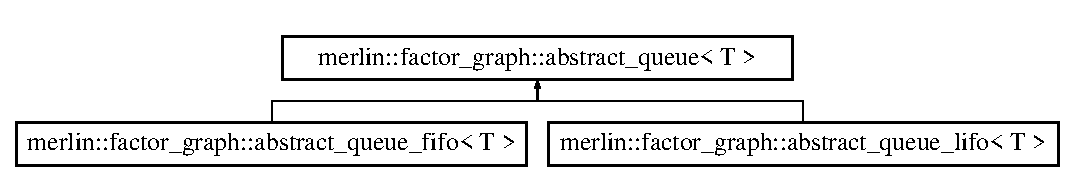
\includegraphics[height=1.992882cm]{classmerlin_1_1factor__graph_1_1abstract__queue}
\end{center}
\end{figure}


\subsection{Detailed Description}
\subsubsection*{template$<$class T$>$\\*
class merlin\+::factor\+\_\+graph\+::abstract\+\_\+queue$<$ T $>$}

Queue type wrapper. 

Definition at line 279 of file factor\+\_\+graph.\+h.



The documentation for this class was generated from the following file\+:\begin{DoxyCompactItemize}
\item 
src/include/\hyperlink{factor__graph_8h}{factor\+\_\+graph.\+h}\end{DoxyCompactItemize}

\hypertarget{classmerlin_1_1factor__graph_1_1abstract__queue__fifo}{}\section{merlin\+:\+:factor\+\_\+graph\+:\+:abstract\+\_\+queue\+\_\+fifo$<$ T $>$ Class Template Reference}
\label{classmerlin_1_1factor__graph_1_1abstract__queue__fifo}\index{merlin\+::factor\+\_\+graph\+::abstract\+\_\+queue\+\_\+fifo$<$ T $>$@{merlin\+::factor\+\_\+graph\+::abstract\+\_\+queue\+\_\+fifo$<$ T $>$}}


Queue type for breadth-\/first search.  




{\ttfamily \#include $<$factor\+\_\+graph.\+h$>$}

Inheritance diagram for merlin\+:\+:factor\+\_\+graph\+:\+:abstract\+\_\+queue\+\_\+fifo$<$ T $>$\+:\begin{figure}[H]
\begin{center}
\leavevmode
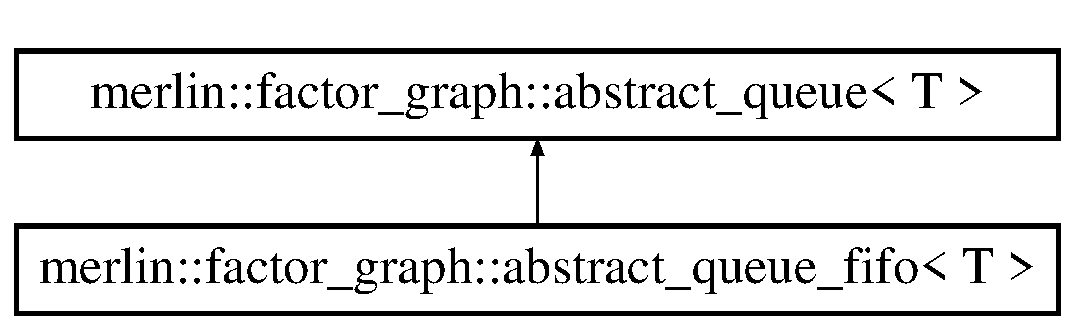
\includegraphics[height=2.000000cm]{classmerlin_1_1factor__graph_1_1abstract__queue__fifo}
\end{center}
\end{figure}


\subsection{Detailed Description}
\subsubsection*{template$<$class T$>$\\*
class merlin\+::factor\+\_\+graph\+::abstract\+\_\+queue\+\_\+fifo$<$ T $>$}

Queue type for breadth-\/first search. 

Definition at line 314 of file factor\+\_\+graph.\+h.



The documentation for this class was generated from the following file\+:\begin{DoxyCompactItemize}
\item 
src/include/\hyperlink{factor__graph_8h}{factor\+\_\+graph.\+h}\end{DoxyCompactItemize}

\hypertarget{classmerlin_1_1factor__graph_1_1abstract__queue__lifo}{}\section{merlin\+:\+:factor\+\_\+graph\+:\+:abstract\+\_\+queue\+\_\+lifo$<$ T $>$ Class Template Reference}
\label{classmerlin_1_1factor__graph_1_1abstract__queue__lifo}\index{merlin\+::factor\+\_\+graph\+::abstract\+\_\+queue\+\_\+lifo$<$ T $>$@{merlin\+::factor\+\_\+graph\+::abstract\+\_\+queue\+\_\+lifo$<$ T $>$}}


Stack type for depth-\/first search.  




{\ttfamily \#include $<$factor\+\_\+graph.\+h$>$}

Inheritance diagram for merlin\+:\+:factor\+\_\+graph\+:\+:abstract\+\_\+queue\+\_\+lifo$<$ T $>$\+:\begin{figure}[H]
\begin{center}
\leavevmode
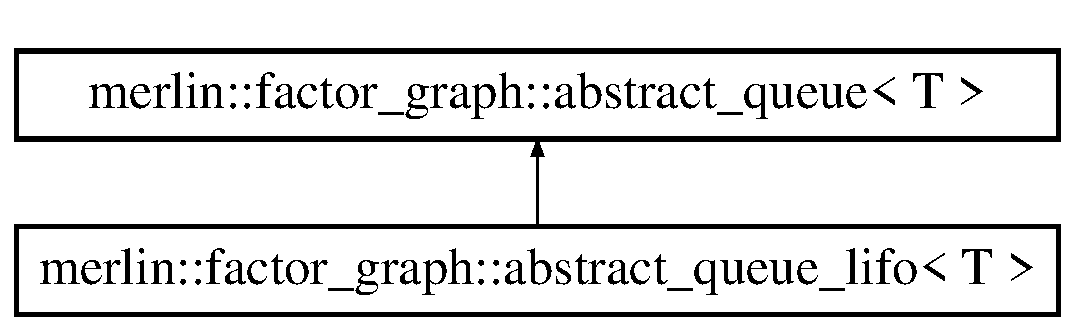
\includegraphics[height=2.000000cm]{classmerlin_1_1factor__graph_1_1abstract__queue__lifo}
\end{center}
\end{figure}


\subsection{Detailed Description}
\subsubsection*{template$<$class T$>$\\*
class merlin\+::factor\+\_\+graph\+::abstract\+\_\+queue\+\_\+lifo$<$ T $>$}

Stack type for depth-\/first search. 

Definition at line 293 of file factor\+\_\+graph.\+h.



The documentation for this class was generated from the following file\+:\begin{DoxyCompactItemize}
\item 
src/include/\hyperlink{factor__graph_8h}{factor\+\_\+graph.\+h}\end{DoxyCompactItemize}

\hypertarget{classmerlin_1_1algorithm}{}\section{merlin\+:\+:algorithm Class Reference}
\label{classmerlin_1_1algorithm}\index{merlin\+::algorithm@{merlin\+::algorithm}}


Interface for all inference algorithms.  




{\ttfamily \#include $<$algorithm.\+h$>$}

Inheritance diagram for merlin\+:\+:algorithm\+:\begin{figure}[H]
\begin{center}
\leavevmode
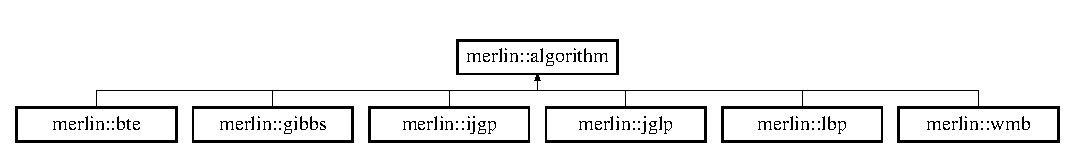
\includegraphics[height=1.681682cm]{classmerlin_1_1algorithm}
\end{center}
\end{figure}
\subsection*{Public Member Functions}
\begin{DoxyCompactItemize}
\item 
\hyperlink{classmerlin_1_1algorithm_adf0585fe727915bdae253d0213c0db80}{algorithm} ()\hypertarget{classmerlin_1_1algorithm_adf0585fe727915bdae253d0213c0db80}{}\label{classmerlin_1_1algorithm_adf0585fe727915bdae253d0213c0db80}

\begin{DoxyCompactList}\small\item\em Constructs an empty algorithm. \end{DoxyCompactList}\item 
virtual \hyperlink{classmerlin_1_1algorithm}{algorithm} $\ast$ \hyperlink{classmerlin_1_1algorithm_a10f787e24c1fd5ec92c26b18efb0b8db}{clone} () const =0
\begin{DoxyCompactList}\small\item\em Clone the current algorithm interface. \end{DoxyCompactList}\item 
virtual \hyperlink{classmerlin_1_1algorithm_a15a4cf8bb6ed1dc1de3a9e7383c2bbc1}{$\sim$algorithm} ()\hypertarget{classmerlin_1_1algorithm_a15a4cf8bb6ed1dc1de3a9e7383c2bbc1}{}\label{classmerlin_1_1algorithm_a15a4cf8bb6ed1dc1de3a9e7383c2bbc1}

\begin{DoxyCompactList}\small\item\em Destructs the algorithm. \end{DoxyCompactList}\item 
virtual void \hyperlink{classmerlin_1_1algorithm_af43f277863c17eeb153c652f9c3c54cd}{init} ()=0
\begin{DoxyCompactList}\small\item\em Inialize the algorithm. \end{DoxyCompactList}\item 
virtual void \hyperlink{classmerlin_1_1algorithm_a6a701ee51b3d1009041702129161b0de}{run} ()=0
\begin{DoxyCompactList}\small\item\em Run the algorithm. \end{DoxyCompactList}\item 
virtual double \hyperlink{classmerlin_1_1algorithm_a26eadf71ba80c0a9cd3d7cfe18c95717}{logZ} () const =0
\begin{DoxyCompactList}\small\item\em Log value of the partition function. \end{DoxyCompactList}\item 
virtual double \hyperlink{classmerlin_1_1algorithm_aeece2e8f008bcc94697353088c4afefe}{log\+Zub} () const =0
\begin{DoxyCompactList}\small\item\em Upper bound on the log partition function. \end{DoxyCompactList}\item 
virtual double \hyperlink{classmerlin_1_1algorithm_a14d163a3e90a898487d3a6e273e1fecf}{log\+Zlb} () const =0
\begin{DoxyCompactList}\small\item\em Lower bound on the log partition function. \end{DoxyCompactList}\item 
virtual double \hyperlink{classmerlin_1_1algorithm_a2698bb69f5559889d4903a640f08cd66}{ub} () const =0
\begin{DoxyCompactList}\small\item\em Upper bound on the optimal value. \end{DoxyCompactList}\item 
virtual double \hyperlink{classmerlin_1_1algorithm_adc3f19055c0466682b5577049df14863}{lb} () const =0
\begin{DoxyCompactList}\small\item\em Lower bound on the optimal value. \end{DoxyCompactList}\item 
virtual std\+::vector$<$ size\+\_\+t $>$ \hyperlink{classmerlin_1_1algorithm_a3d84d2595e6235db93a9bb3e1a012e48}{best\+\_\+config} () const =0
\begin{DoxyCompactList}\small\item\em Best configuration. \end{DoxyCompactList}\item 
virtual const \hyperlink{classmerlin_1_1factor}{factor} \& \hyperlink{classmerlin_1_1algorithm_a617b3e562037a7716f7cfd6cf1e55c19}{belief} (size\+\_\+t i) const =0
\begin{DoxyCompactList}\small\item\em Belief associated with a node of the graph. \end{DoxyCompactList}\item 
virtual const \hyperlink{classmerlin_1_1factor}{factor} \& \hyperlink{classmerlin_1_1algorithm_adc966d1ed7ac479754441bab138f7efa}{belief} (\hyperlink{classmerlin_1_1variable}{variable} v) const =0
\begin{DoxyCompactList}\small\item\em Belief associated with a particular variable. \end{DoxyCompactList}\item 
virtual const \hyperlink{classmerlin_1_1factor}{factor} \& \hyperlink{classmerlin_1_1algorithm_ad19b068623b85ad1cd4bb262e7bcfc6f}{belief} (\hyperlink{classmerlin_1_1variable__set}{variable\+\_\+set} vs) const =0
\begin{DoxyCompactList}\small\item\em Belief associated with a set of variables. \end{DoxyCompactList}\item 
virtual const std\+::vector$<$ \hyperlink{classmerlin_1_1factor}{factor} $>$ \& \hyperlink{classmerlin_1_1algorithm_a0b70d8fe87b32bca601a3d116b673b47}{beliefs} () const =0
\begin{DoxyCompactList}\small\item\em Beliefs associated with the variables. \end{DoxyCompactList}\item 
void \hyperlink{classmerlin_1_1algorithm_a5966656c44e83ffd5c77f40b507fcfc2}{set\+\_\+stop\+\_\+iter} (double d)
\begin{DoxyCompactList}\small\item\em Set the number of iterations. \end{DoxyCompactList}\item 
void \hyperlink{classmerlin_1_1algorithm_a14631bff623456c8f9e50cd54ea12bc0}{set\+\_\+stop\+\_\+obj} (double d)
\begin{DoxyCompactList}\small\item\em Set the minumum objective change before stopping. \end{DoxyCompactList}\item 
void \hyperlink{classmerlin_1_1algorithm_a9ec636be897b4ca62a3dc3bb493472e4}{set\+\_\+stop\+\_\+msg} (double d)
\begin{DoxyCompactList}\small\item\em Set the minimum ammount a message changes before stopping. \end{DoxyCompactList}\end{DoxyCompactItemize}
\subsection*{Protected Attributes}
\begin{DoxyCompactItemize}
\item 
double \hyperlink{classmerlin_1_1algorithm_a292ad6727f86126574943414afcd4196}{m\+\_\+stop\+\_\+iter}\hypertarget{classmerlin_1_1algorithm_a292ad6727f86126574943414afcd4196}{}\label{classmerlin_1_1algorithm_a292ad6727f86126574943414afcd4196}

\begin{DoxyCompactList}\small\item\em Stopping criteria (iterations) \end{DoxyCompactList}\item 
double \hyperlink{classmerlin_1_1algorithm_afe10662910ee8c4349a17684fd799a9b}{m\+\_\+stop\+\_\+obj}\hypertarget{classmerlin_1_1algorithm_afe10662910ee8c4349a17684fd799a9b}{}\label{classmerlin_1_1algorithm_afe10662910ee8c4349a17684fd799a9b}

\begin{DoxyCompactList}\small\item\em Stopping criteria (objective change) \end{DoxyCompactList}\item 
double \hyperlink{classmerlin_1_1algorithm_a3ad7c9e3331f03f7010e466da2e951dd}{m\+\_\+stop\+\_\+msg}\hypertarget{classmerlin_1_1algorithm_a3ad7c9e3331f03f7010e466da2e951dd}{}\label{classmerlin_1_1algorithm_a3ad7c9e3331f03f7010e466da2e951dd}

\begin{DoxyCompactList}\small\item\em Stopping criteria (message change) \end{DoxyCompactList}\item 
double \hyperlink{classmerlin_1_1algorithm_a8102421ee6a9ccc1378a808540613a4b}{m\+\_\+start\+\_\+time}\hypertarget{classmerlin_1_1algorithm_a8102421ee6a9ccc1378a808540613a4b}{}\label{classmerlin_1_1algorithm_a8102421ee6a9ccc1378a808540613a4b}

\begin{DoxyCompactList}\small\item\em Start time. \end{DoxyCompactList}\end{DoxyCompactItemize}


\subsection{Detailed Description}
Interface for all inference algorithms. 

The class provides the functional interface for any probabilistic inference algorithm. It is a pure virtual class and therefore it should be implemented by a concrete (derived) inference algorithm (e.\+g., wmb). 

Definition at line 47 of file algorithm.\+h.



\subsection{Member Function Documentation}
\index{merlin\+::algorithm@{merlin\+::algorithm}!belief@{belief}}
\index{belief@{belief}!merlin\+::algorithm@{merlin\+::algorithm}}
\subsubsection[{\texorpdfstring{belief(size\+\_\+t i) const =0}{belief(size_t i) const =0}}]{\setlength{\rightskip}{0pt plus 5cm}const {\bf factor} \& merlin\+::algorithm\+::belief (
\begin{DoxyParamCaption}
\item[{size\+\_\+t}]{i}
\end{DoxyParamCaption}
) const\hspace{0.3cm}{\ttfamily [pure virtual]}}\hypertarget{classmerlin_1_1algorithm_a617b3e562037a7716f7cfd6cf1e55c19}{}\label{classmerlin_1_1algorithm_a617b3e562037a7716f7cfd6cf1e55c19}


Belief associated with a node of the graph. 

\begin{DoxyReturn}{Returns}
the belief associated with a node of the graph. Nodes correspond typically to variables. The belied is a function represented by the Factor class. 
\end{DoxyReturn}

\begin{DoxyParams}{Parameters}
{\em i} & The index of the node in the graph (from 0) \\
\hline
\end{DoxyParams}


Implemented in \hyperlink{classmerlin_1_1gibbs_a578f69706383e3a29fabc65e8001b433}{merlin\+::gibbs}, \hyperlink{classmerlin_1_1ijgp_a43ba4b5f66a27881b8b6d4a0fed23b3f}{merlin\+::ijgp}, \hyperlink{classmerlin_1_1jglp_a75fe3423fa5f1d46f5878de99f732ed4}{merlin\+::jglp}, \hyperlink{classmerlin_1_1lbp_a1df7d0dc71990b595c1a169498a2e087}{merlin\+::lbp}, \hyperlink{classmerlin_1_1wmb_aeb4e3096861b442f85ad8d1344172d18}{merlin\+::wmb}, and \hyperlink{classmerlin_1_1bte_a8e08df0db094f22edd4067a6b78975bb}{merlin\+::bte}.



Referenced by $\sim$algorithm().

\index{merlin\+::algorithm@{merlin\+::algorithm}!belief@{belief}}
\index{belief@{belief}!merlin\+::algorithm@{merlin\+::algorithm}}
\subsubsection[{\texorpdfstring{belief(variable v) const =0}{belief(variable v) const =0}}]{\setlength{\rightskip}{0pt plus 5cm}virtual const {\bf factor}\& merlin\+::algorithm\+::belief (
\begin{DoxyParamCaption}
\item[{{\bf variable}}]{v}
\end{DoxyParamCaption}
) const\hspace{0.3cm}{\ttfamily [pure virtual]}}\hypertarget{classmerlin_1_1algorithm_adc966d1ed7ac479754441bab138f7efa}{}\label{classmerlin_1_1algorithm_adc966d1ed7ac479754441bab138f7efa}


Belief associated with a particular variable. 


\begin{DoxyParams}{Parameters}
{\em v} & The variable to compute the belief of \\
\hline
\end{DoxyParams}
\begin{DoxyReturn}{Returns}
the belief associated with a particular variable in the graphical model. The belief is a function represented by the Factor class. 
\end{DoxyReturn}


Implemented in \hyperlink{classmerlin_1_1gibbs_aea5e692a62aee1fff134398565e85c6e}{merlin\+::gibbs}, \hyperlink{classmerlin_1_1ijgp_a950771f418c3fa8980e449c1b081a9cc}{merlin\+::ijgp}, \hyperlink{classmerlin_1_1jglp_ab682129e900ebd41c44b0516e7997a9e}{merlin\+::jglp}, \hyperlink{classmerlin_1_1lbp_af34aa24b4de8a0ae9f579ba6d83ee0bf}{merlin\+::lbp}, \hyperlink{classmerlin_1_1wmb_a93588ec46d0cc1e54179ce8555862941}{merlin\+::wmb}, and \hyperlink{classmerlin_1_1bte_acead5460cd29483aa0736a6aca0e73d3}{merlin\+::bte}.

\index{merlin\+::algorithm@{merlin\+::algorithm}!belief@{belief}}
\index{belief@{belief}!merlin\+::algorithm@{merlin\+::algorithm}}
\subsubsection[{\texorpdfstring{belief(variable\+\_\+set vs) const =0}{belief(variable_set vs) const =0}}]{\setlength{\rightskip}{0pt plus 5cm}virtual const {\bf factor}\& merlin\+::algorithm\+::belief (
\begin{DoxyParamCaption}
\item[{{\bf variable\+\_\+set}}]{vs}
\end{DoxyParamCaption}
) const\hspace{0.3cm}{\ttfamily [pure virtual]}}\hypertarget{classmerlin_1_1algorithm_ad19b068623b85ad1cd4bb262e7bcfc6f}{}\label{classmerlin_1_1algorithm_ad19b068623b85ad1cd4bb262e7bcfc6f}


Belief associated with a set of variables. 


\begin{DoxyParams}{Parameters}
{\em vs} & The set of variables to compute the belief of \\
\hline
\end{DoxyParams}
\begin{DoxyReturn}{Returns}
the belief associated with a set of variables in the graphical model. The belief is a function represented by the Factor class. 
\end{DoxyReturn}


Implemented in \hyperlink{classmerlin_1_1gibbs_af8b834f1ca8b2775a2a896b32442e303}{merlin\+::gibbs}, \hyperlink{classmerlin_1_1ijgp_a5506025b0268f56419a472d674faa476}{merlin\+::ijgp}, \hyperlink{classmerlin_1_1jglp_abc9393073179fadfd12999faea87a62c}{merlin\+::jglp}, \hyperlink{classmerlin_1_1lbp_a37223c0f6db663160062bed87d2ac803}{merlin\+::lbp}, \hyperlink{classmerlin_1_1wmb_afe50fb8a9334a9f8b4653a75f20abd30}{merlin\+::wmb}, and \hyperlink{classmerlin_1_1bte_af18f05f849f6fd0efadfd98735aac98c}{merlin\+::bte}.

\index{merlin\+::algorithm@{merlin\+::algorithm}!beliefs@{beliefs}}
\index{beliefs@{beliefs}!merlin\+::algorithm@{merlin\+::algorithm}}
\subsubsection[{\texorpdfstring{beliefs() const =0}{beliefs() const =0}}]{\setlength{\rightskip}{0pt plus 5cm}const std\+::vector$<$ Factor $>$ \& merlin\+::algorithm\+::beliefs (
\begin{DoxyParamCaption}
{}
\end{DoxyParamCaption}
) const\hspace{0.3cm}{\ttfamily [pure virtual]}}\hypertarget{classmerlin_1_1algorithm_a0b70d8fe87b32bca601a3d116b673b47}{}\label{classmerlin_1_1algorithm_a0b70d8fe87b32bca601a3d116b673b47}


Beliefs associated with the variables. 

\begin{DoxyReturn}{Returns}
the beliefs associated with the variables in the graphical model (one belief for each of the variables). The output vector is indexed by the same indexes used for the variables. 
\end{DoxyReturn}


Implemented in \hyperlink{classmerlin_1_1gibbs_aae4b98aa02e5483d04fed2d9046c0900}{merlin\+::gibbs}, \hyperlink{classmerlin_1_1ijgp_a031930b83efb5b52a5af5387a18ee0e2}{merlin\+::ijgp}, \hyperlink{classmerlin_1_1jglp_a44be9483e6b79d87f70fd7c893d8f70a}{merlin\+::jglp}, \hyperlink{classmerlin_1_1lbp_adccd484965707ae36ffc7f1d49b58ac9}{merlin\+::lbp}, \hyperlink{classmerlin_1_1wmb_ab433dc54ee1777fa163af30aa71bde3d}{merlin\+::wmb}, and \hyperlink{classmerlin_1_1bte_a4a10aa68792892ac1d6ab9c8ccfcf44e}{merlin\+::bte}.



Referenced by $\sim$algorithm().

\index{merlin\+::algorithm@{merlin\+::algorithm}!best\+\_\+config@{best\+\_\+config}}
\index{best\+\_\+config@{best\+\_\+config}!merlin\+::algorithm@{merlin\+::algorithm}}
\subsubsection[{\texorpdfstring{best\+\_\+config() const =0}{best_config() const =0}}]{\setlength{\rightskip}{0pt plus 5cm}virtual std\+::vector$<$size\+\_\+t$>$ merlin\+::algorithm\+::best\+\_\+config (
\begin{DoxyParamCaption}
{}
\end{DoxyParamCaption}
) const\hspace{0.3cm}{\ttfamily [pure virtual]}}\hypertarget{classmerlin_1_1algorithm_a3d84d2595e6235db93a9bb3e1a012e48}{}\label{classmerlin_1_1algorithm_a3d84d2595e6235db93a9bb3e1a012e48}


Best configuration. 

\begin{DoxyReturn}{Returns}
a vector containing the best configuration of the variables (i.\+e., variable value assignments) found so far. It is specific to optimization tasks (e.\+g., M\+AP, Marginal M\+AP). 
\end{DoxyReturn}


Implemented in \hyperlink{classmerlin_1_1gibbs_a10fd6e4e76f510f10a802e97584aff9e}{merlin\+::gibbs}, \hyperlink{classmerlin_1_1lbp_a7511d2d8fe99649f85a5c8ae88a8a379}{merlin\+::lbp}, \hyperlink{classmerlin_1_1ijgp_af54b5585c353a821071a1ac1f0570679}{merlin\+::ijgp}, \hyperlink{classmerlin_1_1jglp_a4e7ff17be5074ce9010fda0154f81fbf}{merlin\+::jglp}, \hyperlink{classmerlin_1_1bte_a09a23c8791601d912bf6872f0b13510a}{merlin\+::bte}, and \hyperlink{classmerlin_1_1wmb_ae2de6f3bc30e524b6e9190d02631af4f}{merlin\+::wmb}.



Referenced by $\sim$algorithm().

\index{merlin\+::algorithm@{merlin\+::algorithm}!clone@{clone}}
\index{clone@{clone}!merlin\+::algorithm@{merlin\+::algorithm}}
\subsubsection[{\texorpdfstring{clone() const =0}{clone() const =0}}]{\setlength{\rightskip}{0pt plus 5cm}virtual {\bf algorithm}$\ast$ merlin\+::algorithm\+::clone (
\begin{DoxyParamCaption}
{}
\end{DoxyParamCaption}
) const\hspace{0.3cm}{\ttfamily [pure virtual]}}\hypertarget{classmerlin_1_1algorithm_a10f787e24c1fd5ec92c26b18efb0b8db}{}\label{classmerlin_1_1algorithm_a10f787e24c1fd5ec92c26b18efb0b8db}


Clone the current algorithm interface. 

\begin{DoxyReturn}{Returns}
a pointer to the object storing the copy of the algorithm. 
\end{DoxyReturn}


Implemented in \hyperlink{classmerlin_1_1lbp_a4d2e317106a40ca49074f898a7a46fb0}{merlin\+::lbp}, \hyperlink{classmerlin_1_1ijgp_af3ecb1e386de25e892d3246e9fd14a1e}{merlin\+::ijgp}, \hyperlink{classmerlin_1_1jglp_af6e5931262caafec1aab81f6d3001419}{merlin\+::jglp}, \hyperlink{classmerlin_1_1bte_a074c1b194629f26df5a5d99102a20108}{merlin\+::bte}, \hyperlink{classmerlin_1_1wmb_a9a9120ce51df90d8c6fc60c01f308dd4}{merlin\+::wmb}, and \hyperlink{classmerlin_1_1gibbs_a3479cca656a53a22c32ecdaa1a010308}{merlin\+::gibbs}.



Referenced by algorithm().

\index{merlin\+::algorithm@{merlin\+::algorithm}!init@{init}}
\index{init@{init}!merlin\+::algorithm@{merlin\+::algorithm}}
\subsubsection[{\texorpdfstring{init()=0}{init()=0}}]{\setlength{\rightskip}{0pt plus 5cm}virtual void merlin\+::algorithm\+::init (
\begin{DoxyParamCaption}
{}
\end{DoxyParamCaption}
)\hspace{0.3cm}{\ttfamily [pure virtual]}}\hypertarget{classmerlin_1_1algorithm_af43f277863c17eeb153c652f9c3c54cd}{}\label{classmerlin_1_1algorithm_af43f277863c17eeb153c652f9c3c54cd}


Inialize the algorithm. 

The initialization step must be performed before running the algorithm. 

Implemented in \hyperlink{classmerlin_1_1wmb_ac9a83bcbef3f06a48d6cd9bea8ad3ce6}{merlin\+::wmb}, \hyperlink{classmerlin_1_1ijgp_a8300ed201011020d5dffe498d3de44c1}{merlin\+::ijgp}, \hyperlink{classmerlin_1_1bte_aff473532708590dd696a6fd40d9d62e8}{merlin\+::bte}, \hyperlink{classmerlin_1_1jglp_a834f4f3ac58d3286843ed1e1fb8552dc}{merlin\+::jglp}, \hyperlink{classmerlin_1_1lbp_a61e6c00e8236acc65b59194e09180692}{merlin\+::lbp}, and \hyperlink{classmerlin_1_1gibbs_ac14684f895fc27b59f318632a786acb7}{merlin\+::gibbs}.



Referenced by $\sim$algorithm().

\index{merlin\+::algorithm@{merlin\+::algorithm}!lb@{lb}}
\index{lb@{lb}!merlin\+::algorithm@{merlin\+::algorithm}}
\subsubsection[{\texorpdfstring{lb() const =0}{lb() const =0}}]{\setlength{\rightskip}{0pt plus 5cm}virtual double merlin\+::algorithm\+::lb (
\begin{DoxyParamCaption}
{}
\end{DoxyParamCaption}
) const\hspace{0.3cm}{\ttfamily [pure virtual]}}\hypertarget{classmerlin_1_1algorithm_adc3f19055c0466682b5577049df14863}{}\label{classmerlin_1_1algorithm_adc3f19055c0466682b5577049df14863}


Lower bound on the optimal value. 

\begin{DoxyReturn}{Returns}
a lower bound on the optimal value defined by the inference task if available. 
\end{DoxyReturn}


Implemented in \hyperlink{classmerlin_1_1gibbs_a560e770c1d7fe247e5fcb088cd00198c}{merlin\+::gibbs}, \hyperlink{classmerlin_1_1lbp_af7cec119584c4ca671a82e23ac5098f1}{merlin\+::lbp}, \hyperlink{classmerlin_1_1ijgp_ae4313682960f210fc937627446fb70cf}{merlin\+::ijgp}, \hyperlink{classmerlin_1_1jglp_a56a4aa254f07ee4a651bf343ee14d63b}{merlin\+::jglp}, \hyperlink{classmerlin_1_1bte_ac0302ea356a59d0890e8a049c54841c0}{merlin\+::bte}, and \hyperlink{classmerlin_1_1wmb_a88a812b53de1bde731d7d21305be6041}{merlin\+::wmb}.



Referenced by $\sim$algorithm().

\index{merlin\+::algorithm@{merlin\+::algorithm}!logZ@{logZ}}
\index{logZ@{logZ}!merlin\+::algorithm@{merlin\+::algorithm}}
\subsubsection[{\texorpdfstring{log\+Z() const =0}{logZ() const =0}}]{\setlength{\rightskip}{0pt plus 5cm}virtual double merlin\+::algorithm\+::logZ (
\begin{DoxyParamCaption}
{}
\end{DoxyParamCaption}
) const\hspace{0.3cm}{\ttfamily [pure virtual]}}\hypertarget{classmerlin_1_1algorithm_a26eadf71ba80c0a9cd3d7cfe18c95717}{}\label{classmerlin_1_1algorithm_a26eadf71ba80c0a9cd3d7cfe18c95717}


Log value of the partition function. 

\begin{DoxyReturn}{Returns}
an estimate the log parition function. If the inference algorithm is an exact one then the return value is the exact log value of the partition function. 
\end{DoxyReturn}


Implemented in \hyperlink{classmerlin_1_1gibbs_a2a57b5f7fa9571060e134164ca39c68f}{merlin\+::gibbs}, \hyperlink{classmerlin_1_1lbp_a5f0f0d6b2605e1b3f47b6de9875d5590}{merlin\+::lbp}, \hyperlink{classmerlin_1_1ijgp_afb334bdd8a981984f1f97ce0d5c58bed}{merlin\+::ijgp}, \hyperlink{classmerlin_1_1jglp_a2a6a565403cbddd77109a3a6f85e3d35}{merlin\+::jglp}, \hyperlink{classmerlin_1_1bte_aa57126509e1c91198c21a01854787afa}{merlin\+::bte}, and \hyperlink{classmerlin_1_1wmb_aa2af3a4102ee07f954d24c44066f6a08}{merlin\+::wmb}.



Referenced by $\sim$algorithm().

\index{merlin\+::algorithm@{merlin\+::algorithm}!log\+Zlb@{log\+Zlb}}
\index{log\+Zlb@{log\+Zlb}!merlin\+::algorithm@{merlin\+::algorithm}}
\subsubsection[{\texorpdfstring{log\+Zlb() const =0}{logZlb() const =0}}]{\setlength{\rightskip}{0pt plus 5cm}virtual double merlin\+::algorithm\+::log\+Zlb (
\begin{DoxyParamCaption}
{}
\end{DoxyParamCaption}
) const\hspace{0.3cm}{\ttfamily [pure virtual]}}\hypertarget{classmerlin_1_1algorithm_a14d163a3e90a898487d3a6e273e1fecf}{}\label{classmerlin_1_1algorithm_a14d163a3e90a898487d3a6e273e1fecf}


Lower bound on the log partition function. 

\begin{DoxyReturn}{Returns}
a lower bound on the log value of the parition function. 
\end{DoxyReturn}


Implemented in \hyperlink{classmerlin_1_1gibbs_ab4ee1ac60166f1e30b14e07a534aa4b8}{merlin\+::gibbs}, \hyperlink{classmerlin_1_1lbp_ada4dd7a71b8ac11ad419f3f7b1b6d658}{merlin\+::lbp}, \hyperlink{classmerlin_1_1ijgp_aa19a722eda63c9471795aff804985d4e}{merlin\+::ijgp}, \hyperlink{classmerlin_1_1jglp_a53e258c9ac8e80e2a99019f350fafe23}{merlin\+::jglp}, \hyperlink{classmerlin_1_1bte_ae3c26e3c8aedeb945f5efc78046932fb}{merlin\+::bte}, and \hyperlink{classmerlin_1_1wmb_affa03e963d632f43e2c5967cd3f7bff4}{merlin\+::wmb}.



Referenced by $\sim$algorithm().

\index{merlin\+::algorithm@{merlin\+::algorithm}!log\+Zub@{log\+Zub}}
\index{log\+Zub@{log\+Zub}!merlin\+::algorithm@{merlin\+::algorithm}}
\subsubsection[{\texorpdfstring{log\+Zub() const =0}{logZub() const =0}}]{\setlength{\rightskip}{0pt plus 5cm}virtual double merlin\+::algorithm\+::log\+Zub (
\begin{DoxyParamCaption}
{}
\end{DoxyParamCaption}
) const\hspace{0.3cm}{\ttfamily [pure virtual]}}\hypertarget{classmerlin_1_1algorithm_aeece2e8f008bcc94697353088c4afefe}{}\label{classmerlin_1_1algorithm_aeece2e8f008bcc94697353088c4afefe}


Upper bound on the log partition function. 

\begin{DoxyReturn}{Returns}
an upper bound on the log value of the parition function. Most inference algorithms implemented in merlin support upper bounds on the log partition function. 
\end{DoxyReturn}


Implemented in \hyperlink{classmerlin_1_1gibbs_abfd6c9073faa8827b87acf333de77cd6}{merlin\+::gibbs}, \hyperlink{classmerlin_1_1lbp_a0451118b6fa2c1017512879e025afd4d}{merlin\+::lbp}, \hyperlink{classmerlin_1_1ijgp_ac0851bfb0a95f0a8ff4b00af298bf743}{merlin\+::ijgp}, \hyperlink{classmerlin_1_1jglp_a6f964c4acb649a3bf24bd46e8c414113}{merlin\+::jglp}, \hyperlink{classmerlin_1_1bte_a78cf8295cf726052647de96a8dec59ad}{merlin\+::bte}, and \hyperlink{classmerlin_1_1wmb_a91015e29caed663c30bb37cbd0609e24}{merlin\+::wmb}.



Referenced by $\sim$algorithm().

\index{merlin\+::algorithm@{merlin\+::algorithm}!run@{run}}
\index{run@{run}!merlin\+::algorithm@{merlin\+::algorithm}}
\subsubsection[{\texorpdfstring{run()=0}{run()=0}}]{\setlength{\rightskip}{0pt plus 5cm}virtual void merlin\+::algorithm\+::run (
\begin{DoxyParamCaption}
{}
\end{DoxyParamCaption}
)\hspace{0.3cm}{\ttfamily [pure virtual]}}\hypertarget{classmerlin_1_1algorithm_a6a701ee51b3d1009041702129161b0de}{}\label{classmerlin_1_1algorithm_a6a701ee51b3d1009041702129161b0de}


Run the algorithm. 

Solves a probabilistic inference task. 

Implemented in \hyperlink{classmerlin_1_1jglp_aa748730ca6abbe2359fb2497da674fb8}{merlin\+::jglp}, \hyperlink{classmerlin_1_1lbp_afa31a31b0cfd63590d57cb453a6ab751}{merlin\+::lbp}, \hyperlink{classmerlin_1_1wmb_acdbdfbded7a99152f8e7215c57cf1ab5}{merlin\+::wmb}, \hyperlink{classmerlin_1_1bte_a4ac6d3a739619c5066ffe9cfdfb8aaaf}{merlin\+::bte}, \hyperlink{classmerlin_1_1ijgp_ac255c416a80f2bddab2855e5f66df8bd}{merlin\+::ijgp}, and \hyperlink{classmerlin_1_1gibbs_a2f9555aa3830e21e15a74c2ce7dc2109}{merlin\+::gibbs}.



Referenced by $\sim$algorithm().

\index{merlin\+::algorithm@{merlin\+::algorithm}!set\+\_\+stop\+\_\+iter@{set\+\_\+stop\+\_\+iter}}
\index{set\+\_\+stop\+\_\+iter@{set\+\_\+stop\+\_\+iter}!merlin\+::algorithm@{merlin\+::algorithm}}
\subsubsection[{\texorpdfstring{set\+\_\+stop\+\_\+iter(double d)}{set_stop_iter(double d)}}]{\setlength{\rightskip}{0pt plus 5cm}void merlin\+::algorithm\+::set\+\_\+stop\+\_\+iter (
\begin{DoxyParamCaption}
\item[{double}]{d}
\end{DoxyParamCaption}
)\hspace{0.3cm}{\ttfamily [inline]}}\hypertarget{classmerlin_1_1algorithm_a5966656c44e83ffd5c77f40b507fcfc2}{}\label{classmerlin_1_1algorithm_a5966656c44e83ffd5c77f40b507fcfc2}


Set the number of iterations. 

Stop when d$\ast$(\# factors) updates have been done. 

Definition at line 188 of file algorithm.\+h.



References m\+\_\+stop\+\_\+iter.



Referenced by merlin\+::lbp\+::set\+\_\+properties().

\index{merlin\+::algorithm@{merlin\+::algorithm}!set\+\_\+stop\+\_\+msg@{set\+\_\+stop\+\_\+msg}}
\index{set\+\_\+stop\+\_\+msg@{set\+\_\+stop\+\_\+msg}!merlin\+::algorithm@{merlin\+::algorithm}}
\subsubsection[{\texorpdfstring{set\+\_\+stop\+\_\+msg(double d)}{set_stop_msg(double d)}}]{\setlength{\rightskip}{0pt plus 5cm}void merlin\+::algorithm\+::set\+\_\+stop\+\_\+msg (
\begin{DoxyParamCaption}
\item[{double}]{d}
\end{DoxyParamCaption}
)\hspace{0.3cm}{\ttfamily [inline]}}\hypertarget{classmerlin_1_1algorithm_a9ec636be897b4ca62a3dc3bb493472e4}{}\label{classmerlin_1_1algorithm_a9ec636be897b4ca62a3dc3bb493472e4}


Set the minimum ammount a message changes before stopping. 

Stop when message updates are less than {\itshape d}. 
\begin{DoxyParams}{Parameters}
{\em d} & The tolerated message update \\
\hline
\end{DoxyParams}


Definition at line 208 of file algorithm.\+h.



References m\+\_\+stop\+\_\+msg.



Referenced by merlin\+::lbp\+::set\+\_\+properties().

\index{merlin\+::algorithm@{merlin\+::algorithm}!set\+\_\+stop\+\_\+obj@{set\+\_\+stop\+\_\+obj}}
\index{set\+\_\+stop\+\_\+obj@{set\+\_\+stop\+\_\+obj}!merlin\+::algorithm@{merlin\+::algorithm}}
\subsubsection[{\texorpdfstring{set\+\_\+stop\+\_\+obj(double d)}{set_stop_obj(double d)}}]{\setlength{\rightskip}{0pt plus 5cm}void merlin\+::algorithm\+::set\+\_\+stop\+\_\+obj (
\begin{DoxyParamCaption}
\item[{double}]{d}
\end{DoxyParamCaption}
)\hspace{0.3cm}{\ttfamily [inline]}}\hypertarget{classmerlin_1_1algorithm_a14631bff623456c8f9e50cd54ea12bc0}{}\label{classmerlin_1_1algorithm_a14631bff623456c8f9e50cd54ea12bc0}


Set the minumum objective change before stopping. 

Stop when objective change is less than {\itshape d}. 
\begin{DoxyParams}{Parameters}
{\em d} & The objective change \\
\hline
\end{DoxyParams}


Definition at line 198 of file algorithm.\+h.



References m\+\_\+stop\+\_\+obj.



Referenced by merlin\+::lbp\+::set\+\_\+properties().

\index{merlin\+::algorithm@{merlin\+::algorithm}!ub@{ub}}
\index{ub@{ub}!merlin\+::algorithm@{merlin\+::algorithm}}
\subsubsection[{\texorpdfstring{ub() const =0}{ub() const =0}}]{\setlength{\rightskip}{0pt plus 5cm}virtual double merlin\+::algorithm\+::ub (
\begin{DoxyParamCaption}
{}
\end{DoxyParamCaption}
) const\hspace{0.3cm}{\ttfamily [pure virtual]}}\hypertarget{classmerlin_1_1algorithm_a2698bb69f5559889d4903a640f08cd66}{}\label{classmerlin_1_1algorithm_a2698bb69f5559889d4903a640f08cd66}


Upper bound on the optimal value. 

\begin{DoxyReturn}{Returns}
an upper bound on the optimal value defined by the inference task. It is specific to optimization tasks such as M\+AP and Marginal M\+AP inference. 
\end{DoxyReturn}


Implemented in \hyperlink{classmerlin_1_1gibbs_ac433bf8d912355ed96f4d2299f8d71d9}{merlin\+::gibbs}, \hyperlink{classmerlin_1_1lbp_a6f47094c1dd1b721c8b55b2a104bf708}{merlin\+::lbp}, \hyperlink{classmerlin_1_1ijgp_aa5813f62d79f2a2c2fcdb24cbc967040}{merlin\+::ijgp}, \hyperlink{classmerlin_1_1jglp_aeb00e60c9df427722f2ff791bdd056d9}{merlin\+::jglp}, \hyperlink{classmerlin_1_1bte_a8855426f65d43e799053282369728736}{merlin\+::bte}, and \hyperlink{classmerlin_1_1wmb_a78d08bbf18835324d79a4f73eebeecc7}{merlin\+::wmb}.



Referenced by $\sim$algorithm().



The documentation for this class was generated from the following file\+:\begin{DoxyCompactItemize}
\item 
src/include/\hyperlink{algorithm_8h}{algorithm.\+h}\end{DoxyCompactItemize}

\hypertarget{structmerlin_1_1factor_1_1binOpDivide}{}\section{merlin\+:\+:factor\+:\+:bin\+Op\+Divide Struct Reference}
\label{structmerlin_1_1factor_1_1binOpDivide}\index{merlin\+::factor\+::bin\+Op\+Divide@{merlin\+::factor\+::bin\+Op\+Divide}}


Functor for binary operation / (division) on the factor table.  




{\ttfamily \#include $<$factor.\+h$>$}



\subsection{Detailed Description}
Functor for binary operation / (division) on the factor table. 

Definition at line 745 of file factor.\+h.



The documentation for this struct was generated from the following file\+:\begin{DoxyCompactItemize}
\item 
src/include/\hyperlink{factor_8h}{factor.\+h}\end{DoxyCompactItemize}

\hypertarget{structmerlin_1_1factor_1_1binOpMinus}{}\section{merlin\+:\+:factor\+:\+:bin\+Op\+Minus Struct Reference}
\label{structmerlin_1_1factor_1_1binOpMinus}\index{merlin\+::factor\+::bin\+Op\+Minus@{merlin\+::factor\+::bin\+Op\+Minus}}


Functor for binary operation -\/ (substraction) on the factor table.  




{\ttfamily \#include $<$factor.\+h$>$}



\subsection{Detailed Description}
Functor for binary operation -\/ (substraction) on the factor table. 

Definition at line 715 of file factor.\+h.



The documentation for this struct was generated from the following file\+:\begin{DoxyCompactItemize}
\item 
src/include/\hyperlink{factor_8h}{factor.\+h}\end{DoxyCompactItemize}

\hypertarget{structmerlin_1_1factor_1_1binOpPlus}{}\section{merlin\+:\+:factor\+:\+:bin\+Op\+Plus Struct Reference}
\label{structmerlin_1_1factor_1_1binOpPlus}\index{merlin\+::factor\+::bin\+Op\+Plus@{merlin\+::factor\+::bin\+Op\+Plus}}


Functor for binary operation + (summation) on the factor table.  




{\ttfamily \#include $<$factor.\+h$>$}



\subsection{Detailed Description}
Functor for binary operation + (summation) on the factor table. 

Definition at line 701 of file factor.\+h.



The documentation for this struct was generated from the following file\+:\begin{DoxyCompactItemize}
\item 
src/include/\hyperlink{factor_8h}{factor.\+h}\end{DoxyCompactItemize}

\hypertarget{structmerlin_1_1factor_1_1binOpPower}{}\section{merlin\+:\+:factor\+:\+:bin\+Op\+Power Struct Reference}
\label{structmerlin_1_1factor_1_1binOpPower}\index{merlin\+::factor\+::bin\+Op\+Power@{merlin\+::factor\+::bin\+Op\+Power}}


Functor for binary operation $^\wedge$ (power) on the factor table.  




{\ttfamily \#include $<$factor.\+h$>$}



\subsection{Detailed Description}
Functor for binary operation $^\wedge$ (power) on the factor table. 

Definition at line 759 of file factor.\+h.



The documentation for this struct was generated from the following file\+:\begin{DoxyCompactItemize}
\item 
src/include/\hyperlink{factor_8h}{factor.\+h}\end{DoxyCompactItemize}

\hypertarget{structmerlin_1_1factor_1_1binOpTimes}{}\section{merlin\+:\+:factor\+:\+:bin\+Op\+Times Struct Reference}
\label{structmerlin_1_1factor_1_1binOpTimes}\index{merlin\+::factor\+::bin\+Op\+Times@{merlin\+::factor\+::bin\+Op\+Times}}


Functor for binary operation $\ast$ (multiplication) on the factor table.  




{\ttfamily \#include $<$factor.\+h$>$}



\subsection{Detailed Description}
Functor for binary operation $\ast$ (multiplication) on the factor table. 

Definition at line 731 of file factor.\+h.



The documentation for this struct was generated from the following file\+:\begin{DoxyCompactItemize}
\item 
src/include/\hyperlink{factor_8h}{factor.\+h}\end{DoxyCompactItemize}

\hypertarget{classmerlin_1_1bte}{}\section{merlin\+:\+:bte Class Reference}
\label{classmerlin_1_1bte}\index{merlin\+::bte@{merlin\+::bte}}


{\ttfamily \#include $<$bte.\+h$>$}

Inheritance diagram for merlin\+:\+:bte\+:\begin{figure}[H]
\begin{center}
\leavevmode
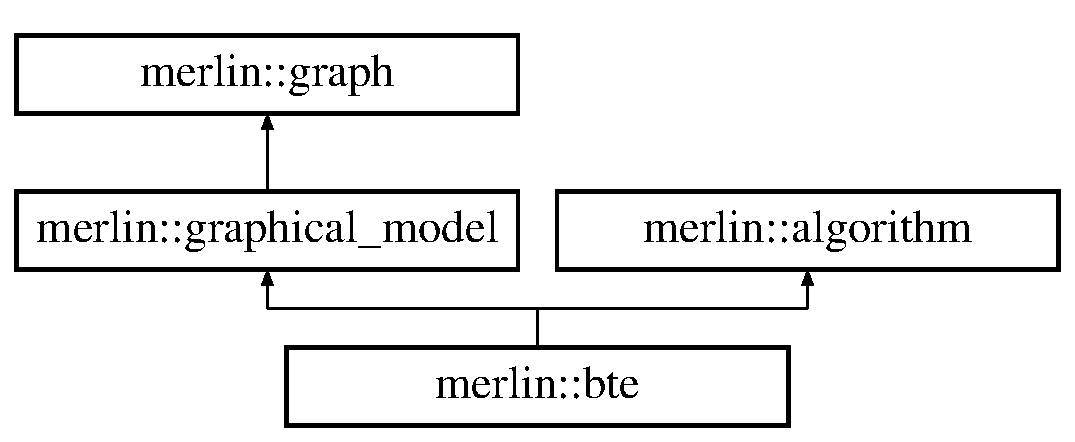
\includegraphics[height=3.000000cm]{classmerlin_1_1bte}
\end{center}
\end{figure}
\subsection*{Public Types}
\begin{DoxyCompactItemize}
\item 
typedef \hyperlink{classmerlin_1_1graphical__model_ab2b46f09d8142bb68f243ecadbdabb6b}{graphical\+\_\+model\+::findex} \hyperlink{classmerlin_1_1bte_a9a8220f4a0d833a5b0044a05aecf21d3}{findex}\hypertarget{classmerlin_1_1bte_a9a8220f4a0d833a5b0044a05aecf21d3}{}\label{classmerlin_1_1bte_a9a8220f4a0d833a5b0044a05aecf21d3}

\begin{DoxyCompactList}\small\item\em Factor index. \end{DoxyCompactList}\item 
typedef \hyperlink{classmerlin_1_1graphical__model_a275006a490bc09239c12a4d93d53b135}{graphical\+\_\+model\+::vindex} \hyperlink{classmerlin_1_1bte_afd42180c7906586fb39a0384d096fa4a}{vindex}\hypertarget{classmerlin_1_1bte_afd42180c7906586fb39a0384d096fa4a}{}\label{classmerlin_1_1bte_afd42180c7906586fb39a0384d096fa4a}

\begin{DoxyCompactList}\small\item\em Variable index. \end{DoxyCompactList}\item 
typedef \hyperlink{classmerlin_1_1graphical__model_a615e25ec6594615fddfd4c3c4776b99f}{graphical\+\_\+model\+::flist} \hyperlink{classmerlin_1_1bte_a5152e6b6f4f04d615bf911fcfe92676f}{flist}\hypertarget{classmerlin_1_1bte_a5152e6b6f4f04d615bf911fcfe92676f}{}\label{classmerlin_1_1bte_a5152e6b6f4f04d615bf911fcfe92676f}

\begin{DoxyCompactList}\small\item\em Collection of factor indices. \end{DoxyCompactList}\end{DoxyCompactItemize}
\subsection*{Public Member Functions}
\begin{DoxyCompactItemize}
\item 
\hyperlink{classmerlin_1_1bte_a711d5860e89aaeab8110f915fe75921e}{bte} ()\hypertarget{classmerlin_1_1bte_a711d5860e89aaeab8110f915fe75921e}{}\label{classmerlin_1_1bte_a711d5860e89aaeab8110f915fe75921e}

\begin{DoxyCompactList}\small\item\em Default constructor. \end{DoxyCompactList}\item 
\hyperlink{classmerlin_1_1bte_aa916d19b34aa1bfccde81b14b306b5a3}{bte} (const \hyperlink{classmerlin_1_1graphical__model}{graphical\+\_\+model} \&gm)\hypertarget{classmerlin_1_1bte_aa916d19b34aa1bfccde81b14b306b5a3}{}\label{classmerlin_1_1bte_aa916d19b34aa1bfccde81b14b306b5a3}

\begin{DoxyCompactList}\small\item\em Constructor with a graphical model. \end{DoxyCompactList}\item 
virtual \hyperlink{classmerlin_1_1bte}{bte} $\ast$ \hyperlink{classmerlin_1_1bte_a074c1b194629f26df5a5d99102a20108}{clone} () const 
\begin{DoxyCompactList}\small\item\em Clone the algorithm. \end{DoxyCompactList}\item 
double \hyperlink{classmerlin_1_1bte_a8855426f65d43e799053282369728736}{ub} () const 
\begin{DoxyCompactList}\small\item\em Upper bound on the optimal value. \end{DoxyCompactList}\item 
double \hyperlink{classmerlin_1_1bte_ac0302ea356a59d0890e8a049c54841c0}{lb} () const 
\begin{DoxyCompactList}\small\item\em Lower bound on the optimal value. \end{DoxyCompactList}\item 
std\+::vector$<$ size\+\_\+t $>$ \hyperlink{classmerlin_1_1bte_a09a23c8791601d912bf6872f0b13510a}{best\+\_\+config} () const 
\begin{DoxyCompactList}\small\item\em Best configuration. \end{DoxyCompactList}\item 
double \hyperlink{classmerlin_1_1bte_aa57126509e1c91198c21a01854787afa}{logZ} () const 
\begin{DoxyCompactList}\small\item\em Log value of the partition function. \end{DoxyCompactList}\item 
double \hyperlink{classmerlin_1_1bte_a78cf8295cf726052647de96a8dec59ad}{log\+Zub} () const 
\begin{DoxyCompactList}\small\item\em Upper bound on the log partition function. \end{DoxyCompactList}\item 
double \hyperlink{classmerlin_1_1bte_ae3c26e3c8aedeb945f5efc78046932fb}{log\+Zlb} () const 
\begin{DoxyCompactList}\small\item\em Lower bound on the log partition function. \end{DoxyCompactList}\item 
const \hyperlink{classmerlin_1_1factor}{factor} \& \hyperlink{classmerlin_1_1bte_a8e08df0db094f22edd4067a6b78975bb}{belief} (size\+\_\+t f) const 
\begin{DoxyCompactList}\small\item\em Belief associated with a node of the graph. \end{DoxyCompactList}\item 
const \hyperlink{classmerlin_1_1factor}{factor} \& \hyperlink{classmerlin_1_1bte_acead5460cd29483aa0736a6aca0e73d3}{belief} (\hyperlink{classmerlin_1_1variable}{variable} v) const 
\begin{DoxyCompactList}\small\item\em Belief associated with a particular variable. \end{DoxyCompactList}\item 
const \hyperlink{classmerlin_1_1factor}{factor} \& \hyperlink{classmerlin_1_1bte_af18f05f849f6fd0efadfd98735aac98c}{belief} (\hyperlink{classmerlin_1_1variable__set}{variable\+\_\+set} vs) const 
\begin{DoxyCompactList}\small\item\em Belief associated with a set of variables. \end{DoxyCompactList}\item 
const \hyperlink{classmerlin_1_1vector}{vector}$<$ \hyperlink{classmerlin_1_1factor}{factor} $>$ \& \hyperlink{classmerlin_1_1bte_a4a10aa68792892ac1d6ab9c8ccfcf44e}{beliefs} () const 
\begin{DoxyCompactList}\small\item\em Beliefs associated with the variables. \end{DoxyCompactList}\item 
const \hyperlink{classmerlin_1_1graphical__model}{graphical\+\_\+model} \& \hyperlink{classmerlin_1_1bte_a2590c3185b58a10637529a314fed8c22}{get\+\_\+gm\+\_\+orig} () const \hypertarget{classmerlin_1_1bte_a2590c3185b58a10637529a314fed8c22}{}\label{classmerlin_1_1bte_a2590c3185b58a10637529a314fed8c22}

\begin{DoxyCompactList}\small\item\em Get the original graphical model. \end{DoxyCompactList}\item 
void \hyperlink{classmerlin_1_1bte_a1f744fcbf182c2d00381246f2d355b13}{write\+\_\+solution} (const char $\ast$file\+\_\+name, const std\+::map$<$ size\+\_\+t, size\+\_\+t $>$ \&evidence, const std\+::map$<$ size\+\_\+t, size\+\_\+t $>$ \&old2new, const \hyperlink{classmerlin_1_1graphical__model}{graphical\+\_\+model} \&orig)
\begin{DoxyCompactList}\small\item\em Write the solution to the output file. \end{DoxyCompactList}\item 
virtual void \hyperlink{classmerlin_1_1bte_a4ac6d3a739619c5066ffe9cfdfb8aaaf}{run} ()\hypertarget{classmerlin_1_1bte_a4ac6d3a739619c5066ffe9cfdfb8aaaf}{}\label{classmerlin_1_1bte_a4ac6d3a739619c5066ffe9cfdfb8aaaf}

\begin{DoxyCompactList}\small\item\em Run the bucket (tree) elimination algorithm. \end{DoxyCompactList}\item 
\hyperlink{classmerlin_1_1bte_aecde6cf626a5d247bd6d88b17ea1909b}{M\+E\+R\+\_\+\+E\+N\+UM} (Task, PR, M\+AR, M\+AP, M\+M\+AP)\hypertarget{classmerlin_1_1bte_aecde6cf626a5d247bd6d88b17ea1909b}{}\label{classmerlin_1_1bte_aecde6cf626a5d247bd6d88b17ea1909b}

\begin{DoxyCompactList}\small\item\em Inference tasks supported. \end{DoxyCompactList}\item 
\hyperlink{classmerlin_1_1bte_a9ded3cefca0377f2abd4af1ca33f35ec}{M\+E\+R\+\_\+\+E\+N\+UM} (Property, Order, Task, Debug)\hypertarget{classmerlin_1_1bte_a9ded3cefca0377f2abd4af1ca33f35ec}{}\label{classmerlin_1_1bte_a9ded3cefca0377f2abd4af1ca33f35ec}

\begin{DoxyCompactList}\small\item\em Properties of the algorithm. \end{DoxyCompactList}\item 
void \hyperlink{classmerlin_1_1bte_a90ff2e31f56ef45718941ef50a38a8cf}{set\+\_\+var\+\_\+types} (const \hyperlink{classmerlin_1_1vector}{vector}$<$ bool $>$ \&var\+\_\+types)\hypertarget{classmerlin_1_1bte_a90ff2e31f56ef45718941ef50a38a8cf}{}\label{classmerlin_1_1bte_a90ff2e31f56ef45718941ef50a38a8cf}

\begin{DoxyCompactList}\small\item\em Set the variable types. \end{DoxyCompactList}\item 
const \hyperlink{classmerlin_1_1vector}{vector}$<$ bool $>$ \& \hyperlink{classmerlin_1_1bte_a86e7db0c8ce206b70e5ec8c0333cfab6}{get\+\_\+var\+\_\+types} () const \hypertarget{classmerlin_1_1bte_a86e7db0c8ce206b70e5ec8c0333cfab6}{}\label{classmerlin_1_1bte_a86e7db0c8ce206b70e5ec8c0333cfab6}

\begin{DoxyCompactList}\small\item\em Get the variable types. \end{DoxyCompactList}\item 
void \hyperlink{classmerlin_1_1bte_adf4961408c6514d8890ea33692eebee8}{set\+\_\+order} (const variable\+\_\+order\+\_\+t \&ord)\hypertarget{classmerlin_1_1bte_adf4961408c6514d8890ea33692eebee8}{}\label{classmerlin_1_1bte_adf4961408c6514d8890ea33692eebee8}

\begin{DoxyCompactList}\small\item\em Set the variable order. \end{DoxyCompactList}\item 
void \hyperlink{classmerlin_1_1bte_a0f2ae9278bd12d75b36e1bd2f9f9c41a}{set\+\_\+order\+\_\+method} (graphical\+\_\+model\+::\+Order\+Method method)\hypertarget{classmerlin_1_1bte_a0f2ae9278bd12d75b36e1bd2f9f9c41a}{}\label{classmerlin_1_1bte_a0f2ae9278bd12d75b36e1bd2f9f9c41a}

\begin{DoxyCompactList}\small\item\em Set the variable order method. \end{DoxyCompactList}\item 
const variable\+\_\+order\+\_\+t \& \hyperlink{classmerlin_1_1bte_a7265df78c775c301560f7943e572856c}{get\+\_\+order} ()\hypertarget{classmerlin_1_1bte_a7265df78c775c301560f7943e572856c}{}\label{classmerlin_1_1bte_a7265df78c775c301560f7943e572856c}

\begin{DoxyCompactList}\small\item\em Get the variable order. \end{DoxyCompactList}\item 
const std\+::vector$<$ \hyperlink{classmerlin_1_1bte_afd42180c7906586fb39a0384d096fa4a}{vindex} $>$ \& \hyperlink{classmerlin_1_1bte_ab5a16cc7ffd87dfe7f88576a14178a8e}{get\+\_\+pseudo\+\_\+tree} ()\hypertarget{classmerlin_1_1bte_ab5a16cc7ffd87dfe7f88576a14178a8e}{}\label{classmerlin_1_1bte_ab5a16cc7ffd87dfe7f88576a14178a8e}

\begin{DoxyCompactList}\small\item\em Get the pseudo tree. \end{DoxyCompactList}\item 
void \hyperlink{classmerlin_1_1bte_a4241048db0c6f8f83710dc43fb3b68a7}{set\+\_\+pseudo\+\_\+tree} (const \hyperlink{classmerlin_1_1vector}{vector}$<$ \hyperlink{classmerlin_1_1bte_afd42180c7906586fb39a0384d096fa4a}{vindex} $>$ \&p)\hypertarget{classmerlin_1_1bte_a4241048db0c6f8f83710dc43fb3b68a7}{}\label{classmerlin_1_1bte_a4241048db0c6f8f83710dc43fb3b68a7}

\begin{DoxyCompactList}\small\item\em Set the pseudo tree. \end{DoxyCompactList}\item 
void \hyperlink{classmerlin_1_1bte_a0fe1ed573ea58cbccdbeb934d0014305}{set\+\_\+query} (const std\+::vector$<$ \hyperlink{classmerlin_1_1bte_afd42180c7906586fb39a0384d096fa4a}{vindex} $>$ \&q)\hypertarget{classmerlin_1_1bte_a0fe1ed573ea58cbccdbeb934d0014305}{}\label{classmerlin_1_1bte_a0fe1ed573ea58cbccdbeb934d0014305}

\begin{DoxyCompactList}\small\item\em Set the query (M\+AP) variables. \end{DoxyCompactList}\item 
const std\+::vector$<$ \hyperlink{classmerlin_1_1bte_afd42180c7906586fb39a0384d096fa4a}{vindex} $>$ \& \hyperlink{classmerlin_1_1bte_a9c22516f61366677d52ddf8488982a84}{get\+\_\+query} ()\hypertarget{classmerlin_1_1bte_a9c22516f61366677d52ddf8488982a84}{}\label{classmerlin_1_1bte_a9c22516f61366677d52ddf8488982a84}

\begin{DoxyCompactList}\small\item\em Get the query (M\+AP) variables. \end{DoxyCompactList}\item 
void \hyperlink{classmerlin_1_1bte_a894ed86f01f0956504bcab46d570e854}{set\+\_\+graphical\+\_\+model} (const \hyperlink{classmerlin_1_1graphical__model}{graphical\+\_\+model} \&gm)\hypertarget{classmerlin_1_1bte_a894ed86f01f0956504bcab46d570e854}{}\label{classmerlin_1_1bte_a894ed86f01f0956504bcab46d570e854}

\begin{DoxyCompactList}\small\item\em Set the graphical model. \end{DoxyCompactList}\item 
void \hyperlink{classmerlin_1_1bte_a5a74cf3c8ba655bba3c102147a5f25df}{set\+\_\+graphical\+\_\+model} (const \hyperlink{classmerlin_1_1vector}{vector}$<$ \hyperlink{classmerlin_1_1factor}{factor} $>$ \&fs)\hypertarget{classmerlin_1_1bte_a5a74cf3c8ba655bba3c102147a5f25df}{}\label{classmerlin_1_1bte_a5a74cf3c8ba655bba3c102147a5f25df}

\begin{DoxyCompactList}\small\item\em Set the graphical model from a list of factors. \end{DoxyCompactList}\item 
virtual void \hyperlink{classmerlin_1_1bte_a4575ce9a5103c26a43d9f6a2b0c1741a}{set\+\_\+properties} (std\+::string opt=std\+::string())
\begin{DoxyCompactList}\small\item\em Set the properties of the algorithm. \end{DoxyCompactList}\item 
\hyperlink{classmerlin_1_1factor}{factor} \hyperlink{classmerlin_1_1bte_a82c7024ba8f5a54a3c9fc21061fe41c8}{elim} (const \hyperlink{classmerlin_1_1factor}{factor} \&F, const \hyperlink{classmerlin_1_1variable__set}{variable\+\_\+set} \&vs, const double w)
\begin{DoxyCompactList}\small\item\em Eliminate a set of variables from a factor. \end{DoxyCompactList}\item 
\hyperlink{classmerlin_1_1factor}{factor} \hyperlink{classmerlin_1_1bte_a9df39d32d5f8665669436b408cc76787}{marg} (const \hyperlink{classmerlin_1_1factor}{factor} \&F, const \hyperlink{classmerlin_1_1variable__set}{variable\+\_\+set} \&vs)
\begin{DoxyCompactList}\small\item\em Compute the weighted marginal over a set of variables. \end{DoxyCompactList}\item 
void \hyperlink{classmerlin_1_1bte_aff473532708590dd696a6fd40d9d62e8}{init} ()\hypertarget{classmerlin_1_1bte_aff473532708590dd696a6fd40d9d62e8}{}\label{classmerlin_1_1bte_aff473532708590dd696a6fd40d9d62e8}

\begin{DoxyCompactList}\small\item\em Initialize the bucket (tree) elimination algorithm. \end{DoxyCompactList}\item 
\hyperlink{classmerlin_1_1factor}{factor} \hyperlink{classmerlin_1_1bte_a65039b42afd578ea32d3d9e06397081b}{calc\+\_\+belief} (\hyperlink{classmerlin_1_1bte_a9a8220f4a0d833a5b0044a05aecf21d3}{findex} a)
\begin{DoxyCompactList}\small\item\em Compute the belief of a cluster. \end{DoxyCompactList}\item 
\hyperlink{classmerlin_1_1factor}{factor} \hyperlink{classmerlin_1_1bte_ae3e8a7bacdd70fcfc65b2eb53ef978ed}{incoming} (\hyperlink{classmerlin_1_1bte_a9a8220f4a0d833a5b0044a05aecf21d3}{findex} a, size\+\_\+t i)
\begin{DoxyCompactList}\small\item\em Compute the belief of a cluster excluding an incoming message. \end{DoxyCompactList}\item 
\hyperlink{classmerlin_1_1factor}{factor} \hyperlink{classmerlin_1_1bte_a317c1bf7b30d0f909c4967a8f6aad7c8}{incoming} (\hyperlink{classmerlin_1_1bte_a9a8220f4a0d833a5b0044a05aecf21d3}{findex} a)
\begin{DoxyCompactList}\small\item\em Compute the belief of a cluster excluding backward messages. \end{DoxyCompactList}\item 
void \hyperlink{classmerlin_1_1bte_a778a4ce01d5bda3a5ca6668f12539192}{forward} ()\hypertarget{classmerlin_1_1bte_a778a4ce01d5bda3a5ca6668f12539192}{}\label{classmerlin_1_1bte_a778a4ce01d5bda3a5ca6668f12539192}

\begin{DoxyCompactList}\small\item\em Forward (top-\/down) message passing along the edge of the bucket tree. \end{DoxyCompactList}\item 
void \hyperlink{classmerlin_1_1bte_a3ed213fe5359d105c053a79e44f34045}{backward} ()\hypertarget{classmerlin_1_1bte_a3ed213fe5359d105c053a79e44f34045}{}\label{classmerlin_1_1bte_a3ed213fe5359d105c053a79e44f34045}

\begin{DoxyCompactList}\small\item\em Backward (bottom-\/up) message passing along the edges of the bucket tree. \end{DoxyCompactList}\item 
void \hyperlink{classmerlin_1_1bte_ae228794a68eab97db14df8e4ca04ac11}{propagate} ()\hypertarget{classmerlin_1_1bte_ae228794a68eab97db14df8e4ca04ac11}{}\label{classmerlin_1_1bte_ae228794a68eab97db14df8e4ca04ac11}

\begin{DoxyCompactList}\small\item\em Propagate the messages along the edges of the bucket tree. \end{DoxyCompactList}\item 
void \hyperlink{classmerlin_1_1bte_a001577a8acc4c5101c882e364f470875}{update} ()\hypertarget{classmerlin_1_1bte_a001577a8acc4c5101c882e364f470875}{}\label{classmerlin_1_1bte_a001577a8acc4c5101c882e364f470875}

\begin{DoxyCompactList}\small\item\em Update the beliefs (marginals or max-\/marginals) \end{DoxyCompactList}\end{DoxyCompactItemize}
\subsection*{Protected Attributes}
\begin{DoxyCompactItemize}
\item 
\hyperlink{classmerlin_1_1graphical__model}{graphical\+\_\+model} \hyperlink{classmerlin_1_1bte_a9cdf1eea24254c05df7a6b9600afa3bc}{m\+\_\+gmo}\hypertarget{classmerlin_1_1bte_a9cdf1eea24254c05df7a6b9600afa3bc}{}\label{classmerlin_1_1bte_a9cdf1eea24254c05df7a6b9600afa3bc}

\begin{DoxyCompactList}\small\item\em Original graphical model. \end{DoxyCompactList}\item 
Task \hyperlink{classmerlin_1_1bte_a5bfdf6f22f421bebab0859b756150395}{m\+\_\+task}\hypertarget{classmerlin_1_1bte_a5bfdf6f22f421bebab0859b756150395}{}\label{classmerlin_1_1bte_a5bfdf6f22f421bebab0859b756150395}

\begin{DoxyCompactList}\small\item\em Inference task. \end{DoxyCompactList}\item 
Order\+Method \hyperlink{classmerlin_1_1bte_a2824ed77e56baa9b9a6970eae5abaace}{m\+\_\+order\+\_\+method}\hypertarget{classmerlin_1_1bte_a2824ed77e56baa9b9a6970eae5abaace}{}\label{classmerlin_1_1bte_a2824ed77e56baa9b9a6970eae5abaace}

\begin{DoxyCompactList}\small\item\em Variable ordering method. \end{DoxyCompactList}\item 
size\+\_\+t \hyperlink{classmerlin_1_1bte_af8589cb60b5490ffcbacbb70fc0dd678}{m\+\_\+ibound}\hypertarget{classmerlin_1_1bte_af8589cb60b5490ffcbacbb70fc0dd678}{}\label{classmerlin_1_1bte_af8589cb60b5490ffcbacbb70fc0dd678}

\begin{DoxyCompactList}\small\item\em Mini-\/bucket i-\/bound. \end{DoxyCompactList}\item 
double \hyperlink{classmerlin_1_1bte_ae285c7aa2954ebe398651aa02fa45f99}{m\+\_\+logz}\hypertarget{classmerlin_1_1bte_ae285c7aa2954ebe398651aa02fa45f99}{}\label{classmerlin_1_1bte_ae285c7aa2954ebe398651aa02fa45f99}

\begin{DoxyCompactList}\small\item\em Log partition function value. \end{DoxyCompactList}\item 
variable\+\_\+order\+\_\+t \hyperlink{classmerlin_1_1bte_a56beb4092baacc4a8cd4e54d921c4e8d}{m\+\_\+order}\hypertarget{classmerlin_1_1bte_a56beb4092baacc4a8cd4e54d921c4e8d}{}\label{classmerlin_1_1bte_a56beb4092baacc4a8cd4e54d921c4e8d}

\begin{DoxyCompactList}\small\item\em Variable order. \end{DoxyCompactList}\item 
std\+::vector$<$ \hyperlink{classmerlin_1_1bte_afd42180c7906586fb39a0384d096fa4a}{vindex} $>$ \hyperlink{classmerlin_1_1bte_a1bd74ba2370fa0d0bf8be8525e705635}{m\+\_\+parents}\hypertarget{classmerlin_1_1bte_a1bd74ba2370fa0d0bf8be8525e705635}{}\label{classmerlin_1_1bte_a1bd74ba2370fa0d0bf8be8525e705635}

\begin{DoxyCompactList}\small\item\em Pseudo tree. \end{DoxyCompactList}\item 
\hyperlink{classmerlin_1_1vector}{vector}$<$ bool $>$ \hyperlink{classmerlin_1_1bte_a57d5d78a3e2a90ee564bc843c6a9d6cc}{m\+\_\+var\+\_\+types}\hypertarget{classmerlin_1_1bte_a57d5d78a3e2a90ee564bc843c6a9d6cc}{}\label{classmerlin_1_1bte_a57d5d78a3e2a90ee564bc843c6a9d6cc}

\begin{DoxyCompactList}\small\item\em Variable types (true if M\+AX, false if S\+UM) \end{DoxyCompactList}\item 
\hyperlink{classmerlin_1_1vector}{vector}$<$ \hyperlink{classmerlin_1_1factor}{factor} $>$ \hyperlink{classmerlin_1_1bte_adceba9204d07489b9e5439e717a6af31}{m\+\_\+beliefs}\hypertarget{classmerlin_1_1bte_adceba9204d07489b9e5439e717a6af31}{}\label{classmerlin_1_1bte_adceba9204d07489b9e5439e717a6af31}

\begin{DoxyCompactList}\small\item\em Marginals. \end{DoxyCompactList}\item 
std\+::vector$<$ \hyperlink{classmerlin_1_1bte_afd42180c7906586fb39a0384d096fa4a}{vindex} $>$ \hyperlink{classmerlin_1_1bte_ac8cfa8191cd5f4ddd059cc3211869b1b}{m\+\_\+best\+\_\+config}\hypertarget{classmerlin_1_1bte_ac8cfa8191cd5f4ddd059cc3211869b1b}{}\label{classmerlin_1_1bte_ac8cfa8191cd5f4ddd059cc3211869b1b}

\begin{DoxyCompactList}\small\item\em M\+AP assignment. \end{DoxyCompactList}\item 
std\+::vector$<$ \hyperlink{classmerlin_1_1bte_afd42180c7906586fb39a0384d096fa4a}{vindex} $>$ \hyperlink{classmerlin_1_1bte_a30dd2bcd11a71cbe1c3ce36da7fe8ffa}{m\+\_\+query}\hypertarget{classmerlin_1_1bte_a30dd2bcd11a71cbe1c3ce36da7fe8ffa}{}\label{classmerlin_1_1bte_a30dd2bcd11a71cbe1c3ce36da7fe8ffa}

\begin{DoxyCompactList}\small\item\em M\+AX variables for the M\+M\+AP task. \end{DoxyCompactList}\end{DoxyCompactItemize}
\subsection*{Additional Inherited Members}


\subsection{Detailed Description}
Bucket Tree Elimination (B\+TE)

Tasks supported\+: PR, M\+AR, M\+AP, M\+M\+AP

Bucket Tree Elimination is an exact inference algorithm that supports the main inference tasks in graphical models (PR, M\+AR, M\+AP, M\+M\+AP). It belongs to the class on join-\/tree elimination algorithms and is driven by a bucket tree structure. Its complexity is time and space exponential in the induced width. Note that this is meant to be a reference implementation and therefore is applicable to relatively small models having relatively small induced widths. 

Definition at line 46 of file bte.\+h.



\subsection{Member Function Documentation}
\index{merlin\+::bte@{merlin\+::bte}!belief@{belief}}
\index{belief@{belief}!merlin\+::bte@{merlin\+::bte}}
\subsubsection[{\texorpdfstring{belief(size\+\_\+t f) const }{belief(size_t f) const }}]{\setlength{\rightskip}{0pt plus 5cm}const {\bf factor}\& merlin\+::bte\+::belief (
\begin{DoxyParamCaption}
\item[{size\+\_\+t}]{i}
\end{DoxyParamCaption}
) const\hspace{0.3cm}{\ttfamily [inline]}, {\ttfamily [virtual]}}\hypertarget{classmerlin_1_1bte_a8e08df0db094f22edd4067a6b78975bb}{}\label{classmerlin_1_1bte_a8e08df0db094f22edd4067a6b78975bb}


Belief associated with a node of the graph. 

\begin{DoxyReturn}{Returns}
the belief associated with a node of the graph. Nodes correspond typically to variables. The belied is a function represented by the Factor class. 
\end{DoxyReturn}

\begin{DoxyParams}{Parameters}
{\em i} & The index of the node in the graph (from 0) \\
\hline
\end{DoxyParams}


Implements \hyperlink{classmerlin_1_1algorithm_a617b3e562037a7716f7cfd6cf1e55c19}{merlin\+::algorithm}.



Definition at line 99 of file bte.\+h.



References m\+\_\+beliefs.



Referenced by run(), and write\+\_\+solution().

\index{merlin\+::bte@{merlin\+::bte}!belief@{belief}}
\index{belief@{belief}!merlin\+::bte@{merlin\+::bte}}
\subsubsection[{\texorpdfstring{belief(variable v) const }{belief(variable v) const }}]{\setlength{\rightskip}{0pt plus 5cm}const {\bf factor}\& merlin\+::bte\+::belief (
\begin{DoxyParamCaption}
\item[{{\bf variable}}]{v}
\end{DoxyParamCaption}
) const\hspace{0.3cm}{\ttfamily [inline]}, {\ttfamily [virtual]}}\hypertarget{classmerlin_1_1bte_acead5460cd29483aa0736a6aca0e73d3}{}\label{classmerlin_1_1bte_acead5460cd29483aa0736a6aca0e73d3}


Belief associated with a particular variable. 


\begin{DoxyParams}{Parameters}
{\em v} & The variable to compute the belief of \\
\hline
\end{DoxyParams}
\begin{DoxyReturn}{Returns}
the belief associated with a particular variable in the graphical model. The belief is a function represented by the Factor class. 
\end{DoxyReturn}


Implements \hyperlink{classmerlin_1_1algorithm_adc966d1ed7ac479754441bab138f7efa}{merlin\+::algorithm}.



Definition at line 102 of file bte.\+h.



References m\+\_\+beliefs.

\index{merlin\+::bte@{merlin\+::bte}!belief@{belief}}
\index{belief@{belief}!merlin\+::bte@{merlin\+::bte}}
\subsubsection[{\texorpdfstring{belief(variable\+\_\+set vs) const }{belief(variable_set vs) const }}]{\setlength{\rightskip}{0pt plus 5cm}const {\bf factor}\& merlin\+::bte\+::belief (
\begin{DoxyParamCaption}
\item[{{\bf variable\+\_\+set}}]{vs}
\end{DoxyParamCaption}
) const\hspace{0.3cm}{\ttfamily [inline]}, {\ttfamily [virtual]}}\hypertarget{classmerlin_1_1bte_af18f05f849f6fd0efadfd98735aac98c}{}\label{classmerlin_1_1bte_af18f05f849f6fd0efadfd98735aac98c}


Belief associated with a set of variables. 


\begin{DoxyParams}{Parameters}
{\em vs} & The set of variables to compute the belief of \\
\hline
\end{DoxyParams}
\begin{DoxyReturn}{Returns}
the belief associated with a set of variables in the graphical model. The belief is a function represented by the Factor class. 
\end{DoxyReturn}


Implements \hyperlink{classmerlin_1_1algorithm_ad19b068623b85ad1cd4bb262e7bcfc6f}{merlin\+::algorithm}.



Definition at line 105 of file bte.\+h.

\index{merlin\+::bte@{merlin\+::bte}!beliefs@{beliefs}}
\index{beliefs@{beliefs}!merlin\+::bte@{merlin\+::bte}}
\subsubsection[{\texorpdfstring{beliefs() const }{beliefs() const }}]{\setlength{\rightskip}{0pt plus 5cm}const {\bf vector}$<${\bf factor}$>$\& merlin\+::bte\+::beliefs (
\begin{DoxyParamCaption}
{}
\end{DoxyParamCaption}
) const\hspace{0.3cm}{\ttfamily [inline]}, {\ttfamily [virtual]}}\hypertarget{classmerlin_1_1bte_a4a10aa68792892ac1d6ab9c8ccfcf44e}{}\label{classmerlin_1_1bte_a4a10aa68792892ac1d6ab9c8ccfcf44e}


Beliefs associated with the variables. 

\begin{DoxyReturn}{Returns}
the beliefs associated with the variables in the graphical model (one belief for each of the variables). The output vector is indexed by the same indexes used for the variables. 
\end{DoxyReturn}


Implements \hyperlink{classmerlin_1_1algorithm_a0b70d8fe87b32bca601a3d116b673b47}{merlin\+::algorithm}.



Definition at line 108 of file bte.\+h.



References m\+\_\+beliefs.

\index{merlin\+::bte@{merlin\+::bte}!best\+\_\+config@{best\+\_\+config}}
\index{best\+\_\+config@{best\+\_\+config}!merlin\+::bte@{merlin\+::bte}}
\subsubsection[{\texorpdfstring{best\+\_\+config() const }{best_config() const }}]{\setlength{\rightskip}{0pt plus 5cm}std\+::vector$<$size\+\_\+t$>$ merlin\+::bte\+::best\+\_\+config (
\begin{DoxyParamCaption}
{}
\end{DoxyParamCaption}
) const\hspace{0.3cm}{\ttfamily [inline]}, {\ttfamily [virtual]}}\hypertarget{classmerlin_1_1bte_a09a23c8791601d912bf6872f0b13510a}{}\label{classmerlin_1_1bte_a09a23c8791601d912bf6872f0b13510a}


Best configuration. 

\begin{DoxyReturn}{Returns}
a vector containing the best configuration of the variables (i.\+e., variable value assignments) found so far. It is specific to optimization tasks (e.\+g., M\+AP, Marginal M\+AP). 
\end{DoxyReturn}


Implements \hyperlink{classmerlin_1_1algorithm_a3d84d2595e6235db93a9bb3e1a012e48}{merlin\+::algorithm}.



Definition at line 85 of file bte.\+h.



References m\+\_\+best\+\_\+config.

\index{merlin\+::bte@{merlin\+::bte}!calc\+\_\+belief@{calc\+\_\+belief}}
\index{calc\+\_\+belief@{calc\+\_\+belief}!merlin\+::bte@{merlin\+::bte}}
\subsubsection[{\texorpdfstring{calc\+\_\+belief(findex a)}{calc_belief(findex a)}}]{\setlength{\rightskip}{0pt plus 5cm}{\bf factor} merlin\+::bte\+::calc\+\_\+belief (
\begin{DoxyParamCaption}
\item[{{\bf findex}}]{a}
\end{DoxyParamCaption}
)\hspace{0.3cm}{\ttfamily [inline]}}\hypertarget{classmerlin_1_1bte_a65039b42afd578ea32d3d9e06397081b}{}\label{classmerlin_1_1bte_a65039b42afd578ea32d3d9e06397081b}


Compute the belief of a cluster. 


\begin{DoxyParams}{Parameters}
{\em a} & The index of the cluster \\
\hline
\end{DoxyParams}
\begin{DoxyReturn}{Returns}
the factor representing the belief of the cluster. 
\end{DoxyReturn}


Definition at line 733 of file bte.\+h.



References merlin\+::graphical\+\_\+model\+::m\+\_\+factors.



Referenced by backward(), forward(), and update().

\index{merlin\+::bte@{merlin\+::bte}!clone@{clone}}
\index{clone@{clone}!merlin\+::bte@{merlin\+::bte}}
\subsubsection[{\texorpdfstring{clone() const }{clone() const }}]{\setlength{\rightskip}{0pt plus 5cm}virtual {\bf bte}$\ast$ merlin\+::bte\+::clone (
\begin{DoxyParamCaption}
{}
\end{DoxyParamCaption}
) const\hspace{0.3cm}{\ttfamily [inline]}, {\ttfamily [virtual]}}\hypertarget{classmerlin_1_1bte_a074c1b194629f26df5a5d99102a20108}{}\label{classmerlin_1_1bte_a074c1b194629f26df5a5d99102a20108}


Clone the algorithm. 

\begin{DoxyReturn}{Returns}
the pointer to the new object containing the cloned algorithm. 
\end{DoxyReturn}


Implements \hyperlink{classmerlin_1_1algorithm_a10f787e24c1fd5ec92c26b18efb0b8db}{merlin\+::algorithm}.



Definition at line 73 of file bte.\+h.



References bte().

\index{merlin\+::bte@{merlin\+::bte}!elim@{elim}}
\index{elim@{elim}!merlin\+::bte@{merlin\+::bte}}
\subsubsection[{\texorpdfstring{elim(const factor \&\+F, const variable\+\_\+set \&vs, const double w)}{elim(const factor &F, const variable_set &vs, const double w)}}]{\setlength{\rightskip}{0pt plus 5cm}{\bf factor} merlin\+::bte\+::elim (
\begin{DoxyParamCaption}
\item[{const {\bf factor} \&}]{F, }
\item[{const {\bf variable\+\_\+set} \&}]{vs, }
\item[{const double}]{w}
\end{DoxyParamCaption}
)\hspace{0.3cm}{\ttfamily [inline]}}\hypertarget{classmerlin_1_1bte_a82c7024ba8f5a54a3c9fc21061fe41c8}{}\label{classmerlin_1_1bte_a82c7024ba8f5a54a3c9fc21061fe41c8}


Eliminate a set of variables from a factor. 


\begin{DoxyParams}{Parameters}
{\em F} & The reference of the factor to eliminate from \\
\hline
{\em vs} & The set of variables to be eliminated \\
\hline
{\em w} & The weight of the weighted elimination operator \\
\hline
\end{DoxyParams}
\begin{DoxyReturn}{Returns}
the factor resulted from eliminating the set of variables. 
\end{DoxyReturn}


Definition at line 408 of file bte.\+h.



References merlin\+::factor\+::sum\+\_\+power().

\index{merlin\+::bte@{merlin\+::bte}!incoming@{incoming}}
\index{incoming@{incoming}!merlin\+::bte@{merlin\+::bte}}
\subsubsection[{\texorpdfstring{incoming(findex a, size\+\_\+t i)}{incoming(findex a, size_t i)}}]{\setlength{\rightskip}{0pt plus 5cm}{\bf factor} merlin\+::bte\+::incoming (
\begin{DoxyParamCaption}
\item[{{\bf findex}}]{a, }
\item[{size\+\_\+t}]{i}
\end{DoxyParamCaption}
)\hspace{0.3cm}{\ttfamily [inline]}}\hypertarget{classmerlin_1_1bte_ae3e8a7bacdd70fcfc65b2eb53ef978ed}{}\label{classmerlin_1_1bte_ae3e8a7bacdd70fcfc65b2eb53ef978ed}


Compute the belief of a cluster excluding an incoming message. 


\begin{DoxyParams}{Parameters}
{\em a} & The index of the cluster to compute the belief of \\
\hline
{\em i} & The index of the cluster sending the incoming message \\
\hline
\end{DoxyParams}
\begin{DoxyReturn}{Returns}
the factor representing the belief of cluster {\itshape a} excluding the incoming message from {\itshape i} to {\itshape a}. 
\end{DoxyReturn}


Definition at line 763 of file bte.\+h.



References merlin\+::graphical\+\_\+model\+::m\+\_\+factors.



Referenced by forward(), and update().

\index{merlin\+::bte@{merlin\+::bte}!incoming@{incoming}}
\index{incoming@{incoming}!merlin\+::bte@{merlin\+::bte}}
\subsubsection[{\texorpdfstring{incoming(findex a)}{incoming(findex a)}}]{\setlength{\rightskip}{0pt plus 5cm}{\bf factor} merlin\+::bte\+::incoming (
\begin{DoxyParamCaption}
\item[{{\bf findex}}]{a}
\end{DoxyParamCaption}
)\hspace{0.3cm}{\ttfamily [inline]}}\hypertarget{classmerlin_1_1bte_a317c1bf7b30d0f909c4967a8f6aad7c8}{}\label{classmerlin_1_1bte_a317c1bf7b30d0f909c4967a8f6aad7c8}


Compute the belief of a cluster excluding backward messages. 


\begin{DoxyParams}{Parameters}
{\em a} & The index of the cluster to compute the belief of \\
\hline
\end{DoxyParams}
\begin{DoxyReturn}{Returns}
the factor representing the belief of cluster {\itshape a} excluding the backward messages from clusters below {\itshape a}. 
\end{DoxyReturn}


Definition at line 784 of file bte.\+h.



References merlin\+::graphical\+\_\+model\+::m\+\_\+factors.

\index{merlin\+::bte@{merlin\+::bte}!lb@{lb}}
\index{lb@{lb}!merlin\+::bte@{merlin\+::bte}}
\subsubsection[{\texorpdfstring{lb() const }{lb() const }}]{\setlength{\rightskip}{0pt plus 5cm}double merlin\+::bte\+::lb (
\begin{DoxyParamCaption}
{}
\end{DoxyParamCaption}
) const\hspace{0.3cm}{\ttfamily [inline]}, {\ttfamily [virtual]}}\hypertarget{classmerlin_1_1bte_ac0302ea356a59d0890e8a049c54841c0}{}\label{classmerlin_1_1bte_ac0302ea356a59d0890e8a049c54841c0}


Lower bound on the optimal value. 

\begin{DoxyReturn}{Returns}
a lower bound on the optimal value defined by the inference task if available. 
\end{DoxyReturn}


Implements \hyperlink{classmerlin_1_1algorithm_adc3f19055c0466682b5577049df14863}{merlin\+::algorithm}.



Definition at line 82 of file bte.\+h.

\index{merlin\+::bte@{merlin\+::bte}!logZ@{logZ}}
\index{logZ@{logZ}!merlin\+::bte@{merlin\+::bte}}
\subsubsection[{\texorpdfstring{log\+Z() const }{logZ() const }}]{\setlength{\rightskip}{0pt plus 5cm}double merlin\+::bte\+::logZ (
\begin{DoxyParamCaption}
{}
\end{DoxyParamCaption}
) const\hspace{0.3cm}{\ttfamily [inline]}, {\ttfamily [virtual]}}\hypertarget{classmerlin_1_1bte_aa57126509e1c91198c21a01854787afa}{}\label{classmerlin_1_1bte_aa57126509e1c91198c21a01854787afa}


Log value of the partition function. 

\begin{DoxyReturn}{Returns}
an estimate the log parition function. If the inference algorithm is an exact one then the return value is the exact log value of the partition function. 
\end{DoxyReturn}


Implements \hyperlink{classmerlin_1_1algorithm_a26eadf71ba80c0a9cd3d7cfe18c95717}{merlin\+::algorithm}.



Definition at line 89 of file bte.\+h.



References m\+\_\+logz.

\index{merlin\+::bte@{merlin\+::bte}!log\+Zlb@{log\+Zlb}}
\index{log\+Zlb@{log\+Zlb}!merlin\+::bte@{merlin\+::bte}}
\subsubsection[{\texorpdfstring{log\+Zlb() const }{logZlb() const }}]{\setlength{\rightskip}{0pt plus 5cm}double merlin\+::bte\+::log\+Zlb (
\begin{DoxyParamCaption}
{}
\end{DoxyParamCaption}
) const\hspace{0.3cm}{\ttfamily [inline]}, {\ttfamily [virtual]}}\hypertarget{classmerlin_1_1bte_ae3c26e3c8aedeb945f5efc78046932fb}{}\label{classmerlin_1_1bte_ae3c26e3c8aedeb945f5efc78046932fb}


Lower bound on the log partition function. 

\begin{DoxyReturn}{Returns}
a lower bound on the log value of the parition function. 
\end{DoxyReturn}


Implements \hyperlink{classmerlin_1_1algorithm_a14d163a3e90a898487d3a6e273e1fecf}{merlin\+::algorithm}.



Definition at line 95 of file bte.\+h.



References m\+\_\+logz.

\index{merlin\+::bte@{merlin\+::bte}!log\+Zub@{log\+Zub}}
\index{log\+Zub@{log\+Zub}!merlin\+::bte@{merlin\+::bte}}
\subsubsection[{\texorpdfstring{log\+Zub() const }{logZub() const }}]{\setlength{\rightskip}{0pt plus 5cm}double merlin\+::bte\+::log\+Zub (
\begin{DoxyParamCaption}
{}
\end{DoxyParamCaption}
) const\hspace{0.3cm}{\ttfamily [inline]}, {\ttfamily [virtual]}}\hypertarget{classmerlin_1_1bte_a78cf8295cf726052647de96a8dec59ad}{}\label{classmerlin_1_1bte_a78cf8295cf726052647de96a8dec59ad}


Upper bound on the log partition function. 

\begin{DoxyReturn}{Returns}
an upper bound on the log value of the parition function. Most inference algorithms implemented in merlin support upper bounds on the log partition function. 
\end{DoxyReturn}


Implements \hyperlink{classmerlin_1_1algorithm_aeece2e8f008bcc94697353088c4afefe}{merlin\+::algorithm}.



Definition at line 92 of file bte.\+h.



References m\+\_\+logz.

\index{merlin\+::bte@{merlin\+::bte}!marg@{marg}}
\index{marg@{marg}!merlin\+::bte@{merlin\+::bte}}
\subsubsection[{\texorpdfstring{marg(const factor \&\+F, const variable\+\_\+set \&vs)}{marg(const factor &F, const variable_set &vs)}}]{\setlength{\rightskip}{0pt plus 5cm}{\bf factor} merlin\+::bte\+::marg (
\begin{DoxyParamCaption}
\item[{const {\bf factor} \&}]{F, }
\item[{const {\bf variable\+\_\+set} \&}]{vs}
\end{DoxyParamCaption}
)\hspace{0.3cm}{\ttfamily [inline]}}\hypertarget{classmerlin_1_1bte_a9df39d32d5f8665669436b408cc76787}{}\label{classmerlin_1_1bte_a9df39d32d5f8665669436b408cc76787}


Compute the weighted marginal over a set of variables. 


\begin{DoxyParams}{Parameters}
{\em F} & The reference of the factor to marginalize over \\
\hline
{\em vs} & The set of variables representing the scope of the marginal \\
\hline
{\em w} & The weight of the weighted elimination operator \\
\hline
\end{DoxyParams}
\begin{DoxyReturn}{Returns}
the factor representing the weighted marginal over the set of variables. 
\end{DoxyReturn}


Definition at line 419 of file bte.\+h.



References merlin\+::factor\+::marginal().



Referenced by update().

\index{merlin\+::bte@{merlin\+::bte}!set\+\_\+properties@{set\+\_\+properties}}
\index{set\+\_\+properties@{set\+\_\+properties}!merlin\+::bte@{merlin\+::bte}}
\subsubsection[{\texorpdfstring{set\+\_\+properties(std\+::string opt=std\+::string())}{set_properties(std::string opt=std::string())}}]{\setlength{\rightskip}{0pt plus 5cm}virtual void merlin\+::bte\+::set\+\_\+properties (
\begin{DoxyParamCaption}
\item[{std\+::string}]{opt = {\ttfamily std\+:\+:string()}}
\end{DoxyParamCaption}
)\hspace{0.3cm}{\ttfamily [inline]}, {\ttfamily [virtual]}}\hypertarget{classmerlin_1_1bte_a4575ce9a5103c26a43d9f6a2b0c1741a}{}\label{classmerlin_1_1bte_a4575ce9a5103c26a43d9f6a2b0c1741a}


Set the properties of the algorithm. 


\begin{DoxyParams}{Parameters}
{\em opt} & The string containing comma separated property value pairs \\
\hline
\end{DoxyParams}


Definition at line 374 of file bte.\+h.



References m\+\_\+order, m\+\_\+order\+\_\+method, m\+\_\+parents, and m\+\_\+task.



Referenced by bte(), and Merlin\+::run().

\index{merlin\+::bte@{merlin\+::bte}!ub@{ub}}
\index{ub@{ub}!merlin\+::bte@{merlin\+::bte}}
\subsubsection[{\texorpdfstring{ub() const }{ub() const }}]{\setlength{\rightskip}{0pt plus 5cm}double merlin\+::bte\+::ub (
\begin{DoxyParamCaption}
{}
\end{DoxyParamCaption}
) const\hspace{0.3cm}{\ttfamily [inline]}, {\ttfamily [virtual]}}\hypertarget{classmerlin_1_1bte_a8855426f65d43e799053282369728736}{}\label{classmerlin_1_1bte_a8855426f65d43e799053282369728736}


Upper bound on the optimal value. 

\begin{DoxyReturn}{Returns}
an upper bound on the optimal value defined by the inference task. It is specific to optimization tasks such as M\+AP and Marginal M\+AP inference. 
\end{DoxyReturn}


Implements \hyperlink{classmerlin_1_1algorithm_a2698bb69f5559889d4903a640f08cd66}{merlin\+::algorithm}.



Definition at line 79 of file bte.\+h.



References m\+\_\+logz.

\index{merlin\+::bte@{merlin\+::bte}!write\+\_\+solution@{write\+\_\+solution}}
\index{write\+\_\+solution@{write\+\_\+solution}!merlin\+::bte@{merlin\+::bte}}
\subsubsection[{\texorpdfstring{write\+\_\+solution(const char $\ast$file\+\_\+name, const std\+::map$<$ size\+\_\+t, size\+\_\+t $>$ \&evidence, const std\+::map$<$ size\+\_\+t, size\+\_\+t $>$ \&old2new, const graphical\+\_\+model \&orig)}{write_solution(const char *file_name, const std::map< size_t, size_t > &evidence, const std::map< size_t, size_t > &old2new, const graphical_model &orig)}}]{\setlength{\rightskip}{0pt plus 5cm}void merlin\+::bte\+::write\+\_\+solution (
\begin{DoxyParamCaption}
\item[{const char $\ast$}]{file\+\_\+name, }
\item[{const std\+::map$<$ size\+\_\+t, size\+\_\+t $>$ \&}]{evidence, }
\item[{const std\+::map$<$ size\+\_\+t, size\+\_\+t $>$ \&}]{old2new, }
\item[{const {\bf graphical\+\_\+model} \&}]{orig}
\end{DoxyParamCaption}
)\hspace{0.3cm}{\ttfamily [inline]}}\hypertarget{classmerlin_1_1bte_a1f744fcbf182c2d00381246f2d355b13}{}\label{classmerlin_1_1bte_a1f744fcbf182c2d00381246f2d355b13}


Write the solution to the output file. 


\begin{DoxyParams}{Parameters}
{\em filename} & The output file name \\
\hline
{\em evidence} & The evidence variable value pairs \\
\hline
{\em old2new} & The mapping between old and new variable indexing \\
\hline
{\em orig} & The graphical model prior to asserting evidence \\
\hline
\end{DoxyParams}


Definition at line 126 of file bte.\+h.



References belief(), merlin\+::graphical\+\_\+model\+::get\+\_\+global\+\_\+const(), m\+\_\+best\+\_\+config, m\+\_\+logz, m\+\_\+query, m\+\_\+task, m\+\_\+var\+\_\+types, merlin\+::graphical\+\_\+model\+::nvar(), merlin\+::variable\+::states(), and merlin\+::graphical\+\_\+model\+::var().



Referenced by Merlin\+::run().



The documentation for this class was generated from the following file\+:\begin{DoxyCompactItemize}
\item 
src/include/\hyperlink{bte_8h}{bte.\+h}\end{DoxyCompactItemize}

\hypertarget{classmerlin_1_1variable__set_1_1const__iterator}{}\section{merlin\+:\+:variable\+\_\+set\+:\+:const\+\_\+iterator Class Reference}
\label{classmerlin_1_1variable__set_1_1const__iterator}\index{merlin\+::variable\+\_\+set\+::const\+\_\+iterator@{merlin\+::variable\+\_\+set\+::const\+\_\+iterator}}


{\ttfamily \#include $<$variable\+\_\+set.\+h$>$}



Inherits iterator$<$ std\+::bidirectional\+\_\+iterator\+\_\+tag, variable, ptrdiff\+\_\+t, const variable $\ast$, const variable \& $>$.

\subsection*{Public Member Functions}
\begin{DoxyCompactItemize}
\item 
\hyperlink{classmerlin_1_1variable__set_1_1const__iterator}{const\+\_\+iterator} \& \hyperlink{classmerlin_1_1variable__set_1_1const__iterator_abcb1fb8ed01562696aba64ebf2cc0e68}{operator++} (void)\hypertarget{classmerlin_1_1variable__set_1_1const__iterator_abcb1fb8ed01562696aba64ebf2cc0e68}{}\label{classmerlin_1_1variable__set_1_1const__iterator_abcb1fb8ed01562696aba64ebf2cc0e68}

\begin{DoxyCompactList}\small\item\em !! hacky \end{DoxyCompactList}\end{DoxyCompactItemize}


\subsection{Detailed Description}
A const iterator for the variable set. 

Definition at line 70 of file variable\+\_\+set.\+h.



The documentation for this class was generated from the following file\+:\begin{DoxyCompactItemize}
\item 
src/include/\hyperlink{variable__set_8h}{variable\+\_\+set.\+h}\end{DoxyCompactItemize}

\hypertarget{classmerlin_1_1convert__index}{}\section{merlin\+:\+:convert\+\_\+index Class Reference}
\label{classmerlin_1_1convert__index}\index{merlin\+::convert\+\_\+index@{merlin\+::convert\+\_\+index}}


Convert index of variable configuration from order to set.  




{\ttfamily \#include $<$index.\+h$>$}

\subsection*{Public Member Functions}
\begin{DoxyCompactItemize}
\item 
\hyperlink{classmerlin_1_1convert__index_a89ab4e590bfceb566d537b54d5dc20da}{convert\+\_\+index} (const std\+::vector$<$ \hyperlink{classmerlin_1_1variable}{variable} $>$ \&order, bool source\+\_\+big\+\_\+endian=false, bool target\+\_\+big\+\_\+endian=false)
\begin{DoxyCompactList}\small\item\em Construct index convertor. \end{DoxyCompactList}\item 
size\+\_\+t \hyperlink{classmerlin_1_1convert__index_a34bc5f53325d82858068f2c59d6d29b1}{convert} (size\+\_\+t i)\hypertarget{classmerlin_1_1convert__index_a34bc5f53325d82858068f2c59d6d29b1}{}\label{classmerlin_1_1convert__index_a34bc5f53325d82858068f2c59d6d29b1}

\begin{DoxyCompactList}\small\item\em Convert a source index into a target index. \end{DoxyCompactList}\end{DoxyCompactItemize}


\subsection{Detailed Description}
Convert index of variable configuration from order to set. 

Given a configuration of the variables in the source order, convert the corresponding index (0-\/based) to that corresponding to the configuration of the same variables in a target order (i.\+e., permutation of the source vars). 

Definition at line 426 of file index.\+h.



\subsection{Constructor \& Destructor Documentation}
\index{merlin\+::convert\+\_\+index@{merlin\+::convert\+\_\+index}!convert\+\_\+index@{convert\+\_\+index}}
\index{convert\+\_\+index@{convert\+\_\+index}!merlin\+::convert\+\_\+index@{merlin\+::convert\+\_\+index}}
\subsubsection[{\texorpdfstring{convert\+\_\+index(const std\+::vector$<$ variable $>$ \&order, bool source\+\_\+big\+\_\+endian=false, bool target\+\_\+big\+\_\+endian=false)}{convert_index(const std::vector< variable > &order, bool source_big_endian=false, bool target_big_endian=false)}}]{\setlength{\rightskip}{0pt plus 5cm}merlin\+::convert\+\_\+index\+::convert\+\_\+index (
\begin{DoxyParamCaption}
\item[{const std\+::vector$<$ {\bf variable} $>$ \&}]{order, }
\item[{bool}]{source\+\_\+big\+\_\+endian = {\ttfamily false}, }
\item[{bool}]{target\+\_\+big\+\_\+endian = {\ttfamily false}}
\end{DoxyParamCaption}
)\hspace{0.3cm}{\ttfamily [inline]}}\hypertarget{classmerlin_1_1convert__index_a89ab4e590bfceb566d537b54d5dc20da}{}\label{classmerlin_1_1convert__index_a89ab4e590bfceb566d537b54d5dc20da}


Construct index convertor. 


\begin{DoxyParams}{Parameters}
{\em order} & the source variable order \\
\hline
{\em source\+\_\+big\+\_\+endian} & the source configuration based on Big\+Endian \\
\hline
{\em target\+\_\+big\+\_\+endian} & the target configuration based on Big\+Endian \\
\hline
\end{DoxyParams}


Definition at line 439 of file index.\+h.



References merlin\+::variable\+\_\+set\+::begin(), and merlin\+::variable\+\_\+set\+::end().



The documentation for this class was generated from the following file\+:\begin{DoxyCompactItemize}
\item 
src/include/\hyperlink{index_8h}{index.\+h}\end{DoxyCompactItemize}

\hypertarget{structmerlin_1_1edge__id}{}\section{merlin\+:\+:edge\+\_\+id Struct Reference}
\label{structmerlin_1_1edge__id}\index{merlin\+::edge\+\_\+id@{merlin\+::edge\+\_\+id}}


Edge in the graph.  




{\ttfamily \#include $<$graph.\+h$>$}

\subsection*{Public Types}
\begin{DoxyCompactItemize}
\item 
typedef size\+\_\+t \hyperlink{structmerlin_1_1edge__id_af57e3c1f2c2c3194d96468a5f0e7cce0}{index}\hypertarget{structmerlin_1_1edge__id_af57e3c1f2c2c3194d96468a5f0e7cce0}{}\label{structmerlin_1_1edge__id_af57e3c1f2c2c3194d96468a5f0e7cce0}

\begin{DoxyCompactList}\small\item\em Basic indexing type for the edge. \end{DoxyCompactList}\end{DoxyCompactItemize}
\subsection*{Public Member Functions}
\begin{DoxyCompactItemize}
\item 
\hyperlink{structmerlin_1_1edge__id_a25b381b111897b738de30780ab918209}{edge\+\_\+id} ()\hypertarget{structmerlin_1_1edge__id_a25b381b111897b738de30780ab918209}{}\label{structmerlin_1_1edge__id_a25b381b111897b738de30780ab918209}

\begin{DoxyCompactList}\small\item\em Default constructor. \end{DoxyCompactList}\item 
\hyperlink{structmerlin_1_1edge__id_a941cde8b90f6251aaa51bda5bb15b50d}{edge\+\_\+id} (\hyperlink{structmerlin_1_1edge__id_af57e3c1f2c2c3194d96468a5f0e7cce0}{index} i, \hyperlink{structmerlin_1_1edge__id_af57e3c1f2c2c3194d96468a5f0e7cce0}{index} j, \hyperlink{structmerlin_1_1edge__id_af57e3c1f2c2c3194d96468a5f0e7cce0}{index} eij, \hyperlink{structmerlin_1_1edge__id_af57e3c1f2c2c3194d96468a5f0e7cce0}{index} eji)
\begin{DoxyCompactList}\small\item\em Constructor. \end{DoxyCompactList}\item 
\hyperlink{structmerlin_1_1edge__id_a68ca5f45ac200267ba879aaa3007e61a}{operator edge\+\_\+t} () const \hypertarget{structmerlin_1_1edge__id_a68ca5f45ac200267ba879aaa3007e61a}{}\label{structmerlin_1_1edge__id_a68ca5f45ac200267ba879aaa3007e61a}

\begin{DoxyCompactList}\small\item\em Indexing operator. \end{DoxyCompactList}\item 
bool \hyperlink{structmerlin_1_1edge__id_a46c12ab826171c62a5d80e309bea9a3a}{operator==} (const \hyperlink{structmerlin_1_1edge__id}{edge\+\_\+id} \&e) const \hypertarget{structmerlin_1_1edge__id_a46c12ab826171c62a5d80e309bea9a3a}{}\label{structmerlin_1_1edge__id_a46c12ab826171c62a5d80e309bea9a3a}

\begin{DoxyCompactList}\small\item\em Comparison (equal) operator. \end{DoxyCompactList}\item 
bool \hyperlink{structmerlin_1_1edge__id_abfe3dfe6fe440f8a975db5f7f9fbba0c}{operator!=} (const \hyperlink{structmerlin_1_1edge__id}{edge\+\_\+id} \&e) const \hypertarget{structmerlin_1_1edge__id_abfe3dfe6fe440f8a975db5f7f9fbba0c}{}\label{structmerlin_1_1edge__id_abfe3dfe6fe440f8a975db5f7f9fbba0c}

\begin{DoxyCompactList}\small\item\em Comparison (not equal) operator. \end{DoxyCompactList}\item 
bool \hyperlink{structmerlin_1_1edge__id_a49ad1cddafba83aa3d5aab55d4ca6bb5}{operator$<$} (const \hyperlink{structmerlin_1_1edge__id}{edge\+\_\+id} \&e) const \hypertarget{structmerlin_1_1edge__id_a49ad1cddafba83aa3d5aab55d4ca6bb5}{}\label{structmerlin_1_1edge__id_a49ad1cddafba83aa3d5aab55d4ca6bb5}

\begin{DoxyCompactList}\small\item\em Comparison (less than) operator. \end{DoxyCompactList}\end{DoxyCompactItemize}
\subsection*{Public Attributes}
\begin{DoxyCompactItemize}
\item 
\hyperlink{structmerlin_1_1edge__id_af57e3c1f2c2c3194d96468a5f0e7cce0}{index} \hyperlink{structmerlin_1_1edge__id_a1316bfde3249fa1fada8d9940ee9d939}{first}\hypertarget{structmerlin_1_1edge__id_a1316bfde3249fa1fada8d9940ee9d939}{}\label{structmerlin_1_1edge__id_a1316bfde3249fa1fada8d9940ee9d939}

\begin{DoxyCompactList}\small\item\em Head of the edge. \end{DoxyCompactList}\item 
\hyperlink{structmerlin_1_1edge__id_af57e3c1f2c2c3194d96468a5f0e7cce0}{index} \hyperlink{structmerlin_1_1edge__id_adfd6322c8f46c5d54138b23dce98062c}{second}\hypertarget{structmerlin_1_1edge__id_adfd6322c8f46c5d54138b23dce98062c}{}\label{structmerlin_1_1edge__id_adfd6322c8f46c5d54138b23dce98062c}

\begin{DoxyCompactList}\small\item\em Tail of the edge. \end{DoxyCompactList}\item 
\hyperlink{structmerlin_1_1edge__id_af57e3c1f2c2c3194d96468a5f0e7cce0}{index} \hyperlink{structmerlin_1_1edge__id_ac40a826636681d2caa0517b571528332}{idx}\hypertarget{structmerlin_1_1edge__id_ac40a826636681d2caa0517b571528332}{}\label{structmerlin_1_1edge__id_ac40a826636681d2caa0517b571528332}

\begin{DoxyCompactList}\small\item\em Index of the edge. \end{DoxyCompactList}\item 
\hyperlink{structmerlin_1_1edge__id_af57e3c1f2c2c3194d96468a5f0e7cce0}{index} \hyperlink{structmerlin_1_1edge__id_a98b12d0e9d74738b32f816a2e5dbd4d5}{ridx}\hypertarget{structmerlin_1_1edge__id_a98b12d0e9d74738b32f816a2e5dbd4d5}{}\label{structmerlin_1_1edge__id_a98b12d0e9d74738b32f816a2e5dbd4d5}

\begin{DoxyCompactList}\small\item\em Index of the reversed edge. \end{DoxyCompactList}\end{DoxyCompactItemize}
\subsection*{Static Public Attributes}
\begin{DoxyCompactItemize}
\item 
static const \hyperlink{structmerlin_1_1edge__id}{edge\+\_\+id} \hyperlink{structmerlin_1_1edge__id_accca81a91375d6100dc73296a8a0f526}{N\+O\+\_\+\+E\+D\+GE}\hypertarget{structmerlin_1_1edge__id_accca81a91375d6100dc73296a8a0f526}{}\label{structmerlin_1_1edge__id_accca81a91375d6100dc73296a8a0f526}

\begin{DoxyCompactList}\small\item\em A static constant for representing missing edges. \end{DoxyCompactList}\end{DoxyCompactItemize}


\subsection{Detailed Description}
Edge in the graph. 

Edge\+ID represents the edge (i-\/$>$j) with index {\itshape idx}. The reversed index {\itshape ridx} represents the edge (j-\/$>$i). Blank (or missing) edges can sometimes appear, and they are represented by Edge\+I\+D\+::\+N\+O\+\_\+\+E\+D\+GE (for example, if edge (i,j) is requested and does not exist). 

Definition at line 44 of file graph.\+h.



\subsection{Constructor \& Destructor Documentation}
\index{merlin\+::edge\+\_\+id@{merlin\+::edge\+\_\+id}!edge\+\_\+id@{edge\+\_\+id}}
\index{edge\+\_\+id@{edge\+\_\+id}!merlin\+::edge\+\_\+id@{merlin\+::edge\+\_\+id}}
\subsubsection[{\texorpdfstring{edge\+\_\+id(index i, index j, index eij, index eji)}{edge_id(index i, index j, index eij, index eji)}}]{\setlength{\rightskip}{0pt plus 5cm}merlin\+::edge\+\_\+id\+::edge\+\_\+id (
\begin{DoxyParamCaption}
\item[{{\bf index}}]{i, }
\item[{{\bf index}}]{j, }
\item[{{\bf index}}]{eij, }
\item[{{\bf index}}]{eji}
\end{DoxyParamCaption}
)\hspace{0.3cm}{\ttfamily [inline]}}\hypertarget{structmerlin_1_1edge__id_a941cde8b90f6251aaa51bda5bb15b50d}{}\label{structmerlin_1_1edge__id_a941cde8b90f6251aaa51bda5bb15b50d}


Constructor. 

Create the edge (i-\/$>$j) in the graph. 
\begin{DoxyParams}{Parameters}
{\em i} & Head of the edge \\
\hline
{\em j} & Tail of the edge \\
\hline
{\em eij} & Index of the edge \\
\hline
{\em eji} & Index of the reversed edge \\
\hline
\end{DoxyParams}


Definition at line 64 of file graph.\+h.



The documentation for this struct was generated from the following files\+:\begin{DoxyCompactItemize}
\item 
src/include/\hyperlink{graph_8h}{graph.\+h}\item 
src/graph.\+cpp\end{DoxyCompactItemize}

\hypertarget{classmerlin_1_1factor}{}\section{merlin\+:\+:factor Class Reference}
\label{classmerlin_1_1factor}\index{merlin\+::factor@{merlin\+::factor}}


Factor for graphical models.  




{\ttfamily \#include $<$factor.\+h$>$}

\subsection*{Classes}
\begin{DoxyCompactItemize}
\item 
struct \hyperlink{structmerlin_1_1factor_1_1binOpDivide}{bin\+Op\+Divide}
\begin{DoxyCompactList}\small\item\em Functor for binary operation / (division) on the factor table. \end{DoxyCompactList}\item 
struct \hyperlink{structmerlin_1_1factor_1_1binOpMinus}{bin\+Op\+Minus}
\begin{DoxyCompactList}\small\item\em Functor for binary operation -\/ (substraction) on the factor table. \end{DoxyCompactList}\item 
struct \hyperlink{structmerlin_1_1factor_1_1binOpPlus}{bin\+Op\+Plus}
\begin{DoxyCompactList}\small\item\em Functor for binary operation + (summation) on the factor table. \end{DoxyCompactList}\item 
struct \hyperlink{structmerlin_1_1factor_1_1binOpPower}{bin\+Op\+Power}
\begin{DoxyCompactList}\small\item\em Functor for binary operation $^\wedge$ (power) on the factor table. \end{DoxyCompactList}\item 
struct \hyperlink{structmerlin_1_1factor_1_1binOpTimes}{bin\+Op\+Times}
\begin{DoxyCompactList}\small\item\em Functor for binary operation $\ast$ (multiplication) on the factor table. \end{DoxyCompactList}\item 
struct \hyperlink{structmerlin_1_1factor_1_1unOpAbs}{un\+Op\+Abs}
\begin{DoxyCompactList}\small\item\em Functor for absolute value transformation. \end{DoxyCompactList}\item 
struct \hyperlink{structmerlin_1_1factor_1_1unOpExp}{un\+Op\+Exp}
\begin{DoxyCompactList}\small\item\em Functor for exponential value transformation. \end{DoxyCompactList}\item 
struct \hyperlink{structmerlin_1_1factor_1_1unOpLog}{un\+Op\+Log}
\begin{DoxyCompactList}\small\item\em Functor for natural log value transformation. \end{DoxyCompactList}\item 
struct \hyperlink{structmerlin_1_1factor_1_1unOpLog10}{un\+Op\+Log10}
\begin{DoxyCompactList}\small\item\em Functor for log base 10 value transformation. \end{DoxyCompactList}\item 
struct \hyperlink{structmerlin_1_1factor_1_1unOpLogL}{un\+Op\+LogL}
\begin{DoxyCompactList}\small\item\em Functor for log value transformation. \end{DoxyCompactList}\end{DoxyCompactItemize}
\subsection*{Public Types}
\begin{DoxyCompactItemize}
\item 
typedef double \hyperlink{classmerlin_1_1factor_a1b14d19e509403448fbef26b003c9281}{value}\hypertarget{classmerlin_1_1factor_a1b14d19e509403448fbef26b003c9281}{}\label{classmerlin_1_1factor_a1b14d19e509403448fbef26b003c9281}

\begin{DoxyCompactList}\small\item\em A real value. \end{DoxyCompactList}\item 
typedef \hyperlink{classmerlin_1_1variable__set_a2dadc030390168fc0656308250716634}{variable\+\_\+set\+::vindex} \hyperlink{classmerlin_1_1factor_ab4adc992431ddac1310c09bde36c5206}{vindex}\hypertarget{classmerlin_1_1factor_ab4adc992431ddac1310c09bde36c5206}{}\label{classmerlin_1_1factor_ab4adc992431ddac1310c09bde36c5206}

\begin{DoxyCompactList}\small\item\em Variable identifiers (0...N-\/1) \end{DoxyCompactList}\item 
typedef \hyperlink{classmerlin_1_1variable__set_a05d7a8291564fa7fb236a5e9cb65c734}{variable\+\_\+set\+::vsize} \hyperlink{classmerlin_1_1factor_a31de8d8d0c43cc33dc3874408e75b0fc}{vsize}\hypertarget{classmerlin_1_1factor_a31de8d8d0c43cc33dc3874408e75b0fc}{}\label{classmerlin_1_1factor_a31de8d8d0c43cc33dc3874408e75b0fc}

\begin{DoxyCompactList}\small\item\em Variable values (0...K-\/1) \end{DoxyCompactList}\end{DoxyCompactItemize}
\subsection*{Public Member Functions}
\begin{DoxyCompactItemize}
\item 
\hyperlink{classmerlin_1_1factor_ad60ed4da09302aac8c5163bb0040e26d}{factor} (\hyperlink{classmerlin_1_1factor}{factor} const \&f)
\begin{DoxyCompactList}\small\item\em Copy-\/constructor. \end{DoxyCompactList}\item 
\hyperlink{classmerlin_1_1factor_ae5c45e239cbedf66b237f5b77b3887cb}{factor} (const \hyperlink{classmerlin_1_1factor_a1b14d19e509403448fbef26b003c9281}{value} s=1.\+0)
\begin{DoxyCompactList}\small\item\em Scalar constructor. \end{DoxyCompactList}\item 
\hyperlink{classmerlin_1_1factor_ad51a55b844059e2cba12af733e31904a}{factor} (\hyperlink{classmerlin_1_1variable__set}{variable\+\_\+set} const \&vs, \hyperlink{classmerlin_1_1factor_a1b14d19e509403448fbef26b003c9281}{value} s=1.\+0)
\begin{DoxyCompactList}\small\item\em Constructor. \end{DoxyCompactList}\item 
\hyperlink{classmerlin_1_1factor_aedf339b91386fbffd3821890338f6cb8}{factor} (\hyperlink{classmerlin_1_1variable__set}{variable\+\_\+set} const \&vs, \hyperlink{classmerlin_1_1factor_a1b14d19e509403448fbef26b003c9281}{value} $\ast$t)
\begin{DoxyCompactList}\small\item\em Constructor. \end{DoxyCompactList}\item 
virtual \hyperlink{classmerlin_1_1factor_aaa50fa2be90bd54297728d19d8ff7dea}{$\sim$factor} ()\hypertarget{classmerlin_1_1factor_aaa50fa2be90bd54297728d19d8ff7dea}{}\label{classmerlin_1_1factor_aaa50fa2be90bd54297728d19d8ff7dea}

\begin{DoxyCompactList}\small\item\em Class destructor. \end{DoxyCompactList}\item 
\hyperlink{classmerlin_1_1factor}{factor} \& \hyperlink{classmerlin_1_1factor_a5bb09d09b5141777be8bbf210b071516}{operator=} (\hyperlink{classmerlin_1_1factor}{factor} const \&rhs)
\begin{DoxyCompactList}\small\item\em Assignment operator. \end{DoxyCompactList}\item 
void \hyperlink{classmerlin_1_1factor_abeb2ea39caa01ef6b94b9e796484b78a}{swap} (\hyperlink{classmerlin_1_1factor}{factor} \&f)
\begin{DoxyCompactList}\small\item\em Swap the object contents. \end{DoxyCompactList}\item 
virtual \hyperlink{classmerlin_1_1factor}{factor} $\ast$ \hyperlink{classmerlin_1_1factor_a789b7a448eda0c25be234fed47ca5b95}{clone} ()
\begin{DoxyCompactList}\small\item\em Clone from pointer. \end{DoxyCompactList}\item 
void \hyperlink{classmerlin_1_1factor_a94727058eaffbe0a7a3e6dceb4b44498}{set\+\_\+dims} ()\hypertarget{classmerlin_1_1factor_a94727058eaffbe0a7a3e6dceb4b44498}{}\label{classmerlin_1_1factor_a94727058eaffbe0a7a3e6dceb4b44498}

\begin{DoxyCompactList}\small\item\em Set the domain sizes of the scope\textquotesingle{}s variables. \end{DoxyCompactList}\item 
const size\+\_\+t \hyperlink{classmerlin_1_1factor_a1eea063e02c9575db8d5f864b50ea240}{nvar} () const 
\begin{DoxyCompactList}\small\item\em Size of the factor\textquotesingle{}s scope. \end{DoxyCompactList}\item 
const \hyperlink{classmerlin_1_1variable__set}{variable\+\_\+set} \& \hyperlink{classmerlin_1_1factor_ac069160a803adfc628279b3709cea611}{vars} () const 
\begin{DoxyCompactList}\small\item\em Scope of the factor. \end{DoxyCompactList}\item 
const \hyperlink{classmerlin_1_1variable__set}{variable\+\_\+set} \& \hyperlink{classmerlin_1_1factor_a67a66c3ff36816e5d8477de382471c6a}{variables} () const 
\begin{DoxyCompactList}\small\item\em Scope of the factor. \end{DoxyCompactList}\item 
const \hyperlink{classmerlin_1_1factor_a31de8d8d0c43cc33dc3874408e75b0fc}{vsize} $\ast$ \hyperlink{classmerlin_1_1factor_a0ae6a3742dabe56f2cd1e7765dad086a}{dims} () const 
\begin{DoxyCompactList}\small\item\em Variable dimensions. \end{DoxyCompactList}\item 
const \hyperlink{classmerlin_1_1factor_a1b14d19e509403448fbef26b003c9281}{value} $\ast$ \hyperlink{classmerlin_1_1factor_a33f69284de0eb8a57bf361abd6d6dc35}{table} () const 
\begin{DoxyCompactList}\small\item\em Table of factor values. \end{DoxyCompactList}\item 
size\+\_\+t \hyperlink{classmerlin_1_1factor_a1744352fa5b29f269503734a3e0fc5ca}{num\+\_\+states} () const 
\begin{DoxyCompactList}\small\item\em Size of the factor\textquotesingle{}s table. \end{DoxyCompactList}\item 
size\+\_\+t \hyperlink{classmerlin_1_1factor_ae9e7bb70155b3501bcf646682353599c}{numel} () const 
\begin{DoxyCompactList}\small\item\em Size of the factor\textquotesingle{}s table. \end{DoxyCompactList}\item 
bool \hyperlink{classmerlin_1_1factor_a05775f08c20f1dcdd861e70a43250310}{isempty} () const 
\begin{DoxyCompactList}\small\item\em Empty factor. \end{DoxyCompactList}\item 
bool \hyperlink{classmerlin_1_1factor_a8b28a4064ee7ebe7dfcafbd6ac89b8b2}{isnan} () const 
\begin{DoxyCompactList}\small\item\em Valid factor. \end{DoxyCompactList}\item 
bool \hyperlink{classmerlin_1_1factor_aeabe083fec878890b7395f87fa49430d}{isfinite} () const 
\begin{DoxyCompactList}\small\item\em Finite factor. \end{DoxyCompactList}\item 
bool \hyperlink{classmerlin_1_1factor_aea3f8cbd769560e741e1e74b18edbe47}{isscalar} () const 
\begin{DoxyCompactList}\small\item\em Scalar (constant) factor. \end{DoxyCompactList}\item 
\hyperlink{classmerlin_1_1factor_a1b14d19e509403448fbef26b003c9281}{value} \hyperlink{classmerlin_1_1factor_a7664043144cceef5e9e61c0d6a9700fc}{operator\mbox{[}$\,$\mbox{]}} (\hyperlink{classmerlin_1_1factor_a31de8d8d0c43cc33dc3874408e75b0fc}{vsize} v) const 
\begin{DoxyCompactList}\small\item\em Access table elements (const) \end{DoxyCompactList}\item 
\hyperlink{classmerlin_1_1factor_a1b14d19e509403448fbef26b003c9281}{value} \& \hyperlink{classmerlin_1_1factor_a36730193348313ac750b389822910a98}{operator\mbox{[}$\,$\mbox{]}} (\hyperlink{classmerlin_1_1factor_a31de8d8d0c43cc33dc3874408e75b0fc}{vsize} v)
\begin{DoxyCompactList}\small\item\em Rewrite table elements (non-\/const) \end{DoxyCompactList}\item 
\hyperlink{classmerlin_1_1factor_a1b14d19e509403448fbef26b003c9281}{value} \hyperlink{classmerlin_1_1factor_a00577a040e7cc14960d2dccdde51d8fc}{get} (\hyperlink{classmerlin_1_1factor_a31de8d8d0c43cc33dc3874408e75b0fc}{vsize} i) const 
\begin{DoxyCompactList}\small\item\em Access table elements (safe) \end{DoxyCompactList}\item 
void \hyperlink{classmerlin_1_1factor_a4d2cca33f1690c4ae6da5ae619eb85f6}{set} (\hyperlink{classmerlin_1_1factor_a31de8d8d0c43cc33dc3874408e75b0fc}{vsize} i, \hyperlink{classmerlin_1_1factor_a1b14d19e509403448fbef26b003c9281}{value} v)
\begin{DoxyCompactList}\small\item\em Rewrite table elements (safe) \end{DoxyCompactList}\item 
\hyperlink{classmerlin_1_1factor}{factor} \& \hyperlink{classmerlin_1_1factor_afaa0fdcd03f249eb95d0d2d1a0fa4801}{fill} (\hyperlink{classmerlin_1_1factor_a1b14d19e509403448fbef26b003c9281}{value} v)
\begin{DoxyCompactList}\small\item\em Fill with constant (in-\/place). \end{DoxyCompactList}\item 
\hyperlink{classmerlin_1_1factor}{factor} \& \hyperlink{classmerlin_1_1factor_ae9a389d41073f212805020536805fd9c}{randomize} ()
\begin{DoxyCompactList}\small\item\em Fill with random values in \mbox{[}0,1). \end{DoxyCompactList}\item 
\hyperlink{classmerlin_1_1factor}{factor} \& \hyperlink{classmerlin_1_1factor_aad8b981d1b94cd12e289292fa5a7b545}{fill\+\_\+uniform} ()
\begin{DoxyCompactList}\small\item\em Fill with 1/N values. \end{DoxyCompactList}\item 
\hyperlink{classmerlin_1_1factor}{factor} \& \hyperlink{classmerlin_1_1factor_a7f17cb3f6c27f2cb5a74f8469ba4304e}{abs} (void)
\begin{DoxyCompactList}\small\item\em Absolute value transformation. \end{DoxyCompactList}\item 
\hyperlink{classmerlin_1_1factor}{factor} \& \hyperlink{classmerlin_1_1factor_accb7e85361551760b87156becbd5b9d1}{exp} (void)
\begin{DoxyCompactList}\small\item\em Exponential value transformation. \end{DoxyCompactList}\item 
\hyperlink{classmerlin_1_1factor}{factor} \& \hyperlink{classmerlin_1_1factor_afd7a5ee7905506348fa881f778fb80b1}{log} (void)
\begin{DoxyCompactList}\small\item\em Natural logarithm value transformation. \end{DoxyCompactList}\item 
\hyperlink{classmerlin_1_1factor}{factor} \& \hyperlink{classmerlin_1_1factor_a307828f6df2cd2ba6d61a32c81411144}{log2} (void)
\begin{DoxyCompactList}\small\item\em Logarithm (log 2) value transformation. \end{DoxyCompactList}\item 
\hyperlink{classmerlin_1_1factor}{factor} \& \hyperlink{classmerlin_1_1factor_aaee650c64f9cb953d78dc45a2bfeb8d2}{log10} (void)
\begin{DoxyCompactList}\small\item\em Logarithm (log 10) value transformation. \end{DoxyCompactList}\item 
\hyperlink{classmerlin_1_1factor}{factor} \hyperlink{classmerlin_1_1factor_ad6dc4c3117cc69848d5a1170e223b017}{operator+} (const \hyperlink{classmerlin_1_1factor}{factor} \&B) const \hypertarget{classmerlin_1_1factor_ad6dc4c3117cc69848d5a1170e223b017}{}\label{classmerlin_1_1factor_ad6dc4c3117cc69848d5a1170e223b017}

\begin{DoxyCompactList}\small\item\em Sum (const) operation for two factors (A + B). \end{DoxyCompactList}\item 
\hyperlink{classmerlin_1_1factor}{factor} \& \hyperlink{classmerlin_1_1factor_afecdd63d805c8cd56b2ccb189650ddee}{operator+=} (const \hyperlink{classmerlin_1_1factor}{factor} \&B)\hypertarget{classmerlin_1_1factor_afecdd63d805c8cd56b2ccb189650ddee}{}\label{classmerlin_1_1factor_afecdd63d805c8cd56b2ccb189650ddee}

\begin{DoxyCompactList}\small\item\em Sum (non-\/const) operation for two factors (A += B). \end{DoxyCompactList}\item 
\hyperlink{classmerlin_1_1factor}{factor} \hyperlink{classmerlin_1_1factor_a35a30052a2a474fa9d54061e2135d121}{operator-\/} (const \hyperlink{classmerlin_1_1factor}{factor} \&B) const \hypertarget{classmerlin_1_1factor_a35a30052a2a474fa9d54061e2135d121}{}\label{classmerlin_1_1factor_a35a30052a2a474fa9d54061e2135d121}

\begin{DoxyCompactList}\small\item\em Minus (const) operation for two factors (A -\/ B). \end{DoxyCompactList}\item 
\hyperlink{classmerlin_1_1factor}{factor} \& \hyperlink{classmerlin_1_1factor_a10de91f232933d6631760cf49e2a166b}{operator-\/=} (const \hyperlink{classmerlin_1_1factor}{factor} \&B)\hypertarget{classmerlin_1_1factor_a10de91f232933d6631760cf49e2a166b}{}\label{classmerlin_1_1factor_a10de91f232933d6631760cf49e2a166b}

\begin{DoxyCompactList}\small\item\em Minus (non-\/const) operation for two factors (A -\/= B). \end{DoxyCompactList}\item 
\hyperlink{classmerlin_1_1factor}{factor} \hyperlink{classmerlin_1_1factor_aeea27e3b1a15d46577da00027302e635}{operator$\ast$} (const \hyperlink{classmerlin_1_1factor}{factor} \&B) const \hypertarget{classmerlin_1_1factor_aeea27e3b1a15d46577da00027302e635}{}\label{classmerlin_1_1factor_aeea27e3b1a15d46577da00027302e635}

\begin{DoxyCompactList}\small\item\em Multiplication (const) operation for two factors (A $\ast$ B). \end{DoxyCompactList}\item 
\hyperlink{classmerlin_1_1factor}{factor} \& \hyperlink{classmerlin_1_1factor_af2a5efa9f529f8909d7114741a0d2a9e}{operator$\ast$=} (const \hyperlink{classmerlin_1_1factor}{factor} \&B)\hypertarget{classmerlin_1_1factor_af2a5efa9f529f8909d7114741a0d2a9e}{}\label{classmerlin_1_1factor_af2a5efa9f529f8909d7114741a0d2a9e}

\begin{DoxyCompactList}\small\item\em Multiplication (non-\/const) operation for two factors (A $\ast$= B). \end{DoxyCompactList}\item 
\hyperlink{classmerlin_1_1factor}{factor} \hyperlink{classmerlin_1_1factor_a2e9e4fc69ae5f7dd8a61e54f8aaabb52}{operator/} (const \hyperlink{classmerlin_1_1factor}{factor} \&B) const \hypertarget{classmerlin_1_1factor_a2e9e4fc69ae5f7dd8a61e54f8aaabb52}{}\label{classmerlin_1_1factor_a2e9e4fc69ae5f7dd8a61e54f8aaabb52}

\begin{DoxyCompactList}\small\item\em Division (const) operation for two factors (A / B). \end{DoxyCompactList}\item 
\hyperlink{classmerlin_1_1factor}{factor} \& \hyperlink{classmerlin_1_1factor_a61b3b5a5f8107f5ac154c3630dc2ef1c}{operator/=} (const \hyperlink{classmerlin_1_1factor}{factor} \&B)\hypertarget{classmerlin_1_1factor_a61b3b5a5f8107f5ac154c3630dc2ef1c}{}\label{classmerlin_1_1factor_a61b3b5a5f8107f5ac154c3630dc2ef1c}

\begin{DoxyCompactList}\small\item\em Division (non-\/const) operation for two factors (A /= B). \end{DoxyCompactList}\item 
\hyperlink{classmerlin_1_1factor}{factor} \hyperlink{classmerlin_1_1factor_a511ab1230070c551f3df9bfbb0ccd271}{operator+} (const \hyperlink{classmerlin_1_1factor_a1b14d19e509403448fbef26b003c9281}{value} B) const \hypertarget{classmerlin_1_1factor_a511ab1230070c551f3df9bfbb0ccd271}{}\label{classmerlin_1_1factor_a511ab1230070c551f3df9bfbb0ccd271}

\begin{DoxyCompactList}\small\item\em Sum (const) operation for a factor and a scalar (A + c). \end{DoxyCompactList}\item 
\hyperlink{classmerlin_1_1factor}{factor} \& \hyperlink{classmerlin_1_1factor_a21ca9eaf0481b37777d452ffdd19a377}{operator+=} (const \hyperlink{classmerlin_1_1factor_a1b14d19e509403448fbef26b003c9281}{value} B)\hypertarget{classmerlin_1_1factor_a21ca9eaf0481b37777d452ffdd19a377}{}\label{classmerlin_1_1factor_a21ca9eaf0481b37777d452ffdd19a377}

\begin{DoxyCompactList}\small\item\em Sum (non-\/const) operation for a factor and a scalar (A += c). \end{DoxyCompactList}\item 
\hyperlink{classmerlin_1_1factor}{factor} \hyperlink{classmerlin_1_1factor_ace6b3213cbafbf6f08a1a6da9a80a9f4}{operator-\/} (const \hyperlink{classmerlin_1_1factor_a1b14d19e509403448fbef26b003c9281}{value} B) const \hypertarget{classmerlin_1_1factor_ace6b3213cbafbf6f08a1a6da9a80a9f4}{}\label{classmerlin_1_1factor_ace6b3213cbafbf6f08a1a6da9a80a9f4}

\begin{DoxyCompactList}\small\item\em Minus (const) operation for a factor and a scalar (A -\/ c). \end{DoxyCompactList}\item 
\hyperlink{classmerlin_1_1factor}{factor} \& \hyperlink{classmerlin_1_1factor_ab2356cf9170a9ce9b36fd2cdbb9cd1cd}{operator-\/=} (const \hyperlink{classmerlin_1_1factor_a1b14d19e509403448fbef26b003c9281}{value} B)\hypertarget{classmerlin_1_1factor_ab2356cf9170a9ce9b36fd2cdbb9cd1cd}{}\label{classmerlin_1_1factor_ab2356cf9170a9ce9b36fd2cdbb9cd1cd}

\begin{DoxyCompactList}\small\item\em Minus (non-\/const) operation for a factor and a scalar (A -\/= c). \end{DoxyCompactList}\item 
\hyperlink{classmerlin_1_1factor}{factor} \hyperlink{classmerlin_1_1factor_a9c20ee42212e6b606bda2f14f73bd607}{operator$\ast$} (const \hyperlink{classmerlin_1_1factor_a1b14d19e509403448fbef26b003c9281}{value} B) const \hypertarget{classmerlin_1_1factor_a9c20ee42212e6b606bda2f14f73bd607}{}\label{classmerlin_1_1factor_a9c20ee42212e6b606bda2f14f73bd607}

\begin{DoxyCompactList}\small\item\em Multiplication (const) operation for a factor and a scalar (A $\ast$ c). \end{DoxyCompactList}\item 
\hyperlink{classmerlin_1_1factor}{factor} \& \hyperlink{classmerlin_1_1factor_ae4ff5bee072a9969531828a515563597}{operator$\ast$=} (const \hyperlink{classmerlin_1_1factor_a1b14d19e509403448fbef26b003c9281}{value} B)\hypertarget{classmerlin_1_1factor_ae4ff5bee072a9969531828a515563597}{}\label{classmerlin_1_1factor_ae4ff5bee072a9969531828a515563597}

\begin{DoxyCompactList}\small\item\em Multiplication (non-\/const) operation for a factor and a scalar (A $\ast$= c). \end{DoxyCompactList}\item 
\hyperlink{classmerlin_1_1factor}{factor} \hyperlink{classmerlin_1_1factor_a9c3a4833e8505430666ff742ef5f1e26}{operator/} (const \hyperlink{classmerlin_1_1factor_a1b14d19e509403448fbef26b003c9281}{value} B) const \hypertarget{classmerlin_1_1factor_a9c3a4833e8505430666ff742ef5f1e26}{}\label{classmerlin_1_1factor_a9c3a4833e8505430666ff742ef5f1e26}

\begin{DoxyCompactList}\small\item\em Division (const) operation for a factor and a scalar (A / c). \end{DoxyCompactList}\item 
\hyperlink{classmerlin_1_1factor}{factor} \& \hyperlink{classmerlin_1_1factor_a7a9e85476966fa9efc6a6fd38dba6670}{operator/=} (const \hyperlink{classmerlin_1_1factor_a1b14d19e509403448fbef26b003c9281}{value} B)\hypertarget{classmerlin_1_1factor_a7a9e85476966fa9efc6a6fd38dba6670}{}\label{classmerlin_1_1factor_a7a9e85476966fa9efc6a6fd38dba6670}

\begin{DoxyCompactList}\small\item\em Division (non-\/const) operation for a factor and a scalar (A /= c). \end{DoxyCompactList}\item 
\hyperlink{classmerlin_1_1factor}{factor} \hyperlink{classmerlin_1_1factor_a715acf9c7d2b2e6dbd4943c83f6b578b}{operator$^\wedge$} (const \hyperlink{classmerlin_1_1factor_a1b14d19e509403448fbef26b003c9281}{value} B) const \hypertarget{classmerlin_1_1factor_a715acf9c7d2b2e6dbd4943c83f6b578b}{}\label{classmerlin_1_1factor_a715acf9c7d2b2e6dbd4943c83f6b578b}

\begin{DoxyCompactList}\small\item\em Power (const) operation for a factor and a scalar (A $^\wedge$ c). \end{DoxyCompactList}\item 
\hyperlink{classmerlin_1_1factor}{factor} \& \hyperlink{classmerlin_1_1factor_a821c21721c57926e82cb4d39c04865c6}{operator$^\wedge$=} (const \hyperlink{classmerlin_1_1factor_a1b14d19e509403448fbef26b003c9281}{value} B)\hypertarget{classmerlin_1_1factor_a821c21721c57926e82cb4d39c04865c6}{}\label{classmerlin_1_1factor_a821c21721c57926e82cb4d39c04865c6}

\begin{DoxyCompactList}\small\item\em Power (non-\/const) operation for a factor and a scalar (A $^\wedge$= c). \end{DoxyCompactList}\item 
{\footnotesize template$<$typename Function $>$ }\\\hyperlink{classmerlin_1_1factor}{factor} \hyperlink{classmerlin_1_1factor_a563d7aa46cad4410f5aed58c5bb88059}{binary\+Op} (const \hyperlink{classmerlin_1_1factor}{factor} \&B, Function Op) const 
\begin{DoxyCompactList}\small\item\em Binary operation over factors. \end{DoxyCompactList}\item 
{\footnotesize template$<$typename Function $>$ }\\\hyperlink{classmerlin_1_1factor}{factor} \hyperlink{classmerlin_1_1factor_a17e9043b5448fe202165731def4c02d2}{binary\+Op} (const \hyperlink{classmerlin_1_1factor_a1b14d19e509403448fbef26b003c9281}{value} B, Function Op) const 
\begin{DoxyCompactList}\small\item\em Binary operation between a factor and a scalar. \end{DoxyCompactList}\item 
{\footnotesize template$<$typename Function $>$ }\\\hyperlink{classmerlin_1_1factor}{factor} \& \hyperlink{classmerlin_1_1factor_a6c7713d1ba56aab3a262a78253b7e0c1}{binary\+Op\+IP} (const \hyperlink{classmerlin_1_1factor}{factor} \&B, Function Op)
\begin{DoxyCompactList}\small\item\em Binary operation over factors (in-\/place). \end{DoxyCompactList}\item 
{\footnotesize template$<$typename Function $>$ }\\\hyperlink{classmerlin_1_1factor}{factor} \& \hyperlink{classmerlin_1_1factor_abde03139bbbfeeee2bb3456208243fa5}{binary\+Op\+IP} (const \hyperlink{classmerlin_1_1factor_a1b14d19e509403448fbef26b003c9281}{value} B, Function Op)
\begin{DoxyCompactList}\small\item\em Binary operation between a factor and a scalar (in-\/place). \end{DoxyCompactList}\item 
\hyperlink{classmerlin_1_1factor}{factor} \hyperlink{classmerlin_1_1factor_a7b01ffd47db2ae23a335cfa35aa8d009}{normalized} () const 
\begin{DoxyCompactList}\small\item\em Normalize the factor (const). \end{DoxyCompactList}\item 
\hyperlink{classmerlin_1_1factor}{factor} \& \hyperlink{classmerlin_1_1factor_aa206a9e2476ae5000107d5f9eb3115df}{normalize} ()
\item 
double \hyperlink{classmerlin_1_1factor_a8d9d1856e06f43abb75a52eb9ca21585}{logpartition} () const 
\begin{DoxyCompactList}\small\item\em Log-\/partition function. \end{DoxyCompactList}\item 
\hyperlink{classmerlin_1_1factor_a1b14d19e509403448fbef26b003c9281}{value} \hyperlink{classmerlin_1_1factor_a299da4a7718db9c81a9764cdafa9661a}{entropy} (void) const 
\begin{DoxyCompactList}\small\item\em Entropy function. \end{DoxyCompactList}\item 
\hyperlink{classmerlin_1_1factor}{factor} \hyperlink{classmerlin_1_1factor_a0031157664d5275bd1a67aa4f6bec8ea}{sum} (\hyperlink{classmerlin_1_1variable__set}{variable\+\_\+set} const \&sum\+\_\+out) const 
\item 
\hyperlink{classmerlin_1_1factor_a1b14d19e509403448fbef26b003c9281}{value} \hyperlink{classmerlin_1_1factor_a71ac1b23c5741129746dd7b0c8615761}{sum} () const 
\item 
\hyperlink{classmerlin_1_1factor}{factor} \hyperlink{classmerlin_1_1factor_a8bbad2b8a421859a201c6f61bed20978}{sum\+\_\+power} (\hyperlink{classmerlin_1_1variable__set}{variable\+\_\+set} const \&sum\+\_\+out, \hyperlink{classmerlin_1_1factor_a1b14d19e509403448fbef26b003c9281}{value} pow) const 
\item 
\hyperlink{classmerlin_1_1factor}{factor} \hyperlink{classmerlin_1_1factor_a0f748337f4dab76655a0866cbc99efa8}{logsumexp} (const \hyperlink{classmerlin_1_1variable__set}{variable\+\_\+set} \&sum\+\_\+out) const 
\item 
\hyperlink{classmerlin_1_1factor}{factor} \hyperlink{classmerlin_1_1factor_a8eef5d340bf8ef554f17846508131fe6}{sigma} (size\+\_\+t n)
\begin{DoxyCompactList}\small\item\em Sigma operator. \end{DoxyCompactList}\item 
\hyperlink{classmerlin_1_1factor}{factor} \hyperlink{classmerlin_1_1factor_a6721ab3b9160111105f2090c2bcb0f85}{max} (\hyperlink{classmerlin_1_1variable__set}{variable\+\_\+set} const \&sum\+\_\+out) const 
\item 
\hyperlink{classmerlin_1_1factor_a1b14d19e509403448fbef26b003c9281}{value} \hyperlink{classmerlin_1_1factor_a85cc2fae3b98293cfa5121b5c37557ab}{max} () const 
\item 
\hyperlink{classmerlin_1_1factor}{factor} \hyperlink{classmerlin_1_1factor_ab88837b62553278c4c1a37e20adc1894}{min} (\hyperlink{classmerlin_1_1variable__set}{variable\+\_\+set} const \&sum\+\_\+out) const 
\item 
\hyperlink{classmerlin_1_1factor_a1b14d19e509403448fbef26b003c9281}{value} \hyperlink{classmerlin_1_1factor_a26c250004bfcb697a5395d2acc73105b}{min} () const 
\item 
size\+\_\+t \hyperlink{classmerlin_1_1factor_aeaf28cdd6920e429067d8d8e2f138eb3}{argmax} () const 
\begin{DoxyCompactList}\small\item\em Argmax operation. \end{DoxyCompactList}\item 
size\+\_\+t \hyperlink{classmerlin_1_1factor_aaa8231f511322628d028e359bb1f289e}{argmin} () const 
\begin{DoxyCompactList}\small\item\em Argmin operation. \end{DoxyCompactList}\item 
\hyperlink{classmerlin_1_1factor}{factor} \hyperlink{classmerlin_1_1factor_a8ca587935c5fa06988dfae2a07814bcf}{condition} (const \hyperlink{classmerlin_1_1variable__set}{variable\+\_\+set} \&v\+\_\+rem, \hyperlink{classmerlin_1_1factor_a31de8d8d0c43cc33dc3874408e75b0fc}{vsize} v\+\_\+state) const 
\begin{DoxyCompactList}\small\item\em Condition on a single variable. \end{DoxyCompactList}\item 
\hyperlink{classmerlin_1_1factor}{factor} \hyperlink{classmerlin_1_1factor_a30453f6fed71699fa163751ec3b70733}{slice} (const \hyperlink{classmerlin_1_1variable__set}{variable\+\_\+set} \&v\+\_\+rem, \hyperlink{classmerlin_1_1factor_a31de8d8d0c43cc33dc3874408e75b0fc}{vsize} v\+\_\+state) const 
\begin{DoxyCompactList}\small\item\em Condition on a single variable. \end{DoxyCompactList}\item 
\hyperlink{classmerlin_1_1factor}{factor} \hyperlink{classmerlin_1_1factor_ae2b8870204777061d05b9ba7406b1957}{embed} (const \hyperlink{classmerlin_1_1variable__set}{variable\+\_\+set} \&v) const 
\begin{DoxyCompactList}\small\item\em Embed extra variables in the factor. \end{DoxyCompactList}\item 
size\+\_\+t \hyperlink{classmerlin_1_1factor_a0af49bc04c67b01df19b50a4ebb7acb2}{sample} () const \hypertarget{classmerlin_1_1factor_a0af49bc04c67b01df19b50a4ebb7acb2}{}\label{classmerlin_1_1factor_a0af49bc04c67b01df19b50a4ebb7acb2}

\begin{DoxyCompactList}\small\item\em Sample the distribution (factor). \end{DoxyCompactList}\item 
\hyperlink{classmerlin_1_1factor_a31de8d8d0c43cc33dc3874408e75b0fc}{vsize} \hyperlink{classmerlin_1_1factor_a7e31b16bf81c6879274f5bb37742c798}{draw} () const \hypertarget{classmerlin_1_1factor_a7e31b16bf81c6879274f5bb37742c798}{}\label{classmerlin_1_1factor_a7e31b16bf81c6879274f5bb37742c798}

\begin{DoxyCompactList}\small\item\em Sample the distribution (factor). \end{DoxyCompactList}\item 
\hyperlink{classmerlin_1_1factor}{factor} \hyperlink{classmerlin_1_1factor_ac857d47b1c1574a65baf5f19572db17b}{marginal} (\hyperlink{classmerlin_1_1variable__set}{variable\+\_\+set} const \&target) const 
\begin{DoxyCompactList}\small\item\em Marginal over a set of varibles. \end{DoxyCompactList}\item 
\hyperlink{classmerlin_1_1factor}{factor} \hyperlink{classmerlin_1_1factor_ab2f2a0ce290bcb53368c29707629f8b5}{marginal} (\hyperlink{classmerlin_1_1variable__set}{variable\+\_\+set} const \&target, const \hyperlink{classmerlin_1_1factor_a1b14d19e509403448fbef26b003c9281}{value} w) const 
\begin{DoxyCompactList}\small\item\em Weighted marginal over a set of varibles. \end{DoxyCompactList}\item 
\hyperlink{classmerlin_1_1factor}{factor} \hyperlink{classmerlin_1_1factor_a9e99845815dc5f2ddf48a4e23db67b66}{maxmarginal} (\hyperlink{classmerlin_1_1variable__set}{variable\+\_\+set} const \&target) const 
\begin{DoxyCompactList}\small\item\em Max-\/\+Marginal over a set of varibles. \end{DoxyCompactList}\item 
\hyperlink{classmerlin_1_1factor}{factor} \hyperlink{classmerlin_1_1factor_a6e34c8aac434508af856f23f8abece83}{minmarginal} (\hyperlink{classmerlin_1_1variable__set}{variable\+\_\+set} const \&target) const 
\begin{DoxyCompactList}\small\item\em Min-\/\+Marginal over a set of varibles. \end{DoxyCompactList}\item 
\hyperlink{classmerlin_1_1factor_a0b3fa98e1358652570e3926eca0d14d3}{M\+E\+R\+\_\+\+E\+N\+UM} (Distance, L1, L2, L\+Inf, KL, H\+PM, M\+AS, Opt\+Gap)\hypertarget{classmerlin_1_1factor_a0b3fa98e1358652570e3926eca0d14d3}{}\label{classmerlin_1_1factor_a0b3fa98e1358652570e3926eca0d14d3}

\begin{DoxyCompactList}\small\item\em Distance measures. \end{DoxyCompactList}\item 
double \hyperlink{classmerlin_1_1factor_a7a24a413fff9a72ec7be2be294ff5680}{distance} (\hyperlink{classmerlin_1_1factor}{factor} const \&F2, Distance type=Distance\+::\+L2) const 
\begin{DoxyCompactList}\small\item\em Distance between two factors. \end{DoxyCompactList}\item 
double \hyperlink{classmerlin_1_1factor_a4815b5dd93901a617bb9a640f116744c}{norm} (Distance type=Distance\+::\+L2) const 
\begin{DoxyCompactList}\small\item\em Norm of the factor. \end{DoxyCompactList}\item 
\hyperlink{classmerlin_1_1factor_aa0e40deff2eda192ddbc515ce327a43a}{M\+E\+R\+\_\+\+E\+N\+UM} (Decomp, L2, L2\+\_\+\+H\+PM, L2\+\_\+\+M\+AS)\hypertarget{classmerlin_1_1factor_aa0e40deff2eda192ddbc515ce327a43a}{}\label{classmerlin_1_1factor_aa0e40deff2eda192ddbc515ce327a43a}

\begin{DoxyCompactList}\small\item\em Decomposition methods. \end{DoxyCompactList}\item 
std\+::vector$<$ \hyperlink{classmerlin_1_1factor}{factor} $>$ \hyperlink{classmerlin_1_1factor_a581a10c7204e2e5a324140c686d2eed8}{decomp\+\_\+sum} (std\+::vector$<$ \hyperlink{classmerlin_1_1variable__set}{variable\+\_\+set} $>$ vlist, factor\+::\+Decomp method) const 
\begin{DoxyCompactList}\small\item\em Decompose a factor into a sum of smaller factors. \end{DoxyCompactList}\item 
std\+::vector$<$ \hyperlink{classmerlin_1_1factor}{factor} $>$ \hyperlink{classmerlin_1_1factor_a65319f96f91c312f779e1bcab9dd36bc}{decomp\+\_\+prod} (std\+::vector$<$ \hyperlink{classmerlin_1_1variable__set}{variable\+\_\+set} $>$ vlist, factor\+::\+Decomp method) const 
\begin{DoxyCompactList}\small\item\em Decompose a factor into a product of factors. \end{DoxyCompactList}\end{DoxyCompactItemize}
\subsection*{Protected Member Functions}
\begin{DoxyCompactItemize}
\item 
\hyperlink{classmerlin_1_1factor_a31de8d8d0c43cc33dc3874408e75b0fc}{vsize} \hyperlink{classmerlin_1_1factor_abf5be29f8457f2f30d2c8d305cbbf193}{calc\+\_\+numel} () const 
\begin{DoxyCompactList}\small\item\em Calculate the factor table size. \end{DoxyCompactList}\end{DoxyCompactItemize}
\subsection*{Static Protected Member Functions}
\begin{DoxyCompactItemize}
\item 
static bool \hyperlink{classmerlin_1_1factor_ae4504c8e1fa22705efcbf6ffd077575d}{isfinite} (double v)\hypertarget{classmerlin_1_1factor_ae4504c8e1fa22705efcbf6ffd077575d}{}\label{classmerlin_1_1factor_ae4504c8e1fa22705efcbf6ffd077575d}

\begin{DoxyCompactList}\small\item\em Check if a real value is finite. \end{DoxyCompactList}\item 
static bool \hyperlink{classmerlin_1_1factor_a2a705124978c870c0233956610ff9f89}{isnan} (\hyperlink{classmerlin_1_1factor_a1b14d19e509403448fbef26b003c9281}{value} v)\hypertarget{classmerlin_1_1factor_a2a705124978c870c0233956610ff9f89}{}\label{classmerlin_1_1factor_a2a705124978c870c0233956610ff9f89}

\begin{DoxyCompactList}\small\item\em Check if a real value is not-\/a-\/number. \end{DoxyCompactList}\item 
static \hyperlink{classmerlin_1_1factor_a1b14d19e509403448fbef26b003c9281}{value} \hyperlink{classmerlin_1_1factor_a3f88d157c50bf2bb65dc04c535f4e344}{infty} ()\hypertarget{classmerlin_1_1factor_a3f88d157c50bf2bb65dc04c535f4e344}{}\label{classmerlin_1_1factor_a3f88d157c50bf2bb65dc04c535f4e344}

\begin{DoxyCompactList}\small\item\em Return the infinity numerical limit. \end{DoxyCompactList}\end{DoxyCompactItemize}
\subsection*{Protected Attributes}
\begin{DoxyCompactItemize}
\item 
\hyperlink{classmerlin_1_1variable__set}{variable\+\_\+set} \hyperlink{classmerlin_1_1factor_a26c12d26a74f9bf173cc231bee6c5d31}{v\+\_\+}\hypertarget{classmerlin_1_1factor_a26c12d26a74f9bf173cc231bee6c5d31}{}\label{classmerlin_1_1factor_a26c12d26a74f9bf173cc231bee6c5d31}

\begin{DoxyCompactList}\small\item\em Variable list vector ({\itshape scope}). \end{DoxyCompactList}\item 
std\+::vector$<$ \hyperlink{classmerlin_1_1factor_a1b14d19e509403448fbef26b003c9281}{value} $>$ \hyperlink{classmerlin_1_1factor_a326ce3e061b41e7b77eb43aba23ba8fa}{t\+\_\+}\hypertarget{classmerlin_1_1factor_a326ce3e061b41e7b77eb43aba23ba8fa}{}\label{classmerlin_1_1factor_a326ce3e061b41e7b77eb43aba23ba8fa}

\begin{DoxyCompactList}\small\item\em Table of values. \end{DoxyCompactList}\end{DoxyCompactItemize}
\subsection*{Friends}
\begin{DoxyCompactItemize}
\item 
std\+::ostream \& \hyperlink{classmerlin_1_1factor_a030ca98ccee857e9de2af97fcf05b410}{operator$<$$<$} (std\+::ostream \&out, const \hyperlink{classmerlin_1_1factor}{factor} \&f)
\begin{DoxyCompactList}\small\item\em Output operator (friend). \end{DoxyCompactList}\end{DoxyCompactItemize}


\subsection{Detailed Description}
Factor for graphical models. 

Table based representation of a factor for graphical models. A factor encodes a potential (sometimes a probability distribution) defined over a subset of discrete random variables, called a {\itshape scope}, and associates each configuration of the variables in the scope with a positive real value (sometimes a probability value). The scope is assumed to be sorted lexicogaphically (e.\+g., \mbox{[}x1,x2,x3\mbox{]}) Also, the indexing of configurations in the factor table is assumed to be based on the Big\+Endian convention, namely the {\itshape first} variable in the ordered scope changes the fastest, then the {\itshape second} variable changes its value and so on. For example, consider a factor over binary variables \mbox{[}x1,x2,x3\mbox{]}. The corresponding factor table is indexed as follows (internally)\+:

0\+: \mbox{[}0,0,0\mbox{]} 4\+: \mbox{[}0,0,1\mbox{]} 1\+: \mbox{[}1,0,0\mbox{]} 5\+: \mbox{[}1,0,1\mbox{]} 2\+: \mbox{[}0,1,0\mbox{]} 6\+: \mbox{[}0,1,1\mbox{]} 3\+: \mbox{[}1,1,0\mbox{]} 7\+: \mbox{[}1,1,1\mbox{]}

(For converting between source and target orders, use the \hyperlink{classmerlin_1_1convert__index}{convert\+\_\+index} class) 

Definition at line 62 of file factor.\+h.



\subsection{Constructor \& Destructor Documentation}
\index{merlin\+::factor@{merlin\+::factor}!factor@{factor}}
\index{factor@{factor}!merlin\+::factor@{merlin\+::factor}}
\subsubsection[{\texorpdfstring{factor(factor const \&f)}{factor(factor const &f)}}]{\setlength{\rightskip}{0pt plus 5cm}merlin\+::factor\+::factor (
\begin{DoxyParamCaption}
\item[{{\bf factor} const \&}]{f}
\end{DoxyParamCaption}
)\hspace{0.3cm}{\ttfamily [inline]}}\hypertarget{classmerlin_1_1factor_ad60ed4da09302aac8c5163bb0040e26d}{}\label{classmerlin_1_1factor_ad60ed4da09302aac8c5163bb0040e26d}


Copy-\/constructor. 

Constructs a copy from an object of the same type. 

Definition at line 77 of file factor.\+h.



Referenced by clone(), and embed().

\index{merlin\+::factor@{merlin\+::factor}!factor@{factor}}
\index{factor@{factor}!merlin\+::factor@{merlin\+::factor}}
\subsubsection[{\texorpdfstring{factor(const value s=1.\+0)}{factor(const value s=1.0)}}]{\setlength{\rightskip}{0pt plus 5cm}merlin\+::factor\+::factor (
\begin{DoxyParamCaption}
\item[{const {\bf value}}]{s = {\ttfamily 1.0}}
\end{DoxyParamCaption}
)\hspace{0.3cm}{\ttfamily [inline]}}\hypertarget{classmerlin_1_1factor_ae5c45e239cbedf66b237f5b77b3887cb}{}\label{classmerlin_1_1factor_ae5c45e239cbedf66b237f5b77b3887cb}


Scalar constructor. 

Creates a constant factor over an empty set of variables. 
\begin{DoxyParams}{Parameters}
{\em s} & The scalar value used to initialize the table (default 1.\+0) \\
\hline
\end{DoxyParams}


Definition at line 87 of file factor.\+h.

\index{merlin\+::factor@{merlin\+::factor}!factor@{factor}}
\index{factor@{factor}!merlin\+::factor@{merlin\+::factor}}
\subsubsection[{\texorpdfstring{factor(variable\+\_\+set const \&vs, value s=1.\+0)}{factor(variable_set const &vs, value s=1.0)}}]{\setlength{\rightskip}{0pt plus 5cm}merlin\+::factor\+::factor (
\begin{DoxyParamCaption}
\item[{{\bf variable\+\_\+set} const \&}]{vs, }
\item[{{\bf value}}]{s = {\ttfamily 1.0}}
\end{DoxyParamCaption}
)\hspace{0.3cm}{\ttfamily [inline]}}\hypertarget{classmerlin_1_1factor_ad51a55b844059e2cba12af733e31904a}{}\label{classmerlin_1_1factor_ad51a55b844059e2cba12af733e31904a}


Constructor. 

Creates a constant factor over a given set of variables. 
\begin{DoxyParams}{Parameters}
{\em vs} & The set of variables defining the scope \\
\hline
{\em s} & The scalar value used to initialize the table (default 1.\+0) \\
\hline
\end{DoxyParams}


Definition at line 98 of file factor.\+h.



References fill(), merlin\+::variable\+\_\+set\+::num\+\_\+states(), set\+\_\+dims(), and t\+\_\+.

\index{merlin\+::factor@{merlin\+::factor}!factor@{factor}}
\index{factor@{factor}!merlin\+::factor@{merlin\+::factor}}
\subsubsection[{\texorpdfstring{factor(variable\+\_\+set const \&vs, value $\ast$t)}{factor(variable_set const &vs, value *t)}}]{\setlength{\rightskip}{0pt plus 5cm}merlin\+::factor\+::factor (
\begin{DoxyParamCaption}
\item[{{\bf variable\+\_\+set} const \&}]{vs, }
\item[{{\bf value} $\ast$}]{t}
\end{DoxyParamCaption}
)\hspace{0.3cm}{\ttfamily [inline]}}\hypertarget{classmerlin_1_1factor_aedf339b91386fbffd3821890338f6cb8}{}\label{classmerlin_1_1factor_aedf339b91386fbffd3821890338f6cb8}


Constructor. 

Creates a factor over a given set of variables and table. 
\begin{DoxyParams}{Parameters}
{\em vs} & The input set of variables \\
\hline
{\em t} & The input table \\
\hline
\end{DoxyParams}


Definition at line 111 of file factor.\+h.



References merlin\+::variable\+\_\+set\+::num\+\_\+states(), set\+\_\+dims(), t\+\_\+, and v\+\_\+.



\subsection{Member Function Documentation}
\index{merlin\+::factor@{merlin\+::factor}!abs@{abs}}
\index{abs@{abs}!merlin\+::factor@{merlin\+::factor}}
\subsubsection[{\texorpdfstring{abs(void)}{abs(void)}}]{\setlength{\rightskip}{0pt plus 5cm}{\bf factor}\& merlin\+::factor\+::abs (
\begin{DoxyParamCaption}
\item[{void}]{}
\end{DoxyParamCaption}
)\hspace{0.3cm}{\ttfamily [inline]}}\hypertarget{classmerlin_1_1factor_a7f17cb3f6c27f2cb5a74f8469ba4304e}{}\label{classmerlin_1_1factor_a7f17cb3f6c27f2cb5a74f8469ba4304e}


Absolute value transformation. 

Set all table values to their absolute values. This is an in-\/place trasformation. \begin{DoxyReturn}{Returns}
the reference to the transformed factor. 
\end{DoxyReturn}


Definition at line 383 of file factor.\+h.



References t\+\_\+.



Referenced by distance(), infty(), and norm().

\index{merlin\+::factor@{merlin\+::factor}!argmax@{argmax}}
\index{argmax@{argmax}!merlin\+::factor@{merlin\+::factor}}
\subsubsection[{\texorpdfstring{argmax() const }{argmax() const }}]{\setlength{\rightskip}{0pt plus 5cm}size\+\_\+t merlin\+::factor\+::argmax (
\begin{DoxyParamCaption}
{}
\end{DoxyParamCaption}
) const\hspace{0.3cm}{\ttfamily [inline]}}\hypertarget{classmerlin_1_1factor_aeaf28cdd6920e429067d8d8e2f138eb3}{}\label{classmerlin_1_1factor_aeaf28cdd6920e429067d8d8e2f138eb3}


Argmax operation. 

\begin{DoxyReturn}{Returns}
the argument of the maximization operation. 
\end{DoxyReturn}


Definition at line 955 of file factor.\+h.



References t\+\_\+.



Referenced by merlin\+::jglp\+::config(), merlin\+::graphical\+\_\+model\+::max\+\_\+sequential(), merlin\+::graphical\+\_\+model\+::max\+\_\+simple(), merlin\+::bte\+::update(), merlin\+::ijgp\+::update(), and merlin\+::wmb\+::update().

\index{merlin\+::factor@{merlin\+::factor}!argmin@{argmin}}
\index{argmin@{argmin}!merlin\+::factor@{merlin\+::factor}}
\subsubsection[{\texorpdfstring{argmin() const }{argmin() const }}]{\setlength{\rightskip}{0pt plus 5cm}size\+\_\+t merlin\+::factor\+::argmin (
\begin{DoxyParamCaption}
{}
\end{DoxyParamCaption}
) const\hspace{0.3cm}{\ttfamily [inline]}}\hypertarget{classmerlin_1_1factor_aaa8231f511322628d028e359bb1f289e}{}\label{classmerlin_1_1factor_aaa8231f511322628d028e359bb1f289e}


Argmin operation. 

\begin{DoxyReturn}{Returns}
the argument of the minimization operation. 
\end{DoxyReturn}


Definition at line 964 of file factor.\+h.



References t\+\_\+.

\index{merlin\+::factor@{merlin\+::factor}!binary\+Op@{binary\+Op}}
\index{binary\+Op@{binary\+Op}!merlin\+::factor@{merlin\+::factor}}
\subsubsection[{\texorpdfstring{binary\+Op(const factor \&\+B, Function Op) const }{binaryOp(const factor &B, Function Op) const }}]{\setlength{\rightskip}{0pt plus 5cm}template$<$typename Function $>$ {\bf factor} merlin\+::factor\+::binary\+Op (
\begin{DoxyParamCaption}
\item[{const {\bf factor} \&}]{B, }
\item[{Function}]{Op}
\end{DoxyParamCaption}
) const\hspace{0.3cm}{\ttfamily [inline]}}\hypertarget{classmerlin_1_1factor_a563d7aa46cad4410f5aed58c5bb88059}{}\label{classmerlin_1_1factor_a563d7aa46cad4410f5aed58c5bb88059}


Binary operation over factors. 

Functor for binary operations between two factors A and B. 
\begin{DoxyParams}{Parameters}
{\em B} & The factor to be combined with \\
\hline
{\em Op} & The binary operation \\
\hline
\end{DoxyParams}
\begin{DoxyReturn}{Returns}
a new factor corresponding to the operation between the input factors A and B. 
\end{DoxyReturn}


Definition at line 630 of file factor.\+h.



References num\+\_\+states(), t\+\_\+, and v\+\_\+.



Referenced by binary\+Op\+I\+P(), operator$\ast$(), operator+(), operator-\/(), operator/(), and operator$^\wedge$().

\index{merlin\+::factor@{merlin\+::factor}!binary\+Op@{binary\+Op}}
\index{binary\+Op@{binary\+Op}!merlin\+::factor@{merlin\+::factor}}
\subsubsection[{\texorpdfstring{binary\+Op(const value B, Function Op) const }{binaryOp(const value B, Function Op) const }}]{\setlength{\rightskip}{0pt plus 5cm}template$<$typename Function $>$ {\bf factor} merlin\+::factor\+::binary\+Op (
\begin{DoxyParamCaption}
\item[{const {\bf value}}]{B, }
\item[{Function}]{Op}
\end{DoxyParamCaption}
) const\hspace{0.3cm}{\ttfamily [inline]}}\hypertarget{classmerlin_1_1factor_a17e9043b5448fe202165731def4c02d2}{}\label{classmerlin_1_1factor_a17e9043b5448fe202165731def4c02d2}


Binary operation between a factor and a scalar. 

Functor for binary operations between a factor A and a scalar B. 
\begin{DoxyParams}{Parameters}
{\em B} & The scalar value to be combined with \\
\hline
{\em Op} & The binary operation \\
\hline
\end{DoxyParams}
\begin{DoxyReturn}{Returns}
a new factor corresponding to the operation between the input factor A and scalar value B. 
\end{DoxyReturn}


Definition at line 649 of file factor.\+h.



References binary\+Op\+I\+P().

\index{merlin\+::factor@{merlin\+::factor}!binary\+Op\+IP@{binary\+Op\+IP}}
\index{binary\+Op\+IP@{binary\+Op\+IP}!merlin\+::factor@{merlin\+::factor}}
\subsubsection[{\texorpdfstring{binary\+Op\+I\+P(const factor \&\+B, Function Op)}{binaryOpIP(const factor &B, Function Op)}}]{\setlength{\rightskip}{0pt plus 5cm}template$<$typename Function $>$ {\bf factor}\& merlin\+::factor\+::binary\+Op\+IP (
\begin{DoxyParamCaption}
\item[{const {\bf factor} \&}]{B, }
\item[{Function}]{Op}
\end{DoxyParamCaption}
)\hspace{0.3cm}{\ttfamily [inline]}}\hypertarget{classmerlin_1_1factor_a6c7713d1ba56aab3a262a78253b7e0c1}{}\label{classmerlin_1_1factor_a6c7713d1ba56aab3a262a78253b7e0c1}


Binary operation over factors (in-\/place). 

Functor for in-\/place binary operations between two factors A and B. 
\begin{DoxyParams}{Parameters}
{\em B} & The factor to be combined with \\
\hline
{\em Op} & The binary operation \\
\hline
\end{DoxyParams}
\begin{DoxyReturn}{Returns}
a reference to the modified factor A corresponding to the operation between the input factors A and B. 
\end{DoxyReturn}


Definition at line 668 of file factor.\+h.



References binary\+Op(), num\+\_\+states(), t\+\_\+, and v\+\_\+.



Referenced by binary\+Op(), operator$\ast$=(), operator+=(), operator-\/=(), operator/=(), and operator$^\wedge$=().

\index{merlin\+::factor@{merlin\+::factor}!binary\+Op\+IP@{binary\+Op\+IP}}
\index{binary\+Op\+IP@{binary\+Op\+IP}!merlin\+::factor@{merlin\+::factor}}
\subsubsection[{\texorpdfstring{binary\+Op\+I\+P(const value B, Function Op)}{binaryOpIP(const value B, Function Op)}}]{\setlength{\rightskip}{0pt plus 5cm}template$<$typename Function $>$ {\bf factor}\& merlin\+::factor\+::binary\+Op\+IP (
\begin{DoxyParamCaption}
\item[{const {\bf value}}]{B, }
\item[{Function}]{Op}
\end{DoxyParamCaption}
)\hspace{0.3cm}{\ttfamily [inline]}}\hypertarget{classmerlin_1_1factor_abde03139bbbfeeee2bb3456208243fa5}{}\label{classmerlin_1_1factor_abde03139bbbfeeee2bb3456208243fa5}


Binary operation between a factor and a scalar (in-\/place). 

Functor for in-\/place binary operations between a factor A and a scalar B. 
\begin{DoxyParams}{Parameters}
{\em B} & The scalar value to be combined with \\
\hline
{\em Op} & The binary operation \\
\hline
\end{DoxyParams}
\begin{DoxyReturn}{Returns}
a reference to the modified factor A corresponding to the operation between the input factor A and scalar value B. 
\end{DoxyReturn}


Definition at line 690 of file factor.\+h.



References num\+\_\+states(), and t\+\_\+.

\index{merlin\+::factor@{merlin\+::factor}!calc\+\_\+numel@{calc\+\_\+numel}}
\index{calc\+\_\+numel@{calc\+\_\+numel}!merlin\+::factor@{merlin\+::factor}}
\subsubsection[{\texorpdfstring{calc\+\_\+numel() const }{calc_numel() const }}]{\setlength{\rightskip}{0pt plus 5cm}{\bf vsize} merlin\+::factor\+::calc\+\_\+numel (
\begin{DoxyParamCaption}
{}
\end{DoxyParamCaption}
) const\hspace{0.3cm}{\ttfamily [inline]}, {\ttfamily [protected]}}\hypertarget{classmerlin_1_1factor_abf5be29f8457f2f30d2c8d305cbbf193}{}\label{classmerlin_1_1factor_abf5be29f8457f2f30d2c8d305cbbf193}


Calculate the factor table size. 

Compute the actual size of the factor table by multiplying the domain sizes of the variables in its scope. \begin{DoxyReturn}{Returns}
the factor table size. 
\end{DoxyReturn}


Definition at line 1316 of file factor.\+h.



References dims(), and nvar().

\index{merlin\+::factor@{merlin\+::factor}!clone@{clone}}
\index{clone@{clone}!merlin\+::factor@{merlin\+::factor}}
\subsubsection[{\texorpdfstring{clone()}{clone()}}]{\setlength{\rightskip}{0pt plus 5cm}virtual {\bf factor}$\ast$ merlin\+::factor\+::clone (
\begin{DoxyParamCaption}
{}
\end{DoxyParamCaption}
)\hspace{0.3cm}{\ttfamily [inline]}, {\ttfamily [virtual]}}\hypertarget{classmerlin_1_1factor_a789b7a448eda0c25be234fed47ca5b95}{}\label{classmerlin_1_1factor_a789b7a448eda0c25be234fed47ca5b95}


Clone from pointer. 

\begin{DoxyReturn}{Returns}
a pointer to the cloned factor. 
\end{DoxyReturn}


Definition at line 162 of file factor.\+h.



References factor().

\index{merlin\+::factor@{merlin\+::factor}!condition@{condition}}
\index{condition@{condition}!merlin\+::factor@{merlin\+::factor}}
\subsubsection[{\texorpdfstring{condition(const variable\+\_\+set \&v\+\_\+rem, vsize v\+\_\+state) const }{condition(const variable_set &v_rem, vsize v_state) const }}]{\setlength{\rightskip}{0pt plus 5cm}{\bf factor} merlin\+::factor\+::condition (
\begin{DoxyParamCaption}
\item[{const {\bf variable\+\_\+set} \&}]{v\+\_\+rem, }
\item[{{\bf vsize}}]{v\+\_\+state}
\end{DoxyParamCaption}
) const\hspace{0.3cm}{\ttfamily [inline]}}\hypertarget{classmerlin_1_1factor_a8ca587935c5fa06988dfae2a07814bcf}{}\label{classmerlin_1_1factor_a8ca587935c5fa06988dfae2a07814bcf}


Condition on a single variable. 


\begin{DoxyParams}{Parameters}
{\em v\+\_\+rem} & The variable to be conditioned on \\
\hline
{\em v\+\_\+state} & The value of the conditioning variable \\
\hline
\end{DoxyParams}
\begin{DoxyReturn}{Returns}
a copy of the factor resulting from the conditioning operation. 
\end{DoxyReturn}


Definition at line 976 of file factor.\+h.



References num\+\_\+states(), t\+\_\+, and vars().



Referenced by merlin\+::graphical\+\_\+model\+::assert\+\_\+evidence(), merlin\+::jglp\+::config(), merlin\+::graphical\+\_\+model\+::max\+\_\+sequential(), slice(), merlin\+::bte\+::update(), merlin\+::ijgp\+::update(), and merlin\+::wmb\+::update().

\index{merlin\+::factor@{merlin\+::factor}!decomp\+\_\+prod@{decomp\+\_\+prod}}
\index{decomp\+\_\+prod@{decomp\+\_\+prod}!merlin\+::factor@{merlin\+::factor}}
\subsubsection[{\texorpdfstring{decomp\+\_\+prod(std\+::vector$<$ variable\+\_\+set $>$ vlist, factor\+::\+Decomp method) const }{decomp_prod(std::vector< variable_set > vlist, factor::Decomp method) const }}]{\setlength{\rightskip}{0pt plus 5cm}std\+::vector$<${\bf factor}$>$ merlin\+::factor\+::decomp\+\_\+prod (
\begin{DoxyParamCaption}
\item[{std\+::vector$<$ {\bf variable\+\_\+set} $>$}]{vlist, }
\item[{factor\+::\+Decomp}]{method}
\end{DoxyParamCaption}
) const\hspace{0.3cm}{\ttfamily [inline]}}\hypertarget{classmerlin_1_1factor_a65319f96f91c312f779e1bcab9dd36bc}{}\label{classmerlin_1_1factor_a65319f96f91c312f779e1bcab9dd36bc}


Decompose a factor into a product of factors. 


\begin{DoxyParams}{Parameters}
{\em vlist} & The list of scopes to be used in the decomposition \\
\hline
{\em method} & The decomposition method \\
\hline
\end{DoxyParams}
\begin{DoxyReturn}{Returns}
a vector of new factors representing the decomposition. 
\end{DoxyReturn}


Definition at line 1278 of file factor.\+h.



References decomp\+\_\+sum(), exp(), and log().

\index{merlin\+::factor@{merlin\+::factor}!decomp\+\_\+sum@{decomp\+\_\+sum}}
\index{decomp\+\_\+sum@{decomp\+\_\+sum}!merlin\+::factor@{merlin\+::factor}}
\subsubsection[{\texorpdfstring{decomp\+\_\+sum(std\+::vector$<$ variable\+\_\+set $>$ vlist, factor\+::\+Decomp method) const }{decomp_sum(std::vector< variable_set > vlist, factor::Decomp method) const }}]{\setlength{\rightskip}{0pt plus 5cm}std\+::vector$<${\bf factor}$>$ merlin\+::factor\+::decomp\+\_\+sum (
\begin{DoxyParamCaption}
\item[{std\+::vector$<$ {\bf variable\+\_\+set} $>$}]{vlist, }
\item[{factor\+::\+Decomp}]{method}
\end{DoxyParamCaption}
) const\hspace{0.3cm}{\ttfamily [inline]}}\hypertarget{classmerlin_1_1factor_a581a10c7204e2e5a324140c686d2eed8}{}\label{classmerlin_1_1factor_a581a10c7204e2e5a324140c686d2eed8}


Decompose a factor into a sum of smaller factors. 


\begin{DoxyParams}{Parameters}
{\em vlist} & The list of scopes to be used in the decomposition \\
\hline
{\em method} & The decomposition method \\
\hline
\end{DoxyParams}
\begin{DoxyReturn}{Returns}
a vector of new factors representing the decomposition. 
\end{DoxyReturn}


Definition at line 1226 of file factor.\+h.



References log(), marginal(), max(), min(), numel(), and sum().



Referenced by decomp\+\_\+prod().

\index{merlin\+::factor@{merlin\+::factor}!dims@{dims}}
\index{dims@{dims}!merlin\+::factor@{merlin\+::factor}}
\subsubsection[{\texorpdfstring{dims() const }{dims() const }}]{\setlength{\rightskip}{0pt plus 5cm}const {\bf vsize}$\ast$ merlin\+::factor\+::dims (
\begin{DoxyParamCaption}
{}
\end{DoxyParamCaption}
) const\hspace{0.3cm}{\ttfamily [inline]}}\hypertarget{classmerlin_1_1factor_a0ae6a3742dabe56f2cd1e7765dad086a}{}\label{classmerlin_1_1factor_a0ae6a3742dabe56f2cd1e7765dad086a}


Variable dimensions. 

\begin{DoxyReturn}{Returns}
the domain sizes (i.\+e., dimensions) of the variables in the factor\textquotesingle{}s scope. 
\end{DoxyReturn}


Definition at line 208 of file factor.\+h.



References merlin\+::variable\+\_\+set\+::dims(), and v\+\_\+.



Referenced by calc\+\_\+numel().

\index{merlin\+::factor@{merlin\+::factor}!distance@{distance}}
\index{distance@{distance}!merlin\+::factor@{merlin\+::factor}}
\subsubsection[{\texorpdfstring{distance(factor const \&\+F2, Distance type=\+Distance\+::\+L2) const }{distance(factor const &F2, Distance type=Distance::L2) const }}]{\setlength{\rightskip}{0pt plus 5cm}double merlin\+::factor\+::distance (
\begin{DoxyParamCaption}
\item[{{\bf factor} const \&}]{F2, }
\item[{Distance}]{type = {\ttfamily Distance\+:\+:L2}}
\end{DoxyParamCaption}
) const\hspace{0.3cm}{\ttfamily [inline]}}\hypertarget{classmerlin_1_1factor_a7a24a413fff9a72ec7be2be294ff5680}{}\label{classmerlin_1_1factor_a7a24a413fff9a72ec7be2be294ff5680}


Distance between two factors. 

Compute the distance between the distributions corresponding to the two factors (e.\+g., K\+L-\/distance). 
\begin{DoxyParams}{Parameters}
{\em F2} & The factor to compute the distance from \\
\hline
{\em type} & The distance measure \\
\hline
\end{DoxyParams}
\begin{DoxyReturn}{Returns}
a real value representing the distance between the two factors. 
\end{DoxyReturn}


Definition at line 1116 of file factor.\+h.



References abs(), log(), max(), min(), num\+\_\+states(), sum(), and vars().

\index{merlin\+::factor@{merlin\+::factor}!embed@{embed}}
\index{embed@{embed}!merlin\+::factor@{merlin\+::factor}}
\subsubsection[{\texorpdfstring{embed(const variable\+\_\+set \&v) const }{embed(const variable_set &v) const }}]{\setlength{\rightskip}{0pt plus 5cm}{\bf factor} merlin\+::factor\+::embed (
\begin{DoxyParamCaption}
\item[{const {\bf variable\+\_\+set} \&}]{v}
\end{DoxyParamCaption}
) const\hspace{0.3cm}{\ttfamily [inline]}}\hypertarget{classmerlin_1_1factor_ae2b8870204777061d05b9ba7406b1957}{}\label{classmerlin_1_1factor_ae2b8870204777061d05b9ba7406b1957}


Embed extra variables in the factor. 


\begin{DoxyParams}{Parameters}
{\em v} & The set variables to be embeded \\
\hline
\end{DoxyParams}
\begin{DoxyReturn}{Returns}
a copy of the factor resulting from embedding the new variables. 
\end{DoxyReturn}


Definition at line 1005 of file factor.\+h.



References factor(), and vars().

\index{merlin\+::factor@{merlin\+::factor}!entropy@{entropy}}
\index{entropy@{entropy}!merlin\+::factor@{merlin\+::factor}}
\subsubsection[{\texorpdfstring{entropy(void) const }{entropy(void) const }}]{\setlength{\rightskip}{0pt plus 5cm}{\bf value} merlin\+::factor\+::entropy (
\begin{DoxyParamCaption}
\item[{void}]{}
\end{DoxyParamCaption}
) const\hspace{0.3cm}{\ttfamily [inline]}}\hypertarget{classmerlin_1_1factor_a299da4a7718db9c81a9764cdafa9661a}{}\label{classmerlin_1_1factor_a299da4a7718db9c81a9764cdafa9661a}


Entropy function. 

\begin{DoxyReturn}{Returns}
the value that represents the entropy function of the factor. 
\end{DoxyReturn}


Definition at line 811 of file factor.\+h.



References num\+\_\+states(), and t\+\_\+.



Referenced by norm(), and merlin\+::lbp\+::obj\+\_\+entropy().

\index{merlin\+::factor@{merlin\+::factor}!exp@{exp}}
\index{exp@{exp}!merlin\+::factor@{merlin\+::factor}}
\subsubsection[{\texorpdfstring{exp(void)}{exp(void)}}]{\setlength{\rightskip}{0pt plus 5cm}{\bf factor}\& merlin\+::factor\+::exp (
\begin{DoxyParamCaption}
\item[{void}]{}
\end{DoxyParamCaption}
)\hspace{0.3cm}{\ttfamily [inline]}}\hypertarget{classmerlin_1_1factor_accb7e85361551760b87156becbd5b9d1}{}\label{classmerlin_1_1factor_accb7e85361551760b87156becbd5b9d1}


Exponential value transformation. 

Set all table values to their exponential values. This is an in-\/place trasformation. \begin{DoxyReturn}{Returns}
the reference to the transformed factor. 
\end{DoxyReturn}


Definition at line 395 of file factor.\+h.



References t\+\_\+.



Referenced by decomp\+\_\+prod(), infty(), logsumexp(), merlin\+::jglp\+::run(), and sum\+\_\+power().

\index{merlin\+::factor@{merlin\+::factor}!fill@{fill}}
\index{fill@{fill}!merlin\+::factor@{merlin\+::factor}}
\subsubsection[{\texorpdfstring{fill(value v)}{fill(value v)}}]{\setlength{\rightskip}{0pt plus 5cm}{\bf factor}\& merlin\+::factor\+::fill (
\begin{DoxyParamCaption}
\item[{{\bf value}}]{v}
\end{DoxyParamCaption}
)\hspace{0.3cm}{\ttfamily [inline]}}\hypertarget{classmerlin_1_1factor_afaa0fdcd03f249eb95d0d2d1a0fa4801}{}\label{classmerlin_1_1factor_afaa0fdcd03f249eb95d0d2d1a0fa4801}


Fill with constant (in-\/place). 

Set all of the factor table entries to a constant value. 
\begin{DoxyParams}{Parameters}
{\em v} & The constant value to be used for filling. \\
\hline
\end{DoxyParams}
\begin{DoxyReturn}{Returns}
the reference to the updated factor. 
\end{DoxyReturn}


Definition at line 346 of file factor.\+h.



References t\+\_\+.



Referenced by factor(), and fill\+\_\+uniform().

\index{merlin\+::factor@{merlin\+::factor}!fill\+\_\+uniform@{fill\+\_\+uniform}}
\index{fill\+\_\+uniform@{fill\+\_\+uniform}!merlin\+::factor@{merlin\+::factor}}
\subsubsection[{\texorpdfstring{fill\+\_\+uniform()}{fill_uniform()}}]{\setlength{\rightskip}{0pt plus 5cm}{\bf factor}\& merlin\+::factor\+::fill\+\_\+uniform (
\begin{DoxyParamCaption}
{}
\end{DoxyParamCaption}
)\hspace{0.3cm}{\ttfamily [inline]}}\hypertarget{classmerlin_1_1factor_aad8b981d1b94cd12e289292fa5a7b545}{}\label{classmerlin_1_1factor_aad8b981d1b94cd12e289292fa5a7b545}


Fill with 1/N values. 

Set all of the factor table entries to 1/N, where N is the size of the table. \begin{DoxyReturn}{Returns}
the reference to the updated factor. 
\end{DoxyReturn}


Definition at line 370 of file factor.\+h.



References fill(), and num\+\_\+states().

\index{merlin\+::factor@{merlin\+::factor}!get@{get}}
\index{get@{get}!merlin\+::factor@{merlin\+::factor}}
\subsubsection[{\texorpdfstring{get(vsize i) const }{get(vsize i) const }}]{\setlength{\rightskip}{0pt plus 5cm}{\bf value} merlin\+::factor\+::get (
\begin{DoxyParamCaption}
\item[{{\bf vsize}}]{i}
\end{DoxyParamCaption}
) const\hspace{0.3cm}{\ttfamily [inline]}}\hypertarget{classmerlin_1_1factor_a00577a040e7cc14960d2dccdde51d8fc}{}\label{classmerlin_1_1factor_a00577a040e7cc14960d2dccdde51d8fc}


Access table elements (safe) 

Direct access (read-\/only) to a factor value. 
\begin{DoxyParams}{Parameters}
{\em i} & Index of the table element. \\
\hline
\end{DoxyParams}
\begin{DoxyReturn}{Returns}
the table element at the given index. 
\end{DoxyReturn}


Definition at line 322 of file factor.\+h.



References t\+\_\+.

\index{merlin\+::factor@{merlin\+::factor}!isempty@{isempty}}
\index{isempty@{isempty}!merlin\+::factor@{merlin\+::factor}}
\subsubsection[{\texorpdfstring{isempty() const }{isempty() const }}]{\setlength{\rightskip}{0pt plus 5cm}bool merlin\+::factor\+::isempty (
\begin{DoxyParamCaption}
{}
\end{DoxyParamCaption}
) const\hspace{0.3cm}{\ttfamily [inline]}}\hypertarget{classmerlin_1_1factor_a05775f08c20f1dcdd861e70a43250310}{}\label{classmerlin_1_1factor_a05775f08c20f1dcdd861e70a43250310}


Empty factor. 

Check if the table of factor values is empty. \begin{DoxyReturn}{Returns}
{\itshape true} if the table is empty and {\itshape false} otherwise. 
\end{DoxyReturn}


Definition at line 250 of file factor.\+h.



References t\+\_\+.

\index{merlin\+::factor@{merlin\+::factor}!isfinite@{isfinite}}
\index{isfinite@{isfinite}!merlin\+::factor@{merlin\+::factor}}
\subsubsection[{\texorpdfstring{isfinite() const }{isfinite() const }}]{\setlength{\rightskip}{0pt plus 5cm}bool merlin\+::factor\+::isfinite (
\begin{DoxyParamCaption}
{}
\end{DoxyParamCaption}
) const\hspace{0.3cm}{\ttfamily [inline]}}\hypertarget{classmerlin_1_1factor_aeabe083fec878890b7395f87fa49430d}{}\label{classmerlin_1_1factor_aeabe083fec878890b7395f87fa49430d}


Finite factor. 

Check if the table of factor values contains {\itshape finite} real valued entries. \begin{DoxyReturn}{Returns}
{\itshape true} if all table entries are finite and {\itshape false} otherwise. 
\end{DoxyReturn}


Definition at line 274 of file factor.\+h.



References num\+\_\+states(), and t\+\_\+.

\index{merlin\+::factor@{merlin\+::factor}!isnan@{isnan}}
\index{isnan@{isnan}!merlin\+::factor@{merlin\+::factor}}
\subsubsection[{\texorpdfstring{isnan() const }{isnan() const }}]{\setlength{\rightskip}{0pt plus 5cm}bool merlin\+::factor\+::isnan (
\begin{DoxyParamCaption}
{}
\end{DoxyParamCaption}
) const\hspace{0.3cm}{\ttfamily [inline]}}\hypertarget{classmerlin_1_1factor_a8b28a4064ee7ebe7dfcafbd6ac89b8b2}{}\label{classmerlin_1_1factor_a8b28a4064ee7ebe7dfcafbd6ac89b8b2}


Valid factor. 

Check if the table of factor values contains valid entries, namely it does not contain any {\itshape NaN} elements. \begin{DoxyReturn}{Returns}
{\itshape true} if all table entries are valid and {\itshape false} otherwise. 
\end{DoxyReturn}


Definition at line 261 of file factor.\+h.



References num\+\_\+states(), and t\+\_\+.

\index{merlin\+::factor@{merlin\+::factor}!isscalar@{isscalar}}
\index{isscalar@{isscalar}!merlin\+::factor@{merlin\+::factor}}
\subsubsection[{\texorpdfstring{isscalar() const }{isscalar() const }}]{\setlength{\rightskip}{0pt plus 5cm}bool merlin\+::factor\+::isscalar (
\begin{DoxyParamCaption}
{}
\end{DoxyParamCaption}
) const\hspace{0.3cm}{\ttfamily [inline]}}\hypertarget{classmerlin_1_1factor_aea3f8cbd769560e741e1e74b18edbe47}{}\label{classmerlin_1_1factor_aea3f8cbd769560e741e1e74b18edbe47}


Scalar (constant) factor. 

Check if the factor is a {\itshape constant} (or {\itshape scalar}). \begin{DoxyReturn}{Returns}
{\itshape true} if the table size is 1 and {\itshape false} otherwise. 
\end{DoxyReturn}


Definition at line 287 of file factor.\+h.



References numel().



Referenced by merlin\+::graphical\+\_\+model\+::assert\+\_\+evidence().

\index{merlin\+::factor@{merlin\+::factor}!log@{log}}
\index{log@{log}!merlin\+::factor@{merlin\+::factor}}
\subsubsection[{\texorpdfstring{log(void)}{log(void)}}]{\setlength{\rightskip}{0pt plus 5cm}{\bf factor}\& merlin\+::factor\+::log (
\begin{DoxyParamCaption}
\item[{void}]{}
\end{DoxyParamCaption}
)\hspace{0.3cm}{\ttfamily [inline]}}\hypertarget{classmerlin_1_1factor_afd7a5ee7905506348fa881f778fb80b1}{}\label{classmerlin_1_1factor_afd7a5ee7905506348fa881f778fb80b1}


Natural logarithm value transformation. 

Set all table values to their natural log (base e) values. This is an in-\/place trasformation. \begin{DoxyReturn}{Returns}
the reference to the transformed factor. 
\end{DoxyReturn}


Definition at line 407 of file factor.\+h.



References t\+\_\+.



Referenced by decomp\+\_\+prod(), decomp\+\_\+sum(), distance(), infty(), logsumexp(), norm(), merlin\+::jglp\+::run(), and sum\+\_\+power().

\index{merlin\+::factor@{merlin\+::factor}!log10@{log10}}
\index{log10@{log10}!merlin\+::factor@{merlin\+::factor}}
\subsubsection[{\texorpdfstring{log10(void)}{log10(void)}}]{\setlength{\rightskip}{0pt plus 5cm}{\bf factor}\& merlin\+::factor\+::log10 (
\begin{DoxyParamCaption}
\item[{void}]{}
\end{DoxyParamCaption}
)\hspace{0.3cm}{\ttfamily [inline]}}\hypertarget{classmerlin_1_1factor_aaee650c64f9cb953d78dc45a2bfeb8d2}{}\label{classmerlin_1_1factor_aaee650c64f9cb953d78dc45a2bfeb8d2}


Logarithm (log 10) value transformation. 

Set all table values to their log (base 10) values. This is an in-\/place trasformation. \begin{DoxyReturn}{Returns}
the reference to the transformed factor. 
\end{DoxyReturn}


Definition at line 431 of file factor.\+h.



References t\+\_\+.



Referenced by infty().

\index{merlin\+::factor@{merlin\+::factor}!log2@{log2}}
\index{log2@{log2}!merlin\+::factor@{merlin\+::factor}}
\subsubsection[{\texorpdfstring{log2(void)}{log2(void)}}]{\setlength{\rightskip}{0pt plus 5cm}{\bf factor}\& merlin\+::factor\+::log2 (
\begin{DoxyParamCaption}
\item[{void}]{}
\end{DoxyParamCaption}
)\hspace{0.3cm}{\ttfamily [inline]}}\hypertarget{classmerlin_1_1factor_a307828f6df2cd2ba6d61a32c81411144}{}\label{classmerlin_1_1factor_a307828f6df2cd2ba6d61a32c81411144}


Logarithm (log 2) value transformation. 

Set all table values to their log (base 2) values. This is an in-\/place trasformation. \begin{DoxyReturn}{Returns}
the reference to the transformed factor. 
\end{DoxyReturn}


Definition at line 419 of file factor.\+h.



References t\+\_\+.



Referenced by infty().

\index{merlin\+::factor@{merlin\+::factor}!logpartition@{logpartition}}
\index{logpartition@{logpartition}!merlin\+::factor@{merlin\+::factor}}
\subsubsection[{\texorpdfstring{logpartition() const }{logpartition() const }}]{\setlength{\rightskip}{0pt plus 5cm}double merlin\+::factor\+::logpartition (
\begin{DoxyParamCaption}
{}
\end{DoxyParamCaption}
) const\hspace{0.3cm}{\ttfamily [inline]}}\hypertarget{classmerlin_1_1factor_a8d9d1856e06f43abb75a52eb9ca21585}{}\label{classmerlin_1_1factor_a8d9d1856e06f43abb75a52eb9ca21585}


Log-\/partition function. 

\begin{DoxyReturn}{Returns}
the value that represents the log-\/partition function of the factor. 
\end{DoxyReturn}


Definition at line 800 of file factor.\+h.



References sum().

\index{merlin\+::factor@{merlin\+::factor}!logsumexp@{logsumexp}}
\index{logsumexp@{logsumexp}!merlin\+::factor@{merlin\+::factor}}
\subsubsection[{\texorpdfstring{logsumexp(const variable\+\_\+set \&sum\+\_\+out) const }{logsumexp(const variable_set &sum_out) const }}]{\setlength{\rightskip}{0pt plus 5cm}{\bf factor} merlin\+::factor\+::logsumexp (
\begin{DoxyParamCaption}
\item[{const {\bf variable\+\_\+set} \&}]{sum\+\_\+out}
\end{DoxyParamCaption}
) const\hspace{0.3cm}{\ttfamily [inline]}}\hypertarget{classmerlin_1_1factor_a0f748337f4dab76655a0866cbc99efa8}{}\label{classmerlin_1_1factor_a0f748337f4dab76655a0866cbc99efa8}
Elimination by summation (log-\/space).

Sum out (log-\/space) a subset of variables from the factor\textquotesingle{}s scope. 
\begin{DoxyParams}{Parameters}
{\em sum\+\_\+out} & The set of variables to be summed-\/out \\
\hline
\end{DoxyParams}
\begin{DoxyReturn}{Returns}
a copy of the factor resulting from the variable elimination operation. 
\end{DoxyReturn}


Definition at line 882 of file factor.\+h.



References exp(), log(), marginal(), maxmarginal(), and v\+\_\+.



Referenced by sum\+\_\+power().

\index{merlin\+::factor@{merlin\+::factor}!marginal@{marginal}}
\index{marginal@{marginal}!merlin\+::factor@{merlin\+::factor}}
\subsubsection[{\texorpdfstring{marginal(variable\+\_\+set const \&target) const }{marginal(variable_set const &target) const }}]{\setlength{\rightskip}{0pt plus 5cm}{\bf factor} merlin\+::factor\+::marginal (
\begin{DoxyParamCaption}
\item[{{\bf variable\+\_\+set} const \&}]{target}
\end{DoxyParamCaption}
) const\hspace{0.3cm}{\ttfamily [inline]}}\hypertarget{classmerlin_1_1factor_ac857d47b1c1574a65baf5f19572db17b}{}\label{classmerlin_1_1factor_ac857d47b1c1574a65baf5f19572db17b}


Marginal over a set of varibles. 

Compute the marginal over a subset of variables by summing out the remaining variables in the factor\textquotesingle{}s scope. 
\begin{DoxyParams}{Parameters}
{\em target} & The scope of the marginal \\
\hline
\end{DoxyParams}
\begin{DoxyReturn}{Returns}
a copy of the factor resulting from marginalization. 
\end{DoxyReturn}


Definition at line 1038 of file factor.\+h.



References num\+\_\+states(), t\+\_\+, v\+\_\+, and vars().



Referenced by decomp\+\_\+sum(), logsumexp(), merlin\+::bte\+::marg(), merlin\+::ijgp\+::marg(), merlin\+::wmb\+::marg(), merlin\+::wmb\+::match\+\_\+clusters(), merlin\+::lbp\+::obj\+\_\+entropy(), and sum().

\index{merlin\+::factor@{merlin\+::factor}!marginal@{marginal}}
\index{marginal@{marginal}!merlin\+::factor@{merlin\+::factor}}
\subsubsection[{\texorpdfstring{marginal(variable\+\_\+set const \&target, const value w) const }{marginal(variable_set const &target, const value w) const }}]{\setlength{\rightskip}{0pt plus 5cm}{\bf factor} merlin\+::factor\+::marginal (
\begin{DoxyParamCaption}
\item[{{\bf variable\+\_\+set} const \&}]{target, }
\item[{const {\bf value}}]{w}
\end{DoxyParamCaption}
) const\hspace{0.3cm}{\ttfamily [inline]}}\hypertarget{classmerlin_1_1factor_ab2f2a0ce290bcb53368c29707629f8b5}{}\label{classmerlin_1_1factor_ab2f2a0ce290bcb53368c29707629f8b5}


Weighted marginal over a set of varibles. 

Compute the weighted marginal over a subset of variables by applying the weighted sum operator on the remaining variables in the factor\textquotesingle{}s scope. 
\begin{DoxyParams}{Parameters}
{\em target} & The scope of the marginal \\
\hline
{\em w} & The weight used by the weighted sum operator \\
\hline
\end{DoxyParams}
\begin{DoxyReturn}{Returns}
a copy of the factor resulting from marginalization. 
\end{DoxyReturn}


Definition at line 1055 of file factor.\+h.



References infty(), maxmarginal(), num\+\_\+states(), v\+\_\+, and vars().

\index{merlin\+::factor@{merlin\+::factor}!max@{max}}
\index{max@{max}!merlin\+::factor@{merlin\+::factor}}
\subsubsection[{\texorpdfstring{max(variable\+\_\+set const \&sum\+\_\+out) const }{max(variable_set const &sum_out) const }}]{\setlength{\rightskip}{0pt plus 5cm}{\bf factor} merlin\+::factor\+::max (
\begin{DoxyParamCaption}
\item[{{\bf variable\+\_\+set} const \&}]{sum\+\_\+out}
\end{DoxyParamCaption}
) const\hspace{0.3cm}{\ttfamily [inline]}}\hypertarget{classmerlin_1_1factor_a6721ab3b9160111105f2090c2bcb0f85}{}\label{classmerlin_1_1factor_a6721ab3b9160111105f2090c2bcb0f85}
Elimination by maximization.

Max out a subset of variables from the factor\textquotesingle{}s scope. 
\begin{DoxyParams}{Parameters}
{\em sum\+\_\+out} & The set of variables to be maxed-\/out \\
\hline
\end{DoxyParams}
\begin{DoxyReturn}{Returns}
a copy of the factor resulting from the variable elimination operation. 
\end{DoxyReturn}


Definition at line 911 of file factor.\+h.



References maxmarginal(), and v\+\_\+.



Referenced by merlin\+::bte\+::backward(), merlin\+::wmb\+::backward(), decomp\+\_\+sum(), distance(), merlin\+::jglp\+::elim(), merlin\+::ijgp\+::elim(), merlin\+::bte\+::forward(), merlin\+::ijgp\+::forward(), merlin\+::wmb\+::forward(), merlin\+::graphical\+\_\+model\+::get\+\_\+global\+\_\+const(), norm(), merlin\+::jglp\+::run(), and sigma().

\index{merlin\+::factor@{merlin\+::factor}!max@{max}}
\index{max@{max}!merlin\+::factor@{merlin\+::factor}}
\subsubsection[{\texorpdfstring{max() const }{max() const }}]{\setlength{\rightskip}{0pt plus 5cm}{\bf value} merlin\+::factor\+::max (
\begin{DoxyParamCaption}
{}
\end{DoxyParamCaption}
) const\hspace{0.3cm}{\ttfamily [inline]}}\hypertarget{classmerlin_1_1factor_a85cc2fae3b98293cfa5121b5c37557ab}{}\label{classmerlin_1_1factor_a85cc2fae3b98293cfa5121b5c37557ab}
Maximum value.

Max out all variables in the factor\textquotesingle{}s scope. \begin{DoxyReturn}{Returns}
the maximum value of the factor. 
\end{DoxyReturn}


Definition at line 922 of file factor.\+h.



References infty(), and t\+\_\+.



Referenced by sum\+\_\+power().

\index{merlin\+::factor@{merlin\+::factor}!maxmarginal@{maxmarginal}}
\index{maxmarginal@{maxmarginal}!merlin\+::factor@{merlin\+::factor}}
\subsubsection[{\texorpdfstring{maxmarginal(variable\+\_\+set const \&target) const }{maxmarginal(variable_set const &target) const }}]{\setlength{\rightskip}{0pt plus 5cm}{\bf factor} merlin\+::factor\+::maxmarginal (
\begin{DoxyParamCaption}
\item[{{\bf variable\+\_\+set} const \&}]{target}
\end{DoxyParamCaption}
) const\hspace{0.3cm}{\ttfamily [inline]}}\hypertarget{classmerlin_1_1factor_a9e99845815dc5f2ddf48a4e23db67b66}{}\label{classmerlin_1_1factor_a9e99845815dc5f2ddf48a4e23db67b66}


Max-\/\+Marginal over a set of varibles. 

Compute the max-\/marginal over a subset of variables by maximizing out the remaining variables in the factor\textquotesingle{}s scope. 
\begin{DoxyParams}{Parameters}
{\em target} & The scope of the marginal \\
\hline
\end{DoxyParams}
\begin{DoxyReturn}{Returns}
a copy of the factor resulting from marginalization. 
\end{DoxyReturn}


Definition at line 1077 of file factor.\+h.



References infty(), num\+\_\+states(), t\+\_\+, v\+\_\+, and vars().



Referenced by logsumexp(), merlin\+::jglp\+::marg(), merlin\+::ijgp\+::marg(), marginal(), merlin\+::wmb\+::match\+\_\+clusters(), max(), and merlin\+::graphical\+\_\+model\+::max\+\_\+sequential().

\index{merlin\+::factor@{merlin\+::factor}!min@{min}}
\index{min@{min}!merlin\+::factor@{merlin\+::factor}}
\subsubsection[{\texorpdfstring{min(variable\+\_\+set const \&sum\+\_\+out) const }{min(variable_set const &sum_out) const }}]{\setlength{\rightskip}{0pt plus 5cm}{\bf factor} merlin\+::factor\+::min (
\begin{DoxyParamCaption}
\item[{{\bf variable\+\_\+set} const \&}]{sum\+\_\+out}
\end{DoxyParamCaption}
) const\hspace{0.3cm}{\ttfamily [inline]}}\hypertarget{classmerlin_1_1factor_ab88837b62553278c4c1a37e20adc1894}{}\label{classmerlin_1_1factor_ab88837b62553278c4c1a37e20adc1894}
Elimination by minimization.

Minmize out a subset of variables from the factor\textquotesingle{}s scope. 
\begin{DoxyParams}{Parameters}
{\em sum\+\_\+out} & The set of variables to be minmized-\/out \\
\hline
\end{DoxyParams}
\begin{DoxyReturn}{Returns}
a copy of the factor resulting from the variable elimination operation. 
\end{DoxyReturn}


Definition at line 934 of file factor.\+h.



References minmarginal(), and v\+\_\+.



Referenced by decomp\+\_\+sum(), distance(), and norm().

\index{merlin\+::factor@{merlin\+::factor}!min@{min}}
\index{min@{min}!merlin\+::factor@{merlin\+::factor}}
\subsubsection[{\texorpdfstring{min() const }{min() const }}]{\setlength{\rightskip}{0pt plus 5cm}{\bf value} merlin\+::factor\+::min (
\begin{DoxyParamCaption}
{}
\end{DoxyParamCaption}
) const\hspace{0.3cm}{\ttfamily [inline]}}\hypertarget{classmerlin_1_1factor_a26c250004bfcb697a5395d2acc73105b}{}\label{classmerlin_1_1factor_a26c250004bfcb697a5395d2acc73105b}
Minimum value.

Minimize out all variables in the factor\textquotesingle{}s scope. \begin{DoxyReturn}{Returns}
the minimum value of the factor. 
\end{DoxyReturn}


Definition at line 945 of file factor.\+h.



References infty(), and t\+\_\+.



Referenced by sum\+\_\+power().

\index{merlin\+::factor@{merlin\+::factor}!minmarginal@{minmarginal}}
\index{minmarginal@{minmarginal}!merlin\+::factor@{merlin\+::factor}}
\subsubsection[{\texorpdfstring{minmarginal(variable\+\_\+set const \&target) const }{minmarginal(variable_set const &target) const }}]{\setlength{\rightskip}{0pt plus 5cm}{\bf factor} merlin\+::factor\+::minmarginal (
\begin{DoxyParamCaption}
\item[{{\bf variable\+\_\+set} const \&}]{target}
\end{DoxyParamCaption}
) const\hspace{0.3cm}{\ttfamily [inline]}}\hypertarget{classmerlin_1_1factor_a6e34c8aac434508af856f23f8abece83}{}\label{classmerlin_1_1factor_a6e34c8aac434508af856f23f8abece83}


Min-\/\+Marginal over a set of varibles. 

Compute the min-\/marginal over a subset of variables by minimizing out the remaining variables in the factor\textquotesingle{}s scope. 
\begin{DoxyParams}{Parameters}
{\em target} & The scope of the marginal \\
\hline
\end{DoxyParams}
\begin{DoxyReturn}{Returns}
a copy of the factor resulting from marginalization. 
\end{DoxyReturn}


Definition at line 1093 of file factor.\+h.



References infty(), M\+E\+R\+\_\+\+E\+N\+U\+M(), num\+\_\+states(), t\+\_\+, v\+\_\+, and vars().



Referenced by min().

\index{merlin\+::factor@{merlin\+::factor}!norm@{norm}}
\index{norm@{norm}!merlin\+::factor@{merlin\+::factor}}
\subsubsection[{\texorpdfstring{norm(\+Distance type=\+Distance\+::\+L2) const }{norm(Distance type=Distance::L2) const }}]{\setlength{\rightskip}{0pt plus 5cm}double merlin\+::factor\+::norm (
\begin{DoxyParamCaption}
\item[{Distance}]{type = {\ttfamily Distance\+:\+:L2}}
\end{DoxyParamCaption}
) const\hspace{0.3cm}{\ttfamily [inline]}}\hypertarget{classmerlin_1_1factor_a4815b5dd93901a617bb9a640f116744c}{}\label{classmerlin_1_1factor_a4815b5dd93901a617bb9a640f116744c}


Norm of the factor. 

Compute the norm of the factor (e.\+g., L2 norm). 
\begin{DoxyParams}{Parameters}
{\em type} & The distance measure \\
\hline
\end{DoxyParams}
\begin{DoxyReturn}{Returns}
a real value representing the norm of the factor. 
\end{DoxyReturn}


Definition at line 1188 of file factor.\+h.



References abs(), entropy(), log(), max(), M\+E\+R\+\_\+\+E\+N\+U\+M(), min(), and sum().

\index{merlin\+::factor@{merlin\+::factor}!normalize@{normalize}}
\index{normalize@{normalize}!merlin\+::factor@{merlin\+::factor}}
\subsubsection[{\texorpdfstring{normalize()}{normalize()}}]{\setlength{\rightskip}{0pt plus 5cm}{\bf factor}\& merlin\+::factor\+::normalize (
\begin{DoxyParamCaption}
{}
\end{DoxyParamCaption}
)\hspace{0.3cm}{\ttfamily [inline]}}\hypertarget{classmerlin_1_1factor_aa206a9e2476ae5000107d5f9eb3115df}{}\label{classmerlin_1_1factor_aa206a9e2476ae5000107d5f9eb3115df}
Normalize the factor (non-\/const)

\begin{DoxyReturn}{Returns}
a reference to the modified factor as a result of normalization. 
\end{DoxyReturn}


Definition at line 788 of file factor.\+h.



References sum().



Referenced by normalized().

\index{merlin\+::factor@{merlin\+::factor}!normalized@{normalized}}
\index{normalized@{normalized}!merlin\+::factor@{merlin\+::factor}}
\subsubsection[{\texorpdfstring{normalized() const }{normalized() const }}]{\setlength{\rightskip}{0pt plus 5cm}{\bf factor} merlin\+::factor\+::normalized (
\begin{DoxyParamCaption}
{}
\end{DoxyParamCaption}
) const\hspace{0.3cm}{\ttfamily [inline]}}\hypertarget{classmerlin_1_1factor_a7b01ffd47db2ae23a335cfa35aa8d009}{}\label{classmerlin_1_1factor_a7b01ffd47db2ae23a335cfa35aa8d009}


Normalize the factor (const). 

\begin{DoxyReturn}{Returns}
a copy of the factor resulted from the normalization. 
\end{DoxyReturn}


Definition at line 777 of file factor.\+h.



References normalize().

\index{merlin\+::factor@{merlin\+::factor}!num\+\_\+states@{num\+\_\+states}}
\index{num\+\_\+states@{num\+\_\+states}!merlin\+::factor@{merlin\+::factor}}
\subsubsection[{\texorpdfstring{num\+\_\+states() const }{num_states() const }}]{\setlength{\rightskip}{0pt plus 5cm}size\+\_\+t merlin\+::factor\+::num\+\_\+states (
\begin{DoxyParamCaption}
{}
\end{DoxyParamCaption}
) const\hspace{0.3cm}{\ttfamily [inline]}}\hypertarget{classmerlin_1_1factor_a1744352fa5b29f269503734a3e0fc5ca}{}\label{classmerlin_1_1factor_a1744352fa5b29f269503734a3e0fc5ca}


Size of the factor\textquotesingle{}s table. 

\begin{DoxyReturn}{Returns}
the size of the table storing the factor values. It is equal to the product of the domain sizes of the variables in the factor\textquotesingle{}s scope. 
\end{DoxyReturn}


Definition at line 228 of file factor.\+h.



References t\+\_\+.



Referenced by binary\+Op(), binary\+Op\+I\+P(), condition(), distance(), entropy(), fill\+\_\+uniform(), isfinite(), isnan(), marginal(), maxmarginal(), minmarginal(), and sample().

\index{merlin\+::factor@{merlin\+::factor}!numel@{numel}}
\index{numel@{numel}!merlin\+::factor@{merlin\+::factor}}
\subsubsection[{\texorpdfstring{numel() const }{numel() const }}]{\setlength{\rightskip}{0pt plus 5cm}size\+\_\+t merlin\+::factor\+::numel (
\begin{DoxyParamCaption}
{}
\end{DoxyParamCaption}
) const\hspace{0.3cm}{\ttfamily [inline]}}\hypertarget{classmerlin_1_1factor_ae9e7bb70155b3501bcf646682353599c}{}\label{classmerlin_1_1factor_ae9e7bb70155b3501bcf646682353599c}


Size of the factor\textquotesingle{}s table. 

\begin{DoxyReturn}{Returns}
the size of the table storing the factor values. It is equal to the product of the domain sizes of the variables in the factor\textquotesingle{}s scope. 
\end{DoxyReturn}


Definition at line 238 of file factor.\+h.



References t\+\_\+.



Referenced by decomp\+\_\+sum(), isscalar(), and merlin\+::graphical\+\_\+model\+::write().

\index{merlin\+::factor@{merlin\+::factor}!nvar@{nvar}}
\index{nvar@{nvar}!merlin\+::factor@{merlin\+::factor}}
\subsubsection[{\texorpdfstring{nvar() const }{nvar() const }}]{\setlength{\rightskip}{0pt plus 5cm}const size\+\_\+t merlin\+::factor\+::nvar (
\begin{DoxyParamCaption}
{}
\end{DoxyParamCaption}
) const\hspace{0.3cm}{\ttfamily [inline]}}\hypertarget{classmerlin_1_1factor_a1eea063e02c9575db8d5f864b50ea240}{}\label{classmerlin_1_1factor_a1eea063e02c9575db8d5f864b50ea240}


Size of the factor\textquotesingle{}s scope. 

\begin{DoxyReturn}{Returns}
the number of variables in the factor\textquotesingle{}s scope. 
\end{DoxyReturn}


Definition at line 180 of file factor.\+h.



References merlin\+::variable\+\_\+set\+::nvar(), and v\+\_\+.



Referenced by merlin\+::factor\+\_\+graph\+::add\+\_\+factor(), calc\+\_\+numel(), merlin\+::graphical\+\_\+model\+::largest(), merlin\+::jglp\+::run(), merlin\+::jglp\+::score(), merlin\+::graphical\+\_\+model\+::smallest(), and merlin\+::graphical\+\_\+model\+::write().

\index{merlin\+::factor@{merlin\+::factor}!operator=@{operator=}}
\index{operator=@{operator=}!merlin\+::factor@{merlin\+::factor}}
\subsubsection[{\texorpdfstring{operator=(factor const \&rhs)}{operator=(factor const &rhs)}}]{\setlength{\rightskip}{0pt plus 5cm}{\bf factor}\& merlin\+::factor\+::operator= (
\begin{DoxyParamCaption}
\item[{{\bf factor} const \&}]{rhs}
\end{DoxyParamCaption}
)\hspace{0.3cm}{\ttfamily [inline]}}\hypertarget{classmerlin_1_1factor_a5bb09d09b5141777be8bbf210b071516}{}\label{classmerlin_1_1factor_a5bb09d09b5141777be8bbf210b071516}


Assignment operator. 

The operator performs a deep copy of the object. 
\begin{DoxyParams}{Parameters}
{\em rhs} & A factor object of the same type \\
\hline
\end{DoxyParams}
\begin{DoxyReturn}{Returns}
a reference to the current factor whose content was copied from the factor received as argument. 
\end{DoxyReturn}


Definition at line 133 of file factor.\+h.



References set\+\_\+dims(), t\+\_\+, and v\+\_\+.

\index{merlin\+::factor@{merlin\+::factor}!operator\mbox{[}$\,$\mbox{]}@{operator[]}}
\index{operator\mbox{[}$\,$\mbox{]}@{operator[]}!merlin\+::factor@{merlin\+::factor}}
\subsubsection[{\texorpdfstring{operator[](vsize v) const }{operator[](vsize v) const }}]{\setlength{\rightskip}{0pt plus 5cm}{\bf value} merlin\+::factor\+::operator\mbox{[}$\,$\mbox{]} (
\begin{DoxyParamCaption}
\item[{{\bf vsize}}]{v}
\end{DoxyParamCaption}
) const\hspace{0.3cm}{\ttfamily [inline]}}\hypertarget{classmerlin_1_1factor_a7664043144cceef5e9e61c0d6a9700fc}{}\label{classmerlin_1_1factor_a7664043144cceef5e9e61c0d6a9700fc}


Access table elements (const) 

Direct access (read-\/only) to a factor value. 
\begin{DoxyParams}{Parameters}
{\em v} & Index of the table element. \\
\hline
\end{DoxyParams}
\begin{DoxyReturn}{Returns}
the table element at the given index. 
\end{DoxyReturn}


Definition at line 300 of file factor.\+h.



References t\+\_\+.

\index{merlin\+::factor@{merlin\+::factor}!operator\mbox{[}$\,$\mbox{]}@{operator[]}}
\index{operator\mbox{[}$\,$\mbox{]}@{operator[]}!merlin\+::factor@{merlin\+::factor}}
\subsubsection[{\texorpdfstring{operator[](vsize v)}{operator[](vsize v)}}]{\setlength{\rightskip}{0pt plus 5cm}{\bf value}\& merlin\+::factor\+::operator\mbox{[}$\,$\mbox{]} (
\begin{DoxyParamCaption}
\item[{{\bf vsize}}]{v}
\end{DoxyParamCaption}
)\hspace{0.3cm}{\ttfamily [inline]}}\hypertarget{classmerlin_1_1factor_a36730193348313ac750b389822910a98}{}\label{classmerlin_1_1factor_a36730193348313ac750b389822910a98}


Rewrite table elements (non-\/const) 

Direct access (read and write) to a factor value. 
\begin{DoxyParams}{Parameters}
{\em v} & Index of the table element. \\
\hline
\end{DoxyParams}
\begin{DoxyReturn}{Returns}
the non-\/const reference to table element at the given index. 
\end{DoxyReturn}


Definition at line 311 of file factor.\+h.



References t\+\_\+.

\index{merlin\+::factor@{merlin\+::factor}!randomize@{randomize}}
\index{randomize@{randomize}!merlin\+::factor@{merlin\+::factor}}
\subsubsection[{\texorpdfstring{randomize()}{randomize()}}]{\setlength{\rightskip}{0pt plus 5cm}{\bf factor}\& merlin\+::factor\+::randomize (
\begin{DoxyParamCaption}
{}
\end{DoxyParamCaption}
)\hspace{0.3cm}{\ttfamily [inline]}}\hypertarget{classmerlin_1_1factor_ae9a389d41073f212805020536805fd9c}{}\label{classmerlin_1_1factor_ae9a389d41073f212805020536805fd9c}


Fill with random values in \mbox{[}0,1). 

Set all of the factor table entries to random values drawn uniformly at random between 0 and 1. \begin{DoxyReturn}{Returns}
the reference to the updated factor. 
\end{DoxyReturn}


Definition at line 358 of file factor.\+h.



References t\+\_\+.

\index{merlin\+::factor@{merlin\+::factor}!set@{set}}
\index{set@{set}!merlin\+::factor@{merlin\+::factor}}
\subsubsection[{\texorpdfstring{set(vsize i, value v)}{set(vsize i, value v)}}]{\setlength{\rightskip}{0pt plus 5cm}void merlin\+::factor\+::set (
\begin{DoxyParamCaption}
\item[{{\bf vsize}}]{i, }
\item[{{\bf value}}]{v}
\end{DoxyParamCaption}
)\hspace{0.3cm}{\ttfamily [inline]}}\hypertarget{classmerlin_1_1factor_a4d2cca33f1690c4ae6da5ae619eb85f6}{}\label{classmerlin_1_1factor_a4d2cca33f1690c4ae6da5ae619eb85f6}


Rewrite table elements (safe) 

Re-\/write a factor value. 
\begin{DoxyParams}{Parameters}
{\em i} & Index of the table element. \\
\hline
{\em v} & New value to be written in the table. \\
\hline
\end{DoxyParams}


Definition at line 333 of file factor.\+h.



References t\+\_\+.

\index{merlin\+::factor@{merlin\+::factor}!sigma@{sigma}}
\index{sigma@{sigma}!merlin\+::factor@{merlin\+::factor}}
\subsubsection[{\texorpdfstring{sigma(size\+\_\+t n)}{sigma(size_t n)}}]{\setlength{\rightskip}{0pt plus 5cm}{\bf factor} merlin\+::factor\+::sigma (
\begin{DoxyParamCaption}
\item[{size\+\_\+t}]{n}
\end{DoxyParamCaption}
)\hspace{0.3cm}{\ttfamily [inline]}}\hypertarget{classmerlin_1_1factor_a8eef5d340bf8ef554f17846508131fe6}{}\label{classmerlin_1_1factor_a8eef5d340bf8ef554f17846508131fe6}


Sigma operator. 

The special {\itshape sigma} operator used by weighed mini-\/buckets for marginal M\+AP queries. 

Definition at line 897 of file factor.\+h.



References max().



Referenced by merlin\+::wmb\+::backward().

\index{merlin\+::factor@{merlin\+::factor}!slice@{slice}}
\index{slice@{slice}!merlin\+::factor@{merlin\+::factor}}
\subsubsection[{\texorpdfstring{slice(const variable\+\_\+set \&v\+\_\+rem, vsize v\+\_\+state) const }{slice(const variable_set &v_rem, vsize v_state) const }}]{\setlength{\rightskip}{0pt plus 5cm}{\bf factor} merlin\+::factor\+::slice (
\begin{DoxyParamCaption}
\item[{const {\bf variable\+\_\+set} \&}]{v\+\_\+rem, }
\item[{{\bf vsize}}]{v\+\_\+state}
\end{DoxyParamCaption}
) const\hspace{0.3cm}{\ttfamily [inline]}}\hypertarget{classmerlin_1_1factor_a30453f6fed71699fa163751ec3b70733}{}\label{classmerlin_1_1factor_a30453f6fed71699fa163751ec3b70733}


Condition on a single variable. 


\begin{DoxyParams}{Parameters}
{\em v\+\_\+rem} & The variable to be conditioned on \\
\hline
{\em v\+\_\+state} & The value of the conditioning variable \\
\hline
\end{DoxyParams}
\begin{DoxyReturn}{Returns}
a copy of the factor resulting from the conditioning operation. 
\end{DoxyReturn}


Definition at line 995 of file factor.\+h.



References condition().



Referenced by merlin\+::gibbs\+::run().

\index{merlin\+::factor@{merlin\+::factor}!sum@{sum}}
\index{sum@{sum}!merlin\+::factor@{merlin\+::factor}}
\subsubsection[{\texorpdfstring{sum(variable\+\_\+set const \&sum\+\_\+out) const }{sum(variable_set const &sum_out) const }}]{\setlength{\rightskip}{0pt plus 5cm}{\bf factor} merlin\+::factor\+::sum (
\begin{DoxyParamCaption}
\item[{{\bf variable\+\_\+set} const \&}]{sum\+\_\+out}
\end{DoxyParamCaption}
) const\hspace{0.3cm}{\ttfamily [inline]}}\hypertarget{classmerlin_1_1factor_a0031157664d5275bd1a67aa4f6bec8ea}{}\label{classmerlin_1_1factor_a0031157664d5275bd1a67aa4f6bec8ea}
Elimination by summation.

Sum out a subset of variables from the factor\textquotesingle{}s scope. 
\begin{DoxyParams}{Parameters}
{\em sum\+\_\+out} & The set of variables to be summed-\/out \\
\hline
\end{DoxyParams}
\begin{DoxyReturn}{Returns}
a copy of the factor resulting from the variable elimination operation. 
\end{DoxyReturn}


Definition at line 834 of file factor.\+h.



References marginal(), and v\+\_\+.



Referenced by merlin\+::lbp\+::accept\+\_\+incoming(), merlin\+::bte\+::backward(), merlin\+::wmb\+::backward(), merlin\+::lbp\+::calc\+\_\+belief(), decomp\+\_\+sum(), distance(), merlin\+::ijgp\+::elim(), merlin\+::bte\+::forward(), merlin\+::ijgp\+::forward(), merlin\+::wmb\+::forward(), merlin\+::lbp\+::init(), and norm().

\index{merlin\+::factor@{merlin\+::factor}!sum@{sum}}
\index{sum@{sum}!merlin\+::factor@{merlin\+::factor}}
\subsubsection[{\texorpdfstring{sum() const }{sum() const }}]{\setlength{\rightskip}{0pt plus 5cm}{\bf value} merlin\+::factor\+::sum (
\begin{DoxyParamCaption}
{}
\end{DoxyParamCaption}
) const\hspace{0.3cm}{\ttfamily [inline]}}\hypertarget{classmerlin_1_1factor_a71ac1b23c5741129746dd7b0c8615761}{}\label{classmerlin_1_1factor_a71ac1b23c5741129746dd7b0c8615761}
Eliminate all variables by summation.

Sum out all variables in the factor\textquotesingle{}s scope. \begin{DoxyReturn}{Returns}
a constant value resulting from the variable elimination operation. 
\end{DoxyReturn}


Definition at line 845 of file factor.\+h.



References t\+\_\+.



Referenced by distance(), logpartition(), normalize(), sample(), and sum\+\_\+power().

\index{merlin\+::factor@{merlin\+::factor}!sum\+\_\+power@{sum\+\_\+power}}
\index{sum\+\_\+power@{sum\+\_\+power}!merlin\+::factor@{merlin\+::factor}}
\subsubsection[{\texorpdfstring{sum\+\_\+power(variable\+\_\+set const \&sum\+\_\+out, value pow) const }{sum_power(variable_set const &sum_out, value pow) const }}]{\setlength{\rightskip}{0pt plus 5cm}{\bf factor} merlin\+::factor\+::sum\+\_\+power (
\begin{DoxyParamCaption}
\item[{{\bf variable\+\_\+set} const \&}]{sum\+\_\+out, }
\item[{{\bf value}}]{pow}
\end{DoxyParamCaption}
) const\hspace{0.3cm}{\ttfamily [inline]}}\hypertarget{classmerlin_1_1factor_a8bbad2b8a421859a201c6f61bed20978}{}\label{classmerlin_1_1factor_a8bbad2b8a421859a201c6f61bed20978}
Elimination by weighted summation.

Weighted-\/\+Sum out a subset of variables from the factor\textquotesingle{}s scope. 
\begin{DoxyParams}{Parameters}
{\em sum\+\_\+out} & The set of variables to be summed-\/out \\
\hline
{\em pow} & The exponent of the weighted sum operator \\
\hline
\end{DoxyParams}
\begin{DoxyReturn}{Returns}
a copy of the factor resulting from the weighted variable elimination operation. 
\end{DoxyReturn}


Definition at line 857 of file factor.\+h.



References exp(), infty(), log(), logsumexp(), max(), min(), and sum().



Referenced by merlin\+::bte\+::elim(), merlin\+::wmb\+::elim(), and merlin\+::wmb\+::forward().

\index{merlin\+::factor@{merlin\+::factor}!swap@{swap}}
\index{swap@{swap}!merlin\+::factor@{merlin\+::factor}}
\subsubsection[{\texorpdfstring{swap(factor \&f)}{swap(factor &f)}}]{\setlength{\rightskip}{0pt plus 5cm}void merlin\+::factor\+::swap (
\begin{DoxyParamCaption}
\item[{{\bf factor} \&}]{f}
\end{DoxyParamCaption}
)\hspace{0.3cm}{\ttfamily [inline]}}\hypertarget{classmerlin_1_1factor_abeb2ea39caa01ef6b94b9e796484b78a}{}\label{classmerlin_1_1factor_abeb2ea39caa01ef6b94b9e796484b78a}


Swap the object contents. 

Exchange the contents of \char`\"{}this\char`\"{} and the factor received as input. 
\begin{DoxyParams}{Parameters}
{\em f} & The factor to exchange the content of \\
\hline
\end{DoxyParams}


Definition at line 150 of file factor.\+h.



References merlin\+::variable\+\_\+set\+::swap(), t\+\_\+, and v\+\_\+.

\index{merlin\+::factor@{merlin\+::factor}!table@{table}}
\index{table@{table}!merlin\+::factor@{merlin\+::factor}}
\subsubsection[{\texorpdfstring{table() const }{table() const }}]{\setlength{\rightskip}{0pt plus 5cm}const {\bf value}$\ast$ merlin\+::factor\+::table (
\begin{DoxyParamCaption}
{}
\end{DoxyParamCaption}
) const\hspace{0.3cm}{\ttfamily [inline]}}\hypertarget{classmerlin_1_1factor_a33f69284de0eb8a57bf361abd6d6dc35}{}\label{classmerlin_1_1factor_a33f69284de0eb8a57bf361abd6d6dc35}


Table of factor values. 

\begin{DoxyReturn}{Returns}
the table containing the factor values. Each value in the table corresponds to a particular configuration of the scope variables. 
\end{DoxyReturn}


Definition at line 218 of file factor.\+h.



References t\+\_\+.



Referenced by merlin\+::graphical\+\_\+model\+::assert\+\_\+evidence().

\index{merlin\+::factor@{merlin\+::factor}!variables@{variables}}
\index{variables@{variables}!merlin\+::factor@{merlin\+::factor}}
\subsubsection[{\texorpdfstring{variables() const }{variables() const }}]{\setlength{\rightskip}{0pt plus 5cm}const {\bf variable\+\_\+set}\& merlin\+::factor\+::variables (
\begin{DoxyParamCaption}
{}
\end{DoxyParamCaption}
) const\hspace{0.3cm}{\ttfamily [inline]}}\hypertarget{classmerlin_1_1factor_a67a66c3ff36816e5d8477de382471c6a}{}\label{classmerlin_1_1factor_a67a66c3ff36816e5d8477de382471c6a}


Scope of the factor. 

\begin{DoxyReturn}{Returns}
the scope (as set of variable ids) of the factor. 
\end{DoxyReturn}


Definition at line 198 of file factor.\+h.



References v\+\_\+.

\index{merlin\+::factor@{merlin\+::factor}!vars@{vars}}
\index{vars@{vars}!merlin\+::factor@{merlin\+::factor}}
\subsubsection[{\texorpdfstring{vars() const }{vars() const }}]{\setlength{\rightskip}{0pt plus 5cm}const {\bf variable\+\_\+set}\& merlin\+::factor\+::vars (
\begin{DoxyParamCaption}
{}
\end{DoxyParamCaption}
) const\hspace{0.3cm}{\ttfamily [inline]}}\hypertarget{classmerlin_1_1factor_ac069160a803adfc628279b3709cea611}{}\label{classmerlin_1_1factor_ac069160a803adfc628279b3709cea611}


Scope of the factor. 

\begin{DoxyReturn}{Returns}
the scope (as set of variable ids) of the factor. 
\end{DoxyReturn}


Definition at line 189 of file factor.\+h.



References v\+\_\+.



Referenced by merlin\+::factor\+\_\+graph\+::add\+\_\+factor(), merlin\+::graphical\+\_\+model\+::add\+\_\+factor(), merlin\+::factor\+\_\+graph\+::adjacent\+\_\+vars(), merlin\+::graphical\+\_\+model\+::assert\+\_\+evidence(), condition(), merlin\+::jglp\+::config(), distance(), embed(), marginal(), merlin\+::graphical\+\_\+model\+::markov\+\_\+blanket(), merlin\+::graphical\+\_\+model\+::max\+\_\+sequential(), maxmarginal(), minmarginal(), merlin\+::gibbs\+::run(), merlin\+::jglp\+::score(), merlin\+::factor\+\_\+graph\+::span\+\_\+tree(), merlin\+::lbp\+::update\+\_\+outgoing(), and merlin\+::graphical\+\_\+model\+::write().



\subsection{Friends And Related Function Documentation}
\index{merlin\+::factor@{merlin\+::factor}!operator$<$$<$@{operator$<$$<$}}
\index{operator$<$$<$@{operator$<$$<$}!merlin\+::factor@{merlin\+::factor}}
\subsubsection[{\texorpdfstring{operator$<$$<$}{operator<<}}]{\setlength{\rightskip}{0pt plus 5cm}std\+::ostream\& operator$<$$<$ (
\begin{DoxyParamCaption}
\item[{std\+::ostream \&}]{out, }
\item[{const {\bf factor} \&}]{f}
\end{DoxyParamCaption}
)\hspace{0.3cm}{\ttfamily [friend]}}\hypertarget{classmerlin_1_1factor_a030ca98ccee857e9de2af97fcf05b410}{}\label{classmerlin_1_1factor_a030ca98ccee857e9de2af97fcf05b410}


Output operator (friend). 

Write the (formatted) content of the factor to an output stream. 
\begin{DoxyParams}{Parameters}
{\em out} & The output stream \\
\hline
{\em f} & The Factor to be written out \\
\hline
\end{DoxyParams}
\begin{DoxyReturn}{Returns}
a reference to the modified output stream containing the content of the factor received as input. 
\end{DoxyReturn}


Definition at line 1297 of file factor.\+h.



The documentation for this class was generated from the following file\+:\begin{DoxyCompactItemize}
\item 
src/include/\hyperlink{factor_8h}{factor.\+h}\end{DoxyCompactItemize}

\hypertarget{classmerlin_1_1factor__graph}{}\section{merlin\+:\+:factor\+\_\+graph Class Reference}
\label{classmerlin_1_1factor__graph}\index{merlin\+::factor\+\_\+graph@{merlin\+::factor\+\_\+graph}}


A factor graph base class.  




{\ttfamily \#include $<$factor\+\_\+graph.\+h$>$}

Inheritance diagram for merlin\+:\+:factor\+\_\+graph\+:\begin{figure}[H]
\begin{center}
\leavevmode
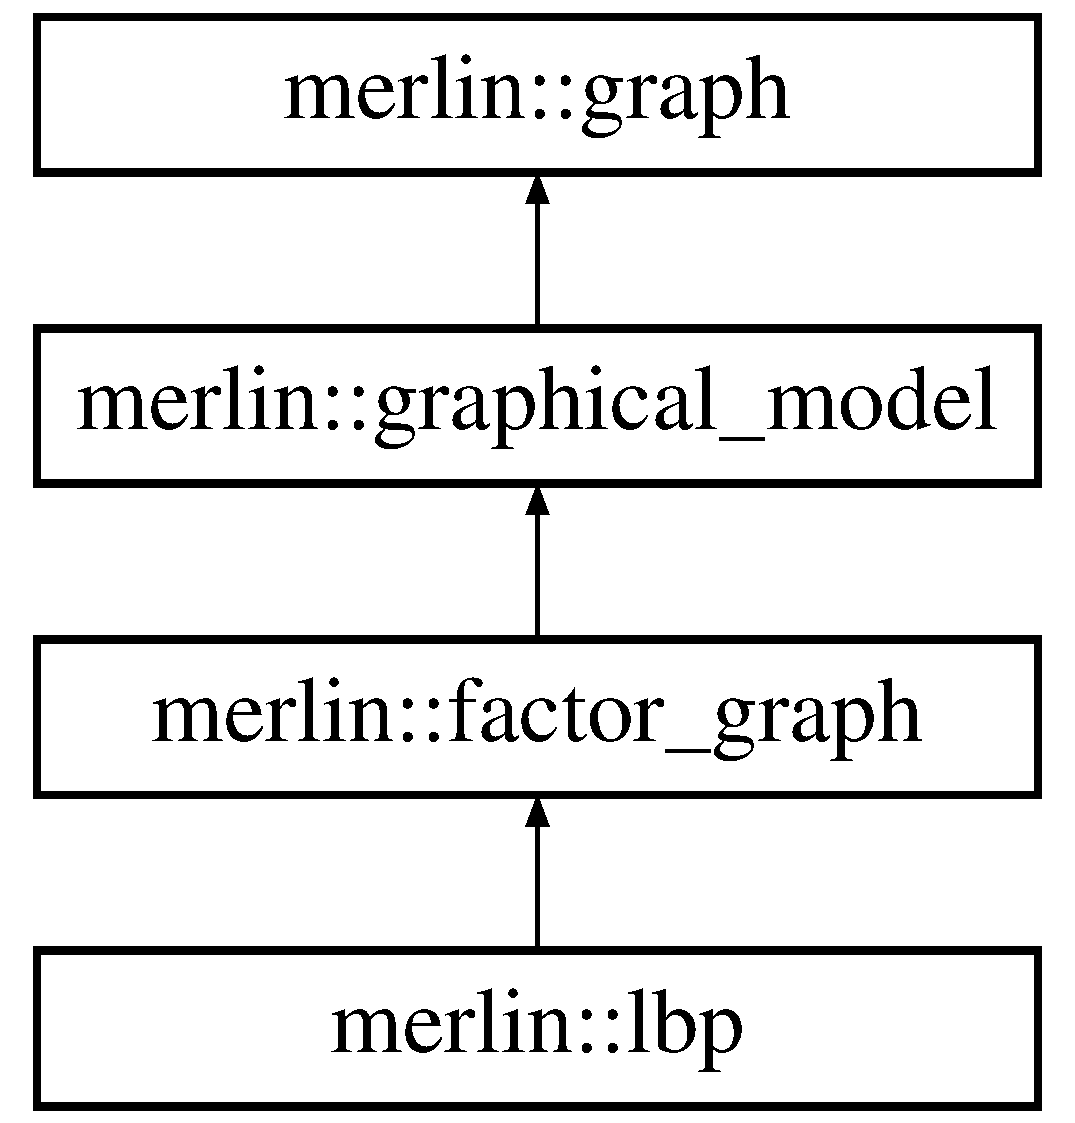
\includegraphics[height=4.000000cm]{classmerlin_1_1factor__graph}
\end{center}
\end{figure}
\subsection*{Classes}
\begin{DoxyCompactItemize}
\item 
class \hyperlink{classmerlin_1_1factor__graph_1_1abstract__queue}{abstract\+\_\+queue}
\begin{DoxyCompactList}\small\item\em Queue type wrapper. \end{DoxyCompactList}\item 
class \hyperlink{classmerlin_1_1factor__graph_1_1abstract__queue__fifo}{abstract\+\_\+queue\+\_\+fifo}
\begin{DoxyCompactList}\small\item\em Queue type for breadth-\/first search. \end{DoxyCompactList}\item 
class \hyperlink{classmerlin_1_1factor__graph_1_1abstract__queue__lifo}{abstract\+\_\+queue\+\_\+lifo}
\begin{DoxyCompactList}\small\item\em Stack type for depth-\/first search. \end{DoxyCompactList}\end{DoxyCompactItemize}
\subsection*{Public Types}
\begin{DoxyCompactItemize}
\item 
typedef \hyperlink{classmerlin_1_1graphical__model_ab2b46f09d8142bb68f243ecadbdabb6b}{graphical\+\_\+model\+::findex} \hyperlink{classmerlin_1_1factor__graph_a533556bd4ec6961b63a91a80a8a37508}{findex}\hypertarget{classmerlin_1_1factor__graph_a533556bd4ec6961b63a91a80a8a37508}{}\label{classmerlin_1_1factor__graph_a533556bd4ec6961b63a91a80a8a37508}

\begin{DoxyCompactList}\small\item\em Factor index. \end{DoxyCompactList}\item 
typedef \hyperlink{classmerlin_1_1graphical__model_a275006a490bc09239c12a4d93d53b135}{graphical\+\_\+model\+::vindex} \hyperlink{classmerlin_1_1factor__graph_a6b8a8220d86d6a6f91a8d2c7dd00ddc9}{vindex}\hypertarget{classmerlin_1_1factor__graph_a6b8a8220d86d6a6f91a8d2c7dd00ddc9}{}\label{classmerlin_1_1factor__graph_a6b8a8220d86d6a6f91a8d2c7dd00ddc9}

\begin{DoxyCompactList}\small\item\em Variable index. \end{DoxyCompactList}\item 
typedef \hyperlink{classmerlin_1_1graphical__model_a615e25ec6594615fddfd4c3c4776b99f}{graphical\+\_\+model\+::flist} \hyperlink{classmerlin_1_1factor__graph_a48dec4ea8a655315053984a81fe93ebc}{flist}\hypertarget{classmerlin_1_1factor__graph_a48dec4ea8a655315053984a81fe93ebc}{}\label{classmerlin_1_1factor__graph_a48dec4ea8a655315053984a81fe93ebc}

\begin{DoxyCompactList}\small\item\em Collection of factor indices. \end{DoxyCompactList}\end{DoxyCompactItemize}
\subsection*{Public Member Functions}
\begin{DoxyCompactItemize}
\item 
\hyperlink{classmerlin_1_1factor__graph_a6a662ba842145071605d68e998e45a98}{factor\+\_\+graph} ()\hypertarget{classmerlin_1_1factor__graph_a6a662ba842145071605d68e998e45a98}{}\label{classmerlin_1_1factor__graph_a6a662ba842145071605d68e998e45a98}

\begin{DoxyCompactList}\small\item\em Default constructor. \end{DoxyCompactList}\item 
\hyperlink{classmerlin_1_1factor__graph_ad7a6caf6041a1911e3afa977c4c9f06c}{factor\+\_\+graph} (const \hyperlink{classmerlin_1_1factor__graph}{factor\+\_\+graph} \&fg)
\begin{DoxyCompactList}\small\item\em Copy constructor. \end{DoxyCompactList}\item 
\hyperlink{classmerlin_1_1factor__graph_a6e9a2dd59408c358b2fac0b0d3838c0e}{factor\+\_\+graph} (std\+::vector$<$ \hyperlink{classmerlin_1_1factor}{factor} $>$ fs)
\begin{DoxyCompactList}\small\item\em Constructor. \end{DoxyCompactList}\item 
{\footnotesize template$<$class Input\+Iterator $>$ }\\\hyperlink{classmerlin_1_1factor__graph_a9f5604018fec35a52f098203833f7618}{factor\+\_\+graph} (Input\+Iterator first, Input\+Iterator last)
\begin{DoxyCompactList}\small\item\em Constructor. \end{DoxyCompactList}\item 
virtual \hyperlink{classmerlin_1_1factor__graph}{factor\+\_\+graph} $\ast$ \hyperlink{classmerlin_1_1factor__graph_a485d9039df843d2db668782ac9c90c8a}{clone} ()
\begin{DoxyCompactList}\small\item\em Clone the factor graph. \end{DoxyCompactList}\item 
\hyperlink{classmerlin_1_1factor__graph_a533556bd4ec6961b63a91a80a8a37508}{findex} \hyperlink{classmerlin_1_1factor__graph_a5899fc5d235ad8681c1437e2845f798d}{add\+\_\+factor} (const \hyperlink{classmerlin_1_1factor}{factor} \&F)
\begin{DoxyCompactList}\small\item\em Add a new factor to the graphical model. \end{DoxyCompactList}\item 
void \hyperlink{classmerlin_1_1factor__graph_aa7a98b7b90992b7dcab7a7b35793fc1f}{remove\+\_\+factor} (\hyperlink{classmerlin_1_1factor__graph_a533556bd4ec6961b63a91a80a8a37508}{findex} f)
\begin{DoxyCompactList}\small\item\em Remove a factor from the model. \end{DoxyCompactList}\item 
\hyperlink{classmerlin_1_1factor__graph_a533556bd4ec6961b63a91a80a8a37508}{findex} \hyperlink{classmerlin_1_1factor__graph_ae1afcb1e51c9a18d15c5cadc37a4ca8b}{local\+\_\+factor} (\hyperlink{classmerlin_1_1factor__graph_a6b8a8220d86d6a6f91a8d2c7dd00ddc9}{vindex} i) const 
\begin{DoxyCompactList}\small\item\em Retrieve the factor index corresponding to a variable node. \end{DoxyCompactList}\item 
\hyperlink{classmerlin_1_1factor__graph_a533556bd4ec6961b63a91a80a8a37508}{findex} \hyperlink{classmerlin_1_1factor__graph_ad4789b9f75a841d7170c6bc4e8912b26}{local\+\_\+factor} (\hyperlink{classmerlin_1_1variable}{variable} v) const 
\begin{DoxyCompactList}\small\item\em Retrieve the factor index corresponding to a variable node. \end{DoxyCompactList}\item 
bool \hyperlink{classmerlin_1_1factor__graph_ac0632388a94e4ed45ed31a5130043f14}{is\+\_\+var\+\_\+node} (\hyperlink{classmerlin_1_1factor__graph_a533556bd4ec6961b63a91a80a8a37508}{findex} i) const 
\begin{DoxyCompactList}\small\item\em Check if a factor is a variable node in the factor graph. \end{DoxyCompactList}\item 
\hyperlink{classmerlin_1_1factor__graph_a48dec4ea8a655315053984a81fe93ebc}{flist} \hyperlink{classmerlin_1_1factor__graph_a88b2d9a79901b3dbfda925f61fa070e2}{adjacent\+\_\+factors} (\hyperlink{classmerlin_1_1variable}{variable} v) const 
\begin{DoxyCompactList}\small\item\em Retrieve the factors adjacent to a variable node in the factor graph. \end{DoxyCompactList}\item 
\hyperlink{classmerlin_1_1factor__graph_a48dec4ea8a655315053984a81fe93ebc}{flist} \hyperlink{classmerlin_1_1factor__graph_acad131cfcb6750093683128ab7171523}{adjacent\+\_\+factors} (\hyperlink{classmerlin_1_1factor__graph_a6b8a8220d86d6a6f91a8d2c7dd00ddc9}{vindex} v) const 
\begin{DoxyCompactList}\small\item\em Retrieve the factors adjacent to a variable node in the factor graph. \end{DoxyCompactList}\item 
\hyperlink{classmerlin_1_1variable__set}{variable\+\_\+set} \hyperlink{classmerlin_1_1factor__graph_a84f3800e16143f385dd14afedd7d49ef}{adjacent\+\_\+vars} (\hyperlink{classmerlin_1_1factor__graph_a533556bd4ec6961b63a91a80a8a37508}{findex} f) const 
\begin{DoxyCompactList}\small\item\em Retrieve the variables adjacent to a factor in the factor graph. \end{DoxyCompactList}\item 
void \hyperlink{classmerlin_1_1factor__graph_a5cdf18711449fed75507d80bbfe549fb}{swap} (\hyperlink{classmerlin_1_1factor__graph}{factor\+\_\+graph} \&gm)
\begin{DoxyCompactList}\small\item\em Swap the contents of two factor graphs. \end{DoxyCompactList}\item 
\hyperlink{classmerlin_1_1factor__graph_ae9d805687c0de6a98a423b12987d0847}{M\+E\+R\+\_\+\+E\+N\+UM} (Tree\+Type, Width\+First, Depth\+First, Max\+Weight)\hypertarget{classmerlin_1_1factor__graph_ae9d805687c0de6a98a423b12987d0847}{}\label{classmerlin_1_1factor__graph_ae9d805687c0de6a98a423b12987d0847}

\begin{DoxyCompactList}\small\item\em Type of tree. \end{DoxyCompactList}\item 
std\+::vector$<$ \hyperlink{namespacemerlin_a44eb24328668c9618f20915763bd3192}{edge\+\_\+t} $>$ \hyperlink{classmerlin_1_1factor__graph_a15aa43072a0d40884957b7053106d5fb}{span\+\_\+tree} (Tree\+Type tt, \hyperlink{classmerlin_1_1variable}{variable} root)
\begin{DoxyCompactList}\small\item\em Create a spanning tree of the factor graph. \end{DoxyCompactList}\item 
std\+::vector$<$ \hyperlink{namespacemerlin_a44eb24328668c9618f20915763bd3192}{edge\+\_\+t} $>$ \hyperlink{classmerlin_1_1factor__graph_add951d3edd3613808615b87fa2201904}{span\+\_\+tree} (Tree\+Type tt=Tree\+Type\+::\+Width\+First)
\begin{DoxyCompactList}\small\item\em Create a spanning tree of the factor graph rooted by a randomly selected variable. \end{DoxyCompactList}\end{DoxyCompactItemize}
\subsection*{Protected Types}
\begin{DoxyCompactItemize}
\item 
typedef size\+\_\+t \hyperlink{classmerlin_1_1factor__graph_abec36f1f1a6ff2c0bfb74299851f9722}{eindex}\hypertarget{classmerlin_1_1factor__graph_abec36f1f1a6ff2c0bfb74299851f9722}{}\label{classmerlin_1_1factor__graph_abec36f1f1a6ff2c0bfb74299851f9722}

\begin{DoxyCompactList}\small\item\em Edge index. \end{DoxyCompactList}\end{DoxyCompactItemize}
\subsection*{Protected Member Functions}
\begin{DoxyCompactItemize}
\item 
\hyperlink{classmerlin_1_1factor__graph_a48dec4ea8a655315053984a81fe93ebc}{flist} \hyperlink{classmerlin_1_1factor__graph_a54f75765bae775dfa08f0ba4b022ea87}{\+\_\+neighbors} (\hyperlink{classmerlin_1_1factor__graph_a533556bd4ec6961b63a91a80a8a37508}{findex} i) const 
\begin{DoxyCompactList}\small\item\em Retrieve the neighbors of a factor. \end{DoxyCompactList}\item 
void \hyperlink{classmerlin_1_1factor__graph_ab9e0014c667318cdfe9454dc6bb3bf8a}{create\+\_\+factor\+\_\+graph} ()
\begin{DoxyCompactList}\small\item\em Create the factor graph. \end{DoxyCompactList}\item 
\hyperlink{classmerlin_1_1factor__graph_abec36f1f1a6ff2c0bfb74299851f9722}{eindex} \hyperlink{classmerlin_1_1factor__graph_ad167336dbf3fa30cfb4844c3d4fd1a37}{\+\_\+eindex} (\hyperlink{classmerlin_1_1factor__graph_a533556bd4ec6961b63a91a80a8a37508}{findex} i, \hyperlink{classmerlin_1_1factor__graph_a533556bd4ec6961b63a91a80a8a37508}{findex} j)
\begin{DoxyCompactList}\small\item\em Retrieve the index of the edge between two nodes. \end{DoxyCompactList}\end{DoxyCompactItemize}
\subsection*{Protected Attributes}
\begin{DoxyCompactItemize}
\item 
std\+::vector$<$ size\+\_\+t $>$ \hyperlink{classmerlin_1_1factor__graph_a0bbad915cf9b946de03f94670616cf80}{m\+\_\+vindex}\hypertarget{classmerlin_1_1factor__graph_a0bbad915cf9b946de03f94670616cf80}{}\label{classmerlin_1_1factor__graph_a0bbad915cf9b946de03f94670616cf80}

\begin{DoxyCompactList}\small\item\em Factors representing variable nodes in factor graph. \end{DoxyCompactList}\end{DoxyCompactItemize}
\subsection*{Additional Inherited Members}


\subsection{Detailed Description}
A factor graph base class. 

A graphical model represented as a bipartite graph between {\itshape variable nodes}, corresponding to the variables, and {\itshape factor nodes}, corresponding to the factors. Internally, factors and variables are mainly referenced by integer indices, with 0 $<$= f $<$ n\+Factors() and 0 $<$= v $<$ \hyperlink{classmerlin_1_1graphical__model_af70ee4f7a4414fac4f7568e3c0e5efca}{nvar()}. However, many interface functions are called using a variable object, var(label,dim). To convert, var(v) gives the vth var object and the internal function \+\_\+vindex(\+V) gives the index corresponding to variable object V. 

Definition at line 44 of file factor\+\_\+graph.\+h.



\subsection{Constructor \& Destructor Documentation}
\index{merlin\+::factor\+\_\+graph@{merlin\+::factor\+\_\+graph}!factor\+\_\+graph@{factor\+\_\+graph}}
\index{factor\+\_\+graph@{factor\+\_\+graph}!merlin\+::factor\+\_\+graph@{merlin\+::factor\+\_\+graph}}
\subsubsection[{\texorpdfstring{factor\+\_\+graph(const factor\+\_\+graph \&fg)}{factor_graph(const factor_graph &fg)}}]{\setlength{\rightskip}{0pt plus 5cm}merlin\+::factor\+\_\+graph\+::factor\+\_\+graph (
\begin{DoxyParamCaption}
\item[{const {\bf factor\+\_\+graph} \&}]{fg}
\end{DoxyParamCaption}
)\hspace{0.3cm}{\ttfamily [inline]}}\hypertarget{classmerlin_1_1factor__graph_ad7a6caf6041a1911e3afa977c4c9f06c}{}\label{classmerlin_1_1factor__graph_ad7a6caf6041a1911e3afa977c4c9f06c}


Copy constructor. 


\begin{DoxyParams}{Parameters}
{\em fg} & The factor graph to be copied \\
\hline
\end{DoxyParams}


Definition at line 66 of file factor\+\_\+graph.\+h.

\index{merlin\+::factor\+\_\+graph@{merlin\+::factor\+\_\+graph}!factor\+\_\+graph@{factor\+\_\+graph}}
\index{factor\+\_\+graph@{factor\+\_\+graph}!merlin\+::factor\+\_\+graph@{merlin\+::factor\+\_\+graph}}
\subsubsection[{\texorpdfstring{factor\+\_\+graph(std\+::vector$<$ factor $>$ fs)}{factor_graph(std::vector< factor > fs)}}]{\setlength{\rightskip}{0pt plus 5cm}merlin\+::factor\+\_\+graph\+::factor\+\_\+graph (
\begin{DoxyParamCaption}
\item[{std\+::vector$<$ {\bf factor} $>$}]{fs}
\end{DoxyParamCaption}
)\hspace{0.3cm}{\ttfamily [inline]}}\hypertarget{classmerlin_1_1factor__graph_a6e9a2dd59408c358b2fac0b0d3838c0e}{}\label{classmerlin_1_1factor__graph_a6e9a2dd59408c358b2fac0b0d3838c0e}


Constructor. 


\begin{DoxyParams}{Parameters}
{\em fs} & The list of factors \\
\hline
\end{DoxyParams}


Definition at line 74 of file factor\+\_\+graph.\+h.



References create\+\_\+factor\+\_\+graph(), m\+\_\+vindex, and merlin\+::graphical\+\_\+model\+::nvar().

\index{merlin\+::factor\+\_\+graph@{merlin\+::factor\+\_\+graph}!factor\+\_\+graph@{factor\+\_\+graph}}
\index{factor\+\_\+graph@{factor\+\_\+graph}!merlin\+::factor\+\_\+graph@{merlin\+::factor\+\_\+graph}}
\subsubsection[{\texorpdfstring{factor\+\_\+graph(\+Input\+Iterator first, Input\+Iterator last)}{factor_graph(InputIterator first, InputIterator last)}}]{\setlength{\rightskip}{0pt plus 5cm}template$<$class Input\+Iterator $>$ merlin\+::factor\+\_\+graph\+::factor\+\_\+graph (
\begin{DoxyParamCaption}
\item[{Input\+Iterator}]{first, }
\item[{Input\+Iterator}]{last}
\end{DoxyParamCaption}
)\hspace{0.3cm}{\ttfamily [inline]}}\hypertarget{classmerlin_1_1factor__graph_a9f5604018fec35a52f098203833f7618}{}\label{classmerlin_1_1factor__graph_a9f5604018fec35a52f098203833f7618}


Constructor. 


\begin{DoxyParams}{Parameters}
{\em first} & The {\itshape begin} iterator of the factors list \\
\hline
{\em last} & The {\itshape end} iterator of the factors list \\
\hline
\end{DoxyParams}


Definition at line 85 of file factor\+\_\+graph.\+h.



References create\+\_\+factor\+\_\+graph(), m\+\_\+vindex, and merlin\+::graphical\+\_\+model\+::nvar().



\subsection{Member Function Documentation}
\index{merlin\+::factor\+\_\+graph@{merlin\+::factor\+\_\+graph}!\+\_\+eindex@{\+\_\+eindex}}
\index{\+\_\+eindex@{\+\_\+eindex}!merlin\+::factor\+\_\+graph@{merlin\+::factor\+\_\+graph}}
\subsubsection[{\texorpdfstring{\+\_\+eindex(findex i, findex j)}{_eindex(findex i, findex j)}}]{\setlength{\rightskip}{0pt plus 5cm}{\bf eindex} merlin\+::factor\+\_\+graph\+::\+\_\+eindex (
\begin{DoxyParamCaption}
\item[{{\bf findex}}]{i, }
\item[{{\bf findex}}]{j}
\end{DoxyParamCaption}
)\hspace{0.3cm}{\ttfamily [inline]}, {\ttfamily [protected]}}\hypertarget{classmerlin_1_1factor__graph_ad167336dbf3fa30cfb4844c3d4fd1a37}{}\label{classmerlin_1_1factor__graph_ad167336dbf3fa30cfb4844c3d4fd1a37}


Retrieve the index of the edge between two nodes. 


\begin{DoxyParams}{Parameters}
{\em i} & The (factor) index of the head \\
\hline
{\em j} & The (factor) index of the tail \\
\hline
\end{DoxyParams}
\begin{DoxyReturn}{Returns}
the index of the edge between the two factors. 
\end{DoxyReturn}


Definition at line 269 of file factor\+\_\+graph.\+h.



References merlin\+::graph\+::edge(), and merlin\+::edge\+\_\+id\+::idx.

\index{merlin\+::factor\+\_\+graph@{merlin\+::factor\+\_\+graph}!\+\_\+neighbors@{\+\_\+neighbors}}
\index{\+\_\+neighbors@{\+\_\+neighbors}!merlin\+::factor\+\_\+graph@{merlin\+::factor\+\_\+graph}}
\subsubsection[{\texorpdfstring{\+\_\+neighbors(findex i) const }{_neighbors(findex i) const }}]{\setlength{\rightskip}{0pt plus 5cm}{\bf flist} merlin\+::factor\+\_\+graph\+::\+\_\+neighbors (
\begin{DoxyParamCaption}
\item[{{\bf findex}}]{i}
\end{DoxyParamCaption}
) const\hspace{0.3cm}{\ttfamily [inline]}, {\ttfamily [protected]}}\hypertarget{classmerlin_1_1factor__graph_a54f75765bae775dfa08f0ba4b022ea87}{}\label{classmerlin_1_1factor__graph_a54f75765bae775dfa08f0ba4b022ea87}


Retrieve the neighbors of a factor. 


\begin{DoxyParams}{Parameters}
{\em i} & The index of the factor \\
\hline
\end{DoxyParams}
\begin{DoxyReturn}{Returns}
the list of factor indexes that are connected to the input factor. 
\end{DoxyReturn}


Definition at line 207 of file factor\+\_\+graph.\+h.



References merlin\+::graph\+::neighbors().



Referenced by adjacent\+\_\+factors().

\index{merlin\+::factor\+\_\+graph@{merlin\+::factor\+\_\+graph}!add\+\_\+factor@{add\+\_\+factor}}
\index{add\+\_\+factor@{add\+\_\+factor}!merlin\+::factor\+\_\+graph@{merlin\+::factor\+\_\+graph}}
\subsubsection[{\texorpdfstring{add\+\_\+factor(const factor \&\+F)}{add_factor(const factor &F)}}]{\setlength{\rightskip}{0pt plus 5cm}{\bf findex} merlin\+::factor\+\_\+graph\+::add\+\_\+factor (
\begin{DoxyParamCaption}
\item[{const {\bf factor} \&}]{F}
\end{DoxyParamCaption}
)\hspace{0.3cm}{\ttfamily [inline]}, {\ttfamily [virtual]}}\hypertarget{classmerlin_1_1factor__graph_a5899fc5d235ad8681c1437e2845f798d}{}\label{classmerlin_1_1factor__graph_a5899fc5d235ad8681c1437e2845f798d}


Add a new factor to the graphical model. 


\begin{DoxyParams}{Parameters}
{\em F} & The factor to be added \\
\hline
\end{DoxyParams}
\begin{DoxyReturn}{Returns}
the index of the newly added factor. 
\end{DoxyReturn}


Reimplemented from \hyperlink{classmerlin_1_1graphical__model_a7edaca0ce3ddea09f64e6bab406bfab8}{merlin\+::graphical\+\_\+model}.



Definition at line 105 of file factor\+\_\+graph.\+h.



References merlin\+::graph\+::add\+\_\+edge(), merlin\+::graphical\+\_\+model\+::add\+\_\+factor(), merlin\+::variable\+\_\+set\+::begin(), merlin\+::variable\+\_\+set\+::end(), local\+\_\+factor(), m\+\_\+vindex, merlin\+::factor\+::nvar(), merlin\+::graphical\+\_\+model\+::nvar(), and merlin\+::factor\+::vars().

\index{merlin\+::factor\+\_\+graph@{merlin\+::factor\+\_\+graph}!adjacent\+\_\+factors@{adjacent\+\_\+factors}}
\index{adjacent\+\_\+factors@{adjacent\+\_\+factors}!merlin\+::factor\+\_\+graph@{merlin\+::factor\+\_\+graph}}
\subsubsection[{\texorpdfstring{adjacent\+\_\+factors(variable v) const }{adjacent_factors(variable v) const }}]{\setlength{\rightskip}{0pt plus 5cm}{\bf flist} merlin\+::factor\+\_\+graph\+::adjacent\+\_\+factors (
\begin{DoxyParamCaption}
\item[{{\bf variable}}]{v}
\end{DoxyParamCaption}
) const\hspace{0.3cm}{\ttfamily [inline]}}\hypertarget{classmerlin_1_1factor__graph_a88b2d9a79901b3dbfda925f61fa070e2}{}\label{classmerlin_1_1factor__graph_a88b2d9a79901b3dbfda925f61fa070e2}


Retrieve the factors adjacent to a variable node in the factor graph. 


\begin{DoxyParams}{Parameters}
{\em v} & The index of the variable \\
\hline
\end{DoxyParams}
\begin{DoxyReturn}{Returns}
the list of factor indexes corresponding to the adjacent factors. 
\end{DoxyReturn}


Definition at line 170 of file factor\+\_\+graph.\+h.



References \+\_\+neighbors(), and local\+\_\+factor().

\index{merlin\+::factor\+\_\+graph@{merlin\+::factor\+\_\+graph}!adjacent\+\_\+factors@{adjacent\+\_\+factors}}
\index{adjacent\+\_\+factors@{adjacent\+\_\+factors}!merlin\+::factor\+\_\+graph@{merlin\+::factor\+\_\+graph}}
\subsubsection[{\texorpdfstring{adjacent\+\_\+factors(vindex v) const }{adjacent_factors(vindex v) const }}]{\setlength{\rightskip}{0pt plus 5cm}{\bf flist} merlin\+::factor\+\_\+graph\+::adjacent\+\_\+factors (
\begin{DoxyParamCaption}
\item[{{\bf vindex}}]{v}
\end{DoxyParamCaption}
) const\hspace{0.3cm}{\ttfamily [inline]}}\hypertarget{classmerlin_1_1factor__graph_acad131cfcb6750093683128ab7171523}{}\label{classmerlin_1_1factor__graph_acad131cfcb6750093683128ab7171523}


Retrieve the factors adjacent to a variable node in the factor graph. 


\begin{DoxyParams}{Parameters}
{\em v} & The index of the variable \\
\hline
\end{DoxyParams}
\begin{DoxyReturn}{Returns}
the list of factor indexes corresponding to the adjacent factors. 
\end{DoxyReturn}


Definition at line 179 of file factor\+\_\+graph.\+h.



References \+\_\+neighbors(), and local\+\_\+factor().

\index{merlin\+::factor\+\_\+graph@{merlin\+::factor\+\_\+graph}!adjacent\+\_\+vars@{adjacent\+\_\+vars}}
\index{adjacent\+\_\+vars@{adjacent\+\_\+vars}!merlin\+::factor\+\_\+graph@{merlin\+::factor\+\_\+graph}}
\subsubsection[{\texorpdfstring{adjacent\+\_\+vars(findex f) const }{adjacent_vars(findex f) const }}]{\setlength{\rightskip}{0pt plus 5cm}{\bf variable\+\_\+set} merlin\+::factor\+\_\+graph\+::adjacent\+\_\+vars (
\begin{DoxyParamCaption}
\item[{{\bf findex}}]{f}
\end{DoxyParamCaption}
) const\hspace{0.3cm}{\ttfamily [inline]}}\hypertarget{classmerlin_1_1factor__graph_a84f3800e16143f385dd14afedd7d49ef}{}\label{classmerlin_1_1factor__graph_a84f3800e16143f385dd14afedd7d49ef}


Retrieve the variables adjacent to a factor in the factor graph. 


\begin{DoxyParams}{Parameters}
{\em f} & The index of the factor \\
\hline
\end{DoxyParams}
\begin{DoxyReturn}{Returns}
the list of variable indexes corresponding to the adjacent variables. 
\end{DoxyReturn}


Definition at line 188 of file factor\+\_\+graph.\+h.



References merlin\+::graphical\+\_\+model\+::get\+\_\+factor(), swap(), and merlin\+::factor\+::vars().



Referenced by merlin\+::lbp\+::obj\+\_\+entropy().

\index{merlin\+::factor\+\_\+graph@{merlin\+::factor\+\_\+graph}!clone@{clone}}
\index{clone@{clone}!merlin\+::factor\+\_\+graph@{merlin\+::factor\+\_\+graph}}
\subsubsection[{\texorpdfstring{clone()}{clone()}}]{\setlength{\rightskip}{0pt plus 5cm}virtual {\bf factor\+\_\+graph}$\ast$ merlin\+::factor\+\_\+graph\+::clone (
\begin{DoxyParamCaption}
{}
\end{DoxyParamCaption}
)\hspace{0.3cm}{\ttfamily [inline]}, {\ttfamily [virtual]}}\hypertarget{classmerlin_1_1factor__graph_a485d9039df843d2db668782ac9c90c8a}{}\label{classmerlin_1_1factor__graph_a485d9039df843d2db668782ac9c90c8a}


Clone the factor graph. 

\begin{DoxyReturn}{Returns}
a pointer to the cloned factor graph. 
\end{DoxyReturn}


Reimplemented from \hyperlink{classmerlin_1_1graphical__model_a5315423e0cda62c03beda959b1311f48}{merlin\+::graphical\+\_\+model}.



Definition at line 95 of file factor\+\_\+graph.\+h.



References factor\+\_\+graph().

\index{merlin\+::factor\+\_\+graph@{merlin\+::factor\+\_\+graph}!create\+\_\+factor\+\_\+graph@{create\+\_\+factor\+\_\+graph}}
\index{create\+\_\+factor\+\_\+graph@{create\+\_\+factor\+\_\+graph}!merlin\+::factor\+\_\+graph@{merlin\+::factor\+\_\+graph}}
\subsubsection[{\texorpdfstring{create\+\_\+factor\+\_\+graph()}{create_factor_graph()}}]{\setlength{\rightskip}{0pt plus 5cm}void merlin\+::factor\+\_\+graph\+::create\+\_\+factor\+\_\+graph (
\begin{DoxyParamCaption}
{}
\end{DoxyParamCaption}
)\hspace{0.3cm}{\ttfamily [inline]}, {\ttfamily [protected]}}\hypertarget{classmerlin_1_1factor__graph_ab9e0014c667318cdfe9454dc6bb3bf8a}{}\label{classmerlin_1_1factor__graph_ab9e0014c667318cdfe9454dc6bb3bf8a}


Create the factor graph. 

Creates the bi-\/partite graph by adding nodes corresponding to local variable factors (ie, unary factors definded for each variable) and connecting them to the nodes corresponding to the factors. Let M be the number of factors. Then the nodes corresponding to the factors are indexed \mbox{[}0 .. M-\/1\mbox{]}, while the nodes corresponding to the variables are indexed \mbox{[}M .. M+\+N-\/1\mbox{]} where N is the number of variables. 

Definition at line 226 of file factor\+\_\+graph.\+h.



References merlin\+::graphical\+\_\+model\+::\+\_\+vindex(), merlin\+::graph\+::add\+\_\+edge(), merlin\+::graphical\+\_\+model\+::add\+\_\+factor(), is\+\_\+var\+\_\+node(), local\+\_\+factor(), merlin\+::graphical\+\_\+model\+::m\+\_\+factors, m\+\_\+vindex, merlin\+::graph\+::num\+\_\+edges(), merlin\+::graphical\+\_\+model\+::nvar(), and merlin\+::graphical\+\_\+model\+::var().



Referenced by factor\+\_\+graph().

\index{merlin\+::factor\+\_\+graph@{merlin\+::factor\+\_\+graph}!is\+\_\+var\+\_\+node@{is\+\_\+var\+\_\+node}}
\index{is\+\_\+var\+\_\+node@{is\+\_\+var\+\_\+node}!merlin\+::factor\+\_\+graph@{merlin\+::factor\+\_\+graph}}
\subsubsection[{\texorpdfstring{is\+\_\+var\+\_\+node(findex i) const }{is_var_node(findex i) const }}]{\setlength{\rightskip}{0pt plus 5cm}bool merlin\+::factor\+\_\+graph\+::is\+\_\+var\+\_\+node (
\begin{DoxyParamCaption}
\item[{{\bf findex}}]{i}
\end{DoxyParamCaption}
) const\hspace{0.3cm}{\ttfamily [inline]}}\hypertarget{classmerlin_1_1factor__graph_ac0632388a94e4ed45ed31a5130043f14}{}\label{classmerlin_1_1factor__graph_ac0632388a94e4ed45ed31a5130043f14}


Check if a factor is a variable node in the factor graph. 


\begin{DoxyParams}{Parameters}
{\em i} & The index of the factor \\
\hline
\end{DoxyParams}
\begin{DoxyReturn}{Returns}
{\itshape true} if the factor corresponds to a variable node, and {\itshape false} otherwise. 
\end{DoxyReturn}


Definition at line 160 of file factor\+\_\+graph.\+h.



References merlin\+::graphical\+\_\+model\+::get\+\_\+factor(), local\+\_\+factor(), and merlin\+::graphical\+\_\+model\+::nvar().



Referenced by create\+\_\+factor\+\_\+graph(), merlin\+::lbp\+::init(), merlin\+::lbp\+::obj\+\_\+entropy(), and span\+\_\+tree().

\index{merlin\+::factor\+\_\+graph@{merlin\+::factor\+\_\+graph}!local\+\_\+factor@{local\+\_\+factor}}
\index{local\+\_\+factor@{local\+\_\+factor}!merlin\+::factor\+\_\+graph@{merlin\+::factor\+\_\+graph}}
\subsubsection[{\texorpdfstring{local\+\_\+factor(vindex i) const }{local_factor(vindex i) const }}]{\setlength{\rightskip}{0pt plus 5cm}{\bf findex} merlin\+::factor\+\_\+graph\+::local\+\_\+factor (
\begin{DoxyParamCaption}
\item[{{\bf vindex}}]{i}
\end{DoxyParamCaption}
) const\hspace{0.3cm}{\ttfamily [inline]}}\hypertarget{classmerlin_1_1factor__graph_ae1afcb1e51c9a18d15c5cadc37a4ca8b}{}\label{classmerlin_1_1factor__graph_ae1afcb1e51c9a18d15c5cadc37a4ca8b}


Retrieve the factor index corresponding to a variable node. 


\begin{DoxyParams}{Parameters}
{\em i} & The index of a variable \\
\hline
\end{DoxyParams}
\begin{DoxyReturn}{Returns}
the index of the factor associated with the variable in the factor graph. 
\end{DoxyReturn}


Definition at line 140 of file factor\+\_\+graph.\+h.



References m\+\_\+vindex.



Referenced by add\+\_\+factor(), adjacent\+\_\+factors(), merlin\+::lbp\+::belief(), create\+\_\+factor\+\_\+graph(), is\+\_\+var\+\_\+node(), remove\+\_\+factor(), and span\+\_\+tree().

\index{merlin\+::factor\+\_\+graph@{merlin\+::factor\+\_\+graph}!local\+\_\+factor@{local\+\_\+factor}}
\index{local\+\_\+factor@{local\+\_\+factor}!merlin\+::factor\+\_\+graph@{merlin\+::factor\+\_\+graph}}
\subsubsection[{\texorpdfstring{local\+\_\+factor(variable v) const }{local_factor(variable v) const }}]{\setlength{\rightskip}{0pt plus 5cm}{\bf findex} merlin\+::factor\+\_\+graph\+::local\+\_\+factor (
\begin{DoxyParamCaption}
\item[{{\bf variable}}]{v}
\end{DoxyParamCaption}
) const\hspace{0.3cm}{\ttfamily [inline]}}\hypertarget{classmerlin_1_1factor__graph_ad4789b9f75a841d7170c6bc4e8912b26}{}\label{classmerlin_1_1factor__graph_ad4789b9f75a841d7170c6bc4e8912b26}


Retrieve the factor index corresponding to a variable node. 


\begin{DoxyParams}{Parameters}
{\em v} & The index of a variable \\
\hline
\end{DoxyParams}
\begin{DoxyReturn}{Returns}
the index of the factor associated with the variable in the factor graph. 
\end{DoxyReturn}


Definition at line 150 of file factor\+\_\+graph.\+h.



References merlin\+::graphical\+\_\+model\+::\+\_\+vindex(), and m\+\_\+vindex.

\index{merlin\+::factor\+\_\+graph@{merlin\+::factor\+\_\+graph}!remove\+\_\+factor@{remove\+\_\+factor}}
\index{remove\+\_\+factor@{remove\+\_\+factor}!merlin\+::factor\+\_\+graph@{merlin\+::factor\+\_\+graph}}
\subsubsection[{\texorpdfstring{remove\+\_\+factor(findex f)}{remove_factor(findex f)}}]{\setlength{\rightskip}{0pt plus 5cm}void merlin\+::factor\+\_\+graph\+::remove\+\_\+factor (
\begin{DoxyParamCaption}
\item[{{\bf findex}}]{f}
\end{DoxyParamCaption}
)\hspace{0.3cm}{\ttfamily [inline]}, {\ttfamily [virtual]}}\hypertarget{classmerlin_1_1factor__graph_aa7a98b7b90992b7dcab7a7b35793fc1f}{}\label{classmerlin_1_1factor__graph_aa7a98b7b90992b7dcab7a7b35793fc1f}


Remove a factor from the model. 


\begin{DoxyParams}{Parameters}
{\em f} & The index of the factor to be removed \\
\hline
\end{DoxyParams}


Reimplemented from \hyperlink{classmerlin_1_1graphical__model_aabcdb025068a429bc1ab8d62e38065d9}{merlin\+::graphical\+\_\+model}.



Definition at line 124 of file factor\+\_\+graph.\+h.



References merlin\+::graphical\+\_\+model\+::\+\_\+vindex(), merlin\+::variable\+\_\+set\+::begin(), merlin\+::variable\+\_\+set\+::end(), local\+\_\+factor(), merlin\+::graphical\+\_\+model\+::m\+\_\+factors, m\+\_\+vindex, merlin\+::graph\+::remove\+\_\+edge(), and merlin\+::graphical\+\_\+model\+::remove\+\_\+factor().

\index{merlin\+::factor\+\_\+graph@{merlin\+::factor\+\_\+graph}!span\+\_\+tree@{span\+\_\+tree}}
\index{span\+\_\+tree@{span\+\_\+tree}!merlin\+::factor\+\_\+graph@{merlin\+::factor\+\_\+graph}}
\subsubsection[{\texorpdfstring{span\+\_\+tree(\+Tree\+Type tt, variable root)}{span_tree(TreeType tt, variable root)}}]{\setlength{\rightskip}{0pt plus 5cm}std\+::vector$<${\bf edge\+\_\+t}$>$ merlin\+::factor\+\_\+graph\+::span\+\_\+tree (
\begin{DoxyParamCaption}
\item[{Tree\+Type}]{tt, }
\item[{{\bf variable}}]{root}
\end{DoxyParamCaption}
)\hspace{0.3cm}{\ttfamily [inline]}}\hypertarget{classmerlin_1_1factor__graph_a15aa43072a0d40884957b7053106d5fb}{}\label{classmerlin_1_1factor__graph_a15aa43072a0d40884957b7053106d5fb}


Create a spanning tree of the factor graph. 


\begin{DoxyParams}{Parameters}
{\em tt} & The type of spanning tree \\
\hline
{\em root} & The root (variable index) of the spanning tree \\
\hline
\end{DoxyParams}
\begin{DoxyReturn}{Returns}
the spanning tree as a list of edge indexes in the factor graph. 
\end{DoxyReturn}


Definition at line 344 of file factor\+\_\+graph.\+h.



References merlin\+::graphical\+\_\+model\+::\+\_\+vindex(), merlin\+::set$<$ T $>$\+::begin(), merlin\+::variable\+\_\+set\+::begin(), merlin\+::set$<$ T $>$\+::end(), merlin\+::variable\+\_\+set\+::end(), merlin\+::graphical\+\_\+model\+::get\+\_\+factor(), is\+\_\+var\+\_\+node(), local\+\_\+factor(), merlin\+::graph\+::neighbors(), merlin\+::graphical\+\_\+model\+::num\+\_\+factors(), merlin\+::graphical\+\_\+model\+::nvar(), and merlin\+::factor\+::vars().



Referenced by span\+\_\+tree().

\index{merlin\+::factor\+\_\+graph@{merlin\+::factor\+\_\+graph}!span\+\_\+tree@{span\+\_\+tree}}
\index{span\+\_\+tree@{span\+\_\+tree}!merlin\+::factor\+\_\+graph@{merlin\+::factor\+\_\+graph}}
\subsubsection[{\texorpdfstring{span\+\_\+tree(\+Tree\+Type tt=\+Tree\+Type\+::\+Width\+First)}{span_tree(TreeType tt=TreeType::WidthFirst)}}]{\setlength{\rightskip}{0pt plus 5cm}std\+::vector$<${\bf edge\+\_\+t}$>$ merlin\+::factor\+\_\+graph\+::span\+\_\+tree (
\begin{DoxyParamCaption}
\item[{Tree\+Type}]{tt = {\ttfamily TreeType\+:\+:WidthFirst}}
\end{DoxyParamCaption}
)\hspace{0.3cm}{\ttfamily [inline]}}\hypertarget{classmerlin_1_1factor__graph_add951d3edd3613808615b87fa2201904}{}\label{classmerlin_1_1factor__graph_add951d3edd3613808615b87fa2201904}


Create a spanning tree of the factor graph rooted by a randomly selected variable. 


\begin{DoxyParams}{Parameters}
{\em tt} & The type of spanning tree \\
\hline
\end{DoxyParams}
\begin{DoxyReturn}{Returns}
the spanning tree as a list of edge indexes in the factor graph. 
\end{DoxyReturn}


Definition at line 408 of file factor\+\_\+graph.\+h.



References merlin\+::graphical\+\_\+model\+::nvar(), span\+\_\+tree(), and merlin\+::graphical\+\_\+model\+::var().

\index{merlin\+::factor\+\_\+graph@{merlin\+::factor\+\_\+graph}!swap@{swap}}
\index{swap@{swap}!merlin\+::factor\+\_\+graph@{merlin\+::factor\+\_\+graph}}
\subsubsection[{\texorpdfstring{swap(factor\+\_\+graph \&gm)}{swap(factor_graph &gm)}}]{\setlength{\rightskip}{0pt plus 5cm}void merlin\+::factor\+\_\+graph\+::swap (
\begin{DoxyParamCaption}
\item[{{\bf factor\+\_\+graph} \&}]{gm}
\end{DoxyParamCaption}
)}\hypertarget{classmerlin_1_1factor__graph_a5cdf18711449fed75507d80bbfe549fb}{}\label{classmerlin_1_1factor__graph_a5cdf18711449fed75507d80bbfe549fb}


Swap the contents of two factor graphs. 


\begin{DoxyParams}{Parameters}
{\em gm} & The factor graph to swap with \\
\hline
\end{DoxyParams}


Referenced by adjacent\+\_\+vars().



The documentation for this class was generated from the following file\+:\begin{DoxyCompactItemize}
\item 
src/include/\hyperlink{factor__graph_8h}{factor\+\_\+graph.\+h}\end{DoxyCompactItemize}

\hypertarget{classmerlin_1_1gibbs}{}\section{merlin\+:\+:gibbs Class Reference}
\label{classmerlin_1_1gibbs}\index{merlin\+::gibbs@{merlin\+::gibbs}}


Factor graph algorithm specialization for Gibbs sampling.  




{\ttfamily \#include $<$gibbs.\+h$>$}

Inheritance diagram for merlin\+:\+:gibbs\+:\begin{figure}[H]
\begin{center}
\leavevmode
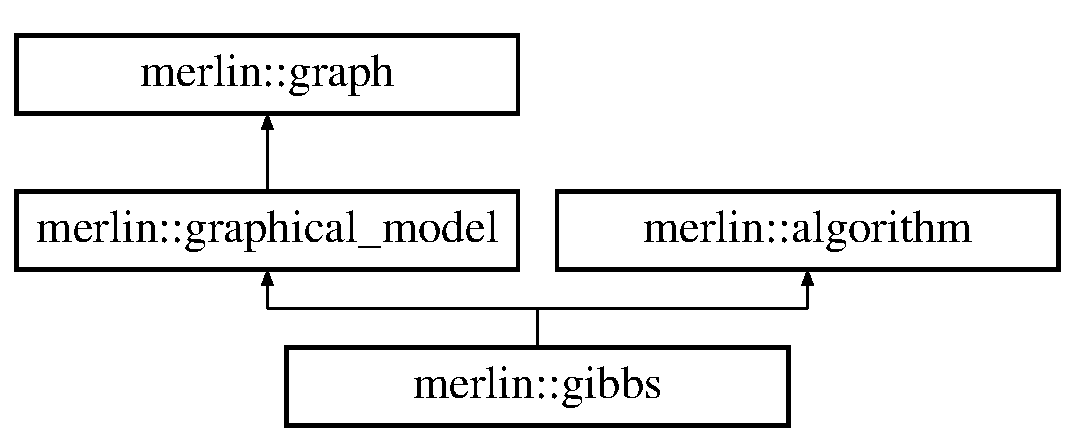
\includegraphics[height=3.000000cm]{classmerlin_1_1gibbs}
\end{center}
\end{figure}
\subsection*{Public Types}
\begin{DoxyCompactItemize}
\item 
typedef \hyperlink{classmerlin_1_1graphical__model_ab2b46f09d8142bb68f243ecadbdabb6b}{graphical\+\_\+model\+::findex} \hyperlink{classmerlin_1_1gibbs_a19c11865cd36a9920aec11f902958b93}{findex}\hypertarget{classmerlin_1_1gibbs_a19c11865cd36a9920aec11f902958b93}{}\label{classmerlin_1_1gibbs_a19c11865cd36a9920aec11f902958b93}

\begin{DoxyCompactList}\small\item\em Factor index. \end{DoxyCompactList}\item 
typedef \hyperlink{classmerlin_1_1graphical__model_a275006a490bc09239c12a4d93d53b135}{graphical\+\_\+model\+::vindex} \hyperlink{classmerlin_1_1gibbs_a6bfd73700f9e6917f89ea5c7894c7a5d}{vindex}\hypertarget{classmerlin_1_1gibbs_a6bfd73700f9e6917f89ea5c7894c7a5d}{}\label{classmerlin_1_1gibbs_a6bfd73700f9e6917f89ea5c7894c7a5d}

\begin{DoxyCompactList}\small\item\em Variable index. \end{DoxyCompactList}\item 
typedef \hyperlink{classmerlin_1_1graphical__model_a615e25ec6594615fddfd4c3c4776b99f}{graphical\+\_\+model\+::flist} \hyperlink{classmerlin_1_1gibbs_ae98b71f43cbaadae19535d4728225c06}{flist}\hypertarget{classmerlin_1_1gibbs_ae98b71f43cbaadae19535d4728225c06}{}\label{classmerlin_1_1gibbs_ae98b71f43cbaadae19535d4728225c06}

\begin{DoxyCompactList}\small\item\em Collection of factor indices. \end{DoxyCompactList}\end{DoxyCompactItemize}
\subsection*{Public Member Functions}
\begin{DoxyCompactItemize}
\item 
\hyperlink{classmerlin_1_1gibbs_a1513d2c6b58be4e4dd0e31c66d948e20}{gibbs} ()\hypertarget{classmerlin_1_1gibbs_a1513d2c6b58be4e4dd0e31c66d948e20}{}\label{classmerlin_1_1gibbs_a1513d2c6b58be4e4dd0e31c66d948e20}

\begin{DoxyCompactList}\small\item\em Creates an empty Gibbs sampler. \end{DoxyCompactList}\item 
\hyperlink{classmerlin_1_1gibbs_accbce95053cf0e18167d863ca9d3b832}{gibbs} (const \hyperlink{classmerlin_1_1graphical__model}{graphical\+\_\+model} \&fg)\hypertarget{classmerlin_1_1gibbs_accbce95053cf0e18167d863ca9d3b832}{}\label{classmerlin_1_1gibbs_accbce95053cf0e18167d863ca9d3b832}

\begin{DoxyCompactList}\small\item\em Creates a Gibbs sampler from an existing graphical model. \end{DoxyCompactList}\item 
\hyperlink{classmerlin_1_1gibbs}{gibbs} $\ast$ \hyperlink{classmerlin_1_1gibbs_a3479cca656a53a22c32ecdaa1a010308}{clone} () const 
\begin{DoxyCompactList}\small\item\em Clone the Gibbs sampler. \end{DoxyCompactList}\item 
\hyperlink{classmerlin_1_1gibbs_a323edb9ecc0c7c69ca872ec92f5d727c}{M\+E\+R\+\_\+\+E\+N\+UM} (Property, Task, Temp\+Min, Temp\+Max, Iter, Samples, Debug)\hypertarget{classmerlin_1_1gibbs_a323edb9ecc0c7c69ca872ec92f5d727c}{}\label{classmerlin_1_1gibbs_a323edb9ecc0c7c69ca872ec92f5d727c}

\begin{DoxyCompactList}\small\item\em Properties of the sampler. \end{DoxyCompactList}\item 
virtual void \hyperlink{classmerlin_1_1gibbs_ab3981d10b8a378c2979a1dbb58893df1}{set\+\_\+properties} (std\+::string opt=std\+::string())
\begin{DoxyCompactList}\small\item\em Set the properties of the sampler. \end{DoxyCompactList}\item 
void \hyperlink{classmerlin_1_1gibbs_ac14684f895fc27b59f318632a786acb7}{init} ()\hypertarget{classmerlin_1_1gibbs_ac14684f895fc27b59f318632a786acb7}{}\label{classmerlin_1_1gibbs_ac14684f895fc27b59f318632a786acb7}

\begin{DoxyCompactList}\small\item\em Initialize the Gibbs sampler. \end{DoxyCompactList}\item 
void \hyperlink{classmerlin_1_1gibbs_a2f9555aa3830e21e15a74c2ce7dc2109}{run} ()\hypertarget{classmerlin_1_1gibbs_a2f9555aa3830e21e15a74c2ce7dc2109}{}\label{classmerlin_1_1gibbs_a2f9555aa3830e21e15a74c2ce7dc2109}

\begin{DoxyCompactList}\small\item\em Run the Gibbs sampler. \end{DoxyCompactList}\item 
double \hyperlink{classmerlin_1_1gibbs_a560e770c1d7fe247e5fcb088cd00198c}{lb} () const 
\begin{DoxyCompactList}\small\item\em Lower bound on the optimal value. \end{DoxyCompactList}\item 
double \hyperlink{classmerlin_1_1gibbs_ac433bf8d912355ed96f4d2299f8d71d9}{ub} () const 
\begin{DoxyCompactList}\small\item\em Upper bound on the optimal value. \end{DoxyCompactList}\item 
std\+::vector$<$ \hyperlink{classmerlin_1_1graph_a5cade38832f47248573e921276f122d6}{index} $>$ \hyperlink{classmerlin_1_1gibbs_a10fd6e4e76f510f10a802e97584aff9e}{best\+\_\+config} () const 
\begin{DoxyCompactList}\small\item\em Best configuration. \end{DoxyCompactList}\item 
double \hyperlink{classmerlin_1_1gibbs_a2a57b5f7fa9571060e134164ca39c68f}{logZ} () const 
\begin{DoxyCompactList}\small\item\em Log value of the partition function. \end{DoxyCompactList}\item 
double \hyperlink{classmerlin_1_1gibbs_abfd6c9073faa8827b87acf333de77cd6}{log\+Zub} () const 
\begin{DoxyCompactList}\small\item\em Upper bound on the log partition function. \end{DoxyCompactList}\item 
double \hyperlink{classmerlin_1_1gibbs_ab4ee1ac60166f1e30b14e07a534aa4b8}{log\+Zlb} () const 
\begin{DoxyCompactList}\small\item\em Lower bound on the log partition function. \end{DoxyCompactList}\item 
const std\+::vector$<$ std\+::vector$<$ \hyperlink{classmerlin_1_1graph_a5cade38832f47248573e921276f122d6}{index} $>$ $>$ \& \hyperlink{classmerlin_1_1gibbs_a2b8c1231e5f9c770ab94d8bac275014a}{samples} ()\hypertarget{classmerlin_1_1gibbs_a2b8c1231e5f9c770ab94d8bac275014a}{}\label{classmerlin_1_1gibbs_a2b8c1231e5f9c770ab94d8bac275014a}

\begin{DoxyCompactList}\small\item\em Return the list of samples. \end{DoxyCompactList}\item 
const \hyperlink{classmerlin_1_1factor}{factor} \& \hyperlink{classmerlin_1_1gibbs_a578f69706383e3a29fabc65e8001b433}{belief} (size\+\_\+t i) const 
\begin{DoxyCompactList}\small\item\em Belief associated with a node of the graph. \end{DoxyCompactList}\item 
const \hyperlink{classmerlin_1_1factor}{factor} \& \hyperlink{classmerlin_1_1gibbs_aea5e692a62aee1fff134398565e85c6e}{belief} (\hyperlink{classmerlin_1_1variable}{variable} v) const 
\begin{DoxyCompactList}\small\item\em Belief associated with a particular variable. \end{DoxyCompactList}\item 
const \hyperlink{classmerlin_1_1factor}{factor} \& \hyperlink{classmerlin_1_1gibbs_af8b834f1ca8b2775a2a896b32442e303}{belief} (\hyperlink{classmerlin_1_1variable__set}{variable\+\_\+set} vs) const 
\begin{DoxyCompactList}\small\item\em Belief associated with a set of variables. \end{DoxyCompactList}\item 
const std\+::vector$<$ \hyperlink{classmerlin_1_1factor}{factor} $>$ \& \hyperlink{classmerlin_1_1gibbs_aae4b98aa02e5483d04fed2d9046c0900}{beliefs} () const 
\begin{DoxyCompactList}\small\item\em Beliefs associated with the variables. \end{DoxyCompactList}\item 
void \hyperlink{classmerlin_1_1gibbs_a33dabc870e830525a4bbf3b1559b8dd2}{write\+\_\+solution} (const char $\ast$file\+\_\+name, const std\+::map$<$ size\+\_\+t, size\+\_\+t $>$ \&evidence, const std\+::map$<$ size\+\_\+t, size\+\_\+t $>$ \&old2new, const \hyperlink{classmerlin_1_1graphical__model}{graphical\+\_\+model} \&orig)
\begin{DoxyCompactList}\small\item\em Write the solution to the output file. \end{DoxyCompactList}\item 
\hyperlink{classmerlin_1_1gibbs_ad764ab9776203f568dfdbd4ba9c4b928}{M\+E\+R\+\_\+\+E\+N\+UM} (Task, PR, M\+AR, M\+AP)\hypertarget{classmerlin_1_1gibbs_ad764ab9776203f568dfdbd4ba9c4b928}{}\label{classmerlin_1_1gibbs_ad764ab9776203f568dfdbd4ba9c4b928}

\begin{DoxyCompactList}\small\item\em Inference tasks supported. \end{DoxyCompactList}\end{DoxyCompactItemize}
\subsection*{Additional Inherited Members}


\subsection{Detailed Description}
Factor graph algorithm specialization for Gibbs sampling. 

Definition at line 37 of file gibbs.\+h.



\subsection{Member Function Documentation}
\index{merlin\+::gibbs@{merlin\+::gibbs}!belief@{belief}}
\index{belief@{belief}!merlin\+::gibbs@{merlin\+::gibbs}}
\subsubsection[{\texorpdfstring{belief(size\+\_\+t i) const }{belief(size_t i) const }}]{\setlength{\rightskip}{0pt plus 5cm}const {\bf factor}\& merlin\+::gibbs\+::belief (
\begin{DoxyParamCaption}
\item[{size\+\_\+t}]{i}
\end{DoxyParamCaption}
) const\hspace{0.3cm}{\ttfamily [inline]}, {\ttfamily [virtual]}}\hypertarget{classmerlin_1_1gibbs_a578f69706383e3a29fabc65e8001b433}{}\label{classmerlin_1_1gibbs_a578f69706383e3a29fabc65e8001b433}


Belief associated with a node of the graph. 

\begin{DoxyReturn}{Returns}
the belief associated with a node of the graph. Nodes correspond typically to variables. The belied is a function represented by the Factor class. 
\end{DoxyReturn}

\begin{DoxyParams}{Parameters}
{\em i} & The index of the node in the graph (from 0) \\
\hline
\end{DoxyParams}


Implements \hyperlink{classmerlin_1_1algorithm_a617b3e562037a7716f7cfd6cf1e55c19}{merlin\+::algorithm}.



Definition at line 304 of file gibbs.\+h.



Referenced by belief(), run(), and write\+\_\+solution().

\index{merlin\+::gibbs@{merlin\+::gibbs}!belief@{belief}}
\index{belief@{belief}!merlin\+::gibbs@{merlin\+::gibbs}}
\subsubsection[{\texorpdfstring{belief(variable v) const }{belief(variable v) const }}]{\setlength{\rightskip}{0pt plus 5cm}const {\bf factor}\& merlin\+::gibbs\+::belief (
\begin{DoxyParamCaption}
\item[{{\bf variable}}]{v}
\end{DoxyParamCaption}
) const\hspace{0.3cm}{\ttfamily [inline]}, {\ttfamily [virtual]}}\hypertarget{classmerlin_1_1gibbs_aea5e692a62aee1fff134398565e85c6e}{}\label{classmerlin_1_1gibbs_aea5e692a62aee1fff134398565e85c6e}


Belief associated with a particular variable. 


\begin{DoxyParams}{Parameters}
{\em v} & The variable to compute the belief of \\
\hline
\end{DoxyParams}
\begin{DoxyReturn}{Returns}
the belief associated with a particular variable in the graphical model. The belief is a function represented by the Factor class. 
\end{DoxyReturn}


Implements \hyperlink{classmerlin_1_1algorithm_adc966d1ed7ac479754441bab138f7efa}{merlin\+::algorithm}.



Definition at line 307 of file gibbs.\+h.



References belief(), and merlin\+::graphical\+\_\+model\+::with\+\_\+variable().

\index{merlin\+::gibbs@{merlin\+::gibbs}!belief@{belief}}
\index{belief@{belief}!merlin\+::gibbs@{merlin\+::gibbs}}
\subsubsection[{\texorpdfstring{belief(variable\+\_\+set vs) const }{belief(variable_set vs) const }}]{\setlength{\rightskip}{0pt plus 5cm}const {\bf factor}\& merlin\+::gibbs\+::belief (
\begin{DoxyParamCaption}
\item[{{\bf variable\+\_\+set}}]{vs}
\end{DoxyParamCaption}
) const\hspace{0.3cm}{\ttfamily [inline]}, {\ttfamily [virtual]}}\hypertarget{classmerlin_1_1gibbs_af8b834f1ca8b2775a2a896b32442e303}{}\label{classmerlin_1_1gibbs_af8b834f1ca8b2775a2a896b32442e303}


Belief associated with a set of variables. 


\begin{DoxyParams}{Parameters}
{\em vs} & The set of variables to compute the belief of \\
\hline
\end{DoxyParams}
\begin{DoxyReturn}{Returns}
the belief associated with a set of variables in the graphical model. The belief is a function represented by the Factor class. 
\end{DoxyReturn}


Implements \hyperlink{classmerlin_1_1algorithm_ad19b068623b85ad1cd4bb262e7bcfc6f}{merlin\+::algorithm}.



Definition at line 310 of file gibbs.\+h.

\index{merlin\+::gibbs@{merlin\+::gibbs}!beliefs@{beliefs}}
\index{beliefs@{beliefs}!merlin\+::gibbs@{merlin\+::gibbs}}
\subsubsection[{\texorpdfstring{beliefs() const }{beliefs() const }}]{\setlength{\rightskip}{0pt plus 5cm}const std\+::vector$<${\bf factor}$>$\& merlin\+::gibbs\+::beliefs (
\begin{DoxyParamCaption}
{}
\end{DoxyParamCaption}
) const\hspace{0.3cm}{\ttfamily [inline]}, {\ttfamily [virtual]}}\hypertarget{classmerlin_1_1gibbs_aae4b98aa02e5483d04fed2d9046c0900}{}\label{classmerlin_1_1gibbs_aae4b98aa02e5483d04fed2d9046c0900}


Beliefs associated with the variables. 

\begin{DoxyReturn}{Returns}
the beliefs associated with the variables in the graphical model (one belief for each of the variables). The output vector is indexed by the same indexes used for the variables. 
\end{DoxyReturn}


Implements \hyperlink{classmerlin_1_1algorithm_a0b70d8fe87b32bca601a3d116b673b47}{merlin\+::algorithm}.



Definition at line 313 of file gibbs.\+h.

\index{merlin\+::gibbs@{merlin\+::gibbs}!best\+\_\+config@{best\+\_\+config}}
\index{best\+\_\+config@{best\+\_\+config}!merlin\+::gibbs@{merlin\+::gibbs}}
\subsubsection[{\texorpdfstring{best\+\_\+config() const }{best_config() const }}]{\setlength{\rightskip}{0pt plus 5cm}std\+::vector$<${\bf index}$>$ merlin\+::gibbs\+::best\+\_\+config (
\begin{DoxyParamCaption}
{}
\end{DoxyParamCaption}
) const\hspace{0.3cm}{\ttfamily [inline]}, {\ttfamily [virtual]}}\hypertarget{classmerlin_1_1gibbs_a10fd6e4e76f510f10a802e97584aff9e}{}\label{classmerlin_1_1gibbs_a10fd6e4e76f510f10a802e97584aff9e}


Best configuration. 

\begin{DoxyReturn}{Returns}
a vector containing the best configuration of the variables (i.\+e., variable value assignments) found so far. It is specific to optimization tasks (e.\+g., M\+AP, Marginal M\+AP). 
\end{DoxyReturn}


Implements \hyperlink{classmerlin_1_1algorithm_a3d84d2595e6235db93a9bb3e1a012e48}{merlin\+::algorithm}.



Definition at line 284 of file gibbs.\+h.

\index{merlin\+::gibbs@{merlin\+::gibbs}!clone@{clone}}
\index{clone@{clone}!merlin\+::gibbs@{merlin\+::gibbs}}
\subsubsection[{\texorpdfstring{clone() const }{clone() const }}]{\setlength{\rightskip}{0pt plus 5cm}{\bf gibbs}$\ast$ merlin\+::gibbs\+::clone (
\begin{DoxyParamCaption}
{}
\end{DoxyParamCaption}
) const\hspace{0.3cm}{\ttfamily [inline]}, {\ttfamily [virtual]}}\hypertarget{classmerlin_1_1gibbs_a3479cca656a53a22c32ecdaa1a010308}{}\label{classmerlin_1_1gibbs_a3479cca656a53a22c32ecdaa1a010308}


Clone the Gibbs sampler. 

\begin{DoxyReturn}{Returns}
the pointer to the cloned sampler. 
\end{DoxyReturn}


Implements \hyperlink{classmerlin_1_1algorithm_a10f787e24c1fd5ec92c26b18efb0b8db}{merlin\+::algorithm}.



Definition at line 65 of file gibbs.\+h.



References gibbs(), and M\+E\+R\+\_\+\+E\+N\+U\+M().

\index{merlin\+::gibbs@{merlin\+::gibbs}!lb@{lb}}
\index{lb@{lb}!merlin\+::gibbs@{merlin\+::gibbs}}
\subsubsection[{\texorpdfstring{lb() const }{lb() const }}]{\setlength{\rightskip}{0pt plus 5cm}double merlin\+::gibbs\+::lb (
\begin{DoxyParamCaption}
{}
\end{DoxyParamCaption}
) const\hspace{0.3cm}{\ttfamily [inline]}, {\ttfamily [virtual]}}\hypertarget{classmerlin_1_1gibbs_a560e770c1d7fe247e5fcb088cd00198c}{}\label{classmerlin_1_1gibbs_a560e770c1d7fe247e5fcb088cd00198c}


Lower bound on the optimal value. 

\begin{DoxyReturn}{Returns}
a lower bound on the optimal value defined by the inference task if available. 
\end{DoxyReturn}


Implements \hyperlink{classmerlin_1_1algorithm_adc3f19055c0466682b5577049df14863}{merlin\+::algorithm}.



Definition at line 278 of file gibbs.\+h.

\index{merlin\+::gibbs@{merlin\+::gibbs}!logZ@{logZ}}
\index{logZ@{logZ}!merlin\+::gibbs@{merlin\+::gibbs}}
\subsubsection[{\texorpdfstring{log\+Z() const }{logZ() const }}]{\setlength{\rightskip}{0pt plus 5cm}double merlin\+::gibbs\+::logZ (
\begin{DoxyParamCaption}
{}
\end{DoxyParamCaption}
) const\hspace{0.3cm}{\ttfamily [inline]}, {\ttfamily [virtual]}}\hypertarget{classmerlin_1_1gibbs_a2a57b5f7fa9571060e134164ca39c68f}{}\label{classmerlin_1_1gibbs_a2a57b5f7fa9571060e134164ca39c68f}


Log value of the partition function. 

\begin{DoxyReturn}{Returns}
an estimate the log parition function. If the inference algorithm is an exact one then the return value is the exact log value of the partition function. 
\end{DoxyReturn}


Implements \hyperlink{classmerlin_1_1algorithm_a26eadf71ba80c0a9cd3d7cfe18c95717}{merlin\+::algorithm}.



Definition at line 287 of file gibbs.\+h.

\index{merlin\+::gibbs@{merlin\+::gibbs}!log\+Zlb@{log\+Zlb}}
\index{log\+Zlb@{log\+Zlb}!merlin\+::gibbs@{merlin\+::gibbs}}
\subsubsection[{\texorpdfstring{log\+Zlb() const }{logZlb() const }}]{\setlength{\rightskip}{0pt plus 5cm}double merlin\+::gibbs\+::log\+Zlb (
\begin{DoxyParamCaption}
{}
\end{DoxyParamCaption}
) const\hspace{0.3cm}{\ttfamily [inline]}, {\ttfamily [virtual]}}\hypertarget{classmerlin_1_1gibbs_ab4ee1ac60166f1e30b14e07a534aa4b8}{}\label{classmerlin_1_1gibbs_ab4ee1ac60166f1e30b14e07a534aa4b8}


Lower bound on the log partition function. 

\begin{DoxyReturn}{Returns}
a lower bound on the log value of the parition function. 
\end{DoxyReturn}


Implements \hyperlink{classmerlin_1_1algorithm_a14d163a3e90a898487d3a6e273e1fecf}{merlin\+::algorithm}.



Definition at line 293 of file gibbs.\+h.

\index{merlin\+::gibbs@{merlin\+::gibbs}!log\+Zub@{log\+Zub}}
\index{log\+Zub@{log\+Zub}!merlin\+::gibbs@{merlin\+::gibbs}}
\subsubsection[{\texorpdfstring{log\+Zub() const }{logZub() const }}]{\setlength{\rightskip}{0pt plus 5cm}double merlin\+::gibbs\+::log\+Zub (
\begin{DoxyParamCaption}
{}
\end{DoxyParamCaption}
) const\hspace{0.3cm}{\ttfamily [inline]}, {\ttfamily [virtual]}}\hypertarget{classmerlin_1_1gibbs_abfd6c9073faa8827b87acf333de77cd6}{}\label{classmerlin_1_1gibbs_abfd6c9073faa8827b87acf333de77cd6}


Upper bound on the log partition function. 

\begin{DoxyReturn}{Returns}
an upper bound on the log value of the parition function. Most inference algorithms implemented in merlin support upper bounds on the log partition function. 
\end{DoxyReturn}


Implements \hyperlink{classmerlin_1_1algorithm_aeece2e8f008bcc94697353088c4afefe}{merlin\+::algorithm}.



Definition at line 290 of file gibbs.\+h.

\index{merlin\+::gibbs@{merlin\+::gibbs}!set\+\_\+properties@{set\+\_\+properties}}
\index{set\+\_\+properties@{set\+\_\+properties}!merlin\+::gibbs@{merlin\+::gibbs}}
\subsubsection[{\texorpdfstring{set\+\_\+properties(std\+::string opt=std\+::string())}{set_properties(std::string opt=std::string())}}]{\setlength{\rightskip}{0pt plus 5cm}virtual void merlin\+::gibbs\+::set\+\_\+properties (
\begin{DoxyParamCaption}
\item[{std\+::string}]{opt = {\ttfamily std\+:\+:string()}}
\end{DoxyParamCaption}
)\hspace{0.3cm}{\ttfamily [inline]}, {\ttfamily [virtual]}}\hypertarget{classmerlin_1_1gibbs_ab3981d10b8a378c2979a1dbb58893df1}{}\label{classmerlin_1_1gibbs_ab3981d10b8a378c2979a1dbb58893df1}


Set the properties of the sampler. 


\begin{DoxyParams}{Parameters}
{\em opt} & The string of comma separated property value pairs \\
\hline
\end{DoxyParams}


Definition at line 79 of file gibbs.\+h.



References merlin\+::graphical\+\_\+model\+::nvar().



Referenced by gibbs(), and Merlin\+::run().

\index{merlin\+::gibbs@{merlin\+::gibbs}!ub@{ub}}
\index{ub@{ub}!merlin\+::gibbs@{merlin\+::gibbs}}
\subsubsection[{\texorpdfstring{ub() const }{ub() const }}]{\setlength{\rightskip}{0pt plus 5cm}double merlin\+::gibbs\+::ub (
\begin{DoxyParamCaption}
{}
\end{DoxyParamCaption}
) const\hspace{0.3cm}{\ttfamily [inline]}, {\ttfamily [virtual]}}\hypertarget{classmerlin_1_1gibbs_ac433bf8d912355ed96f4d2299f8d71d9}{}\label{classmerlin_1_1gibbs_ac433bf8d912355ed96f4d2299f8d71d9}


Upper bound on the optimal value. 

\begin{DoxyReturn}{Returns}
an upper bound on the optimal value defined by the inference task. It is specific to optimization tasks such as M\+AP and Marginal M\+AP inference. 
\end{DoxyReturn}


Implements \hyperlink{classmerlin_1_1algorithm_a2698bb69f5559889d4903a640f08cd66}{merlin\+::algorithm}.



Definition at line 281 of file gibbs.\+h.

\index{merlin\+::gibbs@{merlin\+::gibbs}!write\+\_\+solution@{write\+\_\+solution}}
\index{write\+\_\+solution@{write\+\_\+solution}!merlin\+::gibbs@{merlin\+::gibbs}}
\subsubsection[{\texorpdfstring{write\+\_\+solution(const char $\ast$file\+\_\+name, const std\+::map$<$ size\+\_\+t, size\+\_\+t $>$ \&evidence, const std\+::map$<$ size\+\_\+t, size\+\_\+t $>$ \&old2new, const graphical\+\_\+model \&orig)}{write_solution(const char *file_name, const std::map< size_t, size_t > &evidence, const std::map< size_t, size_t > &old2new, const graphical_model &orig)}}]{\setlength{\rightskip}{0pt plus 5cm}void merlin\+::gibbs\+::write\+\_\+solution (
\begin{DoxyParamCaption}
\item[{const char $\ast$}]{file\+\_\+name, }
\item[{const std\+::map$<$ size\+\_\+t, size\+\_\+t $>$ \&}]{evidence, }
\item[{const std\+::map$<$ size\+\_\+t, size\+\_\+t $>$ \&}]{old2new, }
\item[{const {\bf graphical\+\_\+model} \&}]{orig}
\end{DoxyParamCaption}
)\hspace{0.3cm}{\ttfamily [inline]}}\hypertarget{classmerlin_1_1gibbs_a33dabc870e830525a4bbf3b1559b8dd2}{}\label{classmerlin_1_1gibbs_a33dabc870e830525a4bbf3b1559b8dd2}


Write the solution to the output file. 


\begin{DoxyParams}{Parameters}
{\em filename} & The output file name \\
\hline
{\em evidence} & The evidence variable value pairs \\
\hline
{\em old2new} & The mapping between old and new variable indexing \\
\hline
{\em orig} & The graphical model prior to asserting evidence \\
\hline
\end{DoxyParams}


Definition at line 325 of file gibbs.\+h.



References belief(), M\+E\+R\+\_\+\+E\+N\+U\+M(), merlin\+::graphical\+\_\+model\+::nvar(), merlin\+::variable\+::states(), and merlin\+::graphical\+\_\+model\+::var().



Referenced by Merlin\+::run().



The documentation for this class was generated from the following file\+:\begin{DoxyCompactItemize}
\item 
src/include/\hyperlink{gibbs_8h}{gibbs.\+h}\end{DoxyCompactItemize}

\hypertarget{classmerlin_1_1graph}{}\section{merlin\+:\+:graph Class Reference}
\label{classmerlin_1_1graph}\index{merlin\+::graph@{merlin\+::graph}}


The graph structure used by \hyperlink{classMerlin}{Merlin}.  




{\ttfamily \#include $<$graph.\+h$>$}

Inheritance diagram for merlin\+:\+:graph\+:\begin{figure}[H]
\begin{center}
\leavevmode
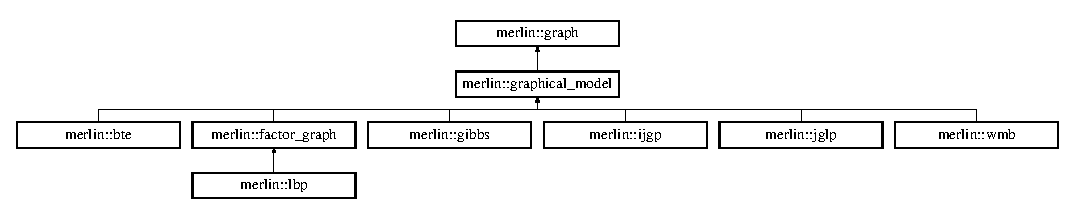
\includegraphics[height=2.440087cm]{classmerlin_1_1graph}
\end{center}
\end{figure}
\subsection*{Public Types}
\begin{DoxyCompactItemize}
\item 
typedef \hyperlink{structmerlin_1_1edge__id_af57e3c1f2c2c3194d96468a5f0e7cce0}{edge\+\_\+id\+::index} \hyperlink{classmerlin_1_1graph_a5cade38832f47248573e921276f122d6}{index}\hypertarget{classmerlin_1_1graph_a5cade38832f47248573e921276f122d6}{}\label{classmerlin_1_1graph_a5cade38832f47248573e921276f122d6}

\begin{DoxyCompactList}\small\item\em Basic indexing type for the graph. \end{DoxyCompactList}\end{DoxyCompactItemize}
\subsection*{Public Member Functions}
\begin{DoxyCompactItemize}
\item 
\hyperlink{classmerlin_1_1graph_aa01a823270b0fb2edbc2cd6622e961fe}{graph} (size\+\_\+t n=0)
\begin{DoxyCompactList}\small\item\em Constructs a graph with {\itshape n} vertices and 0 edges. \end{DoxyCompactList}\item 
\hyperlink{classmerlin_1_1graph_a6c24adfdbf5091e0adea5c2bf551debc}{$\sim$graph} ()\hypertarget{classmerlin_1_1graph_a6c24adfdbf5091e0adea5c2bf551debc}{}\label{classmerlin_1_1graph_a6c24adfdbf5091e0adea5c2bf551debc}

\begin{DoxyCompactList}\small\item\em Destroys the graph. \end{DoxyCompactList}\item 
\hyperlink{classmerlin_1_1graph_a5cade38832f47248573e921276f122d6}{index} \hyperlink{classmerlin_1_1graph_a844faa05514a364e89c53cef10e59a9b}{add\+\_\+node} ()
\begin{DoxyCompactList}\small\item\em Add a node to the graph. \end{DoxyCompactList}\item 
void \hyperlink{classmerlin_1_1graph_a33a6ba0779fcd5a432eb0e9fade5113e}{remove\+\_\+node} (\hyperlink{classmerlin_1_1graph_a5cade38832f47248573e921276f122d6}{index} i)
\begin{DoxyCompactList}\small\item\em Remove a node from the graph. \end{DoxyCompactList}\item 
size\+\_\+t \hyperlink{classmerlin_1_1graph_a068fcb26500eccd201a6ca877d76fafe}{num\+\_\+nodes} ()\hypertarget{classmerlin_1_1graph_a068fcb26500eccd201a6ca877d76fafe}{}\label{classmerlin_1_1graph_a068fcb26500eccd201a6ca877d76fafe}

\begin{DoxyCompactList}\small\item\em Return the number of nodes. \end{DoxyCompactList}\item 
size\+\_\+t \hyperlink{classmerlin_1_1graph_a2d2debc5137f505ce83009067d125b5d}{num\+\_\+edges} ()\hypertarget{classmerlin_1_1graph_a2d2debc5137f505ce83009067d125b5d}{}\label{classmerlin_1_1graph_a2d2debc5137f505ce83009067d125b5d}

\begin{DoxyCompactList}\small\item\em Return the number of edges. \end{DoxyCompactList}\item 
const \hyperlink{structmerlin_1_1edge__id}{edge\+\_\+id} \& \hyperlink{classmerlin_1_1graph_abb6ac50bdc67b24c70ac9cb896475350}{add\+\_\+edge} (\hyperlink{classmerlin_1_1graph_a5cade38832f47248573e921276f122d6}{index} i, \hyperlink{classmerlin_1_1graph_a5cade38832f47248573e921276f122d6}{index} j)
\begin{DoxyCompactList}\small\item\em Add an edge to the graph. \end{DoxyCompactList}\item 
void \hyperlink{classmerlin_1_1graph_a1d17b17fbf5b8378c1d65b885e688897}{remove\+\_\+edge} (\hyperlink{classmerlin_1_1graph_a5cade38832f47248573e921276f122d6}{index} i, \hyperlink{classmerlin_1_1graph_a5cade38832f47248573e921276f122d6}{index} j)
\begin{DoxyCompactList}\small\item\em Remove an edge from the graph. \end{DoxyCompactList}\item 
void \hyperlink{classmerlin_1_1graph_a1971a84f3b1b32af0a4eeff502c491e3}{clear} ()\hypertarget{classmerlin_1_1graph_a1971a84f3b1b32af0a4eeff502c491e3}{}\label{classmerlin_1_1graph_a1971a84f3b1b32af0a4eeff502c491e3}

\begin{DoxyCompactList}\small\item\em Clear the graph by removing all nodes and edges. \end{DoxyCompactList}\item 
void \hyperlink{classmerlin_1_1graph_a1c405b536daed8d6f4f4ca49b0e93834}{clear\+\_\+edges} ()\hypertarget{classmerlin_1_1graph_a1c405b536daed8d6f4f4ca49b0e93834}{}\label{classmerlin_1_1graph_a1c405b536daed8d6f4f4ca49b0e93834}

\begin{DoxyCompactList}\small\item\em Remove all edges. \end{DoxyCompactList}\item 
const \hyperlink{structmerlin_1_1edge__id}{edge\+\_\+id} \& \hyperlink{classmerlin_1_1graph_ac245de085fc9a8b34a6dd3bf9459815d}{edge} (\hyperlink{classmerlin_1_1graph_a5cade38832f47248573e921276f122d6}{index} i, \hyperlink{classmerlin_1_1graph_a5cade38832f47248573e921276f122d6}{index} j) const 
\begin{DoxyCompactList}\small\item\em Return the edge (if any) between two nodes. \end{DoxyCompactList}\item 
const \hyperlink{classmerlin_1_1set}{set}$<$ \hyperlink{structmerlin_1_1edge__id}{edge\+\_\+id} $>$ \& \hyperlink{classmerlin_1_1graph_a3681cb03e7596b425b6b5641ba5d6404}{neighbors} (\hyperlink{classmerlin_1_1graph_a5cade38832f47248573e921276f122d6}{index} i) const 
\begin{DoxyCompactList}\small\item\em Return the neighbors of a node (ie, adjacency list). \end{DoxyCompactList}\item 
const \hyperlink{structmerlin_1_1edge__id}{edge\+\_\+id} \& \hyperlink{classmerlin_1_1graph_adfb67c1cfa94e88a90b9708607bcacb0}{edge} (\hyperlink{classmerlin_1_1graph_a5cade38832f47248573e921276f122d6}{index} eij) const 
\begin{DoxyCompactList}\small\item\em Return an edge (by its index). \end{DoxyCompactList}\item 
const std\+::vector$<$ \hyperlink{structmerlin_1_1edge__id}{edge\+\_\+id} $>$ \& \hyperlink{classmerlin_1_1graph_ab1d18f639ac9e5eb08061c8c011916f0}{edges} () const 
\begin{DoxyCompactList}\small\item\em Return the edges of the graph. \end{DoxyCompactList}\end{DoxyCompactItemize}
\subsection*{Public Attributes}
\begin{DoxyCompactItemize}
\item 
std\+::vector$<$ \hyperlink{classmerlin_1_1set}{set}$<$ \hyperlink{structmerlin_1_1edge__id}{edge\+\_\+id} $>$ $>$ \hyperlink{classmerlin_1_1graph_a71cf7768aa72159f3ae7b52ef6b23993}{m\+\_\+adj}\hypertarget{classmerlin_1_1graph_a71cf7768aa72159f3ae7b52ef6b23993}{}\label{classmerlin_1_1graph_a71cf7768aa72159f3ae7b52ef6b23993}

\begin{DoxyCompactList}\small\item\em Look up Edge\+ID info by adj\mbox{[}i\mbox{]}\mbox{[}jj\mbox{]} (jj = position of j). \end{DoxyCompactList}\item 
std\+::vector$<$ \hyperlink{structmerlin_1_1edge__id}{edge\+\_\+id} $>$ \hyperlink{classmerlin_1_1graph_a6ff5b1d6713ff82d50f9888f2b60390f}{m\+\_\+edges}\hypertarget{classmerlin_1_1graph_a6ff5b1d6713ff82d50f9888f2b60390f}{}\label{classmerlin_1_1graph_a6ff5b1d6713ff82d50f9888f2b60390f}

\begin{DoxyCompactList}\small\item\em Look up Edge\+ID info by edges\mbox{[}eij\mbox{]} (edge index). \end{DoxyCompactList}\end{DoxyCompactItemize}
\subsection*{Protected Attributes}
\begin{DoxyCompactItemize}
\item 
std\+::stack$<$ \hyperlink{classmerlin_1_1graph_a5cade38832f47248573e921276f122d6}{index} $>$ \hyperlink{classmerlin_1_1graph_a6b3ab6e44183a8b27bb04f93166fbffb}{m\+\_\+vvacant}\hypertarget{classmerlin_1_1graph_a6b3ab6e44183a8b27bb04f93166fbffb}{}\label{classmerlin_1_1graph_a6b3ab6e44183a8b27bb04f93166fbffb}

\begin{DoxyCompactList}\small\item\em List of available vertex ids. \end{DoxyCompactList}\item 
std\+::stack$<$ \hyperlink{classmerlin_1_1graph_a5cade38832f47248573e921276f122d6}{index} $>$ \hyperlink{classmerlin_1_1graph_a9ebdd8a3cfe95f6159759c41836bf495}{m\+\_\+evacant}\hypertarget{classmerlin_1_1graph_a9ebdd8a3cfe95f6159759c41836bf495}{}\label{classmerlin_1_1graph_a9ebdd8a3cfe95f6159759c41836bf495}

\begin{DoxyCompactList}\small\item\em List of available edge ids. \end{DoxyCompactList}\end{DoxyCompactItemize}


\subsection{Detailed Description}
The graph structure used by \hyperlink{classMerlin}{Merlin}. 

The graph contains N {\itshape nodes} (indexed 0..N-\/1) and E {\itshape edges}, with bidirectional indexing (0..2\+E-\/1). 

Definition at line 106 of file graph.\+h.



\subsection{Constructor \& Destructor Documentation}
\index{merlin\+::graph@{merlin\+::graph}!graph@{graph}}
\index{graph@{graph}!merlin\+::graph@{merlin\+::graph}}
\subsubsection[{\texorpdfstring{graph(size\+\_\+t n=0)}{graph(size_t n=0)}}]{\setlength{\rightskip}{0pt plus 5cm}merlin\+::graph\+::graph (
\begin{DoxyParamCaption}
\item[{size\+\_\+t}]{n = {\ttfamily 0}}
\end{DoxyParamCaption}
)\hspace{0.3cm}{\ttfamily [inline]}, {\ttfamily [explicit]}}\hypertarget{classmerlin_1_1graph_aa01a823270b0fb2edbc2cd6622e961fe}{}\label{classmerlin_1_1graph_aa01a823270b0fb2edbc2cd6622e961fe}


Constructs a graph with {\itshape n} vertices and 0 edges. 


\begin{DoxyParams}{Parameters}
{\em n} & The number of nodes \\
\hline
\end{DoxyParams}


Definition at line 121 of file graph.\+h.



\subsection{Member Function Documentation}
\index{merlin\+::graph@{merlin\+::graph}!add\+\_\+edge@{add\+\_\+edge}}
\index{add\+\_\+edge@{add\+\_\+edge}!merlin\+::graph@{merlin\+::graph}}
\subsubsection[{\texorpdfstring{add\+\_\+edge(index i, index j)}{add_edge(index i, index j)}}]{\setlength{\rightskip}{0pt plus 5cm}const {\bf edge\+\_\+id}\& merlin\+::graph\+::add\+\_\+edge (
\begin{DoxyParamCaption}
\item[{{\bf index}}]{i, }
\item[{{\bf index}}]{j}
\end{DoxyParamCaption}
)\hspace{0.3cm}{\ttfamily [inline]}}\hypertarget{classmerlin_1_1graph_abb6ac50bdc67b24c70ac9cb896475350}{}\label{classmerlin_1_1graph_abb6ac50bdc67b24c70ac9cb896475350}


Add an edge to the graph. 

Create the pairs (i,j) and (j,i) in the adjacency list. 
\begin{DoxyParams}{Parameters}
{\em i} & The head of the edge \\
\hline
{\em j} & The tail of the edge \\
\hline
\end{DoxyParams}
\begin{DoxyReturn}{Returns}
the id (index) of the newly added edge. 
\end{DoxyReturn}


Definition at line 176 of file graph.\+h.



References merlin\+::edge\+\_\+id\+::edge\+\_\+id(), and merlin\+::edge\+\_\+id\+::\+N\+O\+\_\+\+E\+D\+GE.



Referenced by merlin\+::factor\+\_\+graph\+::add\+\_\+factor(), merlin\+::factor\+\_\+graph\+::create\+\_\+factor\+\_\+graph(), merlin\+::graphical\+\_\+model\+::induced\+\_\+width(), merlin\+::bte\+::init(), merlin\+::ijgp\+::init(), merlin\+::wmb\+::init(), merlin\+::graphical\+\_\+model\+::order2(), and merlin\+::jglp\+::run().

\index{merlin\+::graph@{merlin\+::graph}!add\+\_\+node@{add\+\_\+node}}
\index{add\+\_\+node@{add\+\_\+node}!merlin\+::graph@{merlin\+::graph}}
\subsubsection[{\texorpdfstring{add\+\_\+node()}{add_node()}}]{\setlength{\rightskip}{0pt plus 5cm}{\bf index} merlin\+::graph\+::add\+\_\+node (
\begin{DoxyParamCaption}
{}
\end{DoxyParamCaption}
)\hspace{0.3cm}{\ttfamily [inline]}}\hypertarget{classmerlin_1_1graph_a844faa05514a364e89c53cef10e59a9b}{}\label{classmerlin_1_1graph_a844faa05514a364e89c53cef10e59a9b}


Add a node to the graph. 

\begin{DoxyReturn}{Returns}
the index of the newly added node. 
\end{DoxyReturn}


Definition at line 135 of file graph.\+h.



Referenced by merlin\+::graphical\+\_\+model\+::add\+\_\+factor(), and merlin\+::graphical\+\_\+model\+::fixup().

\index{merlin\+::graph@{merlin\+::graph}!edge@{edge}}
\index{edge@{edge}!merlin\+::graph@{merlin\+::graph}}
\subsubsection[{\texorpdfstring{edge(index i, index j) const }{edge(index i, index j) const }}]{\setlength{\rightskip}{0pt plus 5cm}const {\bf edge\+\_\+id}\& merlin\+::graph\+::edge (
\begin{DoxyParamCaption}
\item[{{\bf index}}]{i, }
\item[{{\bf index}}]{j}
\end{DoxyParamCaption}
) const\hspace{0.3cm}{\ttfamily [inline]}}\hypertarget{classmerlin_1_1graph_ac245de085fc9a8b34a6dd3bf9459815d}{}\label{classmerlin_1_1graph_ac245de085fc9a8b34a6dd3bf9459815d}


Return the edge (if any) between two nodes. 


\begin{DoxyParams}{Parameters}
{\em i} & The head of the edge \\
\hline
{\em j} & The tail of the edge \\
\hline
\end{DoxyParams}
\begin{DoxyReturn}{Returns}
the index of the edge if the edge is present or the static constant N\+O\+\_\+\+E\+D\+GE if the edge is missing. 
\end{DoxyReturn}


Definition at line 248 of file graph.\+h.



References merlin\+::edge\+\_\+id\+::edge\+\_\+id(), and merlin\+::edge\+\_\+id\+::\+N\+O\+\_\+\+E\+D\+GE.



Referenced by merlin\+::factor\+\_\+graph\+::\+\_\+eindex(), merlin\+::lbp\+::init(), merlin\+::graphical\+\_\+model\+::order\+\_\+score(), and merlin\+::lbp\+::run().

\index{merlin\+::graph@{merlin\+::graph}!edge@{edge}}
\index{edge@{edge}!merlin\+::graph@{merlin\+::graph}}
\subsubsection[{\texorpdfstring{edge(index eij) const }{edge(index eij) const }}]{\setlength{\rightskip}{0pt plus 5cm}const {\bf edge\+\_\+id}\& merlin\+::graph\+::edge (
\begin{DoxyParamCaption}
\item[{{\bf index}}]{eij}
\end{DoxyParamCaption}
) const\hspace{0.3cm}{\ttfamily [inline]}}\hypertarget{classmerlin_1_1graph_adfb67c1cfa94e88a90b9708607bcacb0}{}\label{classmerlin_1_1graph_adfb67c1cfa94e88a90b9708607bcacb0}


Return an edge (by its index). 


\begin{DoxyParams}{Parameters}
{\em eij} & The index of the edge \\
\hline
\end{DoxyParams}
\begin{DoxyReturn}{Returns}
the edge id corresponding to the index. 
\end{DoxyReturn}


Definition at line 268 of file graph.\+h.

\index{merlin\+::graph@{merlin\+::graph}!edges@{edges}}
\index{edges@{edges}!merlin\+::graph@{merlin\+::graph}}
\subsubsection[{\texorpdfstring{edges() const }{edges() const }}]{\setlength{\rightskip}{0pt plus 5cm}const std\+::vector$<${\bf edge\+\_\+id}$>$\& merlin\+::graph\+::edges (
\begin{DoxyParamCaption}
{}
\end{DoxyParamCaption}
) const\hspace{0.3cm}{\ttfamily [inline]}}\hypertarget{classmerlin_1_1graph_ab1d18f639ac9e5eb08061c8c011916f0}{}\label{classmerlin_1_1graph_ab1d18f639ac9e5eb08061c8c011916f0}


Return the edges of the graph. 

\begin{DoxyReturn}{Returns}
the list of all edge ids in the graph. 
\end{DoxyReturn}


Definition at line 276 of file graph.\+h.



Referenced by merlin\+::bte\+::init(), merlin\+::ijgp\+::init(), merlin\+::wmb\+::init(), and merlin\+::jglp\+::tighten().

\index{merlin\+::graph@{merlin\+::graph}!neighbors@{neighbors}}
\index{neighbors@{neighbors}!merlin\+::graph@{merlin\+::graph}}
\subsubsection[{\texorpdfstring{neighbors(index i) const }{neighbors(index i) const }}]{\setlength{\rightskip}{0pt plus 5cm}const {\bf set}$<${\bf edge\+\_\+id}$>$\& merlin\+::graph\+::neighbors (
\begin{DoxyParamCaption}
\item[{{\bf index}}]{i}
\end{DoxyParamCaption}
) const\hspace{0.3cm}{\ttfamily [inline]}}\hypertarget{classmerlin_1_1graph_a3681cb03e7596b425b6b5641ba5d6404}{}\label{classmerlin_1_1graph_a3681cb03e7596b425b6b5641ba5d6404}


Return the neighbors of a node (ie, adjacency list). 


\begin{DoxyParams}{Parameters}
{\em i} & The index of the node \\
\hline
\end{DoxyParams}
\begin{DoxyReturn}{Returns}
the set of edge ids that are adjacent to the node. 
\end{DoxyReturn}


Definition at line 260 of file graph.\+h.



Referenced by merlin\+::factor\+\_\+graph\+::\+\_\+neighbors(), merlin\+::lbp\+::accept\+\_\+incoming(), merlin\+::lbp\+::calc\+\_\+belief(), merlin\+::graphical\+\_\+model\+::induced\+\_\+width(), merlin\+::lbp\+::init(), merlin\+::graphical\+\_\+model\+::order2(), merlin\+::graphical\+\_\+model\+::order\+\_\+score(), merlin\+::factor\+\_\+graph\+::span\+\_\+tree(), and merlin\+::lbp\+::update\+\_\+outgoing().

\index{merlin\+::graph@{merlin\+::graph}!remove\+\_\+edge@{remove\+\_\+edge}}
\index{remove\+\_\+edge@{remove\+\_\+edge}!merlin\+::graph@{merlin\+::graph}}
\subsubsection[{\texorpdfstring{remove\+\_\+edge(index i, index j)}{remove_edge(index i, index j)}}]{\setlength{\rightskip}{0pt plus 5cm}void merlin\+::graph\+::remove\+\_\+edge (
\begin{DoxyParamCaption}
\item[{{\bf index}}]{i, }
\item[{{\bf index}}]{j}
\end{DoxyParamCaption}
)\hspace{0.3cm}{\ttfamily [inline]}}\hypertarget{classmerlin_1_1graph_a1d17b17fbf5b8378c1d65b885e688897}{}\label{classmerlin_1_1graph_a1d17b17fbf5b8378c1d65b885e688897}


Remove an edge from the graph. 


\begin{DoxyParams}{Parameters}
{\em i} & The head of the edge to be removed \\
\hline
{\em j} & The tail of the edge to be removed \\
\hline
\end{DoxyParams}


Definition at line 210 of file graph.\+h.



References merlin\+::edge\+\_\+id\+::idx, merlin\+::edge\+\_\+id\+::\+N\+O\+\_\+\+E\+D\+GE, and merlin\+::edge\+\_\+id\+::ridx.



Referenced by merlin\+::graphical\+\_\+model\+::order2(), and merlin\+::factor\+\_\+graph\+::remove\+\_\+factor().

\index{merlin\+::graph@{merlin\+::graph}!remove\+\_\+node@{remove\+\_\+node}}
\index{remove\+\_\+node@{remove\+\_\+node}!merlin\+::graph@{merlin\+::graph}}
\subsubsection[{\texorpdfstring{remove\+\_\+node(index i)}{remove_node(index i)}}]{\setlength{\rightskip}{0pt plus 5cm}void merlin\+::graph\+::remove\+\_\+node (
\begin{DoxyParamCaption}
\item[{{\bf index}}]{i}
\end{DoxyParamCaption}
)\hspace{0.3cm}{\ttfamily [inline]}}\hypertarget{classmerlin_1_1graph_a33a6ba0779fcd5a432eb0e9fade5113e}{}\label{classmerlin_1_1graph_a33a6ba0779fcd5a432eb0e9fade5113e}


Remove a node from the graph. 


\begin{DoxyParams}{Parameters}
{\em i} & Index of the node to be removed \\
\hline
\end{DoxyParams}


Definition at line 150 of file graph.\+h.



Referenced by merlin\+::graphical\+\_\+model\+::order2(), and merlin\+::graphical\+\_\+model\+::remove\+\_\+factor().



The documentation for this class was generated from the following file\+:\begin{DoxyCompactItemize}
\item 
src/include/\hyperlink{graph_8h}{graph.\+h}\end{DoxyCompactItemize}

\hypertarget{classmerlin_1_1graphical__model}{}\section{merlin\+:\+:graphical\+\_\+model Class Reference}
\label{classmerlin_1_1graphical__model}\index{merlin\+::graphical\+\_\+model@{merlin\+::graphical\+\_\+model}}


Graphical model base class.  




{\ttfamily \#include $<$graphical\+\_\+model.\+h$>$}

Inheritance diagram for merlin\+:\+:graphical\+\_\+model\+:\begin{figure}[H]
\begin{center}
\leavevmode
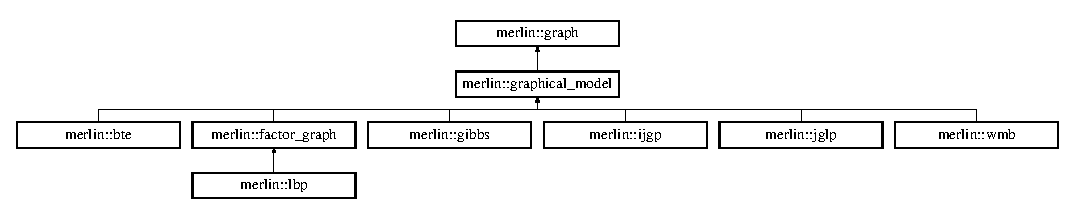
\includegraphics[height=2.440087cm]{classmerlin_1_1graphical__model}
\end{center}
\end{figure}
\subsection*{Public Types}
\begin{DoxyCompactItemize}
\item 
typedef size\+\_\+t \hyperlink{classmerlin_1_1graphical__model_ab2b46f09d8142bb68f243ecadbdabb6b}{findex}\hypertarget{classmerlin_1_1graphical__model_ab2b46f09d8142bb68f243ecadbdabb6b}{}\label{classmerlin_1_1graphical__model_ab2b46f09d8142bb68f243ecadbdabb6b}

\begin{DoxyCompactList}\small\item\em Factor index. \end{DoxyCompactList}\item 
typedef size\+\_\+t \hyperlink{classmerlin_1_1graphical__model_a275006a490bc09239c12a4d93d53b135}{vindex}\hypertarget{classmerlin_1_1graphical__model_a275006a490bc09239c12a4d93d53b135}{}\label{classmerlin_1_1graphical__model_a275006a490bc09239c12a4d93d53b135}

\begin{DoxyCompactList}\small\item\em Variable index. \end{DoxyCompactList}\item 
typedef \hyperlink{classmerlin_1_1set}{set}$<$ \hyperlink{classmerlin_1_1graphical__model_ab2b46f09d8142bb68f243ecadbdabb6b}{findex} $>$ \hyperlink{classmerlin_1_1graphical__model_a615e25ec6594615fddfd4c3c4776b99f}{flist}\hypertarget{classmerlin_1_1graphical__model_a615e25ec6594615fddfd4c3c4776b99f}{}\label{classmerlin_1_1graphical__model_a615e25ec6594615fddfd4c3c4776b99f}

\begin{DoxyCompactList}\small\item\em Collection of factor indices. \end{DoxyCompactList}\end{DoxyCompactItemize}
\subsection*{Public Member Functions}
\begin{DoxyCompactItemize}
\item 
\hyperlink{classmerlin_1_1graphical__model_a5ee627101e4251833f1f6dd40cb34322}{graphical\+\_\+model} ()\hypertarget{classmerlin_1_1graphical__model_a5ee627101e4251833f1f6dd40cb34322}{}\label{classmerlin_1_1graphical__model_a5ee627101e4251833f1f6dd40cb34322}

\begin{DoxyCompactList}\small\item\em Creates an empty graphical model. \end{DoxyCompactList}\item 
\hyperlink{classmerlin_1_1graphical__model_aa35a615de634e3115f0ee3a5fcc7919e}{graphical\+\_\+model} (const \hyperlink{classmerlin_1_1graphical__model}{graphical\+\_\+model} \&gm)
\begin{DoxyCompactList}\small\item\em Creates a graphical model by copying an existing one. \end{DoxyCompactList}\item 
\hyperlink{classmerlin_1_1graphical__model}{graphical\+\_\+model} \& \hyperlink{classmerlin_1_1graphical__model_aa9b0f8a5d4e2098fce8e64f3778245e3}{operator=} (const \hyperlink{classmerlin_1_1graphical__model}{graphical\+\_\+model} \&gm)
\begin{DoxyCompactList}\small\item\em Assignment operator (deep copy). \end{DoxyCompactList}\item 
virtual \hyperlink{classmerlin_1_1graphical__model}{graphical\+\_\+model} $\ast$ \hyperlink{classmerlin_1_1graphical__model_a5315423e0cda62c03beda959b1311f48}{clone} ()
\begin{DoxyCompactList}\small\item\em Clone the graphical model. \end{DoxyCompactList}\item 
\hyperlink{classmerlin_1_1graphical__model_a322196c5146e7c660d5bf1c319fd691a}{graphical\+\_\+model} (std\+::vector$<$ \hyperlink{classmerlin_1_1factor}{factor} $>$ fs)
\begin{DoxyCompactList}\small\item\em Constructor from a list of factors. \end{DoxyCompactList}\item 
{\footnotesize template$<$class Input\+Iterator $>$ }\\\hyperlink{classmerlin_1_1graphical__model_a337d8312dc3d7d8107ea6f7ea6ed435c}{graphical\+\_\+model} (Input\+Iterator first, Input\+Iterator last)
\begin{DoxyCompactList}\small\item\em Creates a graphical model from input iterators. \end{DoxyCompactList}\item 
virtual \hyperlink{classmerlin_1_1graphical__model_a7eed9741a60c050ed1cc0b13602e0a3a}{$\sim$graphical\+\_\+model} ()\hypertarget{classmerlin_1_1graphical__model_a7eed9741a60c050ed1cc0b13602e0a3a}{}\label{classmerlin_1_1graphical__model_a7eed9741a60c050ed1cc0b13602e0a3a}

\begin{DoxyCompactList}\small\item\em Destroys the graphical model. \end{DoxyCompactList}\item 
void \hyperlink{classmerlin_1_1graphical__model_ad67d810e65b40a32f5569d7f82cdfba5}{read} (const char $\ast$file\+\_\+name)
\begin{DoxyCompactList}\small\item\em Read the graphical model from a file in the U\+AI format. \end{DoxyCompactList}\item 
void \hyperlink{classmerlin_1_1graphical__model_a0181edae3b186662262348f4e321e775}{write} (const char $\ast$file\+\_\+name)
\begin{DoxyCompactList}\small\item\em Write the graphical model to a file using the U\+AI format. \end{DoxyCompactList}\item 
bool \hyperlink{classmerlin_1_1graphical__model_aa80358139df9a4e65b659cb04896bc1f}{is\+\_\+markov} ()\hypertarget{classmerlin_1_1graphical__model_aa80358139df9a4e65b659cb04896bc1f}{}\label{classmerlin_1_1graphical__model_aa80358139df9a4e65b659cb04896bc1f}

\begin{DoxyCompactList}\small\item\em Check if graphical model is a Markov or a Bayes net. \end{DoxyCompactList}\item 
std\+::vector$<$ \hyperlink{classmerlin_1_1factor}{factor} $>$ \hyperlink{classmerlin_1_1graphical__model_a6edc6fc8040434b62ab2761805b02525}{assert\+\_\+evidence} (const char $\ast$file\+\_\+name, std\+::map$<$ size\+\_\+t, size\+\_\+t $>$ \&evidence, std\+::map$<$ size\+\_\+t, size\+\_\+t $>$ \&old\+\_\+to\+\_\+new)
\begin{DoxyCompactList}\small\item\em Assert evidence into the graphical model. \end{DoxyCompactList}\item 
std\+::vector$<$ \hyperlink{classmerlin_1_1factor}{factor} $>$ \hyperlink{classmerlin_1_1graphical__model_aa06bf7612a9c5827509504e85760df6e}{assert\+\_\+evidence} (const std\+::map$<$ size\+\_\+t, size\+\_\+t $>$ \&evidence, std\+::map$<$ size\+\_\+t, size\+\_\+t $>$ \&old\+\_\+to\+\_\+new)
\begin{DoxyCompactList}\small\item\em Assert evidence into the graphical model. \end{DoxyCompactList}\item 
size\+\_\+t \hyperlink{classmerlin_1_1graphical__model_af70ee4f7a4414fac4f7568e3c0e5efca}{nvar} () const \hypertarget{classmerlin_1_1graphical__model_af70ee4f7a4414fac4f7568e3c0e5efca}{}\label{classmerlin_1_1graphical__model_af70ee4f7a4414fac4f7568e3c0e5efca}

\begin{DoxyCompactList}\small\item\em Return the number of variables in the model. \end{DoxyCompactList}\item 
\hyperlink{classmerlin_1_1variable}{variable} \hyperlink{classmerlin_1_1graphical__model_a879e8c3766482cc36e96372531e5daef}{var} (\hyperlink{classmerlin_1_1graphical__model_a275006a490bc09239c12a4d93d53b135}{vindex} i) const 
\begin{DoxyCompactList}\small\item\em Convert a variable index to Var object. \end{DoxyCompactList}\item 
size\+\_\+t \hyperlink{classmerlin_1_1graphical__model_ad9cb2599d03e1c60a9201272f461fa5d}{num\+\_\+factors} () const \hypertarget{classmerlin_1_1graphical__model_ad9cb2599d03e1c60a9201272f461fa5d}{}\label{classmerlin_1_1graphical__model_ad9cb2599d03e1c60a9201272f461fa5d}

\begin{DoxyCompactList}\small\item\em Return the number of factors in the model. \end{DoxyCompactList}\item 
const \hyperlink{classmerlin_1_1factor}{factor} \& \hyperlink{classmerlin_1_1graphical__model_ab2c87e3a4cfa3e511e089f3f6b1bd981}{get\+\_\+factor} (\hyperlink{classmerlin_1_1graphical__model_ab2b46f09d8142bb68f243ecadbdabb6b}{findex} idx) const 
\begin{DoxyCompactList}\small\item\em Accessor for a factor. \end{DoxyCompactList}\item 
const std\+::vector$<$ \hyperlink{classmerlin_1_1factor}{factor} $>$ \& \hyperlink{classmerlin_1_1graphical__model_a0d80510846922ce3cabf088aa04af040}{get\+\_\+factors} () const 
\begin{DoxyCompactList}\small\item\em Accessor for the factor container. \end{DoxyCompactList}\item 
const \hyperlink{classmerlin_1_1graphical__model_a615e25ec6594615fddfd4c3c4776b99f}{flist} \& \hyperlink{classmerlin_1_1graphical__model_a2e00ea842135f7a2169278ce19cda9d9}{with\+\_\+variable} (const \hyperlink{classmerlin_1_1variable}{variable} \&v) const 
\begin{DoxyCompactList}\small\item\em Factors depending on a variable. \end{DoxyCompactList}\item 
\hyperlink{classmerlin_1_1graphical__model_a615e25ec6594615fddfd4c3c4776b99f}{flist} \hyperlink{classmerlin_1_1graphical__model_a24454dad4b1754b5c58a7fa3b2738739}{with\+\_\+variable\+\_\+set} (const \hyperlink{classmerlin_1_1variable__set}{variable\+\_\+set} \&vs) const 
\begin{DoxyCompactList}\small\item\em Union of factors depending on a set of variables. \end{DoxyCompactList}\item 
\hyperlink{classmerlin_1_1graphical__model_a615e25ec6594615fddfd4c3c4776b99f}{flist} \hyperlink{classmerlin_1_1graphical__model_ac2841d98a5d54bc5bf384facb939e57a}{intersects} (const \hyperlink{classmerlin_1_1variable__set}{variable\+\_\+set} \&vs) const 
\begin{DoxyCompactList}\small\item\em Intersection of factors depending on a set of variables. \end{DoxyCompactList}\item 
\hyperlink{classmerlin_1_1graphical__model_a615e25ec6594615fddfd4c3c4776b99f}{flist} \hyperlink{classmerlin_1_1graphical__model_ad2febd01b65cab5c41a85ed2850a58dd}{contains} (const \hyperlink{classmerlin_1_1variable}{variable} \&v) const 
\begin{DoxyCompactList}\small\item\em Factors depending on a variable. \end{DoxyCompactList}\item 
\hyperlink{classmerlin_1_1graphical__model_a615e25ec6594615fddfd4c3c4776b99f}{flist} \hyperlink{classmerlin_1_1graphical__model_aafb1db01ca3f08e67bfc0bf0a01e9214}{contains} (const \hyperlink{classmerlin_1_1variable__set}{variable\+\_\+set} \&vs) const 
\begin{DoxyCompactList}\small\item\em Union of factors depending on a set of variables. \end{DoxyCompactList}\item 
\hyperlink{classmerlin_1_1graphical__model_a615e25ec6594615fddfd4c3c4776b99f}{flist} \hyperlink{classmerlin_1_1graphical__model_a399c5636919586bdaeeda03707ed9ba6}{contained\+\_\+by} (const \hyperlink{classmerlin_1_1variable__set}{variable\+\_\+set} \&vs) const 
\begin{DoxyCompactList}\small\item\em Factors contained by a set of variables. \end{DoxyCompactList}\item 
\hyperlink{classmerlin_1_1variable__set}{variable\+\_\+set} \hyperlink{classmerlin_1_1graphical__model_abedcfa3faf1b0c76465f44a24de37e75}{markov\+\_\+blanket} (const \hyperlink{classmerlin_1_1variable}{variable} \&v) const 
\begin{DoxyCompactList}\small\item\em Markov blanket of a variable. \end{DoxyCompactList}\item 
\hyperlink{classmerlin_1_1variable__set}{variable\+\_\+set} \hyperlink{classmerlin_1_1graphical__model_af6b2d0ec1085f9318dec785c3d47e3a3}{markov\+\_\+blanket} (const \hyperlink{classmerlin_1_1variable__set}{variable\+\_\+set} \&vs) const 
\begin{DoxyCompactList}\small\item\em Markov blanket of a set of variables. \end{DoxyCompactList}\item 
std\+::vector$<$ \hyperlink{classmerlin_1_1variable__set}{variable\+\_\+set} $>$ \hyperlink{classmerlin_1_1graphical__model_ac27c6c49cb3f55fa248c0a4adba2cb92}{mrf} () const 
\begin{DoxyCompactList}\small\item\em Full adjacency matrix. \end{DoxyCompactList}\item 
virtual \hyperlink{classmerlin_1_1graphical__model_ab2b46f09d8142bb68f243ecadbdabb6b}{findex} \hyperlink{classmerlin_1_1graphical__model_a7edaca0ce3ddea09f64e6bab406bfab8}{add\+\_\+factor} (const \hyperlink{classmerlin_1_1factor}{factor} \&F)
\begin{DoxyCompactList}\small\item\em Add a new factor to the model. \end{DoxyCompactList}\item 
virtual void \hyperlink{classmerlin_1_1graphical__model_aabcdb025068a429bc1ab8d62e38065d9}{remove\+\_\+factor} (\hyperlink{classmerlin_1_1graphical__model_ab2b46f09d8142bb68f243ecadbdabb6b}{findex} idx)
\begin{DoxyCompactList}\small\item\em Remove a factor from the model. \end{DoxyCompactList}\item 
void \hyperlink{classmerlin_1_1graphical__model_a01c2f86dfbe20a3f0c8b4b057c9ef61a}{clear\+\_\+factors} ()\hypertarget{classmerlin_1_1graphical__model_a01c2f86dfbe20a3f0c8b4b057c9ef61a}{}\label{classmerlin_1_1graphical__model_a01c2f86dfbe20a3f0c8b4b057c9ef61a}

\begin{DoxyCompactList}\small\item\em Remove all factors. \end{DoxyCompactList}\item 
\hyperlink{classmerlin_1_1graphical__model_ab2b46f09d8142bb68f243ecadbdabb6b}{findex} \hyperlink{classmerlin_1_1graphical__model_a87052337ee867285fc2700d00995cc1e}{smallest} (const \hyperlink{classmerlin_1_1graphical__model_a615e25ec6594615fddfd4c3c4776b99f}{flist} \&fl)
\begin{DoxyCompactList}\small\item\em Find the factor with the smallest scope. \end{DoxyCompactList}\item 
\hyperlink{classmerlin_1_1graphical__model_ab2b46f09d8142bb68f243ecadbdabb6b}{findex} \hyperlink{classmerlin_1_1graphical__model_abe468de8ee79157ccfd329dae24fa221}{largest} (const \hyperlink{classmerlin_1_1graphical__model_a615e25ec6594615fddfd4c3c4776b99f}{flist} \&fl)
\begin{DoxyCompactList}\small\item\em Find the factor with the largest scope. \end{DoxyCompactList}\item 
bool \hyperlink{classmerlin_1_1graphical__model_ab898aaf86745e1a842aa9784cd91f86c}{is\+\_\+binary} () const 
\begin{DoxyCompactList}\small\item\em Check if a binary model. \end{DoxyCompactList}\item 
bool \hyperlink{classmerlin_1_1graphical__model_ace118985e3679cdacfc5332947dfb444}{is\+\_\+pairwise} () const 
\begin{DoxyCompactList}\small\item\em Check if a pairwise model. \end{DoxyCompactList}\item 
\hyperlink{classmerlin_1_1factor}{factor} \hyperlink{classmerlin_1_1graphical__model_a7b3e5d2e0b423e481019f224971e0d29}{joint} (size\+\_\+t maxsize=0) const 
\begin{DoxyCompactList}\small\item\em Directly calculate joint distribution function. \end{DoxyCompactList}\item 
size\+\_\+t \hyperlink{classmerlin_1_1graphical__model_a109e5f71e08368d3460ab4a74e1074fb}{induced\+\_\+width} (const variable\+\_\+order\+\_\+t \&\hyperlink{classmerlin_1_1graphical__model_a90bcf3fb02f0f43bf57520e834875c78}{order}) const 
\begin{DoxyCompactList}\small\item\em Find the induced width (complexity) of an elimination order. \end{DoxyCompactList}\item 
std\+::pair$<$ size\+\_\+t, size\+\_\+t $>$ \hyperlink{classmerlin_1_1graphical__model_a60914b4dfd137288d059280a29db1d3f}{pseudo\+\_\+tree\+\_\+size} (const variable\+\_\+order\+\_\+t \&\hyperlink{classmerlin_1_1graphical__model_a90bcf3fb02f0f43bf57520e834875c78}{order}) const 
\begin{DoxyCompactList}\small\item\em Find induced width and pseudo tree height of an elimination order. \end{DoxyCompactList}\item 
std\+::vector$<$ \hyperlink{classmerlin_1_1graphical__model_a275006a490bc09239c12a4d93d53b135}{vindex} $>$ \hyperlink{classmerlin_1_1graphical__model_ab939be0ea59b1bb676e4b4ea5de0d625}{pseudo\+\_\+tree} (const variable\+\_\+order\+\_\+t \&\hyperlink{classmerlin_1_1graphical__model_a90bcf3fb02f0f43bf57520e834875c78}{order}) const 
\begin{DoxyCompactList}\small\item\em Find the pseudo tree corresponding to an elimination order. \end{DoxyCompactList}\item 
\hyperlink{classmerlin_1_1graphical__model_a912837b886d835280f269f1845dcb752}{M\+E\+R\+\_\+\+E\+N\+UM} (Order\+Method, Min\+Fill, Wt\+Min\+Fill, Min\+Width, Wt\+Min\+Width, Random)\hypertarget{classmerlin_1_1graphical__model_a912837b886d835280f269f1845dcb752}{}\label{classmerlin_1_1graphical__model_a912837b886d835280f269f1845dcb752}

\begin{DoxyCompactList}\small\item\em Variable ordering methods. \end{DoxyCompactList}\item 
variable\+\_\+order\+\_\+t \hyperlink{classmerlin_1_1graphical__model_a90bcf3fb02f0f43bf57520e834875c78}{order} (Order\+Method ord\+\_\+type) const 
\begin{DoxyCompactList}\small\item\em Find a variable elimination order. \end{DoxyCompactList}\item 
variable\+\_\+order\+\_\+t \hyperlink{classmerlin_1_1graphical__model_aaed0e52114f9dc66f14126280cf6b68e}{order2} (Order\+Method ord\+\_\+type) const 
\begin{DoxyCompactList}\small\item\em Find a variable elimination order. \end{DoxyCompactList}\item 
variable\+\_\+order\+\_\+t \hyperlink{classmerlin_1_1graphical__model_a46a0f34fa6a0d021a2ae3161da271feb}{order2} (Order\+Method ord\+\_\+type, std\+::vector$<$ bool $>$ var\+\_\+types) const 
\begin{DoxyCompactList}\small\item\em Find a constrained variable elimination order. \end{DoxyCompactList}\item 
variable\+\_\+order\+\_\+t \hyperlink{classmerlin_1_1graphical__model_a8a722099188b11d7e44b668c13e836f2}{order} (Order\+Method ord\+\_\+type, std\+::vector$<$ bool $>$ var\+\_\+types) const 
\begin{DoxyCompactList}\small\item\em Find a constrained variable elimination order. \end{DoxyCompactList}\item 
void \hyperlink{classmerlin_1_1graphical__model_a42f9b6f295100feefaaec09cef03c173}{improve\+\_\+order} (Order\+Method ord\+\_\+type, double \&old\+\_\+score, variable\+\_\+order\+\_\+t \&old\+\_\+order) const 
\begin{DoxyCompactList}\small\item\em Look for a better order iteratively. \end{DoxyCompactList}\item 
void \hyperlink{classmerlin_1_1graphical__model_aa953b05dcb91b18c8726324bcbe7eb24}{insert} (std\+::vector$<$ \hyperlink{classmerlin_1_1graphical__model_a615e25ec6594615fddfd4c3c4776b99f}{flist} $>$ \&adj, \hyperlink{classmerlin_1_1graphical__model_ab2b46f09d8142bb68f243ecadbdabb6b}{findex} idx, const \hyperlink{classmerlin_1_1variable__set}{variable\+\_\+set} \&vs)
\begin{DoxyCompactList}\small\item\em Add the scope of a factor to the adjacency list. \end{DoxyCompactList}\item 
void \hyperlink{classmerlin_1_1graphical__model_add6a62d0d4a2091944bf18ad108ff1ba}{erase} (std\+::vector$<$ \hyperlink{classmerlin_1_1graphical__model_a615e25ec6594615fddfd4c3c4776b99f}{flist} $>$ \&adj, \hyperlink{classmerlin_1_1graphical__model_ab2b46f09d8142bb68f243ecadbdabb6b}{findex} idx, const \hyperlink{classmerlin_1_1variable__set}{variable\+\_\+set} \&vs)
\begin{DoxyCompactList}\small\item\em Remove the scope of a factor from the adjacency list. \end{DoxyCompactList}\item 
std\+::vector$<$ size\+\_\+t $>$ \hyperlink{classmerlin_1_1graphical__model_ad1d7f268d7beb504a1e6ed79a1fca676}{max\+\_\+simple} ()\hypertarget{classmerlin_1_1graphical__model_ad1d7f268d7beb504a1e6ed79a1fca676}{}\label{classmerlin_1_1graphical__model_ad1d7f268d7beb504a1e6ed79a1fca676}

\begin{DoxyCompactList}\small\item\em Find smallest factor with each variable and select its optimum. \end{DoxyCompactList}\item 
std\+::vector$<$ size\+\_\+t $>$ \hyperlink{classmerlin_1_1graphical__model_a29f7fb295dea0c444de5fe03f1da1e91}{max\+\_\+sequential} (const variable\+\_\+order\+\_\+t \&\hyperlink{classmerlin_1_1graphical__model_a90bcf3fb02f0f43bf57520e834875c78}{order})\hypertarget{classmerlin_1_1graphical__model_a29f7fb295dea0c444de5fe03f1da1e91}{}\label{classmerlin_1_1graphical__model_a29f7fb295dea0c444de5fe03f1da1e91}

\begin{DoxyCompactList}\small\item\em Find {\itshape maxmarginal} for variable and select optimum given those so far. \end{DoxyCompactList}\item 
double \hyperlink{classmerlin_1_1graphical__model_aaf48222f85e0d6cbf1b289219953863f}{logP} (const std\+::vector$<$ size\+\_\+t $>$ \&config)\hypertarget{classmerlin_1_1graphical__model_aaf48222f85e0d6cbf1b289219953863f}{}\label{classmerlin_1_1graphical__model_aaf48222f85e0d6cbf1b289219953863f}

\begin{DoxyCompactList}\small\item\em Compute the log-\/probability of a particular (complete) configuration. \end{DoxyCompactList}\item 
double \hyperlink{classmerlin_1_1graphical__model_afad10d82af1bf8a138e00a58f98ec18c}{get\+\_\+global\+\_\+const} () const \hypertarget{classmerlin_1_1graphical__model_afad10d82af1bf8a138e00a58f98ec18c}{}\label{classmerlin_1_1graphical__model_afad10d82af1bf8a138e00a58f98ec18c}

\begin{DoxyCompactList}\small\item\em Return the constant resulted from asserting evidence in the model. \end{DoxyCompactList}\end{DoxyCompactItemize}
\subsection*{Protected Member Functions}
\begin{DoxyCompactItemize}
\item 
size\+\_\+t \hyperlink{classmerlin_1_1graphical__model_a643284acb0bff3c9b6d0aed42e06ee0e}{\+\_\+vindex} (const \hyperlink{classmerlin_1_1variable}{variable} \&v) const 
\begin{DoxyCompactList}\small\item\em Look up the index of a variable. \end{DoxyCompactList}\item 
\hyperlink{classmerlin_1_1graphical__model_a615e25ec6594615fddfd4c3c4776b99f}{flist} \& \hyperlink{classmerlin_1_1graphical__model_afe30032fede9c900ded128a6e95b33fb}{\+\_\+with\+\_\+variable} (const \hyperlink{classmerlin_1_1variable}{variable} \&v)
\begin{DoxyCompactList}\small\item\em Mutable accessor of adjacency. \end{DoxyCompactList}\item 
void \hyperlink{classmerlin_1_1graphical__model_a072ca3f28708cb4bab36db5b638ce861}{fixup} ()\hypertarget{classmerlin_1_1graphical__model_a072ca3f28708cb4bab36db5b638ce861}{}\label{classmerlin_1_1graphical__model_a072ca3f28708cb4bab36db5b638ce861}

\begin{DoxyCompactList}\small\item\em Internal function for ensuring consistency of the model. \end{DoxyCompactList}\item 
double \hyperlink{classmerlin_1_1graphical__model_a4bc13ae4aa3bdba76bf398bfe07308ca}{order\+\_\+score} (const std\+::vector$<$ \hyperlink{classmerlin_1_1variable__set}{variable\+\_\+set} $>$ \&adj, size\+\_\+t i, Order\+Method k\+O\+Type) const 
\begin{DoxyCompactList}\small\item\em Compute the score of a variable for the elimination order. \end{DoxyCompactList}\item 
variable\+\_\+order\+\_\+t \hyperlink{classmerlin_1_1graphical__model_aae2a2d690804361f0edc4ca1147dcf39}{order\+\_\+random} () const \hypertarget{classmerlin_1_1graphical__model_aae2a2d690804361f0edc4ca1147dcf39}{}\label{classmerlin_1_1graphical__model_aae2a2d690804361f0edc4ca1147dcf39}

\begin{DoxyCompactList}\small\item\em Create a random elimination order. \end{DoxyCompactList}\end{DoxyCompactItemize}
\subsection*{Protected Attributes}
\begin{DoxyCompactItemize}
\item 
std\+::vector$<$ \hyperlink{classmerlin_1_1factor}{factor} $>$ \hyperlink{classmerlin_1_1graphical__model_aecae0801175e5752efc53146f9c7030e}{m\+\_\+factors}\hypertarget{classmerlin_1_1graphical__model_aecae0801175e5752efc53146f9c7030e}{}\label{classmerlin_1_1graphical__model_aecae0801175e5752efc53146f9c7030e}

\begin{DoxyCompactList}\small\item\em Collection of all factors in the model. \end{DoxyCompactList}\item 
bool \hyperlink{classmerlin_1_1graphical__model_a0f18dee551857422661f91927f9dda52}{m\+\_\+markov}\hypertarget{classmerlin_1_1graphical__model_a0f18dee551857422661f91927f9dda52}{}\label{classmerlin_1_1graphical__model_a0f18dee551857422661f91927f9dda52}

\begin{DoxyCompactList}\small\item\em Markov or Bayes network. Default is true (Markov) \end{DoxyCompactList}\end{DoxyCompactItemize}
\subsection*{Friends}
\begin{DoxyCompactItemize}
\item 
std\+::ostream \& \hyperlink{classmerlin_1_1graphical__model_ab797c308605a6f3098645515dfe2ddc0}{operator$<$$<$} (std\+::ostream \&out, const \hyperlink{classmerlin_1_1graphical__model}{graphical\+\_\+model} \&gm)
\begin{DoxyCompactList}\small\item\em Output operator. \end{DoxyCompactList}\end{DoxyCompactItemize}
\subsection*{Additional Inherited Members}


\subsection{Detailed Description}
Graphical model base class. 

Simplest form of a {\itshape graphical model}, namely just a collection of variables and factors (defined on subsets of variables). Internally, factors and variables are mainly referenced by integer indices, with 0 $<$= f $<$ n\+Factors() and 0 $<$= v $<$ \hyperlink{classmerlin_1_1graphical__model_af70ee4f7a4414fac4f7568e3c0e5efca}{nvar()}. However, many interface functions are called using a variable object, Var(label,dim). To convert, var(v) gives the vth Var object and the internal function \+\_\+vindex(\+V) gives the index corresponding to variable object V. 

Definition at line 47 of file graphical\+\_\+model.\+h.



\subsection{Constructor \& Destructor Documentation}
\index{merlin\+::graphical\+\_\+model@{merlin\+::graphical\+\_\+model}!graphical\+\_\+model@{graphical\+\_\+model}}
\index{graphical\+\_\+model@{graphical\+\_\+model}!merlin\+::graphical\+\_\+model@{merlin\+::graphical\+\_\+model}}
\subsubsection[{\texorpdfstring{graphical\+\_\+model(const graphical\+\_\+model \&gm)}{graphical_model(const graphical_model &gm)}}]{\setlength{\rightskip}{0pt plus 5cm}merlin\+::graphical\+\_\+model\+::graphical\+\_\+model (
\begin{DoxyParamCaption}
\item[{const {\bf graphical\+\_\+model} \&}]{gm}
\end{DoxyParamCaption}
)\hspace{0.3cm}{\ttfamily [inline]}}\hypertarget{classmerlin_1_1graphical__model_aa35a615de634e3115f0ee3a5fcc7919e}{}\label{classmerlin_1_1graphical__model_aa35a615de634e3115f0ee3a5fcc7919e}


Creates a graphical model by copying an existing one. 


\begin{DoxyParams}{Parameters}
{\em gm} & An object of the same type \\
\hline
\end{DoxyParams}


Definition at line 69 of file graphical\+\_\+model.\+h.

\index{merlin\+::graphical\+\_\+model@{merlin\+::graphical\+\_\+model}!graphical\+\_\+model@{graphical\+\_\+model}}
\index{graphical\+\_\+model@{graphical\+\_\+model}!merlin\+::graphical\+\_\+model@{merlin\+::graphical\+\_\+model}}
\subsubsection[{\texorpdfstring{graphical\+\_\+model(std\+::vector$<$ factor $>$ fs)}{graphical_model(std::vector< factor > fs)}}]{\setlength{\rightskip}{0pt plus 5cm}merlin\+::graphical\+\_\+model\+::graphical\+\_\+model (
\begin{DoxyParamCaption}
\item[{std\+::vector$<$ {\bf factor} $>$}]{fs}
\end{DoxyParamCaption}
)\hspace{0.3cm}{\ttfamily [inline]}}\hypertarget{classmerlin_1_1graphical__model_a322196c5146e7c660d5bf1c319fd691a}{}\label{classmerlin_1_1graphical__model_a322196c5146e7c660d5bf1c319fd691a}


Constructor from a list of factors. 


\begin{DoxyParams}{Parameters}
{\em fs} & The list of factors \\
\hline
\end{DoxyParams}


Definition at line 102 of file graphical\+\_\+model.\+h.



References fixup().

\index{merlin\+::graphical\+\_\+model@{merlin\+::graphical\+\_\+model}!graphical\+\_\+model@{graphical\+\_\+model}}
\index{graphical\+\_\+model@{graphical\+\_\+model}!merlin\+::graphical\+\_\+model@{merlin\+::graphical\+\_\+model}}
\subsubsection[{\texorpdfstring{graphical\+\_\+model(\+Input\+Iterator first, Input\+Iterator last)}{graphical_model(InputIterator first, InputIterator last)}}]{\setlength{\rightskip}{0pt plus 5cm}template$<$class Input\+Iterator $>$ merlin\+::graphical\+\_\+model\+::graphical\+\_\+model (
\begin{DoxyParamCaption}
\item[{Input\+Iterator}]{first, }
\item[{Input\+Iterator}]{last}
\end{DoxyParamCaption}
)\hspace{0.3cm}{\ttfamily [inline]}}\hypertarget{classmerlin_1_1graphical__model_a337d8312dc3d7d8107ea6f7ea6ed435c}{}\label{classmerlin_1_1graphical__model_a337d8312dc3d7d8107ea6f7ea6ed435c}


Creates a graphical model from input iterators. 


\begin{DoxyParams}{Parameters}
{\em first} & The iterator to beginning \\
\hline
{\em last} & The iterator to end \\
\hline
\end{DoxyParams}


Definition at line 113 of file graphical\+\_\+model.\+h.



References fixup().



\subsection{Member Function Documentation}
\index{merlin\+::graphical\+\_\+model@{merlin\+::graphical\+\_\+model}!\+\_\+vindex@{\+\_\+vindex}}
\index{\+\_\+vindex@{\+\_\+vindex}!merlin\+::graphical\+\_\+model@{merlin\+::graphical\+\_\+model}}
\subsubsection[{\texorpdfstring{\+\_\+vindex(const variable \&v) const }{_vindex(const variable &v) const }}]{\setlength{\rightskip}{0pt plus 5cm}size\+\_\+t merlin\+::graphical\+\_\+model\+::\+\_\+vindex (
\begin{DoxyParamCaption}
\item[{const {\bf variable} \&}]{v}
\end{DoxyParamCaption}
) const\hspace{0.3cm}{\ttfamily [inline]}, {\ttfamily [protected]}}\hypertarget{classmerlin_1_1graphical__model_a643284acb0bff3c9b6d0aed42e06ee0e}{}\label{classmerlin_1_1graphical__model_a643284acb0bff3c9b6d0aed42e06ee0e}


Look up the index of a variable. 


\begin{DoxyParams}{Parameters}
{\em v} & The variable object \\
\hline
\end{DoxyParams}
\begin{DoxyReturn}{Returns}
the index corresponding to the variable in the model. 
\end{DoxyReturn}


Definition at line 1441 of file graphical\+\_\+model.\+h.



References merlin\+::variable\+::label().



Referenced by \+\_\+with\+\_\+variable(), add\+\_\+factor(), merlin\+::factor\+\_\+graph\+::create\+\_\+factor\+\_\+graph(), fixup(), improve\+\_\+order(), induced\+\_\+width(), merlin\+::factor\+\_\+graph\+::local\+\_\+factor(), order(), order2(), order\+\_\+score(), pseudo\+\_\+tree(), pseudo\+\_\+tree\+\_\+size(), merlin\+::factor\+\_\+graph\+::remove\+\_\+factor(), merlin\+::factor\+\_\+graph\+::span\+\_\+tree(), and with\+\_\+variable().

\index{merlin\+::graphical\+\_\+model@{merlin\+::graphical\+\_\+model}!\+\_\+with\+\_\+variable@{\+\_\+with\+\_\+variable}}
\index{\+\_\+with\+\_\+variable@{\+\_\+with\+\_\+variable}!merlin\+::graphical\+\_\+model@{merlin\+::graphical\+\_\+model}}
\subsubsection[{\texorpdfstring{\+\_\+with\+\_\+variable(const variable \&v)}{_with_variable(const variable &v)}}]{\setlength{\rightskip}{0pt plus 5cm}{\bf flist}\& merlin\+::graphical\+\_\+model\+::\+\_\+with\+\_\+variable (
\begin{DoxyParamCaption}
\item[{const {\bf variable} \&}]{v}
\end{DoxyParamCaption}
)\hspace{0.3cm}{\ttfamily [inline]}, {\ttfamily [protected]}}\hypertarget{classmerlin_1_1graphical__model_afe30032fede9c900ded128a6e95b33fb}{}\label{classmerlin_1_1graphical__model_afe30032fede9c900ded128a6e95b33fb}


Mutable accessor of adjacency. 


\begin{DoxyParams}{Parameters}
{\em v} & The variable object \\
\hline
\end{DoxyParams}
\begin{DoxyReturn}{Returns}
the list of factors containing the variable in their scope. 
\end{DoxyReturn}


Definition at line 1450 of file graphical\+\_\+model.\+h.



References \+\_\+vindex().



Referenced by fixup().

\index{merlin\+::graphical\+\_\+model@{merlin\+::graphical\+\_\+model}!add\+\_\+factor@{add\+\_\+factor}}
\index{add\+\_\+factor@{add\+\_\+factor}!merlin\+::graphical\+\_\+model@{merlin\+::graphical\+\_\+model}}
\subsubsection[{\texorpdfstring{add\+\_\+factor(const factor \&\+F)}{add_factor(const factor &F)}}]{\setlength{\rightskip}{0pt plus 5cm}virtual {\bf findex} merlin\+::graphical\+\_\+model\+::add\+\_\+factor (
\begin{DoxyParamCaption}
\item[{const {\bf factor} \&}]{F}
\end{DoxyParamCaption}
)\hspace{0.3cm}{\ttfamily [inline]}, {\ttfamily [virtual]}}\hypertarget{classmerlin_1_1graphical__model_a7edaca0ce3ddea09f64e6bab406bfab8}{}\label{classmerlin_1_1graphical__model_a7edaca0ce3ddea09f64e6bab406bfab8}


Add a new factor to the model. 


\begin{DoxyParams}{Parameters}
{\em F} & The factor to be added \\
\hline
\end{DoxyParams}
\begin{DoxyReturn}{Returns}
the index associated with the newly added factor. 
\end{DoxyReturn}


Reimplemented in \hyperlink{classmerlin_1_1factor__graph_a5899fc5d235ad8681c1437e2845f798d}{merlin\+::factor\+\_\+graph}.



Definition at line 562 of file graphical\+\_\+model.\+h.



References \+\_\+vindex(), merlin\+::graph\+::add\+\_\+node(), merlin\+::variable\+\_\+set\+::begin(), merlin\+::variable\+\_\+set\+::end(), insert(), m\+\_\+factors, num\+\_\+factors(), and merlin\+::factor\+::vars().



Referenced by merlin\+::factor\+\_\+graph\+::add\+\_\+factor(), merlin\+::factor\+\_\+graph\+::create\+\_\+factor\+\_\+graph(), merlin\+::bte\+::init(), merlin\+::ijgp\+::init(), merlin\+::wmb\+::init(), and merlin\+::jglp\+::run().

\index{merlin\+::graphical\+\_\+model@{merlin\+::graphical\+\_\+model}!assert\+\_\+evidence@{assert\+\_\+evidence}}
\index{assert\+\_\+evidence@{assert\+\_\+evidence}!merlin\+::graphical\+\_\+model@{merlin\+::graphical\+\_\+model}}
\subsubsection[{\texorpdfstring{assert\+\_\+evidence(const char $\ast$file\+\_\+name, std\+::map$<$ size\+\_\+t, size\+\_\+t $>$ \&evidence, std\+::map$<$ size\+\_\+t, size\+\_\+t $>$ \&old\+\_\+to\+\_\+new)}{assert_evidence(const char *file_name, std::map< size_t, size_t > &evidence, std::map< size_t, size_t > &old_to_new)}}]{\setlength{\rightskip}{0pt plus 5cm}std\+::vector$<${\bf factor}$>$ merlin\+::graphical\+\_\+model\+::assert\+\_\+evidence (
\begin{DoxyParamCaption}
\item[{const char $\ast$}]{file\+\_\+name, }
\item[{std\+::map$<$ size\+\_\+t, size\+\_\+t $>$ \&}]{evidence, }
\item[{std\+::map$<$ size\+\_\+t, size\+\_\+t $>$ \&}]{old\+\_\+to\+\_\+new}
\end{DoxyParamCaption}
)\hspace{0.3cm}{\ttfamily [inline]}}\hypertarget{classmerlin_1_1graphical__model_a6edc6fc8040434b62ab2761805b02525}{}\label{classmerlin_1_1graphical__model_a6edc6fc8040434b62ab2761805b02525}


Assert evidence into the graphical model. 


\begin{DoxyParams}[1]{Parameters}
\mbox{\tt in}  & {\em file\+\_\+name} & The full path to a file containing the evidence \\
\hline
\mbox{\tt out}  & {\em evidence} & The map containing evidence variable value pairs \\
\hline
\mbox{\tt out}  & {\em old\+\_\+to\+\_\+new} & The mappings between old and new variable indexes \\
\hline
\end{DoxyParams}
\begin{DoxyReturn}{Returns}
the list of new factors resulting from conditioning on the evidence. 
\end{DoxyReturn}


Definition at line 272 of file graphical\+\_\+model.\+h.



References merlin\+::variable\+\_\+set\+::begin(), merlin\+::factor\+::condition(), merlin\+::variable\+\_\+set\+::contains(), merlin\+::variable\+\_\+set\+::end(), merlin\+::factor\+::isscalar(), m\+\_\+factors, merlin\+::factor\+::table(), var(), and merlin\+::factor\+::vars().



Referenced by Merlin\+::run().

\index{merlin\+::graphical\+\_\+model@{merlin\+::graphical\+\_\+model}!assert\+\_\+evidence@{assert\+\_\+evidence}}
\index{assert\+\_\+evidence@{assert\+\_\+evidence}!merlin\+::graphical\+\_\+model@{merlin\+::graphical\+\_\+model}}
\subsubsection[{\texorpdfstring{assert\+\_\+evidence(const std\+::map$<$ size\+\_\+t, size\+\_\+t $>$ \&evidence, std\+::map$<$ size\+\_\+t, size\+\_\+t $>$ \&old\+\_\+to\+\_\+new)}{assert_evidence(const std::map< size_t, size_t > &evidence, std::map< size_t, size_t > &old_to_new)}}]{\setlength{\rightskip}{0pt plus 5cm}std\+::vector$<${\bf factor}$>$ merlin\+::graphical\+\_\+model\+::assert\+\_\+evidence (
\begin{DoxyParamCaption}
\item[{const std\+::map$<$ size\+\_\+t, size\+\_\+t $>$ \&}]{evidence, }
\item[{std\+::map$<$ size\+\_\+t, size\+\_\+t $>$ \&}]{old\+\_\+to\+\_\+new}
\end{DoxyParamCaption}
)\hspace{0.3cm}{\ttfamily [inline]}}\hypertarget{classmerlin_1_1graphical__model_aa06bf7612a9c5827509504e85760df6e}{}\label{classmerlin_1_1graphical__model_aa06bf7612a9c5827509504e85760df6e}


Assert evidence into the graphical model. 


\begin{DoxyParams}[1]{Parameters}
\mbox{\tt in}  & {\em evidence} & The map containing evidence variable value pairs \\
\hline
\mbox{\tt out}  & {\em old\+\_\+to\+\_\+new} & The mappings between old and new variable indexes \\
\hline
\end{DoxyParams}
\begin{DoxyReturn}{Returns}
the list of new factors resulting from conditioning on the evidence. 
\end{DoxyReturn}


Definition at line 345 of file graphical\+\_\+model.\+h.



References merlin\+::variable\+\_\+set\+::begin(), merlin\+::factor\+::condition(), merlin\+::variable\+\_\+set\+::contains(), merlin\+::variable\+\_\+set\+::end(), merlin\+::factor\+::isscalar(), m\+\_\+factors, merlin\+::variable\+::states(), merlin\+::factor\+::table(), var(), and merlin\+::factor\+::vars().

\index{merlin\+::graphical\+\_\+model@{merlin\+::graphical\+\_\+model}!clone@{clone}}
\index{clone@{clone}!merlin\+::graphical\+\_\+model@{merlin\+::graphical\+\_\+model}}
\subsubsection[{\texorpdfstring{clone()}{clone()}}]{\setlength{\rightskip}{0pt plus 5cm}virtual {\bf graphical\+\_\+model}$\ast$ merlin\+::graphical\+\_\+model\+::clone (
\begin{DoxyParamCaption}
{}
\end{DoxyParamCaption}
)\hspace{0.3cm}{\ttfamily [inline]}, {\ttfamily [virtual]}}\hypertarget{classmerlin_1_1graphical__model_a5315423e0cda62c03beda959b1311f48}{}\label{classmerlin_1_1graphical__model_a5315423e0cda62c03beda959b1311f48}


Clone the graphical model. 

\begin{DoxyReturn}{Returns}
the pointer to the new object representing the copy of the current model. 
\end{DoxyReturn}


Reimplemented in \hyperlink{classmerlin_1_1factor__graph_a485d9039df843d2db668782ac9c90c8a}{merlin\+::factor\+\_\+graph}.



Definition at line 93 of file graphical\+\_\+model.\+h.



References graphical\+\_\+model().



Referenced by Merlin\+::read\+\_\+model().

\index{merlin\+::graphical\+\_\+model@{merlin\+::graphical\+\_\+model}!contained\+\_\+by@{contained\+\_\+by}}
\index{contained\+\_\+by@{contained\+\_\+by}!merlin\+::graphical\+\_\+model@{merlin\+::graphical\+\_\+model}}
\subsubsection[{\texorpdfstring{contained\+\_\+by(const variable\+\_\+set \&vs) const }{contained_by(const variable_set &vs) const }}]{\setlength{\rightskip}{0pt plus 5cm}{\bf flist} merlin\+::graphical\+\_\+model\+::contained\+\_\+by (
\begin{DoxyParamCaption}
\item[{const {\bf variable\+\_\+set} \&}]{vs}
\end{DoxyParamCaption}
) const\hspace{0.3cm}{\ttfamily [inline]}}\hypertarget{classmerlin_1_1graphical__model_a399c5636919586bdaeeda03707ed9ba6}{}\label{classmerlin_1_1graphical__model_a399c5636919586bdaeeda03707ed9ba6}


Factors contained by a set of variables. 


\begin{DoxyParams}{Parameters}
{\em vs} & The set of variables \\
\hline
\end{DoxyParams}
\begin{DoxyReturn}{Returns}
the list of factor indexes contained by the set of variables. 
\end{DoxyReturn}


Definition at line 508 of file graphical\+\_\+model.\+h.



References intersects(), m\+\_\+factors, and merlin\+::set$<$ T $>$\+::size().

\index{merlin\+::graphical\+\_\+model@{merlin\+::graphical\+\_\+model}!contains@{contains}}
\index{contains@{contains}!merlin\+::graphical\+\_\+model@{merlin\+::graphical\+\_\+model}}
\subsubsection[{\texorpdfstring{contains(const variable \&v) const }{contains(const variable &v) const }}]{\setlength{\rightskip}{0pt plus 5cm}{\bf flist} merlin\+::graphical\+\_\+model\+::contains (
\begin{DoxyParamCaption}
\item[{const {\bf variable} \&}]{v}
\end{DoxyParamCaption}
) const\hspace{0.3cm}{\ttfamily [inline]}}\hypertarget{classmerlin_1_1graphical__model_ad2febd01b65cab5c41a85ed2850a58dd}{}\label{classmerlin_1_1graphical__model_ad2febd01b65cab5c41a85ed2850a58dd}


Factors depending on a variable. 


\begin{DoxyParams}{Parameters}
{\em v} & The variable object \\
\hline
\end{DoxyParams}
\begin{DoxyReturn}{Returns}
the list of factor indexes containing the variable in their scopes. 
\end{DoxyReturn}


Definition at line 490 of file graphical\+\_\+model.\+h.



References with\+\_\+variable().



Referenced by merlin\+::bte\+::update(), merlin\+::ijgp\+::update(), and merlin\+::wmb\+::update().

\index{merlin\+::graphical\+\_\+model@{merlin\+::graphical\+\_\+model}!contains@{contains}}
\index{contains@{contains}!merlin\+::graphical\+\_\+model@{merlin\+::graphical\+\_\+model}}
\subsubsection[{\texorpdfstring{contains(const variable\+\_\+set \&vs) const }{contains(const variable_set &vs) const }}]{\setlength{\rightskip}{0pt plus 5cm}{\bf flist} merlin\+::graphical\+\_\+model\+::contains (
\begin{DoxyParamCaption}
\item[{const {\bf variable\+\_\+set} \&}]{vs}
\end{DoxyParamCaption}
) const\hspace{0.3cm}{\ttfamily [inline]}}\hypertarget{classmerlin_1_1graphical__model_aafb1db01ca3f08e67bfc0bf0a01e9214}{}\label{classmerlin_1_1graphical__model_aafb1db01ca3f08e67bfc0bf0a01e9214}


Union of factors depending on a set of variables. 


\begin{DoxyParams}{Parameters}
{\em vs} & The set of variable object \\
\hline
\end{DoxyParams}
\begin{DoxyReturn}{Returns}
the list of factor indexes containing those variables in their scopes. 
\end{DoxyReturn}


Definition at line 499 of file graphical\+\_\+model.\+h.



References with\+\_\+variable\+\_\+set().

\index{merlin\+::graphical\+\_\+model@{merlin\+::graphical\+\_\+model}!erase@{erase}}
\index{erase@{erase}!merlin\+::graphical\+\_\+model@{merlin\+::graphical\+\_\+model}}
\subsubsection[{\texorpdfstring{erase(std\+::vector$<$ flist $>$ \&adj, findex idx, const variable\+\_\+set \&vs)}{erase(std::vector< flist > &adj, findex idx, const variable_set &vs)}}]{\setlength{\rightskip}{0pt plus 5cm}void merlin\+::graphical\+\_\+model\+::erase (
\begin{DoxyParamCaption}
\item[{std\+::vector$<$ {\bf flist} $>$ \&}]{adj, }
\item[{{\bf findex}}]{idx, }
\item[{const {\bf variable\+\_\+set} \&}]{vs}
\end{DoxyParamCaption}
)\hspace{0.3cm}{\ttfamily [inline]}}\hypertarget{classmerlin_1_1graphical__model_add6a62d0d4a2091944bf18ad108ff1ba}{}\label{classmerlin_1_1graphical__model_add6a62d0d4a2091944bf18ad108ff1ba}


Remove the scope of a factor from the adjacency list. 


\begin{DoxyParams}{Parameters}
{\em adj} & The adjacency list to be modified \\
\hline
{\em idx} & The index of the factor \\
\hline
{\em vs} & The scope of the factor \\
\hline
\end{DoxyParams}


Definition at line 1360 of file graphical\+\_\+model.\+h.



References merlin\+::variable\+\_\+set\+::nvar().



Referenced by merlin\+::jglp\+::config(), merlin\+::bte\+::init(), merlin\+::ijgp\+::init(), merlin\+::wmb\+::init(), and remove\+\_\+factor().

\index{merlin\+::graphical\+\_\+model@{merlin\+::graphical\+\_\+model}!get\+\_\+factor@{get\+\_\+factor}}
\index{get\+\_\+factor@{get\+\_\+factor}!merlin\+::graphical\+\_\+model@{merlin\+::graphical\+\_\+model}}
\subsubsection[{\texorpdfstring{get\+\_\+factor(findex idx) const }{get_factor(findex idx) const }}]{\setlength{\rightskip}{0pt plus 5cm}const {\bf factor}\& merlin\+::graphical\+\_\+model\+::get\+\_\+factor (
\begin{DoxyParamCaption}
\item[{{\bf findex}}]{idx}
\end{DoxyParamCaption}
) const\hspace{0.3cm}{\ttfamily [inline]}}\hypertarget{classmerlin_1_1graphical__model_ab2c87e3a4cfa3e511e089f3f6b1bd981}{}\label{classmerlin_1_1graphical__model_ab2c87e3a4cfa3e511e089f3f6b1bd981}


Accessor for a factor. 


\begin{DoxyParams}{Parameters}
{\em idx} & The index of the factor \\
\hline
\end{DoxyParams}
\begin{DoxyReturn}{Returns}
the factor corresponding to that index. 
\end{DoxyReturn}


Definition at line 437 of file graphical\+\_\+model.\+h.



References m\+\_\+factors.



Referenced by merlin\+::lbp\+::accept\+\_\+incoming(), merlin\+::factor\+\_\+graph\+::adjacent\+\_\+vars(), merlin\+::gibbs\+::init(), merlin\+::lbp\+::init(), merlin\+::bte\+::init(), merlin\+::ijgp\+::init(), merlin\+::wmb\+::init(), merlin\+::factor\+\_\+graph\+::is\+\_\+var\+\_\+node(), largest(), log\+P(), markov\+\_\+blanket(), max\+\_\+sequential(), max\+\_\+simple(), remove\+\_\+factor(), merlin\+::gibbs\+::run(), merlin\+::lbp\+::run(), smallest(), and merlin\+::factor\+\_\+graph\+::span\+\_\+tree().

\index{merlin\+::graphical\+\_\+model@{merlin\+::graphical\+\_\+model}!get\+\_\+factors@{get\+\_\+factors}}
\index{get\+\_\+factors@{get\+\_\+factors}!merlin\+::graphical\+\_\+model@{merlin\+::graphical\+\_\+model}}
\subsubsection[{\texorpdfstring{get\+\_\+factors() const }{get_factors() const }}]{\setlength{\rightskip}{0pt plus 5cm}const std\+::vector$<${\bf factor}$>$\& merlin\+::graphical\+\_\+model\+::get\+\_\+factors (
\begin{DoxyParamCaption}
{}
\end{DoxyParamCaption}
) const\hspace{0.3cm}{\ttfamily [inline]}}\hypertarget{classmerlin_1_1graphical__model_a0d80510846922ce3cabf088aa04af040}{}\label{classmerlin_1_1graphical__model_a0d80510846922ce3cabf088aa04af040}


Accessor for the factor container. 

\begin{DoxyReturn}{Returns}
the list of factors of the model. 
\end{DoxyReturn}


Definition at line 445 of file graphical\+\_\+model.\+h.



References m\+\_\+factors.



Referenced by merlin\+::bte\+::init(), merlin\+::ijgp\+::init(), merlin\+::wmb\+::init(), Merlin\+::run(), and merlin\+::jglp\+::run().

\index{merlin\+::graphical\+\_\+model@{merlin\+::graphical\+\_\+model}!improve\+\_\+order@{improve\+\_\+order}}
\index{improve\+\_\+order@{improve\+\_\+order}!merlin\+::graphical\+\_\+model@{merlin\+::graphical\+\_\+model}}
\subsubsection[{\texorpdfstring{improve\+\_\+order(\+Order\+Method ord\+\_\+type, double \&old\+\_\+score, variable\+\_\+order\+\_\+t \&old\+\_\+order) const }{improve_order(OrderMethod ord_type, double &old_score, variable_order_t &old_order) const }}]{\setlength{\rightskip}{0pt plus 5cm}void merlin\+::graphical\+\_\+model\+::improve\+\_\+order (
\begin{DoxyParamCaption}
\item[{Order\+Method}]{ord\+\_\+type, }
\item[{double \&}]{old\+\_\+score, }
\item[{variable\+\_\+order\+\_\+t \&}]{old\+\_\+order}
\end{DoxyParamCaption}
) const\hspace{0.3cm}{\ttfamily [inline]}}\hypertarget{classmerlin_1_1graphical__model_a42f9b6f295100feefaaec09cef03c173}{}\label{classmerlin_1_1graphical__model_a42f9b6f295100feefaaec09cef03c173}


Look for a better order iteratively. 


\begin{DoxyParams}{Parameters}
{\em ord\+\_\+type} & The variable ordering method \\
\hline
{\em old\+\_\+score} & The best score found so far \\
\hline
{\em old\+\_\+order} & The order corresponding to the best score so far \\
\hline
\end{DoxyParams}


Definition at line 1278 of file graphical\+\_\+model.\+h.



References \+\_\+vindex(), merlin\+::variable\+\_\+set\+::begin(), merlin\+::variable\+\_\+set\+::end(), merlin\+::variable\+\_\+set\+::erase(), merlin\+::variable\+\_\+set\+::insert(), merlin\+::variable\+::label(), mrf(), nvar(), order(), order\+\_\+score(), and var().

\index{merlin\+::graphical\+\_\+model@{merlin\+::graphical\+\_\+model}!induced\+\_\+width@{induced\+\_\+width}}
\index{induced\+\_\+width@{induced\+\_\+width}!merlin\+::graphical\+\_\+model@{merlin\+::graphical\+\_\+model}}
\subsubsection[{\texorpdfstring{induced\+\_\+width(const variable\+\_\+order\+\_\+t \&order) const }{induced_width(const variable_order_t &order) const }}]{\setlength{\rightskip}{0pt plus 5cm}size\+\_\+t merlin\+::graphical\+\_\+model\+::induced\+\_\+width (
\begin{DoxyParamCaption}
\item[{const variable\+\_\+order\+\_\+t \&}]{order}
\end{DoxyParamCaption}
) const\hspace{0.3cm}{\ttfamily [inline]}}\hypertarget{classmerlin_1_1graphical__model_a109e5f71e08368d3460ab4a74e1074fb}{}\label{classmerlin_1_1graphical__model_a109e5f71e08368d3460ab4a74e1074fb}


Find the induced width (complexity) of an elimination order. 


\begin{DoxyParams}{Parameters}
{\em order} & The variable elimination order \\
\hline
\end{DoxyParams}
\begin{DoxyReturn}{Returns}
the induced width of the elimination order. 
\end{DoxyReturn}


Definition at line 698 of file graphical\+\_\+model.\+h.



References \+\_\+vindex(), merlin\+::graph\+::add\+\_\+edge(), merlin\+::set$<$ T $>$\+::begin(), merlin\+::variable\+\_\+set\+::begin(), merlin\+::set$<$ T $>$\+::end(), merlin\+::variable\+\_\+set\+::end(), mrf(), merlin\+::graph\+::neighbors(), and var().



Referenced by merlin\+::jglp\+::init(), merlin\+::bte\+::init(), merlin\+::ijgp\+::init(), and merlin\+::wmb\+::init().

\index{merlin\+::graphical\+\_\+model@{merlin\+::graphical\+\_\+model}!insert@{insert}}
\index{insert@{insert}!merlin\+::graphical\+\_\+model@{merlin\+::graphical\+\_\+model}}
\subsubsection[{\texorpdfstring{insert(std\+::vector$<$ flist $>$ \&adj, findex idx, const variable\+\_\+set \&vs)}{insert(std::vector< flist > &adj, findex idx, const variable_set &vs)}}]{\setlength{\rightskip}{0pt plus 5cm}void merlin\+::graphical\+\_\+model\+::insert (
\begin{DoxyParamCaption}
\item[{std\+::vector$<$ {\bf flist} $>$ \&}]{adj, }
\item[{{\bf findex}}]{idx, }
\item[{const {\bf variable\+\_\+set} \&}]{vs}
\end{DoxyParamCaption}
)\hspace{0.3cm}{\ttfamily [inline]}}\hypertarget{classmerlin_1_1graphical__model_aa953b05dcb91b18c8726324bcbe7eb24}{}\label{classmerlin_1_1graphical__model_aa953b05dcb91b18c8726324bcbe7eb24}


Add the scope of a factor to the adjacency list. 


\begin{DoxyParams}{Parameters}
{\em adj} & The adjacency list to be modified \\
\hline
{\em idx} & The index of the factor \\
\hline
{\em vs} & The scope of the factor \\
\hline
\end{DoxyParams}


Definition at line 1347 of file graphical\+\_\+model.\+h.



References merlin\+::variable\+::label(), merlin\+::variable\+\_\+set\+::nvar(), and merlin\+::variable\+\_\+set\+::rbegin().



Referenced by add\+\_\+factor(), merlin\+::bte\+::init(), merlin\+::ijgp\+::init(), merlin\+::wmb\+::init(), and merlin\+::jglp\+::run().

\index{merlin\+::graphical\+\_\+model@{merlin\+::graphical\+\_\+model}!intersects@{intersects}}
\index{intersects@{intersects}!merlin\+::graphical\+\_\+model@{merlin\+::graphical\+\_\+model}}
\subsubsection[{\texorpdfstring{intersects(const variable\+\_\+set \&vs) const }{intersects(const variable_set &vs) const }}]{\setlength{\rightskip}{0pt plus 5cm}{\bf flist} merlin\+::graphical\+\_\+model\+::intersects (
\begin{DoxyParamCaption}
\item[{const {\bf variable\+\_\+set} \&}]{vs}
\end{DoxyParamCaption}
) const\hspace{0.3cm}{\ttfamily [inline]}}\hypertarget{classmerlin_1_1graphical__model_ac2841d98a5d54bc5bf384facb939e57a}{}\label{classmerlin_1_1graphical__model_ac2841d98a5d54bc5bf384facb939e57a}


Intersection of factors depending on a set of variables. 


\begin{DoxyParams}{Parameters}
{\em vs} & The set of variable object \\
\hline
\end{DoxyParams}
\begin{DoxyReturn}{Returns}
the list of factor indexes containing those variables in their scopes. 
\end{DoxyReturn}


Definition at line 478 of file graphical\+\_\+model.\+h.



References merlin\+::variable\+\_\+set\+::size(), and with\+\_\+variable().



Referenced by contained\+\_\+by().

\index{merlin\+::graphical\+\_\+model@{merlin\+::graphical\+\_\+model}!is\+\_\+binary@{is\+\_\+binary}}
\index{is\+\_\+binary@{is\+\_\+binary}!merlin\+::graphical\+\_\+model@{merlin\+::graphical\+\_\+model}}
\subsubsection[{\texorpdfstring{is\+\_\+binary() const }{is_binary() const }}]{\setlength{\rightskip}{0pt plus 5cm}bool merlin\+::graphical\+\_\+model\+::is\+\_\+binary (
\begin{DoxyParamCaption}
{}
\end{DoxyParamCaption}
) const\hspace{0.3cm}{\ttfamily [inline]}}\hypertarget{classmerlin_1_1graphical__model_ab898aaf86745e1a842aa9784cd91f86c}{}\label{classmerlin_1_1graphical__model_ab898aaf86745e1a842aa9784cd91f86c}


Check if a binary model. 

\begin{DoxyReturn}{Returns}
{\itshape true} if all variables have at most two values in their domains. Otherwise return {\itshape false}. 
\end{DoxyReturn}


Definition at line 649 of file graphical\+\_\+model.\+h.

\index{merlin\+::graphical\+\_\+model@{merlin\+::graphical\+\_\+model}!is\+\_\+pairwise@{is\+\_\+pairwise}}
\index{is\+\_\+pairwise@{is\+\_\+pairwise}!merlin\+::graphical\+\_\+model@{merlin\+::graphical\+\_\+model}}
\subsubsection[{\texorpdfstring{is\+\_\+pairwise() const }{is_pairwise() const }}]{\setlength{\rightskip}{0pt plus 5cm}bool merlin\+::graphical\+\_\+model\+::is\+\_\+pairwise (
\begin{DoxyParamCaption}
{}
\end{DoxyParamCaption}
) const\hspace{0.3cm}{\ttfamily [inline]}}\hypertarget{classmerlin_1_1graphical__model_ace118985e3679cdacfc5332947dfb444}{}\label{classmerlin_1_1graphical__model_ace118985e3679cdacfc5332947dfb444}


Check if a pairwise model. 

\begin{DoxyReturn}{Returns}
{\itshape true} if all factors involve at most two variables. Otherwise return {\itshape false}. 
\end{DoxyReturn}


Definition at line 662 of file graphical\+\_\+model.\+h.



References m\+\_\+factors, num\+\_\+factors(), and nvar().

\index{merlin\+::graphical\+\_\+model@{merlin\+::graphical\+\_\+model}!joint@{joint}}
\index{joint@{joint}!merlin\+::graphical\+\_\+model@{merlin\+::graphical\+\_\+model}}
\subsubsection[{\texorpdfstring{joint(size\+\_\+t maxsize=0) const }{joint(size_t maxsize=0) const }}]{\setlength{\rightskip}{0pt plus 5cm}{\bf factor} merlin\+::graphical\+\_\+model\+::joint (
\begin{DoxyParamCaption}
\item[{size\+\_\+t}]{maxsize = {\ttfamily 0}}
\end{DoxyParamCaption}
) const\hspace{0.3cm}{\ttfamily [inline]}}\hypertarget{classmerlin_1_1graphical__model_a7b3e5d2e0b423e481019f224971e0d29}{}\label{classmerlin_1_1graphical__model_a7b3e5d2e0b423e481019f224971e0d29}


Directly calculate joint distribution function. 


\begin{DoxyParams}{Parameters}
{\em maxsize} & The maximum size allowed for the joint distribution \\
\hline
\end{DoxyParams}
\begin{DoxyReturn}{Returns}
the factor representing the full joint distribution of the model. 
\end{DoxyReturn}


Definition at line 676 of file graphical\+\_\+model.\+h.



References m\+\_\+factors, num\+\_\+factors(), and nvar().

\index{merlin\+::graphical\+\_\+model@{merlin\+::graphical\+\_\+model}!largest@{largest}}
\index{largest@{largest}!merlin\+::graphical\+\_\+model@{merlin\+::graphical\+\_\+model}}
\subsubsection[{\texorpdfstring{largest(const flist \&fl)}{largest(const flist &fl)}}]{\setlength{\rightskip}{0pt plus 5cm}{\bf findex} merlin\+::graphical\+\_\+model\+::largest (
\begin{DoxyParamCaption}
\item[{const {\bf flist} \&}]{fl}
\end{DoxyParamCaption}
)\hspace{0.3cm}{\ttfamily [inline]}}\hypertarget{classmerlin_1_1graphical__model_abe468de8ee79157ccfd329dae24fa221}{}\label{classmerlin_1_1graphical__model_abe468de8ee79157ccfd329dae24fa221}


Find the factor with the largest scope. 


\begin{DoxyParams}{Parameters}
{\em fl} & The reference to a list of factors \\
\hline
\end{DoxyParams}
\begin{DoxyReturn}{Returns}
the index of the largest factor (scope-\/wise). 
\end{DoxyReturn}


Definition at line 633 of file graphical\+\_\+model.\+h.



References merlin\+::set$<$ T $>$\+::begin(), merlin\+::set$<$ T $>$\+::end(), get\+\_\+factor(), merlin\+::factor\+::nvar(), and merlin\+::set$<$ T $>$\+::size().

\index{merlin\+::graphical\+\_\+model@{merlin\+::graphical\+\_\+model}!markov\+\_\+blanket@{markov\+\_\+blanket}}
\index{markov\+\_\+blanket@{markov\+\_\+blanket}!merlin\+::graphical\+\_\+model@{merlin\+::graphical\+\_\+model}}
\subsubsection[{\texorpdfstring{markov\+\_\+blanket(const variable \&v) const }{markov_blanket(const variable &v) const }}]{\setlength{\rightskip}{0pt plus 5cm}{\bf variable\+\_\+set} merlin\+::graphical\+\_\+model\+::markov\+\_\+blanket (
\begin{DoxyParamCaption}
\item[{const {\bf variable} \&}]{v}
\end{DoxyParamCaption}
) const\hspace{0.3cm}{\ttfamily [inline]}}\hypertarget{classmerlin_1_1graphical__model_abedcfa3faf1b0c76465f44a24de37e75}{}\label{classmerlin_1_1graphical__model_abedcfa3faf1b0c76465f44a24de37e75}


Markov blanket of a variable. 


\begin{DoxyParams}{Parameters}
{\em v} & The variable object \\
\hline
\end{DoxyParams}
\begin{DoxyReturn}{Returns}
the set of variables that form the Markov blanket (ie, the variables that {\itshape v} may depend on). 
\end{DoxyReturn}


Definition at line 522 of file graphical\+\_\+model.\+h.



References merlin\+::set$<$ T $>$\+::begin(), merlin\+::set$<$ T $>$\+::end(), get\+\_\+factor(), merlin\+::factor\+::vars(), and with\+\_\+variable().



Referenced by markov\+\_\+blanket(), and mrf().

\index{merlin\+::graphical\+\_\+model@{merlin\+::graphical\+\_\+model}!markov\+\_\+blanket@{markov\+\_\+blanket}}
\index{markov\+\_\+blanket@{markov\+\_\+blanket}!merlin\+::graphical\+\_\+model@{merlin\+::graphical\+\_\+model}}
\subsubsection[{\texorpdfstring{markov\+\_\+blanket(const variable\+\_\+set \&vs) const }{markov_blanket(const variable_set &vs) const }}]{\setlength{\rightskip}{0pt plus 5cm}{\bf variable\+\_\+set} merlin\+::graphical\+\_\+model\+::markov\+\_\+blanket (
\begin{DoxyParamCaption}
\item[{const {\bf variable\+\_\+set} \&}]{vs}
\end{DoxyParamCaption}
) const\hspace{0.3cm}{\ttfamily [inline]}}\hypertarget{classmerlin_1_1graphical__model_af6b2d0ec1085f9318dec785c3d47e3a3}{}\label{classmerlin_1_1graphical__model_af6b2d0ec1085f9318dec785c3d47e3a3}


Markov blanket of a set of variables. 


\begin{DoxyParams}{Parameters}
{\em vs} & The set of variables \\
\hline
\end{DoxyParams}
\begin{DoxyReturn}{Returns}
the union of Markov blankets corresponding to the variables in the input set. 
\end{DoxyReturn}


Definition at line 537 of file graphical\+\_\+model.\+h.



References markov\+\_\+blanket(), and merlin\+::variable\+\_\+set\+::size().

\index{merlin\+::graphical\+\_\+model@{merlin\+::graphical\+\_\+model}!mrf@{mrf}}
\index{mrf@{mrf}!merlin\+::graphical\+\_\+model@{merlin\+::graphical\+\_\+model}}
\subsubsection[{\texorpdfstring{mrf() const }{mrf() const }}]{\setlength{\rightskip}{0pt plus 5cm}std\+::vector$<${\bf variable\+\_\+set}$>$ merlin\+::graphical\+\_\+model\+::mrf (
\begin{DoxyParamCaption}
{}
\end{DoxyParamCaption}
) const\hspace{0.3cm}{\ttfamily [inline]}}\hypertarget{classmerlin_1_1graphical__model_ac27c6c49cb3f55fa248c0a4adba2cb92}{}\label{classmerlin_1_1graphical__model_ac27c6c49cb3f55fa248c0a4adba2cb92}


Full adjacency matrix. 

\begin{DoxyReturn}{Returns}
the adjacency list associated with each variable in the model. 
\end{DoxyReturn}


Definition at line 548 of file graphical\+\_\+model.\+h.



References markov\+\_\+blanket(), nvar(), and var().



Referenced by improve\+\_\+order(), induced\+\_\+width(), order(), order2(), pseudo\+\_\+tree(), and pseudo\+\_\+tree\+\_\+size().

\index{merlin\+::graphical\+\_\+model@{merlin\+::graphical\+\_\+model}!operator=@{operator=}}
\index{operator=@{operator=}!merlin\+::graphical\+\_\+model@{merlin\+::graphical\+\_\+model}}
\subsubsection[{\texorpdfstring{operator=(const graphical\+\_\+model \&gm)}{operator=(const graphical_model &gm)}}]{\setlength{\rightskip}{0pt plus 5cm}{\bf graphical\+\_\+model}\& merlin\+::graphical\+\_\+model\+::operator= (
\begin{DoxyParamCaption}
\item[{const {\bf graphical\+\_\+model} \&}]{gm}
\end{DoxyParamCaption}
)\hspace{0.3cm}{\ttfamily [inline]}}\hypertarget{classmerlin_1_1graphical__model_aa9b0f8a5d4e2098fce8e64f3778245e3}{}\label{classmerlin_1_1graphical__model_aa9b0f8a5d4e2098fce8e64f3778245e3}


Assignment operator (deep copy). 


\begin{DoxyParams}{Parameters}
{\em gm} & The graphical model to be copied from \\
\hline
\end{DoxyParams}
\begin{DoxyReturn}{Returns}
a reference to the modified object containing the copied content. 
\end{DoxyReturn}


Definition at line 79 of file graphical\+\_\+model.\+h.



References m\+\_\+factors, and m\+\_\+markov.

\index{merlin\+::graphical\+\_\+model@{merlin\+::graphical\+\_\+model}!order@{order}}
\index{order@{order}!merlin\+::graphical\+\_\+model@{merlin\+::graphical\+\_\+model}}
\subsubsection[{\texorpdfstring{order(\+Order\+Method ord\+\_\+type) const }{order(OrderMethod ord_type) const }}]{\setlength{\rightskip}{0pt plus 5cm}variable\+\_\+order\+\_\+t merlin\+::graphical\+\_\+model\+::order (
\begin{DoxyParamCaption}
\item[{Order\+Method}]{ord\+\_\+type}
\end{DoxyParamCaption}
) const\hspace{0.3cm}{\ttfamily [inline]}}\hypertarget{classmerlin_1_1graphical__model_a90bcf3fb02f0f43bf57520e834875c78}{}\label{classmerlin_1_1graphical__model_a90bcf3fb02f0f43bf57520e834875c78}


Find a variable elimination order. 


\begin{DoxyParams}{Parameters}
{\em ord\+\_\+type} & The ordering method \\
\hline
\end{DoxyParams}
\begin{DoxyReturn}{Returns}
the variable ordering corresponding to the method, such that the first variable in the ordering is eliminated first. 
\end{DoxyReturn}


Definition at line 821 of file graphical\+\_\+model.\+h.



References \+\_\+vindex(), merlin\+::variable\+\_\+set\+::begin(), merlin\+::variable\+\_\+set\+::end(), merlin\+::variable\+\_\+set\+::erase(), merlin\+::variable\+\_\+set\+::insert(), merlin\+::variable\+::label(), mrf(), nvar(), order\+\_\+score(), merlin\+::variable\+\_\+set\+::size(), and var().



Referenced by improve\+\_\+order(), merlin\+::jglp\+::init(), merlin\+::bte\+::init(), merlin\+::ijgp\+::init(), order(), order2(), and order\+\_\+random().

\index{merlin\+::graphical\+\_\+model@{merlin\+::graphical\+\_\+model}!order@{order}}
\index{order@{order}!merlin\+::graphical\+\_\+model@{merlin\+::graphical\+\_\+model}}
\subsubsection[{\texorpdfstring{order(\+Order\+Method ord\+\_\+type, std\+::vector$<$ bool $>$ var\+\_\+types) const }{order(OrderMethod ord_type, std::vector< bool > var_types) const }}]{\setlength{\rightskip}{0pt plus 5cm}variable\+\_\+order\+\_\+t merlin\+::graphical\+\_\+model\+::order (
\begin{DoxyParamCaption}
\item[{Order\+Method}]{ord\+\_\+type, }
\item[{std\+::vector$<$ bool $>$}]{var\+\_\+types}
\end{DoxyParamCaption}
) const\hspace{0.3cm}{\ttfamily [inline]}}\hypertarget{classmerlin_1_1graphical__model_a8a722099188b11d7e44b668c13e836f2}{}\label{classmerlin_1_1graphical__model_a8a722099188b11d7e44b668c13e836f2}


Find a constrained variable elimination order. 


\begin{DoxyParams}{Parameters}
{\em ord\+\_\+type} & The ordering method \\
\hline
{\em var\+\_\+types} & The vector containing the variable types (S\+UM or M\+AX) \\
\hline
\end{DoxyParams}
\begin{DoxyReturn}{Returns}
the constrained variable ordering corresponding to the method, such that S\+UM variables are eliminated before any of the M\+AX variables. 
\end{DoxyReturn}


Definition at line 1188 of file graphical\+\_\+model.\+h.



References \+\_\+vindex(), merlin\+::variable\+\_\+set\+::begin(), merlin\+::variable\+\_\+set\+::contains(), merlin\+::variable\+\_\+set\+::end(), merlin\+::variable\+\_\+set\+::erase(), merlin\+::variable\+\_\+set\+::insert(), merlin\+::variable\+::label(), mrf(), nvar(), order(), order\+\_\+score(), merlin\+::variable\+\_\+set\+::size(), and var().

\index{merlin\+::graphical\+\_\+model@{merlin\+::graphical\+\_\+model}!order2@{order2}}
\index{order2@{order2}!merlin\+::graphical\+\_\+model@{merlin\+::graphical\+\_\+model}}
\subsubsection[{\texorpdfstring{order2(\+Order\+Method ord\+\_\+type) const }{order2(OrderMethod ord_type) const }}]{\setlength{\rightskip}{0pt plus 5cm}variable\+\_\+order\+\_\+t merlin\+::graphical\+\_\+model\+::order2 (
\begin{DoxyParamCaption}
\item[{Order\+Method}]{ord\+\_\+type}
\end{DoxyParamCaption}
) const\hspace{0.3cm}{\ttfamily [inline]}}\hypertarget{classmerlin_1_1graphical__model_aaed0e52114f9dc66f14126280cf6b68e}{}\label{classmerlin_1_1graphical__model_aaed0e52114f9dc66f14126280cf6b68e}


Find a variable elimination order. 


\begin{DoxyParams}{Parameters}
{\em ord\+\_\+type} & The ordering method \\
\hline
\end{DoxyParams}
\begin{DoxyReturn}{Returns}
the variable ordering corresponding to the method, such that the first variable in the ordering is eliminated first. 
\end{DoxyReturn}


Definition at line 878 of file graphical\+\_\+model.\+h.



References merlin\+::graph\+::add\+\_\+edge(), merlin\+::set$<$ T $>$\+::begin(), merlin\+::variable\+\_\+set\+::begin(), merlin\+::set$<$ T $>$\+::end(), merlin\+::variable\+\_\+set\+::end(), merlin\+::variable\+::label(), mrf(), merlin\+::graph\+::neighbors(), merlin\+::graph\+::num\+\_\+nodes(), nvar(), order(), order\+\_\+score(), merlin\+::graph\+::remove\+\_\+edge(), merlin\+::graph\+::remove\+\_\+node(), merlin\+::set$<$ T $>$\+::size(), and var().



Referenced by merlin\+::wmb\+::init().

\index{merlin\+::graphical\+\_\+model@{merlin\+::graphical\+\_\+model}!order2@{order2}}
\index{order2@{order2}!merlin\+::graphical\+\_\+model@{merlin\+::graphical\+\_\+model}}
\subsubsection[{\texorpdfstring{order2(\+Order\+Method ord\+\_\+type, std\+::vector$<$ bool $>$ var\+\_\+types) const }{order2(OrderMethod ord_type, std::vector< bool > var_types) const }}]{\setlength{\rightskip}{0pt plus 5cm}variable\+\_\+order\+\_\+t merlin\+::graphical\+\_\+model\+::order2 (
\begin{DoxyParamCaption}
\item[{Order\+Method}]{ord\+\_\+type, }
\item[{std\+::vector$<$ bool $>$}]{var\+\_\+types}
\end{DoxyParamCaption}
) const\hspace{0.3cm}{\ttfamily [inline]}}\hypertarget{classmerlin_1_1graphical__model_a46a0f34fa6a0d021a2ae3161da271feb}{}\label{classmerlin_1_1graphical__model_a46a0f34fa6a0d021a2ae3161da271feb}


Find a constrained variable elimination order. 


\begin{DoxyParams}{Parameters}
{\em ord\+\_\+type} & The ordering method \\
\hline
{\em var\+\_\+types} & The vector containing the variable types (S\+UM or M\+AX) \\
\hline
\end{DoxyParams}
\begin{DoxyReturn}{Returns}
the constrained variable ordering corresponding to the method, such that S\+UM variables are eliminated before any of the M\+AX variables. 
\end{DoxyReturn}


Definition at line 1027 of file graphical\+\_\+model.\+h.



References \+\_\+vindex(), merlin\+::graph\+::add\+\_\+edge(), merlin\+::set$<$ T $>$\+::begin(), merlin\+::variable\+\_\+set\+::begin(), merlin\+::set$<$ T $>$\+::end(), merlin\+::variable\+\_\+set\+::end(), mrf(), merlin\+::graph\+::neighbors(), merlin\+::graph\+::num\+\_\+nodes(), nvar(), order(), order\+\_\+score(), merlin\+::graph\+::remove\+\_\+edge(), merlin\+::graph\+::remove\+\_\+node(), and merlin\+::set$<$ T $>$\+::size().

\index{merlin\+::graphical\+\_\+model@{merlin\+::graphical\+\_\+model}!order\+\_\+score@{order\+\_\+score}}
\index{order\+\_\+score@{order\+\_\+score}!merlin\+::graphical\+\_\+model@{merlin\+::graphical\+\_\+model}}
\subsubsection[{\texorpdfstring{order\+\_\+score(const std\+::vector$<$ variable\+\_\+set $>$ \&adj, size\+\_\+t i, Order\+Method k\+O\+Type) const }{order_score(const std::vector< variable_set > &adj, size_t i, OrderMethod kOType) const }}]{\setlength{\rightskip}{0pt plus 5cm}double merlin\+::graphical\+\_\+model\+::order\+\_\+score (
\begin{DoxyParamCaption}
\item[{const std\+::vector$<$ {\bf variable\+\_\+set} $>$ \&}]{adj, }
\item[{size\+\_\+t}]{i, }
\item[{Order\+Method}]{k\+O\+Type}
\end{DoxyParamCaption}
) const\hspace{0.3cm}{\ttfamily [inline]}, {\ttfamily [protected]}}\hypertarget{classmerlin_1_1graphical__model_a4bc13ae4aa3bdba76bf398bfe07308ca}{}\label{classmerlin_1_1graphical__model_a4bc13ae4aa3bdba76bf398bfe07308ca}


Compute the score of a variable for the elimination order. 


\begin{DoxyParams}{Parameters}
{\em adj} & The adjacency lists \\
\hline
{\em i} & The index of the variable \\
\hline
{\em k\+O\+Type} & The variable elimination order \\
\hline
\end{DoxyParams}
\begin{DoxyReturn}{Returns}
the score of the variable. 
\end{DoxyReturn}


Definition at line 1489 of file graphical\+\_\+model.\+h.



References \+\_\+vindex(), merlin\+::set$<$ T $>$\+::begin(), merlin\+::graph\+::edge(), merlin\+::set$<$ T $>$\+::end(), merlin\+::graph\+::neighbors(), merlin\+::edge\+\_\+id\+::\+N\+O\+\_\+\+E\+D\+GE, merlin\+::variable\+\_\+set\+::num\+\_\+states(), merlin\+::variable\+::states(), and var().



Referenced by improve\+\_\+order(), order(), and order2().

\index{merlin\+::graphical\+\_\+model@{merlin\+::graphical\+\_\+model}!pseudo\+\_\+tree@{pseudo\+\_\+tree}}
\index{pseudo\+\_\+tree@{pseudo\+\_\+tree}!merlin\+::graphical\+\_\+model@{merlin\+::graphical\+\_\+model}}
\subsubsection[{\texorpdfstring{pseudo\+\_\+tree(const variable\+\_\+order\+\_\+t \&order) const }{pseudo_tree(const variable_order_t &order) const }}]{\setlength{\rightskip}{0pt plus 5cm}std\+::vector$<${\bf vindex}$>$ merlin\+::graphical\+\_\+model\+::pseudo\+\_\+tree (
\begin{DoxyParamCaption}
\item[{const variable\+\_\+order\+\_\+t \&}]{order}
\end{DoxyParamCaption}
) const\hspace{0.3cm}{\ttfamily [inline]}}\hypertarget{classmerlin_1_1graphical__model_ab939be0ea59b1bb676e4b4ea5de0d625}{}\label{classmerlin_1_1graphical__model_ab939be0ea59b1bb676e4b4ea5de0d625}


Find the pseudo tree corresponding to an elimination order. 


\begin{DoxyParams}{Parameters}
{\em order} & The reference of a variable elimination order \\
\hline
\end{DoxyParams}
\begin{DoxyReturn}{Returns}
the pseudo tree corresponding to the elimination order 
\end{DoxyReturn}


Definition at line 786 of file graphical\+\_\+model.\+h.



References \+\_\+vindex(), merlin\+::variable\+\_\+set\+::begin(), merlin\+::variable\+\_\+set\+::contains(), merlin\+::variable\+\_\+set\+::end(), M\+E\+R\+\_\+\+E\+N\+U\+M(), mrf(), nvar(), and var().



Referenced by merlin\+::jglp\+::init(), merlin\+::bte\+::init(), merlin\+::ijgp\+::init(), and merlin\+::wmb\+::init().

\index{merlin\+::graphical\+\_\+model@{merlin\+::graphical\+\_\+model}!pseudo\+\_\+tree\+\_\+size@{pseudo\+\_\+tree\+\_\+size}}
\index{pseudo\+\_\+tree\+\_\+size@{pseudo\+\_\+tree\+\_\+size}!merlin\+::graphical\+\_\+model@{merlin\+::graphical\+\_\+model}}
\subsubsection[{\texorpdfstring{pseudo\+\_\+tree\+\_\+size(const variable\+\_\+order\+\_\+t \&order) const }{pseudo_tree_size(const variable_order_t &order) const }}]{\setlength{\rightskip}{0pt plus 5cm}std\+::pair$<$size\+\_\+t, size\+\_\+t$>$ merlin\+::graphical\+\_\+model\+::pseudo\+\_\+tree\+\_\+size (
\begin{DoxyParamCaption}
\item[{const variable\+\_\+order\+\_\+t \&}]{order}
\end{DoxyParamCaption}
) const\hspace{0.3cm}{\ttfamily [inline]}}\hypertarget{classmerlin_1_1graphical__model_a60914b4dfd137288d059280a29db1d3f}{}\label{classmerlin_1_1graphical__model_a60914b4dfd137288d059280a29db1d3f}


Find induced width and pseudo tree height of an elimination order. 


\begin{DoxyParams}{Parameters}
{\em order} & The reference of a variable elimination order \\
\hline
\end{DoxyParams}
\begin{DoxyReturn}{Returns}
the pair representing the induced width and height of the pseudo tree corresponding to the variable elimination order. 
\end{DoxyReturn}


Definition at line 756 of file graphical\+\_\+model.\+h.



References \+\_\+vindex(), merlin\+::variable\+\_\+set\+::begin(), merlin\+::variable\+\_\+set\+::end(), mrf(), nvar(), and var().

\index{merlin\+::graphical\+\_\+model@{merlin\+::graphical\+\_\+model}!read@{read}}
\index{read@{read}!merlin\+::graphical\+\_\+model@{merlin\+::graphical\+\_\+model}}
\subsubsection[{\texorpdfstring{read(const char $\ast$file\+\_\+name)}{read(const char *file_name)}}]{\setlength{\rightskip}{0pt plus 5cm}void merlin\+::graphical\+\_\+model\+::read (
\begin{DoxyParamCaption}
\item[{const char $\ast$}]{file\+\_\+name}
\end{DoxyParamCaption}
)\hspace{0.3cm}{\ttfamily [inline]}}\hypertarget{classmerlin_1_1graphical__model_ad67d810e65b40a32f5569d7f82cdfba5}{}\label{classmerlin_1_1graphical__model_ad67d810e65b40a32f5569d7f82cdfba5}


Read the graphical model from a file in the U\+AI format. 

For details on the U\+AI file format see the main documentation of the library. In this format, the factor tables are assumed to be represented using the \char`\"{}least significant bit\char`\"{}, namely the last variable in the factor scope changes the fastest. Moreover, the internal representation of the factor assumes that the scope is ordered lexicographically.


\begin{DoxyParams}{Parameters}
{\em file\+\_\+name} & The full path to the file \\
\hline
\end{DoxyParams}


Definition at line 136 of file graphical\+\_\+model.\+h.



References merlin\+::convert\+\_\+index\+::convert(), fixup(), m\+\_\+factors, m\+\_\+markov, M\+E\+R\+L\+I\+N\+\_\+\+E\+P\+S\+I\+L\+ON, and nvar().



Referenced by Merlin\+::read\+\_\+model().

\index{merlin\+::graphical\+\_\+model@{merlin\+::graphical\+\_\+model}!remove\+\_\+factor@{remove\+\_\+factor}}
\index{remove\+\_\+factor@{remove\+\_\+factor}!merlin\+::graphical\+\_\+model@{merlin\+::graphical\+\_\+model}}
\subsubsection[{\texorpdfstring{remove\+\_\+factor(findex idx)}{remove_factor(findex idx)}}]{\setlength{\rightskip}{0pt plus 5cm}virtual void merlin\+::graphical\+\_\+model\+::remove\+\_\+factor (
\begin{DoxyParamCaption}
\item[{{\bf findex}}]{idx}
\end{DoxyParamCaption}
)\hspace{0.3cm}{\ttfamily [inline]}, {\ttfamily [virtual]}}\hypertarget{classmerlin_1_1graphical__model_aabcdb025068a429bc1ab8d62e38065d9}{}\label{classmerlin_1_1graphical__model_aabcdb025068a429bc1ab8d62e38065d9}


Remove a factor from the model. 


\begin{DoxyParams}{Parameters}
{\em idx} & The index of the factor to be removed \\
\hline
\end{DoxyParams}


Reimplemented in \hyperlink{classmerlin_1_1factor__graph_aa7a98b7b90992b7dcab7a7b35793fc1f}{merlin\+::factor\+\_\+graph}.



Definition at line 598 of file graphical\+\_\+model.\+h.



References erase(), get\+\_\+factor(), m\+\_\+factors, and merlin\+::graph\+::remove\+\_\+node().



Referenced by merlin\+::factor\+\_\+graph\+::remove\+\_\+factor().

\index{merlin\+::graphical\+\_\+model@{merlin\+::graphical\+\_\+model}!smallest@{smallest}}
\index{smallest@{smallest}!merlin\+::graphical\+\_\+model@{merlin\+::graphical\+\_\+model}}
\subsubsection[{\texorpdfstring{smallest(const flist \&fl)}{smallest(const flist &fl)}}]{\setlength{\rightskip}{0pt plus 5cm}{\bf findex} merlin\+::graphical\+\_\+model\+::smallest (
\begin{DoxyParamCaption}
\item[{const {\bf flist} \&}]{fl}
\end{DoxyParamCaption}
)\hspace{0.3cm}{\ttfamily [inline]}}\hypertarget{classmerlin_1_1graphical__model_a87052337ee867285fc2700d00995cc1e}{}\label{classmerlin_1_1graphical__model_a87052337ee867285fc2700d00995cc1e}


Find the factor with the smallest scope. 


\begin{DoxyParams}{Parameters}
{\em fl} & The reference to a list of factors \\
\hline
\end{DoxyParams}
\begin{DoxyReturn}{Returns}
the index of the smallest factor (scope-\/wise). 
\end{DoxyReturn}


Definition at line 619 of file graphical\+\_\+model.\+h.



References merlin\+::set$<$ T $>$\+::begin(), merlin\+::set$<$ T $>$\+::end(), get\+\_\+factor(), merlin\+::factor\+::nvar(), and merlin\+::set$<$ T $>$\+::size().



Referenced by max\+\_\+simple().

\index{merlin\+::graphical\+\_\+model@{merlin\+::graphical\+\_\+model}!var@{var}}
\index{var@{var}!merlin\+::graphical\+\_\+model@{merlin\+::graphical\+\_\+model}}
\subsubsection[{\texorpdfstring{var(vindex i) const }{var(vindex i) const }}]{\setlength{\rightskip}{0pt plus 5cm}{\bf variable} merlin\+::graphical\+\_\+model\+::var (
\begin{DoxyParamCaption}
\item[{{\bf vindex}}]{i}
\end{DoxyParamCaption}
) const\hspace{0.3cm}{\ttfamily [inline]}}\hypertarget{classmerlin_1_1graphical__model_a879e8c3766482cc36e96372531e5daef}{}\label{classmerlin_1_1graphical__model_a879e8c3766482cc36e96372531e5daef}


Convert a variable index to Var object. 


\begin{DoxyParams}{Parameters}
{\em i} & The variable index to be converted \\
\hline
\end{DoxyParams}
\begin{DoxyReturn}{Returns}
the Var object corresponding to the index. 
\end{DoxyReturn}


Definition at line 421 of file graphical\+\_\+model.\+h.



Referenced by assert\+\_\+evidence(), merlin\+::jglp\+::config(), merlin\+::factor\+\_\+graph\+::create\+\_\+factor\+\_\+graph(), merlin\+::bte\+::forward(), merlin\+::wmb\+::forward(), improve\+\_\+order(), induced\+\_\+width(), merlin\+::gibbs\+::init(), merlin\+::bte\+::init(), merlin\+::ijgp\+::init(), merlin\+::wmb\+::init(), merlin\+::wmb\+::match\+\_\+clusters(), max\+\_\+sequential(), max\+\_\+simple(), mrf(), order(), order2(), order\+\_\+random(), order\+\_\+score(), pseudo\+\_\+tree(), pseudo\+\_\+tree\+\_\+size(), merlin\+::gibbs\+::run(), merlin\+::ijgp\+::run(), merlin\+::bte\+::run(), merlin\+::wmb\+::run(), merlin\+::lbp\+::run(), merlin\+::jglp\+::run(), merlin\+::factor\+\_\+graph\+::span\+\_\+tree(), merlin\+::bte\+::update(), merlin\+::ijgp\+::update(), merlin\+::wmb\+::update(), merlin\+::bte\+::write\+\_\+solution(), merlin\+::wmb\+::write\+\_\+solution(), merlin\+::ijgp\+::write\+\_\+solution(), merlin\+::lbp\+::write\+\_\+solution(), and merlin\+::gibbs\+::write\+\_\+solution().

\index{merlin\+::graphical\+\_\+model@{merlin\+::graphical\+\_\+model}!with\+\_\+variable@{with\+\_\+variable}}
\index{with\+\_\+variable@{with\+\_\+variable}!merlin\+::graphical\+\_\+model@{merlin\+::graphical\+\_\+model}}
\subsubsection[{\texorpdfstring{with\+\_\+variable(const variable \&v) const }{with_variable(const variable &v) const }}]{\setlength{\rightskip}{0pt plus 5cm}const {\bf flist}\& merlin\+::graphical\+\_\+model\+::with\+\_\+variable (
\begin{DoxyParamCaption}
\item[{const {\bf variable} \&}]{v}
\end{DoxyParamCaption}
) const\hspace{0.3cm}{\ttfamily [inline]}}\hypertarget{classmerlin_1_1graphical__model_a2e00ea842135f7a2169278ce19cda9d9}{}\label{classmerlin_1_1graphical__model_a2e00ea842135f7a2169278ce19cda9d9}


Factors depending on a variable. 


\begin{DoxyParams}{Parameters}
{\em v} & The variable object \\
\hline
\end{DoxyParams}
\begin{DoxyReturn}{Returns}
the list of factor indexes containing the variable in their scopes. 
\end{DoxyReturn}


Definition at line 456 of file graphical\+\_\+model.\+h.



References \+\_\+vindex().



Referenced by merlin\+::gibbs\+::belief(), contains(), merlin\+::bte\+::init(), merlin\+::ijgp\+::init(), merlin\+::wmb\+::init(), intersects(), markov\+\_\+blanket(), max\+\_\+sequential(), max\+\_\+simple(), merlin\+::gibbs\+::run(), merlin\+::jglp\+::run(), and with\+\_\+variable\+\_\+set().

\index{merlin\+::graphical\+\_\+model@{merlin\+::graphical\+\_\+model}!with\+\_\+variable\+\_\+set@{with\+\_\+variable\+\_\+set}}
\index{with\+\_\+variable\+\_\+set@{with\+\_\+variable\+\_\+set}!merlin\+::graphical\+\_\+model@{merlin\+::graphical\+\_\+model}}
\subsubsection[{\texorpdfstring{with\+\_\+variable\+\_\+set(const variable\+\_\+set \&vs) const }{with_variable_set(const variable_set &vs) const }}]{\setlength{\rightskip}{0pt plus 5cm}{\bf flist} merlin\+::graphical\+\_\+model\+::with\+\_\+variable\+\_\+set (
\begin{DoxyParamCaption}
\item[{const {\bf variable\+\_\+set} \&}]{vs}
\end{DoxyParamCaption}
) const\hspace{0.3cm}{\ttfamily [inline]}}\hypertarget{classmerlin_1_1graphical__model_a24454dad4b1754b5c58a7fa3b2738739}{}\label{classmerlin_1_1graphical__model_a24454dad4b1754b5c58a7fa3b2738739}


Union of factors depending on a set of variables. 


\begin{DoxyParams}{Parameters}
{\em vs} & The set of variable object \\
\hline
\end{DoxyParams}
\begin{DoxyReturn}{Returns}
the list of factor indexes containing those variables in their scopes. 
\end{DoxyReturn}


Definition at line 465 of file graphical\+\_\+model.\+h.



References merlin\+::variable\+\_\+set\+::size(), and with\+\_\+variable().



Referenced by contains().

\index{merlin\+::graphical\+\_\+model@{merlin\+::graphical\+\_\+model}!write@{write}}
\index{write@{write}!merlin\+::graphical\+\_\+model@{merlin\+::graphical\+\_\+model}}
\subsubsection[{\texorpdfstring{write(const char $\ast$file\+\_\+name)}{write(const char *file_name)}}]{\setlength{\rightskip}{0pt plus 5cm}void merlin\+::graphical\+\_\+model\+::write (
\begin{DoxyParamCaption}
\item[{const char $\ast$}]{file\+\_\+name}
\end{DoxyParamCaption}
)\hspace{0.3cm}{\ttfamily [inline]}}\hypertarget{classmerlin_1_1graphical__model_a0181edae3b186662262348f4e321e775}{}\label{classmerlin_1_1graphical__model_a0181edae3b186662262348f4e321e775}


Write the graphical model to a file using the U\+AI format. 

For details on the U\+AI file format see the main documentation of the library. In this format, the factor tables are assumed to be represented using the \char`\"{}least significant bit\char`\"{}, namely the last variable in the factor scope changes the fastest. Moreover, the internal representation of the factor assumes that the scope is ordered lexicographically. 

Definition at line 214 of file graphical\+\_\+model.\+h.



References merlin\+::variable\+\_\+set\+::begin(), merlin\+::variable\+\_\+set\+::end(), m\+\_\+factors, num\+\_\+factors(), merlin\+::factor\+::numel(), merlin\+::factor\+::nvar(), nvar(), and merlin\+::factor\+::vars().



Referenced by Merlin\+::write\+\_\+model().



\subsection{Friends And Related Function Documentation}
\index{merlin\+::graphical\+\_\+model@{merlin\+::graphical\+\_\+model}!operator$<$$<$@{operator$<$$<$}}
\index{operator$<$$<$@{operator$<$$<$}!merlin\+::graphical\+\_\+model@{merlin\+::graphical\+\_\+model}}
\subsubsection[{\texorpdfstring{operator$<$$<$}{operator<<}}]{\setlength{\rightskip}{0pt plus 5cm}std\+::ostream\& operator$<$$<$ (
\begin{DoxyParamCaption}
\item[{std\+::ostream \&}]{out, }
\item[{const {\bf graphical\+\_\+model} \&}]{gm}
\end{DoxyParamCaption}
)\hspace{0.3cm}{\ttfamily [friend]}}\hypertarget{classmerlin_1_1graphical__model_ab797c308605a6f3098645515dfe2ddc0}{}\label{classmerlin_1_1graphical__model_ab797c308605a6f3098645515dfe2ddc0}


Output operator. 


\begin{DoxyParams}{Parameters}
{\em out} & The reference of an output stream \\
\hline
{\em gm} & The reference of a graphical model \\
\hline
\end{DoxyParams}
\begin{DoxyReturn}{Returns}
the reference of the modified output stream containing the formatted content of the graphical model. 
\end{DoxyReturn}


Definition at line 1420 of file graphical\+\_\+model.\+h.



The documentation for this class was generated from the following file\+:\begin{DoxyCompactItemize}
\item 
src/include/\hyperlink{graphical__model_8h}{graphical\+\_\+model.\+h}\end{DoxyCompactItemize}

\hypertarget{classmerlin_1_1ijgp}{}\section{merlin\+:\+:ijgp Class Reference}
\label{classmerlin_1_1ijgp}\index{merlin\+::ijgp@{merlin\+::ijgp}}


{\ttfamily \#include $<$ijgp.\+h$>$}

Inheritance diagram for merlin\+:\+:ijgp\+:\begin{figure}[H]
\begin{center}
\leavevmode
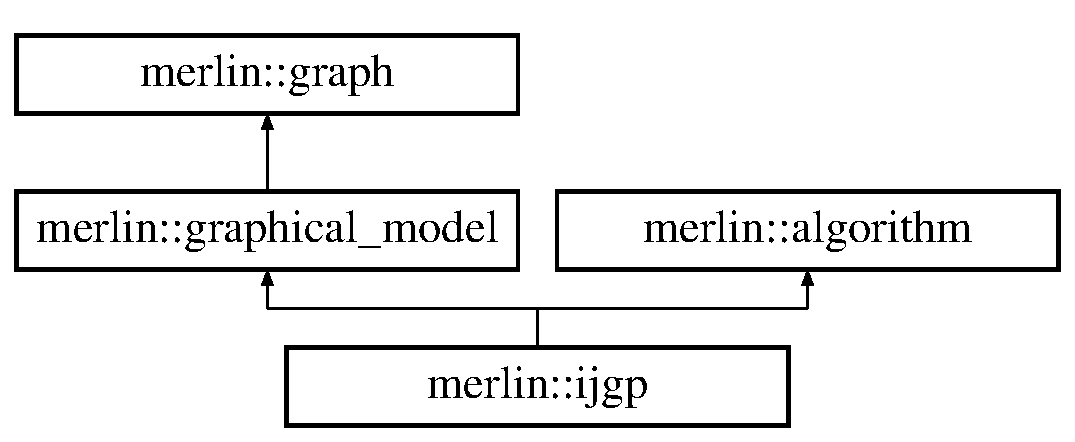
\includegraphics[height=3.000000cm]{classmerlin_1_1ijgp}
\end{center}
\end{figure}
\subsection*{Classes}
\begin{DoxyCompactItemize}
\item 
struct \hyperlink{structmerlin_1_1ijgp_1_1sPair}{s\+Pair}
\begin{DoxyCompactList}\small\item\em Helper class for pairs of sorted indices. \end{DoxyCompactList}\end{DoxyCompactItemize}
\subsection*{Public Types}
\begin{DoxyCompactItemize}
\item 
typedef \hyperlink{classmerlin_1_1graphical__model_ab2b46f09d8142bb68f243ecadbdabb6b}{graphical\+\_\+model\+::findex} \hyperlink{classmerlin_1_1ijgp_af19ce723db28f47c2b35903adbf3d4bc}{findex}\hypertarget{classmerlin_1_1ijgp_af19ce723db28f47c2b35903adbf3d4bc}{}\label{classmerlin_1_1ijgp_af19ce723db28f47c2b35903adbf3d4bc}

\begin{DoxyCompactList}\small\item\em Factor index. \end{DoxyCompactList}\item 
typedef \hyperlink{classmerlin_1_1graphical__model_a275006a490bc09239c12a4d93d53b135}{graphical\+\_\+model\+::vindex} \hyperlink{classmerlin_1_1ijgp_a4c3416087411a776f76a630217515d94}{vindex}\hypertarget{classmerlin_1_1ijgp_a4c3416087411a776f76a630217515d94}{}\label{classmerlin_1_1ijgp_a4c3416087411a776f76a630217515d94}

\begin{DoxyCompactList}\small\item\em Variable index. \end{DoxyCompactList}\item 
typedef \hyperlink{classmerlin_1_1graphical__model_a615e25ec6594615fddfd4c3c4776b99f}{graphical\+\_\+model\+::flist} \hyperlink{classmerlin_1_1ijgp_a3df2ea1455b8c817c6da1630986c2d2c}{flist}\hypertarget{classmerlin_1_1ijgp_a3df2ea1455b8c817c6da1630986c2d2c}{}\label{classmerlin_1_1ijgp_a3df2ea1455b8c817c6da1630986c2d2c}

\begin{DoxyCompactList}\small\item\em Collection of factor indices. \end{DoxyCompactList}\end{DoxyCompactItemize}
\subsection*{Public Member Functions}
\begin{DoxyCompactItemize}
\item 
\hyperlink{classmerlin_1_1ijgp_aeb0d9c018731a8bb51b5b0c3adb3ecfd}{ijgp} ()\hypertarget{classmerlin_1_1ijgp_aeb0d9c018731a8bb51b5b0c3adb3ecfd}{}\label{classmerlin_1_1ijgp_aeb0d9c018731a8bb51b5b0c3adb3ecfd}

\begin{DoxyCompactList}\small\item\em Default constructor. \end{DoxyCompactList}\item 
\hyperlink{classmerlin_1_1ijgp_ac2c784827467ac082b34f717ed5a8b28}{ijgp} (const \hyperlink{classmerlin_1_1graphical__model}{graphical\+\_\+model} \&gm)\hypertarget{classmerlin_1_1ijgp_ac2c784827467ac082b34f717ed5a8b28}{}\label{classmerlin_1_1ijgp_ac2c784827467ac082b34f717ed5a8b28}

\begin{DoxyCompactList}\small\item\em Constructor. \end{DoxyCompactList}\item 
virtual \hyperlink{classmerlin_1_1ijgp}{ijgp} $\ast$ \hyperlink{classmerlin_1_1ijgp_af3ecb1e386de25e892d3246e9fd14a1e}{clone} () const 
\begin{DoxyCompactList}\small\item\em Clone the model. \end{DoxyCompactList}\item 
double \hyperlink{classmerlin_1_1ijgp_aa5813f62d79f2a2c2fcdb24cbc967040}{ub} () const 
\begin{DoxyCompactList}\small\item\em Upper bound on the optimal value. \end{DoxyCompactList}\item 
double \hyperlink{classmerlin_1_1ijgp_ae4313682960f210fc937627446fb70cf}{lb} () const 
\begin{DoxyCompactList}\small\item\em Lower bound on the optimal value. \end{DoxyCompactList}\item 
std\+::vector$<$ size\+\_\+t $>$ \hyperlink{classmerlin_1_1ijgp_af54b5585c353a821071a1ac1f0570679}{best\+\_\+config} () const 
\begin{DoxyCompactList}\small\item\em Best configuration. \end{DoxyCompactList}\item 
double \hyperlink{classmerlin_1_1ijgp_afb334bdd8a981984f1f97ce0d5c58bed}{logZ} () const 
\begin{DoxyCompactList}\small\item\em Log value of the partition function. \end{DoxyCompactList}\item 
double \hyperlink{classmerlin_1_1ijgp_ac0851bfb0a95f0a8ff4b00af298bf743}{log\+Zub} () const 
\begin{DoxyCompactList}\small\item\em Upper bound on the log partition function. \end{DoxyCompactList}\item 
double \hyperlink{classmerlin_1_1ijgp_aa19a722eda63c9471795aff804985d4e}{log\+Zlb} () const 
\begin{DoxyCompactList}\small\item\em Lower bound on the log partition function. \end{DoxyCompactList}\item 
const \hyperlink{classmerlin_1_1factor}{factor} \& \hyperlink{classmerlin_1_1ijgp_a43ba4b5f66a27881b8b6d4a0fed23b3f}{belief} (size\+\_\+t f) const 
\begin{DoxyCompactList}\small\item\em Belief associated with a node of the graph. \end{DoxyCompactList}\item 
const \hyperlink{classmerlin_1_1factor}{factor} \& \hyperlink{classmerlin_1_1ijgp_a950771f418c3fa8980e449c1b081a9cc}{belief} (\hyperlink{classmerlin_1_1variable}{variable} v) const 
\begin{DoxyCompactList}\small\item\em Belief associated with a particular variable. \end{DoxyCompactList}\item 
const \hyperlink{classmerlin_1_1factor}{factor} \& \hyperlink{classmerlin_1_1ijgp_a5506025b0268f56419a472d674faa476}{belief} (\hyperlink{classmerlin_1_1variable__set}{variable\+\_\+set} vs) const 
\begin{DoxyCompactList}\small\item\em Belief associated with a set of variables. \end{DoxyCompactList}\item 
const std\+::vector$<$ \hyperlink{classmerlin_1_1factor}{factor} $>$ \& \hyperlink{classmerlin_1_1ijgp_a031930b83efb5b52a5af5387a18ee0e2}{beliefs} () const 
\begin{DoxyCompactList}\small\item\em Beliefs associated with the variables. \end{DoxyCompactList}\item 
const \hyperlink{classmerlin_1_1graphical__model}{graphical\+\_\+model} \& \hyperlink{classmerlin_1_1ijgp_ac71678e2b148ae0d6b854e07505107fd}{get\+\_\+gm\+\_\+orig} () const \hypertarget{classmerlin_1_1ijgp_ac71678e2b148ae0d6b854e07505107fd}{}\label{classmerlin_1_1ijgp_ac71678e2b148ae0d6b854e07505107fd}

\begin{DoxyCompactList}\small\item\em Access the original graphical model. \end{DoxyCompactList}\item 
void \hyperlink{classmerlin_1_1ijgp_a0054a84cdbf4d9c5d8c93fda1ae17c86}{write\+\_\+solution} (const char $\ast$file\+\_\+name, const std\+::map$<$ size\+\_\+t, size\+\_\+t $>$ \&evidence, const std\+::map$<$ size\+\_\+t, size\+\_\+t $>$ \&old2new, const \hyperlink{classmerlin_1_1graphical__model}{graphical\+\_\+model} \&orig)
\begin{DoxyCompactList}\small\item\em Write the solution to the output file. \end{DoxyCompactList}\item 
virtual void \hyperlink{classmerlin_1_1ijgp_ac255c416a80f2bddab2855e5f66df8bd}{run} ()
\begin{DoxyCompactList}\small\item\em Run the algorithm. \end{DoxyCompactList}\item 
\hyperlink{classmerlin_1_1ijgp_a34acc5c067c4ff887c5f40a2db5f2002}{M\+E\+R\+\_\+\+E\+N\+UM} (Task, PR, M\+AR, M\+AP)\hypertarget{classmerlin_1_1ijgp_a34acc5c067c4ff887c5f40a2db5f2002}{}\label{classmerlin_1_1ijgp_a34acc5c067c4ff887c5f40a2db5f2002}

\begin{DoxyCompactList}\small\item\em Inference tasks supported. \end{DoxyCompactList}\item 
\hyperlink{classmerlin_1_1ijgp_a49319b52721987bed9e9e62fe1e5d26c}{M\+E\+R\+\_\+\+E\+N\+UM} (Property, i\+Bound, Order, Iter, Task, Debug)\hypertarget{classmerlin_1_1ijgp_a49319b52721987bed9e9e62fe1e5d26c}{}\label{classmerlin_1_1ijgp_a49319b52721987bed9e9e62fe1e5d26c}

\begin{DoxyCompactList}\small\item\em Properties of the algorithm. \end{DoxyCompactList}\item 
\hyperlink{classmerlin_1_1ijgp_a185c745e26dbe2061d6d47631907098c}{M\+E\+R\+\_\+\+E\+N\+UM} (Elim\+Op, Max, Sum)\hypertarget{classmerlin_1_1ijgp_a185c745e26dbe2061d6d47631907098c}{}\label{classmerlin_1_1ijgp_a185c745e26dbe2061d6d47631907098c}

\begin{DoxyCompactList}\small\item\em Elimination operators (sum, max). \end{DoxyCompactList}\item 
void \hyperlink{classmerlin_1_1ijgp_a96bd81b7e90ec19825886c83ddfa96c8}{set\+\_\+ibound} (size\+\_\+t i)
\begin{DoxyCompactList}\small\item\em Set the i-\/bound parameter. \end{DoxyCompactList}\item 
size\+\_\+t \hyperlink{classmerlin_1_1ijgp_a8ed83bc7670ed66bbce5e7659031c8b8}{get\+\_\+ibound} () const \hypertarget{classmerlin_1_1ijgp_a8ed83bc7670ed66bbce5e7659031c8b8}{}\label{classmerlin_1_1ijgp_a8ed83bc7670ed66bbce5e7659031c8b8}

\begin{DoxyCompactList}\small\item\em Return the i-\/bound parameter. \end{DoxyCompactList}\item 
void \hyperlink{classmerlin_1_1ijgp_a606c7c45f03321907581254e022ac449}{set\+\_\+order} (const variable\+\_\+order\+\_\+t \&ord)
\begin{DoxyCompactList}\small\item\em Set the variable elimination order. \end{DoxyCompactList}\item 
void \hyperlink{classmerlin_1_1ijgp_a0ef14c891c534a6b5b060921871d2c61}{set\+\_\+order\+\_\+method} (Order\+Method method)
\begin{DoxyCompactList}\small\item\em Set the variable elimination order method. \end{DoxyCompactList}\item 
const variable\+\_\+order\+\_\+t \& \hyperlink{classmerlin_1_1ijgp_a7deef61c7bbda358a1d0ecc6841cff81}{get\+\_\+order} ()\hypertarget{classmerlin_1_1ijgp_a7deef61c7bbda358a1d0ecc6841cff81}{}\label{classmerlin_1_1ijgp_a7deef61c7bbda358a1d0ecc6841cff81}

\begin{DoxyCompactList}\small\item\em Return the variable elimination order. \end{DoxyCompactList}\item 
const std\+::vector$<$ \hyperlink{classmerlin_1_1ijgp_a4c3416087411a776f76a630217515d94}{vindex} $>$ \& \hyperlink{classmerlin_1_1ijgp_a1677ea16e2146f488c0247dcb27278a4}{get\+\_\+pseudo\+\_\+tree} ()\hypertarget{classmerlin_1_1ijgp_a1677ea16e2146f488c0247dcb27278a4}{}\label{classmerlin_1_1ijgp_a1677ea16e2146f488c0247dcb27278a4}

\begin{DoxyCompactList}\small\item\em Return the pseudo tree. \end{DoxyCompactList}\item 
void \hyperlink{classmerlin_1_1ijgp_af01fb5f7e1803fe61e84576ee10c5ca0}{set\+\_\+pseudo\+\_\+tree} (const \hyperlink{classmerlin_1_1vector}{vector}$<$ \hyperlink{classmerlin_1_1ijgp_a4c3416087411a776f76a630217515d94}{vindex} $>$ \&p)
\begin{DoxyCompactList}\small\item\em Set the pseudo tree. \end{DoxyCompactList}\item 
void \hyperlink{classmerlin_1_1ijgp_ae8cc52c3df108d284f464af1918a5b5c}{set\+\_\+graphical\+\_\+model} (const \hyperlink{classmerlin_1_1graphical__model}{graphical\+\_\+model} \&gm)
\begin{DoxyCompactList}\small\item\em Set the graphical model content. \end{DoxyCompactList}\item 
void \hyperlink{classmerlin_1_1ijgp_a6d4dff7d912568950b1bd1b09a406f11}{set\+\_\+graphical\+\_\+model} (const \hyperlink{classmerlin_1_1vector}{vector}$<$ \hyperlink{classmerlin_1_1factor}{factor} $>$ \&fs)
\begin{DoxyCompactList}\small\item\em Set the graphical model content from a list of factors. \end{DoxyCompactList}\item 
virtual void \hyperlink{classmerlin_1_1ijgp_aa092a9e81e288cd2b27b6fc1bb19c1c5}{set\+\_\+properties} (std\+::string opt=std\+::string())
\begin{DoxyCompactList}\small\item\em Set the properties of the algorithm. \end{DoxyCompactList}\item 
\hyperlink{classmerlin_1_1factor}{factor} \hyperlink{classmerlin_1_1ijgp_a7c0bce25459696e44183c6eb6c16c935}{elim} (const \hyperlink{classmerlin_1_1factor}{factor} \&F, const \hyperlink{classmerlin_1_1variable__set}{variable\+\_\+set} \&vs)
\begin{DoxyCompactList}\small\item\em Eliminate a set of variables from a factor. \end{DoxyCompactList}\item 
\hyperlink{classmerlin_1_1factor}{factor} \hyperlink{classmerlin_1_1ijgp_a565027b696c3e8471ad8b8c9e2ce8711}{marg} (const \hyperlink{classmerlin_1_1factor}{factor} \&F, const \hyperlink{classmerlin_1_1variable__set}{variable\+\_\+set} \&vs)
\begin{DoxyCompactList}\small\item\em Compute the marginal over a set of variables. \end{DoxyCompactList}\item 
double \hyperlink{classmerlin_1_1ijgp_a3805cbe0335c203902d3741293c30030}{score} (const \hyperlink{classmerlin_1_1vector}{vector}$<$ \hyperlink{classmerlin_1_1variable__set}{variable\+\_\+set} $>$ \&fin, const \hyperlink{classmerlin_1_1variable}{variable} \&VX, size\+\_\+t i, size\+\_\+t j)
\begin{DoxyCompactList}\small\item\em Scoring function for bucket aggregation. \end{DoxyCompactList}\item 
void \hyperlink{classmerlin_1_1ijgp_a8300ed201011020d5dffe498d3de44c1}{init} ()\hypertarget{classmerlin_1_1ijgp_a8300ed201011020d5dffe498d3de44c1}{}\label{classmerlin_1_1ijgp_a8300ed201011020d5dffe498d3de44c1}

\begin{DoxyCompactList}\small\item\em Create the mini-\/bucket based join-\/graph (symbols only). \end{DoxyCompactList}\item 
\hyperlink{classmerlin_1_1factor}{factor} \hyperlink{classmerlin_1_1ijgp_a1d7412044771f675633ec1ff12c26eaf}{calc\+\_\+belief} (\hyperlink{classmerlin_1_1ijgp_af19ce723db28f47c2b35903adbf3d4bc}{findex} a)
\begin{DoxyCompactList}\small\item\em Compute the belief of a cluster. \end{DoxyCompactList}\item 
\hyperlink{classmerlin_1_1factor}{factor} \hyperlink{classmerlin_1_1ijgp_a19bb2cc8542ce62c994b914b456ae0e3}{calc\+\_\+belief} (\hyperlink{classmerlin_1_1ijgp_af19ce723db28f47c2b35903adbf3d4bc}{findex} a, size\+\_\+t b)
\begin{DoxyCompactList}\small\item\em Compute the belief of a cluster excluding an incoming message. \end{DoxyCompactList}\item 
\hyperlink{classmerlin_1_1factor}{factor} \hyperlink{classmerlin_1_1ijgp_aea8e02bac8d7c6f5577bb4269b253726}{incoming} (\hyperlink{classmerlin_1_1ijgp_af19ce723db28f47c2b35903adbf3d4bc}{findex} a)
\begin{DoxyCompactList}\small\item\em Compute the belief of a cluster excluding backward messages. \end{DoxyCompactList}\item 
void \hyperlink{classmerlin_1_1ijgp_a61caa150c8d8bdfb7e26640a5d62ebd6}{forward} ()\hypertarget{classmerlin_1_1ijgp_a61caa150c8d8bdfb7e26640a5d62ebd6}{}\label{classmerlin_1_1ijgp_a61caa150c8d8bdfb7e26640a5d62ebd6}

\begin{DoxyCompactList}\small\item\em Forward (top-\/down) message passing. \end{DoxyCompactList}\item 
void \hyperlink{classmerlin_1_1ijgp_a8b80c5fed9c242c85200c84885282287}{backward} ()\hypertarget{classmerlin_1_1ijgp_a8b80c5fed9c242c85200c84885282287}{}\label{classmerlin_1_1ijgp_a8b80c5fed9c242c85200c84885282287}

\begin{DoxyCompactList}\small\item\em Backward (bottom-\/up) message passing. \end{DoxyCompactList}\item 
void \hyperlink{classmerlin_1_1ijgp_ac44f5db012d6b2ef76aae27a6eaff0da}{update} ()\hypertarget{classmerlin_1_1ijgp_ac44f5db012d6b2ef76aae27a6eaff0da}{}\label{classmerlin_1_1ijgp_ac44f5db012d6b2ef76aae27a6eaff0da}

\begin{DoxyCompactList}\small\item\em Update the beliefs (marginals or max-\/marginals) for each variable. \end{DoxyCompactList}\item 
void \hyperlink{classmerlin_1_1ijgp_a76bf2137d3b82d923d1d4dcbd5353b21}{propagate} (size\+\_\+t n\+Iter, double stop\+Time=-\/1, double stop\+Obj=-\/1)
\begin{DoxyCompactList}\small\item\em Iterative message passing over the join graph. \end{DoxyCompactList}\end{DoxyCompactItemize}
\subsection*{Protected Attributes}
\begin{DoxyCompactItemize}
\item 
\hyperlink{classmerlin_1_1graphical__model}{graphical\+\_\+model} \hyperlink{classmerlin_1_1ijgp_a94a5a3960cccee65a302db50d3157390}{m\+\_\+gmo}\hypertarget{classmerlin_1_1ijgp_a94a5a3960cccee65a302db50d3157390}{}\label{classmerlin_1_1ijgp_a94a5a3960cccee65a302db50d3157390}

\begin{DoxyCompactList}\small\item\em Original graphical model. \end{DoxyCompactList}\item 
size\+\_\+t \hyperlink{classmerlin_1_1ijgp_a277f1da495f57da65fad7903dba33e88}{num\+\_\+iter}\hypertarget{classmerlin_1_1ijgp_a277f1da495f57da65fad7903dba33e88}{}\label{classmerlin_1_1ijgp_a277f1da495f57da65fad7903dba33e88}

\begin{DoxyCompactList}\small\item\em Number of iterations. \end{DoxyCompactList}\item 
Task \hyperlink{classmerlin_1_1ijgp_a95e03dea51e4dc87d7a48a50415df005}{m\+\_\+task}\hypertarget{classmerlin_1_1ijgp_a95e03dea51e4dc87d7a48a50415df005}{}\label{classmerlin_1_1ijgp_a95e03dea51e4dc87d7a48a50415df005}

\begin{DoxyCompactList}\small\item\em Inference task. \end{DoxyCompactList}\item 
Elim\+Op \hyperlink{classmerlin_1_1ijgp_a4a80b800e11190f3eb790cfd9899dad7}{m\+\_\+elim\+\_\+op}\hypertarget{classmerlin_1_1ijgp_a4a80b800e11190f3eb790cfd9899dad7}{}\label{classmerlin_1_1ijgp_a4a80b800e11190f3eb790cfd9899dad7}

\begin{DoxyCompactList}\small\item\em Elimination operator. \end{DoxyCompactList}\item 
size\+\_\+t \hyperlink{classmerlin_1_1ijgp_aa15a0be92dea2367ba5686b3f9aebebe}{m\+\_\+ibound}\hypertarget{classmerlin_1_1ijgp_aa15a0be92dea2367ba5686b3f9aebebe}{}\label{classmerlin_1_1ijgp_aa15a0be92dea2367ba5686b3f9aebebe}

\begin{DoxyCompactList}\small\item\em i-\/bound parameter \end{DoxyCompactList}\item 
double \hyperlink{classmerlin_1_1ijgp_a32298dfd2e209e8b6ffb6814c1116b75}{m\+\_\+log\+\_\+z}\hypertarget{classmerlin_1_1ijgp_a32298dfd2e209e8b6ffb6814c1116b75}{}\label{classmerlin_1_1ijgp_a32298dfd2e209e8b6ffb6814c1116b75}

\begin{DoxyCompactList}\small\item\em Log partition function value. \end{DoxyCompactList}\item 
variable\+\_\+order\+\_\+t \hyperlink{classmerlin_1_1ijgp_a2d48b9031e13697c21946e9c7ed836b1}{m\+\_\+order}\hypertarget{classmerlin_1_1ijgp_a2d48b9031e13697c21946e9c7ed836b1}{}\label{classmerlin_1_1ijgp_a2d48b9031e13697c21946e9c7ed836b1}

\begin{DoxyCompactList}\small\item\em Variable elimination order. \end{DoxyCompactList}\item 
Order\+Method \hyperlink{classmerlin_1_1ijgp_a768a3aa7d07f7c110453441c0358e8bb}{m\+\_\+order\+\_\+method}\hypertarget{classmerlin_1_1ijgp_a768a3aa7d07f7c110453441c0358e8bb}{}\label{classmerlin_1_1ijgp_a768a3aa7d07f7c110453441c0358e8bb}

\begin{DoxyCompactList}\small\item\em Ordering method. \end{DoxyCompactList}\item 
std\+::vector$<$ \hyperlink{classmerlin_1_1ijgp_a4c3416087411a776f76a630217515d94}{vindex} $>$ \hyperlink{classmerlin_1_1ijgp_a5b387b54c771f44f2a1bf29b397f6f97}{m\+\_\+parents}\hypertarget{classmerlin_1_1ijgp_a5b387b54c771f44f2a1bf29b397f6f97}{}\label{classmerlin_1_1ijgp_a5b387b54c771f44f2a1bf29b397f6f97}

\begin{DoxyCompactList}\small\item\em Pseudo tree. \end{DoxyCompactList}\item 
std\+::vector$<$ \hyperlink{classmerlin_1_1factor}{factor} $>$ \hyperlink{classmerlin_1_1ijgp_a1899ac5a6fa45ae93d10fed4ae78e6ba}{m\+\_\+beliefs}\hypertarget{classmerlin_1_1ijgp_a1899ac5a6fa45ae93d10fed4ae78e6ba}{}\label{classmerlin_1_1ijgp_a1899ac5a6fa45ae93d10fed4ae78e6ba}

\begin{DoxyCompactList}\small\item\em Marginals (or beliefs) \end{DoxyCompactList}\item 
std\+::vector$<$ size\+\_\+t $>$ \hyperlink{classmerlin_1_1ijgp_a6f00b802c54c7d225001577edb51bbc8}{m\+\_\+best\+\_\+config}\hypertarget{classmerlin_1_1ijgp_a6f00b802c54c7d225001577edb51bbc8}{}\label{classmerlin_1_1ijgp_a6f00b802c54c7d225001577edb51bbc8}

\begin{DoxyCompactList}\small\item\em M\+AP assignment. \end{DoxyCompactList}\item 
double \hyperlink{classmerlin_1_1ijgp_a5665048f86025d11b0c4fe40eeb4ddfb}{m\+\_\+lb}\hypertarget{classmerlin_1_1ijgp_a5665048f86025d11b0c4fe40eeb4ddfb}{}\label{classmerlin_1_1ijgp_a5665048f86025d11b0c4fe40eeb4ddfb}

\begin{DoxyCompactList}\small\item\em Lower bound (ie, value of the M\+AP assignment) \end{DoxyCompactList}\end{DoxyCompactItemize}
\subsection*{Additional Inherited Members}


\subsection{Detailed Description}
Iterative Join-\/\+Graph Propagation (I\+J\+GP)

Based on \mbox{[}Dechter and Mateescu, 2002\mbox{]} and \mbox{[}Marinescu, Kask and Dechter, 2003\mbox{]}

Tasks supported\+: M\+AR and M\+AP

I\+J\+GP is parameterized by an i-\/bound which limits the size of each cluster in the join-\/graph to at most i distict variables. Clearly I\+J\+G\+P(1) is equivalent with Loopy Belief Propagation, while I\+J\+G\+P(w$\ast$) is equivalent with the Join-\/\+Tree algorithm, hence exact.

The join-\/graph used by I\+J\+GP is obtained by running the mini-\/bucket algorithm schematically (ie, without computing the actual messages, only their scopes) and then connecting the mini-\/buckets residing in the same bucket. Messages are then propagated along the join-\/graph edges, following a top-\/down or bottom-\/up schedule.

Note that I\+J\+GP is only used for M\+AR (sum-\/prod) and M\+AP (max-\/prod) tasks. It doesn\textquotesingle{}t compute an upper-\/bound (on the partition function, or the M\+AP value) because of overcounting. Therefore, logZ reported during the execution of the algorithm shouldn\textquotesingle{}t be used as a valid measure for bounding (ignore). For valid bounding, use the W\+MB algorithm implemented in this library. 

Definition at line 58 of file ijgp.\+h.



\subsection{Member Function Documentation}
\index{merlin\+::ijgp@{merlin\+::ijgp}!belief@{belief}}
\index{belief@{belief}!merlin\+::ijgp@{merlin\+::ijgp}}
\subsubsection[{\texorpdfstring{belief(size\+\_\+t f) const }{belief(size_t f) const }}]{\setlength{\rightskip}{0pt plus 5cm}const {\bf factor}\& merlin\+::ijgp\+::belief (
\begin{DoxyParamCaption}
\item[{size\+\_\+t}]{i}
\end{DoxyParamCaption}
) const\hspace{0.3cm}{\ttfamily [inline]}, {\ttfamily [virtual]}}\hypertarget{classmerlin_1_1ijgp_a43ba4b5f66a27881b8b6d4a0fed23b3f}{}\label{classmerlin_1_1ijgp_a43ba4b5f66a27881b8b6d4a0fed23b3f}


Belief associated with a node of the graph. 

\begin{DoxyReturn}{Returns}
the belief associated with a node of the graph. Nodes correspond typically to variables. The belied is a function represented by the Factor class. 
\end{DoxyReturn}

\begin{DoxyParams}{Parameters}
{\em i} & The index of the node in the graph (from 0) \\
\hline
\end{DoxyParams}


Implements \hyperlink{classmerlin_1_1algorithm_a617b3e562037a7716f7cfd6cf1e55c19}{merlin\+::algorithm}.



Definition at line 112 of file ijgp.\+h.



References m\+\_\+beliefs.



Referenced by run(), and write\+\_\+solution().

\index{merlin\+::ijgp@{merlin\+::ijgp}!belief@{belief}}
\index{belief@{belief}!merlin\+::ijgp@{merlin\+::ijgp}}
\subsubsection[{\texorpdfstring{belief(variable v) const }{belief(variable v) const }}]{\setlength{\rightskip}{0pt plus 5cm}const {\bf factor}\& merlin\+::ijgp\+::belief (
\begin{DoxyParamCaption}
\item[{{\bf variable}}]{v}
\end{DoxyParamCaption}
) const\hspace{0.3cm}{\ttfamily [inline]}, {\ttfamily [virtual]}}\hypertarget{classmerlin_1_1ijgp_a950771f418c3fa8980e449c1b081a9cc}{}\label{classmerlin_1_1ijgp_a950771f418c3fa8980e449c1b081a9cc}


Belief associated with a particular variable. 


\begin{DoxyParams}{Parameters}
{\em v} & The variable to compute the belief of \\
\hline
\end{DoxyParams}
\begin{DoxyReturn}{Returns}
the belief associated with a particular variable in the graphical model. The belief is a function represented by the Factor class. 
\end{DoxyReturn}


Implements \hyperlink{classmerlin_1_1algorithm_adc966d1ed7ac479754441bab138f7efa}{merlin\+::algorithm}.



Definition at line 115 of file ijgp.\+h.



References m\+\_\+beliefs.

\index{merlin\+::ijgp@{merlin\+::ijgp}!belief@{belief}}
\index{belief@{belief}!merlin\+::ijgp@{merlin\+::ijgp}}
\subsubsection[{\texorpdfstring{belief(variable\+\_\+set vs) const }{belief(variable_set vs) const }}]{\setlength{\rightskip}{0pt plus 5cm}const {\bf factor}\& merlin\+::ijgp\+::belief (
\begin{DoxyParamCaption}
\item[{{\bf variable\+\_\+set}}]{vs}
\end{DoxyParamCaption}
) const\hspace{0.3cm}{\ttfamily [inline]}, {\ttfamily [virtual]}}\hypertarget{classmerlin_1_1ijgp_a5506025b0268f56419a472d674faa476}{}\label{classmerlin_1_1ijgp_a5506025b0268f56419a472d674faa476}


Belief associated with a set of variables. 


\begin{DoxyParams}{Parameters}
{\em vs} & The set of variables to compute the belief of \\
\hline
\end{DoxyParams}
\begin{DoxyReturn}{Returns}
the belief associated with a set of variables in the graphical model. The belief is a function represented by the Factor class. 
\end{DoxyReturn}


Implements \hyperlink{classmerlin_1_1algorithm_ad19b068623b85ad1cd4bb262e7bcfc6f}{merlin\+::algorithm}.



Definition at line 118 of file ijgp.\+h.

\index{merlin\+::ijgp@{merlin\+::ijgp}!beliefs@{beliefs}}
\index{beliefs@{beliefs}!merlin\+::ijgp@{merlin\+::ijgp}}
\subsubsection[{\texorpdfstring{beliefs() const }{beliefs() const }}]{\setlength{\rightskip}{0pt plus 5cm}const std\+::vector$<${\bf factor}$>$\& merlin\+::ijgp\+::beliefs (
\begin{DoxyParamCaption}
{}
\end{DoxyParamCaption}
) const\hspace{0.3cm}{\ttfamily [inline]}, {\ttfamily [virtual]}}\hypertarget{classmerlin_1_1ijgp_a031930b83efb5b52a5af5387a18ee0e2}{}\label{classmerlin_1_1ijgp_a031930b83efb5b52a5af5387a18ee0e2}


Beliefs associated with the variables. 

\begin{DoxyReturn}{Returns}
the beliefs associated with the variables in the graphical model (one belief for each of the variables). The output vector is indexed by the same indexes used for the variables. 
\end{DoxyReturn}


Implements \hyperlink{classmerlin_1_1algorithm_a0b70d8fe87b32bca601a3d116b673b47}{merlin\+::algorithm}.



Definition at line 121 of file ijgp.\+h.



References m\+\_\+beliefs.

\index{merlin\+::ijgp@{merlin\+::ijgp}!best\+\_\+config@{best\+\_\+config}}
\index{best\+\_\+config@{best\+\_\+config}!merlin\+::ijgp@{merlin\+::ijgp}}
\subsubsection[{\texorpdfstring{best\+\_\+config() const }{best_config() const }}]{\setlength{\rightskip}{0pt plus 5cm}std\+::vector$<$size\+\_\+t$>$ merlin\+::ijgp\+::best\+\_\+config (
\begin{DoxyParamCaption}
{}
\end{DoxyParamCaption}
) const\hspace{0.3cm}{\ttfamily [inline]}, {\ttfamily [virtual]}}\hypertarget{classmerlin_1_1ijgp_af54b5585c353a821071a1ac1f0570679}{}\label{classmerlin_1_1ijgp_af54b5585c353a821071a1ac1f0570679}


Best configuration. 

\begin{DoxyReturn}{Returns}
a vector containing the best configuration of the variables (i.\+e., variable value assignments) found so far. It is specific to optimization tasks (e.\+g., M\+AP, Marginal M\+AP). 
\end{DoxyReturn}


Implements \hyperlink{classmerlin_1_1algorithm_a3d84d2595e6235db93a9bb3e1a012e48}{merlin\+::algorithm}.



Definition at line 98 of file ijgp.\+h.



References m\+\_\+best\+\_\+config.

\index{merlin\+::ijgp@{merlin\+::ijgp}!calc\+\_\+belief@{calc\+\_\+belief}}
\index{calc\+\_\+belief@{calc\+\_\+belief}!merlin\+::ijgp@{merlin\+::ijgp}}
\subsubsection[{\texorpdfstring{calc\+\_\+belief(findex a)}{calc_belief(findex a)}}]{\setlength{\rightskip}{0pt plus 5cm}{\bf factor} merlin\+::ijgp\+::calc\+\_\+belief (
\begin{DoxyParamCaption}
\item[{{\bf findex}}]{a}
\end{DoxyParamCaption}
)\hspace{0.3cm}{\ttfamily [inline]}}\hypertarget{classmerlin_1_1ijgp_a1d7412044771f675633ec1ff12c26eaf}{}\label{classmerlin_1_1ijgp_a1d7412044771f675633ec1ff12c26eaf}


Compute the belief of a cluster. 


\begin{DoxyParams}{Parameters}
{\em a} & The index of the cluster \\
\hline
\end{DoxyParams}
\begin{DoxyReturn}{Returns}
the factor representing the belief of the cluster. 
\end{DoxyReturn}


Definition at line 820 of file ijgp.\+h.



References merlin\+::graphical\+\_\+model\+::m\+\_\+factors.



Referenced by backward(), forward(), and update().

\index{merlin\+::ijgp@{merlin\+::ijgp}!calc\+\_\+belief@{calc\+\_\+belief}}
\index{calc\+\_\+belief@{calc\+\_\+belief}!merlin\+::ijgp@{merlin\+::ijgp}}
\subsubsection[{\texorpdfstring{calc\+\_\+belief(findex a, size\+\_\+t b)}{calc_belief(findex a, size_t b)}}]{\setlength{\rightskip}{0pt plus 5cm}{\bf factor} merlin\+::ijgp\+::calc\+\_\+belief (
\begin{DoxyParamCaption}
\item[{{\bf findex}}]{a, }
\item[{size\+\_\+t}]{b}
\end{DoxyParamCaption}
)\hspace{0.3cm}{\ttfamily [inline]}}\hypertarget{classmerlin_1_1ijgp_a19bb2cc8542ce62c994b914b456ae0e3}{}\label{classmerlin_1_1ijgp_a19bb2cc8542ce62c994b914b456ae0e3}


Compute the belief of a cluster excluding an incoming message. 


\begin{DoxyParams}{Parameters}
{\em a} & The index of the cluster to compute the belief of \\
\hline
{\em b} & The index of the cluster sending the incoming message \\
\hline
\end{DoxyParams}
\begin{DoxyReturn}{Returns}
the factor representing the belief of cluster {\itshape a} excluding the incoming message from {\itshape b} to {\itshape a}. 
\end{DoxyReturn}


Definition at line 850 of file ijgp.\+h.



References merlin\+::graphical\+\_\+model\+::m\+\_\+factors.

\index{merlin\+::ijgp@{merlin\+::ijgp}!clone@{clone}}
\index{clone@{clone}!merlin\+::ijgp@{merlin\+::ijgp}}
\subsubsection[{\texorpdfstring{clone() const }{clone() const }}]{\setlength{\rightskip}{0pt plus 5cm}virtual {\bf ijgp}$\ast$ merlin\+::ijgp\+::clone (
\begin{DoxyParamCaption}
{}
\end{DoxyParamCaption}
) const\hspace{0.3cm}{\ttfamily [inline]}, {\ttfamily [virtual]}}\hypertarget{classmerlin_1_1ijgp_af3ecb1e386de25e892d3246e9fd14a1e}{}\label{classmerlin_1_1ijgp_af3ecb1e386de25e892d3246e9fd14a1e}


Clone the model. 

\begin{DoxyReturn}{Returns}
the pointer to the object containing the cloned model. 
\end{DoxyReturn}


Implements \hyperlink{classmerlin_1_1algorithm_a10f787e24c1fd5ec92c26b18efb0b8db}{merlin\+::algorithm}.



Definition at line 85 of file ijgp.\+h.



References ijgp().

\index{merlin\+::ijgp@{merlin\+::ijgp}!elim@{elim}}
\index{elim@{elim}!merlin\+::ijgp@{merlin\+::ijgp}}
\subsubsection[{\texorpdfstring{elim(const factor \&\+F, const variable\+\_\+set \&vs)}{elim(const factor &F, const variable_set &vs)}}]{\setlength{\rightskip}{0pt plus 5cm}{\bf factor} merlin\+::ijgp\+::elim (
\begin{DoxyParamCaption}
\item[{const {\bf factor} \&}]{F, }
\item[{const {\bf variable\+\_\+set} \&}]{vs}
\end{DoxyParamCaption}
)\hspace{0.3cm}{\ttfamily [inline]}}\hypertarget{classmerlin_1_1ijgp_a7c0bce25459696e44183c6eb6c16c935}{}\label{classmerlin_1_1ijgp_a7c0bce25459696e44183c6eb6c16c935}


Eliminate a set of variables from a factor. 


\begin{DoxyParams}{Parameters}
{\em F} & The reference of the factor to eliminate from \\
\hline
{\em vs} & The set of variables to be eliminated \\
\hline
\end{DoxyParams}
\begin{DoxyReturn}{Returns}
the factor resulted from eliminating the set of variables. 
\end{DoxyReturn}


Definition at line 426 of file ijgp.\+h.



References merlin\+::factor\+::max(), and merlin\+::factor\+::sum().



Referenced by backward(), and forward().

\index{merlin\+::ijgp@{merlin\+::ijgp}!incoming@{incoming}}
\index{incoming@{incoming}!merlin\+::ijgp@{merlin\+::ijgp}}
\subsubsection[{\texorpdfstring{incoming(findex a)}{incoming(findex a)}}]{\setlength{\rightskip}{0pt plus 5cm}{\bf factor} merlin\+::ijgp\+::incoming (
\begin{DoxyParamCaption}
\item[{{\bf findex}}]{a}
\end{DoxyParamCaption}
)\hspace{0.3cm}{\ttfamily [inline]}}\hypertarget{classmerlin_1_1ijgp_aea8e02bac8d7c6f5577bb4269b253726}{}\label{classmerlin_1_1ijgp_aea8e02bac8d7c6f5577bb4269b253726}


Compute the belief of a cluster excluding backward messages. 


\begin{DoxyParams}{Parameters}
{\em a} & The index of the cluster to compute the belief of \\
\hline
\end{DoxyParams}
\begin{DoxyReturn}{Returns}
the factor representing the belief of cluster {\itshape a} excluding the backward messages from clusters below {\itshape a}. 
\end{DoxyReturn}


Definition at line 881 of file ijgp.\+h.



References merlin\+::graphical\+\_\+model\+::m\+\_\+factors.



Referenced by update().

\index{merlin\+::ijgp@{merlin\+::ijgp}!lb@{lb}}
\index{lb@{lb}!merlin\+::ijgp@{merlin\+::ijgp}}
\subsubsection[{\texorpdfstring{lb() const }{lb() const }}]{\setlength{\rightskip}{0pt plus 5cm}double merlin\+::ijgp\+::lb (
\begin{DoxyParamCaption}
{}
\end{DoxyParamCaption}
) const\hspace{0.3cm}{\ttfamily [inline]}, {\ttfamily [virtual]}}\hypertarget{classmerlin_1_1ijgp_ae4313682960f210fc937627446fb70cf}{}\label{classmerlin_1_1ijgp_ae4313682960f210fc937627446fb70cf}


Lower bound on the optimal value. 

\begin{DoxyReturn}{Returns}
a lower bound on the optimal value defined by the inference task if available. 
\end{DoxyReturn}


Implements \hyperlink{classmerlin_1_1algorithm_adc3f19055c0466682b5577049df14863}{merlin\+::algorithm}.



Definition at line 95 of file ijgp.\+h.

\index{merlin\+::ijgp@{merlin\+::ijgp}!logZ@{logZ}}
\index{logZ@{logZ}!merlin\+::ijgp@{merlin\+::ijgp}}
\subsubsection[{\texorpdfstring{log\+Z() const }{logZ() const }}]{\setlength{\rightskip}{0pt plus 5cm}double merlin\+::ijgp\+::logZ (
\begin{DoxyParamCaption}
{}
\end{DoxyParamCaption}
) const\hspace{0.3cm}{\ttfamily [inline]}, {\ttfamily [virtual]}}\hypertarget{classmerlin_1_1ijgp_afb334bdd8a981984f1f97ce0d5c58bed}{}\label{classmerlin_1_1ijgp_afb334bdd8a981984f1f97ce0d5c58bed}


Log value of the partition function. 

\begin{DoxyReturn}{Returns}
an estimate the log parition function. If the inference algorithm is an exact one then the return value is the exact log value of the partition function. 
\end{DoxyReturn}


Implements \hyperlink{classmerlin_1_1algorithm_a26eadf71ba80c0a9cd3d7cfe18c95717}{merlin\+::algorithm}.



Definition at line 102 of file ijgp.\+h.



References m\+\_\+log\+\_\+z.

\index{merlin\+::ijgp@{merlin\+::ijgp}!log\+Zlb@{log\+Zlb}}
\index{log\+Zlb@{log\+Zlb}!merlin\+::ijgp@{merlin\+::ijgp}}
\subsubsection[{\texorpdfstring{log\+Zlb() const }{logZlb() const }}]{\setlength{\rightskip}{0pt plus 5cm}double merlin\+::ijgp\+::log\+Zlb (
\begin{DoxyParamCaption}
{}
\end{DoxyParamCaption}
) const\hspace{0.3cm}{\ttfamily [inline]}, {\ttfamily [virtual]}}\hypertarget{classmerlin_1_1ijgp_aa19a722eda63c9471795aff804985d4e}{}\label{classmerlin_1_1ijgp_aa19a722eda63c9471795aff804985d4e}


Lower bound on the log partition function. 

\begin{DoxyReturn}{Returns}
a lower bound on the log value of the parition function. 
\end{DoxyReturn}


Implements \hyperlink{classmerlin_1_1algorithm_a14d163a3e90a898487d3a6e273e1fecf}{merlin\+::algorithm}.



Definition at line 108 of file ijgp.\+h.



References m\+\_\+log\+\_\+z.

\index{merlin\+::ijgp@{merlin\+::ijgp}!log\+Zub@{log\+Zub}}
\index{log\+Zub@{log\+Zub}!merlin\+::ijgp@{merlin\+::ijgp}}
\subsubsection[{\texorpdfstring{log\+Zub() const }{logZub() const }}]{\setlength{\rightskip}{0pt plus 5cm}double merlin\+::ijgp\+::log\+Zub (
\begin{DoxyParamCaption}
{}
\end{DoxyParamCaption}
) const\hspace{0.3cm}{\ttfamily [inline]}, {\ttfamily [virtual]}}\hypertarget{classmerlin_1_1ijgp_ac0851bfb0a95f0a8ff4b00af298bf743}{}\label{classmerlin_1_1ijgp_ac0851bfb0a95f0a8ff4b00af298bf743}


Upper bound on the log partition function. 

\begin{DoxyReturn}{Returns}
an upper bound on the log value of the parition function. Most inference algorithms implemented in merlin support upper bounds on the log partition function. 
\end{DoxyReturn}


Implements \hyperlink{classmerlin_1_1algorithm_aeece2e8f008bcc94697353088c4afefe}{merlin\+::algorithm}.



Definition at line 105 of file ijgp.\+h.



References m\+\_\+log\+\_\+z.

\index{merlin\+::ijgp@{merlin\+::ijgp}!marg@{marg}}
\index{marg@{marg}!merlin\+::ijgp@{merlin\+::ijgp}}
\subsubsection[{\texorpdfstring{marg(const factor \&\+F, const variable\+\_\+set \&vs)}{marg(const factor &F, const variable_set &vs)}}]{\setlength{\rightskip}{0pt plus 5cm}{\bf factor} merlin\+::ijgp\+::marg (
\begin{DoxyParamCaption}
\item[{const {\bf factor} \&}]{F, }
\item[{const {\bf variable\+\_\+set} \&}]{vs}
\end{DoxyParamCaption}
)\hspace{0.3cm}{\ttfamily [inline]}}\hypertarget{classmerlin_1_1ijgp_a565027b696c3e8471ad8b8c9e2ce8711}{}\label{classmerlin_1_1ijgp_a565027b696c3e8471ad8b8c9e2ce8711}


Compute the marginal over a set of variables. 


\begin{DoxyParams}{Parameters}
{\em F} & The reference of the factor to marginalize over \\
\hline
{\em vs} & The set of variables representing the scope of the marginal \\
\hline
\end{DoxyParams}
\begin{DoxyReturn}{Returns}
the factor representing the marginal over the set of variables. 
\end{DoxyReturn}


Definition at line 444 of file ijgp.\+h.



References merlin\+::factor\+::marginal(), and merlin\+::factor\+::maxmarginal().



Referenced by update().

\index{merlin\+::ijgp@{merlin\+::ijgp}!propagate@{propagate}}
\index{propagate@{propagate}!merlin\+::ijgp@{merlin\+::ijgp}}
\subsubsection[{\texorpdfstring{propagate(size\+\_\+t n\+Iter, double stop\+Time=-\/1, double stop\+Obj=-\/1)}{propagate(size_t nIter, double stopTime=-1, double stopObj=-1)}}]{\setlength{\rightskip}{0pt plus 5cm}void merlin\+::ijgp\+::propagate (
\begin{DoxyParamCaption}
\item[{size\+\_\+t}]{n\+Iter, }
\item[{double}]{stop\+Time = {\ttfamily -\/1}, }
\item[{double}]{stop\+Obj = {\ttfamily -\/1}}
\end{DoxyParamCaption}
)\hspace{0.3cm}{\ttfamily [inline]}}\hypertarget{classmerlin_1_1ijgp_a76bf2137d3b82d923d1d4dcbd5353b21}{}\label{classmerlin_1_1ijgp_a76bf2137d3b82d923d1d4dcbd5353b21}


Iterative message passing over the join graph. 


\begin{DoxyParams}{Parameters}
{\em n\+Iter} & The number of iterations \\
\hline
{\em stop\+Time} & The time limit \\
\hline
{\em stop\+Obj} & The error tolerance (ie, difference between objective values) \\
\hline
\end{DoxyParams}


Definition at line 1070 of file ijgp.\+h.



References backward(), forward(), m\+\_\+log\+\_\+z, merlin\+::algorithm\+::m\+\_\+start\+\_\+time, M\+E\+R\+L\+I\+N\+\_\+\+D\+O\+U\+B\+L\+E\+\_\+\+P\+R\+E\+C\+I\+S\+I\+ON, and update().



Referenced by run().

\index{merlin\+::ijgp@{merlin\+::ijgp}!run@{run}}
\index{run@{run}!merlin\+::ijgp@{merlin\+::ijgp}}
\subsubsection[{\texorpdfstring{run()}{run()}}]{\setlength{\rightskip}{0pt plus 5cm}virtual void merlin\+::ijgp\+::run (
\begin{DoxyParamCaption}
{}
\end{DoxyParamCaption}
)\hspace{0.3cm}{\ttfamily [inline]}, {\ttfamily [virtual]}}\hypertarget{classmerlin_1_1ijgp_ac255c416a80f2bddab2855e5f66df8bd}{}\label{classmerlin_1_1ijgp_ac255c416a80f2bddab2855e5f66df8bd}


Run the algorithm. 

Solves a probabilistic inference task. 

Implements \hyperlink{classmerlin_1_1algorithm_a6a701ee51b3d1009041702129161b0de}{merlin\+::algorithm}.



Definition at line 204 of file ijgp.\+h.



References belief(), init(), merlin\+::graphical\+\_\+model\+::log\+P(), m\+\_\+best\+\_\+config, m\+\_\+gmo, m\+\_\+lb, m\+\_\+log\+\_\+z, merlin\+::algorithm\+::m\+\_\+start\+\_\+time, m\+\_\+task, M\+E\+R\+\_\+\+E\+N\+U\+M(), M\+E\+R\+L\+I\+N\+\_\+\+D\+O\+U\+B\+L\+E\+\_\+\+P\+R\+E\+C\+I\+S\+I\+ON, num\+\_\+iter, merlin\+::graphical\+\_\+model\+::nvar(), propagate(), merlin\+::variable\+::states(), and merlin\+::graphical\+\_\+model\+::var().



Referenced by Merlin\+::run().

\index{merlin\+::ijgp@{merlin\+::ijgp}!score@{score}}
\index{score@{score}!merlin\+::ijgp@{merlin\+::ijgp}}
\subsubsection[{\texorpdfstring{score(const vector$<$ variable\+\_\+set $>$ \&fin, const variable \&\+V\+X, size\+\_\+t i, size\+\_\+t j)}{score(const vector< variable_set > &fin, const variable &VX, size_t i, size_t j)}}]{\setlength{\rightskip}{0pt plus 5cm}double merlin\+::ijgp\+::score (
\begin{DoxyParamCaption}
\item[{const {\bf vector}$<$ {\bf variable\+\_\+set} $>$ \&}]{fin, }
\item[{const {\bf variable} \&}]{VX, }
\item[{size\+\_\+t}]{i, }
\item[{size\+\_\+t}]{j}
\end{DoxyParamCaption}
)\hspace{0.3cm}{\ttfamily [inline]}}\hypertarget{classmerlin_1_1ijgp_a3805cbe0335c203902d3741293c30030}{}\label{classmerlin_1_1ijgp_a3805cbe0335c203902d3741293c30030}


Scoring function for bucket aggregation. 


\begin{DoxyParams}{Parameters}
{\em fin} & The set of factor scopes containing the pair (i,j) to be aggregated \\
\hline
{\em VX} & The bucket variable \\
\hline
{\em i} & The index of first scope \\
\hline
{\em j} & The index of the second pair \\
\hline
\end{DoxyParams}
\begin{DoxyReturn}{Returns}
the score that corresponds to aggregating the two scopes. It returns -\/3 if unable to combine, -\/1 for scope only aggregation, and otherwise a positive double score. 
\end{DoxyReturn}


Definition at line 467 of file ijgp.\+h.



References merlin\+::variable\+\_\+set\+::nvar().



Referenced by init().

\index{merlin\+::ijgp@{merlin\+::ijgp}!set\+\_\+graphical\+\_\+model@{set\+\_\+graphical\+\_\+model}}
\index{set\+\_\+graphical\+\_\+model@{set\+\_\+graphical\+\_\+model}!merlin\+::ijgp@{merlin\+::ijgp}}
\subsubsection[{\texorpdfstring{set\+\_\+graphical\+\_\+model(const graphical\+\_\+model \&gm)}{set_graphical_model(const graphical_model &gm)}}]{\setlength{\rightskip}{0pt plus 5cm}void merlin\+::ijgp\+::set\+\_\+graphical\+\_\+model (
\begin{DoxyParamCaption}
\item[{const {\bf graphical\+\_\+model} \&}]{gm}
\end{DoxyParamCaption}
)\hspace{0.3cm}{\ttfamily [inline]}}\hypertarget{classmerlin_1_1ijgp_ae8cc52c3df108d284f464af1918a5b5c}{}\label{classmerlin_1_1ijgp_ae8cc52c3df108d284f464af1918a5b5c}


Set the graphical model content. 


\begin{DoxyParams}{Parameters}
{\em gm} & The reference to the graphical model object \\
\hline
\end{DoxyParams}


Definition at line 369 of file ijgp.\+h.

\index{merlin\+::ijgp@{merlin\+::ijgp}!set\+\_\+graphical\+\_\+model@{set\+\_\+graphical\+\_\+model}}
\index{set\+\_\+graphical\+\_\+model@{set\+\_\+graphical\+\_\+model}!merlin\+::ijgp@{merlin\+::ijgp}}
\subsubsection[{\texorpdfstring{set\+\_\+graphical\+\_\+model(const vector$<$ factor $>$ \&fs)}{set_graphical_model(const vector< factor > &fs)}}]{\setlength{\rightskip}{0pt plus 5cm}void merlin\+::ijgp\+::set\+\_\+graphical\+\_\+model (
\begin{DoxyParamCaption}
\item[{const {\bf vector}$<$ {\bf factor} $>$ \&}]{fs}
\end{DoxyParamCaption}
)\hspace{0.3cm}{\ttfamily [inline]}}\hypertarget{classmerlin_1_1ijgp_a6d4dff7d912568950b1bd1b09a406f11}{}\label{classmerlin_1_1ijgp_a6d4dff7d912568950b1bd1b09a406f11}


Set the graphical model content from a list of factors. 


\begin{DoxyParams}{Parameters}
{\em fs} & The list of factors \\
\hline
\end{DoxyParams}


Definition at line 377 of file ijgp.\+h.



References merlin\+::graphical\+\_\+model\+::graphical\+\_\+model().

\index{merlin\+::ijgp@{merlin\+::ijgp}!set\+\_\+ibound@{set\+\_\+ibound}}
\index{set\+\_\+ibound@{set\+\_\+ibound}!merlin\+::ijgp@{merlin\+::ijgp}}
\subsubsection[{\texorpdfstring{set\+\_\+ibound(size\+\_\+t i)}{set_ibound(size_t i)}}]{\setlength{\rightskip}{0pt plus 5cm}void merlin\+::ijgp\+::set\+\_\+ibound (
\begin{DoxyParamCaption}
\item[{size\+\_\+t}]{i}
\end{DoxyParamCaption}
)\hspace{0.3cm}{\ttfamily [inline]}}\hypertarget{classmerlin_1_1ijgp_a96bd81b7e90ec19825886c83ddfa96c8}{}\label{classmerlin_1_1ijgp_a96bd81b7e90ec19825886c83ddfa96c8}


Set the i-\/bound parameter. 


\begin{DoxyParams}{Parameters}
{\em i} & The value of the i-\/bound ($>$ 1) \\
\hline
\end{DoxyParams}


Definition at line 315 of file ijgp.\+h.



Referenced by set\+\_\+properties().

\index{merlin\+::ijgp@{merlin\+::ijgp}!set\+\_\+order@{set\+\_\+order}}
\index{set\+\_\+order@{set\+\_\+order}!merlin\+::ijgp@{merlin\+::ijgp}}
\subsubsection[{\texorpdfstring{set\+\_\+order(const variable\+\_\+order\+\_\+t \&ord)}{set_order(const variable_order_t &ord)}}]{\setlength{\rightskip}{0pt plus 5cm}void merlin\+::ijgp\+::set\+\_\+order (
\begin{DoxyParamCaption}
\item[{const variable\+\_\+order\+\_\+t \&}]{ord}
\end{DoxyParamCaption}
)\hspace{0.3cm}{\ttfamily [inline]}}\hypertarget{classmerlin_1_1ijgp_a606c7c45f03321907581254e022ac449}{}\label{classmerlin_1_1ijgp_a606c7c45f03321907581254e022ac449}


Set the variable elimination order. 


\begin{DoxyParams}{Parameters}
{\em ord} & The variable order \\
\hline
\end{DoxyParams}


Definition at line 330 of file ijgp.\+h.

\index{merlin\+::ijgp@{merlin\+::ijgp}!set\+\_\+order\+\_\+method@{set\+\_\+order\+\_\+method}}
\index{set\+\_\+order\+\_\+method@{set\+\_\+order\+\_\+method}!merlin\+::ijgp@{merlin\+::ijgp}}
\subsubsection[{\texorpdfstring{set\+\_\+order\+\_\+method(\+Order\+Method method)}{set_order_method(OrderMethod method)}}]{\setlength{\rightskip}{0pt plus 5cm}void merlin\+::ijgp\+::set\+\_\+order\+\_\+method (
\begin{DoxyParamCaption}
\item[{Order\+Method}]{method}
\end{DoxyParamCaption}
)\hspace{0.3cm}{\ttfamily [inline]}}\hypertarget{classmerlin_1_1ijgp_a0ef14c891c534a6b5b060921871d2c61}{}\label{classmerlin_1_1ijgp_a0ef14c891c534a6b5b060921871d2c61}


Set the variable elimination order method. 


\begin{DoxyParams}{Parameters}
{\em method} & The elimination order method \\
\hline
\end{DoxyParams}


Definition at line 338 of file ijgp.\+h.

\index{merlin\+::ijgp@{merlin\+::ijgp}!set\+\_\+properties@{set\+\_\+properties}}
\index{set\+\_\+properties@{set\+\_\+properties}!merlin\+::ijgp@{merlin\+::ijgp}}
\subsubsection[{\texorpdfstring{set\+\_\+properties(std\+::string opt=std\+::string())}{set_properties(std::string opt=std::string())}}]{\setlength{\rightskip}{0pt plus 5cm}virtual void merlin\+::ijgp\+::set\+\_\+properties (
\begin{DoxyParamCaption}
\item[{std\+::string}]{opt = {\ttfamily std\+:\+:string()}}
\end{DoxyParamCaption}
)\hspace{0.3cm}{\ttfamily [inline]}, {\ttfamily [virtual]}}\hypertarget{classmerlin_1_1ijgp_aa092a9e81e288cd2b27b6fc1bb19c1c5}{}\label{classmerlin_1_1ijgp_aa092a9e81e288cd2b27b6fc1bb19c1c5}


Set the properties of the algorithm. 


\begin{DoxyParams}{Parameters}
{\em opt} & The string containing comma separated property value pairs \\
\hline
\end{DoxyParams}


Definition at line 385 of file ijgp.\+h.



References set\+\_\+ibound().



Referenced by ijgp(), and Merlin\+::run().

\index{merlin\+::ijgp@{merlin\+::ijgp}!set\+\_\+pseudo\+\_\+tree@{set\+\_\+pseudo\+\_\+tree}}
\index{set\+\_\+pseudo\+\_\+tree@{set\+\_\+pseudo\+\_\+tree}!merlin\+::ijgp@{merlin\+::ijgp}}
\subsubsection[{\texorpdfstring{set\+\_\+pseudo\+\_\+tree(const vector$<$ vindex $>$ \&p)}{set_pseudo_tree(const vector< vindex > &p)}}]{\setlength{\rightskip}{0pt plus 5cm}void merlin\+::ijgp\+::set\+\_\+pseudo\+\_\+tree (
\begin{DoxyParamCaption}
\item[{const {\bf vector}$<$ {\bf vindex} $>$ \&}]{p}
\end{DoxyParamCaption}
)\hspace{0.3cm}{\ttfamily [inline]}}\hypertarget{classmerlin_1_1ijgp_af01fb5f7e1803fe61e84576ee10c5ca0}{}\label{classmerlin_1_1ijgp_af01fb5f7e1803fe61e84576ee10c5ca0}


Set the pseudo tree. 


\begin{DoxyParams}{Parameters}
{\em p} & The vector representing the pseudo tree \\
\hline
\end{DoxyParams}


Definition at line 361 of file ijgp.\+h.

\index{merlin\+::ijgp@{merlin\+::ijgp}!ub@{ub}}
\index{ub@{ub}!merlin\+::ijgp@{merlin\+::ijgp}}
\subsubsection[{\texorpdfstring{ub() const }{ub() const }}]{\setlength{\rightskip}{0pt plus 5cm}double merlin\+::ijgp\+::ub (
\begin{DoxyParamCaption}
{}
\end{DoxyParamCaption}
) const\hspace{0.3cm}{\ttfamily [inline]}, {\ttfamily [virtual]}}\hypertarget{classmerlin_1_1ijgp_aa5813f62d79f2a2c2fcdb24cbc967040}{}\label{classmerlin_1_1ijgp_aa5813f62d79f2a2c2fcdb24cbc967040}


Upper bound on the optimal value. 

\begin{DoxyReturn}{Returns}
an upper bound on the optimal value defined by the inference task. It is specific to optimization tasks such as M\+AP and Marginal M\+AP inference. 
\end{DoxyReturn}


Implements \hyperlink{classmerlin_1_1algorithm_a2698bb69f5559889d4903a640f08cd66}{merlin\+::algorithm}.



Definition at line 92 of file ijgp.\+h.

\index{merlin\+::ijgp@{merlin\+::ijgp}!write\+\_\+solution@{write\+\_\+solution}}
\index{write\+\_\+solution@{write\+\_\+solution}!merlin\+::ijgp@{merlin\+::ijgp}}
\subsubsection[{\texorpdfstring{write\+\_\+solution(const char $\ast$file\+\_\+name, const std\+::map$<$ size\+\_\+t, size\+\_\+t $>$ \&evidence, const std\+::map$<$ size\+\_\+t, size\+\_\+t $>$ \&old2new, const graphical\+\_\+model \&orig)}{write_solution(const char *file_name, const std::map< size_t, size_t > &evidence, const std::map< size_t, size_t > &old2new, const graphical_model &orig)}}]{\setlength{\rightskip}{0pt plus 5cm}void merlin\+::ijgp\+::write\+\_\+solution (
\begin{DoxyParamCaption}
\item[{const char $\ast$}]{file\+\_\+name, }
\item[{const std\+::map$<$ size\+\_\+t, size\+\_\+t $>$ \&}]{evidence, }
\item[{const std\+::map$<$ size\+\_\+t, size\+\_\+t $>$ \&}]{old2new, }
\item[{const {\bf graphical\+\_\+model} \&}]{orig}
\end{DoxyParamCaption}
)\hspace{0.3cm}{\ttfamily [inline]}}\hypertarget{classmerlin_1_1ijgp_a0054a84cdbf4d9c5d8c93fda1ae17c86}{}\label{classmerlin_1_1ijgp_a0054a84cdbf4d9c5d8c93fda1ae17c86}


Write the solution to the output file. 


\begin{DoxyParams}{Parameters}
{\em filename} & The output file name \\
\hline
{\em evidence} & The evidence variable value pairs \\
\hline
{\em old2new} & The mapping between old and new variable indexing \\
\hline
{\em orig} & The graphical model prior to asserting evidence \\
\hline
\end{DoxyParams}


Definition at line 139 of file ijgp.\+h.



References belief(), m\+\_\+best\+\_\+config, m\+\_\+log\+\_\+z, m\+\_\+task, M\+E\+R\+L\+I\+N\+\_\+\+D\+O\+U\+B\+L\+E\+\_\+\+P\+R\+E\+C\+I\+S\+I\+ON, merlin\+::graphical\+\_\+model\+::nvar(), merlin\+::variable\+::states(), and merlin\+::graphical\+\_\+model\+::var().



Referenced by Merlin\+::run().



The documentation for this class was generated from the following file\+:\begin{DoxyCompactItemize}
\item 
src/include/\hyperlink{ijgp_8h}{ijgp.\+h}\end{DoxyCompactItemize}

\hypertarget{classmerlin_1_1indexed__heap}{}\section{merlin\+:\+:indexed\+\_\+heap Class Reference}
\label{classmerlin_1_1indexed__heap}\index{merlin\+::indexed\+\_\+heap@{merlin\+::indexed\+\_\+heap}}


{\ttfamily \#include $<$indexed\+\_\+heap.\+h$>$}

\subsection*{Public Member Functions}
\begin{DoxyCompactItemize}
\item 
\hyperlink{classmerlin_1_1indexed__heap_a40ea288cdd3efb144b3fd1932720faec}{indexed\+\_\+heap} ()\hypertarget{classmerlin_1_1indexed__heap_a40ea288cdd3efb144b3fd1932720faec}{}\label{classmerlin_1_1indexed__heap_a40ea288cdd3efb144b3fd1932720faec}

\begin{DoxyCompactList}\small\item\em Default constructor. \end{DoxyCompactList}\item 
{\footnotesize template$<$class Input\+P\+Iterator , class Input\+I\+Iterator $>$ }\\\hyperlink{classmerlin_1_1indexed__heap_a19f224637f41b40dfb77dd5b1ecd4906}{indexed\+\_\+heap} (Input\+P\+Iterator p\+\_\+begin, Input\+P\+Iterator p\+\_\+end, Input\+I\+Iterator i\+\_\+begin)\hypertarget{classmerlin_1_1indexed__heap_a19f224637f41b40dfb77dd5b1ecd4906}{}\label{classmerlin_1_1indexed__heap_a19f224637f41b40dfb77dd5b1ecd4906}

\begin{DoxyCompactList}\small\item\em Constructor. \end{DoxyCompactList}\item 
void \hyperlink{classmerlin_1_1indexed__heap_ae77fc9d651b4b1887a0cdf2be337c3d8}{clear} ()\hypertarget{classmerlin_1_1indexed__heap_ae77fc9d651b4b1887a0cdf2be337c3d8}{}\label{classmerlin_1_1indexed__heap_ae77fc9d651b4b1887a0cdf2be337c3d8}

\begin{DoxyCompactList}\small\item\em Clear the heap. \end{DoxyCompactList}\item 
void \hyperlink{classmerlin_1_1indexed__heap_ae28eb7d27ffe353598f9471c908dab26}{insert} (double p, size\+\_\+t r)
\begin{DoxyCompactList}\small\item\em Insert an element into the heap. \end{DoxyCompactList}\item 
void \hyperlink{classmerlin_1_1indexed__heap_a81b46a7ef4e2a01a478bcb40bb10f7c4}{erase} (size\+\_\+t r)
\begin{DoxyCompactList}\small\item\em Remove an id from the heap. \end{DoxyCompactList}\item 
void \hyperlink{classmerlin_1_1indexed__heap_ae89fcb8f1e0de7ce20b7582877fc4720}{debug} ()\hypertarget{classmerlin_1_1indexed__heap_ae89fcb8f1e0de7ce20b7582877fc4720}{}\label{classmerlin_1_1indexed__heap_ae89fcb8f1e0de7ce20b7582877fc4720}

\begin{DoxyCompactList}\small\item\em Internal debugging method. \end{DoxyCompactList}\item 
void \hyperlink{classmerlin_1_1indexed__heap_ae9a7ae73911df2a7d5724b1253ea3fdb}{pop} ()\hypertarget{classmerlin_1_1indexed__heap_ae9a7ae73911df2a7d5724b1253ea3fdb}{}\label{classmerlin_1_1indexed__heap_ae9a7ae73911df2a7d5724b1253ea3fdb}

\begin{DoxyCompactList}\small\item\em Remove the top element from the heap. \end{DoxyCompactList}\item 
std\+::pair$<$ double, size\+\_\+t $>$ \hyperlink{classmerlin_1_1indexed__heap_a53f02b83181ec59ee68582d3df5c5986}{top} ()\hypertarget{classmerlin_1_1indexed__heap_a53f02b83181ec59ee68582d3df5c5986}{}\label{classmerlin_1_1indexed__heap_a53f02b83181ec59ee68582d3df5c5986}

\begin{DoxyCompactList}\small\item\em Return the top element from the heap (highest priority). \end{DoxyCompactList}\item 
size\+\_\+t \hyperlink{classmerlin_1_1indexed__heap_a8b65813fb7de2b0ae547685f72bddd5c}{size} ()\hypertarget{classmerlin_1_1indexed__heap_a8b65813fb7de2b0ae547685f72bddd5c}{}\label{classmerlin_1_1indexed__heap_a8b65813fb7de2b0ae547685f72bddd5c}

\begin{DoxyCompactList}\small\item\em Return the size of the heap. \end{DoxyCompactList}\item 
bool \hyperlink{classmerlin_1_1indexed__heap_afd6ba4340357df0db9c3cc2f7187eece}{empty} ()\hypertarget{classmerlin_1_1indexed__heap_afd6ba4340357df0db9c3cc2f7187eece}{}\label{classmerlin_1_1indexed__heap_afd6ba4340357df0db9c3cc2f7187eece}

\begin{DoxyCompactList}\small\item\em Check if the heap is empty. \end{DoxyCompactList}\end{DoxyCompactItemize}


\subsection{Detailed Description}
Indexed Heap \+: a \char`\"{}reversible\char`\"{} heap from key (double) to unique values (uint, 0..N-\/1; some can be missing) for which the value can also be used to look up (access) or remove an entry

Mainly this data structure is used in factor-\/ or edge-\/ priority scheduling; the factor or edge index is used as the unique value and its priority is the key. This gives a lightweight priority queue that still enables edges to be easily \char`\"{}reprioritized\char`\"{}. 

Definition at line 45 of file indexed\+\_\+heap.\+h.



\subsection{Member Function Documentation}
\index{merlin\+::indexed\+\_\+heap@{merlin\+::indexed\+\_\+heap}!erase@{erase}}
\index{erase@{erase}!merlin\+::indexed\+\_\+heap@{merlin\+::indexed\+\_\+heap}}
\subsubsection[{\texorpdfstring{erase(size\+\_\+t r)}{erase(size_t r)}}]{\setlength{\rightskip}{0pt plus 5cm}void merlin\+::indexed\+\_\+heap\+::erase (
\begin{DoxyParamCaption}
\item[{size\+\_\+t}]{r}
\end{DoxyParamCaption}
)\hspace{0.3cm}{\ttfamily [inline]}}\hypertarget{classmerlin_1_1indexed__heap_a81b46a7ef4e2a01a478bcb40bb10f7c4}{}\label{classmerlin_1_1indexed__heap_a81b46a7ef4e2a01a478bcb40bb10f7c4}


Remove an id from the heap. 


\begin{DoxyParams}{Parameters}
{\em r} & The id to be removed \\
\hline
\end{DoxyParams}


Definition at line 129 of file indexed\+\_\+heap.\+h.



References size().



Referenced by merlin\+::lbp\+::accept\+\_\+incoming(), and pop().

\index{merlin\+::indexed\+\_\+heap@{merlin\+::indexed\+\_\+heap}!insert@{insert}}
\index{insert@{insert}!merlin\+::indexed\+\_\+heap@{merlin\+::indexed\+\_\+heap}}
\subsubsection[{\texorpdfstring{insert(double p, size\+\_\+t r)}{insert(double p, size_t r)}}]{\setlength{\rightskip}{0pt plus 5cm}void merlin\+::indexed\+\_\+heap\+::insert (
\begin{DoxyParamCaption}
\item[{double}]{p, }
\item[{size\+\_\+t}]{r}
\end{DoxyParamCaption}
)\hspace{0.3cm}{\ttfamily [inline]}}\hypertarget{classmerlin_1_1indexed__heap_ae28eb7d27ffe353598f9471c908dab26}{}\label{classmerlin_1_1indexed__heap_ae28eb7d27ffe353598f9471c908dab26}


Insert an element into the heap. 


\begin{DoxyParams}{Parameters}
{\em p} & The value of the key \\
\hline
{\em r} & The id associated with the key \\
\hline
\end{DoxyParams}


Definition at line 101 of file indexed\+\_\+heap.\+h.



References size().



Referenced by merlin\+::lbp\+::init(), and merlin\+::lbp\+::update\+\_\+outgoing().



The documentation for this class was generated from the following file\+:\begin{DoxyCompactItemize}
\item 
src/include/\hyperlink{indexed__heap_8h}{indexed\+\_\+heap.\+h}\end{DoxyCompactItemize}

\hypertarget{classmerlin_1_1jglp}{}\section{merlin\+:\+:jglp Class Reference}
\label{classmerlin_1_1jglp}\index{merlin\+::jglp@{merlin\+::jglp}}


{\ttfamily \#include $<$jglp.\+h$>$}

Inheritance diagram for merlin\+:\+:jglp\+:\begin{figure}[H]
\begin{center}
\leavevmode
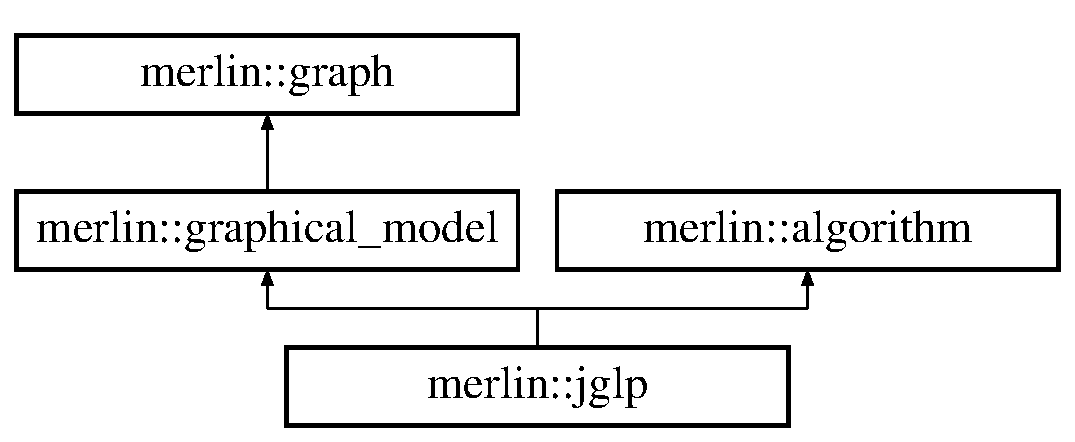
\includegraphics[height=3.000000cm]{classmerlin_1_1jglp}
\end{center}
\end{figure}
\subsection*{Classes}
\begin{DoxyCompactItemize}
\item 
struct \hyperlink{structmerlin_1_1jglp_1_1sPair}{s\+Pair}
\begin{DoxyCompactList}\small\item\em Helper class for pairs of sorted indices. \end{DoxyCompactList}\end{DoxyCompactItemize}
\subsection*{Public Types}
\begin{DoxyCompactItemize}
\item 
typedef \hyperlink{classmerlin_1_1graphical__model_ab2b46f09d8142bb68f243ecadbdabb6b}{graphical\+\_\+model\+::findex} \hyperlink{classmerlin_1_1jglp_ad5dee448584a712e94f82a9e6c9c071a}{findex}\hypertarget{classmerlin_1_1jglp_ad5dee448584a712e94f82a9e6c9c071a}{}\label{classmerlin_1_1jglp_ad5dee448584a712e94f82a9e6c9c071a}

\begin{DoxyCompactList}\small\item\em Factor index. \end{DoxyCompactList}\item 
typedef \hyperlink{classmerlin_1_1graphical__model_a275006a490bc09239c12a4d93d53b135}{graphical\+\_\+model\+::vindex} \hyperlink{classmerlin_1_1jglp_a85f09fc4dc206dd719f08d08b1db9591}{vindex}\hypertarget{classmerlin_1_1jglp_a85f09fc4dc206dd719f08d08b1db9591}{}\label{classmerlin_1_1jglp_a85f09fc4dc206dd719f08d08b1db9591}

\begin{DoxyCompactList}\small\item\em Variable index. \end{DoxyCompactList}\item 
typedef \hyperlink{classmerlin_1_1graphical__model_a615e25ec6594615fddfd4c3c4776b99f}{graphical\+\_\+model\+::flist} \hyperlink{classmerlin_1_1jglp_aae20606ec1b315bded44b64b5969fc2b}{flist}\hypertarget{classmerlin_1_1jglp_aae20606ec1b315bded44b64b5969fc2b}{}\label{classmerlin_1_1jglp_aae20606ec1b315bded44b64b5969fc2b}

\begin{DoxyCompactList}\small\item\em Collection of factor indices. \end{DoxyCompactList}\item 
typedef flist\+::const\+\_\+iterator \hyperlink{classmerlin_1_1jglp_aa30342c2a9795862a885bf62b6ac1293}{flist\+It}\hypertarget{classmerlin_1_1jglp_aa30342c2a9795862a885bf62b6ac1293}{}\label{classmerlin_1_1jglp_aa30342c2a9795862a885bf62b6ac1293}

\begin{DoxyCompactList}\small\item\em Iterator for collection of factor indeces. \end{DoxyCompactList}\end{DoxyCompactItemize}
\subsection*{Public Member Functions}
\begin{DoxyCompactItemize}
\item 
\hyperlink{classmerlin_1_1jglp_aa6fa80d5245138810714337e621567f7}{jglp} ()\hypertarget{classmerlin_1_1jglp_aa6fa80d5245138810714337e621567f7}{}\label{classmerlin_1_1jglp_aa6fa80d5245138810714337e621567f7}

\begin{DoxyCompactList}\small\item\em Default constructor. \end{DoxyCompactList}\item 
\hyperlink{classmerlin_1_1jglp_ad3b225e0288d9a911a5e8badcbc53e73}{jglp} (const \hyperlink{classmerlin_1_1graphical__model}{graphical\+\_\+model} \&gm)\hypertarget{classmerlin_1_1jglp_ad3b225e0288d9a911a5e8badcbc53e73}{}\label{classmerlin_1_1jglp_ad3b225e0288d9a911a5e8badcbc53e73}

\begin{DoxyCompactList}\small\item\em Constructor. \end{DoxyCompactList}\item 
virtual \hyperlink{classmerlin_1_1jglp}{jglp} $\ast$ \hyperlink{classmerlin_1_1jglp_af6e5931262caafec1aab81f6d3001419}{clone} () const 
\begin{DoxyCompactList}\small\item\em Clone the algorithm. \end{DoxyCompactList}\item 
double \hyperlink{classmerlin_1_1jglp_aeb00e60c9df427722f2ff791bdd056d9}{ub} () const 
\begin{DoxyCompactList}\small\item\em Upper bound on the optimal value. \end{DoxyCompactList}\item 
double \hyperlink{classmerlin_1_1jglp_a56a4aa254f07ee4a651bf343ee14d63b}{lb} () const 
\begin{DoxyCompactList}\small\item\em Lower bound on the optimal value. \end{DoxyCompactList}\item 
std\+::vector$<$ \hyperlink{classmerlin_1_1graph_a5cade38832f47248573e921276f122d6}{index} $>$ \hyperlink{classmerlin_1_1jglp_a4e7ff17be5074ce9010fda0154f81fbf}{best\+\_\+config} () const 
\begin{DoxyCompactList}\small\item\em Best configuration. \end{DoxyCompactList}\item 
double \hyperlink{classmerlin_1_1jglp_a2a6a565403cbddd77109a3a6f85e3d35}{logZ} () const 
\begin{DoxyCompactList}\small\item\em Log value of the partition function. \end{DoxyCompactList}\item 
double \hyperlink{classmerlin_1_1jglp_a6f964c4acb649a3bf24bd46e8c414113}{log\+Zub} () const 
\begin{DoxyCompactList}\small\item\em Upper bound on the log partition function. \end{DoxyCompactList}\item 
double \hyperlink{classmerlin_1_1jglp_a53e258c9ac8e80e2a99019f350fafe23}{log\+Zlb} () const 
\begin{DoxyCompactList}\small\item\em Lower bound on the log partition function. \end{DoxyCompactList}\item 
const \hyperlink{classmerlin_1_1factor}{factor} \& \hyperlink{classmerlin_1_1jglp_a75fe3423fa5f1d46f5878de99f732ed4}{belief} (size\+\_\+t f) const 
\begin{DoxyCompactList}\small\item\em Belief associated with a node of the graph. \end{DoxyCompactList}\item 
const \hyperlink{classmerlin_1_1factor}{factor} \& \hyperlink{classmerlin_1_1jglp_ab682129e900ebd41c44b0516e7997a9e}{belief} (\hyperlink{classmerlin_1_1variable}{variable} v) const 
\begin{DoxyCompactList}\small\item\em Belief associated with a particular variable. \end{DoxyCompactList}\item 
const \hyperlink{classmerlin_1_1factor}{factor} \& \hyperlink{classmerlin_1_1jglp_abc9393073179fadfd12999faea87a62c}{belief} (\hyperlink{classmerlin_1_1variable__set}{variable\+\_\+set} vs) const 
\begin{DoxyCompactList}\small\item\em Belief associated with a set of variables. \end{DoxyCompactList}\item 
const std\+::vector$<$ \hyperlink{classmerlin_1_1factor}{factor} $>$ \& \hyperlink{classmerlin_1_1jglp_a44be9483e6b79d87f70fd7c893d8f70a}{beliefs} () const 
\begin{DoxyCompactList}\small\item\em Beliefs associated with the variables. \end{DoxyCompactList}\item 
const \hyperlink{classmerlin_1_1graphical__model}{graphical\+\_\+model} \& \hyperlink{classmerlin_1_1jglp_adfca7a469dbd9a01486dca85af083b56}{get\+\_\+gm\+\_\+orig} () const \hypertarget{classmerlin_1_1jglp_adfca7a469dbd9a01486dca85af083b56}{}\label{classmerlin_1_1jglp_adfca7a469dbd9a01486dca85af083b56}

\begin{DoxyCompactList}\small\item\em Return the original graphical model. \end{DoxyCompactList}\item 
\hyperlink{classmerlin_1_1jglp_a7a0a5bdfdd803b351d9d86a86fd41029}{M\+E\+R\+\_\+\+E\+N\+UM} (Property, i\+Bound, Order, Iter, Debug)\hypertarget{classmerlin_1_1jglp_a7a0a5bdfdd803b351d9d86a86fd41029}{}\label{classmerlin_1_1jglp_a7a0a5bdfdd803b351d9d86a86fd41029}

\begin{DoxyCompactList}\small\item\em Properties of the algorithm. \end{DoxyCompactList}\item 
void \hyperlink{classmerlin_1_1jglp_a81a1ba0a30b0a415f95438b4e3b4979b}{set\+\_\+ibound} (size\+\_\+t i)
\begin{DoxyCompactList}\small\item\em Set the i-\/bound parameter. \end{DoxyCompactList}\item 
size\+\_\+t \hyperlink{classmerlin_1_1jglp_ab9b49439616ac5cc826dc3614d522ba8}{get\+\_\+ibound} () const \hypertarget{classmerlin_1_1jglp_ab9b49439616ac5cc826dc3614d522ba8}{}\label{classmerlin_1_1jglp_ab9b49439616ac5cc826dc3614d522ba8}

\begin{DoxyCompactList}\small\item\em Return the i-\/bound parameter. \end{DoxyCompactList}\item 
void \hyperlink{classmerlin_1_1jglp_ada0022232bd0e11e043d997341ebeb8c}{set\+\_\+order} (const variable\+\_\+order\+\_\+t \&ord)
\begin{DoxyCompactList}\small\item\em Set the variable elimination order. \end{DoxyCompactList}\item 
void \hyperlink{classmerlin_1_1jglp_a0cc988afd7be26d8e3abe557e87ca445}{set\+\_\+order\+\_\+method} (Order\+Method method)
\begin{DoxyCompactList}\small\item\em Set the variable elimination order method. \end{DoxyCompactList}\item 
const variable\+\_\+order\+\_\+t \& \hyperlink{classmerlin_1_1jglp_a03f29b87c291dc6c759c0ddef24569b8}{get\+\_\+order} ()\hypertarget{classmerlin_1_1jglp_a03f29b87c291dc6c759c0ddef24569b8}{}\label{classmerlin_1_1jglp_a03f29b87c291dc6c759c0ddef24569b8}

\begin{DoxyCompactList}\small\item\em Return the variable elimination order. \end{DoxyCompactList}\item 
const std\+::vector$<$ \hyperlink{classmerlin_1_1jglp_a85f09fc4dc206dd719f08d08b1db9591}{vindex} $>$ \& \hyperlink{classmerlin_1_1jglp_a3b2d6adcead0b1ec15ef9d0fbf412d1b}{get\+\_\+pseudo\+\_\+tree} ()\hypertarget{classmerlin_1_1jglp_a3b2d6adcead0b1ec15ef9d0fbf412d1b}{}\label{classmerlin_1_1jglp_a3b2d6adcead0b1ec15ef9d0fbf412d1b}

\begin{DoxyCompactList}\small\item\em Return the pseudo tree. \end{DoxyCompactList}\item 
void \hyperlink{classmerlin_1_1jglp_a652e12b270f52c59cf6a795847650d74}{set\+\_\+pseudo\+\_\+tree} (const std\+::vector$<$ \hyperlink{classmerlin_1_1jglp_a85f09fc4dc206dd719f08d08b1db9591}{vindex} $>$ \&p)
\begin{DoxyCompactList}\small\item\em Set the pseudo tree. \end{DoxyCompactList}\item 
void \hyperlink{classmerlin_1_1jglp_a788df051ff307d477af55bab2d671321}{set\+\_\+graphical\+\_\+model} (const \hyperlink{classmerlin_1_1graphical__model}{graphical\+\_\+model} \&gm)
\begin{DoxyCompactList}\small\item\em Set the graphical model content. \end{DoxyCompactList}\item 
void \hyperlink{classmerlin_1_1jglp_ae02d2c472b62bbbed8f06896c2688bdf}{set\+\_\+graphical\+\_\+model} (const std\+::vector$<$ \hyperlink{classmerlin_1_1factor}{factor} $>$ \&fs)
\begin{DoxyCompactList}\small\item\em Set the graphical model content from a list of factors. \end{DoxyCompactList}\item 
virtual void \hyperlink{classmerlin_1_1jglp_a5acb4097355e635727d2b9818351ec8c}{set\+\_\+properties} (std\+::string opt=std\+::string())
\begin{DoxyCompactList}\small\item\em Set the properties of the algorithm. \end{DoxyCompactList}\item 
\hyperlink{classmerlin_1_1factor}{factor} \hyperlink{classmerlin_1_1jglp_a99dba3581cf03ae19380974d294297e7}{elim} (const \hyperlink{classmerlin_1_1factor}{factor} \&F, const \hyperlink{classmerlin_1_1variable__set}{variable\+\_\+set} \&vs)
\begin{DoxyCompactList}\small\item\em Eliminate a set of variables from a factor. \end{DoxyCompactList}\item 
\hyperlink{classmerlin_1_1factor}{factor} \hyperlink{classmerlin_1_1jglp_a9a4ce84cb6de5b2b3dabc216d6738126}{marg} (const \hyperlink{classmerlin_1_1factor}{factor} \&F, const \hyperlink{classmerlin_1_1variable__set}{variable\+\_\+set} \&vs)
\begin{DoxyCompactList}\small\item\em Compute the marginal over a set of variables. \end{DoxyCompactList}\item 
double \hyperlink{classmerlin_1_1jglp_acd88ee331ca7257fcc0ee1d70c2fe24c}{score} (const std\+::vector$<$ \hyperlink{classmerlin_1_1factor}{factor} $>$ \&fin, const \hyperlink{classmerlin_1_1variable}{variable} \&VX, size\+\_\+t i, size\+\_\+t j)
\begin{DoxyCompactList}\small\item\em Scoring function for bucket aggregation. \end{DoxyCompactList}\item 
void \hyperlink{classmerlin_1_1jglp_a834f4f3ac58d3286843ed1e1fb8552dc}{init} ()\hypertarget{classmerlin_1_1jglp_a834f4f3ac58d3286843ed1e1fb8552dc}{}\label{classmerlin_1_1jglp_a834f4f3ac58d3286843ed1e1fb8552dc}

\begin{DoxyCompactList}\small\item\em Initialize the J\+G\+LP algorithm. \end{DoxyCompactList}\item 
void \hyperlink{classmerlin_1_1jglp_a8b61916d0cdfb09f2f45ab47d6c00872}{tighten} (size\+\_\+t n\+Iter, double stop\+Time=-\/1, double stop\+Obj=-\/1)
\begin{DoxyCompactList}\small\item\em Join graph propagation for tightening the bound. \end{DoxyCompactList}\item 
void \hyperlink{classmerlin_1_1jglp_a7f4e708a4dca8d3ae759a658e5f91f3b}{write\+\_\+solution} (const char $\ast$file\+\_\+name, const std\+::map$<$ size\+\_\+t, size\+\_\+t $>$ \&evidence, const std\+::map$<$ size\+\_\+t, size\+\_\+t $>$ \&old2new, const \hyperlink{classmerlin_1_1graphical__model}{graphical\+\_\+model} \&orig)
\begin{DoxyCompactList}\small\item\em Write the solution to the output file. \end{DoxyCompactList}\item 
void \hyperlink{classmerlin_1_1jglp_aa748730ca6abbe2359fb2497da674fb8}{run} ()
\begin{DoxyCompactList}\small\item\em Run the algorithm. \end{DoxyCompactList}\item 
std\+::vector$<$ \hyperlink{classmerlin_1_1graph_a5cade38832f47248573e921276f122d6}{index} $>$ \hyperlink{classmerlin_1_1jglp_af75558eff4ccc1ad72acc1af5af3cc79}{config} ()\hypertarget{classmerlin_1_1jglp_af75558eff4ccc1ad72acc1af5af3cc79}{}\label{classmerlin_1_1jglp_af75558eff4ccc1ad72acc1af5af3cc79}

\begin{DoxyCompactList}\small\item\em Return the M\+AP configuration following the propagation. \end{DoxyCompactList}\end{DoxyCompactItemize}
\subsection*{Protected Attributes}
\begin{DoxyCompactItemize}
\item 
\hyperlink{classmerlin_1_1graphical__model}{graphical\+\_\+model} \hyperlink{classmerlin_1_1jglp_ac0f668e6d434179145bfb10afce53938}{m\+\_\+gmo}\hypertarget{classmerlin_1_1jglp_ac0f668e6d434179145bfb10afce53938}{}\label{classmerlin_1_1jglp_ac0f668e6d434179145bfb10afce53938}

\begin{DoxyCompactList}\small\item\em Original graphical model. \end{DoxyCompactList}\item 
Order\+Method \hyperlink{classmerlin_1_1jglp_a406bdf7a6e931ff40a7c0a0ddcf8d099}{m\+\_\+order\+\_\+method}\hypertarget{classmerlin_1_1jglp_a406bdf7a6e931ff40a7c0a0ddcf8d099}{}\label{classmerlin_1_1jglp_a406bdf7a6e931ff40a7c0a0ddcf8d099}

\begin{DoxyCompactList}\small\item\em Variable ordering heuristic. \end{DoxyCompactList}\item 
size\+\_\+t \hyperlink{classmerlin_1_1jglp_a06d2c5e9d89c5af6e21ded02eaf3222b}{m\+\_\+ibound}\hypertarget{classmerlin_1_1jglp_a06d2c5e9d89c5af6e21ded02eaf3222b}{}\label{classmerlin_1_1jglp_a06d2c5e9d89c5af6e21ded02eaf3222b}

\begin{DoxyCompactList}\small\item\em Mini-\/bucket i-\/bound. \end{DoxyCompactList}\item 
double \hyperlink{classmerlin_1_1jglp_afb663294d5593789c47985869b36bd48}{m\+\_\+log\+\_\+z}\hypertarget{classmerlin_1_1jglp_afb663294d5593789c47985869b36bd48}{}\label{classmerlin_1_1jglp_afb663294d5593789c47985869b36bd48}

\begin{DoxyCompactList}\small\item\em Log partition function. \end{DoxyCompactList}\item 
double \hyperlink{classmerlin_1_1jglp_aa64d901abe0f4d02f144460323a386b4}{m\+\_\+lb}\hypertarget{classmerlin_1_1jglp_aa64d901abe0f4d02f144460323a386b4}{}\label{classmerlin_1_1jglp_aa64d901abe0f4d02f144460323a386b4}

\begin{DoxyCompactList}\small\item\em Lower bound. \end{DoxyCompactList}\item 
variable\+\_\+order\+\_\+t \hyperlink{classmerlin_1_1jglp_acb8107d4e410cd41509059edf21c254b}{m\+\_\+order}\hypertarget{classmerlin_1_1jglp_acb8107d4e410cd41509059edf21c254b}{}\label{classmerlin_1_1jglp_acb8107d4e410cd41509059edf21c254b}

\begin{DoxyCompactList}\small\item\em Elimination ordering. \end{DoxyCompactList}\item 
std\+::vector$<$ \hyperlink{classmerlin_1_1jglp_a85f09fc4dc206dd719f08d08b1db9591}{vindex} $>$ \hyperlink{classmerlin_1_1jglp_aa09f450dfa9c235b6257f44bc7b8cf09}{m\+\_\+parents}\hypertarget{classmerlin_1_1jglp_aa09f450dfa9c235b6257f44bc7b8cf09}{}\label{classmerlin_1_1jglp_aa09f450dfa9c235b6257f44bc7b8cf09}

\begin{DoxyCompactList}\small\item\em Pseudo tree. \end{DoxyCompactList}\item 
std\+::vector$<$ \hyperlink{classmerlin_1_1graph_a5cade38832f47248573e921276f122d6}{index} $>$ \hyperlink{classmerlin_1_1jglp_afc8a7b6244d60f4eeac42ad44e7c51f9}{m\+\_\+best\+\_\+config}\hypertarget{classmerlin_1_1jglp_afc8a7b6244d60f4eeac42ad44e7c51f9}{}\label{classmerlin_1_1jglp_afc8a7b6244d60f4eeac42ad44e7c51f9}

\begin{DoxyCompactList}\small\item\em M\+AP assignment. \end{DoxyCompactList}\item 
size\+\_\+t \hyperlink{classmerlin_1_1jglp_a7a526ba47d0647aa815c343bc82de239}{m\+\_\+num\+\_\+iter}\hypertarget{classmerlin_1_1jglp_a7a526ba47d0647aa815c343bc82de239}{}\label{classmerlin_1_1jglp_a7a526ba47d0647aa815c343bc82de239}

\begin{DoxyCompactList}\small\item\em Number of iterations. \end{DoxyCompactList}\item 
std\+::vector$<$ \hyperlink{classmerlin_1_1graphical__model_a615e25ec6594615fddfd4c3c4776b99f}{flist} $>$ \hyperlink{classmerlin_1_1jglp_abd8a4c838e9ff25444a8bb46e95a4fe3}{m\+\_\+mini\+\_\+buckets}\hypertarget{classmerlin_1_1jglp_abd8a4c838e9ff25444a8bb46e95a4fe3}{}\label{classmerlin_1_1jglp_abd8a4c838e9ff25444a8bb46e95a4fe3}

\begin{DoxyCompactList}\small\item\em Mini-\/buucket partitionings. \end{DoxyCompactList}\item 
bool \hyperlink{classmerlin_1_1jglp_a3747feeae5d36fa5568130d9d0519b24}{m\+\_\+debug}\hypertarget{classmerlin_1_1jglp_a3747feeae5d36fa5568130d9d0519b24}{}\label{classmerlin_1_1jglp_a3747feeae5d36fa5568130d9d0519b24}

\begin{DoxyCompactList}\small\item\em Internal debugging flag. \end{DoxyCompactList}\end{DoxyCompactItemize}
\subsection*{Additional Inherited Members}


\subsection{Detailed Description}
Join-\/\+Graph Linear Programming (ie, Weighted mini-\/buckets for M\+AP inference)

Tasks supported\+: M\+AP

J\+G\+LP is a specialization of the weighted mini-\/bucket algorithm to the M\+AP inference task. It builds a join graph by running the mini-\/bucket algorithm schemetically, and then it connects the mini-\/buckets residing in the same bucket. J\+G\+LP shifts costs along the edges of the join graph by matching the max marginals of any two clusters connected by an edge. In practice, the algorithm typically tightens the M\+AP upper bound, however this is not a guarantee. It keeps track of the tightest upper bound found and its corresponding assignment. 

Definition at line 50 of file jglp.\+h.



\subsection{Member Function Documentation}
\index{merlin\+::jglp@{merlin\+::jglp}!belief@{belief}}
\index{belief@{belief}!merlin\+::jglp@{merlin\+::jglp}}
\subsubsection[{\texorpdfstring{belief(size\+\_\+t f) const }{belief(size_t f) const }}]{\setlength{\rightskip}{0pt plus 5cm}const {\bf factor}\& merlin\+::jglp\+::belief (
\begin{DoxyParamCaption}
\item[{size\+\_\+t}]{i}
\end{DoxyParamCaption}
) const\hspace{0.3cm}{\ttfamily [inline]}, {\ttfamily [virtual]}}\hypertarget{classmerlin_1_1jglp_a75fe3423fa5f1d46f5878de99f732ed4}{}\label{classmerlin_1_1jglp_a75fe3423fa5f1d46f5878de99f732ed4}


Belief associated with a node of the graph. 

\begin{DoxyReturn}{Returns}
the belief associated with a node of the graph. Nodes correspond typically to variables. The belied is a function represented by the Factor class. 
\end{DoxyReturn}

\begin{DoxyParams}{Parameters}
{\em i} & The index of the node in the graph (from 0) \\
\hline
\end{DoxyParams}


Implements \hyperlink{classmerlin_1_1algorithm_a617b3e562037a7716f7cfd6cf1e55c19}{merlin\+::algorithm}.



Definition at line 105 of file jglp.\+h.

\index{merlin\+::jglp@{merlin\+::jglp}!belief@{belief}}
\index{belief@{belief}!merlin\+::jglp@{merlin\+::jglp}}
\subsubsection[{\texorpdfstring{belief(variable v) const }{belief(variable v) const }}]{\setlength{\rightskip}{0pt plus 5cm}const {\bf factor}\& merlin\+::jglp\+::belief (
\begin{DoxyParamCaption}
\item[{{\bf variable}}]{v}
\end{DoxyParamCaption}
) const\hspace{0.3cm}{\ttfamily [inline]}, {\ttfamily [virtual]}}\hypertarget{classmerlin_1_1jglp_ab682129e900ebd41c44b0516e7997a9e}{}\label{classmerlin_1_1jglp_ab682129e900ebd41c44b0516e7997a9e}


Belief associated with a particular variable. 


\begin{DoxyParams}{Parameters}
{\em v} & The variable to compute the belief of \\
\hline
\end{DoxyParams}
\begin{DoxyReturn}{Returns}
the belief associated with a particular variable in the graphical model. The belief is a function represented by the Factor class. 
\end{DoxyReturn}


Implements \hyperlink{classmerlin_1_1algorithm_adc966d1ed7ac479754441bab138f7efa}{merlin\+::algorithm}.



Definition at line 109 of file jglp.\+h.

\index{merlin\+::jglp@{merlin\+::jglp}!belief@{belief}}
\index{belief@{belief}!merlin\+::jglp@{merlin\+::jglp}}
\subsubsection[{\texorpdfstring{belief(variable\+\_\+set vs) const }{belief(variable_set vs) const }}]{\setlength{\rightskip}{0pt plus 5cm}const {\bf factor}\& merlin\+::jglp\+::belief (
\begin{DoxyParamCaption}
\item[{{\bf variable\+\_\+set}}]{vs}
\end{DoxyParamCaption}
) const\hspace{0.3cm}{\ttfamily [inline]}, {\ttfamily [virtual]}}\hypertarget{classmerlin_1_1jglp_abc9393073179fadfd12999faea87a62c}{}\label{classmerlin_1_1jglp_abc9393073179fadfd12999faea87a62c}


Belief associated with a set of variables. 


\begin{DoxyParams}{Parameters}
{\em vs} & The set of variables to compute the belief of \\
\hline
\end{DoxyParams}
\begin{DoxyReturn}{Returns}
the belief associated with a set of variables in the graphical model. The belief is a function represented by the Factor class. 
\end{DoxyReturn}


Implements \hyperlink{classmerlin_1_1algorithm_ad19b068623b85ad1cd4bb262e7bcfc6f}{merlin\+::algorithm}.



Definition at line 113 of file jglp.\+h.

\index{merlin\+::jglp@{merlin\+::jglp}!beliefs@{beliefs}}
\index{beliefs@{beliefs}!merlin\+::jglp@{merlin\+::jglp}}
\subsubsection[{\texorpdfstring{beliefs() const }{beliefs() const }}]{\setlength{\rightskip}{0pt plus 5cm}const std\+::vector$<${\bf factor}$>$\& merlin\+::jglp\+::beliefs (
\begin{DoxyParamCaption}
{}
\end{DoxyParamCaption}
) const\hspace{0.3cm}{\ttfamily [inline]}, {\ttfamily [virtual]}}\hypertarget{classmerlin_1_1jglp_a44be9483e6b79d87f70fd7c893d8f70a}{}\label{classmerlin_1_1jglp_a44be9483e6b79d87f70fd7c893d8f70a}


Beliefs associated with the variables. 

\begin{DoxyReturn}{Returns}
the beliefs associated with the variables in the graphical model (one belief for each of the variables). The output vector is indexed by the same indexes used for the variables. 
\end{DoxyReturn}


Implements \hyperlink{classmerlin_1_1algorithm_a0b70d8fe87b32bca601a3d116b673b47}{merlin\+::algorithm}.



Definition at line 117 of file jglp.\+h.

\index{merlin\+::jglp@{merlin\+::jglp}!best\+\_\+config@{best\+\_\+config}}
\index{best\+\_\+config@{best\+\_\+config}!merlin\+::jglp@{merlin\+::jglp}}
\subsubsection[{\texorpdfstring{best\+\_\+config() const }{best_config() const }}]{\setlength{\rightskip}{0pt plus 5cm}std\+::vector$<${\bf index}$>$ merlin\+::jglp\+::best\+\_\+config (
\begin{DoxyParamCaption}
{}
\end{DoxyParamCaption}
) const\hspace{0.3cm}{\ttfamily [inline]}, {\ttfamily [virtual]}}\hypertarget{classmerlin_1_1jglp_a4e7ff17be5074ce9010fda0154f81fbf}{}\label{classmerlin_1_1jglp_a4e7ff17be5074ce9010fda0154f81fbf}


Best configuration. 

\begin{DoxyReturn}{Returns}
a vector containing the best configuration of the variables (i.\+e., variable value assignments) found so far. It is specific to optimization tasks (e.\+g., M\+AP, Marginal M\+AP). 
\end{DoxyReturn}


Implements \hyperlink{classmerlin_1_1algorithm_a3d84d2595e6235db93a9bb3e1a012e48}{merlin\+::algorithm}.



Definition at line 91 of file jglp.\+h.



References m\+\_\+best\+\_\+config.

\index{merlin\+::jglp@{merlin\+::jglp}!clone@{clone}}
\index{clone@{clone}!merlin\+::jglp@{merlin\+::jglp}}
\subsubsection[{\texorpdfstring{clone() const }{clone() const }}]{\setlength{\rightskip}{0pt plus 5cm}virtual {\bf jglp}$\ast$ merlin\+::jglp\+::clone (
\begin{DoxyParamCaption}
{}
\end{DoxyParamCaption}
) const\hspace{0.3cm}{\ttfamily [inline]}, {\ttfamily [virtual]}}\hypertarget{classmerlin_1_1jglp_af6e5931262caafec1aab81f6d3001419}{}\label{classmerlin_1_1jglp_af6e5931262caafec1aab81f6d3001419}


Clone the algorithm. 

\begin{DoxyReturn}{Returns}
the pointer to the object containing the cloned algorithm. 
\end{DoxyReturn}


Implements \hyperlink{classmerlin_1_1algorithm_a10f787e24c1fd5ec92c26b18efb0b8db}{merlin\+::algorithm}.



Definition at line 80 of file jglp.\+h.



References jglp().

\index{merlin\+::jglp@{merlin\+::jglp}!elim@{elim}}
\index{elim@{elim}!merlin\+::jglp@{merlin\+::jglp}}
\subsubsection[{\texorpdfstring{elim(const factor \&\+F, const variable\+\_\+set \&vs)}{elim(const factor &F, const variable_set &vs)}}]{\setlength{\rightskip}{0pt plus 5cm}{\bf factor} merlin\+::jglp\+::elim (
\begin{DoxyParamCaption}
\item[{const {\bf factor} \&}]{F, }
\item[{const {\bf variable\+\_\+set} \&}]{vs}
\end{DoxyParamCaption}
)\hspace{0.3cm}{\ttfamily [inline]}}\hypertarget{classmerlin_1_1jglp_a99dba3581cf03ae19380974d294297e7}{}\label{classmerlin_1_1jglp_a99dba3581cf03ae19380974d294297e7}


Eliminate a set of variables from a factor. 


\begin{DoxyParams}{Parameters}
{\em F} & The reference of the factor to eliminate from \\
\hline
{\em vs} & The set of variables to be eliminated \\
\hline
\end{DoxyParams}
\begin{DoxyReturn}{Returns}
the factor resulted from eliminating the set of variables. 
\end{DoxyReturn}


Definition at line 262 of file jglp.\+h.



References merlin\+::factor\+::max().



Referenced by run().

\index{merlin\+::jglp@{merlin\+::jglp}!lb@{lb}}
\index{lb@{lb}!merlin\+::jglp@{merlin\+::jglp}}
\subsubsection[{\texorpdfstring{lb() const }{lb() const }}]{\setlength{\rightskip}{0pt plus 5cm}double merlin\+::jglp\+::lb (
\begin{DoxyParamCaption}
{}
\end{DoxyParamCaption}
) const\hspace{0.3cm}{\ttfamily [inline]}, {\ttfamily [virtual]}}\hypertarget{classmerlin_1_1jglp_a56a4aa254f07ee4a651bf343ee14d63b}{}\label{classmerlin_1_1jglp_a56a4aa254f07ee4a651bf343ee14d63b}


Lower bound on the optimal value. 

\begin{DoxyReturn}{Returns}
a lower bound on the optimal value defined by the inference task if available. 
\end{DoxyReturn}


Implements \hyperlink{classmerlin_1_1algorithm_adc3f19055c0466682b5577049df14863}{merlin\+::algorithm}.



Definition at line 88 of file jglp.\+h.



References m\+\_\+lb.

\index{merlin\+::jglp@{merlin\+::jglp}!logZ@{logZ}}
\index{logZ@{logZ}!merlin\+::jglp@{merlin\+::jglp}}
\subsubsection[{\texorpdfstring{log\+Z() const }{logZ() const }}]{\setlength{\rightskip}{0pt plus 5cm}double merlin\+::jglp\+::logZ (
\begin{DoxyParamCaption}
{}
\end{DoxyParamCaption}
) const\hspace{0.3cm}{\ttfamily [inline]}, {\ttfamily [virtual]}}\hypertarget{classmerlin_1_1jglp_a2a6a565403cbddd77109a3a6f85e3d35}{}\label{classmerlin_1_1jglp_a2a6a565403cbddd77109a3a6f85e3d35}


Log value of the partition function. 

\begin{DoxyReturn}{Returns}
an estimate the log parition function. If the inference algorithm is an exact one then the return value is the exact log value of the partition function. 
\end{DoxyReturn}


Implements \hyperlink{classmerlin_1_1algorithm_a26eadf71ba80c0a9cd3d7cfe18c95717}{merlin\+::algorithm}.



Definition at line 95 of file jglp.\+h.



References m\+\_\+log\+\_\+z.

\index{merlin\+::jglp@{merlin\+::jglp}!log\+Zlb@{log\+Zlb}}
\index{log\+Zlb@{log\+Zlb}!merlin\+::jglp@{merlin\+::jglp}}
\subsubsection[{\texorpdfstring{log\+Zlb() const }{logZlb() const }}]{\setlength{\rightskip}{0pt plus 5cm}double merlin\+::jglp\+::log\+Zlb (
\begin{DoxyParamCaption}
{}
\end{DoxyParamCaption}
) const\hspace{0.3cm}{\ttfamily [inline]}, {\ttfamily [virtual]}}\hypertarget{classmerlin_1_1jglp_a53e258c9ac8e80e2a99019f350fafe23}{}\label{classmerlin_1_1jglp_a53e258c9ac8e80e2a99019f350fafe23}


Lower bound on the log partition function. 

\begin{DoxyReturn}{Returns}
a lower bound on the log value of the parition function. 
\end{DoxyReturn}


Implements \hyperlink{classmerlin_1_1algorithm_a14d163a3e90a898487d3a6e273e1fecf}{merlin\+::algorithm}.



Definition at line 101 of file jglp.\+h.



References m\+\_\+log\+\_\+z.

\index{merlin\+::jglp@{merlin\+::jglp}!log\+Zub@{log\+Zub}}
\index{log\+Zub@{log\+Zub}!merlin\+::jglp@{merlin\+::jglp}}
\subsubsection[{\texorpdfstring{log\+Zub() const }{logZub() const }}]{\setlength{\rightskip}{0pt plus 5cm}double merlin\+::jglp\+::log\+Zub (
\begin{DoxyParamCaption}
{}
\end{DoxyParamCaption}
) const\hspace{0.3cm}{\ttfamily [inline]}, {\ttfamily [virtual]}}\hypertarget{classmerlin_1_1jglp_a6f964c4acb649a3bf24bd46e8c414113}{}\label{classmerlin_1_1jglp_a6f964c4acb649a3bf24bd46e8c414113}


Upper bound on the log partition function. 

\begin{DoxyReturn}{Returns}
an upper bound on the log value of the parition function. Most inference algorithms implemented in merlin support upper bounds on the log partition function. 
\end{DoxyReturn}


Implements \hyperlink{classmerlin_1_1algorithm_aeece2e8f008bcc94697353088c4afefe}{merlin\+::algorithm}.



Definition at line 98 of file jglp.\+h.



References m\+\_\+log\+\_\+z.

\index{merlin\+::jglp@{merlin\+::jglp}!marg@{marg}}
\index{marg@{marg}!merlin\+::jglp@{merlin\+::jglp}}
\subsubsection[{\texorpdfstring{marg(const factor \&\+F, const variable\+\_\+set \&vs)}{marg(const factor &F, const variable_set &vs)}}]{\setlength{\rightskip}{0pt plus 5cm}{\bf factor} merlin\+::jglp\+::marg (
\begin{DoxyParamCaption}
\item[{const {\bf factor} \&}]{F, }
\item[{const {\bf variable\+\_\+set} \&}]{vs}
\end{DoxyParamCaption}
)\hspace{0.3cm}{\ttfamily [inline]}}\hypertarget{classmerlin_1_1jglp_a9a4ce84cb6de5b2b3dabc216d6738126}{}\label{classmerlin_1_1jglp_a9a4ce84cb6de5b2b3dabc216d6738126}


Compute the marginal over a set of variables. 


\begin{DoxyParams}{Parameters}
{\em F} & The reference of the factor to marginalize over \\
\hline
{\em vs} & The set of variables representing the scope of the marginal \\
\hline
\end{DoxyParams}
\begin{DoxyReturn}{Returns}
the factor representing the marginal over the set of variables. 
\end{DoxyReturn}


Definition at line 272 of file jglp.\+h.



References merlin\+::factor\+::maxmarginal().



Referenced by run().

\index{merlin\+::jglp@{merlin\+::jglp}!run@{run}}
\index{run@{run}!merlin\+::jglp@{merlin\+::jglp}}
\subsubsection[{\texorpdfstring{run()}{run()}}]{\setlength{\rightskip}{0pt plus 5cm}void merlin\+::jglp\+::run (
\begin{DoxyParamCaption}
{}
\end{DoxyParamCaption}
)\hspace{0.3cm}{\ttfamily [inline]}, {\ttfamily [virtual]}}\hypertarget{classmerlin_1_1jglp_aa748730ca6abbe2359fb2497da674fb8}{}\label{classmerlin_1_1jglp_aa748730ca6abbe2359fb2497da674fb8}


Run the algorithm. 

Solves a probabilistic inference task. end for\+: variable elim order 

Implements \hyperlink{classmerlin_1_1algorithm_a6a701ee51b3d1009041702129161b0de}{merlin\+::algorithm}.



Definition at line 470 of file jglp.\+h.



References merlin\+::graph\+::add\+\_\+edge(), merlin\+::graphical\+\_\+model\+::add\+\_\+factor(), merlin\+::set$<$ T $>$\+::begin(), elim(), merlin\+::set$<$ T $>$\+::end(), merlin\+::factor\+::exp(), merlin\+::graphical\+\_\+model\+::get\+\_\+factors(), init(), merlin\+::graphical\+\_\+model\+::insert(), merlin\+::factor\+::log(), merlin\+::graphical\+\_\+model\+::log\+P(), merlin\+::graphical\+\_\+model\+::m\+\_\+factors, marg(), merlin\+::factor\+::max(), M\+E\+R\+L\+I\+N\+\_\+\+D\+O\+U\+B\+L\+E\+\_\+\+P\+R\+E\+C\+I\+S\+I\+ON, merlin\+::graphical\+\_\+model\+::num\+\_\+factors(), merlin\+::factor\+::nvar(), merlin\+::graphical\+\_\+model\+::nvar(), merlin\+::set$<$ T $>$\+::size(), tighten(), merlin\+::graphical\+\_\+model\+::var(), and merlin\+::graphical\+\_\+model\+::with\+\_\+variable().



Referenced by Merlin\+::run().

\index{merlin\+::jglp@{merlin\+::jglp}!score@{score}}
\index{score@{score}!merlin\+::jglp@{merlin\+::jglp}}
\subsubsection[{\texorpdfstring{score(const std\+::vector$<$ factor $>$ \&fin, const variable \&\+V\+X, size\+\_\+t i, size\+\_\+t j)}{score(const std::vector< factor > &fin, const variable &VX, size_t i, size_t j)}}]{\setlength{\rightskip}{0pt plus 5cm}double merlin\+::jglp\+::score (
\begin{DoxyParamCaption}
\item[{const std\+::vector$<$ {\bf factor} $>$ \&}]{fin, }
\item[{const {\bf variable} \&}]{VX, }
\item[{size\+\_\+t}]{i, }
\item[{size\+\_\+t}]{j}
\end{DoxyParamCaption}
)\hspace{0.3cm}{\ttfamily [inline]}}\hypertarget{classmerlin_1_1jglp_acd88ee331ca7257fcc0ee1d70c2fe24c}{}\label{classmerlin_1_1jglp_acd88ee331ca7257fcc0ee1d70c2fe24c}


Scoring function for bucket aggregation. 


\begin{DoxyParams}{Parameters}
{\em fin} & The set of factor scopes containing the pair (i,j) to be aggregated \\
\hline
{\em VX} & The bucket variable \\
\hline
{\em i} & The index of first scope \\
\hline
{\em j} & The index of the second pair \\
\hline
\end{DoxyParams}
\begin{DoxyReturn}{Returns}
the score that corresponds to aggregating the two scopes. It returns -\/3 if unable to combine, -\/1 for scope only aggregation, and otherwise a positive double score. 
\end{DoxyReturn}


Definition at line 287 of file jglp.\+h.



References merlin\+::factor\+::nvar(), and merlin\+::factor\+::vars().



Referenced by config().

\index{merlin\+::jglp@{merlin\+::jglp}!set\+\_\+graphical\+\_\+model@{set\+\_\+graphical\+\_\+model}}
\index{set\+\_\+graphical\+\_\+model@{set\+\_\+graphical\+\_\+model}!merlin\+::jglp@{merlin\+::jglp}}
\subsubsection[{\texorpdfstring{set\+\_\+graphical\+\_\+model(const graphical\+\_\+model \&gm)}{set_graphical_model(const graphical_model &gm)}}]{\setlength{\rightskip}{0pt plus 5cm}void merlin\+::jglp\+::set\+\_\+graphical\+\_\+model (
\begin{DoxyParamCaption}
\item[{const {\bf graphical\+\_\+model} \&}]{gm}
\end{DoxyParamCaption}
)\hspace{0.3cm}{\ttfamily [inline]}}\hypertarget{classmerlin_1_1jglp_a788df051ff307d477af55bab2d671321}{}\label{classmerlin_1_1jglp_a788df051ff307d477af55bab2d671321}


Set the graphical model content. 


\begin{DoxyParams}{Parameters}
{\em gm} & The reference to the graphical model object \\
\hline
\end{DoxyParams}


Definition at line 210 of file jglp.\+h.

\index{merlin\+::jglp@{merlin\+::jglp}!set\+\_\+graphical\+\_\+model@{set\+\_\+graphical\+\_\+model}}
\index{set\+\_\+graphical\+\_\+model@{set\+\_\+graphical\+\_\+model}!merlin\+::jglp@{merlin\+::jglp}}
\subsubsection[{\texorpdfstring{set\+\_\+graphical\+\_\+model(const std\+::vector$<$ factor $>$ \&fs)}{set_graphical_model(const std::vector< factor > &fs)}}]{\setlength{\rightskip}{0pt plus 5cm}void merlin\+::jglp\+::set\+\_\+graphical\+\_\+model (
\begin{DoxyParamCaption}
\item[{const std\+::vector$<$ {\bf factor} $>$ \&}]{fs}
\end{DoxyParamCaption}
)\hspace{0.3cm}{\ttfamily [inline]}}\hypertarget{classmerlin_1_1jglp_ae02d2c472b62bbbed8f06896c2688bdf}{}\label{classmerlin_1_1jglp_ae02d2c472b62bbbed8f06896c2688bdf}


Set the graphical model content from a list of factors. 


\begin{DoxyParams}{Parameters}
{\em fs} & The list of factors \\
\hline
\end{DoxyParams}


Definition at line 218 of file jglp.\+h.



References merlin\+::graphical\+\_\+model\+::graphical\+\_\+model().

\index{merlin\+::jglp@{merlin\+::jglp}!set\+\_\+ibound@{set\+\_\+ibound}}
\index{set\+\_\+ibound@{set\+\_\+ibound}!merlin\+::jglp@{merlin\+::jglp}}
\subsubsection[{\texorpdfstring{set\+\_\+ibound(size\+\_\+t i)}{set_ibound(size_t i)}}]{\setlength{\rightskip}{0pt plus 5cm}void merlin\+::jglp\+::set\+\_\+ibound (
\begin{DoxyParamCaption}
\item[{size\+\_\+t}]{i}
\end{DoxyParamCaption}
)\hspace{0.3cm}{\ttfamily [inline]}}\hypertarget{classmerlin_1_1jglp_a81a1ba0a30b0a415f95438b4e3b4979b}{}\label{classmerlin_1_1jglp_a81a1ba0a30b0a415f95438b4e3b4979b}


Set the i-\/bound parameter. 


\begin{DoxyParams}{Parameters}
{\em i} & The value of the i-\/bound ($>$ 1) \\
\hline
\end{DoxyParams}


Definition at line 156 of file jglp.\+h.



Referenced by set\+\_\+properties().

\index{merlin\+::jglp@{merlin\+::jglp}!set\+\_\+order@{set\+\_\+order}}
\index{set\+\_\+order@{set\+\_\+order}!merlin\+::jglp@{merlin\+::jglp}}
\subsubsection[{\texorpdfstring{set\+\_\+order(const variable\+\_\+order\+\_\+t \&ord)}{set_order(const variable_order_t &ord)}}]{\setlength{\rightskip}{0pt plus 5cm}void merlin\+::jglp\+::set\+\_\+order (
\begin{DoxyParamCaption}
\item[{const variable\+\_\+order\+\_\+t \&}]{ord}
\end{DoxyParamCaption}
)\hspace{0.3cm}{\ttfamily [inline]}}\hypertarget{classmerlin_1_1jglp_ada0022232bd0e11e043d997341ebeb8c}{}\label{classmerlin_1_1jglp_ada0022232bd0e11e043d997341ebeb8c}


Set the variable elimination order. 


\begin{DoxyParams}{Parameters}
{\em ord} & The variable order \\
\hline
\end{DoxyParams}


Definition at line 171 of file jglp.\+h.

\index{merlin\+::jglp@{merlin\+::jglp}!set\+\_\+order\+\_\+method@{set\+\_\+order\+\_\+method}}
\index{set\+\_\+order\+\_\+method@{set\+\_\+order\+\_\+method}!merlin\+::jglp@{merlin\+::jglp}}
\subsubsection[{\texorpdfstring{set\+\_\+order\+\_\+method(\+Order\+Method method)}{set_order_method(OrderMethod method)}}]{\setlength{\rightskip}{0pt plus 5cm}void merlin\+::jglp\+::set\+\_\+order\+\_\+method (
\begin{DoxyParamCaption}
\item[{Order\+Method}]{method}
\end{DoxyParamCaption}
)\hspace{0.3cm}{\ttfamily [inline]}}\hypertarget{classmerlin_1_1jglp_a0cc988afd7be26d8e3abe557e87ca445}{}\label{classmerlin_1_1jglp_a0cc988afd7be26d8e3abe557e87ca445}


Set the variable elimination order method. 


\begin{DoxyParams}{Parameters}
{\em method} & The elimination order method \\
\hline
\end{DoxyParams}


Definition at line 179 of file jglp.\+h.

\index{merlin\+::jglp@{merlin\+::jglp}!set\+\_\+properties@{set\+\_\+properties}}
\index{set\+\_\+properties@{set\+\_\+properties}!merlin\+::jglp@{merlin\+::jglp}}
\subsubsection[{\texorpdfstring{set\+\_\+properties(std\+::string opt=std\+::string())}{set_properties(std::string opt=std::string())}}]{\setlength{\rightskip}{0pt plus 5cm}virtual void merlin\+::jglp\+::set\+\_\+properties (
\begin{DoxyParamCaption}
\item[{std\+::string}]{opt = {\ttfamily std\+:\+:string()}}
\end{DoxyParamCaption}
)\hspace{0.3cm}{\ttfamily [inline]}, {\ttfamily [virtual]}}\hypertarget{classmerlin_1_1jglp_a5acb4097355e635727d2b9818351ec8c}{}\label{classmerlin_1_1jglp_a5acb4097355e635727d2b9818351ec8c}


Set the properties of the algorithm. 


\begin{DoxyParams}{Parameters}
{\em opt} & The string containing comma separated property value pairs \\
\hline
\end{DoxyParams}


Definition at line 226 of file jglp.\+h.



References set\+\_\+ibound().



Referenced by jglp(), and Merlin\+::run().

\index{merlin\+::jglp@{merlin\+::jglp}!set\+\_\+pseudo\+\_\+tree@{set\+\_\+pseudo\+\_\+tree}}
\index{set\+\_\+pseudo\+\_\+tree@{set\+\_\+pseudo\+\_\+tree}!merlin\+::jglp@{merlin\+::jglp}}
\subsubsection[{\texorpdfstring{set\+\_\+pseudo\+\_\+tree(const std\+::vector$<$ vindex $>$ \&p)}{set_pseudo_tree(const std::vector< vindex > &p)}}]{\setlength{\rightskip}{0pt plus 5cm}void merlin\+::jglp\+::set\+\_\+pseudo\+\_\+tree (
\begin{DoxyParamCaption}
\item[{const std\+::vector$<$ {\bf vindex} $>$ \&}]{p}
\end{DoxyParamCaption}
)\hspace{0.3cm}{\ttfamily [inline]}}\hypertarget{classmerlin_1_1jglp_a652e12b270f52c59cf6a795847650d74}{}\label{classmerlin_1_1jglp_a652e12b270f52c59cf6a795847650d74}


Set the pseudo tree. 


\begin{DoxyParams}{Parameters}
{\em p} & The vector representing the pseudo tree \\
\hline
\end{DoxyParams}


Definition at line 202 of file jglp.\+h.

\index{merlin\+::jglp@{merlin\+::jglp}!tighten@{tighten}}
\index{tighten@{tighten}!merlin\+::jglp@{merlin\+::jglp}}
\subsubsection[{\texorpdfstring{tighten(size\+\_\+t n\+Iter, double stop\+Time=-\/1, double stop\+Obj=-\/1)}{tighten(size_t nIter, double stopTime=-1, double stopObj=-1)}}]{\setlength{\rightskip}{0pt plus 5cm}void merlin\+::jglp\+::tighten (
\begin{DoxyParamCaption}
\item[{size\+\_\+t}]{n\+Iter, }
\item[{double}]{stop\+Time = {\ttfamily -\/1}, }
\item[{double}]{stop\+Obj = {\ttfamily -\/1}}
\end{DoxyParamCaption}
)\hspace{0.3cm}{\ttfamily [inline]}}\hypertarget{classmerlin_1_1jglp_a8b61916d0cdfb09f2f45ab47d6c00872}{}\label{classmerlin_1_1jglp_a8b61916d0cdfb09f2f45ab47d6c00872}


Join graph propagation for tightening the bound. 


\begin{DoxyParams}{Parameters}
{\em n\+Iter} & The number of iterations \\
\hline
{\em stop\+Time} & The time limit \\
\hline
{\em stop\+Obj} & The difference between two successive objective values \\
\hline
\end{DoxyParams}


Definition at line 366 of file jglp.\+h.



References config(), merlin\+::graph\+::edges(), merlin\+::graphical\+\_\+model\+::m\+\_\+factors, m\+\_\+log\+\_\+z, merlin\+::algorithm\+::m\+\_\+start\+\_\+time, and merlin\+::graphical\+\_\+model\+::num\+\_\+factors().



Referenced by run().

\index{merlin\+::jglp@{merlin\+::jglp}!ub@{ub}}
\index{ub@{ub}!merlin\+::jglp@{merlin\+::jglp}}
\subsubsection[{\texorpdfstring{ub() const }{ub() const }}]{\setlength{\rightskip}{0pt plus 5cm}double merlin\+::jglp\+::ub (
\begin{DoxyParamCaption}
{}
\end{DoxyParamCaption}
) const\hspace{0.3cm}{\ttfamily [inline]}, {\ttfamily [virtual]}}\hypertarget{classmerlin_1_1jglp_aeb00e60c9df427722f2ff791bdd056d9}{}\label{classmerlin_1_1jglp_aeb00e60c9df427722f2ff791bdd056d9}


Upper bound on the optimal value. 

\begin{DoxyReturn}{Returns}
an upper bound on the optimal value defined by the inference task. It is specific to optimization tasks such as M\+AP and Marginal M\+AP inference. 
\end{DoxyReturn}


Implements \hyperlink{classmerlin_1_1algorithm_a2698bb69f5559889d4903a640f08cd66}{merlin\+::algorithm}.



Definition at line 85 of file jglp.\+h.



References m\+\_\+log\+\_\+z.

\index{merlin\+::jglp@{merlin\+::jglp}!write\+\_\+solution@{write\+\_\+solution}}
\index{write\+\_\+solution@{write\+\_\+solution}!merlin\+::jglp@{merlin\+::jglp}}
\subsubsection[{\texorpdfstring{write\+\_\+solution(const char $\ast$file\+\_\+name, const std\+::map$<$ size\+\_\+t, size\+\_\+t $>$ \&evidence, const std\+::map$<$ size\+\_\+t, size\+\_\+t $>$ \&old2new, const graphical\+\_\+model \&orig)}{write_solution(const char *file_name, const std::map< size_t, size_t > &evidence, const std::map< size_t, size_t > &old2new, const graphical_model &orig)}}]{\setlength{\rightskip}{0pt plus 5cm}void merlin\+::jglp\+::write\+\_\+solution (
\begin{DoxyParamCaption}
\item[{const char $\ast$}]{file\+\_\+name, }
\item[{const std\+::map$<$ size\+\_\+t, size\+\_\+t $>$ \&}]{evidence, }
\item[{const std\+::map$<$ size\+\_\+t, size\+\_\+t $>$ \&}]{old2new, }
\item[{const {\bf graphical\+\_\+model} \&}]{orig}
\end{DoxyParamCaption}
)\hspace{0.3cm}{\ttfamily [inline]}}\hypertarget{classmerlin_1_1jglp_a7f4e708a4dca8d3ae759a658e5f91f3b}{}\label{classmerlin_1_1jglp_a7f4e708a4dca8d3ae759a658e5f91f3b}


Write the solution to the output file. 


\begin{DoxyParams}{Parameters}
{\em filename} & The output file name \\
\hline
{\em evidence} & The evidence variable value pairs \\
\hline
{\em old2new} & The mapping between old and new variable indexing \\
\hline
{\em orig} & The graphical model prior to asserting evidence \\
\hline
\end{DoxyParams}


Definition at line 447 of file jglp.\+h.



References merlin\+::graphical\+\_\+model\+::nvar().



Referenced by Merlin\+::run().



The documentation for this class was generated from the following file\+:\begin{DoxyCompactItemize}
\item 
src/include/\hyperlink{jglp_8h}{jglp.\+h}\end{DoxyCompactItemize}

\hypertarget{classmerlin_1_1lbp}{}\section{merlin\+:\+:lbp Class Reference}
\label{classmerlin_1_1lbp}\index{merlin\+::lbp@{merlin\+::lbp}}


{\ttfamily \#include $<$lbp.\+h$>$}

Inheritance diagram for merlin\+:\+:lbp\+:\begin{figure}[H]
\begin{center}
\leavevmode
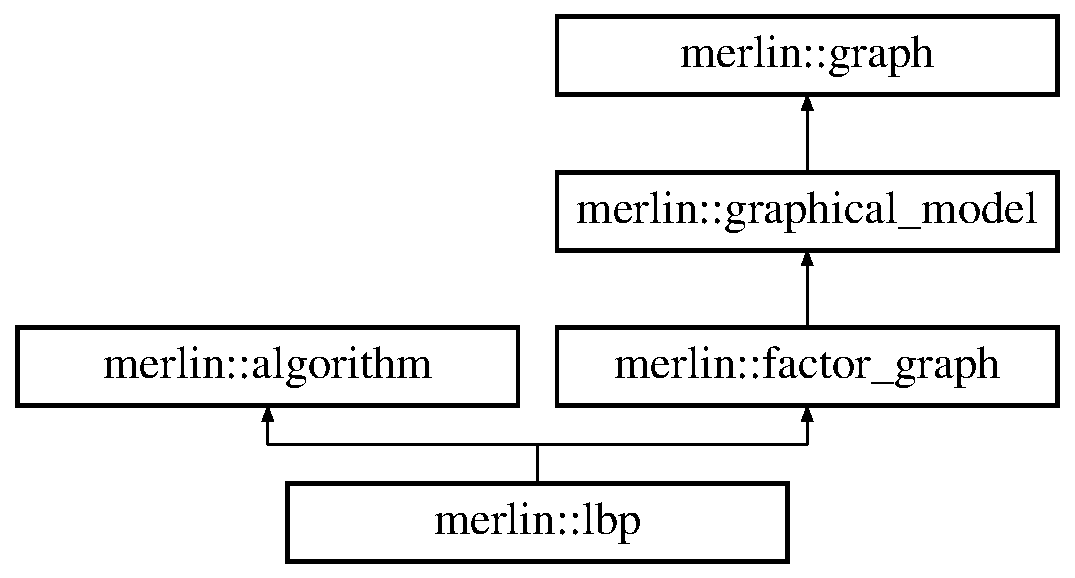
\includegraphics[height=4.000000cm]{classmerlin_1_1lbp}
\end{center}
\end{figure}
\subsection*{Public Types}
\begin{DoxyCompactItemize}
\item 
typedef \hyperlink{classmerlin_1_1factor__graph_a533556bd4ec6961b63a91a80a8a37508}{factor\+\_\+graph\+::findex} \hyperlink{classmerlin_1_1lbp_ad925905e6ca72cc3801260e7e63b7cae}{findex}\hypertarget{classmerlin_1_1lbp_ad925905e6ca72cc3801260e7e63b7cae}{}\label{classmerlin_1_1lbp_ad925905e6ca72cc3801260e7e63b7cae}

\begin{DoxyCompactList}\small\item\em Factor index. \end{DoxyCompactList}\item 
typedef \hyperlink{classmerlin_1_1factor__graph_a6b8a8220d86d6a6f91a8d2c7dd00ddc9}{factor\+\_\+graph\+::vindex} \hyperlink{classmerlin_1_1lbp_a2830aeb04ade80d6955b65297a59f68a}{vindex}\hypertarget{classmerlin_1_1lbp_a2830aeb04ade80d6955b65297a59f68a}{}\label{classmerlin_1_1lbp_a2830aeb04ade80d6955b65297a59f68a}

\begin{DoxyCompactList}\small\item\em Variable index. \end{DoxyCompactList}\item 
typedef \hyperlink{classmerlin_1_1factor__graph_a48dec4ea8a655315053984a81fe93ebc}{factor\+\_\+graph\+::flist} \hyperlink{classmerlin_1_1lbp_aefcbe2afa6efb09b12788e83cd7460f5}{flist}\hypertarget{classmerlin_1_1lbp_aefcbe2afa6efb09b12788e83cd7460f5}{}\label{classmerlin_1_1lbp_aefcbe2afa6efb09b12788e83cd7460f5}

\begin{DoxyCompactList}\small\item\em Collection of factor indices. \end{DoxyCompactList}\end{DoxyCompactItemize}
\subsection*{Public Member Functions}
\begin{DoxyCompactItemize}
\item 
\hyperlink{classmerlin_1_1lbp_aec902b835fbb159f872a9101cd007b7e}{lbp} ()\hypertarget{classmerlin_1_1lbp_aec902b835fbb159f872a9101cd007b7e}{}\label{classmerlin_1_1lbp_aec902b835fbb159f872a9101cd007b7e}

\begin{DoxyCompactList}\small\item\em Constructs algorithm instance over an empty factor graph. \end{DoxyCompactList}\item 
\hyperlink{classmerlin_1_1lbp_a46fbc09692ece741ba66da1a36b84fb3}{lbp} (const \hyperlink{classmerlin_1_1factor__graph}{factor\+\_\+graph} \&fg)
\begin{DoxyCompactList}\small\item\em Constructs algorithm instance from a copy of a factor graph. \end{DoxyCompactList}\item 
\hyperlink{classmerlin_1_1lbp_a5caa6f3d93015569031933bbce944aa4}{lbp} (std\+::vector$<$ \hyperlink{classmerlin_1_1factor}{factor} $>$ fs)
\begin{DoxyCompactList}\small\item\em Constructs algorithm instance from a list of factors. \end{DoxyCompactList}\item 
{\footnotesize template$<$class Input\+Iterator $>$ }\\\hyperlink{classmerlin_1_1lbp_ad4c9c7ba780848817d9f49e2e7537fb3}{lbp} (Input\+Iterator f, Input\+Iterator l)
\begin{DoxyCompactList}\small\item\em Constructs algorithm instance from input iterators. \end{DoxyCompactList}\item 
virtual \hyperlink{classmerlin_1_1lbp}{lbp} $\ast$ \hyperlink{classmerlin_1_1lbp_a4d2e317106a40ca49074f898a7a46fb0}{clone} () const 
\begin{DoxyCompactList}\small\item\em Clone the algorithm object. \end{DoxyCompactList}\item 
\hyperlink{classmerlin_1_1factor}{merlin\+::factor} \& \hyperlink{classmerlin_1_1lbp_a35585f32c077c507ed3582ee72d9e0d1}{bel} (size\+\_\+t f)\hypertarget{classmerlin_1_1lbp_a35585f32c077c507ed3582ee72d9e0d1}{}\label{classmerlin_1_1lbp_a35585f32c077c507ed3582ee72d9e0d1}

\begin{DoxyCompactList}\small\item\em Mutable accessor to a belief. \end{DoxyCompactList}\item 
const \hyperlink{classmerlin_1_1factor}{factor} \& \hyperlink{classmerlin_1_1lbp_a1df7d0dc71990b595c1a169498a2e087}{belief} (size\+\_\+t f) const 
\begin{DoxyCompactList}\small\item\em Belief associated with a node of the graph. \end{DoxyCompactList}\item 
const \hyperlink{classmerlin_1_1factor}{factor} \& \hyperlink{classmerlin_1_1lbp_af34aa24b4de8a0ae9f579ba6d83ee0bf}{belief} (\hyperlink{classmerlin_1_1variable}{variable} v) const 
\begin{DoxyCompactList}\small\item\em Belief associated with a particular variable. \end{DoxyCompactList}\item 
const \hyperlink{classmerlin_1_1factor}{factor} \& \hyperlink{classmerlin_1_1lbp_a37223c0f6db663160062bed87d2ac803}{belief} (\hyperlink{classmerlin_1_1variable__set}{variable\+\_\+set} vs) const 
\begin{DoxyCompactList}\small\item\em Belief associated with a set of variables. \end{DoxyCompactList}\item 
const std\+::vector$<$ \hyperlink{classmerlin_1_1factor}{factor} $>$ \& \hyperlink{classmerlin_1_1lbp_adccd484965707ae36ffc7f1d49b58ac9}{beliefs} () const 
\begin{DoxyCompactList}\small\item\em Beliefs associated with the variables. \end{DoxyCompactList}\item 
double \hyperlink{classmerlin_1_1lbp_af7cec119584c4ca671a82e23ac5098f1}{lb} () const 
\begin{DoxyCompactList}\small\item\em Lower bound on the optimal value. \end{DoxyCompactList}\item 
double \hyperlink{classmerlin_1_1lbp_a6f47094c1dd1b721c8b55b2a104bf708}{ub} () const 
\begin{DoxyCompactList}\small\item\em Upper bound on the optimal value. \end{DoxyCompactList}\item 
std\+::vector$<$ \hyperlink{classmerlin_1_1graph_a5cade38832f47248573e921276f122d6}{index} $>$ \hyperlink{classmerlin_1_1lbp_a7511d2d8fe99649f85a5c8ae88a8a379}{best\+\_\+config} () const 
\begin{DoxyCompactList}\small\item\em Best configuration. \end{DoxyCompactList}\item 
double \hyperlink{classmerlin_1_1lbp_a5f0f0d6b2605e1b3f47b6de9875d5590}{logZ} () const 
\begin{DoxyCompactList}\small\item\em Log value of the partition function. \end{DoxyCompactList}\item 
double \hyperlink{classmerlin_1_1lbp_a0451118b6fa2c1017512879e025afd4d}{log\+Zub} () const 
\begin{DoxyCompactList}\small\item\em Upper bound on the log partition function. \end{DoxyCompactList}\item 
double \hyperlink{classmerlin_1_1lbp_ada4dd7a71b8ac11ad419f3f7b1b6d658}{log\+Zlb} () const 
\begin{DoxyCompactList}\small\item\em Lower bound on the log partition function. \end{DoxyCompactList}\item 
\hyperlink{classmerlin_1_1lbp_ab4dc295e5265a3a2e259dc979ba35b91}{M\+E\+R\+\_\+\+E\+N\+UM} (Schedule, Fixed, Random, Flood, Priority)\hypertarget{classmerlin_1_1lbp_ab4dc295e5265a3a2e259dc979ba35b91}{}\label{classmerlin_1_1lbp_ab4dc295e5265a3a2e259dc979ba35b91}

\begin{DoxyCompactList}\small\item\em Types of propagation schedules. \end{DoxyCompactList}\item 
\hyperlink{classmerlin_1_1lbp_ad8d39f5967a07d53b7c27459a961bf66}{M\+E\+R\+\_\+\+E\+N\+UM} (Property, Schedule, Distance, Stop\+Iter, Stop\+Obj, Stop\+Msg, Debug)\hypertarget{classmerlin_1_1lbp_ad8d39f5967a07d53b7c27459a961bf66}{}\label{classmerlin_1_1lbp_ad8d39f5967a07d53b7c27459a961bf66}

\begin{DoxyCompactList}\small\item\em Properties of the algorithm. \end{DoxyCompactList}\item 
virtual void \hyperlink{classmerlin_1_1lbp_a2feb90924b5d7bf82a40bf93912041d0}{set\+\_\+properties} (std\+::string opt=std\+::string())
\begin{DoxyCompactList}\small\item\em Set the properties of the algorithm. \end{DoxyCompactList}\item 
void \hyperlink{classmerlin_1_1lbp_a61e6c00e8236acc65b59194e09180692}{init} ()\hypertarget{classmerlin_1_1lbp_a61e6c00e8236acc65b59194e09180692}{}\label{classmerlin_1_1lbp_a61e6c00e8236acc65b59194e09180692}

\begin{DoxyCompactList}\small\item\em Initialize the L\+BP algorithm. \end{DoxyCompactList}\item 
void \hyperlink{classmerlin_1_1lbp_ad6e56e73dd550f3580b4910536367a52}{write\+\_\+solution} (const char $\ast$file\+\_\+name, const std\+::map$<$ size\+\_\+t, size\+\_\+t $>$ \&evidence, const std\+::map$<$ size\+\_\+t, size\+\_\+t $>$ \&old2new, const \hyperlink{classmerlin_1_1graphical__model}{graphical\+\_\+model} \&orig)
\begin{DoxyCompactList}\small\item\em Write the solution to the output file. \end{DoxyCompactList}\item 
void \hyperlink{classmerlin_1_1lbp_afa31a31b0cfd63590d57cb453a6ab751}{run} ()
\begin{DoxyCompactList}\small\item\em Run the algorithm. \end{DoxyCompactList}\end{DoxyCompactItemize}
\subsection*{Protected Member Functions}
\begin{DoxyCompactItemize}
\item 
double \hyperlink{classmerlin_1_1lbp_a7970c64fc5ea704345d85bbdeda483ff}{obj\+\_\+entropy} (size\+\_\+t n)
\begin{DoxyCompactList}\small\item\em Entropy computation. \end{DoxyCompactList}\item 
void \hyperlink{classmerlin_1_1lbp_a48e9c7a9302829c21e6fd26f425e0237}{calc\+\_\+belief} (size\+\_\+t n)
\begin{DoxyCompactList}\small\item\em Belief computation. \end{DoxyCompactList}\item 
void \hyperlink{classmerlin_1_1lbp_a861d70a75592462bfe44aed5eda6407a}{accept\+\_\+incoming} (size\+\_\+t n)
\begin{DoxyCompactList}\small\item\em Incoming messages computation. \end{DoxyCompactList}\item 
void \hyperlink{classmerlin_1_1lbp_a05d07707c1eb9824c0e762ab0a3d80be}{update\+\_\+outgoing} (size\+\_\+t n)
\begin{DoxyCompactList}\small\item\em Outgoing (new) messages computation. \end{DoxyCompactList}\end{DoxyCompactItemize}
\subsection*{Protected Attributes}
\begin{DoxyCompactItemize}
\item 
std\+::vector$<$ \hyperlink{classmerlin_1_1factor}{factor} $>$ \hyperlink{classmerlin_1_1lbp_a866612087672e1b6a4a7bc24db71b8ea}{m\+\_\+beliefs}\hypertarget{classmerlin_1_1lbp_a866612087672e1b6a4a7bc24db71b8ea}{}\label{classmerlin_1_1lbp_a866612087672e1b6a4a7bc24db71b8ea}

\begin{DoxyCompactList}\small\item\em Store calculated messages and beliefs. \end{DoxyCompactList}\item 
std\+::vector$<$ \hyperlink{classmerlin_1_1factor}{factor} $>$ \hyperlink{classmerlin_1_1lbp_a36f83f09530a6d38000dd3e32c80c2b1}{m\+\_\+msg}\hypertarget{classmerlin_1_1lbp_a36f83f09530a6d38000dd3e32c80c2b1}{}\label{classmerlin_1_1lbp_a36f83f09530a6d38000dd3e32c80c2b1}

\begin{DoxyCompactList}\small\item\em Store messages. \end{DoxyCompactList}\item 
std\+::vector$<$ \hyperlink{classmerlin_1_1factor}{factor} $>$ \hyperlink{classmerlin_1_1lbp_acbcb875159cc0ba343201457db76c63c}{m\+\_\+msg\+\_\+new}\hypertarget{classmerlin_1_1lbp_acbcb875159cc0ba343201457db76c63c}{}\label{classmerlin_1_1lbp_acbcb875159cc0ba343201457db76c63c}

\begin{DoxyCompactList}\small\item\em Store new messages. \end{DoxyCompactList}\item 
\hyperlink{classmerlin_1_1indexed__heap}{indexed\+\_\+heap} \hyperlink{classmerlin_1_1lbp_afea235d05bdf4528aebcdbecfbdbd5f7}{m\+\_\+priority}\hypertarget{classmerlin_1_1lbp_afea235d05bdf4528aebcdbecfbdbd5f7}{}\label{classmerlin_1_1lbp_afea235d05bdf4528aebcdbecfbdbd5f7}

\begin{DoxyCompactList}\small\item\em Store m\+\_\+priority schedule of edges. \end{DoxyCompactList}\item 
std\+::vector$<$ \hyperlink{classmerlin_1_1lbp_ad925905e6ca72cc3801260e7e63b7cae}{findex} $>$ \hyperlink{classmerlin_1_1lbp_ab2ab30c257e4cc2683309852fad4b57a}{m\+\_\+forder}\hypertarget{classmerlin_1_1lbp_ab2ab30c257e4cc2683309852fad4b57a}{}\label{classmerlin_1_1lbp_ab2ab30c257e4cc2683309852fad4b57a}

\begin{DoxyCompactList}\small\item\em Fixed order of factors. \end{DoxyCompactList}\item 
Schedule \hyperlink{classmerlin_1_1lbp_a612e3dee4fede5efb97edf155c7d6d6f}{m\+\_\+sched}\hypertarget{classmerlin_1_1lbp_a612e3dee4fede5efb97edf155c7d6d6f}{}\label{classmerlin_1_1lbp_a612e3dee4fede5efb97edf155c7d6d6f}

\begin{DoxyCompactList}\small\item\em Schedule type. \end{DoxyCompactList}\item 
factor\+::\+Distance \hyperlink{classmerlin_1_1lbp_ad38eb15e14383af32cc33beed58d0a33}{m\+\_\+dist}\hypertarget{classmerlin_1_1lbp_ad38eb15e14383af32cc33beed58d0a33}{}\label{classmerlin_1_1lbp_ad38eb15e14383af32cc33beed58d0a33}

\begin{DoxyCompactList}\small\item\em Message distance measure for priority\+\_\+. \end{DoxyCompactList}\item 
double \hyperlink{classmerlin_1_1lbp_aae920e31f7765ddedd24326ad28dde15}{m\+\_\+log\+\_\+z}\hypertarget{classmerlin_1_1lbp_aae920e31f7765ddedd24326ad28dde15}{}\label{classmerlin_1_1lbp_aae920e31f7765ddedd24326ad28dde15}

\begin{DoxyCompactList}\small\item\em Current objective function value. \end{DoxyCompactList}\item 
bool \hyperlink{classmerlin_1_1lbp_a0f344f5422987ca3b2bd13cb5c3e5368}{m\+\_\+debug}\hypertarget{classmerlin_1_1lbp_a0f344f5422987ca3b2bd13cb5c3e5368}{}\label{classmerlin_1_1lbp_a0f344f5422987ca3b2bd13cb5c3e5368}

\begin{DoxyCompactList}\small\item\em Internal debugging flag. \end{DoxyCompactList}\end{DoxyCompactItemize}
\subsection*{Additional Inherited Members}


\subsection{Detailed Description}
Loopy belief propagation over the factor graph.

Tasks supported\+: M\+AR

L\+BP propagates the messages along a factor graph representation of the original graphical model. It also computes an estimate of the partition function (it doesn\textquotesingle{}t guarantee an upper or lower bound on Z). 

Definition at line 47 of file lbp.\+h.



\subsection{Constructor \& Destructor Documentation}
\index{merlin\+::lbp@{merlin\+::lbp}!lbp@{lbp}}
\index{lbp@{lbp}!merlin\+::lbp@{merlin\+::lbp}}
\subsubsection[{\texorpdfstring{lbp(const factor\+\_\+graph \&fg)}{lbp(const factor_graph &fg)}}]{\setlength{\rightskip}{0pt plus 5cm}merlin\+::lbp\+::lbp (
\begin{DoxyParamCaption}
\item[{const {\bf factor\+\_\+graph} \&}]{fg}
\end{DoxyParamCaption}
)\hspace{0.3cm}{\ttfamily [inline]}}\hypertarget{classmerlin_1_1lbp_a46fbc09692ece741ba66da1a36b84fb3}{}\label{classmerlin_1_1lbp_a46fbc09692ece741ba66da1a36b84fb3}


Constructs algorithm instance from a copy of a factor graph. 


\begin{DoxyParams}{Parameters}
{\em fg} & A factor graph \\
\hline
\end{DoxyParams}


Definition at line 67 of file lbp.\+h.



References set\+\_\+properties().

\index{merlin\+::lbp@{merlin\+::lbp}!lbp@{lbp}}
\index{lbp@{lbp}!merlin\+::lbp@{merlin\+::lbp}}
\subsubsection[{\texorpdfstring{lbp(std\+::vector$<$ factor $>$ fs)}{lbp(std::vector< factor > fs)}}]{\setlength{\rightskip}{0pt plus 5cm}merlin\+::lbp\+::lbp (
\begin{DoxyParamCaption}
\item[{std\+::vector$<$ {\bf factor} $>$}]{fs}
\end{DoxyParamCaption}
)\hspace{0.3cm}{\ttfamily [inline]}}\hypertarget{classmerlin_1_1lbp_a5caa6f3d93015569031933bbce944aa4}{}\label{classmerlin_1_1lbp_a5caa6f3d93015569031933bbce944aa4}


Constructs algorithm instance from a list of factors. 


\begin{DoxyParams}{Parameters}
{\em fs} & A list of factors \\
\hline
\end{DoxyParams}


Definition at line 75 of file lbp.\+h.



References set\+\_\+properties().

\index{merlin\+::lbp@{merlin\+::lbp}!lbp@{lbp}}
\index{lbp@{lbp}!merlin\+::lbp@{merlin\+::lbp}}
\subsubsection[{\texorpdfstring{lbp(\+Input\+Iterator f, Input\+Iterator l)}{lbp(InputIterator f, InputIterator l)}}]{\setlength{\rightskip}{0pt plus 5cm}template$<$class Input\+Iterator $>$ merlin\+::lbp\+::lbp (
\begin{DoxyParamCaption}
\item[{Input\+Iterator}]{f, }
\item[{Input\+Iterator}]{l}
\end{DoxyParamCaption}
)\hspace{0.3cm}{\ttfamily [inline]}}\hypertarget{classmerlin_1_1lbp_ad4c9c7ba780848817d9f49e2e7537fb3}{}\label{classmerlin_1_1lbp_ad4c9c7ba780848817d9f49e2e7537fb3}


Constructs algorithm instance from input iterators. 


\begin{DoxyParams}{Parameters}
{\em f} & An iterator to beginning \\
\hline
{\em l} & An iterator to end \\
\hline
\end{DoxyParams}


Definition at line 85 of file lbp.\+h.



References set\+\_\+properties().



\subsection{Member Function Documentation}
\index{merlin\+::lbp@{merlin\+::lbp}!accept\+\_\+incoming@{accept\+\_\+incoming}}
\index{accept\+\_\+incoming@{accept\+\_\+incoming}!merlin\+::lbp@{merlin\+::lbp}}
\subsubsection[{\texorpdfstring{accept\+\_\+incoming(size\+\_\+t n)}{accept_incoming(size_t n)}}]{\setlength{\rightskip}{0pt plus 5cm}void merlin\+::lbp\+::accept\+\_\+incoming (
\begin{DoxyParamCaption}
\item[{size\+\_\+t}]{n}
\end{DoxyParamCaption}
)\hspace{0.3cm}{\ttfamily [inline]}, {\ttfamily [protected]}}\hypertarget{classmerlin_1_1lbp_a861d70a75592462bfe44aed5eda6407a}{}\label{classmerlin_1_1lbp_a861d70a75592462bfe44aed5eda6407a}


Incoming messages computation. 

Accept all the incoming messages into a node, and recompute its belief. 
\begin{DoxyParams}{Parameters}
{\em n} & The index of the node \\
\hline
\end{DoxyParams}


Definition at line 476 of file lbp.\+h.



References merlin\+::set$<$ T $>$\+::begin(), bel(), merlin\+::set$<$ T $>$\+::end(), merlin\+::indexed\+\_\+heap\+::erase(), merlin\+::graphical\+\_\+model\+::get\+\_\+factor(), merlin\+::graph\+::neighbors(), and merlin\+::factor\+::sum().



Referenced by run().

\index{merlin\+::lbp@{merlin\+::lbp}!belief@{belief}}
\index{belief@{belief}!merlin\+::lbp@{merlin\+::lbp}}
\subsubsection[{\texorpdfstring{belief(size\+\_\+t f) const }{belief(size_t f) const }}]{\setlength{\rightskip}{0pt plus 5cm}const {\bf factor}\& merlin\+::lbp\+::belief (
\begin{DoxyParamCaption}
\item[{size\+\_\+t}]{i}
\end{DoxyParamCaption}
) const\hspace{0.3cm}{\ttfamily [inline]}, {\ttfamily [virtual]}}\hypertarget{classmerlin_1_1lbp_a1df7d0dc71990b595c1a169498a2e087}{}\label{classmerlin_1_1lbp_a1df7d0dc71990b595c1a169498a2e087}


Belief associated with a node of the graph. 

\begin{DoxyReturn}{Returns}
the belief associated with a node of the graph. Nodes correspond typically to variables. The belied is a function represented by the Factor class. 
\end{DoxyReturn}

\begin{DoxyParams}{Parameters}
{\em i} & The index of the node in the graph (from 0) \\
\hline
\end{DoxyParams}


Implements \hyperlink{classmerlin_1_1algorithm_a617b3e562037a7716f7cfd6cf1e55c19}{merlin\+::algorithm}.



Definition at line 105 of file lbp.\+h.



References m\+\_\+beliefs.



Referenced by belief(), obj\+\_\+entropy(), run(), update\+\_\+outgoing(), and write\+\_\+solution().

\index{merlin\+::lbp@{merlin\+::lbp}!belief@{belief}}
\index{belief@{belief}!merlin\+::lbp@{merlin\+::lbp}}
\subsubsection[{\texorpdfstring{belief(variable v) const }{belief(variable v) const }}]{\setlength{\rightskip}{0pt plus 5cm}const {\bf factor}\& merlin\+::lbp\+::belief (
\begin{DoxyParamCaption}
\item[{{\bf variable}}]{v}
\end{DoxyParamCaption}
) const\hspace{0.3cm}{\ttfamily [inline]}, {\ttfamily [virtual]}}\hypertarget{classmerlin_1_1lbp_af34aa24b4de8a0ae9f579ba6d83ee0bf}{}\label{classmerlin_1_1lbp_af34aa24b4de8a0ae9f579ba6d83ee0bf}


Belief associated with a particular variable. 


\begin{DoxyParams}{Parameters}
{\em v} & The variable to compute the belief of \\
\hline
\end{DoxyParams}
\begin{DoxyReturn}{Returns}
the belief associated with a particular variable in the graphical model. The belief is a function represented by the Factor class. 
\end{DoxyReturn}


Implements \hyperlink{classmerlin_1_1algorithm_adc966d1ed7ac479754441bab138f7efa}{merlin\+::algorithm}.



Definition at line 108 of file lbp.\+h.



References belief(), and merlin\+::factor\+\_\+graph\+::local\+\_\+factor().

\index{merlin\+::lbp@{merlin\+::lbp}!belief@{belief}}
\index{belief@{belief}!merlin\+::lbp@{merlin\+::lbp}}
\subsubsection[{\texorpdfstring{belief(variable\+\_\+set vs) const }{belief(variable_set vs) const }}]{\setlength{\rightskip}{0pt plus 5cm}const {\bf factor}\& merlin\+::lbp\+::belief (
\begin{DoxyParamCaption}
\item[{{\bf variable\+\_\+set}}]{vs}
\end{DoxyParamCaption}
) const\hspace{0.3cm}{\ttfamily [inline]}, {\ttfamily [virtual]}}\hypertarget{classmerlin_1_1lbp_a37223c0f6db663160062bed87d2ac803}{}\label{classmerlin_1_1lbp_a37223c0f6db663160062bed87d2ac803}


Belief associated with a set of variables. 


\begin{DoxyParams}{Parameters}
{\em vs} & The set of variables to compute the belief of \\
\hline
\end{DoxyParams}
\begin{DoxyReturn}{Returns}
the belief associated with a set of variables in the graphical model. The belief is a function represented by the Factor class. 
\end{DoxyReturn}


Implements \hyperlink{classmerlin_1_1algorithm_ad19b068623b85ad1cd4bb262e7bcfc6f}{merlin\+::algorithm}.



Definition at line 111 of file lbp.\+h.

\index{merlin\+::lbp@{merlin\+::lbp}!beliefs@{beliefs}}
\index{beliefs@{beliefs}!merlin\+::lbp@{merlin\+::lbp}}
\subsubsection[{\texorpdfstring{beliefs() const }{beliefs() const }}]{\setlength{\rightskip}{0pt plus 5cm}const std\+::vector$<${\bf factor}$>$\& merlin\+::lbp\+::beliefs (
\begin{DoxyParamCaption}
{}
\end{DoxyParamCaption}
) const\hspace{0.3cm}{\ttfamily [inline]}, {\ttfamily [virtual]}}\hypertarget{classmerlin_1_1lbp_adccd484965707ae36ffc7f1d49b58ac9}{}\label{classmerlin_1_1lbp_adccd484965707ae36ffc7f1d49b58ac9}


Beliefs associated with the variables. 

\begin{DoxyReturn}{Returns}
the beliefs associated with the variables in the graphical model (one belief for each of the variables). The output vector is indexed by the same indexes used for the variables. 
\end{DoxyReturn}


Implements \hyperlink{classmerlin_1_1algorithm_a0b70d8fe87b32bca601a3d116b673b47}{merlin\+::algorithm}.



Definition at line 114 of file lbp.\+h.



References m\+\_\+beliefs.

\index{merlin\+::lbp@{merlin\+::lbp}!best\+\_\+config@{best\+\_\+config}}
\index{best\+\_\+config@{best\+\_\+config}!merlin\+::lbp@{merlin\+::lbp}}
\subsubsection[{\texorpdfstring{best\+\_\+config() const }{best_config() const }}]{\setlength{\rightskip}{0pt plus 5cm}std\+::vector$<${\bf index}$>$ merlin\+::lbp\+::best\+\_\+config (
\begin{DoxyParamCaption}
{}
\end{DoxyParamCaption}
) const\hspace{0.3cm}{\ttfamily [inline]}, {\ttfamily [virtual]}}\hypertarget{classmerlin_1_1lbp_a7511d2d8fe99649f85a5c8ae88a8a379}{}\label{classmerlin_1_1lbp_a7511d2d8fe99649f85a5c8ae88a8a379}


Best configuration. 

\begin{DoxyReturn}{Returns}
a vector containing the best configuration of the variables (i.\+e., variable value assignments) found so far. It is specific to optimization tasks (e.\+g., M\+AP, Marginal M\+AP). 
\end{DoxyReturn}


Implements \hyperlink{classmerlin_1_1algorithm_a3d84d2595e6235db93a9bb3e1a012e48}{merlin\+::algorithm}.



Definition at line 126 of file lbp.\+h.

\index{merlin\+::lbp@{merlin\+::lbp}!calc\+\_\+belief@{calc\+\_\+belief}}
\index{calc\+\_\+belief@{calc\+\_\+belief}!merlin\+::lbp@{merlin\+::lbp}}
\subsubsection[{\texorpdfstring{calc\+\_\+belief(size\+\_\+t n)}{calc_belief(size_t n)}}]{\setlength{\rightskip}{0pt plus 5cm}void merlin\+::lbp\+::calc\+\_\+belief (
\begin{DoxyParamCaption}
\item[{size\+\_\+t}]{n}
\end{DoxyParamCaption}
)\hspace{0.3cm}{\ttfamily [inline]}, {\ttfamily [protected]}}\hypertarget{classmerlin_1_1lbp_a48e9c7a9302829c21e6fd26f425e0237}{}\label{classmerlin_1_1lbp_a48e9c7a9302829c21e6fd26f425e0237}


Belief computation. 

Re-\/calculate the belief at a node from the current incoming messages. 
\begin{DoxyParams}{Parameters}
{\em n} & The index of the node \\
\hline
\end{DoxyParams}


Definition at line 462 of file lbp.\+h.



References merlin\+::set$<$ T $>$\+::begin(), bel(), merlin\+::set$<$ T $>$\+::end(), merlin\+::graph\+::neighbors(), and merlin\+::factor\+::sum().

\index{merlin\+::lbp@{merlin\+::lbp}!clone@{clone}}
\index{clone@{clone}!merlin\+::lbp@{merlin\+::lbp}}
\subsubsection[{\texorpdfstring{clone() const }{clone() const }}]{\setlength{\rightskip}{0pt plus 5cm}virtual {\bf lbp}$\ast$ merlin\+::lbp\+::clone (
\begin{DoxyParamCaption}
{}
\end{DoxyParamCaption}
) const\hspace{0.3cm}{\ttfamily [inline]}, {\ttfamily [virtual]}}\hypertarget{classmerlin_1_1lbp_a4d2e317106a40ca49074f898a7a46fb0}{}\label{classmerlin_1_1lbp_a4d2e317106a40ca49074f898a7a46fb0}


Clone the algorithm object. 

\begin{DoxyReturn}{Returns}
the pointer to the object containing the cloned algorithm. 
\end{DoxyReturn}


Implements \hyperlink{classmerlin_1_1algorithm_a10f787e24c1fd5ec92c26b18efb0b8db}{merlin\+::algorithm}.



Definition at line 93 of file lbp.\+h.



References lbp().

\index{merlin\+::lbp@{merlin\+::lbp}!lb@{lb}}
\index{lb@{lb}!merlin\+::lbp@{merlin\+::lbp}}
\subsubsection[{\texorpdfstring{lb() const }{lb() const }}]{\setlength{\rightskip}{0pt plus 5cm}double merlin\+::lbp\+::lb (
\begin{DoxyParamCaption}
{}
\end{DoxyParamCaption}
) const\hspace{0.3cm}{\ttfamily [inline]}, {\ttfamily [virtual]}}\hypertarget{classmerlin_1_1lbp_af7cec119584c4ca671a82e23ac5098f1}{}\label{classmerlin_1_1lbp_af7cec119584c4ca671a82e23ac5098f1}


Lower bound on the optimal value. 

\begin{DoxyReturn}{Returns}
a lower bound on the optimal value defined by the inference task if available. 
\end{DoxyReturn}


Implements \hyperlink{classmerlin_1_1algorithm_adc3f19055c0466682b5577049df14863}{merlin\+::algorithm}.



Definition at line 120 of file lbp.\+h.

\index{merlin\+::lbp@{merlin\+::lbp}!logZ@{logZ}}
\index{logZ@{logZ}!merlin\+::lbp@{merlin\+::lbp}}
\subsubsection[{\texorpdfstring{log\+Z() const }{logZ() const }}]{\setlength{\rightskip}{0pt plus 5cm}double merlin\+::lbp\+::logZ (
\begin{DoxyParamCaption}
{}
\end{DoxyParamCaption}
) const\hspace{0.3cm}{\ttfamily [inline]}, {\ttfamily [virtual]}}\hypertarget{classmerlin_1_1lbp_a5f0f0d6b2605e1b3f47b6de9875d5590}{}\label{classmerlin_1_1lbp_a5f0f0d6b2605e1b3f47b6de9875d5590}


Log value of the partition function. 

\begin{DoxyReturn}{Returns}
an estimate the log parition function. If the inference algorithm is an exact one then the return value is the exact log value of the partition function. 
\end{DoxyReturn}


Implements \hyperlink{classmerlin_1_1algorithm_a26eadf71ba80c0a9cd3d7cfe18c95717}{merlin\+::algorithm}.



Definition at line 132 of file lbp.\+h.



References m\+\_\+log\+\_\+z.

\index{merlin\+::lbp@{merlin\+::lbp}!log\+Zlb@{log\+Zlb}}
\index{log\+Zlb@{log\+Zlb}!merlin\+::lbp@{merlin\+::lbp}}
\subsubsection[{\texorpdfstring{log\+Zlb() const }{logZlb() const }}]{\setlength{\rightskip}{0pt plus 5cm}double merlin\+::lbp\+::log\+Zlb (
\begin{DoxyParamCaption}
{}
\end{DoxyParamCaption}
) const\hspace{0.3cm}{\ttfamily [inline]}, {\ttfamily [virtual]}}\hypertarget{classmerlin_1_1lbp_ada4dd7a71b8ac11ad419f3f7b1b6d658}{}\label{classmerlin_1_1lbp_ada4dd7a71b8ac11ad419f3f7b1b6d658}


Lower bound on the log partition function. 

\begin{DoxyReturn}{Returns}
a lower bound on the log value of the parition function. 
\end{DoxyReturn}


Implements \hyperlink{classmerlin_1_1algorithm_a14d163a3e90a898487d3a6e273e1fecf}{merlin\+::algorithm}.



Definition at line 138 of file lbp.\+h.



References M\+E\+R\+\_\+\+E\+N\+U\+M().

\index{merlin\+::lbp@{merlin\+::lbp}!log\+Zub@{log\+Zub}}
\index{log\+Zub@{log\+Zub}!merlin\+::lbp@{merlin\+::lbp}}
\subsubsection[{\texorpdfstring{log\+Zub() const }{logZub() const }}]{\setlength{\rightskip}{0pt plus 5cm}double merlin\+::lbp\+::log\+Zub (
\begin{DoxyParamCaption}
{}
\end{DoxyParamCaption}
) const\hspace{0.3cm}{\ttfamily [inline]}, {\ttfamily [virtual]}}\hypertarget{classmerlin_1_1lbp_a0451118b6fa2c1017512879e025afd4d}{}\label{classmerlin_1_1lbp_a0451118b6fa2c1017512879e025afd4d}


Upper bound on the log partition function. 

\begin{DoxyReturn}{Returns}
an upper bound on the log value of the parition function. Most inference algorithms implemented in merlin support upper bounds on the log partition function. 
\end{DoxyReturn}


Implements \hyperlink{classmerlin_1_1algorithm_aeece2e8f008bcc94697353088c4afefe}{merlin\+::algorithm}.



Definition at line 135 of file lbp.\+h.

\index{merlin\+::lbp@{merlin\+::lbp}!obj\+\_\+entropy@{obj\+\_\+entropy}}
\index{obj\+\_\+entropy@{obj\+\_\+entropy}!merlin\+::lbp@{merlin\+::lbp}}
\subsubsection[{\texorpdfstring{obj\+\_\+entropy(size\+\_\+t n)}{obj_entropy(size_t n)}}]{\setlength{\rightskip}{0pt plus 5cm}double merlin\+::lbp\+::obj\+\_\+entropy (
\begin{DoxyParamCaption}
\item[{size\+\_\+t}]{n}
\end{DoxyParamCaption}
)\hspace{0.3cm}{\ttfamily [inline]}, {\ttfamily [protected]}}\hypertarget{classmerlin_1_1lbp_a7970c64fc5ea704345d85bbdeda483ff}{}\label{classmerlin_1_1lbp_a7970c64fc5ea704345d85bbdeda483ff}


Entropy computation. 

Calculate the entropy contribution to the free energy from a node 
\begin{DoxyParams}{Parameters}
{\em n} & The index of the node \\
\hline
\end{DoxyParams}
\begin{DoxyReturn}{Returns}
the entropy contribution from node {\itshape n}. 
\end{DoxyReturn}


Definition at line 446 of file lbp.\+h.



References merlin\+::factor\+\_\+graph\+::adjacent\+\_\+vars(), merlin\+::variable\+\_\+set\+::begin(), belief(), merlin\+::variable\+\_\+set\+::end(), merlin\+::factor\+::entropy(), merlin\+::factor\+\_\+graph\+::is\+\_\+var\+\_\+node(), and merlin\+::factor\+::marginal().



Referenced by init(), and run().

\index{merlin\+::lbp@{merlin\+::lbp}!run@{run}}
\index{run@{run}!merlin\+::lbp@{merlin\+::lbp}}
\subsubsection[{\texorpdfstring{run()}{run()}}]{\setlength{\rightskip}{0pt plus 5cm}void merlin\+::lbp\+::run (
\begin{DoxyParamCaption}
{}
\end{DoxyParamCaption}
)\hspace{0.3cm}{\ttfamily [inline]}, {\ttfamily [virtual]}}\hypertarget{classmerlin_1_1lbp_afa31a31b0cfd63590d57cb453a6ab751}{}\label{classmerlin_1_1lbp_afa31a31b0cfd63590d57cb453a6ab751}


Run the algorithm. 

Solves a probabilistic inference task. 

Implements \hyperlink{classmerlin_1_1algorithm_a6a701ee51b3d1009041702129161b0de}{merlin\+::algorithm}.



Definition at line 325 of file lbp.\+h.



References accept\+\_\+incoming(), belief(), merlin\+::graph\+::edge(), merlin\+::graphical\+\_\+model\+::get\+\_\+factor(), init(), m\+\_\+beliefs, m\+\_\+debug, m\+\_\+dist, m\+\_\+forder, m\+\_\+log\+\_\+z, m\+\_\+msg, m\+\_\+msg\+\_\+new, m\+\_\+priority, m\+\_\+sched, merlin\+::algorithm\+::m\+\_\+start\+\_\+time, merlin\+::algorithm\+::m\+\_\+stop\+\_\+iter, merlin\+::algorithm\+::m\+\_\+stop\+\_\+msg, merlin\+::algorithm\+::m\+\_\+stop\+\_\+obj, merlin\+::factor\+\_\+graph\+::m\+\_\+vindex, M\+E\+R\+L\+I\+N\+\_\+\+D\+O\+U\+B\+L\+E\+\_\+\+P\+R\+E\+C\+I\+S\+I\+ON, merlin\+::graph\+::num\+\_\+edges(), merlin\+::graphical\+\_\+model\+::num\+\_\+factors(), merlin\+::graphical\+\_\+model\+::nvar(), obj\+\_\+entropy(), merlin\+::indexed\+\_\+heap\+::pop(), merlin\+::variable\+::states(), merlin\+::indexed\+\_\+heap\+::top(), update\+\_\+outgoing(), and merlin\+::graphical\+\_\+model\+::var().



Referenced by Merlin\+::run().

\index{merlin\+::lbp@{merlin\+::lbp}!set\+\_\+properties@{set\+\_\+properties}}
\index{set\+\_\+properties@{set\+\_\+properties}!merlin\+::lbp@{merlin\+::lbp}}
\subsubsection[{\texorpdfstring{set\+\_\+properties(std\+::string opt=std\+::string())}{set_properties(std::string opt=std::string())}}]{\setlength{\rightskip}{0pt plus 5cm}virtual void merlin\+::lbp\+::set\+\_\+properties (
\begin{DoxyParamCaption}
\item[{std\+::string}]{opt = {\ttfamily std\+:\+:string()}}
\end{DoxyParamCaption}
)\hspace{0.3cm}{\ttfamily [inline]}, {\ttfamily [virtual]}}\hypertarget{classmerlin_1_1lbp_a2feb90924b5d7bf82a40bf93912041d0}{}\label{classmerlin_1_1lbp_a2feb90924b5d7bf82a40bf93912041d0}


Set the properties of the algorithm. 


\begin{DoxyParams}{Parameters}
{\em opt} & The string containing comma separated property value pairs \\
\hline
\end{DoxyParams}


Definition at line 156 of file lbp.\+h.



References m\+\_\+debug, m\+\_\+dist, m\+\_\+sched, merlin\+::algorithm\+::set\+\_\+stop\+\_\+iter(), merlin\+::algorithm\+::set\+\_\+stop\+\_\+msg(), and merlin\+::algorithm\+::set\+\_\+stop\+\_\+obj().



Referenced by lbp(), and Merlin\+::run().

\index{merlin\+::lbp@{merlin\+::lbp}!ub@{ub}}
\index{ub@{ub}!merlin\+::lbp@{merlin\+::lbp}}
\subsubsection[{\texorpdfstring{ub() const }{ub() const }}]{\setlength{\rightskip}{0pt plus 5cm}double merlin\+::lbp\+::ub (
\begin{DoxyParamCaption}
{}
\end{DoxyParamCaption}
) const\hspace{0.3cm}{\ttfamily [inline]}, {\ttfamily [virtual]}}\hypertarget{classmerlin_1_1lbp_a6f47094c1dd1b721c8b55b2a104bf708}{}\label{classmerlin_1_1lbp_a6f47094c1dd1b721c8b55b2a104bf708}


Upper bound on the optimal value. 

\begin{DoxyReturn}{Returns}
an upper bound on the optimal value defined by the inference task. It is specific to optimization tasks such as M\+AP and Marginal M\+AP inference. 
\end{DoxyReturn}


Implements \hyperlink{classmerlin_1_1algorithm_a2698bb69f5559889d4903a640f08cd66}{merlin\+::algorithm}.



Definition at line 123 of file lbp.\+h.

\index{merlin\+::lbp@{merlin\+::lbp}!update\+\_\+outgoing@{update\+\_\+outgoing}}
\index{update\+\_\+outgoing@{update\+\_\+outgoing}!merlin\+::lbp@{merlin\+::lbp}}
\subsubsection[{\texorpdfstring{update\+\_\+outgoing(size\+\_\+t n)}{update_outgoing(size_t n)}}]{\setlength{\rightskip}{0pt plus 5cm}void merlin\+::lbp\+::update\+\_\+outgoing (
\begin{DoxyParamCaption}
\item[{size\+\_\+t}]{n}
\end{DoxyParamCaption}
)\hspace{0.3cm}{\ttfamily [inline]}, {\ttfamily [protected]}}\hypertarget{classmerlin_1_1lbp_a05d07707c1eb9824c0e762ab0a3d80be}{}\label{classmerlin_1_1lbp_a05d07707c1eb9824c0e762ab0a3d80be}


Outgoing (new) messages computation. 

Recompute new messages from node n to its neighbors. 
\begin{DoxyParams}{Parameters}
{\em n} & The index of the node \\
\hline
\end{DoxyParams}


Definition at line 496 of file lbp.\+h.



References merlin\+::set$<$ T $>$\+::begin(), belief(), merlin\+::set$<$ T $>$\+::end(), merlin\+::indexed\+\_\+heap\+::insert(), merlin\+::graph\+::neighbors(), and merlin\+::factor\+::vars().



Referenced by run().

\index{merlin\+::lbp@{merlin\+::lbp}!write\+\_\+solution@{write\+\_\+solution}}
\index{write\+\_\+solution@{write\+\_\+solution}!merlin\+::lbp@{merlin\+::lbp}}
\subsubsection[{\texorpdfstring{write\+\_\+solution(const char $\ast$file\+\_\+name, const std\+::map$<$ size\+\_\+t, size\+\_\+t $>$ \&evidence, const std\+::map$<$ size\+\_\+t, size\+\_\+t $>$ \&old2new, const graphical\+\_\+model \&orig)}{write_solution(const char *file_name, const std::map< size_t, size_t > &evidence, const std::map< size_t, size_t > &old2new, const graphical_model &orig)}}]{\setlength{\rightskip}{0pt plus 5cm}void merlin\+::lbp\+::write\+\_\+solution (
\begin{DoxyParamCaption}
\item[{const char $\ast$}]{file\+\_\+name, }
\item[{const std\+::map$<$ size\+\_\+t, size\+\_\+t $>$ \&}]{evidence, }
\item[{const std\+::map$<$ size\+\_\+t, size\+\_\+t $>$ \&}]{old2new, }
\item[{const {\bf graphical\+\_\+model} \&}]{orig}
\end{DoxyParamCaption}
)\hspace{0.3cm}{\ttfamily [inline]}}\hypertarget{classmerlin_1_1lbp_ad6e56e73dd550f3580b4910536367a52}{}\label{classmerlin_1_1lbp_ad6e56e73dd550f3580b4910536367a52}


Write the solution to the output file. 


\begin{DoxyParams}{Parameters}
{\em filename} & The output file name \\
\hline
{\em evidence} & The evidence variable value pairs \\
\hline
{\em old2new} & The mapping between old and new variable indexing \\
\hline
{\em orig} & The graphical model prior to asserting evidence \\
\hline
\end{DoxyParams}


Definition at line 285 of file lbp.\+h.



References belief(), m\+\_\+log\+\_\+z, M\+E\+R\+L\+I\+N\+\_\+\+D\+O\+U\+B\+L\+E\+\_\+\+P\+R\+E\+C\+I\+S\+I\+ON, merlin\+::graphical\+\_\+model\+::nvar(), merlin\+::variable\+::states(), and merlin\+::graphical\+\_\+model\+::var().



Referenced by Merlin\+::run().



The documentation for this class was generated from the following file\+:\begin{DoxyCompactItemize}
\item 
src/include/\hyperlink{lbp_8h}{lbp.\+h}\end{DoxyCompactItemize}

\hypertarget{classMerlin}{}\section{Merlin Class Reference}
\label{classMerlin}\index{Merlin@{Merlin}}


{\ttfamily \#include $<$merlin.\+h$>$}

\subsection*{Public Member Functions}
\begin{DoxyCompactItemize}
\item 
\hyperlink{classMerlin_af65be93499637052ab723eebb3bf4508}{Merlin} ()\hypertarget{classMerlin_af65be93499637052ab723eebb3bf4508}{}\label{classMerlin_af65be93499637052ab723eebb3bf4508}

\begin{DoxyCompactList}\small\item\em Constructs the default \hyperlink{classMerlin}{Merlin} engine. \end{DoxyCompactList}\item 
\hyperlink{classMerlin_a12e78669d769bd7540fd1ef272151cb1}{$\sim$\+Merlin} ()\hypertarget{classMerlin_a12e78669d769bd7540fd1ef272151cb1}{}\label{classMerlin_a12e78669d769bd7540fd1ef272151cb1}

\begin{DoxyCompactList}\small\item\em Destroys the \hyperlink{classMerlin}{Merlin} engine. \end{DoxyCompactList}\item 
void \hyperlink{classMerlin_ace7eaef0491f3df0a611ced2cca2bb64}{set\+\_\+algorithm} (size\+\_\+t alg)
\begin{DoxyCompactList}\small\item\em Set the inference algorithm. \end{DoxyCompactList}\item 
void \hyperlink{classMerlin_ad19ecb3ca412ea73e31957f6211ec3bc}{set\+\_\+task} (size\+\_\+t task)
\begin{DoxyCompactList}\small\item\em Set the inference task. \end{DoxyCompactList}\item 
void \hyperlink{classMerlin_a705faedd6fceb577f5ab905bae15fccc}{set\+\_\+param\+\_\+ibound} (size\+\_\+t ibound)
\begin{DoxyCompactList}\small\item\em Set the i-\/bound. \end{DoxyCompactList}\item 
void \hyperlink{classMerlin_aeed11e66a08f12721cc289e3ee40b468}{set\+\_\+param\+\_\+iterations} (size\+\_\+t iter)
\begin{DoxyCompactList}\small\item\em Set the number of iterations. \end{DoxyCompactList}\item 
void \hyperlink{classMerlin_a38bcd618a470b2146148388cfbaa1315}{set\+\_\+param\+\_\+samples} (size\+\_\+t s)
\begin{DoxyCompactList}\small\item\em Set the number of samples. \end{DoxyCompactList}\item 
bool \hyperlink{classMerlin_a956c3f072f55bd43cd272cfacfeb6459}{read\+\_\+model} (const char $\ast$file\+\_\+name)
\begin{DoxyCompactList}\small\item\em Read the graphical model from a file in the specified format. \end{DoxyCompactList}\item 
bool \hyperlink{classMerlin_a017d85ac012c8c26cd5db85e181ded3a}{read\+\_\+evidence} (const char $\ast$file\+\_\+name)
\begin{DoxyCompactList}\small\item\em Assert evidence. \end{DoxyCompactList}\item 
bool \hyperlink{classMerlin_a8f4ac13e2544692d12548091929d09b0}{read\+\_\+query} (const char $\ast$file\+\_\+name)
\begin{DoxyCompactList}\small\item\em Read the query variables (M\+M\+AP task only). \end{DoxyCompactList}\item 
int \hyperlink{classMerlin_a5c26ff2b1f8471e270790b1611984c70}{run} ()
\begin{DoxyCompactList}\small\item\em Solve the inference task given current evidence. \end{DoxyCompactList}\item 
bool \hyperlink{classMerlin_a7c221d661b35a234e4141933346d1797}{write\+\_\+model} (const char $\ast$file\+\_\+name)
\begin{DoxyCompactList}\small\item\em Write the graphical model to a file in the specified format. \end{DoxyCompactList}\end{DoxyCompactItemize}
\subsection*{Protected Attributes}
\begin{DoxyCompactItemize}
\item 
size\+\_\+t \hyperlink{classMerlin_a1f101237949cd820ad049a23c1871262}{m\+\_\+task}\hypertarget{classMerlin_a1f101237949cd820ad049a23c1871262}{}\label{classMerlin_a1f101237949cd820ad049a23c1871262}

\begin{DoxyCompactList}\small\item\em Inference task (PR, M\+AR, M\+AP, M\+M\+AP). \end{DoxyCompactList}\item 
size\+\_\+t \hyperlink{classMerlin_aca9d5d58864094ceeaee0878713de0c6}{m\+\_\+algorithm}\hypertarget{classMerlin_aca9d5d58864094ceeaee0878713de0c6}{}\label{classMerlin_aca9d5d58864094ceeaee0878713de0c6}

\begin{DoxyCompactList}\small\item\em Inference algorithm. \end{DoxyCompactList}\item 
size\+\_\+t \hyperlink{classMerlin_aefe5e3a4b1501b25614bf93023367e4f}{m\+\_\+param\+\_\+ibound}\hypertarget{classMerlin_aefe5e3a4b1501b25614bf93023367e4f}{}\label{classMerlin_aefe5e3a4b1501b25614bf93023367e4f}

\begin{DoxyCompactList}\small\item\em Parameter\+: i-\/bound. \end{DoxyCompactList}\item 
size\+\_\+t \hyperlink{classMerlin_a0a94b7f517db3842b43bf5683fa22c03}{m\+\_\+param\+\_\+iterations}\hypertarget{classMerlin_a0a94b7f517db3842b43bf5683fa22c03}{}\label{classMerlin_a0a94b7f517db3842b43bf5683fa22c03}

\begin{DoxyCompactList}\small\item\em Parameter\+: iterations. \end{DoxyCompactList}\item 
size\+\_\+t \hyperlink{classMerlin_a3a7b5f0168bf2ad8af6c69e47f239415}{m\+\_\+param\+\_\+samples}\hypertarget{classMerlin_a3a7b5f0168bf2ad8af6c69e47f239415}{}\label{classMerlin_a3a7b5f0168bf2ad8af6c69e47f239415}

\begin{DoxyCompactList}\small\item\em Number of samples (Gibbs only) \end{DoxyCompactList}\end{DoxyCompactItemize}


\subsection{Detailed Description}
\hyperlink{classMerlin}{Merlin} probabilistic inference engine. 

Definition at line 66 of file merlin.\+h.



\subsection{Member Function Documentation}
\index{Merlin@{Merlin}!read\+\_\+evidence@{read\+\_\+evidence}}
\index{read\+\_\+evidence@{read\+\_\+evidence}!Merlin@{Merlin}}
\subsubsection[{\texorpdfstring{read\+\_\+evidence(const char $\ast$file\+\_\+name)}{read_evidence(const char *file_name)}}]{\setlength{\rightskip}{0pt plus 5cm}bool Merlin\+::read\+\_\+evidence (
\begin{DoxyParamCaption}
\item[{const char $\ast$}]{filename}
\end{DoxyParamCaption}
)}\hypertarget{classMerlin_a017d85ac012c8c26cd5db85e181ded3a}{}\label{classMerlin_a017d85ac012c8c26cd5db85e181ded3a}


Assert evidence. 


\begin{DoxyParams}{Parameters}
{\em file\+\_\+name} & The evidence file name. \\
\hline
\end{DoxyParams}
\begin{DoxyReturn}{Returns}
{\itshape true} if successful and {\itshape false} otherwise.
\end{DoxyReturn}

\begin{DoxyParams}{Parameters}
{\em filename} & The evidence file name. \\
\hline
\end{DoxyParams}


Definition at line 135 of file merlin.\+cpp.

\index{Merlin@{Merlin}!read\+\_\+model@{read\+\_\+model}}
\index{read\+\_\+model@{read\+\_\+model}!Merlin@{Merlin}}
\subsubsection[{\texorpdfstring{read\+\_\+model(const char $\ast$file\+\_\+name)}{read_model(const char *file_name)}}]{\setlength{\rightskip}{0pt plus 5cm}bool Merlin\+::read\+\_\+model (
\begin{DoxyParamCaption}
\item[{const char $\ast$}]{filename}
\end{DoxyParamCaption}
)}\hypertarget{classMerlin_a956c3f072f55bd43cd272cfacfeb6459}{}\label{classMerlin_a956c3f072f55bd43cd272cfacfeb6459}


Read the graphical model from a file in the specified format. 

Read the graphical model.


\begin{DoxyParams}{Parameters}
{\em file\+\_\+name} & The input file name. \\
\hline
{\em file\+\_\+format} & The input file format. \\
\hline
\end{DoxyParams}
\begin{DoxyReturn}{Returns}
{\itshape true} if successful and {\itshape false} otherwise.
\end{DoxyReturn}

\begin{DoxyParams}{Parameters}
{\em filename} & The input file name. \\
\hline
\end{DoxyParams}


Definition at line 110 of file merlin.\+cpp.



References merlin\+::graphical\+\_\+model\+::clone(), and merlin\+::graphical\+\_\+model\+::read().

\index{Merlin@{Merlin}!read\+\_\+query@{read\+\_\+query}}
\index{read\+\_\+query@{read\+\_\+query}!Merlin@{Merlin}}
\subsubsection[{\texorpdfstring{read\+\_\+query(const char $\ast$file\+\_\+name)}{read_query(const char *file_name)}}]{\setlength{\rightskip}{0pt plus 5cm}bool Merlin\+::read\+\_\+query (
\begin{DoxyParamCaption}
\item[{const char $\ast$}]{filename}
\end{DoxyParamCaption}
)}\hypertarget{classMerlin_a8f4ac13e2544692d12548091929d09b0}{}\label{classMerlin_a8f4ac13e2544692d12548091929d09b0}


Read the query variables (M\+M\+AP task only). 


\begin{DoxyParams}{Parameters}
{\em file\+\_\+name} & The query file name. \\
\hline
\end{DoxyParams}
\begin{DoxyReturn}{Returns}
{\itshape true} if successful and {\itshape false} otherwise.
\end{DoxyReturn}

\begin{DoxyParams}{Parameters}
{\em filename} & The query file name. \\
\hline
\end{DoxyParams}


Definition at line 171 of file merlin.\+cpp.

\index{Merlin@{Merlin}!run@{run}}
\index{run@{run}!Merlin@{Merlin}}
\subsubsection[{\texorpdfstring{run()}{run()}}]{\setlength{\rightskip}{0pt plus 5cm}int Merlin\+::run (
\begin{DoxyParamCaption}
{}
\end{DoxyParamCaption}
)}\hypertarget{classMerlin_a5c26ff2b1f8471e270790b1611984c70}{}\label{classMerlin_a5c26ff2b1f8471e270790b1611984c70}


Solve the inference task given current evidence. 

\begin{DoxyReturn}{Returns}
0 if succesful and 1 otherwise. 
\end{DoxyReturn}


Definition at line 259 of file merlin.\+cpp.



References merlin\+::graphical\+\_\+model\+::assert\+\_\+evidence(), merlin\+::graphical\+\_\+model\+::get\+\_\+factors(), m\+\_\+algorithm, m\+\_\+param\+\_\+ibound, m\+\_\+param\+\_\+iterations, m\+\_\+param\+\_\+samples, m\+\_\+task, M\+E\+R\+L\+I\+N\+\_\+\+A\+L\+G\+O\+\_\+\+BE, M\+E\+R\+L\+I\+N\+\_\+\+A\+L\+G\+O\+\_\+\+G\+I\+B\+BS, M\+E\+R\+L\+I\+N\+\_\+\+A\+L\+G\+O\+\_\+\+I\+J\+GP, M\+E\+R\+L\+I\+N\+\_\+\+A\+L\+G\+O\+\_\+\+J\+G\+LP, M\+E\+R\+L\+I\+N\+\_\+\+A\+L\+G\+O\+\_\+\+L\+BP, M\+E\+R\+L\+I\+N\+\_\+\+A\+L\+G\+O\+\_\+\+W\+MB, M\+E\+R\+L\+I\+N\+\_\+\+T\+A\+S\+K\+\_\+\+M\+AP, M\+E\+R\+L\+I\+N\+\_\+\+T\+A\+S\+K\+\_\+\+M\+AR, M\+E\+R\+L\+I\+N\+\_\+\+T\+A\+S\+K\+\_\+\+M\+M\+AP, M\+E\+R\+L\+I\+N\+\_\+\+T\+A\+S\+K\+\_\+\+PR, merlin\+::graphical\+\_\+model\+::nvar(), merlin\+::gibbs\+::run(), merlin\+::ijgp\+::run(), merlin\+::bte\+::run(), merlin\+::wmb\+::run(), merlin\+::lbp\+::run(), merlin\+::jglp\+::run(), merlin\+::gibbs\+::set\+\_\+properties(), merlin\+::lbp\+::set\+\_\+properties(), merlin\+::jglp\+::set\+\_\+properties(), merlin\+::bte\+::set\+\_\+properties(), merlin\+::ijgp\+::set\+\_\+properties(), merlin\+::wmb\+::set\+\_\+properties(), merlin\+::bte\+::set\+\_\+query(), merlin\+::wmb\+::set\+\_\+query(), merlin\+::bte\+::write\+\_\+solution(), merlin\+::wmb\+::write\+\_\+solution(), merlin\+::ijgp\+::write\+\_\+solution(), merlin\+::lbp\+::write\+\_\+solution(), merlin\+::gibbs\+::write\+\_\+solution(), and merlin\+::jglp\+::write\+\_\+solution().

\index{Merlin@{Merlin}!set\+\_\+algorithm@{set\+\_\+algorithm}}
\index{set\+\_\+algorithm@{set\+\_\+algorithm}!Merlin@{Merlin}}
\subsubsection[{\texorpdfstring{set\+\_\+algorithm(size\+\_\+t alg)}{set_algorithm(size_t alg)}}]{\setlength{\rightskip}{0pt plus 5cm}void Merlin\+::set\+\_\+algorithm (
\begin{DoxyParamCaption}
\item[{size\+\_\+t}]{alg}
\end{DoxyParamCaption}
)}\hypertarget{classMerlin_ace7eaef0491f3df0a611ced2cca2bb64}{}\label{classMerlin_ace7eaef0491f3df0a611ced2cca2bb64}


Set the inference algorithm. 


\begin{DoxyParams}{Parameters}
{\em alg} & The code associated with the algorithm. \\
\hline
\end{DoxyParams}


Definition at line 70 of file merlin.\+cpp.



References m\+\_\+algorithm.

\index{Merlin@{Merlin}!set\+\_\+param\+\_\+ibound@{set\+\_\+param\+\_\+ibound}}
\index{set\+\_\+param\+\_\+ibound@{set\+\_\+param\+\_\+ibound}!Merlin@{Merlin}}
\subsubsection[{\texorpdfstring{set\+\_\+param\+\_\+ibound(size\+\_\+t ibound)}{set_param_ibound(size_t ibound)}}]{\setlength{\rightskip}{0pt plus 5cm}void Merlin\+::set\+\_\+param\+\_\+ibound (
\begin{DoxyParamCaption}
\item[{size\+\_\+t}]{ibound}
\end{DoxyParamCaption}
)}\hypertarget{classMerlin_a705faedd6fceb577f5ab905bae15fccc}{}\label{classMerlin_a705faedd6fceb577f5ab905bae15fccc}


Set the i-\/bound. 


\begin{DoxyParams}{Parameters}
{\em ibound} & The value of the i-\/bound parameter. \\
\hline
\end{DoxyParams}


Definition at line 86 of file merlin.\+cpp.



References m\+\_\+param\+\_\+ibound.

\index{Merlin@{Merlin}!set\+\_\+param\+\_\+iterations@{set\+\_\+param\+\_\+iterations}}
\index{set\+\_\+param\+\_\+iterations@{set\+\_\+param\+\_\+iterations}!Merlin@{Merlin}}
\subsubsection[{\texorpdfstring{set\+\_\+param\+\_\+iterations(size\+\_\+t iter)}{set_param_iterations(size_t iter)}}]{\setlength{\rightskip}{0pt plus 5cm}void Merlin\+::set\+\_\+param\+\_\+iterations (
\begin{DoxyParamCaption}
\item[{size\+\_\+t}]{iter}
\end{DoxyParamCaption}
)}\hypertarget{classMerlin_aeed11e66a08f12721cc289e3ee40b468}{}\label{classMerlin_aeed11e66a08f12721cc289e3ee40b468}


Set the number of iterations. 


\begin{DoxyParams}{Parameters}
{\em iter} & The number of iterations. \\
\hline
\end{DoxyParams}


Definition at line 94 of file merlin.\+cpp.



References m\+\_\+param\+\_\+iterations.

\index{Merlin@{Merlin}!set\+\_\+param\+\_\+samples@{set\+\_\+param\+\_\+samples}}
\index{set\+\_\+param\+\_\+samples@{set\+\_\+param\+\_\+samples}!Merlin@{Merlin}}
\subsubsection[{\texorpdfstring{set\+\_\+param\+\_\+samples(size\+\_\+t s)}{set_param_samples(size_t s)}}]{\setlength{\rightskip}{0pt plus 5cm}void Merlin\+::set\+\_\+param\+\_\+samples (
\begin{DoxyParamCaption}
\item[{size\+\_\+t}]{s}
\end{DoxyParamCaption}
)}\hypertarget{classMerlin_a38bcd618a470b2146148388cfbaa1315}{}\label{classMerlin_a38bcd618a470b2146148388cfbaa1315}


Set the number of samples. 


\begin{DoxyParams}{Parameters}
{\em s} & The number of samples.\\
\hline
{\em iter} & The number of samples. \\
\hline
\end{DoxyParams}


Definition at line 102 of file merlin.\+cpp.



References m\+\_\+param\+\_\+samples.

\index{Merlin@{Merlin}!set\+\_\+task@{set\+\_\+task}}
\index{set\+\_\+task@{set\+\_\+task}!Merlin@{Merlin}}
\subsubsection[{\texorpdfstring{set\+\_\+task(size\+\_\+t task)}{set_task(size_t task)}}]{\setlength{\rightskip}{0pt plus 5cm}void Merlin\+::set\+\_\+task (
\begin{DoxyParamCaption}
\item[{size\+\_\+t}]{task}
\end{DoxyParamCaption}
)}\hypertarget{classMerlin_ad19ecb3ca412ea73e31957f6211ec3bc}{}\label{classMerlin_ad19ecb3ca412ea73e31957f6211ec3bc}


Set the inference task. 


\begin{DoxyParams}{Parameters}
{\em task} & The code associated with the task. \\
\hline
\end{DoxyParams}


Definition at line 78 of file merlin.\+cpp.



References m\+\_\+task.

\index{Merlin@{Merlin}!write\+\_\+model@{write\+\_\+model}}
\index{write\+\_\+model@{write\+\_\+model}!Merlin@{Merlin}}
\subsubsection[{\texorpdfstring{write\+\_\+model(const char $\ast$file\+\_\+name)}{write_model(const char *file_name)}}]{\setlength{\rightskip}{0pt plus 5cm}bool Merlin\+::write\+\_\+model (
\begin{DoxyParamCaption}
\item[{const char $\ast$}]{filename}
\end{DoxyParamCaption}
)}\hypertarget{classMerlin_a7c221d661b35a234e4141933346d1797}{}\label{classMerlin_a7c221d661b35a234e4141933346d1797}


Write the graphical model to a file in the specified format. 

Write the graphical model.


\begin{DoxyParams}{Parameters}
{\em f} & The output file name. \\
\hline
{\em format} & The file format supported. \\
\hline
\end{DoxyParams}
\begin{DoxyReturn}{Returns}
{\itshape true} if successful and {\itshape false} otherwise.
\end{DoxyReturn}

\begin{DoxyParams}{Parameters}
{\em filename} & The output file name. \\
\hline
\end{DoxyParams}


Definition at line 206 of file merlin.\+cpp.



References m\+\_\+algorithm, m\+\_\+task, M\+E\+R\+L\+I\+N\+\_\+\+A\+L\+G\+O\+\_\+\+BE, M\+E\+R\+L\+I\+N\+\_\+\+A\+L\+G\+O\+\_\+\+G\+I\+B\+BS, M\+E\+R\+L\+I\+N\+\_\+\+A\+L\+G\+O\+\_\+\+I\+J\+GP, M\+E\+R\+L\+I\+N\+\_\+\+A\+L\+G\+O\+\_\+\+J\+G\+LP, M\+E\+R\+L\+I\+N\+\_\+\+A\+L\+G\+O\+\_\+\+L\+BP, M\+E\+R\+L\+I\+N\+\_\+\+A\+L\+G\+O\+\_\+\+W\+MB, M\+E\+R\+L\+I\+N\+\_\+\+T\+A\+S\+K\+\_\+\+M\+AP, M\+E\+R\+L\+I\+N\+\_\+\+T\+A\+S\+K\+\_\+\+M\+AR, M\+E\+R\+L\+I\+N\+\_\+\+T\+A\+S\+K\+\_\+\+M\+M\+AP, M\+E\+R\+L\+I\+N\+\_\+\+T\+A\+S\+K\+\_\+\+PR, and merlin\+::graphical\+\_\+model\+::write().



The documentation for this class was generated from the following files\+:\begin{DoxyCompactItemize}
\item 
src/include/\hyperlink{merlin_8h}{merlin.\+h}\item 
src/merlin.\+cpp\end{DoxyCompactItemize}

\hypertarget{structmerlin_1_1wmb_1_1Pair}{}\section{merlin\+:\+:wmb\+:\+:Pair Struct Reference}
\label{structmerlin_1_1wmb_1_1Pair}\index{merlin\+::wmb\+::\+Pair@{merlin\+::wmb\+::\+Pair}}


Helper class for pairs of sorted indices.  




{\ttfamily \#include $<$wmb.\+h$>$}



Inherits pair$<$ size\+\_\+t, size\+\_\+t $>$.



\subsection{Detailed Description}
Helper class for pairs of sorted indices. 

Definition at line 495 of file wmb.\+h.



The documentation for this struct was generated from the following file\+:\begin{DoxyCompactItemize}
\item 
src/include/\hyperlink{wmb_8h}{wmb.\+h}\end{DoxyCompactItemize}

\hypertarget{classmerlin_1_1permute__index}{}\section{merlin\+:\+:permute\+\_\+index Class Reference}
\label{classmerlin_1_1permute__index}\index{merlin\+::permute\+\_\+index@{merlin\+::permute\+\_\+index}}


Permutation mapping from a variable set to an order.  




{\ttfamily \#include $<$index.\+h$>$}

\subsection*{Public Member Functions}
\begin{DoxyCompactItemize}
\item 
\hyperlink{classmerlin_1_1permute__index_ae8aa08b953ea59704f5035ce0f94063b}{permute\+\_\+index} (const std\+::vector$<$ \hyperlink{classmerlin_1_1variable}{variable} $>$ \&order, bool big\+\_\+endian=false)\hypertarget{classmerlin_1_1permute__index_ae8aa08b953ea59704f5035ce0f94063b}{}\label{classmerlin_1_1permute__index_ae8aa08b953ea59704f5035ce0f94063b}

\begin{DoxyCompactList}\small\item\em Construct permutation mapping from Var\+Set -\/$>$ Order. \end{DoxyCompactList}\item 
\hyperlink{classmerlin_1_1permute__index_a20c91878fc17cffe106eb53dedc0689c}{operator size\+\_\+t} ()\hypertarget{classmerlin_1_1permute__index_a20c91878fc17cffe106eb53dedc0689c}{}\label{classmerlin_1_1permute__index_a20c91878fc17cffe106eb53dedc0689c}

\begin{DoxyCompactList}\small\item\em Get target index corresponding to current or specified source index. \end{DoxyCompactList}\item 
\hyperlink{classmerlin_1_1permute__index}{permute\+\_\+index} \& \hyperlink{classmerlin_1_1permute__index_ae83e48c24acec69dc39f70804ae61ca9}{set} (size\+\_\+t i)\hypertarget{classmerlin_1_1permute__index_ae83e48c24acec69dc39f70804ae61ca9}{}\label{classmerlin_1_1permute__index_ae83e48c24acec69dc39f70804ae61ca9}

\begin{DoxyCompactList}\small\item\em Set the index. \end{DoxyCompactList}\item 
size\+\_\+t \hyperlink{classmerlin_1_1permute__index_ace987194d5be9586ead5c7862fc41d4b}{convert} (size\+\_\+t i)\hypertarget{classmerlin_1_1permute__index_ace987194d5be9586ead5c7862fc41d4b}{}\label{classmerlin_1_1permute__index_ace987194d5be9586ead5c7862fc41d4b}

\begin{DoxyCompactList}\small\item\em Convert a source index into a target index. \end{DoxyCompactList}\item 
\hyperlink{classmerlin_1_1permute__index}{permute\+\_\+index} \hyperlink{classmerlin_1_1permute__index_ae223810c947ef559b533d6cc0ed02a59}{inverse} ()\hypertarget{classmerlin_1_1permute__index_ae223810c947ef559b533d6cc0ed02a59}{}\label{classmerlin_1_1permute__index_ae223810c947ef559b533d6cc0ed02a59}

\begin{DoxyCompactList}\small\item\em Invert mapping from Order -\/$>$ Var\+Set. \end{DoxyCompactList}\item 
\hyperlink{classmerlin_1_1permute__index}{permute\+\_\+index} \& \hyperlink{classmerlin_1_1permute__index_ae7706ecae135ab4f180087c3ecf7f917}{operator++} (void)\hypertarget{classmerlin_1_1permute__index_ae7706ecae135ab4f180087c3ecf7f917}{}\label{classmerlin_1_1permute__index_ae7706ecae135ab4f180087c3ecf7f917}

\begin{DoxyCompactList}\small\item\em Iterate forward. \end{DoxyCompactList}\item 
\hyperlink{classmerlin_1_1permute__index}{permute\+\_\+index} \hyperlink{classmerlin_1_1permute__index_a0e2de1a2f28d51419dfba3344710a4d3}{operator++} (int)\hypertarget{classmerlin_1_1permute__index_a0e2de1a2f28d51419dfba3344710a4d3}{}\label{classmerlin_1_1permute__index_a0e2de1a2f28d51419dfba3344710a4d3}

\begin{DoxyCompactList}\small\item\em Iterate forward. \end{DoxyCompactList}\item 
\hyperlink{classmerlin_1_1permute__index}{permute\+\_\+index} \& \hyperlink{classmerlin_1_1permute__index_adeed5ee18f2ca640ad3e67cdead3f7e2}{operator-\/-\/} (void)\hypertarget{classmerlin_1_1permute__index_adeed5ee18f2ca640ad3e67cdead3f7e2}{}\label{classmerlin_1_1permute__index_adeed5ee18f2ca640ad3e67cdead3f7e2}

\begin{DoxyCompactList}\small\item\em Iterate backwards. \end{DoxyCompactList}\item 
\hyperlink{classmerlin_1_1permute__index}{permute\+\_\+index} \hyperlink{classmerlin_1_1permute__index_a03cbfb88eb78050f39b870623d3cebca}{operator-\/-\/} (int)\hypertarget{classmerlin_1_1permute__index_a03cbfb88eb78050f39b870623d3cebca}{}\label{classmerlin_1_1permute__index_a03cbfb88eb78050f39b870623d3cebca}

\begin{DoxyCompactList}\small\item\em Iterate backwards. \end{DoxyCompactList}\end{DoxyCompactItemize}


\subsection{Detailed Description}
Permutation mapping from a variable set to an order. 

Definition at line 306 of file index.\+h.



The documentation for this class was generated from the following file\+:\begin{DoxyCompactItemize}
\item 
src/include/\hyperlink{index_8h}{index.\+h}\end{DoxyCompactItemize}

\hypertarget{classmerlin_1_1set}{}\section{merlin\+:\+:set$<$ T $>$ Class Template Reference}
\label{classmerlin_1_1set}\index{merlin\+::set$<$ T $>$@{merlin\+::set$<$ T $>$}}


Set container storing unique elements following a specific order.  




{\ttfamily \#include $<$set.\+h$>$}

Inheritance diagram for merlin\+:\+:set$<$ T $>$\+:\begin{figure}[H]
\begin{center}
\leavevmode
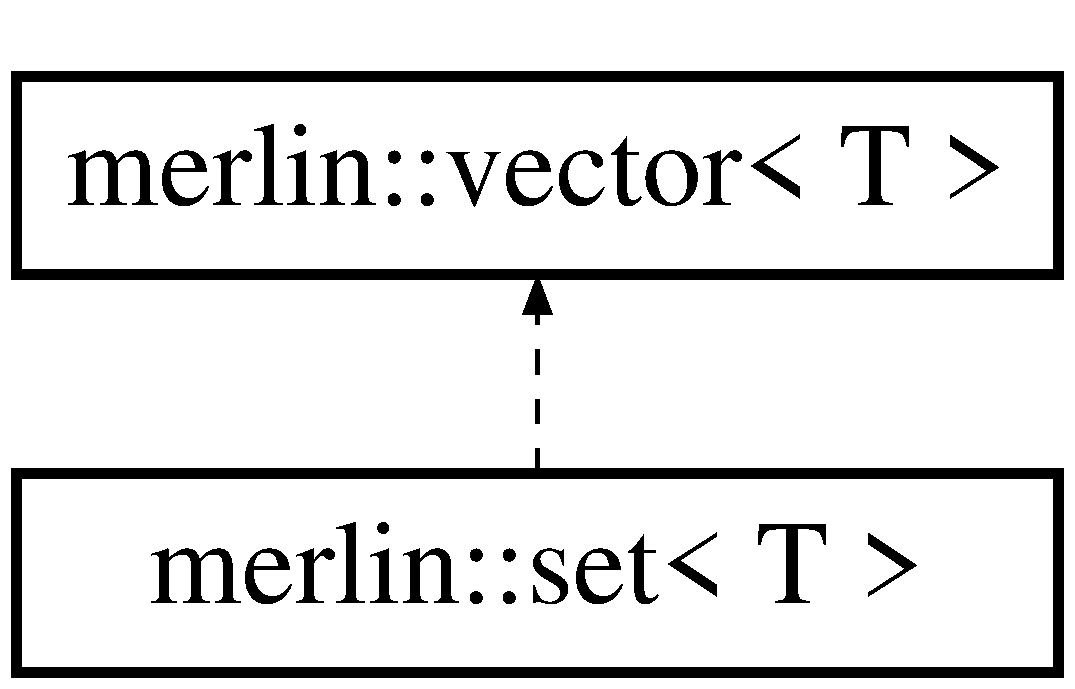
\includegraphics[height=2.000000cm]{classmerlin_1_1set}
\end{center}
\end{figure}
\subsection*{Public Member Functions}
\begin{DoxyCompactItemize}
\item 
size\+\_\+t \hyperlink{classmerlin_1_1set_ac0742e3c7efa8729e1665dc4d0e27784}{size} () const \hypertarget{classmerlin_1_1set_ac0742e3c7efa8729e1665dc4d0e27784}{}\label{classmerlin_1_1set_ac0742e3c7efa8729e1665dc4d0e27784}

\begin{DoxyCompactList}\small\item\em Return container size. \end{DoxyCompactList}\item 
size\+\_\+t \hyperlink{classmerlin_1_1set_ad67b073f6e622b4172d45b94bdf8a84a}{max\+\_\+size} () const \hypertarget{classmerlin_1_1set_ad67b073f6e622b4172d45b94bdf8a84a}{}\label{classmerlin_1_1set_ad67b073f6e622b4172d45b94bdf8a84a}

\begin{DoxyCompactList}\small\item\em Return maximum size of the container. \end{DoxyCompactList}\item 
size\+\_\+t \hyperlink{classmerlin_1_1set_ad3f6a7acc4c9bf242f7f7232e50327bc}{capacity} () const \hypertarget{classmerlin_1_1set_ad3f6a7acc4c9bf242f7f7232e50327bc}{}\label{classmerlin_1_1set_ad3f6a7acc4c9bf242f7f7232e50327bc}

\begin{DoxyCompactList}\small\item\em Return the capacity of the container. \end{DoxyCompactList}\item 
bool \hyperlink{classmerlin_1_1set_a8b606658f0bd7e5b75678110916a3e4a}{empty} () const \hypertarget{classmerlin_1_1set_a8b606658f0bd7e5b75678110916a3e4a}{}\label{classmerlin_1_1set_a8b606658f0bd7e5b75678110916a3e4a}

\begin{DoxyCompactList}\small\item\em Test whether container is empty. \end{DoxyCompactList}\item 
void \hyperlink{classmerlin_1_1set_a320b79b019b9eb53317443c44c92d5a5}{reserve} (size\+\_\+t n)\hypertarget{classmerlin_1_1set_a320b79b019b9eb53317443c44c92d5a5}{}\label{classmerlin_1_1set_a320b79b019b9eb53317443c44c92d5a5}

\begin{DoxyCompactList}\small\item\em Reserve memory for {\itshape n} elements. \end{DoxyCompactList}\item 
void \hyperlink{classmerlin_1_1set_ae57be6d7589cfcc00a8fd582205722f9}{clear} ()\hypertarget{classmerlin_1_1set_ae57be6d7589cfcc00a8fd582205722f9}{}\label{classmerlin_1_1set_ae57be6d7589cfcc00a8fd582205722f9}

\begin{DoxyCompactList}\small\item\em Clear content. \end{DoxyCompactList}\item 
const\+\_\+iterator \hyperlink{classmerlin_1_1set_ac8f64095116304f7edee89c37771e046}{begin} () const \hypertarget{classmerlin_1_1set_ac8f64095116304f7edee89c37771e046}{}\label{classmerlin_1_1set_ac8f64095116304f7edee89c37771e046}

\begin{DoxyCompactList}\small\item\em Return const iterator to beginning. \end{DoxyCompactList}\item 
const\+\_\+iterator \hyperlink{classmerlin_1_1set_a68ae0e206fe3821db7e53d05d347551b}{end} () const \hypertarget{classmerlin_1_1set_a68ae0e206fe3821db7e53d05d347551b}{}\label{classmerlin_1_1set_a68ae0e206fe3821db7e53d05d347551b}

\begin{DoxyCompactList}\small\item\em Return const iterator to end. \end{DoxyCompactList}\item 
const\+\_\+reverse\+\_\+iterator \hyperlink{classmerlin_1_1set_aa0783ca6e1d73d3c51b051a4e3c97434}{rbegin} () const \hypertarget{classmerlin_1_1set_aa0783ca6e1d73d3c51b051a4e3c97434}{}\label{classmerlin_1_1set_aa0783ca6e1d73d3c51b051a4e3c97434}

\begin{DoxyCompactList}\small\item\em Return const reverser iterator to reverse beginning. \end{DoxyCompactList}\item 
const\+\_\+reverse\+\_\+iterator \hyperlink{classmerlin_1_1set_a2b87199b2c744d13285365c94298d238}{rend} () const \hypertarget{classmerlin_1_1set_a2b87199b2c744d13285365c94298d238}{}\label{classmerlin_1_1set_a2b87199b2c744d13285365c94298d238}

\begin{DoxyCompactList}\small\item\em Return const reverse iterator to reverse end. \end{DoxyCompactList}\item 
const T \& \hyperlink{classmerlin_1_1set_a554ef509882e4d14cc0c8dd772eff7a9}{operator\mbox{[}$\,$\mbox{]}} (size\+\_\+t n) const \hypertarget{classmerlin_1_1set_a554ef509882e4d14cc0c8dd772eff7a9}{}\label{classmerlin_1_1set_a554ef509882e4d14cc0c8dd772eff7a9}

\begin{DoxyCompactList}\small\item\em Direct access to n-\/th element. \end{DoxyCompactList}\item 
const T \& \hyperlink{classmerlin_1_1set_af666381d39987a3a00787b0f1e7b9fb3}{at} (size\+\_\+t n) const \hypertarget{classmerlin_1_1set_af666381d39987a3a00787b0f1e7b9fb3}{}\label{classmerlin_1_1set_af666381d39987a3a00787b0f1e7b9fb3}

\begin{DoxyCompactList}\small\item\em Direct access to n-\/th element. \end{DoxyCompactList}\item 
const T \& \hyperlink{classmerlin_1_1set_af82e83415c527fcfeb58be6b52a90e50}{back} () const \hypertarget{classmerlin_1_1set_af82e83415c527fcfeb58be6b52a90e50}{}\label{classmerlin_1_1set_af82e83415c527fcfeb58be6b52a90e50}

\begin{DoxyCompactList}\small\item\em Direct access to the last element. \end{DoxyCompactList}\item 
const T \& \hyperlink{classmerlin_1_1set_af270bbb3466f328017c06624c134c927}{front} () const \hypertarget{classmerlin_1_1set_af270bbb3466f328017c06624c134c927}{}\label{classmerlin_1_1set_af270bbb3466f328017c06624c134c927}

\begin{DoxyCompactList}\small\item\em Direct access to the first element. \end{DoxyCompactList}\item 
const\+\_\+iterator \hyperlink{classmerlin_1_1set_a7006853510da98c34586a5fc07a43187}{find} (const T \&x) const \hypertarget{classmerlin_1_1set_a7006853510da98c34586a5fc07a43187}{}\label{classmerlin_1_1set_a7006853510da98c34586a5fc07a43187}

\begin{DoxyCompactList}\small\item\em Find a given element in the container. \end{DoxyCompactList}\item 
\hyperlink{classmerlin_1_1set_a435150b8aca2440576d6d2d11cb17e22}{set} (size\+\_\+t \hyperlink{classmerlin_1_1set_ad3f6a7acc4c9bf242f7f7232e50327bc}{capacity}=10)\hypertarget{classmerlin_1_1set_a435150b8aca2440576d6d2d11cb17e22}{}\label{classmerlin_1_1set_a435150b8aca2440576d6d2d11cb17e22}

\begin{DoxyCompactList}\small\item\em Default constructor. \end{DoxyCompactList}\item 
\hyperlink{classmerlin_1_1set_afcc09e984c6dad4310b4dd1e53df02f0}{set} (const \hyperlink{classmerlin_1_1set}{set} \&v)\hypertarget{classmerlin_1_1set_afcc09e984c6dad4310b4dd1e53df02f0}{}\label{classmerlin_1_1set_afcc09e984c6dad4310b4dd1e53df02f0}

\begin{DoxyCompactList}\small\item\em Copy-\/constructor. \end{DoxyCompactList}\item 
{\footnotesize template$<$class in\+Iter $>$ }\\\hyperlink{classmerlin_1_1set_aa945e76777e7d527be7487072029f359}{set} (in\+Iter first, in\+Iter last)\hypertarget{classmerlin_1_1set_aa945e76777e7d527be7487072029f359}{}\label{classmerlin_1_1set_aa945e76777e7d527be7487072029f359}

\begin{DoxyCompactList}\small\item\em Constructor with input iterators. \end{DoxyCompactList}\item 
\hyperlink{classmerlin_1_1set}{set}$<$ T $>$ \& \hyperlink{classmerlin_1_1set_ab44b00506d4ba9a6209bba0dc2df7df7}{operator=} (const \hyperlink{classmerlin_1_1set}{set}$<$ T $>$ \&s)\hypertarget{classmerlin_1_1set_ab44b00506d4ba9a6209bba0dc2df7df7}{}\label{classmerlin_1_1set_ab44b00506d4ba9a6209bba0dc2df7df7}

\begin{DoxyCompactList}\small\item\em Assignment operator. \end{DoxyCompactList}\item 
\hyperlink{classmerlin_1_1set_a96d2340e84d377b1a9a8b62123e9a7c1}{$\sim$set} ()\hypertarget{classmerlin_1_1set_a96d2340e84d377b1a9a8b62123e9a7c1}{}\label{classmerlin_1_1set_a96d2340e84d377b1a9a8b62123e9a7c1}

\begin{DoxyCompactList}\small\item\em Set destructor. \end{DoxyCompactList}\item 
\hyperlink{classmerlin_1_1set}{set}$<$ T $>$ \hyperlink{classmerlin_1_1set_a13ebc00884144896d3cafb6552cd760a}{operator$\vert$} (const \hyperlink{classmerlin_1_1set}{set}$<$ T $>$ \&) const \hypertarget{classmerlin_1_1set_a13ebc00884144896d3cafb6552cd760a}{}\label{classmerlin_1_1set_a13ebc00884144896d3cafb6552cd760a}

\begin{DoxyCompactList}\small\item\em Union. \end{DoxyCompactList}\item 
\hyperlink{classmerlin_1_1set}{set}$<$ T $>$ \hyperlink{classmerlin_1_1set_affa59b7a3c25985c36cfa8d13f005f5c}{operator+} (const \hyperlink{classmerlin_1_1set}{set}$<$ T $>$ \&) const \hypertarget{classmerlin_1_1set_affa59b7a3c25985c36cfa8d13f005f5c}{}\label{classmerlin_1_1set_affa59b7a3c25985c36cfa8d13f005f5c}

\begin{DoxyCompactList}\small\item\em Union. \end{DoxyCompactList}\item 
\hyperlink{classmerlin_1_1set}{set}$<$ T $>$ \hyperlink{classmerlin_1_1set_a53f01cf729d6762f3aad050a3c80ad74}{operator/} (const \hyperlink{classmerlin_1_1set}{set}$<$ T $>$ \&) const \hypertarget{classmerlin_1_1set_a53f01cf729d6762f3aad050a3c80ad74}{}\label{classmerlin_1_1set_a53f01cf729d6762f3aad050a3c80ad74}

\begin{DoxyCompactList}\small\item\em Set-\/diff. \end{DoxyCompactList}\item 
\hyperlink{classmerlin_1_1set}{set}$<$ T $>$ \hyperlink{classmerlin_1_1set_ab5230f892f1e830152477325ad03985f}{operator-\/} (const \hyperlink{classmerlin_1_1set}{set}$<$ T $>$ \&) const \hypertarget{classmerlin_1_1set_ab5230f892f1e830152477325ad03985f}{}\label{classmerlin_1_1set_ab5230f892f1e830152477325ad03985f}

\begin{DoxyCompactList}\small\item\em Set-\/diff. \end{DoxyCompactList}\item 
\hyperlink{classmerlin_1_1set}{set}$<$ T $>$ \hyperlink{classmerlin_1_1set_ab140657855d16aafab6f16cb57409a64}{operator\&} (const \hyperlink{classmerlin_1_1set}{set}$<$ T $>$ \&) const \hypertarget{classmerlin_1_1set_ab140657855d16aafab6f16cb57409a64}{}\label{classmerlin_1_1set_ab140657855d16aafab6f16cb57409a64}

\begin{DoxyCompactList}\small\item\em Intersect. \end{DoxyCompactList}\item 
\hyperlink{classmerlin_1_1set}{set}$<$ T $>$ \hyperlink{classmerlin_1_1set_a054f035d0051b753bc55b72067200dc5}{operator$^\wedge$} (const \hyperlink{classmerlin_1_1set}{set}$<$ T $>$ \&) const \hypertarget{classmerlin_1_1set_a054f035d0051b753bc55b72067200dc5}{}\label{classmerlin_1_1set_a054f035d0051b753bc55b72067200dc5}

\begin{DoxyCompactList}\small\item\em Symm set diff. \end{DoxyCompactList}\item 
\hyperlink{classmerlin_1_1set}{set}$<$ T $>$ \hyperlink{classmerlin_1_1set_a3c2bd97561ea5e7cd651cb4d6bcbf677}{operator$\vert$} (const T \&) const \hypertarget{classmerlin_1_1set_a3c2bd97561ea5e7cd651cb4d6bcbf677}{}\label{classmerlin_1_1set_a3c2bd97561ea5e7cd651cb4d6bcbf677}

\begin{DoxyCompactList}\small\item\em Union. \end{DoxyCompactList}\item 
\hyperlink{classmerlin_1_1set}{set}$<$ T $>$ \hyperlink{classmerlin_1_1set_a3da3e8798b664f7e746a6729e96a3536}{operator+} (const T \&) const \hypertarget{classmerlin_1_1set_a3da3e8798b664f7e746a6729e96a3536}{}\label{classmerlin_1_1set_a3da3e8798b664f7e746a6729e96a3536}

\begin{DoxyCompactList}\small\item\em Union. \end{DoxyCompactList}\item 
\hyperlink{classmerlin_1_1set}{set}$<$ T $>$ \hyperlink{classmerlin_1_1set_a24b9eb766ec4c25ded1309bcd1c39526}{operator/} (const T \&) const \hypertarget{classmerlin_1_1set_a24b9eb766ec4c25ded1309bcd1c39526}{}\label{classmerlin_1_1set_a24b9eb766ec4c25ded1309bcd1c39526}

\begin{DoxyCompactList}\small\item\em Set-\/diff. \end{DoxyCompactList}\item 
\hyperlink{classmerlin_1_1set}{set}$<$ T $>$ \hyperlink{classmerlin_1_1set_af97e3a5d5f7c4e8b3e9a19faef1f4ee2}{operator-\/} (const T \&) const \hypertarget{classmerlin_1_1set_af97e3a5d5f7c4e8b3e9a19faef1f4ee2}{}\label{classmerlin_1_1set_af97e3a5d5f7c4e8b3e9a19faef1f4ee2}

\begin{DoxyCompactList}\small\item\em Set-\/diff. \end{DoxyCompactList}\item 
\hyperlink{classmerlin_1_1set}{set}$<$ T $>$ \hyperlink{classmerlin_1_1set_a5f97ef2bb5f230848ad018d86eb5a4b2}{operator\&} (const T \&) const \hypertarget{classmerlin_1_1set_a5f97ef2bb5f230848ad018d86eb5a4b2}{}\label{classmerlin_1_1set_a5f97ef2bb5f230848ad018d86eb5a4b2}

\begin{DoxyCompactList}\small\item\em Intersect. \end{DoxyCompactList}\item 
\hyperlink{classmerlin_1_1set}{set}$<$ T $>$ \hyperlink{classmerlin_1_1set_ac83716f6188e49336951c005ce2dc37d}{operator$^\wedge$} (const T \&) const \hypertarget{classmerlin_1_1set_ac83716f6188e49336951c005ce2dc37d}{}\label{classmerlin_1_1set_ac83716f6188e49336951c005ce2dc37d}

\begin{DoxyCompactList}\small\item\em Symm set diff. \end{DoxyCompactList}\item 
\hyperlink{classmerlin_1_1set}{set}$<$ T $>$ \& \hyperlink{classmerlin_1_1set_a61a296737e57dae6df4cfc2a76248e03}{operator$\vert$=} (const \hyperlink{classmerlin_1_1set}{set}$<$ T $>$ \&)\hypertarget{classmerlin_1_1set_a61a296737e57dae6df4cfc2a76248e03}{}\label{classmerlin_1_1set_a61a296737e57dae6df4cfc2a76248e03}

\begin{DoxyCompactList}\small\item\em Union. \end{DoxyCompactList}\item 
\hyperlink{classmerlin_1_1set}{set}$<$ T $>$ \& \hyperlink{classmerlin_1_1set_af383998860d966997045b18e9d801439}{operator+=} (const \hyperlink{classmerlin_1_1set}{set}$<$ T $>$ \&)\hypertarget{classmerlin_1_1set_af383998860d966997045b18e9d801439}{}\label{classmerlin_1_1set_af383998860d966997045b18e9d801439}

\begin{DoxyCompactList}\small\item\em Union. \end{DoxyCompactList}\item 
\hyperlink{classmerlin_1_1set}{set}$<$ T $>$ \& \hyperlink{classmerlin_1_1set_a5bb76573ee049dd6003155c87f468a80}{operator/=} (const \hyperlink{classmerlin_1_1set}{set}$<$ T $>$ \&)\hypertarget{classmerlin_1_1set_a5bb76573ee049dd6003155c87f468a80}{}\label{classmerlin_1_1set_a5bb76573ee049dd6003155c87f468a80}

\begin{DoxyCompactList}\small\item\em Set-\/diff. \end{DoxyCompactList}\item 
\hyperlink{classmerlin_1_1set}{set}$<$ T $>$ \& \hyperlink{classmerlin_1_1set_a8e5f0d149fec50878e7cc767e683f304}{operator-\/=} (const \hyperlink{classmerlin_1_1set}{set}$<$ T $>$ \&)\hypertarget{classmerlin_1_1set_a8e5f0d149fec50878e7cc767e683f304}{}\label{classmerlin_1_1set_a8e5f0d149fec50878e7cc767e683f304}

\begin{DoxyCompactList}\small\item\em Set-\/diff. \end{DoxyCompactList}\item 
\hyperlink{classmerlin_1_1set}{set}$<$ T $>$ \& \hyperlink{classmerlin_1_1set_a4428ef791cee89dd567785aba416e2e8}{operator\&=} (const \hyperlink{classmerlin_1_1set}{set}$<$ T $>$ \&)\hypertarget{classmerlin_1_1set_a4428ef791cee89dd567785aba416e2e8}{}\label{classmerlin_1_1set_a4428ef791cee89dd567785aba416e2e8}

\begin{DoxyCompactList}\small\item\em Intersect. \end{DoxyCompactList}\item 
\hyperlink{classmerlin_1_1set}{set}$<$ T $>$ \& \hyperlink{classmerlin_1_1set_a18a65ff994f1a9c6bbf2fbca253a2ebf}{operator$^\wedge$=} (const \hyperlink{classmerlin_1_1set}{set}$<$ T $>$ \&)\hypertarget{classmerlin_1_1set_a18a65ff994f1a9c6bbf2fbca253a2ebf}{}\label{classmerlin_1_1set_a18a65ff994f1a9c6bbf2fbca253a2ebf}

\begin{DoxyCompactList}\small\item\em Symm set diff. \end{DoxyCompactList}\item 
\hyperlink{classmerlin_1_1set}{set}$<$ T $>$ \& \hyperlink{classmerlin_1_1set_a40a231741cd7852f3cdf4f8a0e49f691}{operator$\vert$=} (const T \&)\hypertarget{classmerlin_1_1set_a40a231741cd7852f3cdf4f8a0e49f691}{}\label{classmerlin_1_1set_a40a231741cd7852f3cdf4f8a0e49f691}

\begin{DoxyCompactList}\small\item\em Union. \end{DoxyCompactList}\item 
\hyperlink{classmerlin_1_1set}{set}$<$ T $>$ \& \hyperlink{classmerlin_1_1set_a97a67ab3addec83ef5ddff361ba29b7e}{operator+=} (const T \&)\hypertarget{classmerlin_1_1set_a97a67ab3addec83ef5ddff361ba29b7e}{}\label{classmerlin_1_1set_a97a67ab3addec83ef5ddff361ba29b7e}

\begin{DoxyCompactList}\small\item\em Union. \end{DoxyCompactList}\item 
\hyperlink{classmerlin_1_1set}{set}$<$ T $>$ \& \hyperlink{classmerlin_1_1set_a5fb011df323a4809972209667e002935}{operator/=} (const T \&)\hypertarget{classmerlin_1_1set_a5fb011df323a4809972209667e002935}{}\label{classmerlin_1_1set_a5fb011df323a4809972209667e002935}

\begin{DoxyCompactList}\small\item\em Set-\/diff. \end{DoxyCompactList}\item 
\hyperlink{classmerlin_1_1set}{set}$<$ T $>$ \& \hyperlink{classmerlin_1_1set_a90e101a698c09d1fdb4a2b0c540e91ff}{operator-\/=} (const T \&)\hypertarget{classmerlin_1_1set_a90e101a698c09d1fdb4a2b0c540e91ff}{}\label{classmerlin_1_1set_a90e101a698c09d1fdb4a2b0c540e91ff}

\begin{DoxyCompactList}\small\item\em Set-\/diff. \end{DoxyCompactList}\item 
\hyperlink{classmerlin_1_1set}{set}$<$ T $>$ \& \hyperlink{classmerlin_1_1set_a48df656e6907e78977d765ee59eadb2e}{operator\&=} (const T \&)\hypertarget{classmerlin_1_1set_a48df656e6907e78977d765ee59eadb2e}{}\label{classmerlin_1_1set_a48df656e6907e78977d765ee59eadb2e}

\begin{DoxyCompactList}\small\item\em Intersect. \end{DoxyCompactList}\item 
\hyperlink{classmerlin_1_1set}{set}$<$ T $>$ \& \hyperlink{classmerlin_1_1set_a58d08d3746bbc7d9bf1ec9fbe6451641}{operator$^\wedge$=} (const T \&)\hypertarget{classmerlin_1_1set_a58d08d3746bbc7d9bf1ec9fbe6451641}{}\label{classmerlin_1_1set_a58d08d3746bbc7d9bf1ec9fbe6451641}

\begin{DoxyCompactList}\small\item\em Symm set diff. \end{DoxyCompactList}\item 
void \hyperlink{classmerlin_1_1set_adf61e75f4ccc0c093fa3759619d3f4ff}{remove} (const T \&t)\hypertarget{classmerlin_1_1set_adf61e75f4ccc0c093fa3759619d3f4ff}{}\label{classmerlin_1_1set_adf61e75f4ccc0c093fa3759619d3f4ff}

\begin{DoxyCompactList}\small\item\em Remove a single element. \end{DoxyCompactList}\item 
void \hyperlink{classmerlin_1_1set_a12ca303df4af43659a892188eeda5272}{add} (const T \&t)\hypertarget{classmerlin_1_1set_a12ca303df4af43659a892188eeda5272}{}\label{classmerlin_1_1set_a12ca303df4af43659a892188eeda5272}

\begin{DoxyCompactList}\small\item\em Add a single element. \end{DoxyCompactList}\item 
void \hyperlink{classmerlin_1_1set_a52af645785b5b689c95ddb4d0e2774dc}{swap} (\hyperlink{classmerlin_1_1set}{set}$<$ T $>$ \&v)\hypertarget{classmerlin_1_1set_a52af645785b5b689c95ddb4d0e2774dc}{}\label{classmerlin_1_1set_a52af645785b5b689c95ddb4d0e2774dc}

\begin{DoxyCompactList}\small\item\em Swap content. \end{DoxyCompactList}\item 
bool \hyperlink{classmerlin_1_1set_a4721e77f71f2771f4c5b3873f4f3259f}{operator==} (const \hyperlink{classmerlin_1_1set}{set}$<$ T $>$ \&t) const \hypertarget{classmerlin_1_1set_a4721e77f71f2771f4c5b3873f4f3259f}{}\label{classmerlin_1_1set_a4721e77f71f2771f4c5b3873f4f3259f}

\begin{DoxyCompactList}\small\item\em Equality operator over lexicographic order. \end{DoxyCompactList}\item 
bool \hyperlink{classmerlin_1_1set_aafa2d337583501c51a520d46f64a3ef3}{operator!=} (const \hyperlink{classmerlin_1_1set}{set}$<$ T $>$ \&t) const \hypertarget{classmerlin_1_1set_aafa2d337583501c51a520d46f64a3ef3}{}\label{classmerlin_1_1set_aafa2d337583501c51a520d46f64a3ef3}

\begin{DoxyCompactList}\small\item\em Not-\/equal operator over lexicographic order. \end{DoxyCompactList}\item 
bool \hyperlink{classmerlin_1_1set_ae1e9ec4a3a6cc07b5a04b1e6605b7b22}{operator$<$} (const \hyperlink{classmerlin_1_1set}{set}$<$ T $>$ \&t) const \hypertarget{classmerlin_1_1set_ae1e9ec4a3a6cc07b5a04b1e6605b7b22}{}\label{classmerlin_1_1set_ae1e9ec4a3a6cc07b5a04b1e6605b7b22}

\begin{DoxyCompactList}\small\item\em Less-\/than operator over lexicographic order. \end{DoxyCompactList}\item 
bool \hyperlink{classmerlin_1_1set_acd79b5291a0c3eff64f993cf25031418}{operator$<$=} (const \hyperlink{classmerlin_1_1set}{set}$<$ T $>$ \&t) const \hypertarget{classmerlin_1_1set_acd79b5291a0c3eff64f993cf25031418}{}\label{classmerlin_1_1set_acd79b5291a0c3eff64f993cf25031418}

\begin{DoxyCompactList}\small\item\em Less-\/or-\/equal-\/than operator over lexicographic order. \end{DoxyCompactList}\item 
bool \hyperlink{classmerlin_1_1set_a8fc807637ddc148480a9d155b2f6998f}{operator$>$} (const \hyperlink{classmerlin_1_1set}{set}$<$ T $>$ \&t) const \hypertarget{classmerlin_1_1set_a8fc807637ddc148480a9d155b2f6998f}{}\label{classmerlin_1_1set_a8fc807637ddc148480a9d155b2f6998f}

\begin{DoxyCompactList}\small\item\em Greater-\/than operator over lexicographic order. \end{DoxyCompactList}\item 
bool \hyperlink{classmerlin_1_1set_a27f64ae1e7ad2e08df34a5dbed0a4d26}{operator$>$=} (const \hyperlink{classmerlin_1_1set}{set}$<$ T $>$ \&t) const \hypertarget{classmerlin_1_1set_a27f64ae1e7ad2e08df34a5dbed0a4d26}{}\label{classmerlin_1_1set_a27f64ae1e7ad2e08df34a5dbed0a4d26}

\begin{DoxyCompactList}\small\item\em Greater-\/or-\/equal-\/than operator over lexicographic order. \end{DoxyCompactList}\end{DoxyCompactItemize}
\subsection*{Protected Member Functions}
\begin{DoxyCompactItemize}
\item 
void \hyperlink{classmerlin_1_1set_a772e18b99eaea86f8a78f07cf6263238}{update} (void)\hypertarget{classmerlin_1_1set_a772e18b99eaea86f8a78f07cf6263238}{}\label{classmerlin_1_1set_a772e18b99eaea86f8a78f07cf6263238}

\begin{DoxyCompactList}\small\item\em Update container. \end{DoxyCompactList}\item 
void \hyperlink{classmerlin_1_1set_a9492b2fb9afeea31d559664bb9afcbb3}{resize} (size\+\_\+t n, const T \&t=T())\hypertarget{classmerlin_1_1set_a9492b2fb9afeea31d559664bb9afcbb3}{}\label{classmerlin_1_1set_a9492b2fb9afeea31d559664bb9afcbb3}

\begin{DoxyCompactList}\small\item\em Resize container. \end{DoxyCompactList}\item 
iterator \hyperlink{classmerlin_1_1set_adc4f7aeff8a337c7b3897b54616849cc}{\+\_\+begin} ()\hypertarget{classmerlin_1_1set_adc4f7aeff8a337c7b3897b54616849cc}{}\label{classmerlin_1_1set_adc4f7aeff8a337c7b3897b54616849cc}

\begin{DoxyCompactList}\small\item\em Return iterator to beginning. \end{DoxyCompactList}\item 
iterator \hyperlink{classmerlin_1_1set_ad87a431a0006ff8608b17515648c8d95}{\+\_\+end} ()\hypertarget{classmerlin_1_1set_ad87a431a0006ff8608b17515648c8d95}{}\label{classmerlin_1_1set_ad87a431a0006ff8608b17515648c8d95}

\begin{DoxyCompactList}\small\item\em Return iterator to end. \end{DoxyCompactList}\item 
reverse\+\_\+iterator \hyperlink{classmerlin_1_1set_ae77c35b12604b58b663e10f3b94799f0}{\+\_\+rbegin} ()\hypertarget{classmerlin_1_1set_ae77c35b12604b58b663e10f3b94799f0}{}\label{classmerlin_1_1set_ae77c35b12604b58b663e10f3b94799f0}

\begin{DoxyCompactList}\small\item\em Return reverse iterator to reverse beginning. \end{DoxyCompactList}\item 
reverse\+\_\+iterator \hyperlink{classmerlin_1_1set_a5ab9d534c39d7ae4875598e2ee4b9174}{\+\_\+rend} ()\hypertarget{classmerlin_1_1set_a5ab9d534c39d7ae4875598e2ee4b9174}{}\label{classmerlin_1_1set_a5ab9d534c39d7ae4875598e2ee4b9174}

\begin{DoxyCompactList}\small\item\em Return reverse iterator to reverse end. \end{DoxyCompactList}\end{DoxyCompactItemize}
\subsection*{Additional Inherited Members}


\subsection{Detailed Description}
\subsubsection*{template$<$class T$>$\\*
class merlin\+::set$<$ T $>$}

Set container storing unique elements following a specific order. 

Definition at line 45 of file set.\+h.



The documentation for this class was generated from the following file\+:\begin{DoxyCompactItemize}
\item 
src/include/\hyperlink{set_8h}{set.\+h}\end{DoxyCompactItemize}

\hypertarget{structmerlin_1_1ijgp_1_1sPair}{}\section{merlin\+:\+:ijgp\+:\+:s\+Pair Struct Reference}
\label{structmerlin_1_1ijgp_1_1sPair}\index{merlin\+::ijgp\+::s\+Pair@{merlin\+::ijgp\+::s\+Pair}}


Helper class for pairs of sorted indices.  




{\ttfamily \#include $<$ijgp.\+h$>$}



Inherits pair$<$ size\+\_\+t, size\+\_\+t $>$.



\subsection{Detailed Description}
Helper class for pairs of sorted indices. 

Definition at line 484 of file ijgp.\+h.



The documentation for this struct was generated from the following file\+:\begin{DoxyCompactItemize}
\item 
src/include/\hyperlink{ijgp_8h}{ijgp.\+h}\end{DoxyCompactItemize}

\hypertarget{structmerlin_1_1jglp_1_1sPair}{}\section{merlin\+:\+:jglp\+:\+:s\+Pair Struct Reference}
\label{structmerlin_1_1jglp_1_1sPair}\index{merlin\+::jglp\+::s\+Pair@{merlin\+::jglp\+::s\+Pair}}


Helper class for pairs of sorted indices.  




{\ttfamily \#include $<$jglp.\+h$>$}



Inherits pair$<$ size\+\_\+t, size\+\_\+t $>$.



\subsection{Detailed Description}
Helper class for pairs of sorted indices. 

Definition at line 305 of file jglp.\+h.



The documentation for this struct was generated from the following file\+:\begin{DoxyCompactItemize}
\item 
src/include/\hyperlink{jglp_8h}{jglp.\+h}\end{DoxyCompactItemize}

\hypertarget{classmerlin_1_1subindex}{}\section{merlin\+:\+:subindex Class Reference}
\label{classmerlin_1_1subindex}\index{merlin\+::subindex@{merlin\+::subindex}}


Subindex for iterating over configurations of a set of variables.  




{\ttfamily \#include $<$index.\+h$>$}

\subsection*{Public Types}
\begin{DoxyCompactItemize}
\item 
typedef \hyperlink{classmerlin_1_1variable__set_a05d7a8291564fa7fb236a5e9cb65c734}{variable\+\_\+set\+::vsize} \hyperlink{classmerlin_1_1subindex_a85a7fddb94bd83a77a4a73293c5d613a}{vsize}\hypertarget{classmerlin_1_1subindex_a85a7fddb94bd83a77a4a73293c5d613a}{}\label{classmerlin_1_1subindex_a85a7fddb94bd83a77a4a73293c5d613a}

\begin{DoxyCompactList}\small\item\em Variable index. \end{DoxyCompactList}\end{DoxyCompactItemize}
\subsection*{Public Member Functions}
\begin{DoxyCompactItemize}
\item 
\hyperlink{classmerlin_1_1subindex_a4dc11ac00d5b35a1a576c079b61ba482}{subindex} (const \hyperlink{classmerlin_1_1variable__set}{variable\+\_\+set} \&full, const \hyperlink{classmerlin_1_1variable__set}{variable\+\_\+set} \&sub)\hypertarget{classmerlin_1_1subindex_a4dc11ac00d5b35a1a576c079b61ba482}{}\label{classmerlin_1_1subindex_a4dc11ac00d5b35a1a576c079b61ba482}

\begin{DoxyCompactList}\small\item\em Construct the sub-\/index. \end{DoxyCompactList}\item 
\hyperlink{classmerlin_1_1subindex_a3e0464e36f33fb7ceb0a797ff5296d32}{subindex} (const \hyperlink{classmerlin_1_1subindex}{subindex} \&s)\hypertarget{classmerlin_1_1subindex_a3e0464e36f33fb7ceb0a797ff5296d32}{}\label{classmerlin_1_1subindex_a3e0464e36f33fb7ceb0a797ff5296d32}

\begin{DoxyCompactList}\small\item\em Copy (constructor) the sub-\/index. \end{DoxyCompactList}\item 
\hyperlink{classmerlin_1_1subindex_a2d5988647a46e6373084f968f1a623bc}{$\sim$subindex} (void)\hypertarget{classmerlin_1_1subindex_a2d5988647a46e6373084f968f1a623bc}{}\label{classmerlin_1_1subindex_a2d5988647a46e6373084f968f1a623bc}

\begin{DoxyCompactList}\small\item\em Sub-\/index destructor. \end{DoxyCompactList}\item 
\hyperlink{classmerlin_1_1subindex}{subindex} \& \hyperlink{classmerlin_1_1subindex_a0acd5e4bf8b9ed42b76c1c67ea9ad13e}{reset} ()\hypertarget{classmerlin_1_1subindex_a0acd5e4bf8b9ed42b76c1c67ea9ad13e}{}\label{classmerlin_1_1subindex_a0acd5e4bf8b9ed42b76c1c67ea9ad13e}

\begin{DoxyCompactList}\small\item\em Reset the sub-\/index. \end{DoxyCompactList}\item 
size\+\_\+t \hyperlink{classmerlin_1_1subindex_a013078eb23f9c472347866c67951ce15}{end} ()\hypertarget{classmerlin_1_1subindex_a013078eb23f9c472347866c67951ce15}{}\label{classmerlin_1_1subindex_a013078eb23f9c472347866c67951ce15}

\begin{DoxyCompactList}\small\item\em Return the last position in the sub-\/index. \end{DoxyCompactList}\item 
\hyperlink{classmerlin_1_1subindex}{subindex} \& \hyperlink{classmerlin_1_1subindex_a76103ec045336205b10c9db20598c44c}{operator++} (void)\hypertarget{classmerlin_1_1subindex_a76103ec045336205b10c9db20598c44c}{}\label{classmerlin_1_1subindex_a76103ec045336205b10c9db20598c44c}

\begin{DoxyCompactList}\small\item\em Prefix addition operator. \end{DoxyCompactList}\item 
\hyperlink{classmerlin_1_1subindex}{subindex} \hyperlink{classmerlin_1_1subindex_ae75380581f8cbdb251138b0bc6ad1ce9}{operator++} (int)\hypertarget{classmerlin_1_1subindex_ae75380581f8cbdb251138b0bc6ad1ce9}{}\label{classmerlin_1_1subindex_ae75380581f8cbdb251138b0bc6ad1ce9}

\begin{DoxyCompactList}\small\item\em Postfix addition using prefix and copy. \end{DoxyCompactList}\item 
\hyperlink{classmerlin_1_1subindex_afe9fff1d825256a4e94b982716db9da7}{operator size\+\_\+t} () const \hypertarget{classmerlin_1_1subindex_afe9fff1d825256a4e94b982716db9da7}{}\label{classmerlin_1_1subindex_afe9fff1d825256a4e94b982716db9da7}

\begin{DoxyCompactList}\small\item\em Conversion to index value. \end{DoxyCompactList}\end{DoxyCompactItemize}
\subsection*{Public Attributes}
\begin{DoxyCompactItemize}
\item 
\hyperlink{classmerlin_1_1subindex_a85a7fddb94bd83a77a4a73293c5d613a}{vsize} \hyperlink{classmerlin_1_1subindex_ace8d4c5272d59793482b2cfaae5c84b4}{m\+\_\+idx}\hypertarget{classmerlin_1_1subindex_ace8d4c5272d59793482b2cfaae5c84b4}{}\label{classmerlin_1_1subindex_ace8d4c5272d59793482b2cfaae5c84b4}

\begin{DoxyCompactList}\small\item\em Current index position. \end{DoxyCompactList}\item 
\hyperlink{classmerlin_1_1subindex_a85a7fddb94bd83a77a4a73293c5d613a}{vsize} \hyperlink{classmerlin_1_1subindex_ae39e046222b12314a76e22b38a390eaa}{m\+\_\+end}\hypertarget{classmerlin_1_1subindex_ae39e046222b12314a76e22b38a390eaa}{}\label{classmerlin_1_1subindex_ae39e046222b12314a76e22b38a390eaa}

\begin{DoxyCompactList}\small\item\em Last position. \end{DoxyCompactList}\item 
\hyperlink{classmerlin_1_1subindex_a85a7fddb94bd83a77a4a73293c5d613a}{vsize} \hyperlink{classmerlin_1_1subindex_a2acf7a181ba7c7e4550303b45f655af3}{m\+\_\+nd}\hypertarget{classmerlin_1_1subindex_a2acf7a181ba7c7e4550303b45f655af3}{}\label{classmerlin_1_1subindex_a2acf7a181ba7c7e4550303b45f655af3}

\begin{DoxyCompactList}\small\item\em Number of variables in the sub-\/index. \end{DoxyCompactList}\item 
\hyperlink{classmerlin_1_1subindex_a85a7fddb94bd83a77a4a73293c5d613a}{vsize} $\ast$ \hyperlink{classmerlin_1_1subindex_acd8990d2aa72a0650ecb66a15274cc8f}{m\+\_\+state}\hypertarget{classmerlin_1_1subindex_acd8990d2aa72a0650ecb66a15274cc8f}{}\label{classmerlin_1_1subindex_acd8990d2aa72a0650ecb66a15274cc8f}

\begin{DoxyCompactList}\small\item\em Vector of variable-\/indices (values) for the current position (1-\/based) \end{DoxyCompactList}\item 
const \hyperlink{classmerlin_1_1subindex_a85a7fddb94bd83a77a4a73293c5d613a}{vsize} $\ast$ \hyperlink{classmerlin_1_1subindex_ab61eacce232dc804e1c12bf9b0445c3a}{m\+\_\+dims}\hypertarget{classmerlin_1_1subindex_ab61eacce232dc804e1c12bf9b0445c3a}{}\label{classmerlin_1_1subindex_ab61eacce232dc804e1c12bf9b0445c3a}

\begin{DoxyCompactList}\small\item\em Dimensions of each variable. \end{DoxyCompactList}\item 
bool $\ast$ \hyperlink{classmerlin_1_1subindex_a5b9ae8404bdc32036922ee2c220da5dc}{m\+\_\+skipped}\hypertarget{classmerlin_1_1subindex_a5b9ae8404bdc32036922ee2c220da5dc}{}\label{classmerlin_1_1subindex_a5b9ae8404bdc32036922ee2c220da5dc}

\begin{DoxyCompactList}\small\item\em Variables not included in the sub-\/index. \end{DoxyCompactList}\item 
\hyperlink{classmerlin_1_1subindex_a85a7fddb94bd83a77a4a73293c5d613a}{vsize} $\ast$ \hyperlink{classmerlin_1_1subindex_a1dde0ca8f1664ef945f74070711f6816}{m\+\_\+add}\hypertarget{classmerlin_1_1subindex_a1dde0ca8f1664ef945f74070711f6816}{}\label{classmerlin_1_1subindex_a1dde0ca8f1664ef945f74070711f6816}

\begin{DoxyCompactList}\small\item\em How much to add when we increment. \end{DoxyCompactList}\item 
\hyperlink{classmerlin_1_1subindex_a85a7fddb94bd83a77a4a73293c5d613a}{vsize} $\ast$ \hyperlink{classmerlin_1_1subindex_a4366c38983a38191319f53bbee8461ad}{m\+\_\+subtract}\hypertarget{classmerlin_1_1subindex_a4366c38983a38191319f53bbee8461ad}{}\label{classmerlin_1_1subindex_a4366c38983a38191319f53bbee8461ad}

\begin{DoxyCompactList}\small\item\em How much to subtract when we wrap each variable. \end{DoxyCompactList}\end{DoxyCompactItemize}
\subsection*{Friends}
\begin{DoxyCompactItemize}
\item 
std\+::ostream \& \hyperlink{classmerlin_1_1subindex_ae3af7027432ef1db960d32c52007877d}{operator$<$$<$} (std\+::ostream \&os, const \hyperlink{classmerlin_1_1subindex}{subindex} \&s)\hypertarget{classmerlin_1_1subindex_ae3af7027432ef1db960d32c52007877d}{}\label{classmerlin_1_1subindex_ae3af7027432ef1db960d32c52007877d}

\begin{DoxyCompactList}\small\item\em Output operator. \end{DoxyCompactList}\end{DoxyCompactItemize}


\subsection{Detailed Description}
Subindex for iterating over configurations of a set of variables. 

Definition at line 36 of file index.\+h.



The documentation for this class was generated from the following file\+:\begin{DoxyCompactItemize}
\item 
src/include/\hyperlink{index_8h}{index.\+h}\end{DoxyCompactItemize}

\hypertarget{classmerlin_1_1superindex}{}\section{merlin\+:\+:superindex Class Reference}
\label{classmerlin_1_1superindex}\index{merlin\+::superindex@{merlin\+::superindex}}


Superindex for iterating over the configurations of a set of variables.  




{\ttfamily \#include $<$index.\+h$>$}

\subsection*{Public Types}
\begin{DoxyCompactItemize}
\item 
typedef \hyperlink{classmerlin_1_1variable__set_a05d7a8291564fa7fb236a5e9cb65c734}{variable\+\_\+set\+::vsize} \hyperlink{classmerlin_1_1superindex_a4e63d0617c6b351c664cdfd406686d62}{vsize}\hypertarget{classmerlin_1_1superindex_a4e63d0617c6b351c664cdfd406686d62}{}\label{classmerlin_1_1superindex_a4e63d0617c6b351c664cdfd406686d62}

\begin{DoxyCompactList}\small\item\em Variable index. \end{DoxyCompactList}\end{DoxyCompactItemize}
\subsection*{Public Member Functions}
\begin{DoxyCompactItemize}
\item 
\hyperlink{classmerlin_1_1superindex_a9fdcd5396269adc20332a46f8e0e33e8}{superindex} (const \hyperlink{classmerlin_1_1variable__set}{variable\+\_\+set} \&full, const \hyperlink{classmerlin_1_1variable__set}{variable\+\_\+set} \&sub, size\+\_\+t offset)\hypertarget{classmerlin_1_1superindex_a9fdcd5396269adc20332a46f8e0e33e8}{}\label{classmerlin_1_1superindex_a9fdcd5396269adc20332a46f8e0e33e8}

\begin{DoxyCompactList}\small\item\em Construct the super index. \end{DoxyCompactList}\item 
\hyperlink{classmerlin_1_1superindex_a6ca2a8c735a9542940509299e5d0f4b2}{superindex} (const \hyperlink{classmerlin_1_1superindex}{superindex} \&s)\hypertarget{classmerlin_1_1superindex_a6ca2a8c735a9542940509299e5d0f4b2}{}\label{classmerlin_1_1superindex_a6ca2a8c735a9542940509299e5d0f4b2}

\begin{DoxyCompactList}\small\item\em Copy (constructor) a super index. \end{DoxyCompactList}\item 
\hyperlink{classmerlin_1_1superindex_a9b59da9851840bc5520c8eea0816a2cf}{$\sim$superindex} (void)\hypertarget{classmerlin_1_1superindex_a9b59da9851840bc5520c8eea0816a2cf}{}\label{classmerlin_1_1superindex_a9b59da9851840bc5520c8eea0816a2cf}

\begin{DoxyCompactList}\small\item\em Super index destructor. \end{DoxyCompactList}\item 
\hyperlink{classmerlin_1_1superindex}{superindex} \& \hyperlink{classmerlin_1_1superindex_ac938f63832e550b87d1aae7ca766b423}{reset} ()\hypertarget{classmerlin_1_1superindex_ac938f63832e550b87d1aae7ca766b423}{}\label{classmerlin_1_1superindex_ac938f63832e550b87d1aae7ca766b423}

\begin{DoxyCompactList}\small\item\em Reset the super index. \end{DoxyCompactList}\item 
size\+\_\+t \hyperlink{classmerlin_1_1superindex_a351aded45129c5b3737bf87d6ab860f1}{end} ()\hypertarget{classmerlin_1_1superindex_a351aded45129c5b3737bf87d6ab860f1}{}\label{classmerlin_1_1superindex_a351aded45129c5b3737bf87d6ab860f1}

\begin{DoxyCompactList}\small\item\em Return the last position in the super index. \end{DoxyCompactList}\item 
\hyperlink{classmerlin_1_1superindex}{superindex} \& \hyperlink{classmerlin_1_1superindex_a99d3697b73e7363b01009dec334e4b74}{operator++} (void)\hypertarget{classmerlin_1_1superindex_a99d3697b73e7363b01009dec334e4b74}{}\label{classmerlin_1_1superindex_a99d3697b73e7363b01009dec334e4b74}

\begin{DoxyCompactList}\small\item\em Prefix addition operator. \end{DoxyCompactList}\item 
\hyperlink{classmerlin_1_1superindex}{superindex} \hyperlink{classmerlin_1_1superindex_a2c3e9a8ba34ce2b6766e1a603d35680a}{operator++} (int)\hypertarget{classmerlin_1_1superindex_a2c3e9a8ba34ce2b6766e1a603d35680a}{}\label{classmerlin_1_1superindex_a2c3e9a8ba34ce2b6766e1a603d35680a}

\begin{DoxyCompactList}\small\item\em Postfix addition using prefix and copy. \end{DoxyCompactList}\item 
\hyperlink{classmerlin_1_1superindex_aed54bc6f36f61296a359a09ff77e2433}{operator size\+\_\+t} () const \hypertarget{classmerlin_1_1superindex_aed54bc6f36f61296a359a09ff77e2433}{}\label{classmerlin_1_1superindex_aed54bc6f36f61296a359a09ff77e2433}

\begin{DoxyCompactList}\small\item\em Conversion to index value. \end{DoxyCompactList}\end{DoxyCompactItemize}
\subsection*{Public Attributes}
\begin{DoxyCompactItemize}
\item 
\hyperlink{classmerlin_1_1superindex_a4e63d0617c6b351c664cdfd406686d62}{vsize} \hyperlink{classmerlin_1_1superindex_a3d4b9e802f8716e5d18a542302a59bd5}{m\+\_\+idx}\hypertarget{classmerlin_1_1superindex_a3d4b9e802f8716e5d18a542302a59bd5}{}\label{classmerlin_1_1superindex_a3d4b9e802f8716e5d18a542302a59bd5}

\begin{DoxyCompactList}\small\item\em Index. \end{DoxyCompactList}\item 
\hyperlink{classmerlin_1_1superindex_a4e63d0617c6b351c664cdfd406686d62}{vsize} \hyperlink{classmerlin_1_1superindex_acb594096f91008dad86dff53b492420a}{m\+\_\+end}\hypertarget{classmerlin_1_1superindex_acb594096f91008dad86dff53b492420a}{}\label{classmerlin_1_1superindex_acb594096f91008dad86dff53b492420a}

\begin{DoxyCompactList}\small\item\em End position. \end{DoxyCompactList}\item 
\hyperlink{classmerlin_1_1superindex_a4e63d0617c6b351c664cdfd406686d62}{vsize} \hyperlink{classmerlin_1_1superindex_ad9d1dd710851f54d95bf0bab7c509d1a}{m\+\_\+ns}\hypertarget{classmerlin_1_1superindex_ad9d1dd710851f54d95bf0bab7c509d1a}{}\label{classmerlin_1_1superindex_ad9d1dd710851f54d95bf0bab7c509d1a}

\begin{DoxyCompactList}\small\item\em Number of states. \end{DoxyCompactList}\item 
\hyperlink{classmerlin_1_1superindex_a4e63d0617c6b351c664cdfd406686d62}{vsize} $\ast$ \hyperlink{classmerlin_1_1superindex_a4b799ea7b1fe4a42ff9dee3fb8563b01}{m\+\_\+state}\hypertarget{classmerlin_1_1superindex_a4b799ea7b1fe4a42ff9dee3fb8563b01}{}\label{classmerlin_1_1superindex_a4b799ea7b1fe4a42ff9dee3fb8563b01}

\begin{DoxyCompactList}\small\item\em vector of variable-\/indices (values) for the current position (1-\/based) \end{DoxyCompactList}\item 
const \hyperlink{classmerlin_1_1superindex_a4e63d0617c6b351c664cdfd406686d62}{vsize} $\ast$ \hyperlink{classmerlin_1_1superindex_a8e430436cf84a3cb29724ed9f108aab3}{m\+\_\+dims}\hypertarget{classmerlin_1_1superindex_a8e430436cf84a3cb29724ed9f108aab3}{}\label{classmerlin_1_1superindex_a8e430436cf84a3cb29724ed9f108aab3}

\begin{DoxyCompactList}\small\item\em Dimensions of each variable. \end{DoxyCompactList}\item 
\hyperlink{classmerlin_1_1superindex_a4e63d0617c6b351c664cdfd406686d62}{vsize} $\ast$ \hyperlink{classmerlin_1_1superindex_aa08c306e701cafaa61e4719737d9615d}{m\+\_\+add}\hypertarget{classmerlin_1_1superindex_aa08c306e701cafaa61e4719737d9615d}{}\label{classmerlin_1_1superindex_aa08c306e701cafaa61e4719737d9615d}

\begin{DoxyCompactList}\small\item\em How much to add when we increment. \end{DoxyCompactList}\end{DoxyCompactItemize}


\subsection{Detailed Description}
Superindex for iterating over the configurations of a set of variables. 

Definition at line 195 of file index.\+h.



The documentation for this class was generated from the following file\+:\begin{DoxyCompactItemize}
\item 
src/include/\hyperlink{index_8h}{index.\+h}\end{DoxyCompactItemize}

\hypertarget{structmerlin_1_1factor_1_1unOpAbs}{}\section{merlin\+:\+:factor\+:\+:un\+Op\+Abs Struct Reference}
\label{structmerlin_1_1factor_1_1unOpAbs}\index{merlin\+::factor\+::un\+Op\+Abs@{merlin\+::factor\+::un\+Op\+Abs}}


Functor for absolute value transformation.  




{\ttfamily \#include $<$factor.\+h$>$}



\subsection{Detailed Description}
Functor for absolute value transformation. 

Definition at line 442 of file factor.\+h.



The documentation for this struct was generated from the following file\+:\begin{DoxyCompactItemize}
\item 
src/include/\hyperlink{factor_8h}{factor.\+h}\end{DoxyCompactItemize}

\hypertarget{structmerlin_1_1factor_1_1unOpExp}{}\section{merlin\+:\+:factor\+:\+:un\+Op\+Exp Struct Reference}
\label{structmerlin_1_1factor_1_1unOpExp}\index{merlin\+::factor\+::un\+Op\+Exp@{merlin\+::factor\+::un\+Op\+Exp}}


Functor for exponential value transformation.  




{\ttfamily \#include $<$factor.\+h$>$}



\subsection{Detailed Description}
Functor for exponential value transformation. 

Definition at line 451 of file factor.\+h.



The documentation for this struct was generated from the following file\+:\begin{DoxyCompactItemize}
\item 
src/include/\hyperlink{factor_8h}{factor.\+h}\end{DoxyCompactItemize}

\hypertarget{structmerlin_1_1factor_1_1unOpLog}{}\section{merlin\+:\+:factor\+:\+:un\+Op\+Log Struct Reference}
\label{structmerlin_1_1factor_1_1unOpLog}\index{merlin\+::factor\+::un\+Op\+Log@{merlin\+::factor\+::un\+Op\+Log}}


Functor for natural log value transformation.  




{\ttfamily \#include $<$factor.\+h$>$}



\subsection{Detailed Description}
Functor for natural log value transformation. 

Definition at line 460 of file factor.\+h.



The documentation for this struct was generated from the following file\+:\begin{DoxyCompactItemize}
\item 
src/include/\hyperlink{factor_8h}{factor.\+h}\end{DoxyCompactItemize}

\hypertarget{structmerlin_1_1factor_1_1unOpLog10}{}\section{merlin\+:\+:factor\+:\+:un\+Op\+Log10 Struct Reference}
\label{structmerlin_1_1factor_1_1unOpLog10}\index{merlin\+::factor\+::un\+Op\+Log10@{merlin\+::factor\+::un\+Op\+Log10}}


Functor for log base 10 value transformation.  




{\ttfamily \#include $<$factor.\+h$>$}



\subsection{Detailed Description}
Functor for log base 10 value transformation. 

Definition at line 483 of file factor.\+h.



The documentation for this struct was generated from the following file\+:\begin{DoxyCompactItemize}
\item 
src/include/\hyperlink{factor_8h}{factor.\+h}\end{DoxyCompactItemize}

\hypertarget{structmerlin_1_1factor_1_1unOpLogL}{}\section{merlin\+:\+:factor\+:\+:un\+Op\+LogL Struct Reference}
\label{structmerlin_1_1factor_1_1unOpLogL}\index{merlin\+::factor\+::un\+Op\+LogL@{merlin\+::factor\+::un\+Op\+LogL}}


Functor for log value transformation.  




{\ttfamily \#include $<$factor.\+h$>$}



\subsection{Detailed Description}
Functor for log value transformation. 

Definition at line 469 of file factor.\+h.



The documentation for this struct was generated from the following file\+:\begin{DoxyCompactItemize}
\item 
src/include/\hyperlink{factor_8h}{factor.\+h}\end{DoxyCompactItemize}

\hypertarget{classmerlin_1_1variable}{}\section{merlin\+:\+:variable Class Reference}
\label{classmerlin_1_1variable}\index{merlin\+::variable@{merlin\+::variable}}


Define a variable for graphical models.  




{\ttfamily \#include $<$variable.\+h$>$}

\subsection*{Public Member Functions}
\begin{DoxyCompactItemize}
\item 
\hyperlink{classmerlin_1_1variable_a47355f923edc3674b10564e8306a698b}{variable} ()
\begin{DoxyCompactList}\small\item\em Default constructor. \end{DoxyCompactList}\item 
\hyperlink{classmerlin_1_1variable_ab4bb4ea841ff49be221411759800b95a}{variable} (size\+\_\+t \hyperlink{classmerlin_1_1variable_a696effcebd9f62e16c782f55a85c1a4e}{label}, size\+\_\+t \hyperlink{classmerlin_1_1variable_a74aa029419d99d7acb3e6e9a307f371c}{states})
\begin{DoxyCompactList}\small\item\em Constructor. \end{DoxyCompactList}\item 
size\+\_\+t \hyperlink{classmerlin_1_1variable_a696effcebd9f62e16c782f55a85c1a4e}{label} () const \hypertarget{classmerlin_1_1variable_a696effcebd9f62e16c782f55a85c1a4e}{}\label{classmerlin_1_1variable_a696effcebd9f62e16c782f55a85c1a4e}

\begin{DoxyCompactList}\small\item\em Return the label of the variable. \end{DoxyCompactList}\item 
size\+\_\+t \hyperlink{classmerlin_1_1variable_a74aa029419d99d7acb3e6e9a307f371c}{states} () const \hypertarget{classmerlin_1_1variable_a74aa029419d99d7acb3e6e9a307f371c}{}\label{classmerlin_1_1variable_a74aa029419d99d7acb3e6e9a307f371c}

\begin{DoxyCompactList}\small\item\em Return the domains size of the variable. \end{DoxyCompactList}\item 
bool \hyperlink{classmerlin_1_1variable_ab7b8f9b5325a79284bdbde902bdcad35}{operator$<$} (const \hyperlink{classmerlin_1_1variable}{variable} \&v) const \hypertarget{classmerlin_1_1variable_ab7b8f9b5325a79284bdbde902bdcad35}{}\label{classmerlin_1_1variable_ab7b8f9b5325a79284bdbde902bdcad35}

\begin{DoxyCompactList}\small\item\em Compare variables by their labels under a lexicographic order (a $<$ b). \end{DoxyCompactList}\item 
bool \hyperlink{classmerlin_1_1variable_a438df3609f56198ebbc45f60c81dea2e}{operator$<$=} (const \hyperlink{classmerlin_1_1variable}{variable} \&v) const \hypertarget{classmerlin_1_1variable_a438df3609f56198ebbc45f60c81dea2e}{}\label{classmerlin_1_1variable_a438df3609f56198ebbc45f60c81dea2e}

\begin{DoxyCompactList}\small\item\em Compare variables by their labels under a lexicographic order (a $<$= b). \end{DoxyCompactList}\item 
bool \hyperlink{classmerlin_1_1variable_a27051e2d5711d2a7ad0533553e28f4c8}{operator$>$} (const \hyperlink{classmerlin_1_1variable}{variable} \&v) const \hypertarget{classmerlin_1_1variable_a27051e2d5711d2a7ad0533553e28f4c8}{}\label{classmerlin_1_1variable_a27051e2d5711d2a7ad0533553e28f4c8}

\begin{DoxyCompactList}\small\item\em Compare variables by their labels under a lexicographic order (a $>$ b). \end{DoxyCompactList}\item 
bool \hyperlink{classmerlin_1_1variable_ad50c1f02bd8af93aa4e61835639ae016}{operator$>$=} (const \hyperlink{classmerlin_1_1variable}{variable} \&v) const \hypertarget{classmerlin_1_1variable_ad50c1f02bd8af93aa4e61835639ae016}{}\label{classmerlin_1_1variable_ad50c1f02bd8af93aa4e61835639ae016}

\begin{DoxyCompactList}\small\item\em Compare variables by their labels under a lexicographic order (a $>$= b). \end{DoxyCompactList}\item 
bool \hyperlink{classmerlin_1_1variable_a5ee4c8e111df2c32f019e972875af434}{operator==} (const \hyperlink{classmerlin_1_1variable}{variable} \&v) const \hypertarget{classmerlin_1_1variable_a5ee4c8e111df2c32f019e972875af434}{}\label{classmerlin_1_1variable_a5ee4c8e111df2c32f019e972875af434}

\begin{DoxyCompactList}\small\item\em Compare variables by their labels under a lexicographic order (a == b). \end{DoxyCompactList}\item 
bool \hyperlink{classmerlin_1_1variable_a935984b9d304974df224cf5dc825438e}{operator!=} (const \hyperlink{classmerlin_1_1variable}{variable} \&v) const \hypertarget{classmerlin_1_1variable_a935984b9d304974df224cf5dc825438e}{}\label{classmerlin_1_1variable_a935984b9d304974df224cf5dc825438e}

\begin{DoxyCompactList}\small\item\em Compare variables by their labels under a lexicographic order (a != b). \end{DoxyCompactList}\item 
\hyperlink{classmerlin_1_1variable_aee84f8939204a07a0192b5dff12918fe}{operator size\+\_\+t} () const \hypertarget{classmerlin_1_1variable_aee84f8939204a07a0192b5dff12918fe}{}\label{classmerlin_1_1variable_aee84f8939204a07a0192b5dff12918fe}

\begin{DoxyCompactList}\small\item\em Index operator. \end{DoxyCompactList}\end{DoxyCompactItemize}


\subsection{Detailed Description}
Define a variable for graphical models. 

Definition at line 36 of file variable.\+h.



\subsection{Constructor \& Destructor Documentation}
\index{merlin\+::variable@{merlin\+::variable}!variable@{variable}}
\index{variable@{variable}!merlin\+::variable@{merlin\+::variable}}
\subsubsection[{\texorpdfstring{variable()}{variable()}}]{\setlength{\rightskip}{0pt plus 5cm}merlin\+::variable\+::variable (
\begin{DoxyParamCaption}
{}
\end{DoxyParamCaption}
)\hspace{0.3cm}{\ttfamily [inline]}}\hypertarget{classmerlin_1_1variable_a47355f923edc3674b10564e8306a698b}{}\label{classmerlin_1_1variable_a47355f923edc3674b10564e8306a698b}


Default constructor. 

Create a variable with label 0 and 0 states. 

Definition at line 49 of file variable.\+h.

\index{merlin\+::variable@{merlin\+::variable}!variable@{variable}}
\index{variable@{variable}!merlin\+::variable@{merlin\+::variable}}
\subsubsection[{\texorpdfstring{variable(size\+\_\+t label, size\+\_\+t states)}{variable(size_t label, size_t states)}}]{\setlength{\rightskip}{0pt plus 5cm}merlin\+::variable\+::variable (
\begin{DoxyParamCaption}
\item[{size\+\_\+t}]{label, }
\item[{size\+\_\+t}]{states}
\end{DoxyParamCaption}
)\hspace{0.3cm}{\ttfamily [inline]}}\hypertarget{classmerlin_1_1variable_ab4bb4ea841ff49be221411759800b95a}{}\label{classmerlin_1_1variable_ab4bb4ea841ff49be221411759800b95a}


Constructor. 

Create a variable with a given label and number of states. 

Definition at line 58 of file variable.\+h.



The documentation for this class was generated from the following file\+:\begin{DoxyCompactItemize}
\item 
src/include/\hyperlink{variable_8h}{variable.\+h}\end{DoxyCompactItemize}

\hypertarget{classmerlin_1_1variable__set}{}\section{merlin\+:\+:variable\+\_\+set Class Reference}
\label{classmerlin_1_1variable__set}\index{merlin\+::variable\+\_\+set@{merlin\+::variable\+\_\+set}}


{\ttfamily \#include $<$variable\+\_\+set.\+h$>$}

\subsection*{Classes}
\begin{DoxyCompactItemize}
\item 
class \hyperlink{classmerlin_1_1variable__set_1_1const__iterator}{const\+\_\+iterator}
\end{DoxyCompactItemize}
\subsection*{Public Types}
\begin{DoxyCompactItemize}
\item 
typedef size\+\_\+t \hyperlink{classmerlin_1_1variable__set_a2dadc030390168fc0656308250716634}{vindex}\hypertarget{classmerlin_1_1variable__set_a2dadc030390168fc0656308250716634}{}\label{classmerlin_1_1variable__set_a2dadc030390168fc0656308250716634}

\begin{DoxyCompactList}\small\item\em Variable I\+Ds. \end{DoxyCompactList}\item 
typedef size\+\_\+t \hyperlink{classmerlin_1_1variable__set_a05d7a8291564fa7fb236a5e9cb65c734}{vsize}\hypertarget{classmerlin_1_1variable__set_a05d7a8291564fa7fb236a5e9cb65c734}{}\label{classmerlin_1_1variable__set_a05d7a8291564fa7fb236a5e9cb65c734}

\begin{DoxyCompactList}\small\item\em Dimension (cardinality) of variables. \end{DoxyCompactList}\item 
typedef \hyperlink{classmerlin_1_1variable__set_1_1const__iterator}{const\+\_\+iterator} \hyperlink{classmerlin_1_1variable__set_a4d523eb96935f7215e5b6f2e968f7f0a}{const\+\_\+reverse\+\_\+iterator}\hypertarget{classmerlin_1_1variable__set_a4d523eb96935f7215e5b6f2e968f7f0a}{}\label{classmerlin_1_1variable__set_a4d523eb96935f7215e5b6f2e968f7f0a}

\begin{DoxyCompactList}\small\item\em A reverse const iterator. \end{DoxyCompactList}\end{DoxyCompactItemize}
\subsection*{Public Member Functions}
\begin{DoxyCompactItemize}
\item 
\hyperlink{classmerlin_1_1variable__set_a7fd347efce6f30df0344d20d466c0deb}{variable\+\_\+set} (void)\hypertarget{classmerlin_1_1variable__set_a7fd347efce6f30df0344d20d466c0deb}{}\label{classmerlin_1_1variable__set_a7fd347efce6f30df0344d20d466c0deb}

\begin{DoxyCompactList}\small\item\em Default constructor. \end{DoxyCompactList}\item 
\hyperlink{classmerlin_1_1variable__set_a877cc4b44d4c9ff4bc809fc896b8d879}{variable\+\_\+set} (const \hyperlink{classmerlin_1_1variable__set}{variable\+\_\+set} \&vs)\hypertarget{classmerlin_1_1variable__set_a877cc4b44d4c9ff4bc809fc896b8d879}{}\label{classmerlin_1_1variable__set_a877cc4b44d4c9ff4bc809fc896b8d879}

\begin{DoxyCompactList}\small\item\em Copy constructor. \end{DoxyCompactList}\item 
\hyperlink{classmerlin_1_1variable__set_ad89aea5338a27f742fe1e6289abe133e}{variable\+\_\+set} (const \hyperlink{classmerlin_1_1variable}{variable} \&v)\hypertarget{classmerlin_1_1variable__set_ad89aea5338a27f742fe1e6289abe133e}{}\label{classmerlin_1_1variable__set_ad89aea5338a27f742fe1e6289abe133e}

\begin{DoxyCompactList}\small\item\em Constructor with a single variable. \end{DoxyCompactList}\item 
\hyperlink{classmerlin_1_1variable__set_a38d633c846218d2afa0bcc62d72c13d6}{variable\+\_\+set} (const \hyperlink{classmerlin_1_1variable}{variable} \&v, const \hyperlink{classmerlin_1_1variable}{variable} \&v2)\hypertarget{classmerlin_1_1variable__set_a38d633c846218d2afa0bcc62d72c13d6}{}\label{classmerlin_1_1variable__set_a38d633c846218d2afa0bcc62d72c13d6}

\begin{DoxyCompactList}\small\item\em Constructor with a pair of variables. \end{DoxyCompactList}\item 
{\footnotesize template$<$typename Iter $>$ }\\\hyperlink{classmerlin_1_1variable__set_a91672ff5a3b7711e032d9ac58332fce2}{variable\+\_\+set} (Iter B, Iter E, size\+\_\+t size\+\_\+hint=0)\hypertarget{classmerlin_1_1variable__set_a91672ff5a3b7711e032d9ac58332fce2}{}\label{classmerlin_1_1variable__set_a91672ff5a3b7711e032d9ac58332fce2}

\begin{DoxyCompactList}\small\item\em Constructor with input iterators. \end{DoxyCompactList}\item 
\hyperlink{classmerlin_1_1variable__set_a13807826d3d4b0c175bda457287f1e52}{$\sim$variable\+\_\+set} (void)\hypertarget{classmerlin_1_1variable__set_a13807826d3d4b0c175bda457287f1e52}{}\label{classmerlin_1_1variable__set_a13807826d3d4b0c175bda457287f1e52}

\begin{DoxyCompactList}\small\item\em Destructor. \end{DoxyCompactList}\item 
\hyperlink{classmerlin_1_1variable__set}{variable\+\_\+set} \& \hyperlink{classmerlin_1_1variable__set_a5f36dc1ce299f11257f629b35b8a3906}{operator=} (const \hyperlink{classmerlin_1_1variable__set}{variable\+\_\+set} \&B)\hypertarget{classmerlin_1_1variable__set_a5f36dc1ce299f11257f629b35b8a3906}{}\label{classmerlin_1_1variable__set_a5f36dc1ce299f11257f629b35b8a3906}

\begin{DoxyCompactList}\small\item\em Assignment operator. \end{DoxyCompactList}\item 
void \hyperlink{classmerlin_1_1variable__set_af22f5cc1ecd470d78e74dbe4ec34014e}{swap} (\hyperlink{classmerlin_1_1variable__set}{variable\+\_\+set} \&v)\hypertarget{classmerlin_1_1variable__set_af22f5cc1ecd470d78e74dbe4ec34014e}{}\label{classmerlin_1_1variable__set_af22f5cc1ecd470d78e74dbe4ec34014e}

\begin{DoxyCompactList}\small\item\em Swap two variable sets. \end{DoxyCompactList}\item 
const size\+\_\+t \hyperlink{classmerlin_1_1variable__set_aa73f5eb2ec21a678121254234d92ca9c}{size} () const \hypertarget{classmerlin_1_1variable__set_aa73f5eb2ec21a678121254234d92ca9c}{}\label{classmerlin_1_1variable__set_aa73f5eb2ec21a678121254234d92ca9c}

\begin{DoxyCompactList}\small\item\em Return the size of the set. \end{DoxyCompactList}\item 
const size\+\_\+t \hyperlink{classmerlin_1_1variable__set_a738c52ab39d0746a6fb71d558564f00e}{nvar} () const \hypertarget{classmerlin_1_1variable__set_a738c52ab39d0746a6fb71d558564f00e}{}\label{classmerlin_1_1variable__set_a738c52ab39d0746a6fb71d558564f00e}

\begin{DoxyCompactList}\small\item\em Return the number of variables. \end{DoxyCompactList}\item 
const \hyperlink{classmerlin_1_1variable__set_a05d7a8291564fa7fb236a5e9cb65c734}{vsize} $\ast$ \hyperlink{classmerlin_1_1variable__set_a406034ff9ce1d4789cf015bd3066386f}{dims} () const \hypertarget{classmerlin_1_1variable__set_a406034ff9ce1d4789cf015bd3066386f}{}\label{classmerlin_1_1variable__set_a406034ff9ce1d4789cf015bd3066386f}

\begin{DoxyCompactList}\small\item\em Return the dimensions of variables. \end{DoxyCompactList}\item 
size\+\_\+t \hyperlink{classmerlin_1_1variable__set_aa468382bd1a35e5a682d80533e576266}{num\+\_\+states} () const \hypertarget{classmerlin_1_1variable__set_aa468382bd1a35e5a682d80533e576266}{}\label{classmerlin_1_1variable__set_aa468382bd1a35e5a682d80533e576266}

\begin{DoxyCompactList}\small\item\em Return the cartesian product of the domains. \end{DoxyCompactList}\item 
const \hyperlink{classmerlin_1_1variable}{variable} \hyperlink{classmerlin_1_1variable__set_aa10f4084fe699e1c62a7af92d6d8c501}{operator\mbox{[}$\,$\mbox{]}} (size\+\_\+t c) const \hypertarget{classmerlin_1_1variable__set_aa10f4084fe699e1c62a7af92d6d8c501}{}\label{classmerlin_1_1variable__set_aa10f4084fe699e1c62a7af92d6d8c501}

\begin{DoxyCompactList}\small\item\em Index operator. \end{DoxyCompactList}\item 
bool \hyperlink{classmerlin_1_1variable__set_ac978fa6aaa2afae98cf21ad656b8eb58}{operator==} (const \hyperlink{classmerlin_1_1variable__set}{variable\+\_\+set} \&B) const \hypertarget{classmerlin_1_1variable__set_ac978fa6aaa2afae98cf21ad656b8eb58}{}\label{classmerlin_1_1variable__set_ac978fa6aaa2afae98cf21ad656b8eb58}

\begin{DoxyCompactList}\small\item\em Compare sets of variables under lexicographical order (A == B). \end{DoxyCompactList}\item 
bool \hyperlink{classmerlin_1_1variable__set_a4283a6dd10d20ba2fd8ce788a3db4fbc}{operator!=} (const \hyperlink{classmerlin_1_1variable__set}{variable\+\_\+set} \&B) const \hypertarget{classmerlin_1_1variable__set_a4283a6dd10d20ba2fd8ce788a3db4fbc}{}\label{classmerlin_1_1variable__set_a4283a6dd10d20ba2fd8ce788a3db4fbc}

\begin{DoxyCompactList}\small\item\em Compare sets of variables under lexicographical order (A != B). \end{DoxyCompactList}\item 
bool \hyperlink{classmerlin_1_1variable__set_a8862b4409496bc7f4bbf75619b6ac4d1}{operator$<$} (const \hyperlink{classmerlin_1_1variable__set}{variable\+\_\+set} \&t) const \hypertarget{classmerlin_1_1variable__set_a8862b4409496bc7f4bbf75619b6ac4d1}{}\label{classmerlin_1_1variable__set_a8862b4409496bc7f4bbf75619b6ac4d1}

\begin{DoxyCompactList}\small\item\em Compare sets of variables under lexicographical order (A $<$ B). \end{DoxyCompactList}\item 
bool \hyperlink{classmerlin_1_1variable__set_a97e17e16c32ec7f1a90c5df1586c50c0}{operator$<$=} (const \hyperlink{classmerlin_1_1variable__set}{variable\+\_\+set} \&t) const \hypertarget{classmerlin_1_1variable__set_a97e17e16c32ec7f1a90c5df1586c50c0}{}\label{classmerlin_1_1variable__set_a97e17e16c32ec7f1a90c5df1586c50c0}

\begin{DoxyCompactList}\small\item\em Compare sets of variables under lexicographical order (A $<$= B). \end{DoxyCompactList}\item 
bool \hyperlink{classmerlin_1_1variable__set_ae5a0319dd097786bf5000ad29ef68c29}{operator$>$} (const \hyperlink{classmerlin_1_1variable__set}{variable\+\_\+set} \&t) const \hypertarget{classmerlin_1_1variable__set_ae5a0319dd097786bf5000ad29ef68c29}{}\label{classmerlin_1_1variable__set_ae5a0319dd097786bf5000ad29ef68c29}

\begin{DoxyCompactList}\small\item\em Compare sets of variables under lexicographical order (A $>$ B). \end{DoxyCompactList}\item 
bool \hyperlink{classmerlin_1_1variable__set_acf30f484b7ea666dab42908178c189ec}{operator$>$=} (const \hyperlink{classmerlin_1_1variable__set}{variable\+\_\+set} \&t) const \hypertarget{classmerlin_1_1variable__set_acf30f484b7ea666dab42908178c189ec}{}\label{classmerlin_1_1variable__set_acf30f484b7ea666dab42908178c189ec}

\begin{DoxyCompactList}\small\item\em Compare sets of variables under lexicographical order (A $>$= B). \end{DoxyCompactList}\item 
\hyperlink{classmerlin_1_1variable__set_1_1const__iterator}{const\+\_\+iterator} \hyperlink{classmerlin_1_1variable__set_a72822ad33e7d18919cda9bf721aab9c8}{begin} () const \hypertarget{classmerlin_1_1variable__set_a72822ad33e7d18919cda9bf721aab9c8}{}\label{classmerlin_1_1variable__set_a72822ad33e7d18919cda9bf721aab9c8}

\begin{DoxyCompactList}\small\item\em Return the iterator to the beginning of the set. \end{DoxyCompactList}\item 
\hyperlink{classmerlin_1_1variable__set_1_1const__iterator}{const\+\_\+iterator} \hyperlink{classmerlin_1_1variable__set_ae684fea7c4516f9555bb0537e86101d4}{end} () const \hypertarget{classmerlin_1_1variable__set_ae684fea7c4516f9555bb0537e86101d4}{}\label{classmerlin_1_1variable__set_ae684fea7c4516f9555bb0537e86101d4}

\begin{DoxyCompactList}\small\item\em Return the iterator to the end of the set. \end{DoxyCompactList}\item 
\hyperlink{classmerlin_1_1variable__set_a4d523eb96935f7215e5b6f2e968f7f0a}{const\+\_\+reverse\+\_\+iterator} \hyperlink{classmerlin_1_1variable__set_a0b49d4d2a5329621f7d4f10ab6198791}{rbegin} () const \hypertarget{classmerlin_1_1variable__set_a0b49d4d2a5329621f7d4f10ab6198791}{}\label{classmerlin_1_1variable__set_a0b49d4d2a5329621f7d4f10ab6198791}

\begin{DoxyCompactList}\small\item\em Return the reverse iterator to the beginning of the set. \end{DoxyCompactList}\item 
\hyperlink{classmerlin_1_1variable__set_a4d523eb96935f7215e5b6f2e968f7f0a}{const\+\_\+reverse\+\_\+iterator} \hyperlink{classmerlin_1_1variable__set_aa1700c00f84ce93c23561e22bb621711}{rend} () const \hypertarget{classmerlin_1_1variable__set_aa1700c00f84ce93c23561e22bb621711}{}\label{classmerlin_1_1variable__set_aa1700c00f84ce93c23561e22bb621711}

\begin{DoxyCompactList}\small\item\em Return the reverse iterator to the end of the set. \end{DoxyCompactList}\item 
\hyperlink{classmerlin_1_1variable__set}{variable\+\_\+set} \& \hyperlink{classmerlin_1_1variable__set_af5b559c7e0f5404841f30698acbfb65b}{operator+=} (const \hyperlink{classmerlin_1_1variable__set}{variable\+\_\+set} \&B)
\begin{DoxyCompactList}\small\item\em Union over sets (+=). \end{DoxyCompactList}\item 
\hyperlink{classmerlin_1_1variable__set}{variable\+\_\+set} \hyperlink{classmerlin_1_1variable__set_a45492dc5a320d12e02e22edbff244f43}{operator$\vert$} (const \hyperlink{classmerlin_1_1variable__set}{variable\+\_\+set} \&B) const 
\begin{DoxyCompactList}\small\item\em Union over sets ($\vert$). \end{DoxyCompactList}\item 
\hyperlink{classmerlin_1_1variable__set}{variable\+\_\+set} \& \hyperlink{classmerlin_1_1variable__set_adf7b50e5531e701e701f860f61c2a7c2}{operator$\vert$=} (const \hyperlink{classmerlin_1_1variable__set}{variable\+\_\+set} \&B)
\begin{DoxyCompactList}\small\item\em Union over sets ($\vert$=). \end{DoxyCompactList}\item 
\hyperlink{classmerlin_1_1variable__set}{variable\+\_\+set} \hyperlink{classmerlin_1_1variable__set_a64dadf81bbad86010f98d1b368f88662}{operator/} (const \hyperlink{classmerlin_1_1variable__set}{variable\+\_\+set} \&B) const 
\begin{DoxyCompactList}\small\item\em Difference over sets (/). \end{DoxyCompactList}\item 
\hyperlink{classmerlin_1_1variable__set}{variable\+\_\+set} \& \hyperlink{classmerlin_1_1variable__set_a10cbe436da4784e47bec9b2343e00b3e}{operator/=} (const \hyperlink{classmerlin_1_1variable__set}{variable\+\_\+set} \&B)
\begin{DoxyCompactList}\small\item\em Difference over sets (/=). \end{DoxyCompactList}\item 
\hyperlink{classmerlin_1_1variable__set}{variable\+\_\+set} \& \hyperlink{classmerlin_1_1variable__set_a02787f01d7e420e0b899df0d8470ffe6}{operator\&=} (const \hyperlink{classmerlin_1_1variable__set}{variable\+\_\+set} \&B)
\begin{DoxyCompactList}\small\item\em Intersection over sets (\&=). \end{DoxyCompactList}\item 
\hyperlink{classmerlin_1_1variable__set}{variable\+\_\+set} \& \hyperlink{classmerlin_1_1variable__set_a560733eccca448136404d23ea52724c5}{operator$^\wedge$=} (const \hyperlink{classmerlin_1_1variable__set}{variable\+\_\+set} \&B)
\begin{DoxyCompactList}\small\item\em Symmetric Difference over sets ($^\wedge$ xor). \end{DoxyCompactList}\item 
\hyperlink{classmerlin_1_1variable__set}{variable\+\_\+set} \hyperlink{classmerlin_1_1variable__set_af159ca7d11a0717f02db04f30b451e90}{operator+} (const \hyperlink{classmerlin_1_1variable}{variable} \&B) const \hypertarget{classmerlin_1_1variable__set_af159ca7d11a0717f02db04f30b451e90}{}\label{classmerlin_1_1variable__set_af159ca7d11a0717f02db04f30b451e90}

\begin{DoxyCompactList}\small\item\em Union with a single variable. \end{DoxyCompactList}\item 
\hyperlink{classmerlin_1_1variable__set}{variable\+\_\+set} \& \hyperlink{classmerlin_1_1variable__set_ae0b8d31cfe300460633c726565769f4e}{operator+=} (const \hyperlink{classmerlin_1_1variable}{variable} \&B)\hypertarget{classmerlin_1_1variable__set_ae0b8d31cfe300460633c726565769f4e}{}\label{classmerlin_1_1variable__set_ae0b8d31cfe300460633c726565769f4e}

\begin{DoxyCompactList}\small\item\em Union with a single variable. \end{DoxyCompactList}\item 
\hyperlink{classmerlin_1_1variable__set}{variable\+\_\+set} \hyperlink{classmerlin_1_1variable__set_a098b0421df3a5b1b230c6432376c350a}{operator$\vert$} (const \hyperlink{classmerlin_1_1variable}{variable} \&B) const \hypertarget{classmerlin_1_1variable__set_a098b0421df3a5b1b230c6432376c350a}{}\label{classmerlin_1_1variable__set_a098b0421df3a5b1b230c6432376c350a}

\begin{DoxyCompactList}\small\item\em Union with a single variable. \end{DoxyCompactList}\item 
\hyperlink{classmerlin_1_1variable__set}{variable\+\_\+set} \& \hyperlink{classmerlin_1_1variable__set_a66679c4167306136e29d9e138e3490c4}{operator$\vert$=} (const \hyperlink{classmerlin_1_1variable}{variable} \&B)\hypertarget{classmerlin_1_1variable__set_a66679c4167306136e29d9e138e3490c4}{}\label{classmerlin_1_1variable__set_a66679c4167306136e29d9e138e3490c4}

\begin{DoxyCompactList}\small\item\em Union with a single variable. \end{DoxyCompactList}\item 
\hyperlink{classmerlin_1_1variable__set}{variable\+\_\+set} \hyperlink{classmerlin_1_1variable__set_ac0545908318dcd6148833c22eb810e11}{operator-\/} (const \hyperlink{classmerlin_1_1variable}{variable} \&B) const \hypertarget{classmerlin_1_1variable__set_ac0545908318dcd6148833c22eb810e11}{}\label{classmerlin_1_1variable__set_ac0545908318dcd6148833c22eb810e11}

\begin{DoxyCompactList}\small\item\em Set-\/difference with a single variable. \end{DoxyCompactList}\item 
\hyperlink{classmerlin_1_1variable__set}{variable\+\_\+set} \& \hyperlink{classmerlin_1_1variable__set_a4dae13b277a26182d77ebdca5ce45102}{operator-\/=} (const \hyperlink{classmerlin_1_1variable}{variable} \&B)\hypertarget{classmerlin_1_1variable__set_a4dae13b277a26182d77ebdca5ce45102}{}\label{classmerlin_1_1variable__set_a4dae13b277a26182d77ebdca5ce45102}

\begin{DoxyCompactList}\small\item\em Set-\/difference with a single variable. \end{DoxyCompactList}\item 
\hyperlink{classmerlin_1_1variable__set}{variable\+\_\+set} \hyperlink{classmerlin_1_1variable__set_a9862765ca4c31574511e5dc1b281b2d9}{operator/} (const \hyperlink{classmerlin_1_1variable}{variable} \&B) const \hypertarget{classmerlin_1_1variable__set_a9862765ca4c31574511e5dc1b281b2d9}{}\label{classmerlin_1_1variable__set_a9862765ca4c31574511e5dc1b281b2d9}

\begin{DoxyCompactList}\small\item\em Set-\/difference with a single variable. \end{DoxyCompactList}\item 
\hyperlink{classmerlin_1_1variable__set}{variable\+\_\+set} \& \hyperlink{classmerlin_1_1variable__set_a633908c05e36e5f4d20ee8c80c1ceaad}{operator/=} (const \hyperlink{classmerlin_1_1variable}{variable} \&B)\hypertarget{classmerlin_1_1variable__set_a633908c05e36e5f4d20ee8c80c1ceaad}{}\label{classmerlin_1_1variable__set_a633908c05e36e5f4d20ee8c80c1ceaad}

\begin{DoxyCompactList}\small\item\em Set-\/difference with a single variable. \end{DoxyCompactList}\item 
\hyperlink{classmerlin_1_1variable__set}{variable\+\_\+set} \hyperlink{classmerlin_1_1variable__set_a43b24698d527bac727d19c04fb32d3c0}{operator\&} (const \hyperlink{classmerlin_1_1variable}{variable} \&B) const \hypertarget{classmerlin_1_1variable__set_a43b24698d527bac727d19c04fb32d3c0}{}\label{classmerlin_1_1variable__set_a43b24698d527bac727d19c04fb32d3c0}

\begin{DoxyCompactList}\small\item\em Intersection with a single variable. \end{DoxyCompactList}\item 
\hyperlink{classmerlin_1_1variable__set}{variable\+\_\+set} \& \hyperlink{classmerlin_1_1variable__set_a4d5b99a056fe923ebb3150d742986119}{operator\&=} (const \hyperlink{classmerlin_1_1variable}{variable} \&B)\hypertarget{classmerlin_1_1variable__set_a4d5b99a056fe923ebb3150d742986119}{}\label{classmerlin_1_1variable__set_a4d5b99a056fe923ebb3150d742986119}

\begin{DoxyCompactList}\small\item\em Intersection with a single variable. \end{DoxyCompactList}\item 
\hyperlink{classmerlin_1_1variable__set}{variable\+\_\+set} \hyperlink{classmerlin_1_1variable__set_a27a6f5db516c4640d9e2fc153d632616}{operator$^\wedge$} (const \hyperlink{classmerlin_1_1variable}{variable} \&B) const \hypertarget{classmerlin_1_1variable__set_a27a6f5db516c4640d9e2fc153d632616}{}\label{classmerlin_1_1variable__set_a27a6f5db516c4640d9e2fc153d632616}

\begin{DoxyCompactList}\small\item\em Set-\/symmetric difference with a single variable. \end{DoxyCompactList}\item 
\hyperlink{classmerlin_1_1variable__set}{variable\+\_\+set} \& \hyperlink{classmerlin_1_1variable__set_a19f5514dc23cb08df616cc6c69d17bb6}{operator$^\wedge$=} (const \hyperlink{classmerlin_1_1variable}{variable} \&B)\hypertarget{classmerlin_1_1variable__set_a19f5514dc23cb08df616cc6c69d17bb6}{}\label{classmerlin_1_1variable__set_a19f5514dc23cb08df616cc6c69d17bb6}

\begin{DoxyCompactList}\small\item\em Set-\/symmetric difference with a single variable. \end{DoxyCompactList}\item 
\hyperlink{classmerlin_1_1variable__set}{variable\+\_\+set} \hyperlink{classmerlin_1_1variable__set_a7209d8b38f3d0bc6316a2176d13a3a67}{operator+} (const \hyperlink{classmerlin_1_1variable__set}{variable\+\_\+set} \&B) const 
\begin{DoxyCompactList}\small\item\em Union over sets (+). \end{DoxyCompactList}\item 
\hyperlink{classmerlin_1_1variable__set}{variable\+\_\+set} \hyperlink{classmerlin_1_1variable__set_adf98eb40282f9c84c04188bb78471a86}{operator-\/} (const \hyperlink{classmerlin_1_1variable__set}{variable\+\_\+set} \&B) const 
\begin{DoxyCompactList}\small\item\em Difference over sets (-\/). \end{DoxyCompactList}\item 
\hyperlink{classmerlin_1_1variable__set}{variable\+\_\+set} \& \hyperlink{classmerlin_1_1variable__set_ab58724a10896f29669575024636a4914}{operator-\/=} (const \hyperlink{classmerlin_1_1variable__set}{variable\+\_\+set} \&B)
\begin{DoxyCompactList}\small\item\em Difference over sets (-\/). \end{DoxyCompactList}\item 
\hyperlink{classmerlin_1_1variable__set}{variable\+\_\+set} \hyperlink{classmerlin_1_1variable__set_a6712399404c2a13376f65b60e1d86466}{operator\&} (const \hyperlink{classmerlin_1_1variable__set}{variable\+\_\+set} \&B) const 
\begin{DoxyCompactList}\small\item\em Intersection over sets (\&). \end{DoxyCompactList}\item 
\hyperlink{classmerlin_1_1variable__set}{variable\+\_\+set} \hyperlink{classmerlin_1_1variable__set_a395a46321acea6fe102c661a67cd0879}{operator$^\wedge$} (const \hyperlink{classmerlin_1_1variable__set}{variable\+\_\+set} \&B) const 
\begin{DoxyCompactList}\small\item\em Symmetric difference over sets (xor). \end{DoxyCompactList}\item 
\hyperlink{classmerlin_1_1variable__set}{variable\+\_\+set} \& \hyperlink{classmerlin_1_1variable__set_a03e6bff676ce033ec3cd28c141f43828}{insert} (const \hyperlink{classmerlin_1_1variable}{variable} \&v)\hypertarget{classmerlin_1_1variable__set_a03e6bff676ce033ec3cd28c141f43828}{}\label{classmerlin_1_1variable__set_a03e6bff676ce033ec3cd28c141f43828}

\begin{DoxyCompactList}\small\item\em Add a new variable to the set. \end{DoxyCompactList}\item 
\hyperlink{classmerlin_1_1variable__set}{variable\+\_\+set} \& \hyperlink{classmerlin_1_1variable__set_a385b8b219c5dfa11f181f21da30bb5a2}{erase} (const \hyperlink{classmerlin_1_1variable}{variable} \&v)\hypertarget{classmerlin_1_1variable__set_a385b8b219c5dfa11f181f21da30bb5a2}{}\label{classmerlin_1_1variable__set_a385b8b219c5dfa11f181f21da30bb5a2}

\begin{DoxyCompactList}\small\item\em Remove a variable from the set. \end{DoxyCompactList}\item 
bool \hyperlink{classmerlin_1_1variable__set_aa88748563d3cc40889a07e6ca1775503}{operator$<$$<$} (const \hyperlink{classmerlin_1_1variable__set}{variable\+\_\+set} \&S) const \hypertarget{classmerlin_1_1variable__set_aa88748563d3cc40889a07e6ca1775503}{}\label{classmerlin_1_1variable__set_aa88748563d3cc40889a07e6ca1775503}

\begin{DoxyCompactList}\small\item\em Check if another set includes the current set {\itshape this}. \end{DoxyCompactList}\item 
bool \hyperlink{classmerlin_1_1variable__set_ad6f331c4956f7d0d2fc9831d5e0a5205}{operator$>$$>$} (const \hyperlink{classmerlin_1_1variable__set}{variable\+\_\+set} \&S) const \hypertarget{classmerlin_1_1variable__set_ad6f331c4956f7d0d2fc9831d5e0a5205}{}\label{classmerlin_1_1variable__set_ad6f331c4956f7d0d2fc9831d5e0a5205}

\begin{DoxyCompactList}\small\item\em Check if the current set {\itshape this} includes another set. \end{DoxyCompactList}\item 
bool \hyperlink{classmerlin_1_1variable__set_a7ece5091c9e5a06d983b371b1a39059e}{intersects} (const \hyperlink{classmerlin_1_1variable__set}{variable\+\_\+set} \&S) const \hypertarget{classmerlin_1_1variable__set_a7ece5091c9e5a06d983b371b1a39059e}{}\label{classmerlin_1_1variable__set_a7ece5091c9e5a06d983b371b1a39059e}

\begin{DoxyCompactList}\small\item\em Check if the current set {\itshape this} intersects another set. \end{DoxyCompactList}\item 
bool \hyperlink{classmerlin_1_1variable__set_a915edc4be067c812121f3d684713637a}{contains} (const \hyperlink{classmerlin_1_1variable}{variable} \&v) const \hypertarget{classmerlin_1_1variable__set_a915edc4be067c812121f3d684713637a}{}\label{classmerlin_1_1variable__set_a915edc4be067c812121f3d684713637a}

\begin{DoxyCompactList}\small\item\em Check if the current set contains a given variable. \end{DoxyCompactList}\end{DoxyCompactItemize}
\subsection*{Protected Member Functions}
\begin{DoxyCompactItemize}
\item 
bool \hyperlink{classmerlin_1_1variable__set_ab1576b3d4c9033f7b79c173a73873d81}{islocal} ()\hypertarget{classmerlin_1_1variable__set_ab1576b3d4c9033f7b79c173a73873d81}{}\label{classmerlin_1_1variable__set_ab1576b3d4c9033f7b79c173a73873d81}

\begin{DoxyCompactList}\small\item\em Check for local storage of dimensions. \end{DoxyCompactList}\item 
\hyperlink{classmerlin_1_1variable__set_af20fada0cc25d46f952679d59ba8cb26}{variable\+\_\+set} (const size\+\_\+t nv)\hypertarget{classmerlin_1_1variable__set_af20fada0cc25d46f952679d59ba8cb26}{}\label{classmerlin_1_1variable__set_af20fada0cc25d46f952679d59ba8cb26}

\begin{DoxyCompactList}\small\item\em \char`\"{}\+Reserved memory\char`\"{} constructor. \end{DoxyCompactList}\end{DoxyCompactItemize}
\subsection*{Protected Attributes}
\begin{DoxyCompactItemize}
\item 
std\+::vector$<$ \hyperlink{classmerlin_1_1variable__set_a2dadc030390168fc0656308250716634}{vindex} $>$ \hyperlink{classmerlin_1_1variable__set_a3d38c96e0a61de6acab828960f708fec}{m\+\_\+v}\hypertarget{classmerlin_1_1variable__set_a3d38c96e0a61de6acab828960f708fec}{}\label{classmerlin_1_1variable__set_a3d38c96e0a61de6acab828960f708fec}

\begin{DoxyCompactList}\small\item\em Variable I\+Ds (sorted) \end{DoxyCompactList}\item 
std\+::vector$<$ \hyperlink{classmerlin_1_1variable__set_a05d7a8291564fa7fb236a5e9cb65c734}{vsize} $>$ \hyperlink{classmerlin_1_1variable__set_a163e6b42021ae47f0b03f92bf4f61655}{m\+\_\+dlocal}\hypertarget{classmerlin_1_1variable__set_a163e6b42021ae47f0b03f92bf4f61655}{}\label{classmerlin_1_1variable__set_a163e6b42021ae47f0b03f92bf4f61655}

\begin{DoxyCompactList}\small\item\em Non-\/const version (equals d\+\_\+) if we allocated the dimensions ourselves. \end{DoxyCompactList}\item 
const \hyperlink{classmerlin_1_1variable__set_a05d7a8291564fa7fb236a5e9cb65c734}{vsize} $\ast$ \hyperlink{classmerlin_1_1variable__set_a0d116bce2d0a762e2d22d3b24c50932e}{m\+\_\+d}\hypertarget{classmerlin_1_1variable__set_a0d116bce2d0a762e2d22d3b24c50932e}{}\label{classmerlin_1_1variable__set_a0d116bce2d0a762e2d22d3b24c50932e}

\begin{DoxyCompactList}\small\item\em Dimensions of the variables. \end{DoxyCompactList}\end{DoxyCompactItemize}
\subsection*{Friends}
\begin{DoxyCompactItemize}
\item 
std\+::ostream \& \hyperlink{classmerlin_1_1variable__set_a6be20cff1abbdcfb247a6278f6a16965}{operator$<$$<$} (std\+::ostream \&os, \hyperlink{classmerlin_1_1variable__set}{variable\+\_\+set} const \&v)\hypertarget{classmerlin_1_1variable__set_a6be20cff1abbdcfb247a6278f6a16965}{}\label{classmerlin_1_1variable__set_a6be20cff1abbdcfb247a6278f6a16965}

\begin{DoxyCompactList}\small\item\em Output operator. \end{DoxyCompactList}\end{DoxyCompactItemize}


\subsection{Detailed Description}
Define a set of variables (ie, the scope of a factor). 

Definition at line 38 of file variable\+\_\+set.\+h.



\subsection{Member Function Documentation}
\index{merlin\+::variable\+\_\+set@{merlin\+::variable\+\_\+set}!operator\&@{operator\&}}
\index{operator\&@{operator\&}!merlin\+::variable\+\_\+set@{merlin\+::variable\+\_\+set}}
\subsubsection[{\texorpdfstring{operator\&(const variable\+\_\+set \&\+B) const }{operator&(const variable_set &B) const }}]{\setlength{\rightskip}{0pt plus 5cm}{\bf variable\+\_\+set} merlin\+::variable\+\_\+set\+::operator\& (
\begin{DoxyParamCaption}
\item[{const {\bf variable\+\_\+set} \&}]{B}
\end{DoxyParamCaption}
) const\hspace{0.3cm}{\ttfamily [inline]}}\hypertarget{classmerlin_1_1variable__set_a6712399404c2a13376f65b60e1d86466}{}\label{classmerlin_1_1variable__set_a6712399404c2a13376f65b60e1d86466}


Intersection over sets (\&). 


\begin{DoxyParams}{Parameters}
{\em B} & The input set of variables \\
\hline
\end{DoxyParams}
\begin{DoxyReturn}{Returns}
the reference to the modified {\itshape this} object representing the intersection between {\itshape this} and set B received as input. 
\end{DoxyReturn}


Definition at line 586 of file variable\+\_\+set.\+h.



References m\+\_\+d, m\+\_\+dlocal, m\+\_\+v, and size().

\index{merlin\+::variable\+\_\+set@{merlin\+::variable\+\_\+set}!operator\&=@{operator\&=}}
\index{operator\&=@{operator\&=}!merlin\+::variable\+\_\+set@{merlin\+::variable\+\_\+set}}
\subsubsection[{\texorpdfstring{operator\&=(const variable\+\_\+set \&\+B)}{operator&=(const variable_set &B)}}]{\setlength{\rightskip}{0pt plus 5cm}{\bf variable\+\_\+set}\& merlin\+::variable\+\_\+set\+::operator\&= (
\begin{DoxyParamCaption}
\item[{const {\bf variable\+\_\+set} \&}]{B}
\end{DoxyParamCaption}
)\hspace{0.3cm}{\ttfamily [inline]}}\hypertarget{classmerlin_1_1variable__set_a02787f01d7e420e0b899df0d8470ffe6}{}\label{classmerlin_1_1variable__set_a02787f01d7e420e0b899df0d8470ffe6}


Intersection over sets (\&=). 


\begin{DoxyParams}{Parameters}
{\em B} & The input set of variables \\
\hline
\end{DoxyParams}
\begin{DoxyReturn}{Returns}
the reference to the modified {\itshape this} object representing the intersection between {\itshape this} and set B received as input. 
\end{DoxyReturn}


Definition at line 383 of file variable\+\_\+set.\+h.

\index{merlin\+::variable\+\_\+set@{merlin\+::variable\+\_\+set}!operator+@{operator+}}
\index{operator+@{operator+}!merlin\+::variable\+\_\+set@{merlin\+::variable\+\_\+set}}
\subsubsection[{\texorpdfstring{operator+(const variable\+\_\+set \&\+B) const }{operator+(const variable_set &B) const }}]{\setlength{\rightskip}{0pt plus 5cm}{\bf variable\+\_\+set} merlin\+::variable\+\_\+set\+::operator+ (
\begin{DoxyParamCaption}
\item[{const {\bf variable\+\_\+set} \&}]{B}
\end{DoxyParamCaption}
) const\hspace{0.3cm}{\ttfamily [inline]}}\hypertarget{classmerlin_1_1variable__set_a7209d8b38f3d0bc6316a2176d13a3a67}{}\label{classmerlin_1_1variable__set_a7209d8b38f3d0bc6316a2176d13a3a67}


Union over sets (+). 


\begin{DoxyParams}{Parameters}
{\em B} & The input set of variables \\
\hline
\end{DoxyParams}
\begin{DoxyReturn}{Returns}
the set representing the union between {\itshape this} and set B received as input. 
\end{DoxyReturn}


Definition at line 492 of file variable\+\_\+set.\+h.



References m\+\_\+d, m\+\_\+dlocal, m\+\_\+v, and size().

\index{merlin\+::variable\+\_\+set@{merlin\+::variable\+\_\+set}!operator+=@{operator+=}}
\index{operator+=@{operator+=}!merlin\+::variable\+\_\+set@{merlin\+::variable\+\_\+set}}
\subsubsection[{\texorpdfstring{operator+=(const variable\+\_\+set \&\+B)}{operator+=(const variable_set &B)}}]{\setlength{\rightskip}{0pt plus 5cm}{\bf variable\+\_\+set}\& merlin\+::variable\+\_\+set\+::operator+= (
\begin{DoxyParamCaption}
\item[{const {\bf variable\+\_\+set} \&}]{B}
\end{DoxyParamCaption}
)\hspace{0.3cm}{\ttfamily [inline]}}\hypertarget{classmerlin_1_1variable__set_af5b559c7e0f5404841f30698acbfb65b}{}\label{classmerlin_1_1variable__set_af5b559c7e0f5404841f30698acbfb65b}


Union over sets (+=). 


\begin{DoxyParams}{Parameters}
{\em B} & The input set of variables \\
\hline
\end{DoxyParams}
\begin{DoxyReturn}{Returns}
the reference to the modified {\itshape this} object representing the union between {\itshape this} and set B received as input. 
\end{DoxyReturn}


Definition at line 332 of file variable\+\_\+set.\+h.

\index{merlin\+::variable\+\_\+set@{merlin\+::variable\+\_\+set}!operator-\/@{operator-\/}}
\index{operator-\/@{operator-\/}!merlin\+::variable\+\_\+set@{merlin\+::variable\+\_\+set}}
\subsubsection[{\texorpdfstring{operator-\/(const variable\+\_\+set \&\+B) const }{operator-(const variable_set &B) const }}]{\setlength{\rightskip}{0pt plus 5cm}{\bf variable\+\_\+set} merlin\+::variable\+\_\+set\+::operator-\/ (
\begin{DoxyParamCaption}
\item[{const {\bf variable\+\_\+set} \&}]{B}
\end{DoxyParamCaption}
) const\hspace{0.3cm}{\ttfamily [inline]}}\hypertarget{classmerlin_1_1variable__set_adf98eb40282f9c84c04188bb78471a86}{}\label{classmerlin_1_1variable__set_adf98eb40282f9c84c04188bb78471a86}


Difference over sets (-\/). 


\begin{DoxyParams}{Parameters}
{\em B} & The input set of variables \\
\hline
\end{DoxyParams}
\begin{DoxyReturn}{Returns}
the set representing the set-\/difference between {\itshape this} and set B received as input. 
\end{DoxyReturn}


Definition at line 528 of file variable\+\_\+set.\+h.



References m\+\_\+dlocal, m\+\_\+v, and size().

\index{merlin\+::variable\+\_\+set@{merlin\+::variable\+\_\+set}!operator-\/=@{operator-\/=}}
\index{operator-\/=@{operator-\/=}!merlin\+::variable\+\_\+set@{merlin\+::variable\+\_\+set}}
\subsubsection[{\texorpdfstring{operator-\/=(const variable\+\_\+set \&\+B)}{operator-=(const variable_set &B)}}]{\setlength{\rightskip}{0pt plus 5cm}{\bf variable\+\_\+set}\& merlin\+::variable\+\_\+set\+::operator-\/= (
\begin{DoxyParamCaption}
\item[{const {\bf variable\+\_\+set} \&}]{B}
\end{DoxyParamCaption}
)\hspace{0.3cm}{\ttfamily [inline]}}\hypertarget{classmerlin_1_1variable__set_ab58724a10896f29669575024636a4914}{}\label{classmerlin_1_1variable__set_ab58724a10896f29669575024636a4914}


Difference over sets (-\/). 


\begin{DoxyParams}{Parameters}
{\em B} & The input set of variables \\
\hline
\end{DoxyParams}
\begin{DoxyReturn}{Returns}
the reference to the modified {\itshape this} object representing the set-\/difference between {\itshape this} and set B received as input. 
\end{DoxyReturn}


Definition at line 557 of file variable\+\_\+set.\+h.



References m\+\_\+dlocal, m\+\_\+v, and size().

\index{merlin\+::variable\+\_\+set@{merlin\+::variable\+\_\+set}!operator/@{operator/}}
\index{operator/@{operator/}!merlin\+::variable\+\_\+set@{merlin\+::variable\+\_\+set}}
\subsubsection[{\texorpdfstring{operator/(const variable\+\_\+set \&\+B) const }{operator/(const variable_set &B) const }}]{\setlength{\rightskip}{0pt plus 5cm}{\bf variable\+\_\+set} merlin\+::variable\+\_\+set\+::operator/ (
\begin{DoxyParamCaption}
\item[{const {\bf variable\+\_\+set} \&}]{B}
\end{DoxyParamCaption}
) const\hspace{0.3cm}{\ttfamily [inline]}}\hypertarget{classmerlin_1_1variable__set_a64dadf81bbad86010f98d1b368f88662}{}\label{classmerlin_1_1variable__set_a64dadf81bbad86010f98d1b368f88662}


Difference over sets (/). 


\begin{DoxyParams}{Parameters}
{\em B} & The input set of variables \\
\hline
\end{DoxyParams}
\begin{DoxyReturn}{Returns}
the reference to the modified {\itshape this} object representing the set-\/difference between {\itshape this} and set B received as input. 
\end{DoxyReturn}


Definition at line 363 of file variable\+\_\+set.\+h.

\index{merlin\+::variable\+\_\+set@{merlin\+::variable\+\_\+set}!operator/=@{operator/=}}
\index{operator/=@{operator/=}!merlin\+::variable\+\_\+set@{merlin\+::variable\+\_\+set}}
\subsubsection[{\texorpdfstring{operator/=(const variable\+\_\+set \&\+B)}{operator/=(const variable_set &B)}}]{\setlength{\rightskip}{0pt plus 5cm}{\bf variable\+\_\+set}\& merlin\+::variable\+\_\+set\+::operator/= (
\begin{DoxyParamCaption}
\item[{const {\bf variable\+\_\+set} \&}]{B}
\end{DoxyParamCaption}
)\hspace{0.3cm}{\ttfamily [inline]}}\hypertarget{classmerlin_1_1variable__set_a10cbe436da4784e47bec9b2343e00b3e}{}\label{classmerlin_1_1variable__set_a10cbe436da4784e47bec9b2343e00b3e}


Difference over sets (/=). 


\begin{DoxyParams}{Parameters}
{\em B} & The input set of variables \\
\hline
\end{DoxyParams}
\begin{DoxyReturn}{Returns}
the reference to the modified {\itshape this} object representing the set-\/difference between {\itshape this} and set B received as input. 
\end{DoxyReturn}


Definition at line 372 of file variable\+\_\+set.\+h.

\index{merlin\+::variable\+\_\+set@{merlin\+::variable\+\_\+set}!operator$^\wedge$@{operator$^\wedge$}}
\index{operator$^\wedge$@{operator$^\wedge$}!merlin\+::variable\+\_\+set@{merlin\+::variable\+\_\+set}}
\subsubsection[{\texorpdfstring{operator$^\wedge$(const variable\+\_\+set \&\+B) const }{operator^(const variable_set &B) const }}]{\setlength{\rightskip}{0pt plus 5cm}{\bf variable\+\_\+set} merlin\+::variable\+\_\+set\+::operator$^\wedge$ (
\begin{DoxyParamCaption}
\item[{const {\bf variable\+\_\+set} \&}]{B}
\end{DoxyParamCaption}
) const\hspace{0.3cm}{\ttfamily [inline]}}\hypertarget{classmerlin_1_1variable__set_a395a46321acea6fe102c661a67cd0879}{}\label{classmerlin_1_1variable__set_a395a46321acea6fe102c661a67cd0879}


Symmetric difference over sets (xor). 


\begin{DoxyParams}{Parameters}
{\em B} & The input set of variables \\
\hline
\end{DoxyParams}
\begin{DoxyReturn}{Returns}
the set representing the set-\/symmetric difference between {\itshape this} and set B received as input. 
\end{DoxyReturn}


Definition at line 612 of file variable\+\_\+set.\+h.



References m\+\_\+d, m\+\_\+dlocal, m\+\_\+v, and size().

\index{merlin\+::variable\+\_\+set@{merlin\+::variable\+\_\+set}!operator$^\wedge$=@{operator$^\wedge$=}}
\index{operator$^\wedge$=@{operator$^\wedge$=}!merlin\+::variable\+\_\+set@{merlin\+::variable\+\_\+set}}
\subsubsection[{\texorpdfstring{operator$^\wedge$=(const variable\+\_\+set \&\+B)}{operator^=(const variable_set &B)}}]{\setlength{\rightskip}{0pt plus 5cm}{\bf variable\+\_\+set}\& merlin\+::variable\+\_\+set\+::operator$^\wedge$= (
\begin{DoxyParamCaption}
\item[{const {\bf variable\+\_\+set} \&}]{B}
\end{DoxyParamCaption}
)\hspace{0.3cm}{\ttfamily [inline]}}\hypertarget{classmerlin_1_1variable__set_a560733eccca448136404d23ea52724c5}{}\label{classmerlin_1_1variable__set_a560733eccca448136404d23ea52724c5}


Symmetric Difference over sets ($^\wedge$ xor). 


\begin{DoxyParams}{Parameters}
{\em B} & The input set of variables \\
\hline
\end{DoxyParams}
\begin{DoxyReturn}{Returns}
the reference to the modified {\itshape this} object representing the set-\/symmetric difference (xor) between {\itshape this} and set B received as input. 
\end{DoxyReturn}


Definition at line 395 of file variable\+\_\+set.\+h.

\index{merlin\+::variable\+\_\+set@{merlin\+::variable\+\_\+set}!operator\texttt{"|}@{operator\texttt{"|}}}
\index{operator\texttt{"|}@{operator\texttt{"|}}!merlin\+::variable\+\_\+set@{merlin\+::variable\+\_\+set}}
\subsubsection[{\texorpdfstring{operator\texttt{"|}(const variable\+\_\+set \&\+B) const }{operator|(const variable_set &B) const }}]{\setlength{\rightskip}{0pt plus 5cm}{\bf variable\+\_\+set} merlin\+::variable\+\_\+set\+::operator$\vert$ (
\begin{DoxyParamCaption}
\item[{const {\bf variable\+\_\+set} \&}]{B}
\end{DoxyParamCaption}
) const\hspace{0.3cm}{\ttfamily [inline]}}\hypertarget{classmerlin_1_1variable__set_a45492dc5a320d12e02e22edbff244f43}{}\label{classmerlin_1_1variable__set_a45492dc5a320d12e02e22edbff244f43}


Union over sets ($\vert$). 


\begin{DoxyParams}{Parameters}
{\em B} & The input set of variables \\
\hline
\end{DoxyParams}
\begin{DoxyReturn}{Returns}
the reference to the modified {\itshape this} object representing the union between {\itshape this} and set B received as input. 
\end{DoxyReturn}


Definition at line 342 of file variable\+\_\+set.\+h.

\index{merlin\+::variable\+\_\+set@{merlin\+::variable\+\_\+set}!operator\texttt{"|}=@{operator\texttt{"|}=}}
\index{operator\texttt{"|}=@{operator\texttt{"|}=}!merlin\+::variable\+\_\+set@{merlin\+::variable\+\_\+set}}
\subsubsection[{\texorpdfstring{operator\texttt{"|}=(const variable\+\_\+set \&\+B)}{operator|=(const variable_set &B)}}]{\setlength{\rightskip}{0pt plus 5cm}{\bf variable\+\_\+set}\& merlin\+::variable\+\_\+set\+::operator$\vert$= (
\begin{DoxyParamCaption}
\item[{const {\bf variable\+\_\+set} \&}]{B}
\end{DoxyParamCaption}
)\hspace{0.3cm}{\ttfamily [inline]}}\hypertarget{classmerlin_1_1variable__set_adf7b50e5531e701e701f860f61c2a7c2}{}\label{classmerlin_1_1variable__set_adf7b50e5531e701e701f860f61c2a7c2}


Union over sets ($\vert$=). 


\begin{DoxyParams}{Parameters}
{\em B} & The input set of variables \\
\hline
\end{DoxyParams}
\begin{DoxyReturn}{Returns}
the reference to the modified {\itshape this} object representing the union between {\itshape this} and set B received as input. 
\end{DoxyReturn}


Definition at line 352 of file variable\+\_\+set.\+h.



The documentation for this class was generated from the following file\+:\begin{DoxyCompactItemize}
\item 
src/include/\hyperlink{variable__set_8h}{variable\+\_\+set.\+h}\end{DoxyCompactItemize}

\hypertarget{classmerlin_1_1vector}{}\section{merlin\+:\+:vector$<$ T $>$ Class Template Reference}
\label{classmerlin_1_1vector}\index{merlin\+::vector$<$ T $>$@{merlin\+::vector$<$ T $>$}}


Container representing an array that can change in size.  




{\ttfamily \#include $<$vector.\+h$>$}

Inheritance diagram for merlin\+:\+:vector$<$ T $>$\+:\begin{figure}[H]
\begin{center}
\leavevmode
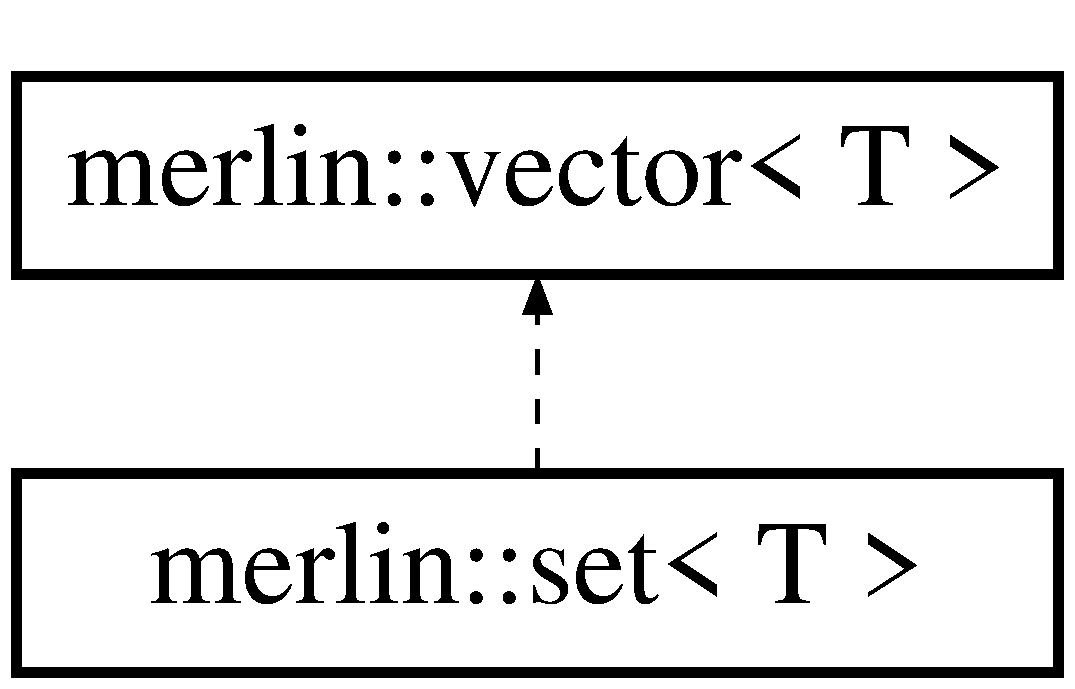
\includegraphics[height=2.000000cm]{classmerlin_1_1vector}
\end{center}
\end{figure}
\subsection*{Public Member Functions}
\begin{DoxyCompactItemize}
\item 
\hyperlink{classmerlin_1_1vector_ac48f70c583d3781dde90008b91a1b7a8}{vector} ()\hypertarget{classmerlin_1_1vector_ac48f70c583d3781dde90008b91a1b7a8}{}\label{classmerlin_1_1vector_ac48f70c583d3781dde90008b91a1b7a8}

\begin{DoxyCompactList}\small\item\em Construct empty vector. \end{DoxyCompactList}\item 
\hyperlink{classmerlin_1_1vector_a0e384bcf03c3f2886dedf1b24fc61057}{vector} (size\+\_\+t n, const T \&t=T())\hypertarget{classmerlin_1_1vector_a0e384bcf03c3f2886dedf1b24fc61057}{}\label{classmerlin_1_1vector_a0e384bcf03c3f2886dedf1b24fc61057}

\begin{DoxyCompactList}\small\item\em Construct vector with a given nuber of elements. \end{DoxyCompactList}\item 
\hyperlink{classmerlin_1_1vector_aebdbc7cbb94b53343d7a0b5059ea2e0f}{vector} (\hyperlink{classmerlin_1_1vector}{vector}$<$ T $>$ const \&v)
\begin{DoxyCompactList}\small\item\em Copy constructor. \end{DoxyCompactList}\item 
{\footnotesize template$<$class in\+Iter $>$ }\\\hyperlink{classmerlin_1_1vector_a7af3ec7e6c6a760d277ed21479ee7500}{vector} (in\+Iter first, in\+Iter last)\hypertarget{classmerlin_1_1vector_a7af3ec7e6c6a760d277ed21479ee7500}{}\label{classmerlin_1_1vector_a7af3ec7e6c6a760d277ed21479ee7500}

\begin{DoxyCompactList}\small\item\em Construct vector from input iterators. \end{DoxyCompactList}\item 
\hyperlink{classmerlin_1_1vector}{vector}$<$ T $>$ \& \hyperlink{classmerlin_1_1vector_a0f114ae4ee7406d5ba5d48b326fc3173}{operator=} (const \hyperlink{classmerlin_1_1vector}{vector}$<$ T $>$ \&v)
\begin{DoxyCompactList}\small\item\em Assign content. \end{DoxyCompactList}\item 
bool \hyperlink{classmerlin_1_1vector_a8def264e9a1d31a332ceb587f58f0306}{operator==} (const \hyperlink{classmerlin_1_1vector}{vector}$<$ T $>$ \&t) const \hypertarget{classmerlin_1_1vector_a8def264e9a1d31a332ceb587f58f0306}{}\label{classmerlin_1_1vector_a8def264e9a1d31a332ceb587f58f0306}

\begin{DoxyCompactList}\small\item\em Equality operator under lexicographical order. \end{DoxyCompactList}\item 
bool \hyperlink{classmerlin_1_1vector_a94d39609027858a133eea259ea1818ce}{operator!=} (const \hyperlink{classmerlin_1_1vector}{vector}$<$ T $>$ \&t) const \hypertarget{classmerlin_1_1vector_a94d39609027858a133eea259ea1818ce}{}\label{classmerlin_1_1vector_a94d39609027858a133eea259ea1818ce}

\begin{DoxyCompactList}\small\item\em Not-\/equal operator under lexicographical order. \end{DoxyCompactList}\item 
bool \hyperlink{classmerlin_1_1vector_a183cae0303276e9c310ce383fa67a126}{operator$<$} (const \hyperlink{classmerlin_1_1vector}{vector}$<$ T $>$ \&t) const \hypertarget{classmerlin_1_1vector_a183cae0303276e9c310ce383fa67a126}{}\label{classmerlin_1_1vector_a183cae0303276e9c310ce383fa67a126}

\begin{DoxyCompactList}\small\item\em Less-\/than operator under lexicographical order. \end{DoxyCompactList}\item 
bool \hyperlink{classmerlin_1_1vector_a0bf2c3e70321a5ed17036762513afebd}{operator$<$=} (const \hyperlink{classmerlin_1_1vector}{vector}$<$ T $>$ \&t) const \hypertarget{classmerlin_1_1vector_a0bf2c3e70321a5ed17036762513afebd}{}\label{classmerlin_1_1vector_a0bf2c3e70321a5ed17036762513afebd}

\begin{DoxyCompactList}\small\item\em Less-\/or-\/equal-\/than operator under lexicographical order. \end{DoxyCompactList}\item 
bool \hyperlink{classmerlin_1_1vector_a064996c92138178f03fd9147cd382122}{operator$>$} (const \hyperlink{classmerlin_1_1vector}{vector}$<$ T $>$ \&t) const \hypertarget{classmerlin_1_1vector_a064996c92138178f03fd9147cd382122}{}\label{classmerlin_1_1vector_a064996c92138178f03fd9147cd382122}

\begin{DoxyCompactList}\small\item\em Greater-\/than operator under lexicographical order. \end{DoxyCompactList}\item 
bool \hyperlink{classmerlin_1_1vector_a83dbba1136d7ed0af355b01b89de8d65}{operator$>$=} (const \hyperlink{classmerlin_1_1vector}{vector}$<$ T $>$ \&t) const \hypertarget{classmerlin_1_1vector_a83dbba1136d7ed0af355b01b89de8d65}{}\label{classmerlin_1_1vector_a83dbba1136d7ed0af355b01b89de8d65}

\begin{DoxyCompactList}\small\item\em Greater-\/or-\/equal-\/than operator under lexicographical order. \end{DoxyCompactList}\end{DoxyCompactItemize}
\subsection*{Protected Member Functions}
\begin{DoxyCompactItemize}
\item 
void \hyperlink{classmerlin_1_1vector_aa028c7af6c1149967f36241fa8b17d6c}{update} (void)\hypertarget{classmerlin_1_1vector_aa028c7af6c1149967f36241fa8b17d6c}{}\label{classmerlin_1_1vector_aa028c7af6c1149967f36241fa8b17d6c}

\begin{DoxyCompactList}\small\item\em Update the size of container. \end{DoxyCompactList}\end{DoxyCompactItemize}
\subsection*{Protected Attributes}
\begin{DoxyCompactItemize}
\item 
size\+\_\+t \hyperlink{classmerlin_1_1vector_a1e8ed92fa4fd93cd512e6ef59fbbf704}{m\+\_\+n}\hypertarget{classmerlin_1_1vector_a1e8ed92fa4fd93cd512e6ef59fbbf704}{}\label{classmerlin_1_1vector_a1e8ed92fa4fd93cd512e6ef59fbbf704}

\begin{DoxyCompactList}\small\item\em Number of elements. \end{DoxyCompactList}\end{DoxyCompactItemize}


\subsection{Detailed Description}
\subsubsection*{template$<$class T$>$\\*
class merlin\+::vector$<$ T $>$}

Container representing an array that can change in size. 

Definition at line 46 of file vector.\+h.



\subsection{Constructor \& Destructor Documentation}
\index{merlin\+::vector@{merlin\+::vector}!vector@{vector}}
\index{vector@{vector}!merlin\+::vector@{merlin\+::vector}}
\subsubsection[{\texorpdfstring{vector(vector$<$ T $>$ const \&v)}{vector(vector< T > const &v)}}]{\setlength{\rightskip}{0pt plus 5cm}template$<$class T$>$ {\bf merlin\+::vector}$<$ T $>$\+::{\bf vector} (
\begin{DoxyParamCaption}
\item[{{\bf vector}$<$ T $>$ const \&}]{v}
\end{DoxyParamCaption}
)\hspace{0.3cm}{\ttfamily [inline]}}\hypertarget{classmerlin_1_1vector_aebdbc7cbb94b53343d7a0b5059ea2e0f}{}\label{classmerlin_1_1vector_aebdbc7cbb94b53343d7a0b5059ea2e0f}


Copy constructor. 


\begin{DoxyParams}{Parameters}
{\em v} & A vector object of the same type. \\
\hline
\end{DoxyParams}


Definition at line 71 of file vector.\+h.



\subsection{Member Function Documentation}
\index{merlin\+::vector@{merlin\+::vector}!operator=@{operator=}}
\index{operator=@{operator=}!merlin\+::vector@{merlin\+::vector}}
\subsubsection[{\texorpdfstring{operator=(const vector$<$ T $>$ \&v)}{operator=(const vector< T > &v)}}]{\setlength{\rightskip}{0pt plus 5cm}template$<$class T$>$ {\bf vector}$<$T$>$\& {\bf merlin\+::vector}$<$ T $>$\+::operator= (
\begin{DoxyParamCaption}
\item[{const {\bf vector}$<$ T $>$ \&}]{v}
\end{DoxyParamCaption}
)\hspace{0.3cm}{\ttfamily [inline]}}\hypertarget{classmerlin_1_1vector_a0f114ae4ee7406d5ba5d48b326fc3173}{}\label{classmerlin_1_1vector_a0f114ae4ee7406d5ba5d48b326fc3173}


Assign content. 


\begin{DoxyParams}{Parameters}
{\em v} & A vector object of the same type. \\
\hline
\end{DoxyParams}


Definition at line 85 of file vector.\+h.



Referenced by merlin\+::set$<$ T $>$\+::operator=(), and merlin\+::set$<$ T $>$\+::set().



The documentation for this class was generated from the following file\+:\begin{DoxyCompactItemize}
\item 
src/include/\hyperlink{vector_8h}{vector.\+h}\end{DoxyCompactItemize}

\hypertarget{classmerlin_1_1wmb}{}\section{merlin\+:\+:wmb Class Reference}
\label{classmerlin_1_1wmb}\index{merlin\+::wmb@{merlin\+::wmb}}


{\ttfamily \#include $<$wmb.\+h$>$}

Inheritance diagram for merlin\+:\+:wmb\+:\begin{figure}[H]
\begin{center}
\leavevmode
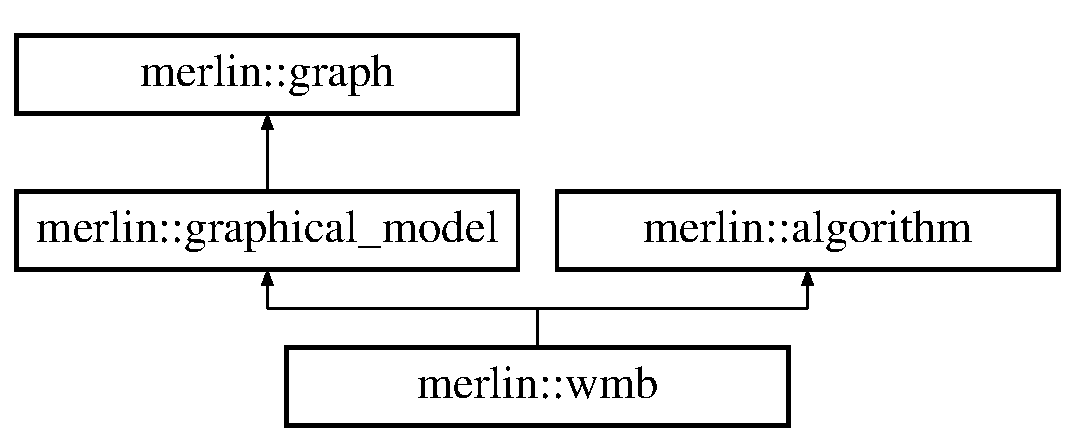
\includegraphics[height=3.000000cm]{classmerlin_1_1wmb}
\end{center}
\end{figure}
\subsection*{Classes}
\begin{DoxyCompactItemize}
\item 
struct \hyperlink{structmerlin_1_1wmb_1_1Pair}{Pair}
\begin{DoxyCompactList}\small\item\em Helper class for pairs of sorted indices. \end{DoxyCompactList}\end{DoxyCompactItemize}
\subsection*{Public Types}
\begin{DoxyCompactItemize}
\item 
typedef \hyperlink{classmerlin_1_1graphical__model_ab2b46f09d8142bb68f243ecadbdabb6b}{graphical\+\_\+model\+::findex} \hyperlink{classmerlin_1_1wmb_a5b845e1e9c8b169094995a385abb232a}{findex}\hypertarget{classmerlin_1_1wmb_a5b845e1e9c8b169094995a385abb232a}{}\label{classmerlin_1_1wmb_a5b845e1e9c8b169094995a385abb232a}

\begin{DoxyCompactList}\small\item\em Factor index. \end{DoxyCompactList}\item 
typedef \hyperlink{classmerlin_1_1graphical__model_a275006a490bc09239c12a4d93d53b135}{graphical\+\_\+model\+::vindex} \hyperlink{classmerlin_1_1wmb_ab942720d1c65e0002674af4eeade660f}{vindex}\hypertarget{classmerlin_1_1wmb_ab942720d1c65e0002674af4eeade660f}{}\label{classmerlin_1_1wmb_ab942720d1c65e0002674af4eeade660f}

\begin{DoxyCompactList}\small\item\em Variable index. \end{DoxyCompactList}\item 
typedef \hyperlink{classmerlin_1_1graphical__model_a615e25ec6594615fddfd4c3c4776b99f}{graphical\+\_\+model\+::flist} \hyperlink{classmerlin_1_1wmb_a7bb6da64d2971a1b46471b1898ff4efd}{flist}\hypertarget{classmerlin_1_1wmb_a7bb6da64d2971a1b46471b1898ff4efd}{}\label{classmerlin_1_1wmb_a7bb6da64d2971a1b46471b1898ff4efd}

\begin{DoxyCompactList}\small\item\em Collection of factor indices. \end{DoxyCompactList}\end{DoxyCompactItemize}
\subsection*{Public Member Functions}
\begin{DoxyCompactItemize}
\item 
\hyperlink{classmerlin_1_1wmb_ad0c30c53e9d8bbeda74d8d31f62107a9}{wmb} ()\hypertarget{classmerlin_1_1wmb_ad0c30c53e9d8bbeda74d8d31f62107a9}{}\label{classmerlin_1_1wmb_ad0c30c53e9d8bbeda74d8d31f62107a9}

\begin{DoxyCompactList}\small\item\em Default constructor. \end{DoxyCompactList}\item 
\hyperlink{classmerlin_1_1wmb_abef767965df7df0ac02ec38ca531dccd}{wmb} (const \hyperlink{classmerlin_1_1graphical__model}{graphical\+\_\+model} \&gm)\hypertarget{classmerlin_1_1wmb_abef767965df7df0ac02ec38ca531dccd}{}\label{classmerlin_1_1wmb_abef767965df7df0ac02ec38ca531dccd}

\begin{DoxyCompactList}\small\item\em Constructor with a graphical model. \end{DoxyCompactList}\item 
virtual \hyperlink{classmerlin_1_1wmb}{wmb} $\ast$ \hyperlink{classmerlin_1_1wmb_a9a9120ce51df90d8c6fc60c01f308dd4}{clone} () const 
\begin{DoxyCompactList}\small\item\em Clone the algorithm. \end{DoxyCompactList}\item 
double \hyperlink{classmerlin_1_1wmb_a78d08bbf18835324d79a4f73eebeecc7}{ub} () const 
\begin{DoxyCompactList}\small\item\em Upper bound on the optimal value. \end{DoxyCompactList}\item 
double \hyperlink{classmerlin_1_1wmb_a88a812b53de1bde731d7d21305be6041}{lb} () const 
\begin{DoxyCompactList}\small\item\em Lower bound on the optimal value. \end{DoxyCompactList}\item 
std\+::vector$<$ size\+\_\+t $>$ \hyperlink{classmerlin_1_1wmb_ae2de6f3bc30e524b6e9190d02631af4f}{best\+\_\+config} () const 
\begin{DoxyCompactList}\small\item\em Best configuration. \end{DoxyCompactList}\item 
double \hyperlink{classmerlin_1_1wmb_aa2af3a4102ee07f954d24c44066f6a08}{logZ} () const 
\begin{DoxyCompactList}\small\item\em Log value of the partition function. \end{DoxyCompactList}\item 
double \hyperlink{classmerlin_1_1wmb_a91015e29caed663c30bb37cbd0609e24}{log\+Zub} () const 
\begin{DoxyCompactList}\small\item\em Upper bound on the log partition function. \end{DoxyCompactList}\item 
double \hyperlink{classmerlin_1_1wmb_affa03e963d632f43e2c5967cd3f7bff4}{log\+Zlb} () const 
\begin{DoxyCompactList}\small\item\em Lower bound on the log partition function. \end{DoxyCompactList}\item 
const \hyperlink{classmerlin_1_1factor}{factor} \& \hyperlink{classmerlin_1_1wmb_aeb4e3096861b442f85ad8d1344172d18}{belief} (size\+\_\+t f) const 
\begin{DoxyCompactList}\small\item\em Belief associated with a node of the graph. \end{DoxyCompactList}\item 
const \hyperlink{classmerlin_1_1factor}{factor} \& \hyperlink{classmerlin_1_1wmb_a93588ec46d0cc1e54179ce8555862941}{belief} (\hyperlink{classmerlin_1_1variable}{variable} v) const 
\begin{DoxyCompactList}\small\item\em Belief associated with a particular variable. \end{DoxyCompactList}\item 
const \hyperlink{classmerlin_1_1factor}{factor} \& \hyperlink{classmerlin_1_1wmb_afe50fb8a9334a9f8b4653a75f20abd30}{belief} (\hyperlink{classmerlin_1_1variable__set}{variable\+\_\+set} vs) const 
\begin{DoxyCompactList}\small\item\em Belief associated with a set of variables. \end{DoxyCompactList}\item 
const \hyperlink{classmerlin_1_1vector}{vector}$<$ \hyperlink{classmerlin_1_1factor}{factor} $>$ \& \hyperlink{classmerlin_1_1wmb_ab433dc54ee1777fa163af30aa71bde3d}{beliefs} () const 
\begin{DoxyCompactList}\small\item\em Beliefs associated with the variables. \end{DoxyCompactList}\item 
const \hyperlink{classmerlin_1_1graphical__model}{graphical\+\_\+model} \& \hyperlink{classmerlin_1_1wmb_a5060018ee2950dac945e4efcb21a36d1}{get\+\_\+gm\+\_\+orig} () const \hypertarget{classmerlin_1_1wmb_a5060018ee2950dac945e4efcb21a36d1}{}\label{classmerlin_1_1wmb_a5060018ee2950dac945e4efcb21a36d1}

\begin{DoxyCompactList}\small\item\em Get the original graphical model. \end{DoxyCompactList}\item 
void \hyperlink{classmerlin_1_1wmb_adfc9d5e1b077918f71c17f8b0e56a13a}{write\+\_\+solution} (const char $\ast$file\+\_\+name, const std\+::map$<$ size\+\_\+t, size\+\_\+t $>$ \&evidence, const std\+::map$<$ size\+\_\+t, size\+\_\+t $>$ \&old2new, const \hyperlink{classmerlin_1_1graphical__model}{graphical\+\_\+model} \&orig, const bool first=true)
\begin{DoxyCompactList}\small\item\em Write the solution to the output file. \end{DoxyCompactList}\item 
virtual void \hyperlink{classmerlin_1_1wmb_acdbdfbded7a99152f8e7215c57cf1ab5}{run} ()\hypertarget{classmerlin_1_1wmb_acdbdfbded7a99152f8e7215c57cf1ab5}{}\label{classmerlin_1_1wmb_acdbdfbded7a99152f8e7215c57cf1ab5}

\begin{DoxyCompactList}\small\item\em Run the weighted mini-\/buckets algorithm. \end{DoxyCompactList}\item 
\hyperlink{classmerlin_1_1wmb_af800e4c2c35e845cc47bab94ef156aac}{M\+E\+R\+\_\+\+E\+N\+UM} (Task, PR, M\+AR, M\+AP, M\+M\+AP)\hypertarget{classmerlin_1_1wmb_af800e4c2c35e845cc47bab94ef156aac}{}\label{classmerlin_1_1wmb_af800e4c2c35e845cc47bab94ef156aac}

\begin{DoxyCompactList}\small\item\em Inference tasks supported. \end{DoxyCompactList}\item 
\hyperlink{classmerlin_1_1wmb_add42202a2c38f0a65f1de8ddcbbb08f8}{M\+E\+R\+\_\+\+E\+N\+UM} (Property, i\+Bound, Order, Task, Iter, Debug, Order\+Iter)\hypertarget{classmerlin_1_1wmb_add42202a2c38f0a65f1de8ddcbbb08f8}{}\label{classmerlin_1_1wmb_add42202a2c38f0a65f1de8ddcbbb08f8}

\begin{DoxyCompactList}\small\item\em Properties of the algorithm. \end{DoxyCompactList}\item 
void \hyperlink{classmerlin_1_1wmb_a0d1389be67caece79708d4914ff03185}{set\+\_\+ibound} (size\+\_\+t i)\hypertarget{classmerlin_1_1wmb_a0d1389be67caece79708d4914ff03185}{}\label{classmerlin_1_1wmb_a0d1389be67caece79708d4914ff03185}

\begin{DoxyCompactList}\small\item\em Set the mini-\/bucket i-\/bound parameter. \end{DoxyCompactList}\item 
size\+\_\+t \hyperlink{classmerlin_1_1wmb_ae625b40db68f51aadb954da99e48bc52}{get\+\_\+ibound} () const \hypertarget{classmerlin_1_1wmb_ae625b40db68f51aadb954da99e48bc52}{}\label{classmerlin_1_1wmb_ae625b40db68f51aadb954da99e48bc52}

\begin{DoxyCompactList}\small\item\em Get the mini-\/bucket i-\/bound parameter. \end{DoxyCompactList}\item 
void \hyperlink{classmerlin_1_1wmb_a0dcda9d7c557d77435aa0363e793018e}{set\+\_\+var\+\_\+types} (const \hyperlink{classmerlin_1_1vector}{vector}$<$ bool $>$ \&var\+\_\+types)\hypertarget{classmerlin_1_1wmb_a0dcda9d7c557d77435aa0363e793018e}{}\label{classmerlin_1_1wmb_a0dcda9d7c557d77435aa0363e793018e}

\begin{DoxyCompactList}\small\item\em Set the variable types. \end{DoxyCompactList}\item 
const \hyperlink{classmerlin_1_1vector}{vector}$<$ bool $>$ \& \hyperlink{classmerlin_1_1wmb_a6bd57e3e3351407403d7cdf619ea286b}{get\+\_\+var\+\_\+types} () const \hypertarget{classmerlin_1_1wmb_a6bd57e3e3351407403d7cdf619ea286b}{}\label{classmerlin_1_1wmb_a6bd57e3e3351407403d7cdf619ea286b}

\begin{DoxyCompactList}\small\item\em Get the variable types. \end{DoxyCompactList}\item 
void \hyperlink{classmerlin_1_1wmb_aa16d549dcec0debda59998b3a8960212}{set\+\_\+order} (const variable\+\_\+order\+\_\+t \&ord)\hypertarget{classmerlin_1_1wmb_aa16d549dcec0debda59998b3a8960212}{}\label{classmerlin_1_1wmb_aa16d549dcec0debda59998b3a8960212}

\begin{DoxyCompactList}\small\item\em Set the variable order. \end{DoxyCompactList}\item 
void \hyperlink{classmerlin_1_1wmb_a4d6c6775868cac1a8559be5575d301f5}{set\+\_\+order\+\_\+method} (graphical\+\_\+model\+::\+Order\+Method method)\hypertarget{classmerlin_1_1wmb_a4d6c6775868cac1a8559be5575d301f5}{}\label{classmerlin_1_1wmb_a4d6c6775868cac1a8559be5575d301f5}

\begin{DoxyCompactList}\small\item\em Set the variable order method. \end{DoxyCompactList}\item 
const variable\+\_\+order\+\_\+t \& \hyperlink{classmerlin_1_1wmb_a2709605ec51725e4164d488bb71c81a7}{get\+\_\+order} ()\hypertarget{classmerlin_1_1wmb_a2709605ec51725e4164d488bb71c81a7}{}\label{classmerlin_1_1wmb_a2709605ec51725e4164d488bb71c81a7}

\begin{DoxyCompactList}\small\item\em Get the variable order. \end{DoxyCompactList}\item 
const std\+::vector$<$ \hyperlink{classmerlin_1_1wmb_ab942720d1c65e0002674af4eeade660f}{vindex} $>$ \& \hyperlink{classmerlin_1_1wmb_a23118e3df645be1029fa7642bf8fe090}{get\+\_\+pseudo\+\_\+tree} ()\hypertarget{classmerlin_1_1wmb_a23118e3df645be1029fa7642bf8fe090}{}\label{classmerlin_1_1wmb_a23118e3df645be1029fa7642bf8fe090}

\begin{DoxyCompactList}\small\item\em Get the pseudo tree. \end{DoxyCompactList}\item 
void \hyperlink{classmerlin_1_1wmb_a44f662696a361d292f0b0088487ed7a1}{set\+\_\+pseudo\+\_\+tree} (const \hyperlink{classmerlin_1_1vector}{vector}$<$ \hyperlink{classmerlin_1_1wmb_ab942720d1c65e0002674af4eeade660f}{vindex} $>$ \&p)\hypertarget{classmerlin_1_1wmb_a44f662696a361d292f0b0088487ed7a1}{}\label{classmerlin_1_1wmb_a44f662696a361d292f0b0088487ed7a1}

\begin{DoxyCompactList}\small\item\em Set the pseudo tree. \end{DoxyCompactList}\item 
void \hyperlink{classmerlin_1_1wmb_ae17b4c453a873d89925776cfc0773b5d}{set\+\_\+query} (const std\+::vector$<$ \hyperlink{classmerlin_1_1wmb_ab942720d1c65e0002674af4eeade660f}{vindex} $>$ \&q)\hypertarget{classmerlin_1_1wmb_ae17b4c453a873d89925776cfc0773b5d}{}\label{classmerlin_1_1wmb_ae17b4c453a873d89925776cfc0773b5d}

\begin{DoxyCompactList}\small\item\em Set the query (M\+AP) variables. \end{DoxyCompactList}\item 
const std\+::vector$<$ \hyperlink{classmerlin_1_1wmb_ab942720d1c65e0002674af4eeade660f}{vindex} $>$ \& \hyperlink{classmerlin_1_1wmb_a1ff63d89f0dd759ab184712335396393}{get\+\_\+query} ()\hypertarget{classmerlin_1_1wmb_a1ff63d89f0dd759ab184712335396393}{}\label{classmerlin_1_1wmb_a1ff63d89f0dd759ab184712335396393}

\begin{DoxyCompactList}\small\item\em Get the query (M\+AP) variables. \end{DoxyCompactList}\item 
void \hyperlink{classmerlin_1_1wmb_a8308f0c51a3f354e66d38f6639eebadf}{set\+\_\+graphical\+\_\+model} (const \hyperlink{classmerlin_1_1graphical__model}{graphical\+\_\+model} \&gm)\hypertarget{classmerlin_1_1wmb_a8308f0c51a3f354e66d38f6639eebadf}{}\label{classmerlin_1_1wmb_a8308f0c51a3f354e66d38f6639eebadf}

\begin{DoxyCompactList}\small\item\em Set the graphical model. \end{DoxyCompactList}\item 
void \hyperlink{classmerlin_1_1wmb_a5d4249884de8c97b00a5a58ce9b18c56}{set\+\_\+graphical\+\_\+model} (const \hyperlink{classmerlin_1_1vector}{vector}$<$ \hyperlink{classmerlin_1_1factor}{factor} $>$ \&fs)\hypertarget{classmerlin_1_1wmb_a5d4249884de8c97b00a5a58ce9b18c56}{}\label{classmerlin_1_1wmb_a5d4249884de8c97b00a5a58ce9b18c56}

\begin{DoxyCompactList}\small\item\em Set the graphical model from a list of factors. \end{DoxyCompactList}\item 
virtual void \hyperlink{classmerlin_1_1wmb_aa8868851a3f7c8d1c43326f431bd1132}{set\+\_\+properties} (std\+::string opt=std\+::string())
\begin{DoxyCompactList}\small\item\em Set the properties of the algorithm. \end{DoxyCompactList}\item 
\hyperlink{classmerlin_1_1factor}{factor} \hyperlink{classmerlin_1_1wmb_a9acbede3a21446ef005eaae637ec344e}{elim} (const \hyperlink{classmerlin_1_1factor}{factor} \&F, const \hyperlink{classmerlin_1_1variable__set}{variable\+\_\+set} \&vs, const double w)
\begin{DoxyCompactList}\small\item\em Eliminate a set of variables from a factor. \end{DoxyCompactList}\item 
\hyperlink{classmerlin_1_1factor}{factor} \hyperlink{classmerlin_1_1wmb_a6abd46dbb20aa12ef7b2bfa93cefc36d}{marg} (const \hyperlink{classmerlin_1_1factor}{factor} \&F, const \hyperlink{classmerlin_1_1variable__set}{variable\+\_\+set} \&vs, const double w)
\begin{DoxyCompactList}\small\item\em Compute the weighted marginal over a set of variables. \end{DoxyCompactList}\item 
double \hyperlink{classmerlin_1_1wmb_aa4cadd87c907327227427ba1f9555350}{score} (const \hyperlink{classmerlin_1_1vector}{vector}$<$ \hyperlink{classmerlin_1_1variable__set}{variable\+\_\+set} $>$ \&fin, const \hyperlink{classmerlin_1_1variable}{variable} \&VX, size\+\_\+t i, size\+\_\+t j)
\begin{DoxyCompactList}\small\item\em Scoring function for bucket aggregation. \end{DoxyCompactList}\item 
void \hyperlink{classmerlin_1_1wmb_ac9a83bcbef3f06a48d6cd9bea8ad3ce6}{init} ()\hypertarget{classmerlin_1_1wmb_ac9a83bcbef3f06a48d6cd9bea8ad3ce6}{}\label{classmerlin_1_1wmb_ac9a83bcbef3f06a48d6cd9bea8ad3ce6}

\begin{DoxyCompactList}\small\item\em Initialize the weighted mini-\/buckets algorithm. \end{DoxyCompactList}\item 
\hyperlink{classmerlin_1_1factor}{factor} \hyperlink{classmerlin_1_1wmb_a67bd322cf76dd18439123f244c8e95d9}{calc\+\_\+belief} (\hyperlink{classmerlin_1_1wmb_a5b845e1e9c8b169094995a385abb232a}{findex} a)
\begin{DoxyCompactList}\small\item\em Compute the belief of a cluster. \end{DoxyCompactList}\item 
\hyperlink{classmerlin_1_1factor}{factor} \hyperlink{classmerlin_1_1wmb_ad79e4290a7a13c13ba249d764704090a}{incoming} (\hyperlink{classmerlin_1_1wmb_a5b845e1e9c8b169094995a385abb232a}{findex} a, size\+\_\+t i)
\begin{DoxyCompactList}\small\item\em Compute the belief of a cluster excluding an incoming message. \end{DoxyCompactList}\item 
\hyperlink{classmerlin_1_1factor}{factor} \hyperlink{classmerlin_1_1wmb_af49cff26f827f40b710f06f9ebc6e01e}{incoming} (\hyperlink{classmerlin_1_1wmb_a5b845e1e9c8b169094995a385abb232a}{findex} a)
\begin{DoxyCompactList}\small\item\em Compute the belief of a cluster excluding backward messages. \end{DoxyCompactList}\item 
void \hyperlink{classmerlin_1_1wmb_ae0751c60569981427b9aea293e7ae6ba}{forward} (double step)\hypertarget{classmerlin_1_1wmb_ae0751c60569981427b9aea293e7ae6ba}{}\label{classmerlin_1_1wmb_ae0751c60569981427b9aea293e7ae6ba}

\begin{DoxyCompactList}\small\item\em Forward (top-\/down) message passing with moment matching between the clusters of a bucket. \end{DoxyCompactList}\item 
void \hyperlink{classmerlin_1_1wmb_af70144800198fa62226da1cc94b8a932}{backward} (size\+\_\+t iter)\hypertarget{classmerlin_1_1wmb_af70144800198fa62226da1cc94b8a932}{}\label{classmerlin_1_1wmb_af70144800198fa62226da1cc94b8a932}

\begin{DoxyCompactList}\small\item\em Backward (bottom-\/up) message passing. \end{DoxyCompactList}\item 
void \hyperlink{classmerlin_1_1wmb_a15f2962a5be2bff5c8778018c8dc785d}{match\+\_\+clusters} (size\+\_\+t x, double step)\hypertarget{classmerlin_1_1wmb_a15f2962a5be2bff5c8778018c8dc785d}{}\label{classmerlin_1_1wmb_a15f2962a5be2bff5c8778018c8dc785d}

\begin{DoxyCompactList}\small\item\em Perform moment-\/matching between the clusters of a variable. \end{DoxyCompactList}\item 
void \hyperlink{classmerlin_1_1wmb_a5ef13c682161de26ab1f89b3719e69e3}{tighten} (size\+\_\+t n\+Iter, double stop\+Time=-\/1, double stop\+Obj=-\/1)\hypertarget{classmerlin_1_1wmb_a5ef13c682161de26ab1f89b3719e69e3}{}\label{classmerlin_1_1wmb_a5ef13c682161de26ab1f89b3719e69e3}

\begin{DoxyCompactList}\small\item\em Iterative tightening of the upper bound. \end{DoxyCompactList}\item 
void \hyperlink{classmerlin_1_1wmb_a761421a2ad5cd8bcba09a69b7e9713a6}{update} ()\hypertarget{classmerlin_1_1wmb_a761421a2ad5cd8bcba09a69b7e9713a6}{}\label{classmerlin_1_1wmb_a761421a2ad5cd8bcba09a69b7e9713a6}

\begin{DoxyCompactList}\small\item\em Update the beliefs (marginals or max-\/marginals) \end{DoxyCompactList}\end{DoxyCompactItemize}
\subsection*{Protected Attributes}
\begin{DoxyCompactItemize}
\item 
\hyperlink{classmerlin_1_1graphical__model}{graphical\+\_\+model} \hyperlink{classmerlin_1_1wmb_a3aaf9e90947e65689d112c165f734b40}{m\+\_\+gmo}\hypertarget{classmerlin_1_1wmb_a3aaf9e90947e65689d112c165f734b40}{}\label{classmerlin_1_1wmb_a3aaf9e90947e65689d112c165f734b40}

\begin{DoxyCompactList}\small\item\em Original graphical model. \end{DoxyCompactList}\item 
Task \hyperlink{classmerlin_1_1wmb_ae015453f4b405e1ab4798d32a09fe63d}{m\+\_\+task}\hypertarget{classmerlin_1_1wmb_ae015453f4b405e1ab4798d32a09fe63d}{}\label{classmerlin_1_1wmb_ae015453f4b405e1ab4798d32a09fe63d}

\begin{DoxyCompactList}\small\item\em Inference task. \end{DoxyCompactList}\item 
Order\+Method \hyperlink{classmerlin_1_1wmb_ac9c473f2f6c6f727bc694a1ecb3cec16}{m\+\_\+order\+\_\+method}\hypertarget{classmerlin_1_1wmb_ac9c473f2f6c6f727bc694a1ecb3cec16}{}\label{classmerlin_1_1wmb_ac9c473f2f6c6f727bc694a1ecb3cec16}

\begin{DoxyCompactList}\small\item\em Variable ordering method. \end{DoxyCompactList}\item 
size\+\_\+t \hyperlink{classmerlin_1_1wmb_a56b67b58895055abf6e881a9ae3237c0}{m\+\_\+order\+\_\+iter}\hypertarget{classmerlin_1_1wmb_a56b67b58895055abf6e881a9ae3237c0}{}\label{classmerlin_1_1wmb_a56b67b58895055abf6e881a9ae3237c0}

\begin{DoxyCompactList}\small\item\em Number of iterations for ordering heuristic. \end{DoxyCompactList}\item 
size\+\_\+t \hyperlink{classmerlin_1_1wmb_a56f63e7abb2345db6cba7bb0a6572386}{m\+\_\+ibound}\hypertarget{classmerlin_1_1wmb_a56f63e7abb2345db6cba7bb0a6572386}{}\label{classmerlin_1_1wmb_a56f63e7abb2345db6cba7bb0a6572386}

\begin{DoxyCompactList}\small\item\em Mini-\/bucket i-\/bound. \end{DoxyCompactList}\item 
double \hyperlink{classmerlin_1_1wmb_ac0e420613dd6b983ade039b5c0951bf2}{m\+\_\+log\+\_\+z}\hypertarget{classmerlin_1_1wmb_ac0e420613dd6b983ade039b5c0951bf2}{}\label{classmerlin_1_1wmb_ac0e420613dd6b983ade039b5c0951bf2}

\begin{DoxyCompactList}\small\item\em Log partition function value. \end{DoxyCompactList}\item 
variable\+\_\+order\+\_\+t \hyperlink{classmerlin_1_1wmb_a90dcccb0c36b950773488d6571f63794}{m\+\_\+order}\hypertarget{classmerlin_1_1wmb_a90dcccb0c36b950773488d6571f63794}{}\label{classmerlin_1_1wmb_a90dcccb0c36b950773488d6571f63794}

\begin{DoxyCompactList}\small\item\em Variable order. \end{DoxyCompactList}\item 
std\+::vector$<$ \hyperlink{classmerlin_1_1wmb_ab942720d1c65e0002674af4eeade660f}{vindex} $>$ \hyperlink{classmerlin_1_1wmb_a5f61b40f731ee4bdd5925573dccb0d67}{m\+\_\+parents}\hypertarget{classmerlin_1_1wmb_a5f61b40f731ee4bdd5925573dccb0d67}{}\label{classmerlin_1_1wmb_a5f61b40f731ee4bdd5925573dccb0d67}

\begin{DoxyCompactList}\small\item\em Pseudo tree. \end{DoxyCompactList}\item 
\hyperlink{classmerlin_1_1vector}{vector}$<$ bool $>$ \hyperlink{classmerlin_1_1wmb_a3168b866bd967a777a37d5e48a360452}{m\+\_\+var\+\_\+types}\hypertarget{classmerlin_1_1wmb_a3168b866bd967a777a37d5e48a360452}{}\label{classmerlin_1_1wmb_a3168b866bd967a777a37d5e48a360452}

\begin{DoxyCompactList}\small\item\em Variable types (true if M\+AX, false if S\+UM) \end{DoxyCompactList}\item 
\hyperlink{classmerlin_1_1vector}{vector}$<$ \hyperlink{classmerlin_1_1factor}{factor} $>$ \hyperlink{classmerlin_1_1wmb_a0ddbaa2a79b9d8b06f58b9f476250fd2}{m\+\_\+beliefs}\hypertarget{classmerlin_1_1wmb_a0ddbaa2a79b9d8b06f58b9f476250fd2}{}\label{classmerlin_1_1wmb_a0ddbaa2a79b9d8b06f58b9f476250fd2}

\begin{DoxyCompactList}\small\item\em Marginals. \end{DoxyCompactList}\item 
std\+::vector$<$ \hyperlink{classmerlin_1_1wmb_ab942720d1c65e0002674af4eeade660f}{vindex} $>$ \hyperlink{classmerlin_1_1wmb_a0f74574e4a8fe116fb2c8cac3133285c}{m\+\_\+best\+\_\+config}\hypertarget{classmerlin_1_1wmb_a0f74574e4a8fe116fb2c8cac3133285c}{}\label{classmerlin_1_1wmb_a0f74574e4a8fe116fb2c8cac3133285c}

\begin{DoxyCompactList}\small\item\em M\+AP assignment. \end{DoxyCompactList}\item 
std\+::vector$<$ \hyperlink{classmerlin_1_1wmb_ab942720d1c65e0002674af4eeade660f}{vindex} $>$ \hyperlink{classmerlin_1_1wmb_a371fef243f301501c4c4ab66110d6e4f}{m\+\_\+query}\hypertarget{classmerlin_1_1wmb_a371fef243f301501c4c4ab66110d6e4f}{}\label{classmerlin_1_1wmb_a371fef243f301501c4c4ab66110d6e4f}

\begin{DoxyCompactList}\small\item\em M\+AX variables for the M\+M\+AP task. \end{DoxyCompactList}\item 
size\+\_\+t \hyperlink{classmerlin_1_1wmb_a743ab793f808e44b021f7e811df3521b}{m\+\_\+num\+\_\+iter}\hypertarget{classmerlin_1_1wmb_a743ab793f808e44b021f7e811df3521b}{}\label{classmerlin_1_1wmb_a743ab793f808e44b021f7e811df3521b}

\begin{DoxyCompactList}\small\item\em Number of iterations to be executed. \end{DoxyCompactList}\item 
double \hyperlink{classmerlin_1_1wmb_a68bc2a7e87eeab1021bf1877a3b200c6}{m\+\_\+lb}\hypertarget{classmerlin_1_1wmb_a68bc2a7e87eeab1021bf1877a3b200c6}{}\label{classmerlin_1_1wmb_a68bc2a7e87eeab1021bf1877a3b200c6}

\begin{DoxyCompactList}\small\item\em Lower bound (ie, value of M\+AP assignment) \end{DoxyCompactList}\end{DoxyCompactItemize}
\subsection*{Additional Inherited Members}


\subsection{Detailed Description}
Weighted Mini-\/\+Buckets (W\+MB)

Tasks supported\+: PR, M\+AR, M\+AP, M\+M\+AP

W\+MB generalizes the classical M\+BE by replacing the sum operator with a weighted sum operator, and thus it uses Holder\textquotesingle{}s inequality to derive an upper bound on the log partition function, M\+AP or Marginal M\+AP value. W\+MB also uses an iterative cost-\/shifting scheme that matches marginals (weighted or max) in order to tighten the upper-\/bound. Tightening is not guaranteed in general, but it typically happens in practice. 

Definition at line 46 of file wmb.\+h.



\subsection{Member Function Documentation}
\index{merlin\+::wmb@{merlin\+::wmb}!belief@{belief}}
\index{belief@{belief}!merlin\+::wmb@{merlin\+::wmb}}
\subsubsection[{\texorpdfstring{belief(size\+\_\+t f) const }{belief(size_t f) const }}]{\setlength{\rightskip}{0pt plus 5cm}const {\bf factor}\& merlin\+::wmb\+::belief (
\begin{DoxyParamCaption}
\item[{size\+\_\+t}]{i}
\end{DoxyParamCaption}
) const\hspace{0.3cm}{\ttfamily [inline]}, {\ttfamily [virtual]}}\hypertarget{classmerlin_1_1wmb_aeb4e3096861b442f85ad8d1344172d18}{}\label{classmerlin_1_1wmb_aeb4e3096861b442f85ad8d1344172d18}


Belief associated with a node of the graph. 

\begin{DoxyReturn}{Returns}
the belief associated with a node of the graph. Nodes correspond typically to variables. The belied is a function represented by the Factor class. 
\end{DoxyReturn}

\begin{DoxyParams}{Parameters}
{\em i} & The index of the node in the graph (from 0) \\
\hline
\end{DoxyParams}


Implements \hyperlink{classmerlin_1_1algorithm_a617b3e562037a7716f7cfd6cf1e55c19}{merlin\+::algorithm}.



Definition at line 100 of file wmb.\+h.



References m\+\_\+beliefs.



Referenced by run(), and write\+\_\+solution().

\index{merlin\+::wmb@{merlin\+::wmb}!belief@{belief}}
\index{belief@{belief}!merlin\+::wmb@{merlin\+::wmb}}
\subsubsection[{\texorpdfstring{belief(variable v) const }{belief(variable v) const }}]{\setlength{\rightskip}{0pt plus 5cm}const {\bf factor}\& merlin\+::wmb\+::belief (
\begin{DoxyParamCaption}
\item[{{\bf variable}}]{v}
\end{DoxyParamCaption}
) const\hspace{0.3cm}{\ttfamily [inline]}, {\ttfamily [virtual]}}\hypertarget{classmerlin_1_1wmb_a93588ec46d0cc1e54179ce8555862941}{}\label{classmerlin_1_1wmb_a93588ec46d0cc1e54179ce8555862941}


Belief associated with a particular variable. 


\begin{DoxyParams}{Parameters}
{\em v} & The variable to compute the belief of \\
\hline
\end{DoxyParams}
\begin{DoxyReturn}{Returns}
the belief associated with a particular variable in the graphical model. The belief is a function represented by the Factor class. 
\end{DoxyReturn}


Implements \hyperlink{classmerlin_1_1algorithm_adc966d1ed7ac479754441bab138f7efa}{merlin\+::algorithm}.



Definition at line 103 of file wmb.\+h.



References m\+\_\+beliefs.

\index{merlin\+::wmb@{merlin\+::wmb}!belief@{belief}}
\index{belief@{belief}!merlin\+::wmb@{merlin\+::wmb}}
\subsubsection[{\texorpdfstring{belief(variable\+\_\+set vs) const }{belief(variable_set vs) const }}]{\setlength{\rightskip}{0pt plus 5cm}const {\bf factor}\& merlin\+::wmb\+::belief (
\begin{DoxyParamCaption}
\item[{{\bf variable\+\_\+set}}]{vs}
\end{DoxyParamCaption}
) const\hspace{0.3cm}{\ttfamily [inline]}, {\ttfamily [virtual]}}\hypertarget{classmerlin_1_1wmb_afe50fb8a9334a9f8b4653a75f20abd30}{}\label{classmerlin_1_1wmb_afe50fb8a9334a9f8b4653a75f20abd30}


Belief associated with a set of variables. 


\begin{DoxyParams}{Parameters}
{\em vs} & The set of variables to compute the belief of \\
\hline
\end{DoxyParams}
\begin{DoxyReturn}{Returns}
the belief associated with a set of variables in the graphical model. The belief is a function represented by the Factor class. 
\end{DoxyReturn}


Implements \hyperlink{classmerlin_1_1algorithm_ad19b068623b85ad1cd4bb262e7bcfc6f}{merlin\+::algorithm}.



Definition at line 106 of file wmb.\+h.

\index{merlin\+::wmb@{merlin\+::wmb}!beliefs@{beliefs}}
\index{beliefs@{beliefs}!merlin\+::wmb@{merlin\+::wmb}}
\subsubsection[{\texorpdfstring{beliefs() const }{beliefs() const }}]{\setlength{\rightskip}{0pt plus 5cm}const {\bf vector}$<${\bf factor}$>$\& merlin\+::wmb\+::beliefs (
\begin{DoxyParamCaption}
{}
\end{DoxyParamCaption}
) const\hspace{0.3cm}{\ttfamily [inline]}, {\ttfamily [virtual]}}\hypertarget{classmerlin_1_1wmb_ab433dc54ee1777fa163af30aa71bde3d}{}\label{classmerlin_1_1wmb_ab433dc54ee1777fa163af30aa71bde3d}


Beliefs associated with the variables. 

\begin{DoxyReturn}{Returns}
the beliefs associated with the variables in the graphical model (one belief for each of the variables). The output vector is indexed by the same indexes used for the variables. 
\end{DoxyReturn}


Implements \hyperlink{classmerlin_1_1algorithm_a0b70d8fe87b32bca601a3d116b673b47}{merlin\+::algorithm}.



Definition at line 109 of file wmb.\+h.



References m\+\_\+beliefs.

\index{merlin\+::wmb@{merlin\+::wmb}!best\+\_\+config@{best\+\_\+config}}
\index{best\+\_\+config@{best\+\_\+config}!merlin\+::wmb@{merlin\+::wmb}}
\subsubsection[{\texorpdfstring{best\+\_\+config() const }{best_config() const }}]{\setlength{\rightskip}{0pt plus 5cm}std\+::vector$<$size\+\_\+t$>$ merlin\+::wmb\+::best\+\_\+config (
\begin{DoxyParamCaption}
{}
\end{DoxyParamCaption}
) const\hspace{0.3cm}{\ttfamily [inline]}, {\ttfamily [virtual]}}\hypertarget{classmerlin_1_1wmb_ae2de6f3bc30e524b6e9190d02631af4f}{}\label{classmerlin_1_1wmb_ae2de6f3bc30e524b6e9190d02631af4f}


Best configuration. 

\begin{DoxyReturn}{Returns}
a vector containing the best configuration of the variables (i.\+e., variable value assignments) found so far. It is specific to optimization tasks (e.\+g., M\+AP, Marginal M\+AP). 
\end{DoxyReturn}


Implements \hyperlink{classmerlin_1_1algorithm_a3d84d2595e6235db93a9bb3e1a012e48}{merlin\+::algorithm}.



Definition at line 85 of file wmb.\+h.



References m\+\_\+best\+\_\+config.

\index{merlin\+::wmb@{merlin\+::wmb}!calc\+\_\+belief@{calc\+\_\+belief}}
\index{calc\+\_\+belief@{calc\+\_\+belief}!merlin\+::wmb@{merlin\+::wmb}}
\subsubsection[{\texorpdfstring{calc\+\_\+belief(findex a)}{calc_belief(findex a)}}]{\setlength{\rightskip}{0pt plus 5cm}{\bf factor} merlin\+::wmb\+::calc\+\_\+belief (
\begin{DoxyParamCaption}
\item[{{\bf findex}}]{a}
\end{DoxyParamCaption}
)\hspace{0.3cm}{\ttfamily [inline]}}\hypertarget{classmerlin_1_1wmb_a67bd322cf76dd18439123f244c8e95d9}{}\label{classmerlin_1_1wmb_a67bd322cf76dd18439123f244c8e95d9}


Compute the belief of a cluster. 


\begin{DoxyParams}{Parameters}
{\em a} & The index of the cluster \\
\hline
\end{DoxyParams}
\begin{DoxyReturn}{Returns}
the factor representing the belief of the cluster. 
\end{DoxyReturn}


Definition at line 859 of file wmb.\+h.



References merlin\+::graphical\+\_\+model\+::m\+\_\+factors.



Referenced by backward(), forward(), match\+\_\+clusters(), and update().

\index{merlin\+::wmb@{merlin\+::wmb}!clone@{clone}}
\index{clone@{clone}!merlin\+::wmb@{merlin\+::wmb}}
\subsubsection[{\texorpdfstring{clone() const }{clone() const }}]{\setlength{\rightskip}{0pt plus 5cm}virtual {\bf wmb}$\ast$ merlin\+::wmb\+::clone (
\begin{DoxyParamCaption}
{}
\end{DoxyParamCaption}
) const\hspace{0.3cm}{\ttfamily [inline]}, {\ttfamily [virtual]}}\hypertarget{classmerlin_1_1wmb_a9a9120ce51df90d8c6fc60c01f308dd4}{}\label{classmerlin_1_1wmb_a9a9120ce51df90d8c6fc60c01f308dd4}


Clone the algorithm. 

\begin{DoxyReturn}{Returns}
the pointer to the new object containing the cloned algorithm. 
\end{DoxyReturn}


Implements \hyperlink{classmerlin_1_1algorithm_a10f787e24c1fd5ec92c26b18efb0b8db}{merlin\+::algorithm}.



Definition at line 73 of file wmb.\+h.



References wmb().

\index{merlin\+::wmb@{merlin\+::wmb}!elim@{elim}}
\index{elim@{elim}!merlin\+::wmb@{merlin\+::wmb}}
\subsubsection[{\texorpdfstring{elim(const factor \&\+F, const variable\+\_\+set \&vs, const double w)}{elim(const factor &F, const variable_set &vs, const double w)}}]{\setlength{\rightskip}{0pt plus 5cm}{\bf factor} merlin\+::wmb\+::elim (
\begin{DoxyParamCaption}
\item[{const {\bf factor} \&}]{F, }
\item[{const {\bf variable\+\_\+set} \&}]{vs, }
\item[{const double}]{w}
\end{DoxyParamCaption}
)\hspace{0.3cm}{\ttfamily [inline]}}\hypertarget{classmerlin_1_1wmb_a9acbede3a21446ef005eaae637ec344e}{}\label{classmerlin_1_1wmb_a9acbede3a21446ef005eaae637ec344e}


Eliminate a set of variables from a factor. 


\begin{DoxyParams}{Parameters}
{\em F} & The reference of the factor to eliminate from \\
\hline
{\em vs} & The set of variables to be eliminated \\
\hline
{\em w} & The weight of the weighted elimination operator \\
\hline
\end{DoxyParams}
\begin{DoxyReturn}{Returns}
the factor resulted from eliminating the set of variables. 
\end{DoxyReturn}


Definition at line 452 of file wmb.\+h.



References merlin\+::factor\+::sum\+\_\+power().

\index{merlin\+::wmb@{merlin\+::wmb}!incoming@{incoming}}
\index{incoming@{incoming}!merlin\+::wmb@{merlin\+::wmb}}
\subsubsection[{\texorpdfstring{incoming(findex a, size\+\_\+t i)}{incoming(findex a, size_t i)}}]{\setlength{\rightskip}{0pt plus 5cm}{\bf factor} merlin\+::wmb\+::incoming (
\begin{DoxyParamCaption}
\item[{{\bf findex}}]{a, }
\item[{size\+\_\+t}]{i}
\end{DoxyParamCaption}
)\hspace{0.3cm}{\ttfamily [inline]}}\hypertarget{classmerlin_1_1wmb_ad79e4290a7a13c13ba249d764704090a}{}\label{classmerlin_1_1wmb_ad79e4290a7a13c13ba249d764704090a}


Compute the belief of a cluster excluding an incoming message. 


\begin{DoxyParams}{Parameters}
{\em a} & The index of the cluster to compute the belief of \\
\hline
{\em i} & The index of the cluster sending the incoming message \\
\hline
\end{DoxyParams}
\begin{DoxyReturn}{Returns}
the factor representing the belief of cluster {\itshape a} excluding the incoming message from {\itshape i} to {\itshape a}. 
\end{DoxyReturn}


Definition at line 889 of file wmb.\+h.



References merlin\+::graphical\+\_\+model\+::m\+\_\+factors.



Referenced by forward(), and update().

\index{merlin\+::wmb@{merlin\+::wmb}!incoming@{incoming}}
\index{incoming@{incoming}!merlin\+::wmb@{merlin\+::wmb}}
\subsubsection[{\texorpdfstring{incoming(findex a)}{incoming(findex a)}}]{\setlength{\rightskip}{0pt plus 5cm}{\bf factor} merlin\+::wmb\+::incoming (
\begin{DoxyParamCaption}
\item[{{\bf findex}}]{a}
\end{DoxyParamCaption}
)\hspace{0.3cm}{\ttfamily [inline]}}\hypertarget{classmerlin_1_1wmb_af49cff26f827f40b710f06f9ebc6e01e}{}\label{classmerlin_1_1wmb_af49cff26f827f40b710f06f9ebc6e01e}


Compute the belief of a cluster excluding backward messages. 


\begin{DoxyParams}{Parameters}
{\em a} & The index of the cluster to compute the belief of \\
\hline
\end{DoxyParams}
\begin{DoxyReturn}{Returns}
the factor representing the belief of cluster {\itshape a} excluding the backward messages from clusters below {\itshape a}. 
\end{DoxyReturn}


Definition at line 911 of file wmb.\+h.



References merlin\+::graphical\+\_\+model\+::m\+\_\+factors.

\index{merlin\+::wmb@{merlin\+::wmb}!lb@{lb}}
\index{lb@{lb}!merlin\+::wmb@{merlin\+::wmb}}
\subsubsection[{\texorpdfstring{lb() const }{lb() const }}]{\setlength{\rightskip}{0pt plus 5cm}double merlin\+::wmb\+::lb (
\begin{DoxyParamCaption}
{}
\end{DoxyParamCaption}
) const\hspace{0.3cm}{\ttfamily [inline]}, {\ttfamily [virtual]}}\hypertarget{classmerlin_1_1wmb_a88a812b53de1bde731d7d21305be6041}{}\label{classmerlin_1_1wmb_a88a812b53de1bde731d7d21305be6041}


Lower bound on the optimal value. 

\begin{DoxyReturn}{Returns}
a lower bound on the optimal value defined by the inference task if available. 
\end{DoxyReturn}


Implements \hyperlink{classmerlin_1_1algorithm_adc3f19055c0466682b5577049df14863}{merlin\+::algorithm}.



Definition at line 82 of file wmb.\+h.

\index{merlin\+::wmb@{merlin\+::wmb}!logZ@{logZ}}
\index{logZ@{logZ}!merlin\+::wmb@{merlin\+::wmb}}
\subsubsection[{\texorpdfstring{log\+Z() const }{logZ() const }}]{\setlength{\rightskip}{0pt plus 5cm}double merlin\+::wmb\+::logZ (
\begin{DoxyParamCaption}
{}
\end{DoxyParamCaption}
) const\hspace{0.3cm}{\ttfamily [inline]}, {\ttfamily [virtual]}}\hypertarget{classmerlin_1_1wmb_aa2af3a4102ee07f954d24c44066f6a08}{}\label{classmerlin_1_1wmb_aa2af3a4102ee07f954d24c44066f6a08}


Log value of the partition function. 

\begin{DoxyReturn}{Returns}
an estimate the log parition function. If the inference algorithm is an exact one then the return value is the exact log value of the partition function. 
\end{DoxyReturn}


Implements \hyperlink{classmerlin_1_1algorithm_a26eadf71ba80c0a9cd3d7cfe18c95717}{merlin\+::algorithm}.



Definition at line 89 of file wmb.\+h.



References m\+\_\+log\+\_\+z.



Referenced by write\+\_\+solution().

\index{merlin\+::wmb@{merlin\+::wmb}!log\+Zlb@{log\+Zlb}}
\index{log\+Zlb@{log\+Zlb}!merlin\+::wmb@{merlin\+::wmb}}
\subsubsection[{\texorpdfstring{log\+Zlb() const }{logZlb() const }}]{\setlength{\rightskip}{0pt plus 5cm}double merlin\+::wmb\+::log\+Zlb (
\begin{DoxyParamCaption}
{}
\end{DoxyParamCaption}
) const\hspace{0.3cm}{\ttfamily [inline]}, {\ttfamily [virtual]}}\hypertarget{classmerlin_1_1wmb_affa03e963d632f43e2c5967cd3f7bff4}{}\label{classmerlin_1_1wmb_affa03e963d632f43e2c5967cd3f7bff4}


Lower bound on the log partition function. 

\begin{DoxyReturn}{Returns}
a lower bound on the log value of the parition function. 
\end{DoxyReturn}


Implements \hyperlink{classmerlin_1_1algorithm_a14d163a3e90a898487d3a6e273e1fecf}{merlin\+::algorithm}.



Definition at line 95 of file wmb.\+h.



References m\+\_\+log\+\_\+z.

\index{merlin\+::wmb@{merlin\+::wmb}!log\+Zub@{log\+Zub}}
\index{log\+Zub@{log\+Zub}!merlin\+::wmb@{merlin\+::wmb}}
\subsubsection[{\texorpdfstring{log\+Zub() const }{logZub() const }}]{\setlength{\rightskip}{0pt plus 5cm}double merlin\+::wmb\+::log\+Zub (
\begin{DoxyParamCaption}
{}
\end{DoxyParamCaption}
) const\hspace{0.3cm}{\ttfamily [inline]}, {\ttfamily [virtual]}}\hypertarget{classmerlin_1_1wmb_a91015e29caed663c30bb37cbd0609e24}{}\label{classmerlin_1_1wmb_a91015e29caed663c30bb37cbd0609e24}


Upper bound on the log partition function. 

\begin{DoxyReturn}{Returns}
an upper bound on the log value of the parition function. Most inference algorithms implemented in merlin support upper bounds on the log partition function. 
\end{DoxyReturn}


Implements \hyperlink{classmerlin_1_1algorithm_aeece2e8f008bcc94697353088c4afefe}{merlin\+::algorithm}.



Definition at line 92 of file wmb.\+h.



References m\+\_\+log\+\_\+z.

\index{merlin\+::wmb@{merlin\+::wmb}!marg@{marg}}
\index{marg@{marg}!merlin\+::wmb@{merlin\+::wmb}}
\subsubsection[{\texorpdfstring{marg(const factor \&\+F, const variable\+\_\+set \&vs, const double w)}{marg(const factor &F, const variable_set &vs, const double w)}}]{\setlength{\rightskip}{0pt plus 5cm}{\bf factor} merlin\+::wmb\+::marg (
\begin{DoxyParamCaption}
\item[{const {\bf factor} \&}]{F, }
\item[{const {\bf variable\+\_\+set} \&}]{vs, }
\item[{const double}]{w}
\end{DoxyParamCaption}
)\hspace{0.3cm}{\ttfamily [inline]}}\hypertarget{classmerlin_1_1wmb_a6abd46dbb20aa12ef7b2bfa93cefc36d}{}\label{classmerlin_1_1wmb_a6abd46dbb20aa12ef7b2bfa93cefc36d}


Compute the weighted marginal over a set of variables. 


\begin{DoxyParams}{Parameters}
{\em F} & The reference of the factor to marginalize over \\
\hline
{\em vs} & The set of variables representing the scope of the marginal \\
\hline
{\em w} & The weight of the weighted elimination operator \\
\hline
\end{DoxyParams}
\begin{DoxyReturn}{Returns}
the factor representing the weighted marginal over the set of variables. 
\end{DoxyReturn}


Definition at line 463 of file wmb.\+h.



References merlin\+::factor\+::marginal().



Referenced by update().

\index{merlin\+::wmb@{merlin\+::wmb}!score@{score}}
\index{score@{score}!merlin\+::wmb@{merlin\+::wmb}}
\subsubsection[{\texorpdfstring{score(const vector$<$ variable\+\_\+set $>$ \&fin, const variable \&\+V\+X, size\+\_\+t i, size\+\_\+t j)}{score(const vector< variable_set > &fin, const variable &VX, size_t i, size_t j)}}]{\setlength{\rightskip}{0pt plus 5cm}double merlin\+::wmb\+::score (
\begin{DoxyParamCaption}
\item[{const {\bf vector}$<$ {\bf variable\+\_\+set} $>$ \&}]{fin, }
\item[{const {\bf variable} \&}]{VX, }
\item[{size\+\_\+t}]{i, }
\item[{size\+\_\+t}]{j}
\end{DoxyParamCaption}
)\hspace{0.3cm}{\ttfamily [inline]}}\hypertarget{classmerlin_1_1wmb_aa4cadd87c907327227427ba1f9555350}{}\label{classmerlin_1_1wmb_aa4cadd87c907327227427ba1f9555350}


Scoring function for bucket aggregation. 


\begin{DoxyParams}{Parameters}
{\em fin} & The set of factor scopes containing the pair (i,j) to be aggregated \\
\hline
{\em VX} & The bucket variable \\
\hline
{\em i} & The index of first scope \\
\hline
{\em j} & The index of the second pair \\
\hline
\end{DoxyParams}
\begin{DoxyReturn}{Returns}
the score that corresponds to aggregating the two scopes. It returns -\/3 if unable to combine, -\/1 for scope only aggregation, and otherwise a positive double score. 
\end{DoxyReturn}


Definition at line 478 of file wmb.\+h.



References m\+\_\+ibound, and merlin\+::variable\+\_\+set\+::nvar().



Referenced by init().

\index{merlin\+::wmb@{merlin\+::wmb}!set\+\_\+properties@{set\+\_\+properties}}
\index{set\+\_\+properties@{set\+\_\+properties}!merlin\+::wmb@{merlin\+::wmb}}
\subsubsection[{\texorpdfstring{set\+\_\+properties(std\+::string opt=std\+::string())}{set_properties(std::string opt=std::string())}}]{\setlength{\rightskip}{0pt plus 5cm}virtual void merlin\+::wmb\+::set\+\_\+properties (
\begin{DoxyParamCaption}
\item[{std\+::string}]{opt = {\ttfamily std\+:\+:string()}}
\end{DoxyParamCaption}
)\hspace{0.3cm}{\ttfamily [inline]}, {\ttfamily [virtual]}}\hypertarget{classmerlin_1_1wmb_aa8868851a3f7c8d1c43326f431bd1132}{}\label{classmerlin_1_1wmb_aa8868851a3f7c8d1c43326f431bd1132}


Set the properties of the algorithm. 


\begin{DoxyParams}{Parameters}
{\em opt} & The string containing comma separated property value pairs \\
\hline
\end{DoxyParams}


Definition at line 408 of file wmb.\+h.



References m\+\_\+num\+\_\+iter, m\+\_\+order, m\+\_\+order\+\_\+iter, m\+\_\+order\+\_\+method, m\+\_\+parents, m\+\_\+task, and set\+\_\+ibound().



Referenced by Merlin\+::run(), and wmb().

\index{merlin\+::wmb@{merlin\+::wmb}!ub@{ub}}
\index{ub@{ub}!merlin\+::wmb@{merlin\+::wmb}}
\subsubsection[{\texorpdfstring{ub() const }{ub() const }}]{\setlength{\rightskip}{0pt plus 5cm}double merlin\+::wmb\+::ub (
\begin{DoxyParamCaption}
{}
\end{DoxyParamCaption}
) const\hspace{0.3cm}{\ttfamily [inline]}, {\ttfamily [virtual]}}\hypertarget{classmerlin_1_1wmb_a78d08bbf18835324d79a4f73eebeecc7}{}\label{classmerlin_1_1wmb_a78d08bbf18835324d79a4f73eebeecc7}


Upper bound on the optimal value. 

\begin{DoxyReturn}{Returns}
an upper bound on the optimal value defined by the inference task. It is specific to optimization tasks such as M\+AP and Marginal M\+AP inference. 
\end{DoxyReturn}


Implements \hyperlink{classmerlin_1_1algorithm_a2698bb69f5559889d4903a640f08cd66}{merlin\+::algorithm}.



Definition at line 79 of file wmb.\+h.



References m\+\_\+log\+\_\+z.

\index{merlin\+::wmb@{merlin\+::wmb}!write\+\_\+solution@{write\+\_\+solution}}
\index{write\+\_\+solution@{write\+\_\+solution}!merlin\+::wmb@{merlin\+::wmb}}
\subsubsection[{\texorpdfstring{write\+\_\+solution(const char $\ast$file\+\_\+name, const std\+::map$<$ size\+\_\+t, size\+\_\+t $>$ \&evidence, const std\+::map$<$ size\+\_\+t, size\+\_\+t $>$ \&old2new, const graphical\+\_\+model \&orig, const bool first=true)}{write_solution(const char *file_name, const std::map< size_t, size_t > &evidence, const std::map< size_t, size_t > &old2new, const graphical_model &orig, const bool first=true)}}]{\setlength{\rightskip}{0pt plus 5cm}void merlin\+::wmb\+::write\+\_\+solution (
\begin{DoxyParamCaption}
\item[{const char $\ast$}]{file\+\_\+name, }
\item[{const std\+::map$<$ size\+\_\+t, size\+\_\+t $>$ \&}]{evidence, }
\item[{const std\+::map$<$ size\+\_\+t, size\+\_\+t $>$ \&}]{old2new, }
\item[{const {\bf graphical\+\_\+model} \&}]{orig, }
\item[{const bool}]{first = {\ttfamily true}}
\end{DoxyParamCaption}
)\hspace{0.3cm}{\ttfamily [inline]}}\hypertarget{classmerlin_1_1wmb_adfc9d5e1b077918f71c17f8b0e56a13a}{}\label{classmerlin_1_1wmb_adfc9d5e1b077918f71c17f8b0e56a13a}


Write the solution to the output file. 


\begin{DoxyParams}{Parameters}
{\em filename} & The output file name \\
\hline
{\em evidence} & The evidence variable value pairs \\
\hline
{\em old2new} & The mapping between old and new variable indexing \\
\hline
{\em orig} & The graphical model prior to asserting evidence \\
\hline
\end{DoxyParams}


Definition at line 127 of file wmb.\+h.



References belief(), merlin\+::graphical\+\_\+model\+::get\+\_\+global\+\_\+const(), log\+Z(), m\+\_\+best\+\_\+config, m\+\_\+log\+\_\+z, m\+\_\+query, m\+\_\+task, m\+\_\+var\+\_\+types, merlin\+::graphical\+\_\+model\+::nvar(), merlin\+::variable\+::states(), and merlin\+::graphical\+\_\+model\+::var().



Referenced by Merlin\+::run().



The documentation for this class was generated from the following file\+:\begin{DoxyCompactItemize}
\item 
src/include/\hyperlink{wmb_8h}{wmb.\+h}\end{DoxyCompactItemize}

\chapter{File Documentation}
\hypertarget{algorithm_8h}{}\section{src/include/algorithm.h File Reference}
\label{algorithm_8h}\index{src/include/algorithm.\+h@{src/include/algorithm.\+h}}


Algorithm interface.  


{\ttfamily \#include \char`\"{}base.\+h\char`\"{}}\\*
{\ttfamily \#include \char`\"{}factor.\+h\char`\"{}}\\*
\subsection*{Classes}
\begin{DoxyCompactItemize}
\item 
class \hyperlink{classmerlin_1_1algorithm}{merlin\+::algorithm}
\begin{DoxyCompactList}\small\item\em Interface for all inference algorithms. \end{DoxyCompactList}\end{DoxyCompactItemize}
\subsection*{Namespaces}
\begin{DoxyCompactItemize}
\item 
 \hyperlink{namespacemerlin}{merlin}
\begin{DoxyCompactList}\small\item\em The default namespace of the library. \end{DoxyCompactList}\end{DoxyCompactItemize}


\subsection{Detailed Description}
Algorithm interface. 

\begin{DoxyAuthor}{Author}
Radu Marinescu \href{mailto:radu.marinescu@ie.ibm.com}{\tt radu.\+marinescu@ie.\+ibm.\+com} 
\end{DoxyAuthor}

\hypertarget{base_8h}{}\section{src/include/base.h File Reference}
\label{base_8h}\index{src/include/base.\+h@{src/include/base.\+h}}


Global definitions.  


{\ttfamily \#include $<$stdio.\+h$>$}\\*
{\ttfamily \#include $<$stdlib.\+h$>$}\\*
{\ttfamily \#include $<$math.\+h$>$}\\*
{\ttfamily \#include $<$string.\+h$>$}\\*
{\ttfamily \#include $<$time.\+h$>$}\\*
{\ttfamily \#include $<$assert.\+h$>$}\\*
{\ttfamily \#include $<$memory.\+h$>$}\\*
{\ttfamily \#include $<$malloc.\+h$>$}\\*
{\ttfamily \#include $<$sys/types.\+h$>$}\\*
{\ttfamily \#include $<$sys/timeb.\+h$>$}\\*
{\ttfamily \#include $<$iostream$>$}\\*
{\ttfamily \#include $<$fstream$>$}\\*
{\ttfamily \#include $<$sstream$>$}\\*
{\ttfamily \#include $<$iterator$>$}\\*
{\ttfamily \#include $<$vector$>$}\\*
{\ttfamily \#include $<$map$>$}\\*
{\ttfamily \#include $<$functional$>$}\\*
{\ttfamily \#include $<$algorithm$>$}\\*
{\ttfamily \#include $<$deque$>$}\\*
{\ttfamily \#include $<$list$>$}\\*
{\ttfamily \#include $<$queue$>$}\\*
{\ttfamily \#include $<$set$>$}\\*
{\ttfamily \#include $<$stack$>$}\\*
{\ttfamily \#include $<$exception$>$}\\*
{\ttfamily \#include $<$stdexcept$>$}\\*
{\ttfamily \#include $<$string$>$}\\*
{\ttfamily \#include $<$iomanip$>$}\\*
{\ttfamily \#include $<$limits$>$}\\*
{\ttfamily \#include $<$numeric$>$}\\*
{\ttfamily \#include $<$cmath$>$}\\*
\subsection*{Macros}
\begin{DoxyCompactItemize}
\item 
\#define \hyperlink{base_8h_a0aeeee89fed16c08700060914426b012}{M\+E\+R\+L\+I\+N\+\_\+\+D\+O\+U\+B\+L\+E\+\_\+\+P\+R\+E\+C\+I\+S\+I\+ON}~6
\begin{DoxyCompactList}\small\item\em Miscelaneous constants. \end{DoxyCompactList}\item 
\#define \hyperlink{base_8h_a6b56207cc40c72d37d09a6cf4377d874}{M\+E\+R\+L\+I\+N\+\_\+\+E\+P\+S\+I\+L\+ON}~1e-\/16\hypertarget{base_8h_a6b56207cc40c72d37d09a6cf4377d874}{}\label{base_8h_a6b56207cc40c72d37d09a6cf4377d874}

\begin{DoxyCompactList}\small\item\em Small epsilon value to control determinism. \end{DoxyCompactList}\end{DoxyCompactItemize}


\subsection{Detailed Description}
Global definitions. 

\begin{DoxyAuthor}{Author}
Radu Marinescu \href{mailto:radu.marinescu@ie.ibm.com}{\tt radu.\+marinescu@ie.\+ibm.\+com} 
\end{DoxyAuthor}


\subsection{Macro Definition Documentation}
\index{base.\+h@{base.\+h}!M\+E\+R\+L\+I\+N\+\_\+\+D\+O\+U\+B\+L\+E\+\_\+\+P\+R\+E\+C\+I\+S\+I\+ON@{M\+E\+R\+L\+I\+N\+\_\+\+D\+O\+U\+B\+L\+E\+\_\+\+P\+R\+E\+C\+I\+S\+I\+ON}}
\index{M\+E\+R\+L\+I\+N\+\_\+\+D\+O\+U\+B\+L\+E\+\_\+\+P\+R\+E\+C\+I\+S\+I\+ON@{M\+E\+R\+L\+I\+N\+\_\+\+D\+O\+U\+B\+L\+E\+\_\+\+P\+R\+E\+C\+I\+S\+I\+ON}!base.\+h@{base.\+h}}
\subsubsection[{\texorpdfstring{M\+E\+R\+L\+I\+N\+\_\+\+D\+O\+U\+B\+L\+E\+\_\+\+P\+R\+E\+C\+I\+S\+I\+ON}{MERLIN_DOUBLE_PRECISION}}]{\setlength{\rightskip}{0pt plus 5cm}\#define M\+E\+R\+L\+I\+N\+\_\+\+D\+O\+U\+B\+L\+E\+\_\+\+P\+R\+E\+C\+I\+S\+I\+ON~6}\hypertarget{base_8h_a0aeeee89fed16c08700060914426b012}{}\label{base_8h_a0aeeee89fed16c08700060914426b012}


Miscelaneous constants. 

Precision used for displaying doubles (default 6) 

Definition at line 72 of file base.\+h.



Referenced by merlin\+::ijgp\+::propagate(), merlin\+::ijgp\+::run(), merlin\+::lbp\+::run(), merlin\+::jglp\+::run(), merlin\+::ijgp\+::write\+\_\+solution(), and merlin\+::lbp\+::write\+\_\+solution().


\hypertarget{bte_8h}{}\section{src/include/bte.h File Reference}
\label{bte_8h}\index{src/include/bte.\+h@{src/include/bte.\+h}}


Bucket Tree Elimination algorithm.  


{\ttfamily \#include \char`\"{}graphical\+\_\+model.\+h\char`\"{}}\\*
\subsection*{Classes}
\begin{DoxyCompactItemize}
\item 
class \hyperlink{classmerlin_1_1bte}{merlin\+::bte}
\end{DoxyCompactItemize}
\subsection*{Namespaces}
\begin{DoxyCompactItemize}
\item 
 \hyperlink{namespacemerlin}{merlin}
\begin{DoxyCompactList}\small\item\em The default namespace of the library. \end{DoxyCompactList}\end{DoxyCompactItemize}


\subsection{Detailed Description}
Bucket Tree Elimination algorithm. 

\begin{DoxyAuthor}{Author}
Radu Marinescu \href{mailto:radu.marinescu@ie.ibm.com}{\tt radu.\+marinescu@ie.\+ibm.\+com} 
\end{DoxyAuthor}

\hypertarget{enum_8h}{}\section{src/include/enum.h File Reference}
\label{enum_8h}\index{src/include/enum.\+h@{src/include/enum.\+h}}


Type-\/safe enumeration class with string-\/ize functions.  


{\ttfamily \#include $<$cstring$>$}\\*
{\ttfamily \#include $<$iostream$>$}\\*
\subsection*{Namespaces}
\begin{DoxyCompactItemize}
\item 
 \hyperlink{namespacemerlin}{merlin}
\begin{DoxyCompactList}\small\item\em The default namespace of the library. \end{DoxyCompactList}\end{DoxyCompactItemize}


\subsection{Detailed Description}
Type-\/safe enumeration class with string-\/ize functions. 

\begin{DoxyAuthor}{Author}
Radu Marinescu \href{mailto:radu.marinescu@ie.ibm.com}{\tt radu.\+marinescu@ie.\+ibm.\+com} 
\end{DoxyAuthor}

\hypertarget{factor_8h}{}\section{src/include/factor.h File Reference}
\label{factor_8h}\index{src/include/factor.\+h@{src/include/factor.\+h}}


A table based factor for graphical models.  


{\ttfamily \#include $<$float.\+h$>$}\\*
{\ttfamily \#include \char`\"{}enum.\+h\char`\"{}}\\*
{\ttfamily \#include \char`\"{}util.\+h\char`\"{}}\\*
{\ttfamily \#include \char`\"{}variable\+\_\+set.\+h\char`\"{}}\\*
{\ttfamily \#include \char`\"{}index.\+h\char`\"{}}\\*
\subsection*{Classes}
\begin{DoxyCompactItemize}
\item 
class \hyperlink{classmerlin_1_1factor}{merlin\+::factor}
\begin{DoxyCompactList}\small\item\em Factor for graphical models. \end{DoxyCompactList}\item 
struct \hyperlink{structmerlin_1_1factor_1_1unOpAbs}{merlin\+::factor\+::un\+Op\+Abs}
\begin{DoxyCompactList}\small\item\em Functor for absolute value transformation. \end{DoxyCompactList}\item 
struct \hyperlink{structmerlin_1_1factor_1_1unOpExp}{merlin\+::factor\+::un\+Op\+Exp}
\begin{DoxyCompactList}\small\item\em Functor for exponential value transformation. \end{DoxyCompactList}\item 
struct \hyperlink{structmerlin_1_1factor_1_1unOpLog}{merlin\+::factor\+::un\+Op\+Log}
\begin{DoxyCompactList}\small\item\em Functor for natural log value transformation. \end{DoxyCompactList}\item 
struct \hyperlink{structmerlin_1_1factor_1_1unOpLogL}{merlin\+::factor\+::un\+Op\+LogL}
\begin{DoxyCompactList}\small\item\em Functor for log value transformation. \end{DoxyCompactList}\item 
struct \hyperlink{structmerlin_1_1factor_1_1unOpLog10}{merlin\+::factor\+::un\+Op\+Log10}
\begin{DoxyCompactList}\small\item\em Functor for log base 10 value transformation. \end{DoxyCompactList}\item 
struct \hyperlink{structmerlin_1_1factor_1_1binOpPlus}{merlin\+::factor\+::bin\+Op\+Plus}
\begin{DoxyCompactList}\small\item\em Functor for binary operation + (summation) on the factor table. \end{DoxyCompactList}\item 
struct \hyperlink{structmerlin_1_1factor_1_1binOpMinus}{merlin\+::factor\+::bin\+Op\+Minus}
\begin{DoxyCompactList}\small\item\em Functor for binary operation -\/ (substraction) on the factor table. \end{DoxyCompactList}\item 
struct \hyperlink{structmerlin_1_1factor_1_1binOpTimes}{merlin\+::factor\+::bin\+Op\+Times}
\begin{DoxyCompactList}\small\item\em Functor for binary operation $\ast$ (multiplication) on the factor table. \end{DoxyCompactList}\item 
struct \hyperlink{structmerlin_1_1factor_1_1binOpDivide}{merlin\+::factor\+::bin\+Op\+Divide}
\begin{DoxyCompactList}\small\item\em Functor for binary operation / (division) on the factor table. \end{DoxyCompactList}\item 
struct \hyperlink{structmerlin_1_1factor_1_1binOpPower}{merlin\+::factor\+::bin\+Op\+Power}
\begin{DoxyCompactList}\small\item\em Functor for binary operation $^\wedge$ (power) on the factor table. \end{DoxyCompactList}\end{DoxyCompactItemize}
\subsection*{Namespaces}
\begin{DoxyCompactItemize}
\item 
 \hyperlink{namespacemerlin}{merlin}
\begin{DoxyCompactList}\small\item\em The default namespace of the library. \end{DoxyCompactList}\end{DoxyCompactItemize}


\subsection{Detailed Description}
A table based factor for graphical models. 

\begin{DoxyAuthor}{Author}
Radu Marinescu \href{mailto:radu.marinescu@ie.ibm.com}{\tt radu.\+marinescu@ie.\+ibm.\+com} 
\end{DoxyAuthor}

\hypertarget{factor__graph_8h}{}\section{src/include/factor\+\_\+graph.h File Reference}
\label{factor__graph_8h}\index{src/include/factor\+\_\+graph.\+h@{src/include/factor\+\_\+graph.\+h}}


A factor graph graphical model.  


{\ttfamily \#include \char`\"{}graphical\+\_\+model.\+h\char`\"{}}\\*
\subsection*{Classes}
\begin{DoxyCompactItemize}
\item 
class \hyperlink{classmerlin_1_1factor__graph}{merlin\+::factor\+\_\+graph}
\begin{DoxyCompactList}\small\item\em A factor graph base class. \end{DoxyCompactList}\item 
class \hyperlink{classmerlin_1_1factor__graph_1_1abstract__queue}{merlin\+::factor\+\_\+graph\+::abstract\+\_\+queue$<$ T $>$}
\begin{DoxyCompactList}\small\item\em Queue type wrapper. \end{DoxyCompactList}\item 
class \hyperlink{classmerlin_1_1factor__graph_1_1abstract__queue__lifo}{merlin\+::factor\+\_\+graph\+::abstract\+\_\+queue\+\_\+lifo$<$ T $>$}
\begin{DoxyCompactList}\small\item\em Stack type for depth-\/first search. \end{DoxyCompactList}\item 
class \hyperlink{classmerlin_1_1factor__graph_1_1abstract__queue__fifo}{merlin\+::factor\+\_\+graph\+::abstract\+\_\+queue\+\_\+fifo$<$ T $>$}
\begin{DoxyCompactList}\small\item\em Queue type for breadth-\/first search. \end{DoxyCompactList}\end{DoxyCompactItemize}
\subsection*{Namespaces}
\begin{DoxyCompactItemize}
\item 
 \hyperlink{namespacemerlin}{merlin}
\begin{DoxyCompactList}\small\item\em The default namespace of the library. \end{DoxyCompactList}\end{DoxyCompactItemize}


\subsection{Detailed Description}
A factor graph graphical model. 

\begin{DoxyAuthor}{Author}
Radu Marinescu \href{mailto:radu.marinescu@ie.ibm.com}{\tt radu.\+marinescu@ie.\+ibm.\+com} 
\end{DoxyAuthor}

\hypertarget{gibbs_8h}{}\section{src/include/gibbs.h File Reference}
\label{gibbs_8h}\index{src/include/gibbs.\+h@{src/include/gibbs.\+h}}


Gibbs sampling.  


{\ttfamily \#include \char`\"{}algorithm.\+h\char`\"{}}\\*
{\ttfamily \#include \char`\"{}graphical\+\_\+model.\+h\char`\"{}}\\*
\subsection*{Classes}
\begin{DoxyCompactItemize}
\item 
class \hyperlink{classmerlin_1_1gibbs}{merlin\+::gibbs}
\begin{DoxyCompactList}\small\item\em Factor graph algorithm specialization for Gibbs sampling. \end{DoxyCompactList}\end{DoxyCompactItemize}
\subsection*{Namespaces}
\begin{DoxyCompactItemize}
\item 
 \hyperlink{namespacemerlin}{merlin}
\begin{DoxyCompactList}\small\item\em The default namespace of the library. \end{DoxyCompactList}\end{DoxyCompactItemize}


\subsection{Detailed Description}
Gibbs sampling. 

\begin{DoxyAuthor}{Author}
Radu Marinescu \href{mailto:radu.marinescu@ie.ibm.com}{\tt radu.\+marinescu@ie.\+ibm.\+com} 
\end{DoxyAuthor}

\hypertarget{graph_8h}{}\section{src/include/graph.h File Reference}
\label{graph_8h}\index{src/include/graph.\+h@{src/include/graph.\+h}}


An undirected graph structure.  


{\ttfamily \#include \char`\"{}base.\+h\char`\"{}}\\*
{\ttfamily \#include \char`\"{}set.\+h\char`\"{}}\\*
\subsection*{Classes}
\begin{DoxyCompactItemize}
\item 
struct \hyperlink{structmerlin_1_1edge__id}{merlin\+::edge\+\_\+id}
\begin{DoxyCompactList}\small\item\em Edge in the graph. \end{DoxyCompactList}\item 
class \hyperlink{classmerlin_1_1graph}{merlin\+::graph}
\begin{DoxyCompactList}\small\item\em The graph structure used by \hyperlink{classMerlin}{Merlin}. \end{DoxyCompactList}\end{DoxyCompactItemize}
\subsection*{Namespaces}
\begin{DoxyCompactItemize}
\item 
 \hyperlink{namespacemerlin}{merlin}
\begin{DoxyCompactList}\small\item\em The default namespace of the library. \end{DoxyCompactList}\end{DoxyCompactItemize}
\subsection*{Typedefs}
\begin{DoxyCompactItemize}
\item 
typedef std\+::pair$<$ size\+\_\+t, size\+\_\+t $>$ \hyperlink{namespacemerlin_a44eb24328668c9618f20915763bd3192}{merlin\+::edge\+\_\+t}\hypertarget{namespacemerlin_a44eb24328668c9618f20915763bd3192}{}\label{namespacemerlin_a44eb24328668c9618f20915763bd3192}

\begin{DoxyCompactList}\small\item\em Basic Edge type. \end{DoxyCompactList}\end{DoxyCompactItemize}
\subsection*{Functions}
\begin{DoxyCompactItemize}
\item 
std\+::ostream \& \hyperlink{namespacemerlin_a01feb9192b41e5bd4fb4a785595e6124}{merlin\+::operator$<$$<$} (std\+::ostream \&out, const edge\+\_\+t \&e)
\begin{DoxyCompactList}\small\item\em Output operator. \end{DoxyCompactList}\item 
std\+::ostream \& \hyperlink{namespacemerlin_ac50e5d216fd070db6c46c802bc5e2a51}{merlin\+::operator$<$$<$} (std\+::ostream \&out, const edge\+\_\+id \&e)
\begin{DoxyCompactList}\small\item\em Output operator. \end{DoxyCompactList}\end{DoxyCompactItemize}


\subsection{Detailed Description}
An undirected graph structure. 

\begin{DoxyAuthor}{Author}
Radu Marinescu \href{mailto:radu.marinescu@ie.ibm.com}{\tt radu.\+marinescu@ie.\+ibm.\+com} 
\end{DoxyAuthor}

\hypertarget{graphical__model_8h}{}\section{src/include/graphical\+\_\+model.h File Reference}
\label{graphical__model_8h}\index{src/include/graphical\+\_\+model.\+h@{src/include/graphical\+\_\+model.\+h}}


A probabilistic graphical model.  


{\ttfamily \#include \char`\"{}enum.\+h\char`\"{}}\\*
{\ttfamily \#include \char`\"{}factor.\+h\char`\"{}}\\*
{\ttfamily \#include \char`\"{}graph.\+h\char`\"{}}\\*
\subsection*{Classes}
\begin{DoxyCompactItemize}
\item 
class \hyperlink{classmerlin_1_1graphical__model}{merlin\+::graphical\+\_\+model}
\begin{DoxyCompactList}\small\item\em Graphical model base class. \end{DoxyCompactList}\end{DoxyCompactItemize}
\subsection*{Namespaces}
\begin{DoxyCompactItemize}
\item 
 \hyperlink{namespacemerlin}{merlin}
\begin{DoxyCompactList}\small\item\em The default namespace of the library. \end{DoxyCompactList}\end{DoxyCompactItemize}


\subsection{Detailed Description}
A probabilistic graphical model. 

\begin{DoxyAuthor}{Author}
Radu Marinescu \href{mailto:radu.marinescu@ie.ibm.com}{\tt radu.\+marinescu@ie.\+ibm.\+com} 
\end{DoxyAuthor}

\hypertarget{ijgp_8h}{}\section{src/include/ijgp.h File Reference}
\label{ijgp_8h}\index{src/include/ijgp.\+h@{src/include/ijgp.\+h}}


Iterative Join Graph Propagation (I\+J\+GP) algorithm.  


{\ttfamily \#include \char`\"{}graphical\+\_\+model.\+h\char`\"{}}\\*
\subsection*{Classes}
\begin{DoxyCompactItemize}
\item 
class \hyperlink{classmerlin_1_1ijgp}{merlin\+::ijgp}
\item 
struct \hyperlink{structmerlin_1_1ijgp_1_1sPair}{merlin\+::ijgp\+::s\+Pair}
\begin{DoxyCompactList}\small\item\em Helper class for pairs of sorted indices. \end{DoxyCompactList}\end{DoxyCompactItemize}
\subsection*{Namespaces}
\begin{DoxyCompactItemize}
\item 
 \hyperlink{namespacemerlin}{merlin}
\begin{DoxyCompactList}\small\item\em The default namespace of the library. \end{DoxyCompactList}\end{DoxyCompactItemize}


\subsection{Detailed Description}
Iterative Join Graph Propagation (I\+J\+GP) algorithm. 

\begin{DoxyAuthor}{Author}
Radu Marinescu \href{mailto:radu.marinescu@ie.ibm.com}{\tt radu.\+marinescu@ie.\+ibm.\+com} 
\end{DoxyAuthor}

\hypertarget{index_8h}{}\section{src/include/index.h File Reference}
\label{index_8h}\index{src/include/index.\+h@{src/include/index.\+h}}


Indexing routines.  


{\ttfamily \#include $<$iostream$>$}\\*
\subsection*{Classes}
\begin{DoxyCompactItemize}
\item 
class \hyperlink{classmerlin_1_1subindex}{merlin\+::subindex}
\begin{DoxyCompactList}\small\item\em Subindex for iterating over configurations of a set of variables. \end{DoxyCompactList}\item 
class \hyperlink{classmerlin_1_1superindex}{merlin\+::superindex}
\begin{DoxyCompactList}\small\item\em Superindex for iterating over the configurations of a set of variables. \end{DoxyCompactList}\item 
class \hyperlink{classmerlin_1_1permute__index}{merlin\+::permute\+\_\+index}
\begin{DoxyCompactList}\small\item\em Permutation mapping from a variable set to an order. \end{DoxyCompactList}\item 
class \hyperlink{classmerlin_1_1convert__index}{merlin\+::convert\+\_\+index}
\begin{DoxyCompactList}\small\item\em Convert index of variable configuration from order to set. \end{DoxyCompactList}\end{DoxyCompactItemize}
\subsection*{Namespaces}
\begin{DoxyCompactItemize}
\item 
 \hyperlink{namespacemerlin}{merlin}
\begin{DoxyCompactList}\small\item\em The default namespace of the library. \end{DoxyCompactList}\end{DoxyCompactItemize}


\subsection{Detailed Description}
Indexing routines. 

\begin{DoxyAuthor}{Author}
Radu Marinescu \href{mailto:radu.marinescu@ie.ibm.com}{\tt radu.\+marinescu@ie.\+ibm.\+com} 
\end{DoxyAuthor}

\hypertarget{indexed__heap_8h}{}\section{src/include/indexed\+\_\+heap.h File Reference}
\label{indexed__heap_8h}\index{src/include/indexed\+\_\+heap.\+h@{src/include/indexed\+\_\+heap.\+h}}


Indexed heap data structure.  


{\ttfamily \#include $<$stdexcept$>$}\\*
{\ttfamily \#include \char`\"{}assert.\+h\char`\"{}}\\*
{\ttfamily \#include \char`\"{}base.\+h\char`\"{}}\\*
\subsection*{Classes}
\begin{DoxyCompactItemize}
\item 
class \hyperlink{classmerlin_1_1indexed__heap}{merlin\+::indexed\+\_\+heap}
\end{DoxyCompactItemize}
\subsection*{Namespaces}
\begin{DoxyCompactItemize}
\item 
 \hyperlink{namespacemerlin}{merlin}
\begin{DoxyCompactList}\small\item\em The default namespace of the library. \end{DoxyCompactList}\end{DoxyCompactItemize}


\subsection{Detailed Description}
Indexed heap data structure. 

\begin{DoxyAuthor}{Author}
Radu Marinescu \href{mailto:radu.marinescu@ie.ibm.com}{\tt radu.\+marinescu@ie.\+ibm.\+com} 
\end{DoxyAuthor}

\hypertarget{jglp_8h}{}\section{src/include/jglp.h File Reference}
\label{jglp_8h}\index{src/include/jglp.\+h@{src/include/jglp.\+h}}


Join Graph Linear Programming (J\+G\+LP) algorithm.  


{\ttfamily \#include \char`\"{}algorithm.\+h\char`\"{}}\\*
{\ttfamily \#include \char`\"{}graphical\+\_\+model.\+h\char`\"{}}\\*
\subsection*{Classes}
\begin{DoxyCompactItemize}
\item 
class \hyperlink{classmerlin_1_1jglp}{merlin\+::jglp}
\item 
struct \hyperlink{structmerlin_1_1jglp_1_1sPair}{merlin\+::jglp\+::s\+Pair}
\begin{DoxyCompactList}\small\item\em Helper class for pairs of sorted indices. \end{DoxyCompactList}\end{DoxyCompactItemize}
\subsection*{Namespaces}
\begin{DoxyCompactItemize}
\item 
 \hyperlink{namespacemerlin}{merlin}
\begin{DoxyCompactList}\small\item\em The default namespace of the library. \end{DoxyCompactList}\end{DoxyCompactItemize}


\subsection{Detailed Description}
Join Graph Linear Programming (J\+G\+LP) algorithm. 

\begin{DoxyAuthor}{Author}
Radu Marinescu \href{mailto:radu.marinescu@ie.ibm.com}{\tt radu.\+marinescu@ie.\+ibm.\+com} 
\end{DoxyAuthor}

\hypertarget{lbp_8h}{}\section{src/include/lbp.h File Reference}
\label{lbp_8h}\index{src/include/lbp.\+h@{src/include/lbp.\+h}}


Loopy Belief Propagation (L\+BP) algorithm.  


{\ttfamily \#include \char`\"{}algorithm.\+h\char`\"{}}\\*
{\ttfamily \#include \char`\"{}factor\+\_\+graph.\+h\char`\"{}}\\*
{\ttfamily \#include \char`\"{}indexed\+\_\+heap.\+h\char`\"{}}\\*
\subsection*{Classes}
\begin{DoxyCompactItemize}
\item 
class \hyperlink{classmerlin_1_1lbp}{merlin\+::lbp}
\end{DoxyCompactItemize}
\subsection*{Namespaces}
\begin{DoxyCompactItemize}
\item 
 \hyperlink{namespacemerlin}{merlin}
\begin{DoxyCompactList}\small\item\em The default namespace of the library. \end{DoxyCompactList}\end{DoxyCompactItemize}


\subsection{Detailed Description}
Loopy Belief Propagation (L\+BP) algorithm. 

\begin{DoxyAuthor}{Author}
Radu Marinescu \href{mailto:radu.marinescu@ie.ibm.com}{\tt radu.\+marinescu@ie.\+ibm.\+com} 
\end{DoxyAuthor}

\hypertarget{merlin_8h}{}\section{src/include/merlin.h File Reference}
\label{merlin_8h}\index{src/include/merlin.\+h@{src/include/merlin.\+h}}


\hyperlink{classMerlin}{Merlin} inference engine interface.  


{\ttfamily \#include $<$stdio.\+h$>$}\\*
{\ttfamily \#include $<$stdlib.\+h$>$}\\*
{\ttfamily \#include $<$vector$>$}\\*
{\ttfamily \#include $<$map$>$}\\*
{\ttfamily \#include $<$string$>$}\\*
{\ttfamily \#include $<$memory$>$}\\*
\subsection*{Classes}
\begin{DoxyCompactItemize}
\item 
class \hyperlink{classMerlin}{Merlin}
\end{DoxyCompactItemize}
\subsection*{Macros}
\begin{DoxyCompactItemize}
\item 
\#define \hyperlink{merlin_8h_a700349335e5533a6e653436648d2ea96}{M\+E\+R\+L\+I\+N\+\_\+\+A\+L\+G\+O\+\_\+\+G\+I\+B\+BS}~1000
\begin{DoxyCompactList}\small\item\em Gibbs Sampling. \end{DoxyCompactList}\item 
\#define \hyperlink{merlin_8h_ae14e3994c471d1f6e1a86687076685f1}{M\+E\+R\+L\+I\+N\+\_\+\+A\+L\+G\+O\+\_\+\+L\+BP}~1001\hypertarget{merlin_8h_ae14e3994c471d1f6e1a86687076685f1}{}\label{merlin_8h_ae14e3994c471d1f6e1a86687076685f1}

\begin{DoxyCompactList}\small\item\em Loopy Belief Propagation. \end{DoxyCompactList}\item 
\#define \hyperlink{merlin_8h_a7214abfa9a6c86fce421d7cc6f54a585}{M\+E\+R\+L\+I\+N\+\_\+\+A\+L\+G\+O\+\_\+\+I\+J\+GP}~1002\hypertarget{merlin_8h_a7214abfa9a6c86fce421d7cc6f54a585}{}\label{merlin_8h_a7214abfa9a6c86fce421d7cc6f54a585}

\begin{DoxyCompactList}\small\item\em Iterative Join Graph Propagation. \end{DoxyCompactList}\item 
\#define \hyperlink{merlin_8h_ad4274f5ada69554a2548c0f5817e083d}{M\+E\+R\+L\+I\+N\+\_\+\+A\+L\+G\+O\+\_\+\+J\+G\+LP}~1003\hypertarget{merlin_8h_ad4274f5ada69554a2548c0f5817e083d}{}\label{merlin_8h_ad4274f5ada69554a2548c0f5817e083d}

\begin{DoxyCompactList}\small\item\em Join Graph Linear Programming. \end{DoxyCompactList}\item 
\#define \hyperlink{merlin_8h_a7239ac2a9974c938c6004fdc5656feb5}{M\+E\+R\+L\+I\+N\+\_\+\+A\+L\+G\+O\+\_\+\+W\+MB}~1004\hypertarget{merlin_8h_a7239ac2a9974c938c6004fdc5656feb5}{}\label{merlin_8h_a7239ac2a9974c938c6004fdc5656feb5}

\begin{DoxyCompactList}\small\item\em Weighted Mini-\/\+Buckets. \end{DoxyCompactList}\item 
\#define \hyperlink{merlin_8h_a5d1ab27f19ab0a736b68340a8464ea3a}{M\+E\+R\+L\+I\+N\+\_\+\+A\+L\+G\+O\+\_\+\+A\+O\+BB}~1005\hypertarget{merlin_8h_a5d1ab27f19ab0a736b68340a8464ea3a}{}\label{merlin_8h_a5d1ab27f19ab0a736b68340a8464ea3a}

\begin{DoxyCompactList}\small\item\em A\+N\+D/\+OR Branch and Bound. \end{DoxyCompactList}\item 
\#define \hyperlink{merlin_8h_ad9814f5e382af974ab189f710476538a}{M\+E\+R\+L\+I\+N\+\_\+\+A\+L\+G\+O\+\_\+\+A\+O\+BF}~1006\hypertarget{merlin_8h_ad9814f5e382af974ab189f710476538a}{}\label{merlin_8h_ad9814f5e382af974ab189f710476538a}

\begin{DoxyCompactList}\small\item\em Best-\/\+First A\+N\+D/\+OR Search. \end{DoxyCompactList}\item 
\#define \hyperlink{merlin_8h_a567a5bd9d6043ed23ede7080e995b352}{M\+E\+R\+L\+I\+N\+\_\+\+A\+L\+G\+O\+\_\+\+R\+B\+F\+A\+OO}~1007\hypertarget{merlin_8h_a567a5bd9d6043ed23ede7080e995b352}{}\label{merlin_8h_a567a5bd9d6043ed23ede7080e995b352}

\begin{DoxyCompactList}\small\item\em Recursive Best-\/\+First A\+N\+D/\+OR Search. \end{DoxyCompactList}\item 
\#define \hyperlink{merlin_8h_a4b5373109c46a5c7f3bf7fe61914c7ab}{M\+E\+R\+L\+I\+N\+\_\+\+A\+L\+G\+O\+\_\+\+BE}~1008\hypertarget{merlin_8h_a4b5373109c46a5c7f3bf7fe61914c7ab}{}\label{merlin_8h_a4b5373109c46a5c7f3bf7fe61914c7ab}

\begin{DoxyCompactList}\small\item\em Bucket (Tree) Elimination. \end{DoxyCompactList}\item 
\#define \hyperlink{merlin_8h_aec4ba92e3e7925d5c9e2f81b86f9fdf0}{M\+E\+R\+L\+I\+N\+\_\+\+T\+A\+S\+K\+\_\+\+PR}~10
\begin{DoxyCompactList}\small\item\em Partition function (probability of evidence) \end{DoxyCompactList}\item 
\#define \hyperlink{merlin_8h_a0c0a74915e5ac9a3adc8282be07cb8ce}{M\+E\+R\+L\+I\+N\+\_\+\+T\+A\+S\+K\+\_\+\+M\+AR}~20\hypertarget{merlin_8h_a0c0a74915e5ac9a3adc8282be07cb8ce}{}\label{merlin_8h_a0c0a74915e5ac9a3adc8282be07cb8ce}

\begin{DoxyCompactList}\small\item\em Posterior marginals (given evidence) \end{DoxyCompactList}\item 
\#define \hyperlink{merlin_8h_a3619a80ae97de9c49442ad5fc2caacee}{M\+E\+R\+L\+I\+N\+\_\+\+T\+A\+S\+K\+\_\+\+M\+AP}~30\hypertarget{merlin_8h_a3619a80ae97de9c49442ad5fc2caacee}{}\label{merlin_8h_a3619a80ae97de9c49442ad5fc2caacee}

\begin{DoxyCompactList}\small\item\em Maximum aposteriori (given evidence) \end{DoxyCompactList}\item 
\#define \hyperlink{merlin_8h_a5df00a455e43a584422f167c86a161f9}{M\+E\+R\+L\+I\+N\+\_\+\+T\+A\+S\+K\+\_\+\+M\+M\+AP}~40\hypertarget{merlin_8h_a5df00a455e43a584422f167c86a161f9}{}\label{merlin_8h_a5df00a455e43a584422f167c86a161f9}

\begin{DoxyCompactList}\small\item\em Marginal M\+AP (given evidence) \end{DoxyCompactList}\item 
\#define \hyperlink{merlin_8h_ad3416bb572a4c7e5832f5ba01af7d189}{M\+E\+R\+L\+I\+N\+\_\+\+I\+N\+P\+U\+T\+\_\+\+M\+RF}~1
\begin{DoxyCompactList}\small\item\em U\+AI Markov Random Filed (default) \end{DoxyCompactList}\item 
\#define \hyperlink{merlin_8h_a2adc00f307d5af87036783a19f12a171}{M\+E\+R\+L\+I\+N\+\_\+\+I\+N\+P\+U\+T\+\_\+\+B\+A\+Y\+ES}~2\hypertarget{merlin_8h_a2adc00f307d5af87036783a19f12a171}{}\label{merlin_8h_a2adc00f307d5af87036783a19f12a171}

\begin{DoxyCompactList}\small\item\em U\+AI Bayes network. \end{DoxyCompactList}\end{DoxyCompactItemize}


\subsection{Detailed Description}
\hyperlink{classMerlin}{Merlin} inference engine interface. 

\begin{DoxyAuthor}{Author}
Radu Marinescu \href{mailto:radu.marinescu@ie.ibm.com}{\tt radu.\+marinescu@ie.\+ibm.\+com} 
\end{DoxyAuthor}


\subsection{Macro Definition Documentation}
\index{merlin.\+h@{merlin.\+h}!M\+E\+R\+L\+I\+N\+\_\+\+A\+L\+G\+O\+\_\+\+G\+I\+B\+BS@{M\+E\+R\+L\+I\+N\+\_\+\+A\+L\+G\+O\+\_\+\+G\+I\+B\+BS}}
\index{M\+E\+R\+L\+I\+N\+\_\+\+A\+L\+G\+O\+\_\+\+G\+I\+B\+BS@{M\+E\+R\+L\+I\+N\+\_\+\+A\+L\+G\+O\+\_\+\+G\+I\+B\+BS}!merlin.\+h@{merlin.\+h}}
\subsubsection[{\texorpdfstring{M\+E\+R\+L\+I\+N\+\_\+\+A\+L\+G\+O\+\_\+\+G\+I\+B\+BS}{MERLIN_ALGO_GIBBS}}]{\setlength{\rightskip}{0pt plus 5cm}\#define M\+E\+R\+L\+I\+N\+\_\+\+A\+L\+G\+O\+\_\+\+G\+I\+B\+BS~1000}\hypertarget{merlin_8h_a700349335e5533a6e653436648d2ea96}{}\label{merlin_8h_a700349335e5533a6e653436648d2ea96}


Gibbs Sampling. 

Probabilistic inference algorithms. 

Definition at line 39 of file merlin.\+h.



Referenced by Merlin\+::run(), and Merlin\+::write\+\_\+model().

\index{merlin.\+h@{merlin.\+h}!M\+E\+R\+L\+I\+N\+\_\+\+I\+N\+P\+U\+T\+\_\+\+M\+RF@{M\+E\+R\+L\+I\+N\+\_\+\+I\+N\+P\+U\+T\+\_\+\+M\+RF}}
\index{M\+E\+R\+L\+I\+N\+\_\+\+I\+N\+P\+U\+T\+\_\+\+M\+RF@{M\+E\+R\+L\+I\+N\+\_\+\+I\+N\+P\+U\+T\+\_\+\+M\+RF}!merlin.\+h@{merlin.\+h}}
\subsubsection[{\texorpdfstring{M\+E\+R\+L\+I\+N\+\_\+\+I\+N\+P\+U\+T\+\_\+\+M\+RF}{MERLIN_INPUT_MRF}}]{\setlength{\rightskip}{0pt plus 5cm}\#define M\+E\+R\+L\+I\+N\+\_\+\+I\+N\+P\+U\+T\+\_\+\+M\+RF~1}\hypertarget{merlin_8h_ad3416bb572a4c7e5832f5ba01af7d189}{}\label{merlin_8h_ad3416bb572a4c7e5832f5ba01af7d189}


U\+AI Markov Random Filed (default) 

Input graphical models. 

Definition at line 60 of file merlin.\+h.

\index{merlin.\+h@{merlin.\+h}!M\+E\+R\+L\+I\+N\+\_\+\+T\+A\+S\+K\+\_\+\+PR@{M\+E\+R\+L\+I\+N\+\_\+\+T\+A\+S\+K\+\_\+\+PR}}
\index{M\+E\+R\+L\+I\+N\+\_\+\+T\+A\+S\+K\+\_\+\+PR@{M\+E\+R\+L\+I\+N\+\_\+\+T\+A\+S\+K\+\_\+\+PR}!merlin.\+h@{merlin.\+h}}
\subsubsection[{\texorpdfstring{M\+E\+R\+L\+I\+N\+\_\+\+T\+A\+S\+K\+\_\+\+PR}{MERLIN_TASK_PR}}]{\setlength{\rightskip}{0pt plus 5cm}\#define M\+E\+R\+L\+I\+N\+\_\+\+T\+A\+S\+K\+\_\+\+PR~10}\hypertarget{merlin_8h_aec4ba92e3e7925d5c9e2f81b86f9fdf0}{}\label{merlin_8h_aec4ba92e3e7925d5c9e2f81b86f9fdf0}


Partition function (probability of evidence) 

Probabilistic inference tasks. 

Definition at line 52 of file merlin.\+h.



Referenced by Merlin\+::run(), and Merlin\+::write\+\_\+model().


\hypertarget{set_8h}{}\section{src/include/set.h File Reference}
\label{set_8h}\index{src/include/set.\+h@{src/include/set.\+h}}


Set data structure.  


{\ttfamily \#include $<$assert.\+h$>$}\\*
{\ttfamily \#include $<$iostream$>$}\\*
{\ttfamily \#include $<$limits$>$}\\*
{\ttfamily \#include $<$stdexcept$>$}\\*
{\ttfamily \#include $<$algorithm$>$}\\*
{\ttfamily \#include $<$stdlib.\+h$>$}\\*
{\ttfamily \#include $<$stdint.\+h$>$}\\*
{\ttfamily \#include \char`\"{}vector.\+h\char`\"{}}\\*
\subsection*{Classes}
\begin{DoxyCompactItemize}
\item 
class \hyperlink{classmerlin_1_1set}{merlin\+::set$<$ T $>$}
\begin{DoxyCompactList}\small\item\em Set container storing unique elements following a specific order. \end{DoxyCompactList}\end{DoxyCompactItemize}
\subsection*{Namespaces}
\begin{DoxyCompactItemize}
\item 
 \hyperlink{namespacemerlin}{merlin}
\begin{DoxyCompactList}\small\item\em The default namespace of the library. \end{DoxyCompactList}\end{DoxyCompactItemize}


\subsection{Detailed Description}
Set data structure. 

\begin{DoxyAuthor}{Author}
Radu Marinescu \href{mailto:radu.marinescu@ie.ibm.com}{\tt radu.\+marinescu@ie.\+ibm.\+com} 
\end{DoxyAuthor}

\hypertarget{util_8h}{}\section{src/include/util.h File Reference}
\label{util_8h}\index{src/include/util.\+h@{src/include/util.\+h}}


Various utilities.  


{\ttfamily \#include $<$cmath$>$}\\*
{\ttfamily \#include $<$ctime$>$}\\*
{\ttfamily \#include $<$sys/time.\+h$>$}\\*
{\ttfamily \#include $<$cassert$>$}\\*
{\ttfamily \#include $<$cstdlib$>$}\\*
{\ttfamily \#include $<$stdint.\+h$>$}\\*
{\ttfamily \#include $<$limits$>$}\\*
{\ttfamily \#include $<$string$>$}\\*
{\ttfamily \#include $<$sstream$>$}\\*
{\ttfamily \#include $<$vector$>$}\\*
\subsection*{Namespaces}
\begin{DoxyCompactItemize}
\item 
 \hyperlink{namespacemerlin}{merlin}
\begin{DoxyCompactList}\small\item\em The default namespace of the library. \end{DoxyCompactList}\end{DoxyCompactItemize}


\subsection{Detailed Description}
Various utilities. 

\begin{DoxyAuthor}{Author}
Radu Marinescu \href{mailto:radu.marinescu@ie.ibm.com}{\tt radu.\+marinescu@ie.\+ibm.\+com} 
\end{DoxyAuthor}

\hypertarget{variable_8h}{}\section{src/include/variable.h File Reference}
\label{variable_8h}\index{src/include/variable.\+h@{src/include/variable.\+h}}


A variable for graphical models.  


{\ttfamily \#include \char`\"{}base.\+h\char`\"{}}\\*
\subsection*{Classes}
\begin{DoxyCompactItemize}
\item 
class \hyperlink{classmerlin_1_1variable}{merlin\+::variable}
\begin{DoxyCompactList}\small\item\em Define a variable for graphical models. \end{DoxyCompactList}\end{DoxyCompactItemize}
\subsection*{Namespaces}
\begin{DoxyCompactItemize}
\item 
 \hyperlink{namespacemerlin}{merlin}
\begin{DoxyCompactList}\small\item\em The default namespace of the library. \end{DoxyCompactList}\end{DoxyCompactItemize}


\subsection{Detailed Description}
A variable for graphical models. 

\begin{DoxyAuthor}{Author}
Radu Marinescu \href{mailto:radu.marinescu@ie.ibm.com}{\tt radu.\+marinescu@ie.\+ibm.\+com} 
\end{DoxyAuthor}

\hypertarget{variable__set_8h}{}\section{src/include/variable\+\_\+set.h File Reference}
\label{variable__set_8h}\index{src/include/variable\+\_\+set.\+h@{src/include/variable\+\_\+set.\+h}}


A set of variables for graphical models.  


{\ttfamily \#include \char`\"{}variable.\+h\char`\"{}}\\*
\subsection*{Classes}
\begin{DoxyCompactItemize}
\item 
class \hyperlink{classmerlin_1_1variable__set}{merlin\+::variable\+\_\+set}
\item 
class \hyperlink{classmerlin_1_1variable__set_1_1const__iterator}{merlin\+::variable\+\_\+set\+::const\+\_\+iterator}
\end{DoxyCompactItemize}
\subsection*{Namespaces}
\begin{DoxyCompactItemize}
\item 
 \hyperlink{namespacemerlin}{merlin}
\begin{DoxyCompactList}\small\item\em The default namespace of the library. \end{DoxyCompactList}\end{DoxyCompactItemize}


\subsection{Detailed Description}
A set of variables for graphical models. 

\begin{DoxyAuthor}{Author}
Radu Marinescu \href{mailto:radu.marinescu@ie.ibm.com}{\tt radu.\+marinescu@ie.\+ibm.\+com} 
\end{DoxyAuthor}

\hypertarget{vector_8h}{}\section{src/include/vector.h File Reference}
\label{vector_8h}\index{src/include/vector.\+h@{src/include/vector.\+h}}


Vector data structure.  


{\ttfamily \#include $<$assert.\+h$>$}\\*
{\ttfamily \#include $<$iostream$>$}\\*
{\ttfamily \#include $<$limits$>$}\\*
{\ttfamily \#include $<$stdexcept$>$}\\*
{\ttfamily \#include $<$stdlib.\+h$>$}\\*
{\ttfamily \#include $<$stdint.\+h$>$}\\*
{\ttfamily \#include $<$vector$>$}\\*
\subsection*{Classes}
\begin{DoxyCompactItemize}
\item 
class \hyperlink{classmerlin_1_1vector}{merlin\+::vector$<$ T $>$}
\begin{DoxyCompactList}\small\item\em Container representing an array that can change in size. \end{DoxyCompactList}\end{DoxyCompactItemize}
\subsection*{Namespaces}
\begin{DoxyCompactItemize}
\item 
 \hyperlink{namespacemerlin}{merlin}
\begin{DoxyCompactList}\small\item\em The default namespace of the library. \end{DoxyCompactList}\end{DoxyCompactItemize}


\subsection{Detailed Description}
Vector data structure. 

\begin{DoxyAuthor}{Author}
Radu Marinescu \href{mailto:radu.marinescu@ie.ibm.com}{\tt radu.\+marinescu@ie.\+ibm.\+com} 
\end{DoxyAuthor}

\hypertarget{wmb_8h}{}\section{src/include/wmb.h File Reference}
\label{wmb_8h}\index{src/include/wmb.\+h@{src/include/wmb.\+h}}


Weighted Mini-\/\+Buckets algorithm.  


{\ttfamily \#include \char`\"{}graphical\+\_\+model.\+h\char`\"{}}\\*
\subsection*{Classes}
\begin{DoxyCompactItemize}
\item 
class \hyperlink{classmerlin_1_1wmb}{merlin\+::wmb}
\item 
struct \hyperlink{structmerlin_1_1wmb_1_1Pair}{merlin\+::wmb\+::\+Pair}
\begin{DoxyCompactList}\small\item\em Helper class for pairs of sorted indices. \end{DoxyCompactList}\end{DoxyCompactItemize}
\subsection*{Namespaces}
\begin{DoxyCompactItemize}
\item 
 \hyperlink{namespacemerlin}{merlin}
\begin{DoxyCompactList}\small\item\em The default namespace of the library. \end{DoxyCompactList}\end{DoxyCompactItemize}


\subsection{Detailed Description}
Weighted Mini-\/\+Buckets algorithm. 

\begin{DoxyAuthor}{Author}
Radu Marinescu \href{mailto:radu.marinescu@ie.ibm.com}{\tt radu.\+marinescu@ie.\+ibm.\+com} 
\end{DoxyAuthor}

%--- End generated contents ---

% Index
\backmatter
\newpage
\phantomsection
\clearemptydoublepage
\addcontentsline{toc}{chapter}{Index}
\printindex

\end{document}
